 \documentclass{amsbook}
% \documentclass[draft]{amsbook}

 \usepackage{ctex}
 \usepackage{booktabs}
 \usepackage{longtable}
\usepackage{scu}

\title{深度学习500问}
\author{}
\date{\today}

\begin{document}

\maketitle  
\tableofcontents

\mainmatter %表示文章的正文部分,在生成目录后将从第一页开始

\chapter{数学基础}
\label{ux7b2cux4e00ux7ae0-ux6570ux5b66ux57faux7840}
深度学习通常需要哪些数学基础?
\footnote{删掉了又}
深度学习里的数学到底难在哪里?
通常初学者都会有这些问题,在网络推荐及书本推荐里,经常看到会列出一系列数学科目,比如微积分、线性代数、概率论、复变函数、数值计算、最优化理论、信息论等等.
\footnote{数学,计算机文献中,所有的句号都改成了点.}
\footnote{优化理论改为了最优化理论}
这些数学知识有相关性,但实际上按照这样的知识范围来学习,学习成本会很久,而且会很枯燥,本章我们通过选举一些数学基础里容易混淆的一些概念做以介绍,帮助大家更好的理清这些易混淆概念之间的关系.
\section{向量和矩阵}
\label{ux5411ux91cfux548cux77e9ux9635}
\subsection{标量、向量、矩阵、张量之间的联系}
\label{ux6807ux91cfux5411ux91cfux77e9ux9635ux5f20ux91cfux4e4bux95f4ux7684ux8054ux7cfb}
\subsubsection{标量}
\footnote{英语是在第一次出现概念的时候出现,所以这儿都删去了.}
\begin{defination}
一个标量表示一个单独的数,它不同于线性代数中研究的其他大部分对象(通常是多个数的数组).我们用斜体表示标量.标量通常被赋予小写的变量名称.  
\end{defination}
\subsubsection{向量}
\begin{defination}
  一个向量表示一组有序排列的数.
  \footnote{在数学中,向量一般指线性空间中方的元素.}
  通过次序中的索引,我们可以确定每个单独的数.
  通常我们赋予向量粗体的小写变量名称,比如$\mathbf{x}$.
  向量中的元素可以通过带脚标的斜体表示.
  向量\(\mathbf{X}\) 的第一个元素是 \(\mathbf{X}_1\),第二个元素是\(\mathbf{X}_2\) ,以此类推.
  我们也会注明存储在向量中的元素的类型(实数、虚数等).
  \footnote{存储}
\end{defination}
\subsubsection{矩阵}
\begin{defination}
  矩阵是具有相同特征和纬度的对象的集合,表现为一张二维数据表.
  其意义是一个对象表示为矩阵中的一行,一个特征表示为矩阵中的一列,每个特征都有数值型的取值.
  通常会赋予矩阵粗体的大写变量名称,比如\(\mathbf{A}\).  
\end{defination}
\subsubsection{张量}
\begin{defination}
  在某些情况下,我们会讨论坐标超过两维的数组.
  一般地,一个数组中的元素分布在若干维坐标的规则网格中,我们将其称之为张量.
  使用\(A\) 来表示张量.
  \footnote{删掉了``A''}
  张量\(A\) 中坐标为\((i,j,k)\) 的元素记作\(A_{(i,j,k)}\).  
\end{defination}
\subsubsection{四者之间关系}
\begin{quote}
  标量是0阶张量,向量是一阶张量.
  举例:
  \begin{itemize}
  \item ​标量就是知道棍子的长度,但是你不会知道棍子指向哪儿.
  \item ​向量就是不但知道棍子的长度,还知道棍子指向前面还是后面.
  \item ​张量就是不但知道棍子的长度,也知道棍子指向前面还是后面,还能知道这棍子又向上/下和左/右偏转了多少.
  \end{itemize}
\end{quote}

\subsection{张量与矩阵的区别}
\label{ux5f20ux91cfux4e0eux77e9ux9635ux7684ux533aux522b}

\begin{itemize}
\item
  从代数角度讲,矩阵它是向量的推广.
  向量可以看成一维的``表格''(即分量按照顺序排成一排),矩阵是二维的``表格''(分量按照纵横位置排列),  那么\(n\) 阶张量就是所谓的\(n\) 维的 ``表格''.
  张量的严格定义是利用线性映射来描述.
\item  从几何角度讲,矩阵是一个真正的几何量,也就是说,它是一个不随参照系的坐标变换而变化的东西.
  向量也具有这种特性.
\item
  张量可以用3×3矩阵形式来表达.
  \footnote{这儿有错误,矩阵怎么表示张量.}
\item
  表示标量的数和表示向量的三维数组也可分别看作1×1,1×3的矩阵.
  \footnote{这儿也有错误.}
\end{itemize}

\subsection{矩阵和向量相乘结果}
\label{ux77e9ux9635ux548cux5411ux91cfux76f8ux4e58ux7ed3ux679c}

若使用爱因斯坦求和约定(Einstein summation convention),矩阵\(A\),
\(B\) 相乘得到矩阵\(C\) 可以用下式表示:
\begin{equation}
  \label{eq:1.3.1}
  a_{ik}*b_{kj}=c_{ij},
  \footnote{去掉了tag,公式后面也要加逗号.}
\end{equation}
其中,\(a_{ik}\), \(b_{kj}\),\(c_{ij}\) 分别表示矩阵\(A, B, C\) 的元素,\(k\) 出现两次,是一个哑变量(Dummy Variables)表示对该参数进行遍历求和.
而矩阵和向量相乘可以看成是矩阵相乘的一个特殊情况,例如:矩阵\(B\) 是一个 \(n \times 1\) 矩阵.
\footnote{\(n \times 1\) 的矩阵改成了\(n \times 1\) 矩阵,这个更符合大家的习惯.}

\subsection{向量和矩阵的范数归纳}
\label{ux5411ux91cfux548cux77e9ux9635ux7684ux8303ux6570ux5f52ux7eb3}

\subsubsection{向量的范数}
\label{sec:1.4.1}

​
定义一个向量为:\(\vec{a}=[-5, 6, 8, -10]\).
任意一组向量设为\(\vec{x}=(x_1,x_2,...,x_N)\).
其不同范数求解如下:

\begin{defination}{向量的1范数}
  向量的各个元素的绝对值之和,既
  \begin{equation}
    \label{eq:1.4.1.1}
    \Vert\vec{x}\Vert_1=\sum_{i=1}^N\vert{x_i}\vert,
    \footnote{加上了逗号.}
\end{equation}
上述向量\(\vec{a}\)的1范数结果就是:29.  
\end{defination}

\begin{defination}{向量的2范数}
向量的每个元素的平方和再开平方根,既
  \begin{equation}
  \label{eq:1.4.1.2}
  \Vert\vec{x}\Vert_2=\sqrt{\sum_{i=1}^N{\vert{x_i}\vert}^2},
  \footnote{加上了逗号.}
\end{equation}
上述\(\vec{a}\) 的2范数结果就是:15.
\end{defination}

\begin{defination}{向量的负无穷范数}
向量的所有元素的绝对值中最小的,既
  \begin{equation}
    \label{eq:1.4.1.3}
    \Vert\vec{x}\Vert_{-\infty}=\min{|{x_i}|},
    \footnote{加上了逗号}
  \end{equation}
上述向量\(\vec{a}\)的负无穷范数结果就是:5.
\end{defination}

\begin{defination}{向量的正无穷范数}
  向量的所有元素的绝对值中最大的
  \begin{equation}
    \label{eq:1.4.1.4}
\Vert\vec{x}\Vert_{+\infty}=\max{|{x_i}|},    
\end{equation}
上述向量\(\vec{a}\)的正无穷范数结果就是:10.
\end{defination}

\begin{defination}{向量的p范数}
  向量的p范数定义为:
  \footnote{加了一句向量的p范数定义为.}
\begin{equation}
  \label{eq:1.4.1.5} 
L_p=\Vert\vec{x}\Vert_p=\sqrt[p]{\sum_{i=1}^{N}|{x_i}|^p}, 
\end{equation}  
\end{defination}

\subsubsection{矩阵的范数}
\label{sec:1.4.2}
定义一个矩阵
\begin{equation*}
  A=
  \begin{pmatrix}
    -1 & 2 & -3 \\
    4 & -6 & 6
  \end{pmatrix}
  ,
\end{equation*}
任意矩阵定义为:\(A_{m\times n}\),其元素为 \(a_{ij}\).
矩阵的范数定义为

\begin{equation}
  \label{eq:1.4.2.1}
\Vert{A}\Vert_p :=\sup_{x\neq 0}\frac{\Vert{Ax}\Vert_p}{\Vert{x}\Vert_p},  
\end{equation}
当向量取不同范数时, 相应得到了不同的矩阵范数.

\begin{defination}{矩阵的1范数(列范数)}
  矩阵的每一列上的元素绝对值先求和,再从中取个最大的,(列和最大),
  \begin{equation}
    \label{eq:1.4.2.2}
\Vert A\Vert_1=\max_{1\le j\le n}\sum_{i=1}^m|{a_{ij}}|,    
  \end{equation}
  上述矩阵\(A\) 的1范数先得到 \([5,8,9]\) ,再取最大的最终结果就是:9.
\end{defination}


\begin{defination}{矩阵的2范数}
  矩阵\(A^TA\) 的最大特征值开平方根,
  \begin{equation}
    \label{eq:1.4.2.3}
\Vert A\Vert_2=\sqrt{\lambda_{max}(A^T A)},    
\end{equation}
其中, \(\lambda_{max}(A^T A)\) 为 \(A^T A​\) 的特征值绝对值的最大值. -

上述矩阵\(A\) 的2范数得到的最终结果是:10.0623.
\end{defination}

\begin{defination}{矩阵的无穷范数(行范数)}
  矩阵的每一行上的元素绝对值先求和,再从中取个最大的,(行和最大),
  \begin{equation}
    \label{eq:1.4.2.4}
\Vert A\Vert_{\infty}=\max_{1\le i \le m}\sum_{j=1}^n |{a_{ij}}|,    
  \end{equation}
  上述矩阵\(A\) 的行范数先得到\([6;16]\) ,再取最大的最终结果就是:16.
\end{defination}

\begin{defination}{矩阵的核范数}
  矩阵的奇异值(将矩阵svd分解)之和,这个范数可以用来低秩表示(因为最小化核范数,相当于最小化矩阵的秩------低秩),上述矩阵A最终结果就是:10.9287.
\end{defination}

\begin{defination}{矩阵的$L_0$范数}
  \footnote{$L_0$应该是下标}
  矩阵的非0元素的个数,通常用它来表示稀疏,L0范数越小0元素越多,也就越稀疏,上述矩阵\(A\) 最终结果就是:6.
\end{defination}

\begin{defination}{矩阵的$L_1$范数}
  \footnote{这儿也应该是下标}
  矩阵中的每个元素绝对值之和,它是L0范数的最优凸近似,因此它也可以表示稀疏,上述矩阵\(A\) 最终结果就是:22.
\end{defination}

\begin{defination}{矩阵的F范数}
  矩阵的各个元素平方之和再开平方根,
  \begin{equation}
    \label{eq:1.4.2.5}
\Vert A\Vert_F=\sqrt{(\sum_{i=1}^m\sum_{j=1}^n{| a_{ij}|}^2)},    
  \end{equation}
  它通常也叫做矩阵的$L_2$范数,它的优点在于它是一个凸函数,可以求导求解,易于计算,上述矩阵A最终结果就是:10.0995.
\end{defination}


\begin{defination}{矩阵的$L_{21}$范数}
  矩阵先以每一列为单位,求每一列的F范数(也可认为是向量的2范数),然后再将得到的结果求L1范数(也可认为是向量的1范数),很容易看出它是介于L1和L2之间的一种范数,上述矩阵\(A\)最终结果就是:17.1559.
\end{defination}


\begin{defination}{矩阵的 p范数}
  矩阵的p范数定义为
  \begin{equation}
    \label{eq:1.4.2.6}
\Vert A\Vert_p=\sqrt[p]{(\sum_{i=1}^m\sum_{j=1}^n{| a_{ij}|}^p)},    
  \end{equation}
\end{defination}
  \textbf{}
\end{itemize}

\subsection{如何判断一个矩阵为正定}
\label{ux5982ux4f55ux5224ux65adux4e00ux4e2aux77e9ux9635ux4e3aux6b63ux5b9a}

判定一个矩阵是否为正定,通常有以下几个方面:

\begin{itemize}
 
\item
  顺序主子式全大于0;
\item
  存在可逆矩阵\(C\) 使\(C^TC\) 等于该矩阵;
\item
  正惯性指数等于\(n\);
\item
  合同于单位矩阵\(E\)(即:规范形为\(E\))
\item
  标准形中主对角元素全为正;
\item
  特征值全为正;
\item
  是某基的度量矩阵.
\end{itemize}

\section{导数和偏导数}
\label{ux5bfcux6570ux548cux504fux5bfcux6570}
\subsection{导数偏导计算}
\label{ux5bfcux6570ux504fux5bfcux8ba1ux7b97}
\subsubsection{导数定义}
\label{sec:2.1.1}

导数(derivative)代表了在自变量变化趋于无穷小的时候,函数值的变化与自变量的变化的比值.几何意义是这个点的切线.物理意义是该时刻的(瞬时)变化率.
​

\emph{注意}:在一元函数中,只有一个自变量变动,也就是说只存在一个方向的变化率,这也就是为什么一元函数没有偏导数的原因.在物理学中有平均速度和瞬时速度之说.平均速度有

\[
v=\frac{s}{t}
\]

其中\(v\)表示平均速度,\(s\)表示路程,\(t\)表示时间.这个公式可以改写为

\[
\bar{v}=\frac{\Delta s}{\Delta t}=\frac{s(t_0+\Delta t)-s(t_0)}{\Delta t}
\]

其中\(\Delta s\)表示两点之间的距离,而\(\Delta t\)表示走过这段距离需要花费的时间.当\(\Delta t\)趋向于0(\(\Delta t \to 0\))时,也就是时间变得很短时,平均速度也就变成了在\(t_0\)时刻的瞬时速度,表示成如下形式:

\[
v(t_0)=\lim_{\Delta t \to 0}{\bar{v}}=\lim_{\Delta t \to 0}{\frac{\Delta s}{\Delta t}}=\lim_{\Delta t \to 0}{\frac{s(t_0+\Delta t)-s(t_0)}{\Delta t}}
\]

实际上,上式表示的是路程\(s\)关于时间\(t\)的函数在\(t=t_0\)处的导数.一般的,这样定义导数:如果平均变化率的极限存在,即有

\[
\lim_{\Delta x \to 0}{\frac{\Delta y}{\Delta x}}=\lim_{\Delta x \to 0}{\frac{f(x_0+\Delta x)-f(x_0)}{\Delta x}}
\]

则称此极限为函数 \(y=f(x)\) 在点 \(x_0\) 处的导数.记作 \(f'(x_0)\) 或
\(y'\vert_{x=x_0}\) 或 \(\frac{dy}{dx}\vert_{x=x_0}\) 或
\(\frac{df(x)}{dx}\vert_{x=x_0}\).

通俗地说,导数就是曲线在某一点切线的斜率.

\textbf{偏导数}:

既然谈到偏导数(partial
derivative),那就至少涉及到两个自变量.以两个自变量为例,\(z=f(x,y)​\),从导数到偏导数,也就是从曲线来到了曲面.曲线上的一点,其切线只有一条.但是曲面上的一点,切线有无数条.而偏导数就是指多元函数沿着坐标轴的变化率.

\emph{注意}:直观地说,偏导数也就是函数在某一点上沿坐标轴正方向的的变化率.

设函数\(z=f(x,y)​\)在点\((x_0,y_0)​\)的领域内有定义,当\(y=y_0​\)时,\(z​\)可以看作关于\(x​\)的一元函数\(f(x,y_0)​\),若该一元函数在\(x=x_0​\)处可导,即有

\[
\lim_{\Delta x \to 0}{\frac{f(x_0+\Delta x,y_0)-f(x_0,y_0)}{\Delta x}}=A
\]

函数的极限\(A\)存在.那么称\(A\)为函数\(z=f(x,y)\)在点\((x_0,y_0)\)处关于自变量\(x\)的偏导数,记作\(f_x(x_0,y_0)\)或\(\frac{\partial z}{\partial x}\vert_{y=y_0}^{x=x_0}\)或\(\frac{\partial f}{\partial x}\vert_{y=y_0}^{x=x_0}\)或\(z_x\vert_{y=y_0}^{x=x_0}\).

偏导数在求解时可以将另外一个变量看做常数,利用普通的求导方式求解,比如\(z=3x^2+xy\)关于\(x\)的偏导数就为\(z_x=6x+y\),这个时候\(y\)相当于\(x\)的系数.

某点\((x_0,y_0)\)处的偏导数的几何意义为曲面\(z=f(x,y)\)与面\(x=x_0\)或面\(y=y_0\)交线在\(y=y_0\)或\(x=x_0\)处切线的斜率.

\subsection{导数和偏导数有什么区别?}\label{ux5bfcux6570ux548cux504fux5bfcux6570ux6709ux4ec0ux4e48ux533aux522b}

导数和偏导没有本质区别,如果极限存在,都是当自变量的变化量趋于0时,函数值的变化量与自变量变化量比值的极限.

\begin{quote}
\begin{itemize}
 
\item
  一元函数,一个\(y\)对应一个\(x\),导数只有一个.\\
\item
  二元函数,一个\(z\)对应一个\(x\)和一个\(y\),有两个导数:一个是\(z\)对\(x\)的导数,一个是\(z\)对\(y\)的导数,称之为偏导.\\
\item
  求偏导时要注意,对一个变量求导,则视另一个变量为常数,只对改变量求导,从而将偏导的求解转化成了一元函数的求导.
\end{itemize}
\end{quote}

\section{特征值和特征向量}\label{ux7279ux5f81ux503cux548cux7279ux5f81ux5411ux91cf}

\subsection{特征值分解与特征向量}\label{ux7279ux5f81ux503cux5206ux89e3ux4e0eux7279ux5f81ux5411ux91cf}

\begin{itemize}
\item
  特征值分解可以得到特征值(eigenvalues)与特征向量(eigenvectors);
\item
  特征值表示的是这个特征到底有多重要,而特征向量表示这个特征是什么.
\end{itemize}

如果说一个向量\(\vec{v}\)是方阵\(A\)的特征向量,将一定可以表示成下面的形式:

\[
A\nu = \lambda \nu
\]

\(\lambda\)为特征向量\(\vec{v}\)对应的特征值.特征值分解是将一个矩阵分解为如下形式:

\[
A=Q\sum Q^{-1}
\]

其中,\(Q\)是这个矩阵\(A\)的特征向量组成的矩阵,\(\sum\)是一个对角矩阵,每一个对角线元素就是一个特征值,里面的特征值是由大到小排列的,这些特征值所对应的特征向量就是描述这个矩阵变化方向(从主要的变化到次要的变化排列).也就是说矩阵\(A\)的信息可以由其特征值和特征向量表示.

\subsection{奇异值与特征值有什么关系}\label{ux5947ux5f02ux503cux4e0eux7279ux5f81ux503cux6709ux4ec0ux4e48ux5173ux7cfb}

那么奇异值和特征值是怎么对应起来的呢?我们将一个矩阵\(A\)的转置乘以\(A\),并对\(A^TA​\)求特征值,则有下面的形式:

\[
(A^TA)V = \lambda V
\]

这里\(V​\)就是上面的右奇异向量,另外还有:

\[
\sigma_i = \sqrt{\lambda_i}, u_i=\frac{1}{\sigma_i}AV
\]

这里的\(\sigma​\)就是奇异值,\(u​\)就是上面说的左奇异向量.【证明那个哥们也没给】
​奇异值\(\sigma​\)跟特征值类似,在矩阵\(\sum​\)中也是从大到小排列,而且\(\sigma​\)的减少特别的快,在很多情况下,前10\%甚至1\%的奇异值的和就占了全部的奇异值之和的99\%以上了.也就是说,我们也可以用前\(r​\)(\(r​\)远小于\(m、n​\))个的奇异值来近似描述矩阵,即部分奇异值分解:
\[
A_{m\times n}\approx U_{m \times r}\sum_{r\times r}V_{r \times n}^T
\]

右边的三个矩阵相乘的结果将会是一个接近于\(A\)的矩阵,在这儿,\(r\)越接近于\(n\),则相乘的结果越接近于\(A\).

\section{概率分布与随机变量}\label{ux6982ux7387ux5206ux5e03ux4e0eux968fux673aux53d8ux91cf}

\subsection{机器学习为什么要使用概率}\label{ux673aux5668ux5b66ux4e60ux4e3aux4ec0ux4e48ux8981ux4f7fux7528ux6982ux7387}

事件的概率是衡量该事件发生的可能性的量度.虽然在一次随机试验中某个事件的发生是带有偶然性的,但那些可在相同条件下大量重复的随机试验却往往呈现出明显的数量规律.\\
​机器学习除了处理不确定量,也需处理随机量.不确定性和随机性可能来自多个方面,使用概率论来量化不确定性.\\
​概率论在机器学习中扮演着一个核心角色,因为机器学习算法的设计通常依赖于对数据的概率假设.

\begin{quote}
​ 例如在机器学习(Andrew
Ng)的课中,会有一个朴素贝叶斯假设就是条件独立的一个例子.该学习算法对内容做出假设,用来分辨电子邮件是否为垃圾邮件.假设无论邮件是否为垃圾邮件,单词x出现在邮件中的概率条件独立于单词y.很明显这个假设不是不失一般性的,因为某些单词几乎总是同时出现.然而,最终结果是,这个简单的假设对结果的影响并不大,且无论如何都可以让我们快速判别垃圾邮件.
\end{quote}

\subsection{变量与随机变量有什么区别}\label{ux53d8ux91cfux4e0eux968fux673aux53d8ux91cfux6709ux4ec0ux4e48ux533aux522b}

\textbf{随机变量}(random variable)

表示随机现象(在一定条件下,并不总是出现相同结果的现象称为随机现象)中各种结果的实值函数(一切可能的样本点).例如某一时间内公共汽车站等车乘客人数,电话交换台在一定时间内收到的呼叫次数等,都是随机变量的实例.\\
​随机变量与模糊变量的不确定性的本质差别在于,后者的测定结果仍具有不确定性,即模糊性.

\textbf{变量与随机变量的区别:}\\
​当变量的取值的概率不是1时,变量就变成了随机变量;当随机变量取值的概率为1时,随机变量就变成了变量.

\begin{quote}
比如:\\
​
当变量\(x\)值为100的概率为1的话,那么\(x=100\)就是确定了的,不会再有变化,除非有进一步运算.
​
当变量\(x\)的值为100的概率不为1,比如为50的概率是0.5,为100的概率是0.5,那么这个变量就是会随不同条件而变化的,是随机变量,取到50或者100的概率都是0.5,即50\%.
\end{quote}

\subsection{随机变量与概率分布的联系}\label{ux968fux673aux53d8ux91cfux4e0eux6982ux7387ux5206ux5e03ux7684ux8054ux7cfb}

一个随机变量仅仅表示一个可能取得的状态,还必须给定与之相伴的概率分布来制定每个状态的可能性.用来描述随机变量或一簇随机变量的每一个可能的状态的可能性大小的方法,就是
\textbf{概率分布(probability distribution)}.

随机变量可以分为离散型随机变量和连续型随机变量.

相应的描述其概率分布的函数是

概率质量函数(Probability Mass Function,
PMF):描述离散型随机变量的概率分布,通常用大写字母 \(P\)表示.

概率密度函数(Probability Density Function,
PDF):描述连续型随机变量的概率分布,通常用小写字母\(p\)表示.

\subsection{离散型随机变量和概率质量函数}\label{ux79bbux6563ux578bux968fux673aux53d8ux91cfux548cux6982ux7387ux8d28ux91cfux51fdux6570}

PMF 将随机变量能够取得的每个状态映射到随机变量取得该状态的概率.

\begin{itemize}
 
\item
  一般而言,\(P(x)​\) 表示时\(X=x​\)的概率.
\item
  有时候为了防止混淆,要明确写出随机变量的名称\(P(​\)x\(=x)​\)
\item
  有时候需要先定义一个随机变量,然后制定它遵循的概率分布x服从\(P(​\)x​\()​\)
\end{itemize}

PMF 可以同时作用于多个随机变量,即联合概率分布(joint probability
distribution) \(P(X=x,Y=y)\)*表示
\(X=x\)和\(Y=y\)同时发生的概率,也可以简写成 \(P(x,y)\).

如果一个函数\(P​\)是随机变量 \(X​\) 的 PMF, 那么它必须满足如下三个条件

\begin{itemize}
 
\item
  \(P​\)的定义域必须是的所有可能状态的集合
\item
  \(∀x∈​\)x, \(0 \leq P(x) \leq 1 ​\).
\item
  \(∑_{x∈X} P(x)=1\). 我们把这一条性质称之为 归一化的(normalized)
\end{itemize}

\subsection{连续型随机变量和概率密度函数}\label{ux8fdeux7eedux578bux968fux673aux53d8ux91cfux548cux6982ux7387ux5bc6ux5ea6ux51fdux6570}

如果一个函数\(p​\)是x的PDF,那么它必须满足如下几个条件

\begin{itemize}
 
\item
  \(p\)的定义域必须是x的所有可能状态的集合.
\item
  \(∀x∈X,p(x)≥0\). 注意,我们并不要求\$ p(x)≤1\$,因为此处
  \(p(x)\)不是表示的对应此状态具体的概率,而是概率的一个相对大小(密度).具体的概率,需要积分去求.
\item
  \(∫p(x)dx=1\), 积分下来,总和还是1,概率之和还是1.
\end{itemize}

注:PDF\(p(x)\)并没有直接对特定的状态给出概率,给出的是密度,相对的,它给出了落在面积为
\(δx\)的无线小的区域内的概率为$ p(x)δx$.
由此,我们无法求得具体某个状态的概率,我们可以求得的是 某个状态 \(x\)
落在 某个区间\([a,b]\)内的概率为$ \int_{a}^{b}p(x)dx$.

\subsection{举例理解条件概率}\label{ux4e3eux4f8bux7406ux89e3ux6761ux4ef6ux6982ux7387}

条件概率公式如下:
\[
P(A|B) = P(A\cap B) / P(B)
\]
说明:在同一个样本空间\(\Omega\)中的事件或者子集\(A\)与\(B\),如果随机从\(\Omega\)中选出的一个元素属于\(B\),那么下一个随机选择的元素属于\(A\)
的概率就定义为在\(B\)的前提下\(A\)的条件概率.条件概率文氏图示意如图1.1所示.\\
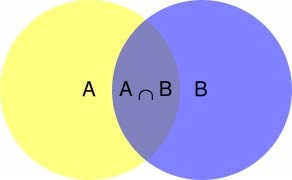
\includegraphics{./img/ch1/conditional_probability.jpg}

图1.1 条件概率文氏图示意

根据文氏图,可以很清楚地看到在事件B发生的情况下,事件A发生的概率就是\(P(A\bigcap B)\)除以\(P(B)\).\\
​举例:一对夫妻有两个小孩,已知其中一个是女孩,则另一个是女孩子的概率是多少?(面试、笔试都碰到过)\\
​\textbf{穷举法}:已知其中一个是女孩,那么样本空间为男女,女女,女男,则另外一个仍然是女生的概率就是1/3.\\
​\textbf{条件概率法}:\(P(女|女)=P(女女)/P(女)\),夫妻有两个小孩,那么它的样本空间为女女,男女,女男,男男,则\(P(女女)\)为1/4,\(P(女)= 1-P(男男)=3/4\),所以最后\(1/3\).\\
这里大家可能会误解,男女和女男是同一种情况,但实际上类似姐弟和兄妹是不同情况.

\subsection{联合概率与边缘概率联系区别}\label{ux8054ux5408ux6982ux7387ux4e0eux8fb9ux7f18ux6982ux7387ux8054ux7cfbux533aux522b}

\textbf{区别:}\\
​联合概率:联合概率指类似于\(P(X=a,Y=b)\)这样,包含多个条件,且所有条件同时成立的概率.联合概率是指在多元的概率分布中多个随机变量分别满足各自条件的概率.\\
​边缘概率:边缘概率是某个事件发生的概率,而与其它事件无关.边缘概率指类似于\(P(X=a)\),\(P(Y=b)\)这样,仅与单个随机变量有关的概率.

\textbf{联系:}\\
​联合分布可求边缘分布,但若只知道边缘分布,无法求得联合分布.

\subsection{条件概率的链式法则}\label{ux6761ux4ef6ux6982ux7387ux7684ux94feux5f0fux6cd5ux5219}

由条件概率的定义,可直接得出下面的乘法公式:\\
​乘法公式 设\(A, B\)是两个事件,并且\(P(A) > 0\), 则有 \[
P(AB) = P(B|A)P(A)
\] 推广 \[
P(ABC)=P(C|AB)P(B|A)P(A)
\] 一般地,用归纳法可证:若\(P(A_1A_2...A_n)>0\),则有 \[
P(A_1A_2...A_n)=P(A_n|A_1A_2...A_{n-1})P(A_{n-1}|A_1A_2...A_{n-2})...P(A_2|A_1)P(A_1)
=P(A_1)\prod_{i=2}^{n}P(A_i|A_1A_2...A_{i-1})
\]
任何多维随机变量联合概率分布,都可以分解成只有一个变量的条件概率相乘形式.

\subsection{独立性和条件独立性}\label{ux72ecux7acbux6027ux548cux6761ux4ef6ux72ecux7acbux6027}

\textbf{独立性}
​两个随机变量\(x\)和\(y\),概率分布表示成两个因子乘积形式,一个因子只包含\(x\),另一个因子只包含\(y\),两个随机变量相互独立(independent).\\
​条件有时为不独立的事件之间带来独立,有时也会把本来独立的事件,因为此条件的存在,而失去独立性.\\
​举例:\(P(XY)=P(X)P(Y)\), 事件\(X\)和事件\(Y\)独立.此时给定\(Z\), \[
P(X,Y|Z) \not = P(X|Z)P(Y|Z)
\]
事件独立时,联合概率等于概率的乘积.这是一个非常好的数学性质,然而不幸的是,无条件的独立是十分稀少的,因为大部分情况下,事件之间都是互相影响的.

\textbf{条件独立性}\\
​给定\(Z\)的情况下,\(X\)和\(Y\)条件独立,当且仅当 \[
X\bot Y|Z \iff P(X,Y|Z) = P(X|Z)P(Y|Z)
\] \(X\)和\(Y\)的关系依赖于\(Z\),而不是直接产生.

\begin{quote}
\textbf{举例}定义如下事件:\\
\(X\):明天下雨;\\
\(Y\):今天的地面是湿的;\\
\(Z\):今天是否下雨;\\
\(Z\)事件的成立,对\(X\)和\(Y\)均有影响,然而,在\(Z\)事件成立的前提下,今天的地面情况对明天是否下雨没有影响.
\end{quote}

\section{常见概率分布}\label{ux5e38ux89c1ux6982ux7387ux5206ux5e03}

\subsection{ Bernoulli分布}\label{bernoulliux5206ux5e03}

\textbf{Bernoulli分布}(伯努利分布,0-1分布)是单个二值随机变量分布,
单参数\(\phi\)∈{[}0,1{]}控制,\(\phi\)给出随机变量等于1的概率.
主要性质有: 
\begin{align*}
P(x=1) &= \phi \\
P(x=0) &= 1-\phi  \\
概率质量函数:P(x=x) &= \phi^x(1-\phi)^{1-x} \\
\end{align*}
 其期望和方差为: 
\begin{align*}
E_x[x] &= \phi \\
Var_x(x) &= \phi{(1-\phi)}
\end{align*}
 \textbf{适用范围}:
\textbf{伯努利分布}适合对\textbf{离散型}随机变量建模.

\textbf{Multinoulli分布}也叫\textbf{范畴分布},
是单个\emph{k}值随机分布,经常用来表示\textbf{对象分类的分布}.
其中\(k\)是有限值.Multinoulli分布由向量\(\vec{p}\in[0,1]^{k-1}\)参数化,每个分量\(p_i\)表示第\(i\)个状态的概率,
且\(p_k=1-1^Tp\).这里\(1^T\)表示元素全为1的列向量的转置,其实就是对于向量p中除了k的概率之和.可以重写为\(p_k=1-\sum_{0}^{k-1}p_i\)
.

补充二项分布、多项分布:

二项分布,通俗点硬币抛多次.二项分布(Binomial
distribution)是\textbf{n重伯努利试验}成功次数的离散概率分布.

多项式分布(Multinomial
Distribution)是二项式分布的推广.二项式做n次伯努利实验,规定了每次试验的结果只有两个,如果现在还是做n次试验,只不过每次试验的结果可以有多m个,且m个结果发生的概率互斥且和为1,则发生其中一个结果X次的概率就是多项式分布.

\subsection{ 高斯分布}\label{ux9ad8ux65afux5206ux5e03}

高斯也叫正态分布(Normal Distribution), 概率度函数如下:\\
\[
N(x;\mu,\sigma^2) = \sqrt{\frac{1}{2\pi\sigma^2}}exp\left ( -\frac{1}{2\sigma^2}(x-\mu)^2 \right )
\] 其中, \(\mu​\)和\(\sigma​\)分别是均值和方差,
中心峰值x坐标由\(\mu​\)给出, 峰的宽度受\(\sigma​\)控制,
最大点在\(x=\mu​\)处取得, 拐点为\(x=\mu\pm\sigma​\)

正态分布中,±1\(\sigma\)、±2\(\sigma\)、±3\(\sigma\)下的概率分别是68.3\%、95.5\%、99.73\%,这3个数最好记住.

此外, 令\(\mu=0,\sigma=1​\)高斯分布即简化为标准正态分布: \[
N(x;\mu,\sigma^2) = \sqrt{\frac{1}{2\pi}}exp\left ( -\frac{1}{2}x^2 \right )
\] 对概率密度函数高效求值: \[
N(x;\mu,\beta^{-1})=\sqrt{\frac{\beta}{2\pi}}exp\left(-\frac{1}{2}\beta(x-\mu)^2\right)
\]

其中,\(\beta=\frac{1}{\sigma^2}\)通过参数\(\beta∈(0,\infty)​\)来控制分布精度.

\subsection{何时采用正态分布}\label{ux4f55ux65f6ux91c7ux7528ux6b63ux6001ux5206ux5e03}

问: 何时采用正态分布? 答: 缺乏实数上分布的先验知识, 不知选择何种形式时,
默认选择正态分布总是不会错的, 理由如下:

\begin{enumerate}
\def\labelenumi{\arabic{enumi}.}
 
\item
  中心极限定理告诉我们, 很多独立随机变量均近似服从正态分布,
  现实中很多复杂系统都可以被建模成正态分布的噪声,
  即使该系统可以被结构化分解.
\item
  正态分布是具有相同方差的所有概率分布中, 不确定性最大的分布, 换句话说,
  正态分布是对模型加入先验知识最少的分布.
\end{enumerate}

正态分布的推广: 正态分布可以推广到\(R^n\)空间,
此时称为\textbf{多位正态分布}, 其参数是一个正定对称矩阵\(\Sigma​\): \[
N(x;\vec\mu,\Sigma)=\sqrt{\frac{1}{(2\pi)^ndet(\Sigma)}}exp\left(-\frac{1}{2}(\vec{x}-\vec{\mu})^T\Sigma^{-1}(\vec{x}-\vec{\mu})\right)
\] 对多为正态分布概率密度高效求值: \[
N(x;\vec{\mu},\vec\beta^{-1}) = \sqrt{det(\vec\beta)}{(2\pi)^n}exp\left(-\frac{1}{2}(\vec{x}-\vec\mu)^T\beta(\vec{x}-\vec\mu)\right)
\] 此处,\(\vec\beta\)是一个精度矩阵.

\subsection{ 指数分布}\label{ux6307ux6570ux5206ux5e03}

深度学习中, 指数分布用来描述在\(x=0​\)点处取得边界点的分布,
指数分布定义如下: \[
p(x;\lambda)=\lambda I_{x\geq 0}exp(-\lambda{x})
\] 指数分布用指示函数\(I_{x\geq 0}​\)来使\(x​\)取负值时的概率为零.

\subsection{ Laplace分布(拉普拉斯分布)}\label{laplace-ux5206ux5e03ux62c9ux666eux62c9ux65afux5206ux5e03}

一个联系紧密的概率分布是 Laplace 分布(Laplace
distribution),它允许我们在任意一点 \(\mu\)处设置概率质量的峰值 \[
Laplace(x;\mu;\gamma)=\frac{1}{2\gamma}exp\left(-\frac{|x-\mu|}{\gamma}\right)
\]

\subsection{Dirac分布和经验分布}\label{diracux5206ux5e03ux548cux7ecfux9a8cux5206ux5e03}

Dirac分布可保证概率分布中所有质量都集中在一个点上.
Diract分布的狄拉克\(\delta​\)函数(也称为\textbf{单位脉冲函数})定义如下:
\[
p(x)=\delta(x-\mu), x\neq \mu
\]

\[
\int_{a}^{b}\delta(x-\mu)dx = 1, a < \mu < b
\]

Dirac 分布经常作为 经验分布(empirical distribution)的一个组成部分出现
\[
\hat{p}(\vec{x})=\frac{1}{m}\sum_{i=1}^{m}\delta(\vec{x}-{\vec{x}}^{(i)})
\] , 其中, m个点\(x^{1},...,x^{m}\)是给定的数据集,
\textbf{经验分布}将概率密度\(\frac{1}{m}​\)赋给了这些点.

当我们在训练集上训练模型时,
可以认为从这个训练集上得到的经验分布指明了\textbf{采样来源}.

\textbf{适用范围}: 狄拉克δ函数适合对\textbf{连续型}随机变量的经验分布.

\begin{quote}
\end{quote}

\section{期望、方差、协方差、相关系数}\label{ux671fux671bux65b9ux5deeux534fux65b9ux5deeux76f8ux5173ux7cfbux6570}

\subsection{ 期望}\label{ux671fux671b}

在概率论和统计学中,数学期望(或均值,亦简称期望)是试验中每次可能结果的概率乘以其结果的总和.它反映随机变量平均取值的大小.

\begin{itemize}
 
\item
  线性运算: \(E(ax+by+c) = aE(x)+bE(y)+c\)\\
\item
  推广形式:
  \(E(\sum_{k=1}^{n}{a_ix_i+c}) = \sum_{k=1}^{n}{a_iE(x_i)+c}\)
\item
  函数期望:设\(f(x)\)为\(x\)的函数,则\(f(x)\)的期望为

  \begin{itemize}
   
  \item
    离散函数: \(E(f(x))=\sum_{k=1}^{n}{f(x_k)P(x_k)}\)
  \item
    连续函数: \(E(f(x))=\int_{-\infty}^{+\infty}{f(x)p(x)dx}\)
  \end{itemize}
\end{itemize}

\begin{quote}
注意:

\begin{itemize}
 \item
  函数的期望大于等于期望的函数(Jensen(詹森)不等式,即\(E(f(x))\geqslant f(E(x))\)\\
\item
  一般情况下,乘积的期望不等于期望的乘积.\\
\item
  如果\(X\)和\(Y\)相互独立,则\(E(xy)=E(x)E(y)​\).
\end{itemize}
\end{quote}

\subsection{方差}\label{ux65b9ux5dee}

概率论中方差用来度量随机变量和其数学期望(即均值)之间的偏离程度.方差是一种特殊的期望.定义为:

\[
Var(x) = E((x-E(x))^2)
\]

\begin{quote}
方差性质:

1)\(Var(x) = E(x^2) -E(x)^2\)\\
2)常数的方差为0;\\
3)方差不满足线性性质;\\
4)如果\(X\)和\(Y\)相互独立, \(Var(ax+by)=a^2Var(x)+b^2Var(y)\)
\end{quote}

\subsection{ 协方差}\label{ux534fux65b9ux5dee}

协方差是衡量两个变量线性相关性强度及变量尺度.
两个随机变量的协方差定义为: \[
Cov(x,y)=E((x-E(x))(y-E(y)))
\]

方差是一种特殊的协方差.当\(X=Y\)时,\(Cov(x,y)=Var(x)=Var(y)\).

\begin{quote}
协方差性质:

1)独立变量的协方差为0.\\
2)协方差计算公式:
\end{quote}

\[
Cov(\sum_{i=1}^{m}{a_ix_i}, \sum_{j=1}^{m}{b_jy_j}) = \sum_{i=1}^{m} \sum_{j=1}^{m}{a_ib_jCov(x_iy_i)}
\]

\begin{quote}
3)特殊情况:
\end{quote}

\[
Cov(a+bx, c+dy) = bdCov(x, y)
\]

\subsection{ 相关系数}\label{ux76f8ux5173ux7cfbux6570}

相关系数是研究变量之间线性相关程度的量.两个随机变量的相关系数定义为:
\[
Corr(x,y) = \frac{Cov(x,y)}{\sqrt{Var(x)Var(y)}}
\]

\begin{quote}
相关系数的性质:\\
1)有界性.相关系数的取值范围是 {[}-1,1{]},可以看成无量纲的协方差.\\
2)值越接近1,说明两个变量正相关性(线性)越强.越接近-1,说明负相关性越强,当为0时,表示两个变量没有相关性.
\end{quote}

% \section{参考文献}\label{ux53c2ux8003ux6587ux732e}

% {[}1{]}Ian,Goodfellow,Yoshua,Bengio,Aaron\ldots{}深度学习{[}M{]},人民邮电出版,2017

% {[}2{]}周志华.机器学习{[}M{]}.清华大学出版社,2016.

% {[}3{]}同济大学数学系.高等数学(第七版){[}M{]},高等教育出版社,2014.

% {[}4{]}盛骤,试式千,潘承毅等编.
% 概率论与数理统计(第4版){[}M{]},高等教育出版社,2008

\chapter{机器学习基础}
\label{ux7b2cux4e8cux7ae0-ux673aux5668ux5b66ux4e60ux57faux7840}
​ 机器学习起源于上世纪50年代,1959年在IBM工作的Arthur
Samuel设计了一个下棋程序,这个程序具有学习的能力,它可以在不断的对弈中提高自己。由此提出了``机器学习''这个概念,它是一个结合了多个学科如概率论,优化理论,统计等,最终在计算机上实现自我获取新知识,学习改善自己的这样一个研究领域。机器学习是人工智能的一个子集,目前已经发展出许多有用的方法,比如支持向量机,回归,决策树,随机森林,强化方法,集成学习,深度学习等等,一定程度上可以帮助人们完成一些数据预测,自动化,自动决策,最优化等初步替代脑力的任务。本章我们主要介绍下机器学习的基本概念、监督学习、分类算法、逻辑回归、代价函数、损失函数、LDA、PCA、决策树、支持向量机、EM算法、聚类和降维以及模型评估有哪些方法、指标等等。

\section{ 基本概念}\label{ux57faux672cux6982ux5ff5}

\subsection{大话理解机器学习本质}\label{ux5927ux8bddux7406ux89e3ux673aux5668ux5b66ux4e60ux672cux8d28}

​ 机器学习(Machine Learning,
ML),顾名思义,让机器去学习。这里,机器指的是计算机,是算法运行的物理载体,你也可以把各种算法本身当做一个有输入和输出的机器。那么到底让计算机去学习什么呢?对于一个任务及其表现的度量方法,设计一种算法,让算法能够提取中数据所蕴含的规律,这就叫机器学习。如果输入机器的数据是带有标签的,就称作有监督学习。如果数据是无标签的,就是无监督学习。

\subsection{什么是神经网络}\label{ux4ec0ux4e48ux662fux795eux7ecfux7f51ux7edc}

​
神经网络就是按照一定规则将多个神经元连接起来的网络。不同的神经网络,具有不同的连接规则。例如全连接(Full
Connected, FC)神经网络,它的规则包括:

(1)有三种层:输入层,输出层,隐藏层。

(2)同一层的神经元之间没有连接。

(3)fully connected的含义:第 N 层的每个神经元和第 N-1
层的所有神经元相连,第 N-1 层神经元的输出就是第 N 层神经元的输入。

(4)每个连接都有一个权值。

\textbf{神经网络架构} ​
图2-1就是一个神经网络系统,它由很多层组成。输入层负责接收信息,比如一只猫的图片。输出层是计算机对这个输入信息的判断结果,它是不是猫。隐藏层就是对输入信息的传递和加工处理。
% 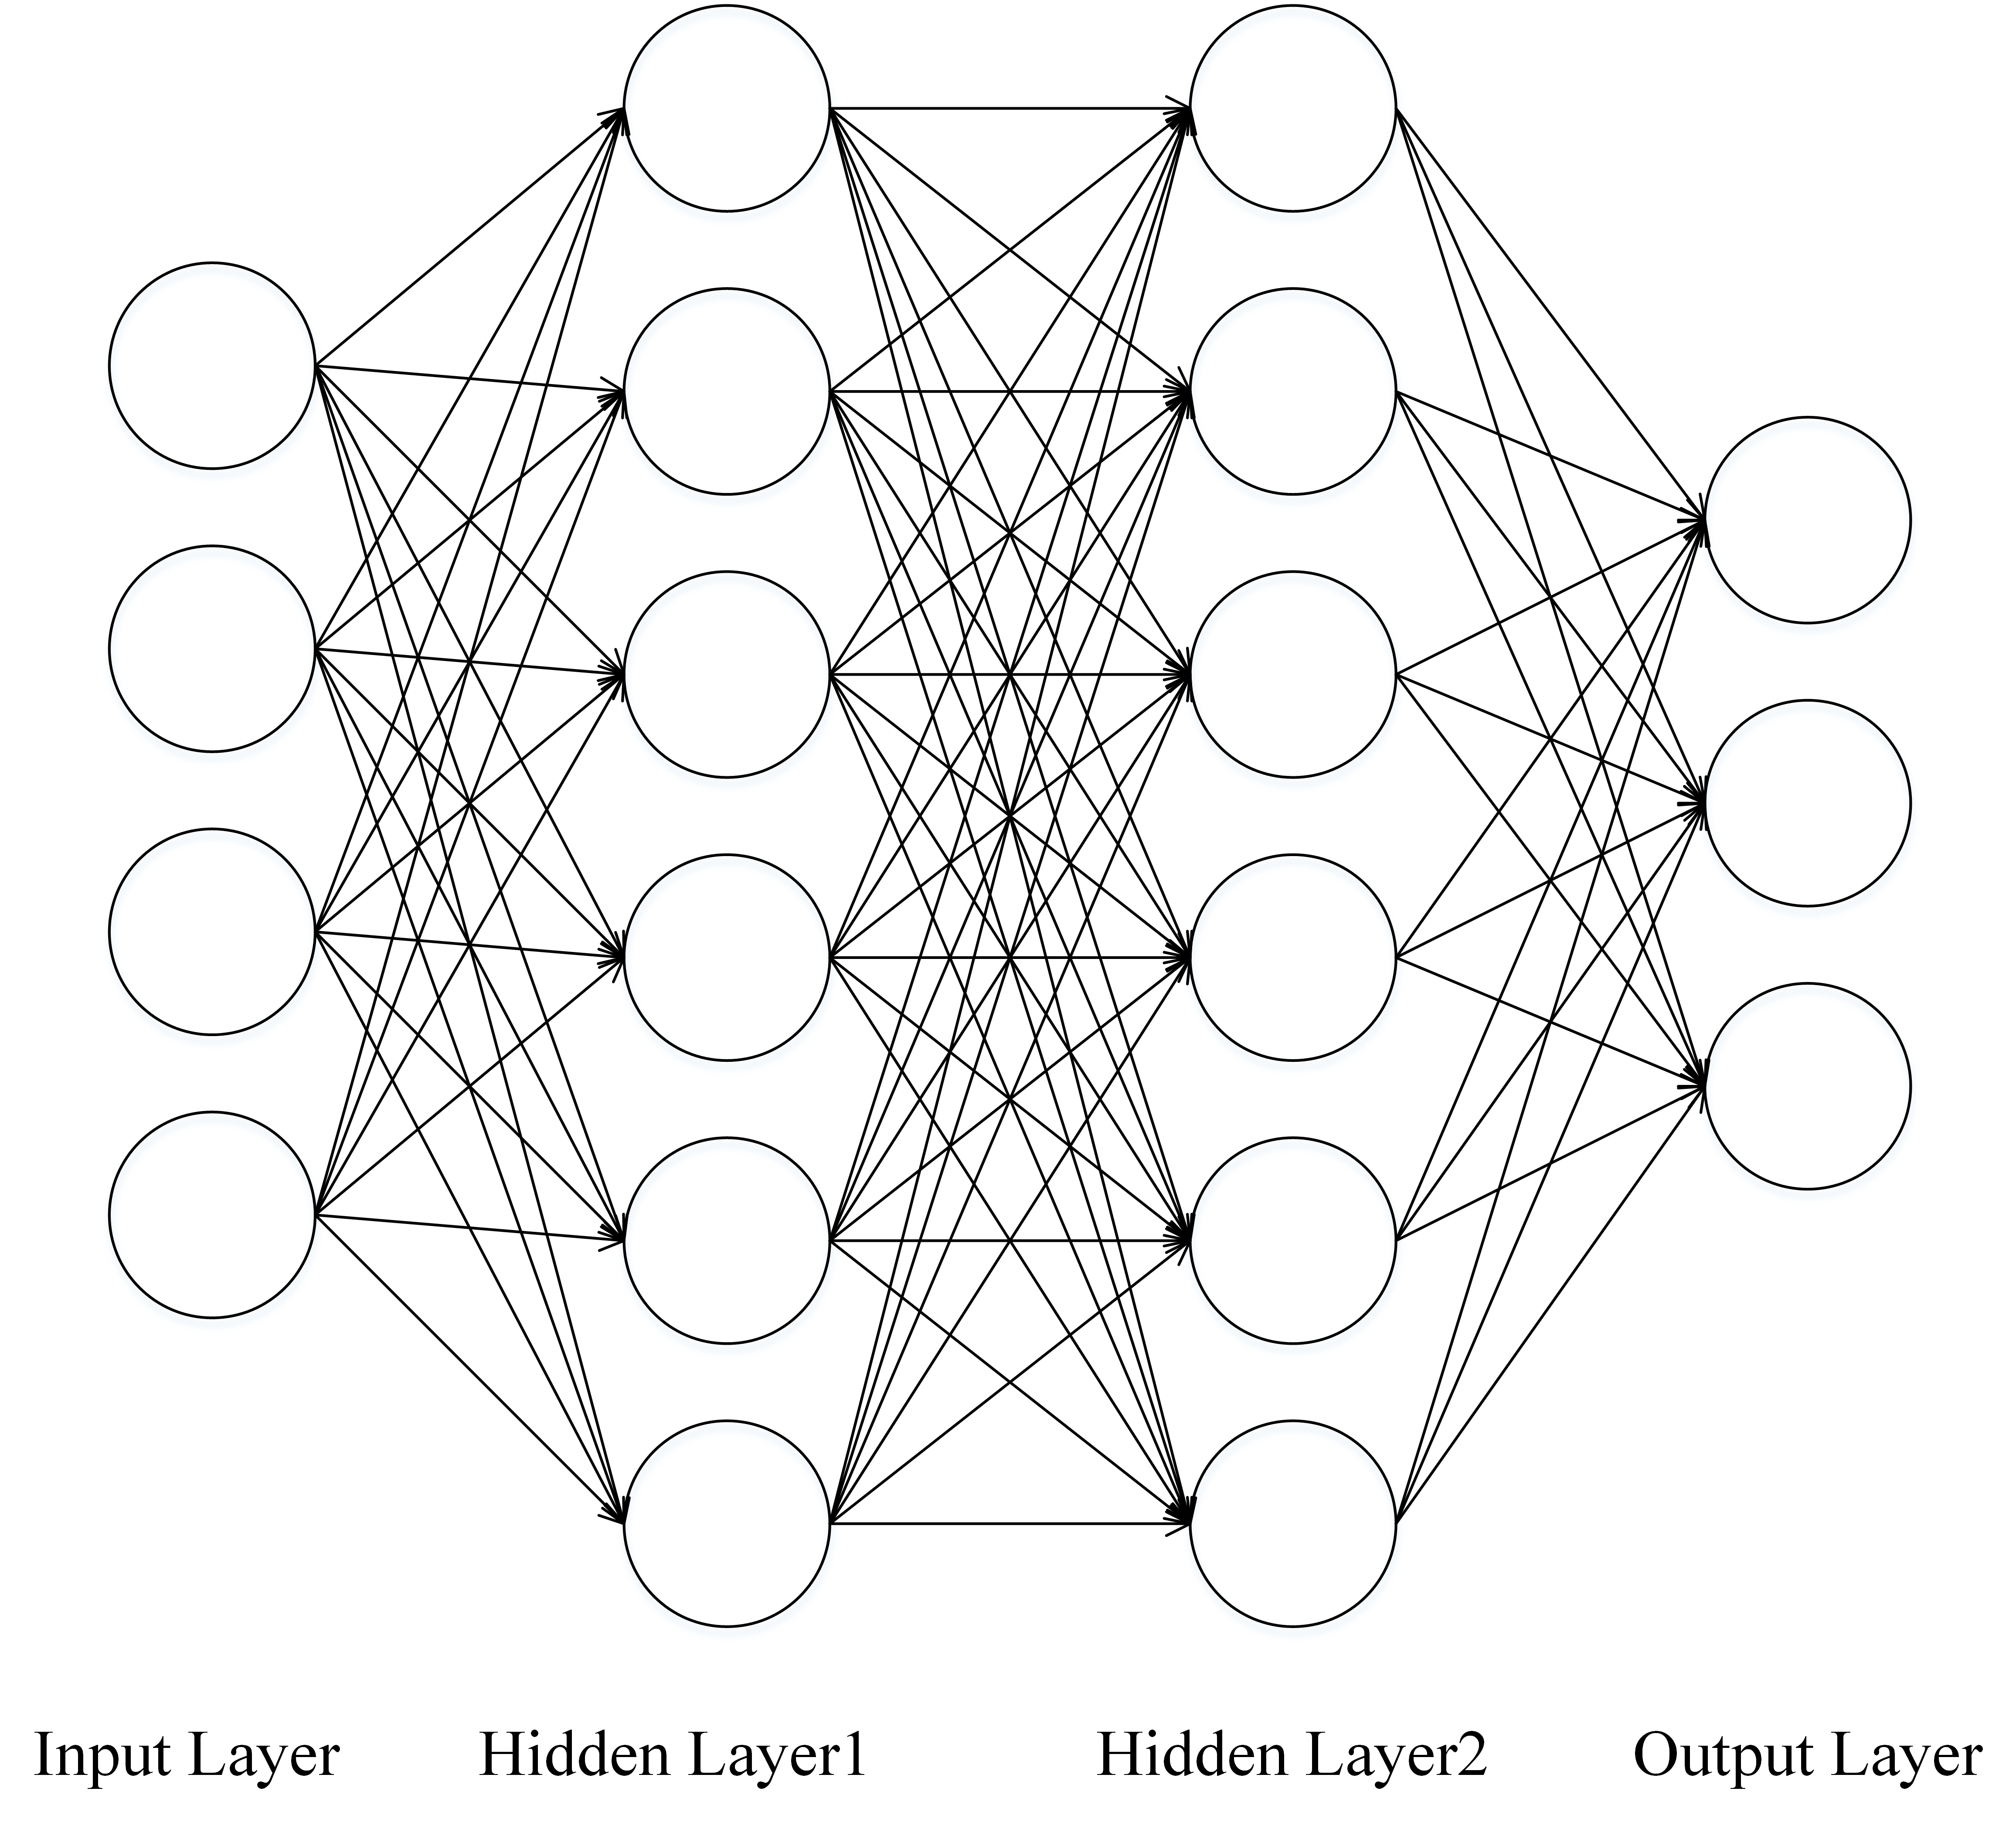
\includegraphics{./img/ch2/2.5.1.png}

​ 图2-1 神经网络系统

\subsection{各种常见算法图示}\label{ux5404ux79cdux5e38ux89c1ux7b97ux6cd5ux56feux793a}

​
日常使用机器学习的任务中,我们经常会遇见各种算法,图2-2是各种常见算法的图示。

% \begin{longtable}[]{ccc}
% %\toprule
% 回归算法 & 聚类算法 & 正则化方法\tabularnewline
% %\midrule
% %\endhead
% 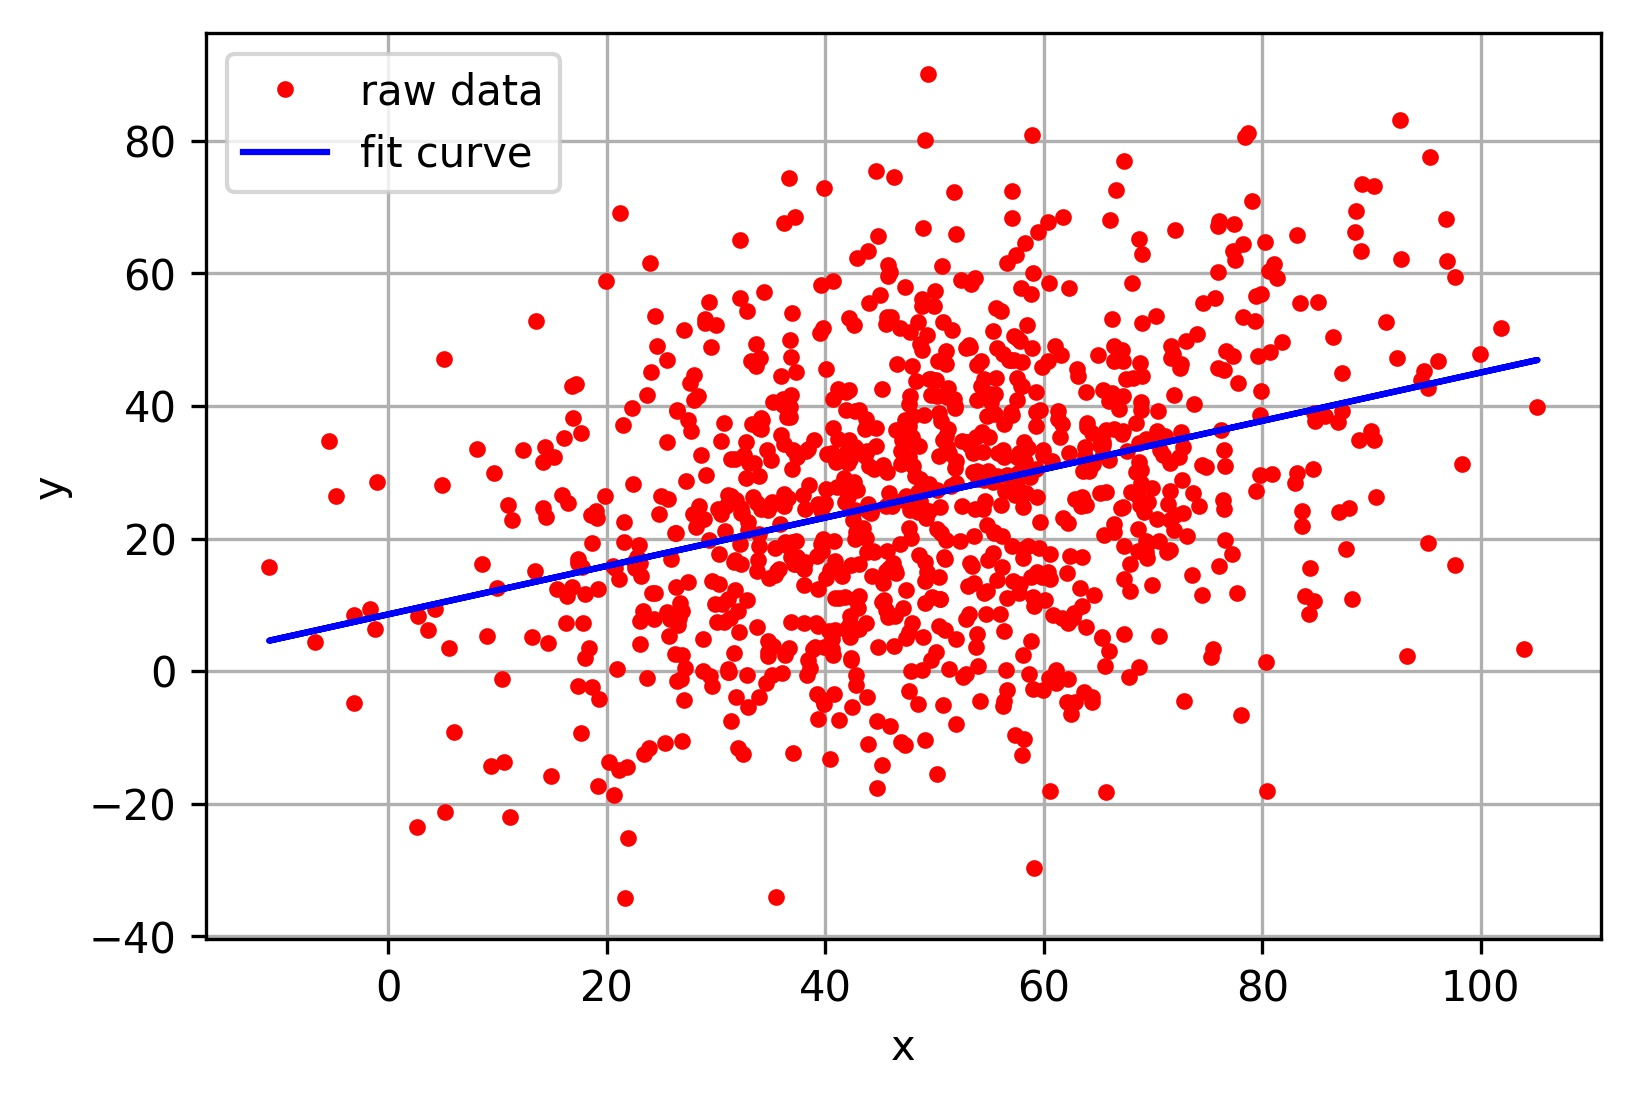
\includegraphics{./img/ch2/2.1/1.jpg} &
% 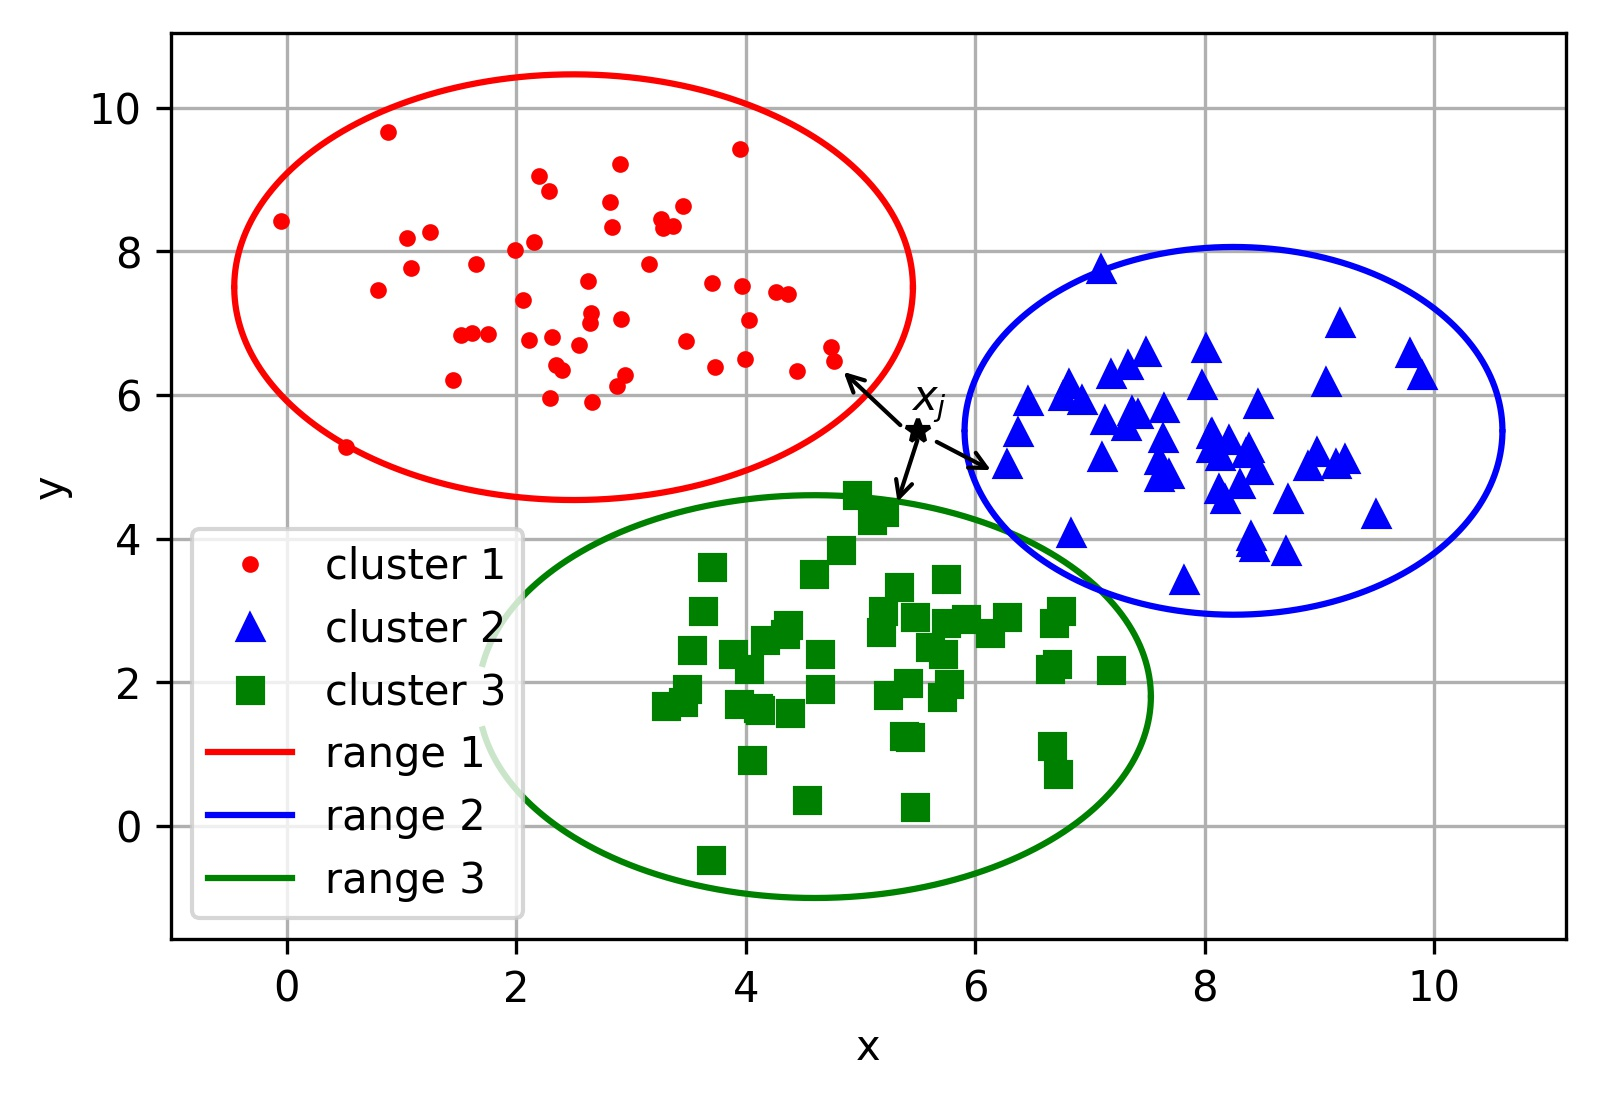
\includegraphics{./img/ch2/2.1/2.jpg} &
% 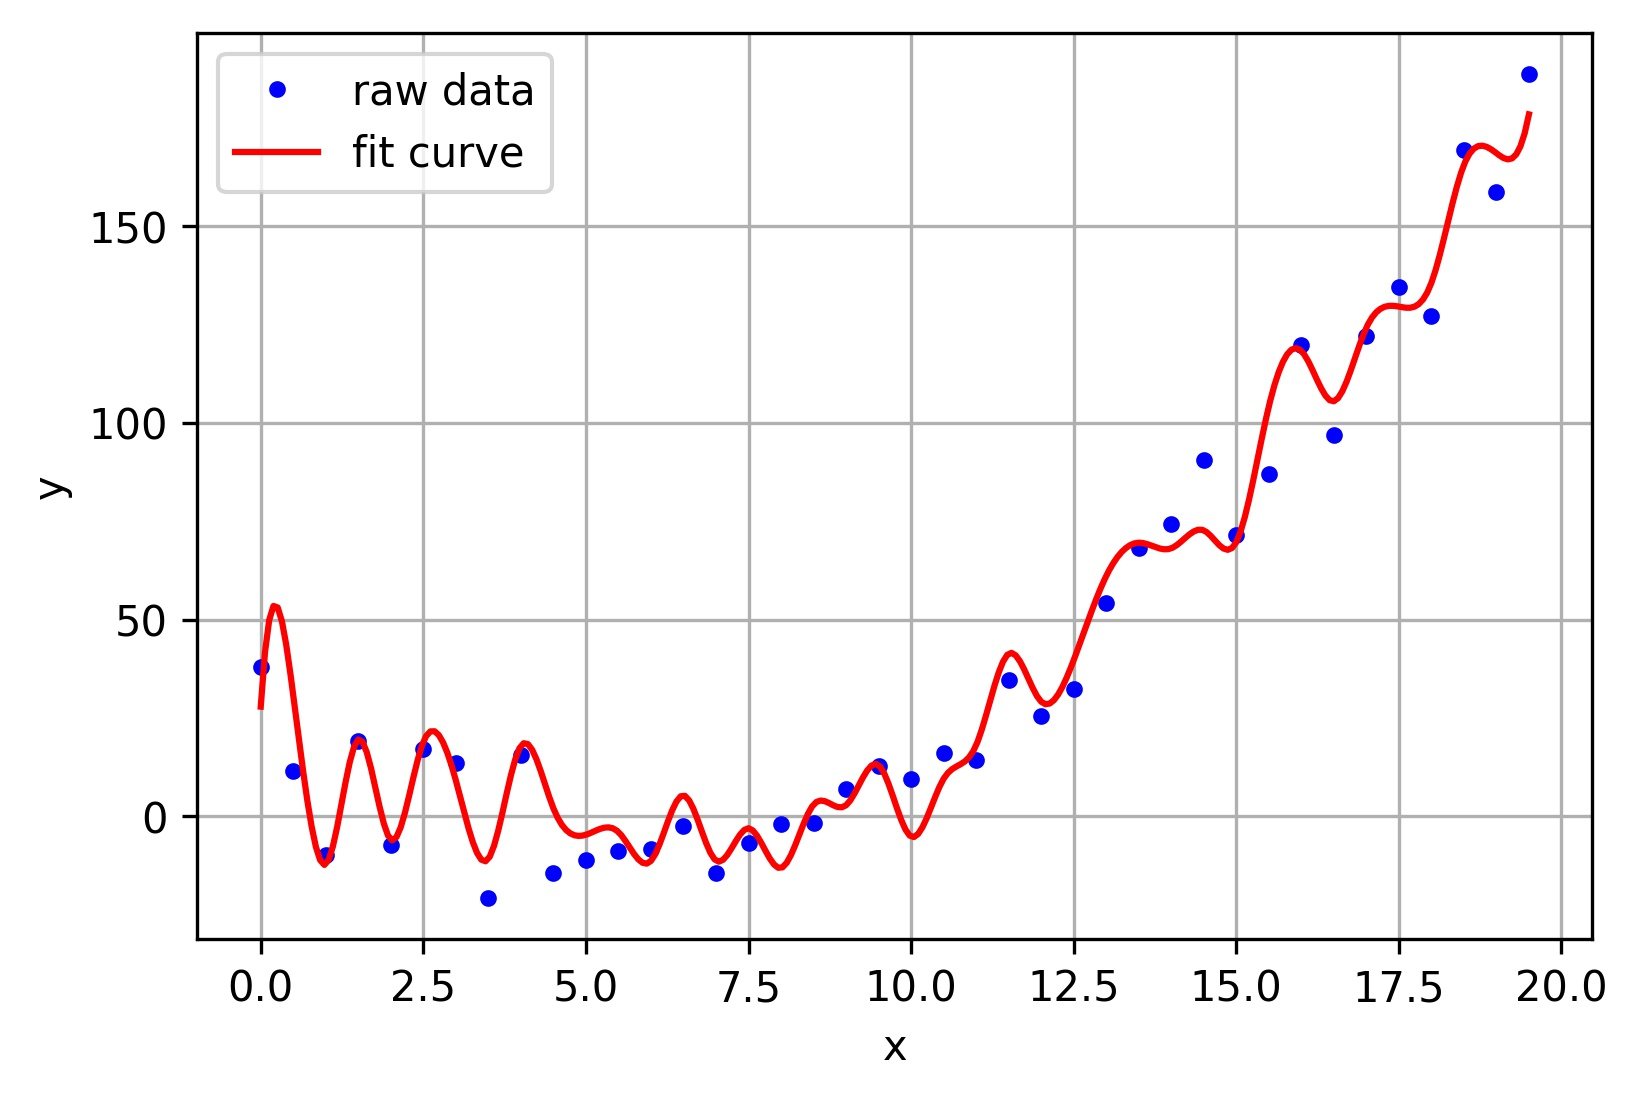
\includegraphics{./img/ch2/2.1/3.jpg}\tabularnewline
% % \bottomrule
% \end{longtable}

% \begin{longtable}[]{ccc}
% %\toprule
% 决策树学习 & 贝叶斯方法 & 基于核的算法\tabularnewline
% %\midrule
% %\endhead
% 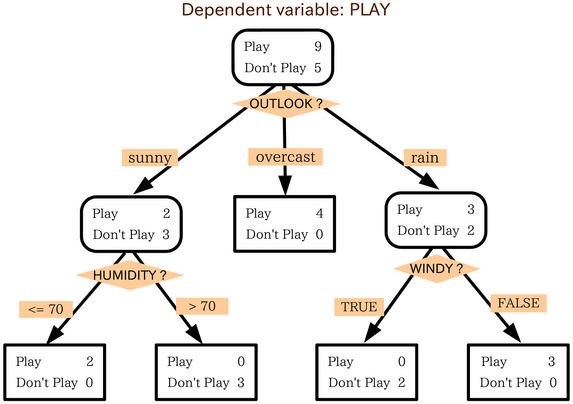
\includegraphics{./img/ch2/2.2.4.png} &
% 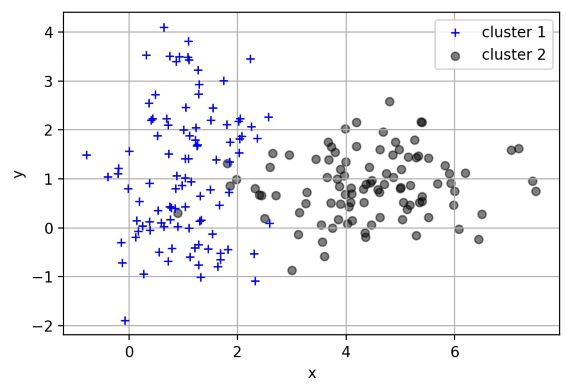
\includegraphics{./img/ch2/2.1/5.jpg} &
% 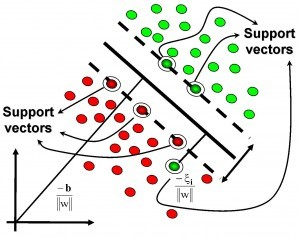
\includegraphics{./img/ch2/2.1/6.jpg}\tabularnewline
% % \bottomrule
% \end{longtable}

% \begin{longtable}[]{ ccc }
% %\toprule
% 聚类算法 & 关联规则学习 & 人工神经网络\tabularnewline
% %\midrule
% %\endhead
% 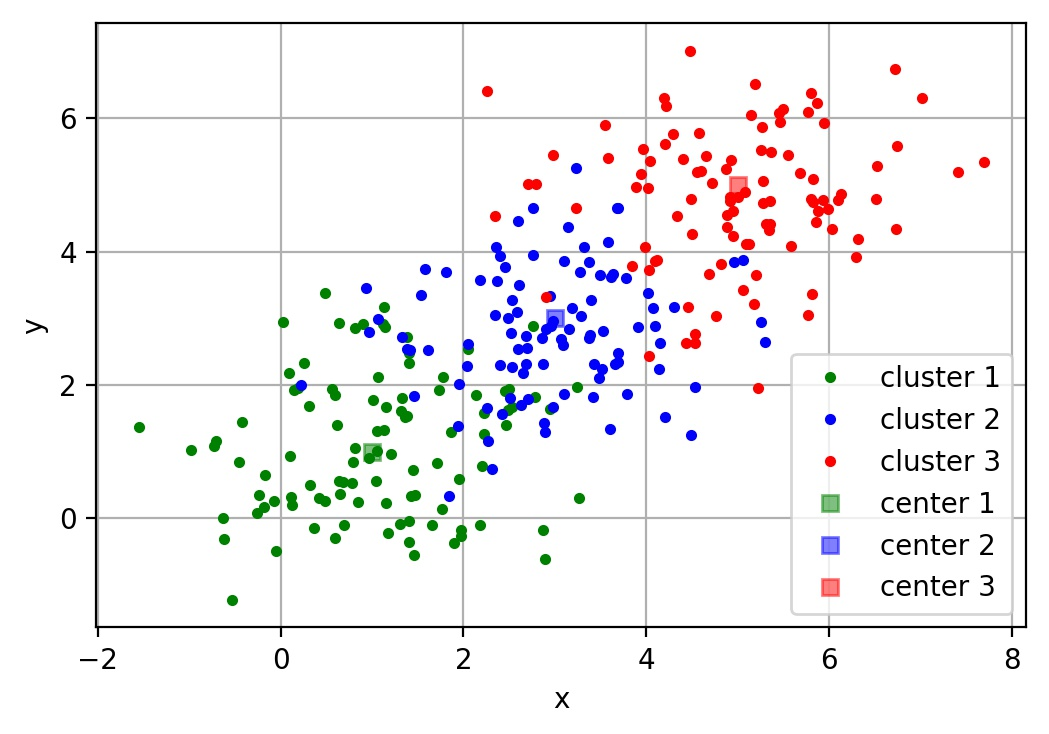
\includegraphics{./img/ch2/2.1/7.jpg} &
% 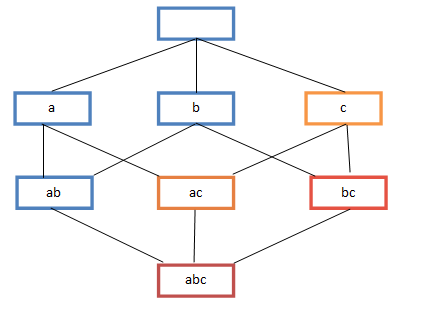
\includegraphics{./img/ch2/2.2.8.png} &
% 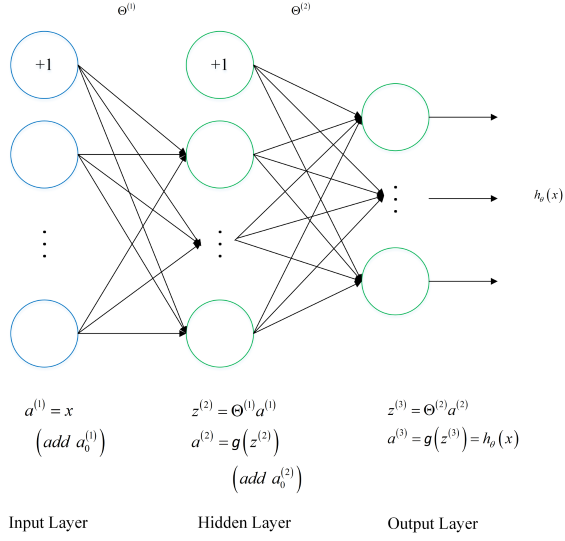
\includegraphics{./img/ch2/2.2.09.png}\tabularnewline
% % \bottomrule
% \end{longtable}

% \begin{longtable}[]{ccc}
% %\toprule
% 深度学习 & 降低维度算法 & 集成算法\tabularnewline
% %\midrule
% %\endhead
% 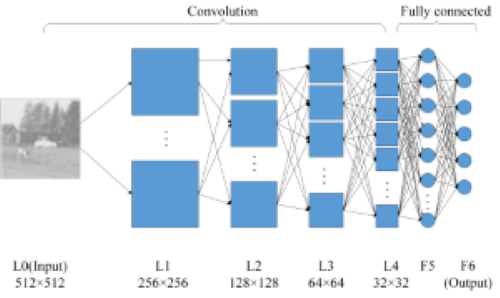
\includegraphics{./img/ch2/2.2.10.png} &
% 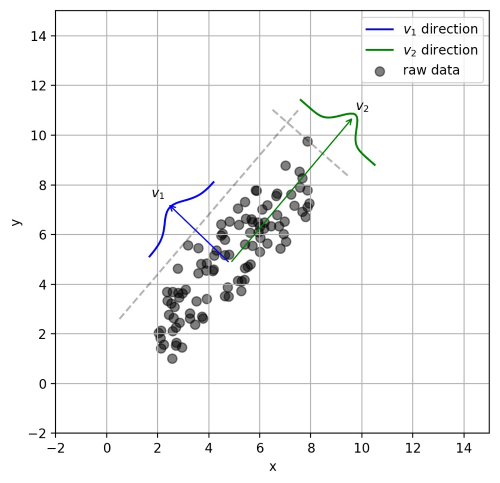
\includegraphics{./img/ch2/2.2.11.png} &
% 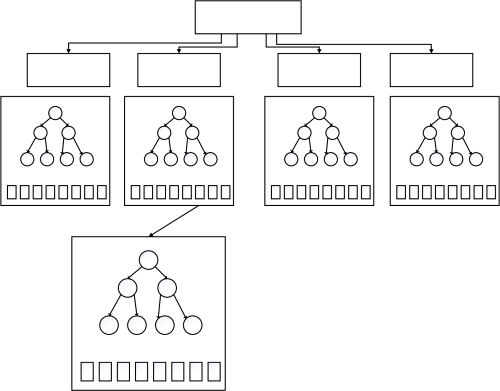
\includegraphics{./img/ch2/2.2.12.png}\tabularnewline
% % \bottomrule
% \end{longtable}

​ 图2-2 各种常见算法图示

\subsection{计算图的导数计算}\label{ux8ba1ux7b97ux56feux7684ux5bfcux6570ux8ba1ux7b97}

​ 计算图导数计算是反向传播,利用链式法则和隐式函数求导。

​ 假设 $z = f(u,v)$ 在点 $(u,v)$ 处偏导连续,$(u,v)$是关于 $t$
的函数,在 $t$ 点可导,求 $z$ 在 $t$ 点的导数。

根据链式法则有 \[
\frac{dz}{dt}=\frac{\partial z}{\partial u}.\frac{du}{dt}+\frac{\partial z}{\partial v}
                .\frac{dv}{dt}
\] ​
链式法则用文字描述:``由两个函数凑起来的复合函数,其导数等于里边函数代入外边函数的值之导数,乘以里边函数的导数。\\
​ 为了便于理解,下面举例说明: \[
f(x)=x^2,g(x)=2x+1
\] ​ 则: \[
{f[g(x)]}'=2[g(x)] \times g'(x)=2[2x+1] \times 2=8x+4
\]

\subsection{理解局部最优与全局最优}\label{ux7406ux89e3ux5c40ux90e8ux6700ux4f18ux4e0eux5168ux5c40ux6700ux4f18}

​ 笑谈局部最优和全局最优

\begin{quote}
​
柏拉图有一天问老师苏格拉底什么是爱情?苏格拉底叫他到麦田走一次,摘一颗最大的麦穗回来,不许回头,只可摘一次。柏拉图空着手出来了,他的理由是,看见不错的,却不知道是不是最好的,一次次侥幸,走到尽头时,才发现还不如前面的,于是放弃。苏格拉底告诉他:``这就是爱情。''这故事让我们明白了一个道理,因为生命的一些不确定性,所以全局最优解是很难寻找到的,或者说根本就不存在,我们应该设置一些限定条件,然后在这个范围内寻找最优解,也就是局部最优解------有所斩获总比空手而归强,哪怕这种斩获只是一次有趣的经历。
​
柏拉图有一天又问什么是婚姻?苏格拉底叫他到树林走一次,选一棵最好的树做圣诞树,也是不许回头,只许选一次。这次他一身疲惫地拖了一棵看起来直挺、翠绿,却有点稀疏的杉树回来,他的理由是,有了上回的教训,好不容易看见一棵看似不错的,又发现时间、体力已经快不够用了,也不管是不是最好的,就拿回来了。苏格拉底告诉他:``这就是婚姻。''
\end{quote}

​ 优化问题一般分为局部最优和全局最优。其中,

(1)局部最优,就是在函数值空间的一个有限区域内寻找最小值;而全局最优,是在函数值空间整个区域寻找最小值问题。

(2)函数局部最小点是它的函数值小于或等于附近点的点,但是有可能大于较远距离的点。

(3)全局最小点是那种它的函数值小于或等于所有的可行点。

\subsection{大数据与深度学习之间的关系}\label{ux5927ux6570ux636eux4e0eux6df1ux5ea6ux5b66ux4e60ux4e4bux95f4ux7684ux5173ux7cfb}

首先来看大数据、机器学习及数据挖掘三者简单的定义:

\textbf{大数据}通常被定义为``超出常用软件工具捕获,管理和处理能力''的数据集。
\textbf{机器学习}关心的问题是如何构建计算机程序使用经验自动改进。
\textbf{数据挖掘}是从数据中提取模式的特定算法的应用,在数据挖掘中,重点在于算法的应用,而不是算法本身。

\textbf{机器学习和数据挖掘}之间的关系如下:
数据挖掘是一个过程,在此过程中机器学习算法被用作提取数据集中的潜在有价值模式的工具。
大数据与深度学习关系总结如下:

(1)深度学习是一种模拟大脑的行为。可以从所学习对象的机制以及行为等等很多相关联的方面进行学习,模仿类型行为以及思维。

(2)深度学习对于大数据的发展有帮助。深度学习对于大数据技术开发的每一个阶段均有帮助,不管是数据的分析还是挖掘还是建模,只有深度学习,这些工作才会有可能一一得到实现。

(3)深度学习转变了解决问题的思维。很多时候发现问题到解决问题,走一步看一步不是一个主要的解决问题的方式了,在深度学习的基础上,要求我们从开始到最后都要基于一个目标,为了需要优化的那个最终目标去进行处理数据以及将数据放入到数据应用平台上去,这就是端到端(End
to End)。

(4)大数据的深度学习需要一个框架。在大数据方面的深度学习都是从基础的角度出发的,深度学习需要一个框架或者一个系统。总而言之,将你的大数据通过深度分析变为现实,这就是深度学习和大数据的最直接关系。

\section{机器学习学习方式}\label{ux673aux5668ux5b66ux4e60ux5b66ux4e60ux65b9ux5f0f}

​
根据数据类型的不同,对一个问题的建模有不同的方式。依据不同的学习方式和输入数据,机器学习主要分为以下四种学习方式。

\subsection{ 监督学习}\label{ux76d1ux7763ux5b66ux4e60}

​
特点:监督学习是使用已知正确答案的示例来训练网络。已知数据和其一一对应的标签,训练一个预测模型,将输入数据映射到标签的过程。

​ 常见应用场景:监督式学习的常见应用场景如分类问题和回归问题。

​ 算法举例:常见的有监督机器学习算法包括支持向量机(Support Vector
Machine, SVM),朴素贝叶斯(Naive Bayes),逻辑回归(Logistic
Regression),K近邻(K-Nearest Neighborhood, KNN),决策树(Decision
Tree),随机森林(Random Forest),AdaBoost以及线性判别分析(Linear
Discriminant Analysis, LDA)等。深度学习(Deep
Learning)也是大多数以监督学习的方式呈现。

\subsection{非监督式学习}\label{ux975eux76d1ux7763ux5f0fux5b66ux4e60}

​
定义:在非监督式学习中,数据并不被特别标识,适用于你具有数据集但无标签的情况。学习模型是为了推断出数据的一些内在结构。

​ 常见应用场景:常见的应用场景包括关联规则的学习以及聚类等。

​ 算法举例:常见算法包括Apriori算法以及k-Means算法。

\subsection{半监督式学习}\label{ux534aux76d1ux7763ux5f0fux5b66ux4e60}

​
特点:在此学习方式下,输入数据部分被标记,部分没有被标记,这种学习模型可以用来进行预测。

​
常见应用场景:应用场景包括分类和回归,算法包括一些对常用监督式学习算法的延伸,通过对已标记数据建模,在此基础上,对未标记数据进行预测。

​ 算法举例:常见算法如图论推理算法(Graph
Inference)或者拉普拉斯支持向量机(Laplacian SVM)等。

\subsection{弱监督学习}\label{ux5f31ux76d1ux7763ux5b66ux4e60}

​
特点:弱监督学习可以看做是有多个标记的数据集合,次集合可以是空集,单个元素,或包含多种情况(没有标记,有一个标记,和有多个标记)的多个元素。
数据集的标签是不可靠的,这里的不可靠可以是标记不正确,多种标记,标记不充分,局部标记等。已知数据和其一一对应的弱标签,训练一个智能算法,将输入数据映射到一组更强的标签的过程。标签的强弱指的是标签蕴含的信息量的多少,比如相对于分割的标签来说,分类的标签就是弱标签。

​
算法举例:举例,给出一张包含气球的图片,需要得出气球在图片中的位置及气球和背景的分割线,这就是已知弱标签学习强标签的问题。

​ 在企业数据应用的场景下,
人们最常用的可能就是监督式学习和非监督式学习的模型。
在图像识别等领域,由于存在大量的非标识的数据和少量的可标识数据,
目前半监督式学习是一个很热的话题。

\subsection{监督学习有哪些步骤}\label{ux76d1ux7763ux5b66ux4e60ux6709ux54eaux4e9bux6b65ux9aa4}

​
监督学习是使用已知正确答案的示例来训练网络,每组训练数据有一个明确的标识或结果。想象一下,我们可以训练一个网络,让其从照片库中(其中包含气球的照片)识别出气球的照片。以下就是我们在这个假设场景中所要采取的步骤。

\textbf{步骤1:数据集的创建和分类} ​
首先,浏览你的照片(数据集),确定所有包含气球的照片,并对其进行标注。然后,将所有照片分为训练集和验证集。目标就是在深度网络中找一函数,这个函数输入是任意一张照片,当照片中包含气球时,输出1,否则输出0。

\textbf{步骤2:数据增强(Data Augmentation)} ​
当原始数据搜集和标注完毕,一般搜集的数据并不一定包含目标在各种扰动下的信息。数据的好坏对于机器学习模型的预测能力至关重要,因此一般会进行数据增强。对于图像数据来说,数据增强一般包括,图像旋转,平移,颜色变换,裁剪,仿射变换等。

\textbf{步骤3:特征工程(Feature Engineering)} ​
一般来讲,特征工程包含特征提取和特征选择。常见的手工特征(Hand-Crafted
Feature)有尺度不变特征变换(Scale-Invariant Feature Transform,
SIFT),方向梯度直方图(Histogram of Oriented Gradient,
HOG)等。由于手工特征是启发式的,其算法设计背后的出发点不同,将这些特征组合在一起的时候有可能会产生冲突,如何将组合特征的效能发挥出来,使原始数据在特征空间中的判别性最大化,就需要用到特征选择的方法。在深度学习方法大获成功之后,人们很大一部分不再关注特征工程本身。因为,最常用到的卷积神经网络(Convolutional
Neural Networks,
CNNs)本身就是一种特征提取和选择的引擎。研究者提出的不同的网络结构、正则化、归一化方法实际上就是深度学习背景下的特征工程。

\textbf{步骤4:构建预测模型和损失} ​
将原始数据映射到特征空间之后,也就意味着我们得到了比较合理的输入。下一步就是构建合适的预测模型得到对应输入的输出。而如何保证模型的输出和输入标签的一致性,就需要构建模型预测和标签之间的损失函数,常见的损失函数(Loss
Function)有交叉熵、均方差等。通过优化方法不断迭代,使模型从最初的初始化状态一步步变化为有预测能力的模型的过程,实际上就是学习的过程。

\textbf{步骤5:训练} ​
选择合适的模型和超参数进行初始化,其中超参数比如支持向量机中核函数、误差项惩罚权重等。当模型初始化参数设定好后,将制作好的特征数据输入到模型,通过合适的优化方法不断缩小输出与标签之间的差距,当迭代过程到了截止条件,就可以得到训练好的模型。优化方法最常见的就是梯度下降法及其变种,使用梯度下降法的前提是优化目标函数对于模型是可导的。

\textbf{步骤6:验证和模型选择} ​
训练完训练集图片后,需要进行模型测试。利用验证集来验证模型是否可以准确地挑选出含有气球在内的照片。
​
在此过程中,通常会通过调整和模型相关的各种事物(超参数)来重复步骤2和3,诸如里面有多少个节点,有多少层,使用怎样的激活函数和损失函数,如何在反向传播阶段积极有效地训练权值等等。

\textbf{步骤7:测试及应用} ​
当有了一个准确的模型,就可以将该模型部署到你的应用程序中。你可以将预测功能发布为API(Application
Programming Interface,
应用程序编程接口)调用,并且你可以从软件中调用该API,从而进行推理并给出相应的结果。

\section{ 分类算法}\label{ux5206ux7c7bux7b97ux6cd5}

​
分类算法和回归算法是对真实世界不同建模的方法。分类模型是认为模型的输出是离散的,例如大自然的生物被划分为不同的种类,是离散的。回归模型的输出是连续的,例如人的身高变化过程是一个连续过程,而不是离散的。

​
因此,在实际建模过程时,采用分类模型还是回归模型,取决于你对任务(真实世界)的分析和理解。

\subsection{常用分类算法的优缺点?}\label{ux5e38ux7528ux5206ux7c7bux7b97ux6cd5ux7684ux4f18ux7f3aux70b9}

​ 接下来我们介绍常用分类算法的优缺点,如表2-1所示。

​ 表2-1 常用分类算法的优缺点

\begin{longtable}[]{lll}
%\toprule
\begin{minipage}[b]{0.04\columnwidth}\raggedright\strut
算法\strut
\end{minipage} & \begin{minipage}[b]{0.04\columnwidth}\raggedright\strut
优点\strut
\end{minipage} & \begin{minipage}[b]{0.04\columnwidth}\raggedright\strut
缺点\strut
\end{minipage}\tabularnewline
%\midrule
%\endhead
\begin{minipage}[t]{0.04\columnwidth}\raggedright\strut
Bayes 贝叶斯分类法\strut
\end{minipage} & \begin{minipage}[t]{0.04\columnwidth}\raggedright\strut
1)所需估计的参数少,对于缺失数据不敏感。2)有着坚实的数学基础,以及稳定的分类效率。\strut
\end{minipage} & \begin{minipage}[t]{0.04\columnwidth}\raggedright\strut
1)需要假设属性之间相互独立,这往往并不成立。(喜欢吃番茄、鸡蛋,却不喜欢吃番茄炒蛋)。2)需要知道先验概率。3)分类决策存在错误率。\strut
\end{minipage}\tabularnewline
\begin{minipage}[t]{0.04\columnwidth}\raggedright\strut
Decision Tree决策树\strut
\end{minipage} & \begin{minipage}[t]{0.04\columnwidth}\raggedright\strut
1)不需要任何领域知识或参数假设。2)适合高维数据。3)简单易于理解。4)短时间内处理大量数据,得到可行且效果较好的结果。5)能够同时处理数据型和常规性属性。\strut
\end{minipage} & \begin{minipage}[t]{0.04\columnwidth}\raggedright\strut
1)对于各类别样本数量不一致数据,信息增益偏向于那些具有更多数值的特征。2)易于过拟合。3)忽略属性之间的相关性。4)不支持在线学习。\strut
\end{minipage}\tabularnewline
\begin{minipage}[t]{0.04\columnwidth}\raggedright\strut
SVM支持向量机\strut
\end{minipage} & \begin{minipage}[t]{0.04\columnwidth}\raggedright\strut
1)可以解决小样本下机器学习的问题。2)提高泛化性能。3)可以解决高维、非线性问题。超高维文本分类仍受欢迎。4)避免神经网络结构选择和局部极小的问题。\strut
\end{minipage} & \begin{minipage}[t]{0.04\columnwidth}\raggedright\strut
1)对缺失数据敏感。2)内存消耗大,难以解释。3)运行和调参略烦人。\strut
\end{minipage}\tabularnewline
\begin{minipage}[t]{0.04\columnwidth}\raggedright\strut
KNN K近邻\strut
\end{minipage} & \begin{minipage}[t]{0.04\columnwidth}\raggedright\strut
1)思想简单,理论成熟,既可以用来做分类也可以用来做回归;
2)可用于非线性分类; 3)训练时间复杂度为O(n);
4)准确度高,对数据没有假设,对outlier不敏感;\strut
\end{minipage} & \begin{minipage}[t]{0.04\columnwidth}\raggedright\strut
1)计算量太大。2)对于样本分类不均衡的问题,会产生误判。3)需要大量的内存。4)输出的可解释性不强。\strut
\end{minipage}\tabularnewline
\begin{minipage}[t]{0.04\columnwidth}\raggedright\strut
Logistic Regression逻辑回归\strut
\end{minipage} & \begin{minipage}[t]{0.04\columnwidth}\raggedright\strut
1)速度快。2)简单易于理解,直接看到各个特征的权重。3)能容易地更新模型吸收新的数据。4)如果想要一个概率框架,动态调整分类阀值。\strut
\end{minipage} & \begin{minipage}[t]{0.04\columnwidth}\raggedright\strut
特征处理复杂。需要归一化和较多的特征工程。\strut
\end{minipage}\tabularnewline
\begin{minipage}[t]{0.04\columnwidth}\raggedright\strut
Neural Network 神经网络\strut
\end{minipage} & \begin{minipage}[t]{0.04\columnwidth}\raggedright\strut
1)分类准确率高。2)并行处理能力强。3)分布式存储和学习能力强。4)鲁棒性较强,不易受噪声影响。\strut
\end{minipage} & \begin{minipage}[t]{0.04\columnwidth}\raggedright\strut
1)需要大量参数(网络拓扑、阀值、阈值)。2)结果难以解释。3)训练时间过长。\strut
\end{minipage}\tabularnewline
\begin{minipage}[t]{0.04\columnwidth}\raggedright\strut
Adaboosting\strut
\end{minipage} & \begin{minipage}[t]{0.04\columnwidth}\raggedright\strut
1)adaboost是一种有很高精度的分类器。2)可以使用各种方法构建子分类器,Adaboost算法提供的是框架。3)当使用简单分类器时,计算出的结果是可以理解的。而且弱分类器构造极其简单。4)简单,不用做特征筛选。5)不用担心overfitting。\strut
\end{minipage} & \begin{minipage}[t]{0.04\columnwidth}\raggedright\strut
对outlier比较敏感\strut
\end{minipage}\tabularnewline
% \bottomrule
\end{longtable}

\subsection{2.8.2
分类算法的评估方法}\label{ux5206ux7c7bux7b97ux6cd5ux7684ux8bc4ux4f30ux65b9ux6cd5}

​
分类评估方法主要功能是用来评估分类算法的好坏,而评估一个分类器算法的好坏又包括许多项指标。了解各种评估方法,在实际应用中选择正确的评估方法是十分重要的。
- \textbf{几个常用术语} ​
这里首先介绍几个常见的模型评价术语,现在假设我们的分类目标只有两类,计为正例(positive)和负例(negative)分别是:
1) True positives(TP):
被正确地划分为正例的个数,即实际为正例且被分类器划分为正例的实例数; 2)
False positives(FP):
被错误地划分为正例的个数,即实际为负例但被分类器划分为正例的实例数; 3)
False
negatives(FN):被错误地划分为负例的个数,即实际为正例但被分类器划分为负例的实例数;
4) True negatives(TN):
被正确地划分为负例的个数,即实际为负例且被分类器划分为负例的实例数。 

​ 表2-2 四个术语的混淆矩阵

\begin{figure}
\centering
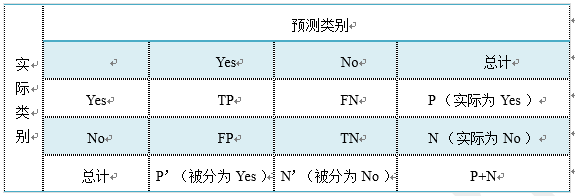
\includegraphics{./img/ch2/2.9/1.png}
\caption{图2-3 术语的混淆矩阵}
\end{figure}

表2-2是这四个术语的混淆矩阵,做以下说明:
1)P=TP+FN表示实际为正例的样本个数。
2)True、False描述的是分类器是否判断正确。
3)Positive、Negative是分类器的分类结果,如果正例计为1、负例计为-1,即positive=1、negative=-1。用1表示True,-1表示False,那么实际的类标=TF*PN,TF为true或false,PN为positive或negative。
4)例如True positives(TP)的实际类标=1*1=1为正例,False
positives(FP)的实际类标=(-1)*1=-1为负例,False
negatives(FN)的实际类标=(-1)*(-1)=1为正例,True
negatives(TN)的实际类标=1*(-1)=-1为负例。

\begin{itemize}
% \tightlist
\item
  \textbf{评价指标}
\end{itemize}

\begin{enumerate}
\def\labelenumi{\arabic{enumi})}
\item
  正确率(accuracy) 正确率是我们最常见的评价指标,accuracy =
  (TP+TN)/(P+N),正确率是被分对的样本数在所有样本数中的占比,通常来说,正确率越高,分类器越好。
\item
  错误率(error rate)
  错误率则与正确率相反,描述被分类器错分的比例,error rate =
  (FP+FN)/(P+N),对某一个实例来说,分对与分错是互斥事件,所以accuracy =1
  - error rate。
\item
  灵敏度(sensitivity) sensitivity =
  TP/P,表示的是所有正例中被分对的比例,衡量了分类器对正例的识别能力。
\item
  特异性(specificity) specificity =
  TN/N,表示的是所有负例中被分对的比例,衡量了分类器对负例的识别能力。
\item
  精度(precision)
  precision=TP/(TP+FP),精度是精确性的度量,表示被分为正例的示例中实际为正例的比例。
\item
  召回率(recall)
  召回率是覆盖面的度量,度量有多个正例被分为正例,recall=TP/(TP+FN)=TP/P=sensitivity,可以看到召回率与灵敏度是一样的。
\item
  其他评价指标 计算速度:分类器训练和预测需要的时间;
  鲁棒性:处理缺失值和异常值的能力; 可扩展性:处理大数据集的能力;
  可解释性:分类器的预测标准的可理解性,像决策树产生的规则就是很容易理解的,而神经网络的一堆参数就不好理解,我们只好把它看成一个黑盒子。
\item
  精度和召回率反映了分类器分类性能的两个方面。如果综合考虑查准率与查全率,可以得到新的评价指标F1-score,也称为综合分类率:$F1=\frac{2 \times precision \times recall}{precision + recall}​$。

\begin{verbatim}
为了综合多个类别的分类情况,评测系统整体性能,经常采用的还有微平均F1(micro-averaging)和宏平均F1(macro-averaging )两种指标。

(1)宏平均F1与微平均F1是以两种不同的平均方式求的全局F1指标。

(2)宏平均F1的计算方法先对每个类别单独计算F1值,再取这些F1值的算术平均值作为全局指标。

(3)微平均F1的计算方法是先累加计算各个类别的a、b、c、d的值,再由这些值求出F1值。

(4)由两种平均F1的计算方式不难看出,宏平均F1平等对待每一个类别,所以它的值主要受到稀有类别的影响,而微平均F1平等考虑文档集中的每一个文档,所以它的值受到常见类别的影响比较大。
\end{verbatim}
\end{enumerate}

\begin{itemize}
\item
  \textbf{ROC曲线和PR曲线}

\begin{verbatim}
如图2-3,ROC曲线是(Receiver Operating Characteristic Curve,受试者工作特征曲线)的简称,是以灵敏度(真阳性率)为纵坐标,以1减去特异性(假阳性率)为横坐标绘制的性能评价曲线。可以将不同模型对同一数据集的ROC曲线绘制在同一笛卡尔坐标系中,ROC曲线越靠近左上角,说明其对应模型越可靠。也可以通过ROC曲线下面的面积(Area Under Curve, AUC)来评价模型,AUC越大,模型越可靠。
\end{verbatim}
\end{itemize}

\begin{figure}
\centering
% 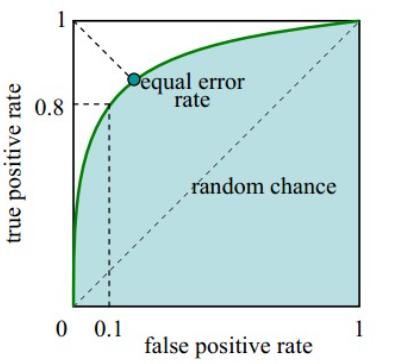
\includegraphics{./img/ch2/2.7.3.png}
\caption{}
\end{figure}

​ 图2-3 ROC曲线

​ PR曲线是Precision Recall
Curve的简称,描述的是precision和recall之间的关系,以recall为横坐标,precision为纵坐标绘制的曲线。该曲线的所对应的面积AUC实际上是目标检测中常用的评价指标平均精度(Average
Precision, AP)。AP越高,说明模型性能越好。

\subsection{2.8.3
正确率能很好的评估分类算法吗}\label{ux6b63ux786eux7387ux80fdux5f88ux597dux7684ux8bc4ux4f30ux5206ux7c7bux7b97ux6cd5ux5417}

​
不同算法有不同特点,在不同数据集上有不同的表现效果,根据特定的任务选择不同的算法。如何评价分类算法的好坏,要做具体任务具体分析。对于决策树,主要用正确率去评估,但是其他算法,只用正确率能很好的评估吗?
​ 答案是否定的。 ​
正确率确实是一个很直观很好的评价指标,但是有时候正确率高并不能完全代表一个算法就好。比如对某个地区进行地震预测,地震分类属性分为0:不发生地震、1发生地震。我们都知道,不发生的概率是极大的,对于分类器而言,如果分类器不加思考,对每一个测试样例的类别都划分为0,达到99\%的正确率,但是,问题来了,如果真的发生地震时,这个分类器毫无察觉,那带来的后果将是巨大的。很显然,99\%正确率的分类器并不是我们想要的。出现这种现象的原因主要是数据分布不均衡,类别为1的数据太少,错分了类别1但达到了很高的正确率缺忽视了研究者本身最为关注的情况。

\subsection{什么样的分类器是最好的}\label{ux4ec0ux4e48ux6837ux7684ux5206ux7c7bux5668ux662fux6700ux597dux7684}

​ 对某一个任务,某个具体的分类器不可能同时满足或提高所有上面介绍的指标。
​
如果一个分类器能正确分对所有的实例,那么各项指标都已经达到最优,但这样的分类器往往不存在。比如之前说的地震预测,既然不能百分百预测地震的发生,但实际情况中能容忍一定程度的误报。假设在1000次预测中,共有5次预测发生了地震,真实情况中有一次发生了地震,其他4次则为误报。正确率由原来的999/1000=99.9下降为996/1000=99.6。召回率由0/1=0\%上升为1/1=100\%。对此解释为,虽然预测失误了4次,但真的地震发生前,分类器能预测对,没有错过,这样的分类器实际意义更为重大,正是我们想要的。在这种情况下,在一定正确率前提下,要求分类器的召回率尽量高。

\section{2.9 逻辑回归}\label{ux903bux8f91ux56deux5f52}

\subsection{2.9.1 回归划分}\label{ux56deux5f52ux5212ux5206}

广义线性模型家族里,依据因变量不同,可以有如下划分:

(1)如果是连续的,就是多重线性回归。

(2)如果是二项分布,就是逻辑回归。

(3)如果是泊松(Poisson)分布,就是泊松回归。

(4)如果是负二项分布,就是负二项回归。

(5)逻辑回归的因变量可以是二分类的,也可以是多分类的,但是二分类的更为常用,也更加容易解释。所以实际中最常用的就是二分类的逻辑回归。

\subsection{逻辑回归适用性}\label{ux903bux8f91ux56deux5f52ux9002ux7528ux6027}

逻辑回归可用于以下几个方面:

(1)用于概率预测。用于可能性预测时,得到的结果有可比性。比如根据模型进而预测在不同的自变量情况下,发生某病或某种情况的概率有多大。

(2)用于分类。实际上跟预测有些类似,也是根据模型,判断某人属于某病或属于某种情况的概率有多大,也就是看一下这个人有多大的可能性是属于某病。进行分类时,仅需要设定一个阈值即可,可能性高于阈值是一类,低于阈值是另一类。

(3)寻找危险因素。寻找某一疾病的危险因素等。

(4)仅能用于线性问题。只有当目标和特征是线性关系时,才能用逻辑回归。在应用逻辑回归时注意两点:一是当知道模型是非线性时,不适用逻辑回归;二是当使用逻辑回归时,应注意选择和目标为线性关系的特征。

(5)各特征之间不需要满足条件独立假设,但各个特征的贡献独立计算。

\subsection{生成模型和判别模型的区别}\label{ux751fux6210ux6a21ux578bux548cux5224ux522bux6a21ux578bux7684ux533aux522b}

生成模型:由数据学习联合概率密度分布P(X,Y),然后求出条件概率分布P(Y\textbar{}X)作为预测的模型,即生成模型:P(Y\textbar{}X)=
P(X,Y)/
P(X)(贝叶斯概率)。基本思想是首先建立样本的联合概率概率密度模型P(X,Y),然后再得到后验概率P(Y\textbar{}X),再利用它进行分类。典型的生成模型有朴素贝叶斯,隐马尔科夫模型等

判别模型:由数据直接学习决策函数Y=f(X)或者条件概率分布P(Y\textbar{}X)作为预测的模型,即判别模型。基本思想是有限样本条件下建立判别函数,不考虑样本的产生模型,直接研究预测模型。典型的判别模型包括k近邻,感知级,决策树,支持向量机等。这些模型的特点都是输入属性X可以直接得到后验概率P(Y\textbar{}X),输出条件概率最大的作为最终的类别(对于二分类任务来说,实际得到一个score,当score大于threshold时则为正类,否则为负类)。

举例:

判别式模型举例:要确定一个羊是山羊还是绵羊,用判别模型的方法是从历史数据中学习到模型,然后通过提取这只羊的特征来预测出这只羊是山羊的概率,是绵羊的概率。

生成式模型举例:利用生成模型是根据山羊的特征首先学习出一个山羊的模型,然后根据绵羊的特征学习出一个绵羊的模型,然后从这只羊中提取特征,放到山羊模型中看概率是多少,在放到绵羊模型中看概率是多少,哪个大就是哪个。

联系和区别:

\begin{verbatim}
生成方法的特点:上面说到,生成方法学习联合概率密度分布P(X,Y),所以就可以从统计的角度表示数据的分布情况,能够反映同类数据本身的相似度。但它不关心到底划分各类的那个分类边界在哪。生成方法可以还原出联合概率分布P(Y,X),而判别方法不能。生成方法的学习收敛速度更快,即当样本容量增加的时候,学到的模型可以更快的收敛于真实模型,当存在隐变量时,仍可以用生成方法学习。此时判别方法就不能用。

判别方法的特点:判别方法直接学习的是决策函数Y=f(X)或者条件概率分布P(Y|X)。不能反映训练数据本身的特性。但它寻找不同类别之间的最优分类面,反映的是异类数据之间的差异。直接面对预测,往往学习的准确率更高。由于直接学习P(Y|X)或P(X),可以对数据进行各种程度上的抽象、定义特征并使用特征,因此可以简化学习问题。
\end{verbatim}

​ 最后,由生成模型可以得到判别模型,但由判别模型得不到生成模型。

\subsection{逻辑回归与朴素贝叶斯有什么区别}\label{ux903bux8f91ux56deux5f52ux4e0eux6734ux7d20ux8d1dux53f6ux65afux6709ux4ec0ux4e48ux533aux522b}

逻辑回归与朴素贝叶斯区别有以下几个方面:

(1)逻辑回归是判别模型,
朴素贝叶斯是生成模型,所以生成和判别的所有区别它们都有。

(2)朴素贝叶斯属于贝叶斯,逻辑回归是最大似然,两种概率哲学间的区别。

(3)朴素贝叶斯需要条件独立假设。

(4)逻辑回归需要求特征参数间是线性的。

\subsection{线性回归与逻辑回归的区别}\label{ux7ebfux6027ux56deux5f52ux4e0eux903bux8f91ux56deux5f52ux7684ux533aux522b}

线性回归与逻辑回归的区别如下描述:

(1)线性回归的样本的输出,都是连续值,$y \in (-\infty ,+\infty )$,而逻辑回归中
$y \in (0,1)$,只能取0和1。

(2)对于拟合函数也有本质上的差别:

​
线性回归:$f(x)=\theta ^{T}x=\theta _{1}x _{1}+\theta _{2}x _{2}+...+\theta _{n}x _{n}$

​
逻辑回归:$f(x)=P(y=1|x;\theta )=g(\theta ^{T}x)$,其中,$g(z)=\frac{1}{1+e^{-z}}$

​
可以看出,线性回归的拟合函数,是对f(x)的输出变量y的拟合,而逻辑回归的拟合函数是对为1类样本的概率的拟合。

​ 那么,为什么要以1类样本的概率进行拟合呢,为什么可以这样拟合呢?

​ $\theta ^{T}x=0$就相当于是1类和0类的决策边界:

​
当$\theta ^{T}x>0$,则$y>0.5$;
若$\theta ^{T}x\rightarrow +\infty $,则
$y\rightarrow  1 $,即y为1类;

​
当$\theta ^{T}x<0$,则$y<0.5$;
若$\theta ^{T}x\rightarrow -\infty$ ,则$y\rightarrow  0 $,即y为0类;

这个时候就能看出区别,在线性回归中$\theta ^{T}x$为预测值的拟合函数;而在逻辑回归中$\theta ^{T}x$为决策边界。下表2-3为线性回归和逻辑回归的区别。

​ 表2-3 线性回归和逻辑回归的区别

\begin{longtable}[]{ ccc }
%\toprule
& 线性回归 & 逻辑回归\tabularnewline
%\midrule
%\endhead
目的 & 预测 & 分类\tabularnewline
$y^{(i)}$ & 未知 & (0,1)\tabularnewline
函数 & 拟合函数 & 预测函数\tabularnewline
参数计算方式 & 最小二乘法 & 极大似然估计\tabularnewline
% \bottomrule
\end{longtable}

下面具体解释一下:

\begin{enumerate}
\def\labelenumi{\arabic{enumi}.}
% \tightlist
\item
  拟合函数和预测函数什么关系呢?简单来说就是将拟合函数做了一个逻辑函数的转换,转换后使得$y^{(i)} \in (0,1)$;
\item
  最小二乘和最大似然估计可以相互替代吗?回答当然是不行了。我们来看看两者依仗的原理:最大似然估计是计算使得数据出现的可能性最大的参数,依仗的自然是Probability。而最小二乘是计算误差损失。
\end{enumerate}

\section{2.10 代价函数}\label{ux4ee3ux4ef7ux51fdux6570}

\subsection{2.10.1
为什么需要代价函数}\label{ux4e3aux4ec0ux4e48ux9700ux8981ux4ee3ux4ef7ux51fdux6570}

\begin{enumerate}
\def\labelenumi{\arabic{enumi}.}
% \tightlist
\item
  为了得到训练逻辑回归模型的参数,需要一个代价函数,通过训练代价函数来得到参数。
\item
  用于找到最优解的目的函数。
\end{enumerate}

\subsection{代价函数作用原理}\label{ux4ee3ux4ef7ux51fdux6570ux4f5cux7528ux539fux7406}

​
在回归问题中,通过代价函数来求解最优解,常用的是平方误差代价函数。假设函数图像如图2-4所示,当参数发生变化时,假设函数状态也会随着变化。

\begin{figure}
\centering
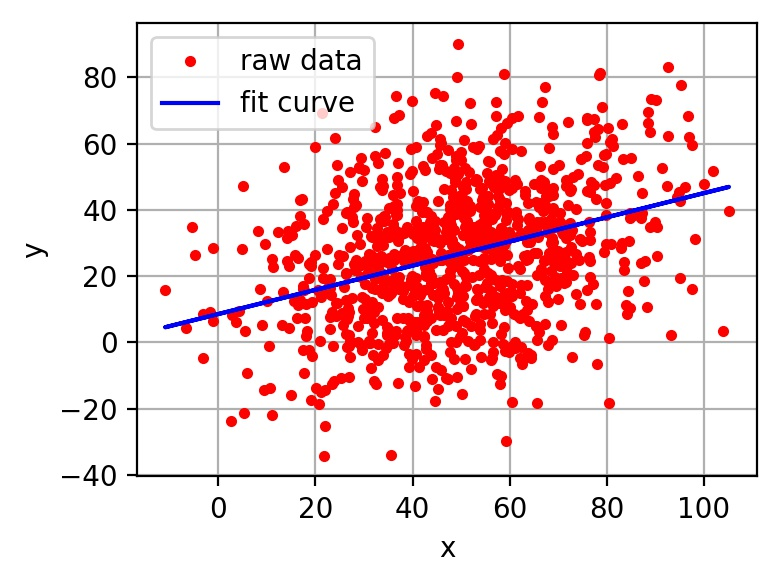
\includegraphics{./img/ch2/2.16/1.jpg}
\caption{}
\end{figure}

​ 图2-4 $h(x) = A + Bx$函数示意图

​
想要拟合图中的离散点,我们需要尽可能找到最优的$A$和$B$来使这条直线更能代表所有数据。如何找到最优解呢,这就需要使用代价函数来求解,以平方误差代价函数为例,假设函数为$h(x)=\theta_0x$。
​
\textbf{平方误差代价函数的主要思想}就是将实际数据给出的值与拟合出的线的对应值做差,求出拟合出的直线与实际的差距。在实际应用中,为了避免因个别极端数据产生的影响,采用类似方差再取二分之一的方式来减小个别数据的影响。因此,引出代价函数:

\[
J(\theta_0, \theta_1) = \frac{1}{m}\sum_{i=1}^m(h(x^{(i)})-y^{(i)})^2
\]

​
\textbf{最优解即为代价函数的最小值}$\min J(\theta_0, \theta_1)$。如果是1个参数,代价函数一般通过二维曲线便可直观看出。如果是2个参数,代价函数通过三维图像可看出效果,参数越多,越复杂。
当参数为2个时,代价函数是三维图像,如下图2-5所示。

\begin{figure}
\centering
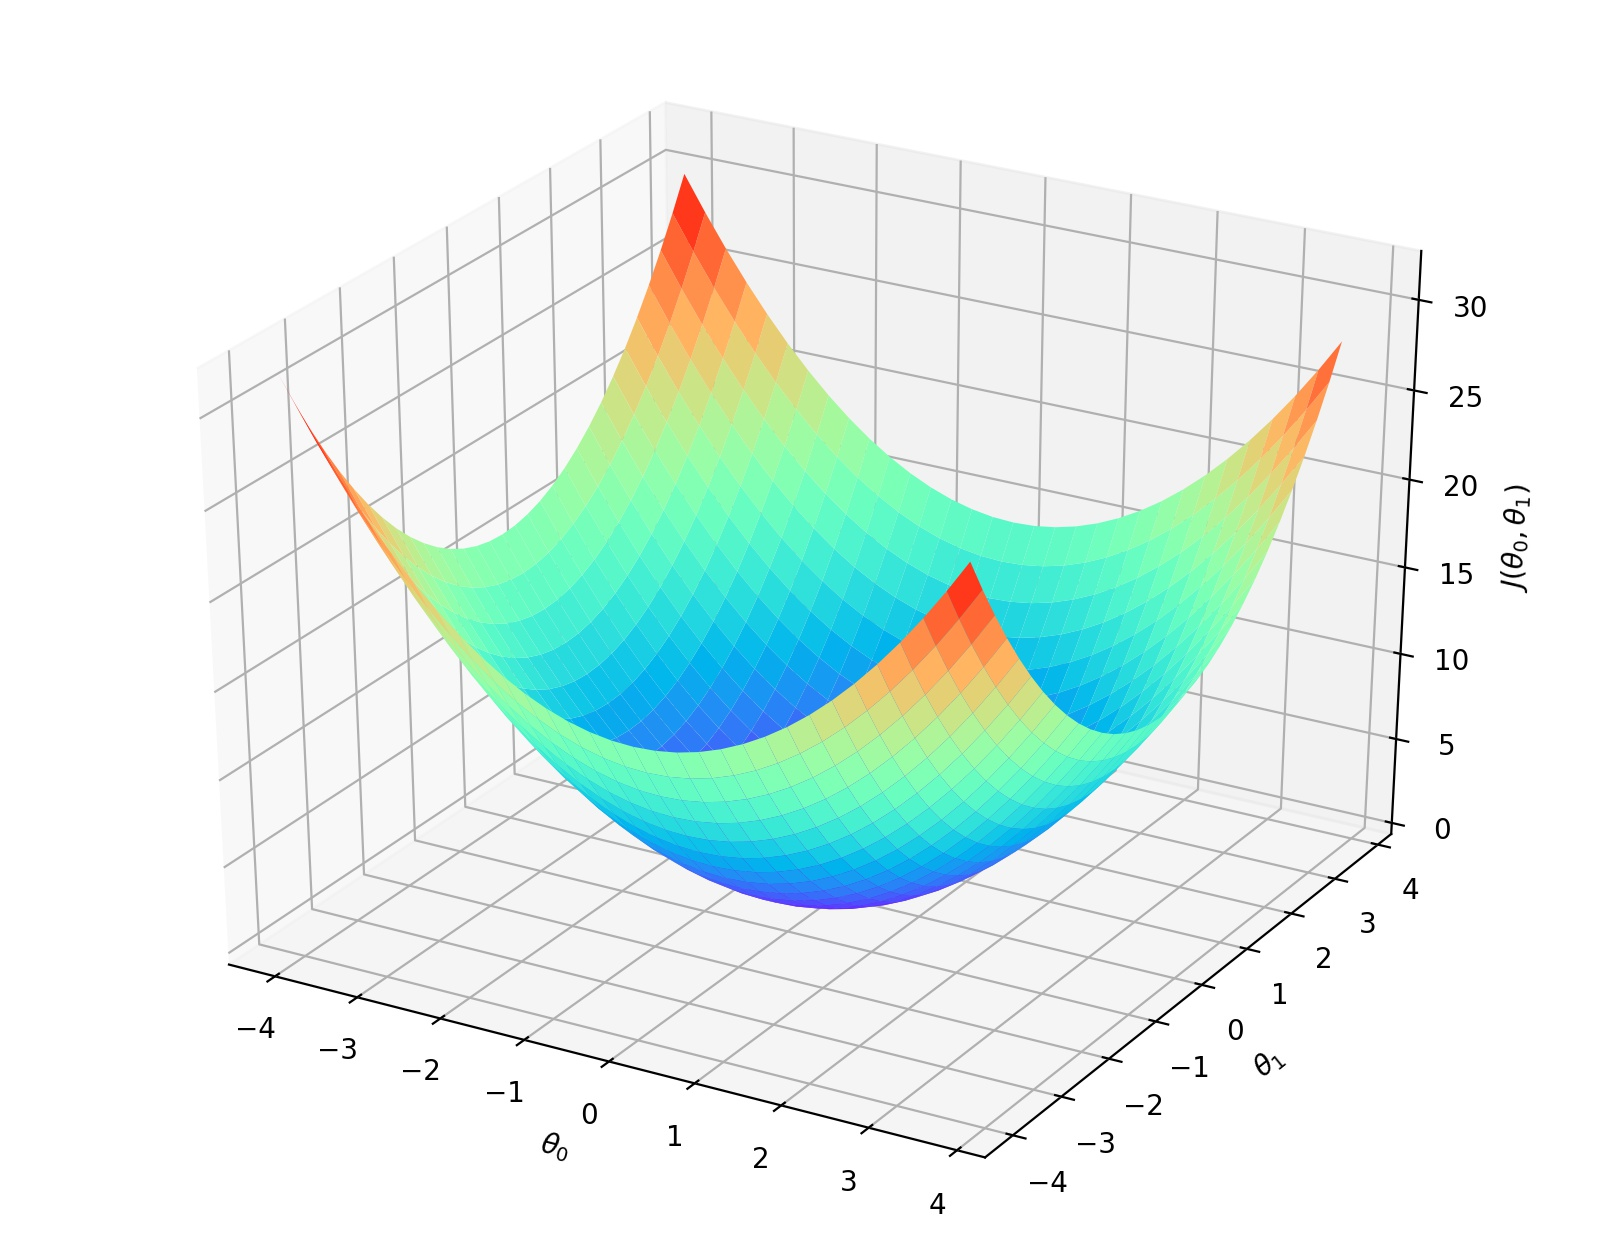
\includegraphics{./img/ch2/2.16/2.jpg}
\caption{}
\end{figure}

​ 图2-5 代价函数三维图像

\subsection{为什么代价函数要非负}\label{ux4e3aux4ec0ux4e48ux4ee3ux4ef7ux51fdux6570ux8981ux975eux8d1f}

​
目标函数存在一个下界,在优化过程当中,如果优化算法能够使目标函数不断减小,根据单调有界准则,这个优化算法就能证明是收敛有效的。
​ 只要设计的目标函数有下界,基本上都可以,代价函数非负更为方便。

\subsection{常见代价函数}\label{ux5e38ux89c1ux4ee3ux4ef7ux51fdux6570}

(1)\textbf{二次代价函数(quadratic cost)}: \[
J = \frac{1}{2n}\sum_x\Vert y(x)-a^L(x)\Vert^2
\]

​
其中,$J$表示代价函数,$x$表示样本,$y$表示实际值,$a$表示输出值,$n$表示样本的总数。使用一个样本为例简单说明,此时二次代价函数为:
\[
J = \frac{(y-a)^2}{2}
\] ​ 假如使用梯度下降法(Gradient
descent)来调整权值参数的大小,权值$w$和偏置$b$的梯度推导如下: \[
\frac{\partial J}{\partial w}=(y-a)\sigma'(z)x\;,
\frac{\partial J}{\partial b}=(y-a)\sigma'(z)
\]
其中,$z​$表示神经元的输入,$\sigma​$表示激活函数。权值$w​$和偏置$b​$的梯度跟激活函数的梯度成正比,激活函数的梯度越大,权值$w​$和偏置$b​$的大小调整得越快,训练收敛得就越快。

\emph{注}:神经网络常用的激活函数为sigmoid函数,该函数的曲线如下图2-6所示:

\begin{figure}
\centering
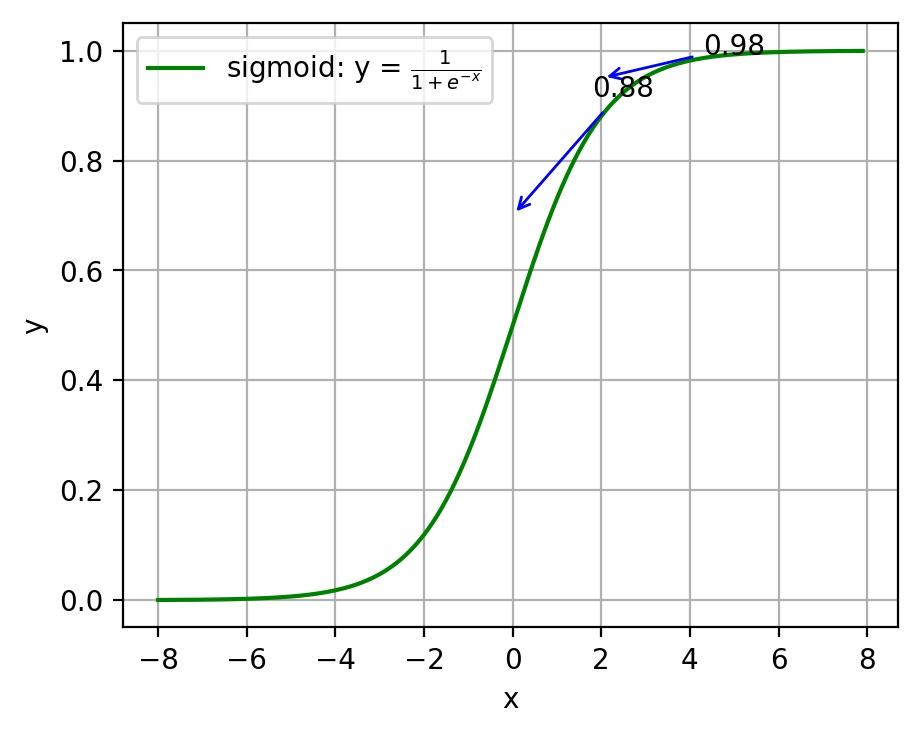
\includegraphics{./img/ch2/2.18/1.jpg}
\caption{}
\end{figure}

​ 图2-6 sigmoid函数曲线

如上图所示,对0.88和0.98两个点进行比较: ​
假设目标是收敛到1.0。0.88离目标1.0比较远,梯度比较大,权值调整比较大。0.98离目标1.0比较近,梯度比较小,权值调整比较小。调整方案合理。
​
假如目标是收敛到0。0.88离目标0比较近,梯度比较大,权值调整比较大。0.98离目标0比较远,梯度比较小,权值调整比较小。调整方案不合理。
​ 原因:在使用sigmoid函数的情况下,
初始的代价(误差)越大,导致训练越慢。

(2)\textbf{交叉熵代价函数(cross-entropy)}: \[
J = -\frac{1}{n}\sum_x[y\ln a + (1-y)\ln{(1-a)}]
\]

其中,$J$表示代价函数,$x$表示样本,$y$表示实际值,$a$表示输出值,$n$表示样本的总数。
权值$w$和偏置$b​$的梯度推导如下: \[
\frac{\partial J}{\partial w_j}=\frac{1}{n}\sum_{x}x_j(\sigma{(z)}-y)\;,
\frac{\partial J}{\partial b}=\frac{1}{n}\sum_{x}(\sigma{(z)}-y)
\]

当误差越大时,梯度就越大,权值$w$和偏置$b$调整就越快,训练的速度也就越快。
\textbf{二次代价函数适合输出神经元是线性的情况,交叉熵代价函数适合输出神经元是S型函数的情况。}

(3)\textbf{对数似然代价函数(log-likelihood cost)}:
对数似然函数常用来作为softmax回归的代价函数。深度学习中普遍的做法是将softmax作为最后一层,此时常用的代价函数是对数似然代价函数。
对数似然代价函数与softmax的组合和交叉熵与sigmoid函数的组合非常相似。对数似然代价函数在二分类时可以化简为交叉熵代价函数的形式。
在tensorflow中:
与sigmoid搭配使用的交叉熵函数:\texttt{tf.nn.sigmoid\_cross\_entropy\_with\_logits()}。
与softmax搭配使用的交叉熵函数:\texttt{tf.nn.softmax\_cross\_entropy\_with\_logits()}。
在pytorch中:
与sigmoid搭配使用的交叉熵函数:\texttt{torch.nn.BCEWithLogitsLoss()}。
与softmax搭配使用的交叉熵函数:\texttt{torch.nn.CrossEntropyLoss()}。

对数似然函数:

​
我们将似然函数作为机器学习模型的损失函数,并且用在分类问题中。这时似然函数是直接作用于模型的输出的(损失函数就是为了衡量当前参数下model的预测值predict距离真实值label的大小,所以似然函数用作损失函数时当然也是为了完成该任务),所以对于似然函数来说,这里的样本集就成了label集(而不是机器学习意义上的样本集X了),这里的参数也不是机器学习model
的参数,而是predict值。

其实作为损失函数的似然函数并不关心你当前的机器学习model的参数是怎样的,毕竟它此时所接收的输入只有两部分:\textbf{1、predict。2、label
。3、分布模型(predict服从的分布)}。

显然这里的label就是似然函数的观测值,即样本集。\textbf{而它眼里的模型,当然就是predict这个随机变量所服从的概率分布模型。它的目的,就是衡量predict背后的模型对于当前观测值的解释程度。而每个样本的predict值,恰恰就是它所服从的分布模型的参数。}

比如此时我们的机器学习任务是一个4个类别的分类任务,机器学习model的输出就是当前样本X下的每个类别的概率,如predict={[}0.1,
0.1, 0.7, 0.1{]},而该样本的标签是类别3,表示成向量就是label={[}0, 0, 1,
0{]}。那么label={[}0, 0, 1,
0{]}就是似然函数眼里的样本,然后我们可以假设predict这个随机变量背后的模型是\textbf{单次观测下的多项式分布},(\textbf{因为softmax本身是基于多项式分布的})。

回顾:

伯努利分布,也叫做(0,1)分布,贝努利分布可以看成是将一枚硬币(只有正反两个面,代表两个类别)向上扔出,出现某个面(类别)的概率情况,因此其概率密度函数为:

\[
f(x)=p^x(1-p)^{1-x}=
\begin{cases}
p,& x=1\\
q,& x=0
\end{cases}
\]
这是理解似然函数做损失函数的关键!另外,贝努利分布的模型参数就是其中一个类别的发生概率。

而二项分布呢,就是将贝努利实验重复n次(各次实验之间是相互独立的)。

而多项式分布呢,就是将二项分布推广到多个面(类别)。

\textbf{所以,单次观测下的多项式分布就是贝努利分布的多类推广!即:} \[
f_{mulit}(x;p)=\prod_{i=1}^C p_{i}^{xi}
\]
其中,C代表类别数。p代表向量形式的模型参数,即各个类别的发生概率,如p={[}0.1,
0.1, 0.7, 0.1{]},则p1=0.1,
p3=0.7等。即,\textbf{多项式分布的模型参数就是各个类别的发生概率!}x代表\textbf{one-hot形式}的观测值,如x=类别3,则x={[}0,
0, 1, 0{]}。xi代表x的第i个元素,比如x=类别3时,x1=0,x2=0,x3=1,x4=0。

想一下,机器学习model对某个样本的输出,就代表各个类别发生的概率。但是,对于当前\textbf{这一个}样本而言,它肯定只能有\textbf{一个类别},所以这一个样本就可以看成是一次实验(观察),而这次实验(观察)的结果要服从上述各个类别发生的概率,那不就是服从多项式分布嘛!而且是单次观察!各个类别发生的概率predict当然就是这个多项式分布的参数。

\textbf{总结一下,对于多类分类问题,似然函数就是衡量当前这个以predict为参数的单次观测下的多项式分布模型与样本值label之间的似然度。}

所以,根据似然函数的定义,单个样本的似然函数即:

\[
L = f_{mulit}(label;predict)
\] 所以,整个样本集(或者一个batch)的似然函数即: \[
L=\prod_{X}f_{multi}(label;predict)= \prod_{X}\prod_{i=1}^{C}predict(i)^{label(i)}
\] 所以在累乘号前面加上log函数后,就成了所谓的对数似然函数: \[
L=\sum_{X}\sum_{i=1}^{C}label(i)log(predict(i))
\]
而最大化对数似然函数就等效于最小化负对数似然函数,所以前面加个负号就和交叉熵的形式相同的了。

交叉熵定义:对于某种分布的随机变量X\textasciitilde{}p(x),
有一个模型q(x)用于近似p(x)的概率分布,则分布X与模型q之间的交叉熵即:

\[
H(X,q)=-\sum_{x}p(x)logq(x)
\]
这里X的分布模型即样本集label的真实分布模型,这里模型q(x)即想要模拟真实分布模型的机器学习模型。可以说交叉熵是直接衡量两个分布,或者说两个model之间的差异。而似然函数则是解释以model的输出为参数的某分布模型对样本集的解释程度。因此,可以说这两者是``同貌不同源'',但是``殊途同归''啦。

tips:

最大似然估计:

给定一堆数据,假如我们知道它是从某一种分布中随机取出来的,可是我们并不知道这个分布具体的参,即``模型已定,参数未知''。例如,我们知道这个分布是正态分布,但是不知道均值和方差;或者是二项分布,但是不知道均值。最大似然估计(MLE,Maximum
Likelihood
Estimation)就可以用来估计模型的参数。\textbf{MLE的目标是找出一组参数,使得模型产生出观测数据的概率最大。}

\subsection{2.10.5
为什么用交叉熵代替二次代价函数}\label{ux4e3aux4ec0ux4e48ux7528ux4ea4ux53c9ux71b5ux4ee3ux66ffux4e8cux6b21ux4ee3ux4ef7ux51fdux6570}

(1)\textbf{为什么不用二次方代价函数}
由上一节可知,权值$w$和偏置$b$的偏导数为$\frac{\partial J}{\partial w}=(a-y)\sigma'(z)x$,$\frac{\partial J}{\partial b}=(a-y)\sigma'(z)$,
偏导数受激活函数的导数影响,sigmoid函数导数在输出接近0和1时非常小,会导致一些实例在刚开始训练时学习得非常慢。

(2)\textbf{为什么要用交叉熵}
交叉熵函数权值$w$和偏置$b$的梯度推导为: \[
\frac{\partial J}{\partial w_j}=\frac{1}{n}\sum_{x}x_j(\sigma{(z)}-y)\;,
\frac{\partial J}{\partial b}=\frac{1}{n}\sum_{x}(\sigma{(z)}-y)
\]

由以上公式可知,权重学习的速度受到$\sigma{(z)}-y$影响,更大的误差,就有更快的学习速度,避免了二次代价函数方程中因$\sigma'{(z)}$导致的学习缓慢的情况。

\section{2.11 损失函数}\label{ux635fux5931ux51fdux6570}

\subsection{2.11.1
什么是损失函数}\label{ux4ec0ux4e48ux662fux635fux5931ux51fdux6570}

​ 损失函数(Loss
Function)又叫做误差函数,用来衡量算法的运行情况,估量模型的预测值与真实值的不一致程度,是一个非负实值函数,通常使用$
L(Y,
f(x))​$来表示。损失函数越小,模型的鲁棒性就越好。损失函数是经验风险函数的核心部分,也是结构风险函数重要组成部分。

\subsection{2.11.2
常见的损失函数}\label{ux5e38ux89c1ux7684ux635fux5931ux51fdux6570}

​
机器学习通过对算法中的目标函数进行不断求解优化,得到最终想要的结果。分类和回归问题中,通常使用损失函数或代价函数作为目标函数。
​
损失函数用来评价预测值和真实值不一样的程度。通常损失函数越好,模型的性能也越好。
​
损失函数可分为经验风险损失函数和结构风险损失函数。经验风险损失函数指预测结果和实际结果的差别,结构风险损失函数是在经验风险损失函数上加上正则项。
​ 下面介绍常用的损失函数:

(1)\textbf{0-1损失函数}
如果预测值和目标值相等,值为0,如果不相等,值为1。 \[
L(Y, f(x)) =
\begin{cases}
1,& Y\ne f(x)\\
0,& Y = f(x)
\end{cases}
\]

一般的在实际使用中,相等的条件过于严格,可适当放宽条件:

\[
L(Y, f(x)) =
\begin{cases}
1,& |Y-f(x)|\geqslant T\\
0,& |Y-f(x)|< T
\end{cases}
\]

(2)\textbf{绝对值损失函数} 和0-1损失函数相似,绝对值损失函数表示为:
\[
L(Y, f(x)) = |Y-f(x)|​
\]

(3)\textbf{平方损失函数} \[
L(Y, f(x)) = \sum_N{(Y-f(x))}^2
\]

这点可从最小二乘法和欧几里得距离角度理解。最小二乘法的原理是,最优拟合曲线应该使所有点到回归直线的距离和最小。

(4)\textbf{对数损失函数} \[
L(Y, P(Y|X)) = -\log{P(Y|X)}=-\frac{1}{N}\sum_{i=1}^N\sum_{j=1}^M y_{ij}log(p_{ij})
\]

​ 其中, Y 为输出变量, X为输入变量, L 为损失函数. N为输入样本量,
M为可能的类别数, $y_{ij}$ 是一个二值指标, 表示类别 j 是否是输入实例 xi
的真实类别. $p_{ij}$ 为模型或分类器预测输入实例 xi 属于类别 j 的概率.

常见的逻辑回归使用的就是对数损失函数,有很多人认为逻辑回归的损失函数是平方损失,其实不然。逻辑回归它假设样本服从伯努利分布(0-1分布),进而求得满足该分布的似然函数,接着取对数求极值等。逻辑回归推导出的经验风险函数是最小化负的似然函数,从损失函数的角度看,就是对数损失函数。形式上等价于二分类的交叉熵损失函数。

(6)\textbf{指数损失函数} 指数损失函数的标准形式为: \[
L(Y, f(x)) = \exp(-Yf(x))
\]

例如AdaBoost就是以指数损失函数为损失函数。

(7)\textbf{Hinge损失函数} Hinge损失函数的标准形式如下: \[
L(y) = \max{(0, 1-ty)}
\]

统一的形式: \[
L(Y, f(x)) = \max{(0, Yf(x))}
\]

其中y是预测值,范围为(-1,1),t为目标值,其为-1或1。

在线性支持向量机中,最优化问题可等价于

\[
\underset{\min}{w,b}\sum_{i=1}^N (1-y_i(wx_i+b))+\lambda\Vert w\Vert ^2
\]

上式相似于下式

\[
\frac{1}{m}\sum_{i=1}^{N}l(wx_i+by_i) + \Vert w\Vert ^2
\]

其中$l(wx_i+by_i)$是Hinge损失函数,$\Vert w\Vert ^2$可看做为正则化项。

\subsection{2.11.3
逻辑回归为什么使用对数损失函数}\label{ux903bux8f91ux56deux5f52ux4e3aux4ec0ux4e48ux4f7fux7528ux5bf9ux6570ux635fux5931ux51fdux6570}

假设逻辑回归模型 \[
P(y=1|x;\theta)=\frac{1}{1+e^{-\theta^{T}x}}
\] 假设逻辑回归模型的概率分布是伯努利分布,其概率质量函数为: \[
P(X=n)=
\begin{cases}
1-p, n=0\\
 p,n=1
\end{cases}
\] 其似然函数为: \[
L(\theta)=\prod_{i=1}^{m}
P(y=1|x_i)^{y_i}P(y=0|x_i)^{1-y_i}
\] 对数似然函数为: \[
\ln L(\theta)=\sum_{i=1}^{m}[y_i\ln{P(y=1|x_i)}+(1-y_i)\ln{P(y=0|x_i)}]\\
  =\sum_{i=1}^m[y_i\ln{P(y=1|x_i)}+(1-y_i)\ln(1-P(y=1|x_i))]
\] 对数函数在单个数据点上的定义为: \[
cost(y,p(y|x))=-y\ln{p(y|x)-(1-y)\ln(1-p(y|x))}
\] 则全局样本损失函数为: \[
cost(y,p(y|x)) = -\sum_{i=1}^m[y_i\ln p(y_i|x_i)+(1-y_i)\ln(1-p(y_i|x_i))]
\]
由此可看出,对数损失函数与极大似然估计的对数似然函数本质上是相同的。所以逻辑回归直接采用对数损失函数。

\subsection{对数损失函数是如何度量损失的}\label{ux5bf9ux6570ux635fux5931ux51fdux6570ux662fux5982ux4f55ux5ea6ux91cfux635fux5931ux7684}

​ 例如,在高斯分布中,我们需要确定均值和标准差。 ​
如何确定这两个参数?最大似然估计是比较常用的方法。最大似然的目标是找到一些参数值,这些参数值对应的分布可以最大化观测到数据的概率。
​
因为需要计算观测到所有数据的全概率,即所有观测到的数据点的联合概率。现考虑如下简化情况:

(1)假设观测到每个数据点的概率和其他数据点的概率是独立的。

(2)取自然对数。 假设观测到单个数据点$x_i(i=1,2,...n)$的概率为: \[
P(x_i;\mu,\sigma)=\frac{1}{\sigma \sqrt{2\pi}}\exp 
        \left( - \frac{(x_i-\mu)^2}{2\sigma^2} \right)
\]

(3)其联合概率为: \[
P(x_1,x_2,...,x_n;\mu,\sigma)=\frac{1}{\sigma \sqrt{2\pi}}\exp 
        \left( - \frac{(x_1-\mu)^2}{2\sigma^2} \right) \\ \times
         \frac{1}{\sigma \sqrt{2\pi}}\exp 
        \left( - \frac{(x_2-\mu)^2}{2\sigma^2} \right) \times ... \times
        \frac{1}{\sigma \sqrt{2\pi}}\exp 
        \left( - \frac{(x_n-\mu)^2}{2\sigma^2} \right)
\] ​ 对上式取自然对数,可得: \[
 \ln(P(x_1,x_2,...x_n;\mu,\sigma))=
        \ln \left(\frac{1}{\sigma \sqrt{2\pi}} \right) 
         - \frac{(x_1-\mu)^2}{2\sigma^2}  \\ +
         \ln \left( \frac{1}{\sigma \sqrt{2\pi}} \right) 
         - \frac{(x_2-\mu)^2}{2\sigma^2} +...+
         \ln \left( \frac{1}{\sigma \sqrt{2\pi}} \right) 
         - \frac{(x_n-\mu)^2}{2\sigma^2}
\] 根据对数定律,上式可以化简为: \[
\ln(P(x_1,x_2,...x_n;\mu,\sigma))=-n\ln(\sigma)-\frac{n}{2} \ln(2\pi)\\
        -\frac{1}{2\sigma^2}[(x_1-\mu)^2+(x_2-\mu)^2+...+(x_n-\mu)^2]
\] 然后求导为: \[
\frac{\partial\ln(P(x_1,x_2,...,x_n;\mu,\sigma))}{\partial\mu}=
                \frac{n}{\sigma^2}[\mu - (x_1+x_2+...+x_n)]
\] ​
上式左半部分为对数损失函数。损失函数越小越好,因此我们令等式左半的对数损失函数为0,可得:
\[
\mu=\frac{x_1+x_2+...+x_n}{n}
\] 同理,可计算$\sigma ​$。

\section{ 梯度下降}\label{ux68afux5ea6ux4e0bux964d}

\subsection{机器学习中为什么需要梯度下降}\label{ux673aux5668ux5b66ux4e60ux4e2dux4e3aux4ec0ux4e48ux9700ux8981ux68afux5ea6ux4e0bux964d}

梯度下降是机器学习中常见优化算法之一,梯度下降法有以下几个作用:

(1)梯度下降是迭代法的一种,可以用于求解最小二乘问题。

(2)在求解机器学习算法的模型参数,即无约束优化问题时,主要有梯度下降法(Gradient
Descent)和最小二乘法。

(3)在求解损失函数的最小值时,可以通过梯度下降法来一步步的迭代求解,得到最小化的损失函数和模型参数值。

(4)如果我们需要求解损失函数的最大值,可通过梯度上升法来迭代。梯度下降法和梯度上升法可相互转换。

(5)在机器学习中,梯度下降法主要有随机梯度下降法和批量梯度下降法。

\subsection{梯度下降法缺点}\label{ux68afux5ea6ux4e0bux964dux6cd5ux7f3aux70b9}

梯度下降法缺点有以下几点:

(1)靠近极小值时收敛速度减慢。

(2)直线搜索时可能会产生一些问题。

(3)可能会``之字形''地下降。

梯度概念也有需注意的地方:

(1)梯度是一个向量,即有方向有大小。

(2)梯度的方向是最大方向导数的方向。

(3)梯度的值是最大方向导数的值。

\subsection{梯度下降法直观理解}\label{ux68afux5ea6ux4e0bux964dux6cd5ux76f4ux89c2ux7406ux89e3}

梯度下降法经典图示如下图2.7所示:

\begin{figure}
\centering
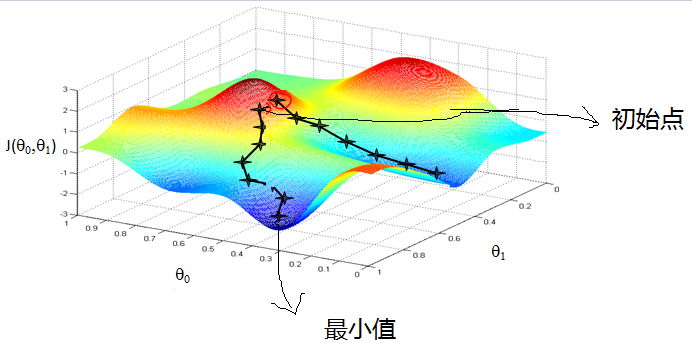
\includegraphics{./img/ch2/2.25/1.png}
\caption{}
\end{figure}

​ 图2.7 梯度下降法经典图示

​
形象化举例,由上图2.7所示,假如最开始,我们在一座大山上的某处位置,因为到处都是陌生的,不知道下山的路,所以只能摸索着根据直觉,走一步算一步,在此过程中,每走到一个位置的时候,都会求解当前位置的梯度,沿着梯度的负方向,也就是当前最陡峭的位置向下走一步,然后继续求解当前位置梯度,向这一步所在位置沿着最陡峭最易下山的位置走一步。不断循环求梯度,就这样一步步地走下去,一直走到我们觉得已经到了山脚。当然这样走下去,有可能我们不能走到山脚,而是到了某一个局部的山势低处。
​
由此,从上面的解释可以看出,梯度下降不一定能够找到全局的最优解,有可能是一个局部的最优解。当然,如果损失函数是凸函数,梯度下降法得到的解就一定是全局最优解。

\textbf{核心思想归纳}:

(1)初始化参数,随机选取取值范围内的任意数;

(2)迭代操作: a)计算当前梯度; b)修改新的变量;
c)计算朝最陡的下坡方向走一步; d)判断是否需要终止,如否,返回a);

(3)得到全局最优解或者接近全局最优解。

\subsection{梯度下降法算法描述}\label{ux68afux5ea6ux4e0bux964dux6cd5ux7b97ux6cd5ux63cfux8ff0}

梯度下降法算法步骤如下:

(1)确定优化模型的假设函数及损失函数。 ​
举例,对于线性回归,假设函数为: \[
  h_\theta(x_1,x_2,...,x_n)=\theta_0+\theta_1x_1+...+\theta_nx_n
\]
其中,$\theta_i,x_i(i=0,1,2,...,n)$分别为模型参数、每个样本的特征值。
对于假设函数,损失函数为: \[
  J(\theta_0,\theta_1,...,\theta_n)=\frac{1}{2m}\sum^{m}_{j=0}(h_\theta (x^{(j)}_0
    ,x^{(j)}_1,...,x^{(j)}_n)-y_j)^2
\]

(2)相关参数初始化。 ​
主要初始化${\theta}_i$、算法迭代步长${\alpha}$、终止距离${\zeta}$ 。初始化时可以根据经验初始化,即${\theta}
$初始化为0,步长${\alpha} $初始化为1。当前步长记为${\varphi}\_i
$。当然,也可随机初始化。

(3)迭代计算。

​ 1)计算当前位置时损失函数的梯度,对${\theta}\_i $,其梯度表示为:
\[
\frac{\partial}{\partial \theta_i}J({\theta}_0,{\theta}_1,...,{\theta}_n)=\frac{1}{2m}\sum^{m}_{j=0}(h_\theta (x^{(j)}_0
    ,x^{(j)}_1,...,x^{(j)}_n)-y_j)^2
\] ​ 2)计算当前位置下降的距离。 \[
{\varphi}_i={\alpha} \frac{\partial}{\partial \theta_i}J({\theta}_0,{\theta}_1,...,{\theta}_n)
\] ​ 3)判断是否终止。 ​
确定是否所有${\theta}_i$梯度下降的距离${\varphi}_i$都小于终止距离${\zeta}$,如果都小于${\zeta}$,则算法终止,当然的值即为最终结果,否则进入下一步。
​ 4)更新所有的${\theta}_i$,更新后的表达式为: \[
{\theta}_i={\theta}_i-\alpha \frac{\partial}{\partial \theta_i}J({\theta}_0,{\theta}_1,...,{\theta}_n)
\] \[
\theta_i=\theta_i - \alpha \frac{1}{m} \sum^{m}_{j=0}(h_\theta (x^{(j)}_0
    ,x^{(j)}_1,...,x^{(j)}_n)-y_j)x^{(j)}_i
\] ​ 5)令上式$x^{(j)}_0=1$,更新完毕后转入1)。 ​
由此,可看出,当前位置的梯度方向由所有样本决定,上式中
$\frac{1}{m}​$、$\alpha \frac{1}{m}​$ 的目的是为了便于理解。

\subsection{如何对梯度下降法进行调优}\label{ux5982ux4f55ux5bf9ux68afux5ea6ux4e0bux964dux6cd5ux8fdbux884cux8c03ux4f18}

实际使用梯度下降法时,各项参数指标不能一步就达到理想状态,对梯度下降法调优主要体现在以下几个方面:

(1)\textbf{算法迭代步长$\alpha$选择。}
在算法参数初始化时,有时根据经验将步长初始化为1。实际取值取决于数据样本。可以从大到小,多取一些值,分别运行算法看迭代效果,如果损失函数在变小,则取值有效。如果取值无效,说明要增大步长。但步长太大,有时会导致迭代速度过快,错过最优解。步长太小,迭代速度慢,算法运行时间长。

(2)\textbf{参数的初始值选择。}
初始值不同,获得的最小值也有可能不同,梯度下降有可能得到的是局部最小值。如果损失函数是凸函数,则一定是最优解。由于有局部最优解的风险,需要多次用不同初始值运行算法,关键损失函数的最小值,选择损失函数最小化的初值。

(3)\textbf{标准化处理。}
由于样本不同,特征取值范围也不同,导致迭代速度慢。为了减少特征取值的影响,可对特征数据标准化,使新期望为0,新方差为1,可节省算法运行时间。

\subsection{随机梯度和批量梯度区别}\label{ux968fux673aux68afux5ea6ux548cux6279ux91cfux68afux5ea6ux533aux522b}

​
随机梯度下降(SGD)和批量梯度下降(BGD)是两种主要梯度下降法,其目的是增加某些限制来加速运算求解。
下面通过介绍两种梯度下降法的求解思路,对其进行比较。 假设函数为: \[
h_\theta (x_0,x_1,...,x_3) = \theta_0 x_0 + \theta_1 x_1 + ... + \theta_n x_n
\] 损失函数为: \[
J(\theta_0, \theta_1, ... , \theta_n) = 
            \frac{1}{2m} \sum^{m}_{j=0}(h_\theta (x^{j}_0
    ,x^{j}_1,...,x^{j}_n)-y^j)^2
\] 其中,$m​$为样本个数,$j​$为参数个数。

1、 \textbf{批量梯度下降的求解思路如下:} a) 得到每个$
\theta ​$对应的梯度: \[
\frac{\partial}{\partial \theta_i}J({\theta}_0,{\theta}_1,...,{\theta}_n)=\frac{1}{m}\sum^{m}_{j=0}(h_\theta (x^{j}_0
    ,x^{j}_1,...,x^{j}_n)-y^j)x^{j}_i
\] b) 由于是求最小化风险函数,所以按每个参数 $ \theta ​$
的梯度负方向更新 $ \theta\_i ​$ : \[
\theta_i=\theta_i - \frac{1}{m} \sum^{m}_{j=0}(h_\theta (x^{j}_0
    ,x^{j}_1,...,x^{j}_n)-y^j)x^{j}_i
\] c)
从上式可以注意到,它得到的虽然是一个全局最优解,但每迭代一步,都要用到训练集所有的数据,如果样本数据很大,这种方法迭代速度就很慢。
相比而言,随机梯度下降可避免这种问题。

2、\textbf{随机梯度下降的求解思路如下:} a)
相比批量梯度下降对应所有的训练样本,随机梯度下降法中损失函数对应的是训练集中每个样本的粒度。
损失函数可以写成如下这种形式, \[
J(\theta_0, \theta_1, ... , \theta_n) = 
            \frac{1}{m} \sum^{m}_{j=0}(y^j - h_\theta (x^{j}_0
            ,x^{j}_1,...,x^{j}_n))^2 = 
            \frac{1}{m} \sum^{m}_{j=0} cost(\theta,(x^j,y^j))
\] b)对每个参数 $ \theta​$ 按梯度方向更新 $ \theta​$: \[
\theta_i = \theta_i + (y^j - h_\theta (x^{j}_0, x^{j}_1, ... ,x^{j}_n))
\] c) 随机梯度下降是通过每个样本来迭代更新一次。
随机梯度下降伴随的一个问题是噪音较批量梯度下降要多,使得随机梯度下降并不是每次迭代都向着整体最优化方向。

\textbf{小结:}
随机梯度下降法、批量梯度下降法相对来说都比较极端,简单对比如下:

\begin{longtable}[]{ cl }
%\toprule
\begin{minipage}[b]{0.17\columnwidth}\centering\strut
方法\strut
\end{minipage} & \begin{minipage}[b]{0.78\columnwidth}\raggedright\strut
特点\strut
\end{minipage}\tabularnewline
%\midrule
%\endhead
\begin{minipage}[t]{0.17\columnwidth}\centering\strut
批量梯度下降\strut
\end{minipage} & \begin{minipage}[t]{0.78\columnwidth}\raggedright\strut
a)采用所有数据来梯度下降。b)批量梯度下降法在样本量很大的时候,训练速度慢。\strut
\end{minipage}\tabularnewline
\begin{minipage}[t]{0.17\columnwidth}\centering\strut
随机梯度下降\strut
\end{minipage} & \begin{minipage}[t]{0.78\columnwidth}\raggedright\strut
a)随机梯度下降用一个样本来梯度下降。b)训练速度很快。c)随机梯度下降法仅仅用一个样本决定梯度方向,导致解有可能不是全局最优。d)收敛速度来说,随机梯度下降法一次迭代一个样本,导致迭代方向变化很大,不能很快的收敛到局部最优解。\strut
\end{minipage}\tabularnewline
% \bottomrule
\end{longtable}

下面介绍能结合两种方法优点的小批量梯度下降法。

3、 \textbf{小批量(Mini-Batch)梯度下降的求解思路如下}
对于总数为$m$个样本的数据,根据样本的数据,选取其中的$n(1< n< m)$个子样本来迭代。其参数$\theta$按梯度方向更新$\theta_i$公式如下:
\[
\theta_i = \theta_i - \alpha \sum^{t+n-1}_{j=t}
        ( h_\theta (x^{j}_{0}, x^{j}_{1}, ... , x^{j}_{n} ) - y^j ) x^{j}_{i}
\]

\subsection{2.12.7
各种梯度下降法性能比较}\label{ux5404ux79cdux68afux5ea6ux4e0bux964dux6cd5ux6027ux80fdux6bd4ux8f83}

​
下表简单对比随机梯度下降(SGD)、批量梯度下降(BGD)、小批量梯度下降(Mini-batch
GD)、和Online GD的区别:

\begin{longtable}[]{ ccccc }
%\toprule
& BGD & SGD & Mini-batch GD & Online GD\tabularnewline
%\midrule
%\endhead
训练集 & 固定 & 固定 & 固定 & 实时更新\tabularnewline
单次迭代样本数 & 整个训练集 & 单个样本 & 训练集的子集 &
根据具体算法定\tabularnewline
算法复杂度 & 高 & 低 & 一般 & 低\tabularnewline
时效性 & 低 & 一般 & 一般 & 高\tabularnewline
收敛性 & 稳定 & 不稳定 & 较稳定 & 不稳定\tabularnewline
% \bottomrule
\end{longtable}

BGD、SGD、Mini-batch GD,前面均已讨论过,这里介绍一下Online GD。

​ Online GD于Mini-batch
GD/SGD的区别在于,所有训练数据只用一次,然后丢弃。这样做的优点在于可预测最终模型的变化趋势。

​ Online
GD在互联网领域用的较多,比如搜索广告的点击率(CTR)预估模型,网民的点击行为会随着时间改变。用普通的BGD算法(每天更新一次)一方面耗时较长(需要对所有历史数据重新训练);另一方面,无法及时反馈用户的点击行为迁移。而Online
GD算法可以实时的依据网民的点击行为进行迁移。

\section{2.14
线性判别分析(LDA)}\label{ux7ebfux6027ux5224ux522bux5206ux6790lda}

\subsection{2.14.1 LDA思想总结}\label{ldaux601dux60f3ux603bux7ed3}

​ 线性判别分析(Linear Discriminant
Analysis,LDA)是一种经典的降维方法。和主成分分析PCA不考虑样本类别输出的无监督降维技术不同,LDA是一种监督学习的降维技术,数据集的每个样本有类别输出。

LDA分类思想简单总结如下:\\
1.
多维空间中,数据处理分类问题较为复杂,LDA算法将多维空间中的数据投影到一条直线上,将d维数据转化成1维数据进行处理。\\
2.
对于训练数据,设法将多维数据投影到一条直线上,同类数据的投影点尽可能接近,异类数据点尽可能远离。\\
3.
对数据进行分类时,将其投影到同样的这条直线上,再根据投影点的位置来确定样本的类别。

如果用一句话概括LDA思想,即``投影后类内方差最小,类间方差最大''。

\subsection{2.14.2
图解LDA核心思想}\label{ux56feux89e3ldaux6838ux5fc3ux601dux60f3}

​
假设有红、蓝两类数据,这些数据特征均为二维,如下图所示。我们的目标是将这些数据投影到一维,让每一类相近的数据的投影点尽可能接近,不同类别数据尽可能远,即图中红色和蓝色数据中心之间的距离尽可能大。

\begin{figure}
\centering
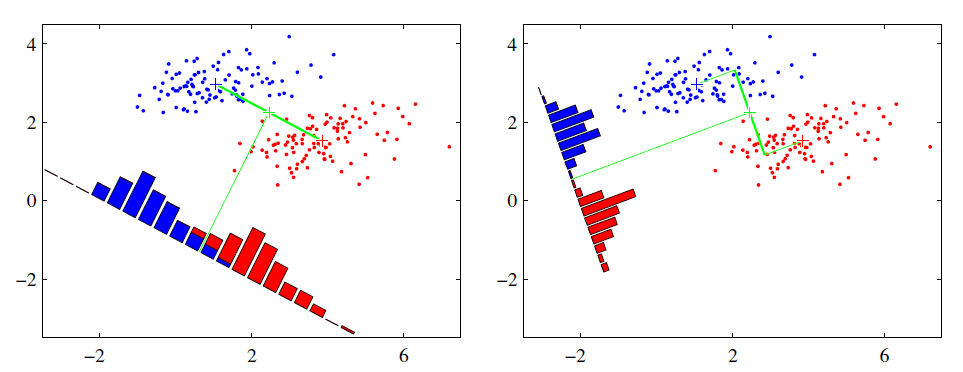
\includegraphics{./img/ch2/2.29/1.png}
\caption{}
\end{figure}

左图和右图是两种不同的投影方式。

​ 左图思路:让不同类别的平均点距离最远的投影方式。

​ 右图思路:让同类别的数据挨得最近的投影方式。

​
从上图直观看出,右图红色数据和蓝色数据在各自的区域来说相对集中,根据数据分布直方图也可看出,所以右图的投影效果好于左图,左图中间直方图部分有明显交集。

​
以上例子是基于数据是二维的,分类后的投影是一条直线。如果原始数据是多维的,则投影后的分类面是一低维的超平面。

\subsection{2.14.3
二类LDA算法原理}\label{ux4e8cux7c7bldaux7b97ux6cd5ux539fux7406}

​ 输入:数据集
$D={(\boldsymbol x_1,\boldsymbol y_1),(\boldsymbol x_2,\boldsymbol y_2),...,(\boldsymbol x_m,\boldsymbol y_m)}​$,其中样本
$\boldsymbol x_i ​$
是n维向量,$\boldsymbol y_i \epsilon {0, 1}​$,降维后的目标维度
$d​$。定义

​ $N_j(j=0,1)$ 为第 $j$ 类样本个数;

​ $X_j(j=0,1)$ 为第 $j$ 类样本的集合;

​ $u_j(j=0,1)​$ 为第 $j​$ 类样本的均值向量;

​ $\sum_j(j=0,1)$ 为第 $j$ 类样本的协方差矩阵。

​ 其中 \[
u_j = \frac{1}{N_j} \sum_{\boldsymbol x\epsilon X_j}\boldsymbol x(j=0,1), 
\sum_j = \sum_{\boldsymbol x\epsilon X_j}(\boldsymbol x-u_j)(\boldsymbol x-u_j)^T(j=0,1)
\] ​ 假设投影直线是向量 $\boldsymbol w$,对任意样本
$\boldsymbol x_i$,它在直线 $w$上的投影为
$\boldsymbol w^Tx_i$,两个类别的中心点 $u_0$, $u\_1 $在直线 $w$
的投影分别为 $\boldsymbol w^Tu_0$ 、$\boldsymbol w^Tu_1$。

​ LDA的目标是让两类别的数据中心间的距离
$\| \boldsymbol w^Tu_0 - \boldsymbol w^Tu_1 \|^2_2$
尽量大,与此同时,希望同类样本投影点的协方差$\boldsymbol w^T \sum_0 \boldsymbol w$、$\boldsymbol w^T \sum_1 \boldsymbol w$
尽量小,最小化
$\boldsymbol w^T \sum_0 \boldsymbol w + \boldsymbol w^T \sum_1 \boldsymbol w​$
。 ​ 定义 ​ 类内散度矩阵 \[
S_w = \sum_0 + \sum_1 = 
    \sum_{\boldsymbol x\epsilon X_0}(\boldsymbol x-u_0)(\boldsymbol x-u_0)^T + 
    \sum_{\boldsymbol x\epsilon X_1}(\boldsymbol x-u_1)(\boldsymbol x-u_1)^T
\] ​ 类间散度矩阵 $S_b = (u_0 - u_1)(u_0 - u_1)^T$

​ 据上分析,优化目标为
\[
\mathop{\arg\max}_\boldsymbol w J(\boldsymbol w) = \frac{\| \boldsymbol w^Tu_0 - \boldsymbol w^Tu_1 \|^2_2}{\boldsymbol w^T \sum_0\boldsymbol w + \boldsymbol w^T \sum_1\boldsymbol w} = 
\frac{\boldsymbol w^T(u_0-u_1)(u_0-u_1)^T\boldsymbol w}{\boldsymbol w^T(\sum_0 + \sum_1)\boldsymbol w} =
\frac{\boldsymbol w^TS_b\boldsymbol w}{\boldsymbol w^TS_w\boldsymbol w}
\] ​ 根据广义瑞利商的性质,矩阵 $S^{-1}_{w} S_b$ 的最大特征值为
$J(\boldsymbol w)$ 的最大值,矩阵 $S^{-1}_{w} S_b$
的最大特征值对应的特征向量即为 $\boldsymbol w$。

\subsection{LDA算法流程总结}\label{ldaux7b97ux6cd5ux6d41ux7a0bux603bux7ed3}

LDA算法降维流程如下:

​ 输入:数据集
$D = { (x_1,y_1),(x_2,y_2), ... ,(x_m,y_m) }$,其中样本 $x\_i $
是n维向量,$y_i \epsilon {C_1, C_2, ..., C_k}$,降维后的目标维度
$d$ 。

​ 输出:降维后的数据集 $\overline{D} $ 。

步骤: 1. 计算类内散度矩阵 $S_w$。 2. 计算类间散度矩阵 $S_b​$ 。 3.
计算矩阵 $S^{-1}_wS_b​$ 。 4. 计算矩阵 $S^{-1}_wS_b$ 的最大的 d
个特征值。 5. 计算 d 个特征值对应的 d 个特征向量,记投影矩阵为 W 。 6.
转化样本集的每个样本,得到新样本 $P_i = W^Tx_i​$ 。 7. 输出新样本集
$\overline{D} = { (p_1,y_1),(p_2,y_2),...,(p_m,y_m) }​$

\subsection{LDA和PCA区别}\label{ldaux548cpcaux533aux522b}

\begin{longtable}[]{ cll }
%\toprule
异同点 & LDA & PCA\tabularnewline
%\midrule
%\endhead
相同点 & 1. 两者均可以对数据进行降维;2.
两者在降维时均使用了矩阵特征分解的思想;3. 两者都假设数据符合高斯分布;
&\tabularnewline
不同点 & 有监督的降维方法; & 无监督的降维方法;\tabularnewline
& 降维最多降到k-1维; & 降维多少没有限制;\tabularnewline
& 可以用于降维,还可以用于分类; & 只用于降维;\tabularnewline
& 选择分类性能最好的投影方向; &
选择样本点投影具有最大方差的方向;\tabularnewline
& 更明确,更能反映样本间差异; & 目的较为模糊;\tabularnewline
% \bottomrule
\end{longtable}

\subsection{ LDA优缺点}\label{ldaux4f18ux7f3aux70b9}

\begin{longtable}[]{ cl }
%\toprule
\begin{minipage}[b]{0.05\columnwidth}\centering\strut
优缺点\strut
\end{minipage} & \begin{minipage}[b]{0.04\columnwidth}\raggedright\strut
简要说明\strut
\end{minipage}\tabularnewline
%\midrule
%\endhead
\begin{minipage}[t]{0.05\columnwidth}\centering\strut
优点\strut
\end{minipage} & \begin{minipage}[t]{0.04\columnwidth}\raggedright\strut
1. 可以使用类别的先验知识;2.
以标签、类别衡量差异性的有监督降维方式,相对于PCA的模糊性,其目的更明确,更能反映样本间的差异;\strut
\end{minipage}\tabularnewline
\begin{minipage}[t]{0.05\columnwidth}\centering\strut
缺点\strut
\end{minipage} & \begin{minipage}[t]{0.04\columnwidth}\raggedright\strut
1. LDA不适合对非高斯分布样本进行降维;2. LDA降维最多降到分类数k-1维;3.
LDA在样本分类信息依赖方差而不是均值时,降维效果不好;4.
LDA可能过度拟合数据。\strut
\end{minipage}\tabularnewline
% \bottomrule
\end{longtable}

\section{主成分分析(PCA)}\label{ux4e3bux6210ux5206ux5206ux6790pca}

\subsection{主成分分析(PCA)思想总结}\label{ux4e3bux6210ux5206ux5206ux6790pcaux601dux60f3ux603bux7ed3}

\begin{enumerate}
\def\labelenumi{\arabic{enumi}.}
% \tightlist
\item
  PCA就是将高维的数据通过线性变换投影到低维空间上去。
\item
  投影思想:找出最能够代表原始数据的投影方法。被PCA降掉的那些维度只能是那些噪声或是冗余的数据。
\item
  去冗余:去除可以被其他向量代表的线性相关向量,这部分信息量是多余的。
\item
  去噪声,去除较小特征值对应的特征向量,特征值的大小反映了变换后在特征向量方向上变换的幅度,幅度越大,说明这个方向上的元素差异也越大,要保留。
\item
  对角化矩阵,寻找极大线性无关组,保留较大的特征值,去除较小特征值,组成一个投影矩阵,对原始样本矩阵进行投影,得到降维后的新样本矩阵。
\item
  完成PCA的关键是------协方差矩阵。协方差矩阵,能同时表现不同维度间的相关性以及各个维度上的方差。协方差矩阵度量的是维度与维度之间的关系,而非样本与样本之间。
\item
  之所以对角化,因为对角化之后非对角上的元素都是0,达到去噪声的目的。对角化后的协方差矩阵,对角线上较小的新方差对应的就是那些该去掉的维度。所以我们只取那些含有较大能量(特征值)的维度,其余的就舍掉,即去冗余。
\end{enumerate}

\subsection{图解PCA核心思想}\label{ux56feux89e3pcaux6838ux5fc3ux601dux60f3}

​
PCA可解决训练数据中存在数据特征过多或特征累赘的问题。核心思想是将m维特征映射到n维(n
\textless{} m),这n维形成主元,是重构出来最能代表原始数据的正交特征。

​
假设数据集是m个n维,$(\boldsymbol x^{(1)}, \boldsymbol x^{(2)}, \cdots, \boldsymbol x^{(m)})$。如果$n=2$,需要降维到$n'=1$,现在想找到某一维度方向代表这两个维度的数据。下图有$u_1, u_2$两个向量方向,但是哪个向量才是我们所想要的,可以更好代表原始数据集的呢?

\begin{figure}
\centering
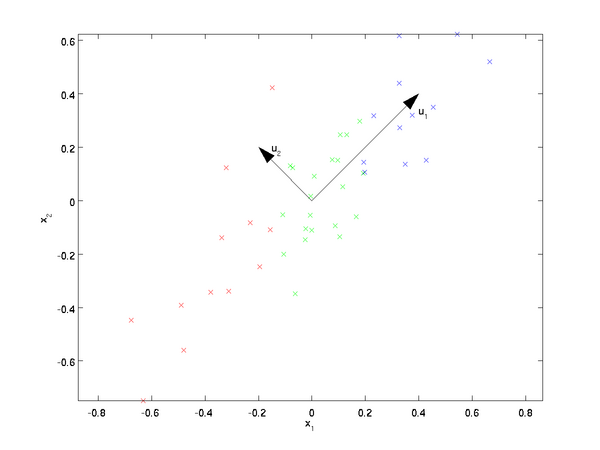
\includegraphics{./img/ch2/2.34/1.png}
\caption{}
\end{figure}

从图可看出,$u_1$比$u_2$好,为什么呢?有以下两个主要评价指标: 1.
样本点到这个直线的距离足够近。 2.
样本点在这个直线上的投影能尽可能的分开。

如果我们需要降维的目标维数是其他任意维,则: 1.
样本点到这个超平面的距离足够近。 2.
样本点在这个超平面上的投影能尽可能的分开。

\subsection{ PCA算法推理}\label{pcaux7b97ux6cd5ux63a8ux7406}

下面以基于最小投影距离为评价指标推理:

​
假设数据集是m个n维,$(x^{(1)}, x^{(2)},...,x^{(m)})$,且数据进行了中心化。经过投影变换得到新坐标为
${w_1,w_2,...,w_n}$,其中 $w$ 是标准正交基,即
$\| w \|_2 = 1$,$w^T_iw_j = 0$。

​ 经过降维后,新坐标为 ${ w_1,w_2,...,w_n }$,其中 $n'$
是降维后的目标维数。样本点 $x^{(i)}$ 在新坐标系下的投影为
$z^{(i)} = \left(z^{(i)}_1, z^{(i)}_2, ..., z^{(i)}_{n'} \right)$,其中
$z^{(i)}_j = w^T_j x^{(i)}$ 是 $x^{(i)} ​$ 在低维坐标系里第 j
维的坐标。

​ 如果用 $z^{(i)} $ 去恢复 $x^{(i)} $ ,则得到的恢复数据为
$\widehat{x}^{(i)} = \sum^{n'}_{j=1} x^{(i)}_j w_j = Wz^{(i)}$,其中
$W$为标准正交基组成的矩阵。

​ 考虑到整个样本集,样本点到这个超平面的距离足够近,目标变为最小化
$\sum^m_{i=1} \| \hat{x}^{(i)} - x^{(i)} \|^2_2$
。对此式进行推理,可得: \[
\sum^m_{i=1} \| \hat{x}^{(i)} - x^{(i)} \|^2_2 = 
    \sum^m_{i=1} \| Wz^{(i)} - x^{(i)} \|^2_2 \\
    = \sum^m_{i=1} \left( Wz^{(i)} \right)^T \left( Wz^{(i)} \right)
    - 2\sum^m_{i=1} \left( Wz^{(i)} \right)^T x^{(i)}
    + \sum^m_{i=1} \left( x^{(i)} \right)^T x^{(i)} \\
    = \sum^m_{i=1} \left( z^{(i)} \right)^T \left( z^{(i)} \right)
    - 2\sum^m_{i=1} \left( z^{(i)} \right)^T x^{(i)}
    + \sum^m_{i=1} \left( x^{(i)} \right)^T x^{(i)} \\
    = - \sum^m_{i=1} \left( z^{(i)} \right)^T \left( z^{(i)} \right)
    + \sum^m_{i=1} \left( x^{(i)} \right)^T x^{(i)} \\
    = -tr \left( W^T \left( \sum^m_{i=1} x^{(i)} \left( x^{(i)} \right)^T \right)W \right)
    + \sum^m_{i=1} \left( x^{(i)} \right)^T x^{(i)} \\
    = -tr \left( W^TXX^TW \right)
    + \sum^m_{i=1} \left( x^{(i)} \right)^T x^{(i)}
\]

​ 在推导过程中,分别用到了 $\overline{x}^{(i)} = Wz^{(i)}$
,矩阵转置公式
$(AB)^T = B^TA^T$,$W^TW = I$,$z^{(i)} = W^Tx^{(i)}$
以及矩阵的迹,最后两步是将代数和转为矩阵形式。 ​ 由于 $W$ 的每一个向量
$w_j$ 是标准正交基,$\sum^m_{i=1} x^{(i)} \left( x^{(i)} \right)^T$
是数据集的协方差矩阵,$\sum^m\_{i=1} \left( x^{(i)}
\right)^T x^{(i)} $ 是一个常量。最小化
$\sum^m_{i=1} \| \hat{x}^{(i)} - x^{(i)} \|^2_2$ 又可等价于 \[
\underbrace{\arg \min}_W - tr \left( W^TXX^TW \right) s.t.W^TW = I
\] 利用拉格朗日函数可得到 \[
J(W) = -tr(W^TXX^TW) + \lambda(W^TW - I)
\] ​ 对 $W$ 求导,可得 $-XX^TW + \lambda W = 0 $ ,也即 $
XX^TW = \lambda W $ 。 $ XX^T $ 是 $ n' $
个特征向量组成的矩阵,$\lambda$ 为$ XX^T $ 的特征值。$W$
即为我们想要的矩阵。 ​ 对于原始数据,只需要 $z^{(i)} = W^TX^{(i)}$
,就可把原始数据集降维到最小投影距离的 $n'$ 维数据集。

​ 基于最大投影方差的推导,这里就不再赘述,有兴趣的同仁可自行查阅资料。

\subsection{PCA算法流程总结}\label{pcaux7b97ux6cd5ux6d41ux7a0bux603bux7ed3}

输入:$n​$ 维样本集
$D = \left( x^{(1)},x^{(2)},...,x^{(m)} \right)​$ ,目标降维的维数
$n'​$ 。

输出:降维后的新样本集
$D' = \left( z^{(1)},z^{(2)},...,z^{(m)} \right)$ 。

主要步骤如下: 1. 对所有的样本进行中心化,$ x^{(i)} = x^{(i)}
- \frac{1}{m} \sum^m\_{j=1} x^{(j)} $ 。 2.
计算样本的协方差矩阵 $XX^T​$ 。 3. 对协方差矩阵 $XX^T$
进行特征值分解。 4. 取出最大的 $n' $ 个特征值对应的特征向量
${ w_1,w_2,...,w_{n'} }$ 。 5. 标准化特征向量,得到特征向量矩阵
$W$ 。 6. 转化样本集中的每个样本 $z^{(i)} = W^T x^{(i)}$ 。 7.
得到输出矩阵 $D' = \left( z^{(1)},z^{(2)},...,z^{(n)} \right)​$ 。
\emph{注}:在降维时,有时不明确目标维数,而是指定降维到的主成分比重阈值
$k(k \epsilon(0,1])​$ 。假设 $n​$ 个特征值为
$\lambda_1 \geqslant \lambda_2 \geqslant ... \geqslant \lambda_n​$
,则 $n'​$ 可从
$\sum^{n'}_{i=1} \lambda_i \geqslant k \times \sum^n_{i=1} \lambda_i ​$
得到。

\subsection{PCA算法主要优缺点}\label{pcaux7b97ux6cd5ux4e3bux8981ux4f18ux7f3aux70b9}

\begin{longtable}[]{ cl }
%\toprule
\begin{minipage}[b]{0.05\columnwidth}\centering\strut
优缺点\strut
\end{minipage} & \begin{minipage}[b]{0.04\columnwidth}\raggedright\strut
简要说明\strut
\end{minipage}\tabularnewline
%\midrule
%\endhead
\begin{minipage}[t]{0.05\columnwidth}\centering\strut
优点\strut
\end{minipage} & \begin{minipage}[t]{0.04\columnwidth}\raggedright\strut
1.
仅仅需要以方差衡量信息量,不受数据集以外的因素影响。 2.各主成分之间正交,可消除原始数据成分间的相互影响的因素。3.
计算方法简单,主要运算是特征值分解,易于实现。\strut
\end{minipage}\tabularnewline
\begin{minipage}[t]{0.05\columnwidth}\centering\strut
缺点\strut
\end{minipage} & \begin{minipage}[t]{0.04\columnwidth}\raggedright\strut
1.主成分各个特征维度的含义具有一定的模糊性,不如原始样本特征的解释性强。2.
方差小的非主成分也可能含有对样本差异的重要信息,因降维丢弃可能对后续数据处理有影响。\strut
\end{minipage}\tabularnewline
% \bottomrule
\end{longtable}

\subsection{降维的必要性及目的}\label{ux964dux7ef4ux7684ux5fc5ux8981ux6027ux53caux76eeux7684}

\textbf{降维的必要性}: 1.
多重共线性和预测变量之间相互关联。多重共线性会导致解空间的不稳定,从而可能导致结果的不连贯。
2.
高维空间本身具有稀疏性。一维正态分布有68\%的值落于正负标准差之间,而在十维空间上只有2\%。
3. 过多的变量,对查找规律造成冗余麻烦。 4.
仅在变量层面上分析可能会忽略变量之间的潜在联系。例如几个预测变量可能落入仅反映数据某一方面特征的一个组内。

\textbf{降维的目的}: 1. 减少预测变量的个数。 2.
确保这些变量是相互独立的。 3.
提供一个框架来解释结果。相关特征,特别是重要特征更能在数据中明确的显示出来;如果只有两维或者三维的话,更便于可视化展示。
4. 数据在低维下更容易处理、更容易使用。 5. 去除数据噪声。 6.
降低算法运算开销。

\subsection{KPCA与PCA的区别}\label{kpcaux4e0epcaux7684ux533aux522b}

​
应用PCA算法前提是假设存在一个线性超平面,进而投影。那如果数据不是线性的呢?该怎么办?这时候就需要KPCA,数据集从
$n$ 维映射到线性可分的高维 $N >n$,然后再从 $N$ 维降维到一个低维度
$n'(n'<n<N)$ 。

​
KPCA用到了核函数思想,使用了核函数的主成分分析一般称为核主成分分析(Kernelized
PCA, 简称KPCA)。

假设高维空间数据由 $n​$ 维空间的数据通过映射 $\phi​$ 产生。

​ $n$ 维空间的特征分解为: \[
\sum^m_{i=1} x^{(i)} \left( x^{(i)} \right)^T W = \lambda W
\]

​ 其映射为 \[
\sum^m_{i=1} \phi \left( x^{(i)} \right) \phi \left( x^{(i)} \right)^T W = \lambda W
\]

​
通过在高维空间进行协方差矩阵的特征值分解,然后用和PCA一样的方法进行降维。由于KPCA需要核函数的运算,因此它的计算量要比PCA大很多。

\section{ 模型评估}\label{ux6a21ux578bux8bc4ux4f30}

\subsection{模型评估常用方法?}\label{ux6a21ux578bux8bc4ux4f30ux5e38ux7528ux65b9ux6cd5}

​
一般情况来说,单一评分标准无法完全评估一个机器学习模型。只用good和bad偏离真实场景去评估某个模型,都是一种欠妥的评估方式。下面介绍常用的分类模型和回归模型评估方法。

\textbf{分类模型常用评估方法:}

\begin{longtable}[]{cc}
%\toprule
指标 & 描述\tabularnewline
%\midrule
%\endhead
Accuracy & 准确率\tabularnewline
Precision & 精准度/查准率\tabularnewline
Recall & 召回率/查全率\tabularnewline
P-R曲线 & 查准率为纵轴,查全率为横轴,作图\tabularnewline
F1 & F1值\tabularnewline
Confusion Matrix & 混淆矩阵\tabularnewline
ROC & ROC曲线\tabularnewline
AUC & ROC曲线下的面积\tabularnewline
% \bottomrule
\end{longtable}

\textbf{回归模型常用评估方法:}

\begin{longtable}[]{cc}
%\toprule
指标 & 描述\tabularnewline
%\midrule
%\endhead
Mean Square Error (MSE, RMSE) & 平均方差\tabularnewline
Absolute Error (MAE, RAE) & 绝对误差\tabularnewline
R-Squared & R平方值\tabularnewline
% \bottomrule
\end{longtable}

\subsection{2.16.2
误差、偏差和方差有什么区别和联系}\label{ux8befux5deeux504fux5deeux548cux65b9ux5deeux6709ux4ec0ux4e48ux533aux522bux548cux8054ux7cfb}

在机器学习中,Bias(偏差),Error(误差),和Variance(方差)存在以下区别和联系:

\textbf{对于Error }:

\begin{itemize}
\item
  误差(error):一般地,我们把学习器的实际预测输出与样本的真是输出之间的差异称为``误差''。
\item
  Error = Bias + Variance + Noise,Error反映的是整个模型的准确度。
\end{itemize}

\textbf{对于Noise:}

噪声:描述了在当前任务上任何学习算法所能达到的期望泛化误差的下界,即刻画了学习问题本身的难度。

\textbf{对于Bias:}

\begin{itemize}
% \tightlist
\item
  Bias衡量模型拟合训练数据的能力(训练数据不一定是整个 training
  dataset,而是只用于训练它的那一部分数据,例如:mini-batch),Bias反映的是模型在样本上的输出与真实值之间的误差,即模型本身的精准度。
\item
  Bias
  越小,拟合能力越高(可能产生overfitting);反之,拟合能力越低(可能产生underfitting)。
\item
  偏差越大,越偏离真实数据,如下图第二行所示。
\end{itemize}

\textbf{对于Variance:}

\begin{itemize}
\item
  方差公式:$S_{N}^{2}=\frac{1}{N}\sum_{i=1}^{N}(x_{i}-\bar{x})^{2}$
\item
  Variance描述的是预测值的变化范围,离散程度,也就是离其期望值的距离。方差越大,数据的分布越分散,模型的稳定程度越差。
\item
  Variance反映的是模型每一次输出结果与模型输出期望之间的误差,即模型的稳定性。
\item
  Variance越小,模型的泛化的能力越高;反之,模型的泛化的能力越低。
\item
  如果模型在训练集上拟合效果比较优秀,但是在测试集上拟合效果比较差劣,则方差较大,说明模型的稳定程度较差,出现这种现象可能是由于模型对训练集过拟合造成的。
  如下图右列所示。
\end{itemize}

% \begin{quote}
% \begin{figure}
% \centering
% 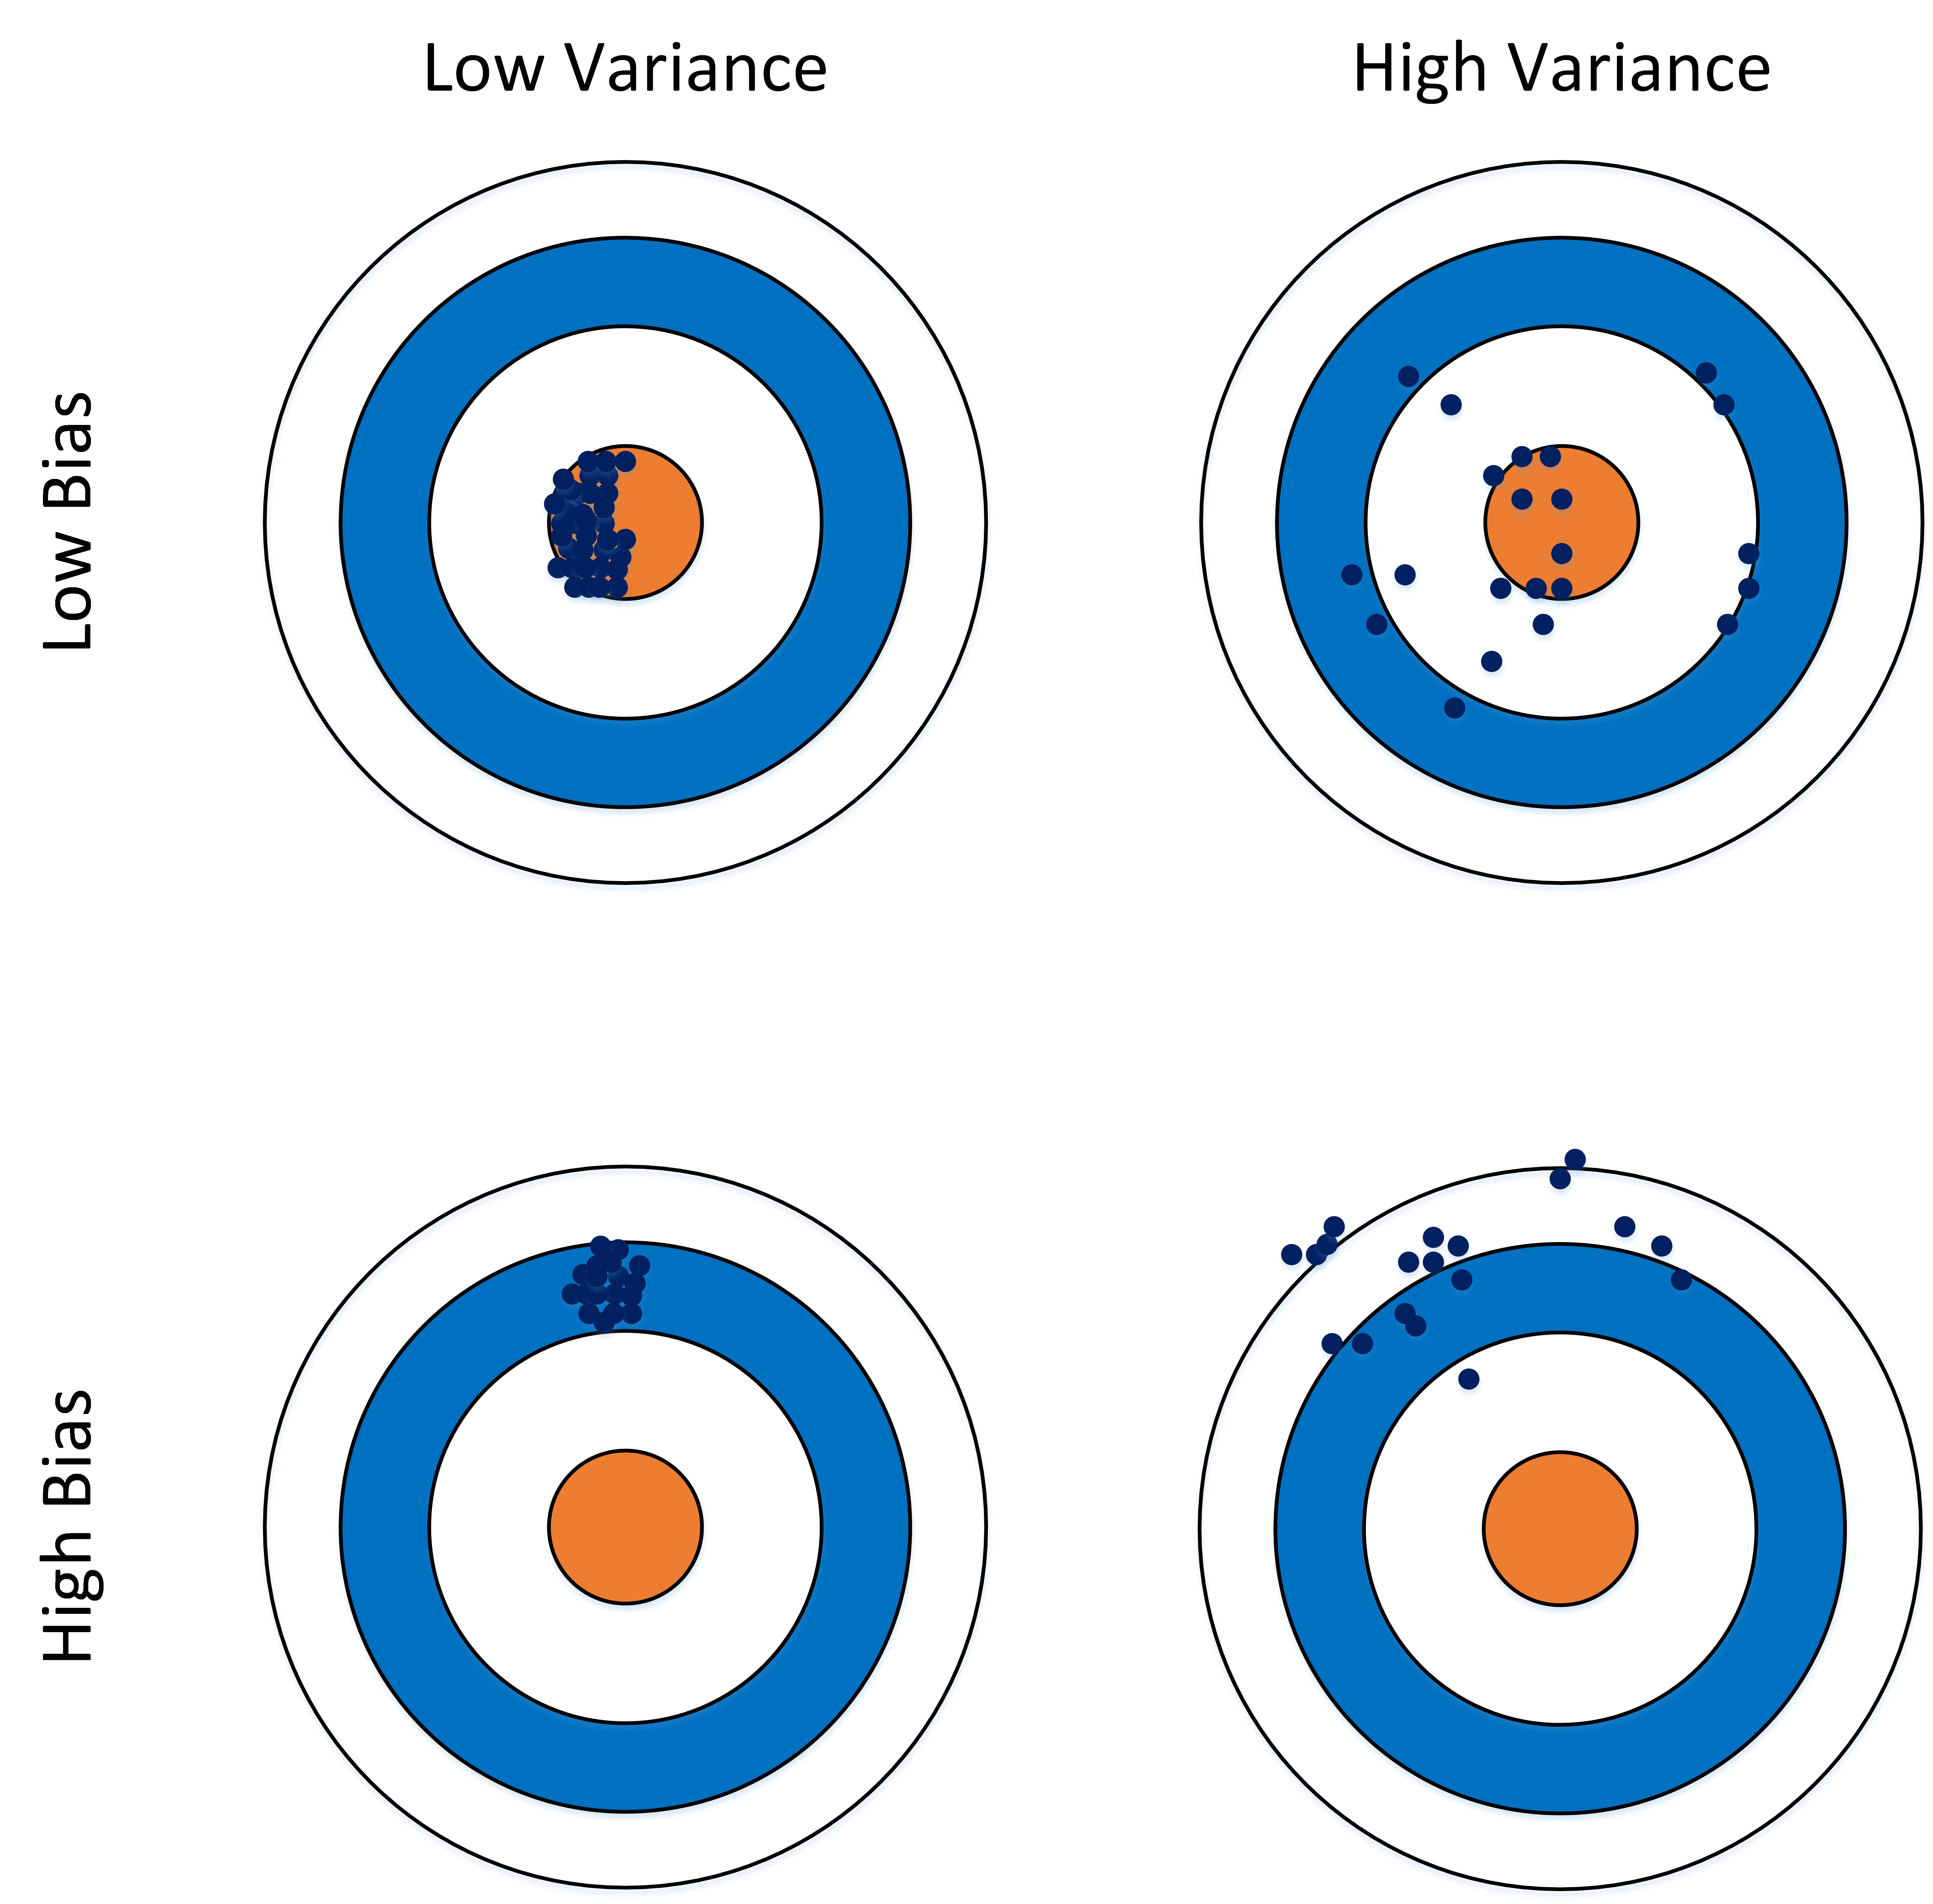
\includegraphics{./img/ch2/2.16.20.1.png}
% \caption{}
% \end{figure}
% \end{quote}

\subsection{经验误差与泛化误差}\label{ux7ecfux9a8cux8befux5deeux4e0eux6cdbux5316ux8befux5dee}

经验误差(empirical error):也叫训练误差(training
error),模型在训练集上的误差。

泛化误差(generalization
error):模型在新样本集(测试集)上的误差称为``泛化误差''。

\subsection{图解欠拟合、过拟合}\label{ux56feux89e3ux6b20ux62dfux5408ux8fc7ux62dfux5408}

根据不同的坐标方式,欠拟合与过拟合图解不同。 1.
\textbf{横轴为训练样本数量,纵轴为误差}

% \begin{figure}
% \centering
% 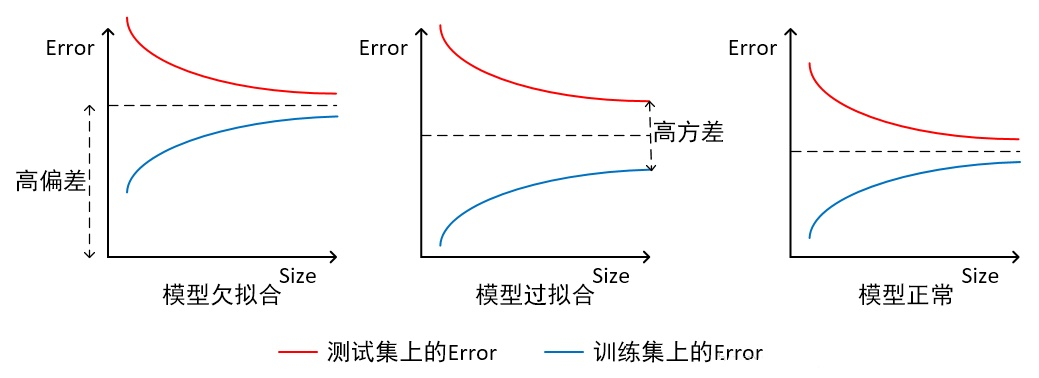
\includegraphics{./img/ch2/2.16.4.1.jpg}
% \caption{}
% \end{figure}

如上图所示,我们可以直观看出欠拟合和过拟合的区别:

​
模型欠拟合:在训练集以及测试集上同时具有较高的误差,此时模型的偏差较大;

​
模型过拟合:在训练集上具有较低的误差,在测试集上具有较高的误差,此时模型的方差较大。

​ 模型正常:在训练集以及测试集上,同时具有相对较低的偏差以及方差。

\begin{enumerate}
\def\labelenumi{\arabic{enumi}.}
\setcounter{enumi}{1}
% \tightlist
\item
  \textbf{横轴为模型复杂程度,纵轴为误差}
\end{enumerate}

% \begin{figure}
% \centering
% 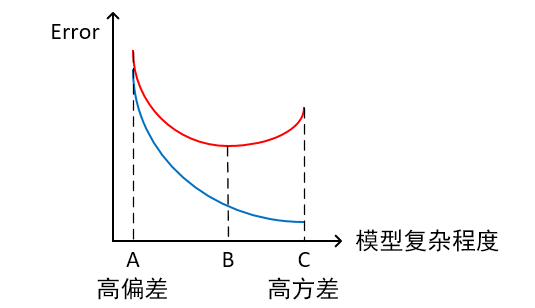
\includegraphics{./img/ch2/2.16.4.2.png}
% \caption{}
% \end{figure}

​ 红线为测试集上的Error,蓝线为训练集上的Error

​
模型欠拟合:模型在点A处,在训练集以及测试集上同时具有较高的误差,此时模型的偏差较大。

​
模型过拟合:模型在点C处,在训练集上具有较低的误差,在测试集上具有较高的误差,此时模型的方差较大。

​ 模型正常:模型复杂程度控制在点B处为最优。

\begin{enumerate}
\def\labelenumi{\arabic{enumi}.}
\setcounter{enumi}{2}
% \tightlist
\item
  \textbf{横轴为正则项系数,纵轴为误差}
\end{enumerate}

% \begin{figure}
% \centering
% 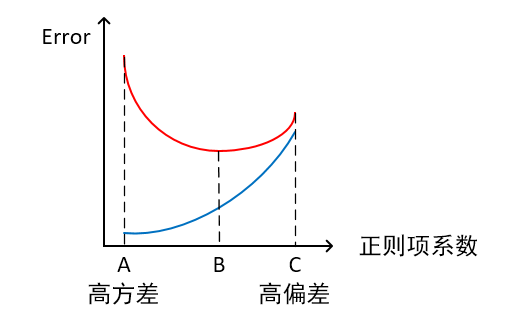
\includegraphics{./img/ch2/2.16.4.3.png}
% \caption{}
% \end{figure}

​ 红线为测试集上的Error,蓝线为训练集上的Error

​
模型欠拟合:模型在点C处,在训练集以及测试集上同时具有较高的误差,此时模型的偏差较大。

​
模型过拟合:模型在点A处,在训练集上具有较低的误差,在测试集上具有较高的误差,此时模型的方差较大。
它通常发生在模型过于复杂的情况下,如参数过多等,会使得模型的预测性能变弱,并且增加数据的波动性。虽然模型在训练时的效果可以表现的很完美,基本上记住了数据的全部特点,但这种模型在未知数据的表现能力会大减折扣,因为简单的模型泛化能力通常都是很弱的。

​ 模型正常:模型复杂程度控制在点B处为最优。

\subsection{如何解决过拟合与欠拟合}\label{ux5982ux4f55ux89e3ux51b3ux8fc7ux62dfux5408ux4e0eux6b20ux62dfux5408}

\textbf{如何解决欠拟合:} 1.
添加其他特征项。组合、泛化、相关性、上下文特征、平台特征等特征是特征添加的重要手段,有时候特征项不够会导致模型欠拟合。
2.
添加多项式特征。例如将线性模型添加二次项或三次项使模型泛化能力更强。例如,FM(Factorization
Machine)模型、FFM(Field-aware Factorization
Machine)模型,其实就是线性模型,增加了二阶多项式,保证了模型一定的拟合程度。
3. 可以增加模型的复杂程度。 4.
减小正则化系数。正则化的目的是用来防止过拟合的,但是现在模型出现了欠拟合,则需要减少正则化参数。

\textbf{如何解决过拟合:} 1.
重新清洗数据,数据不纯会导致过拟合,此类情况需要重新清洗数据。 2.
增加训练样本数量。 3. 降低模型复杂程度。 4. 增大正则项系数。 5.
采用dropout方法,dropout方法,通俗的讲就是在训练的时候让神经元以一定的概率不工作。
6. early stopping。 7. 减少迭代次数。 8. 增大学习率。 9. 添加噪声数据。
10. 树结构中,可以对树进行剪枝。 11. 减少特征项。

欠拟合和过拟合这些方法,需要根据实际问题,实际模型,进行选择。

\subsection{交叉验证的主要作用}\label{ux4ea4ux53c9ux9a8cux8bc1ux7684ux4e3bux8981ux4f5cux7528}

​
为了得到更为稳健可靠的模型,对模型的泛化误差进行评估,得到模型泛化误差的近似值。当有多个模型可以选择时,我们通常选择``泛化误差''最小的模型。

​ 交叉验证的方法有许多种,但是最常用的是:留一交叉验证、k折交叉验证。

\subsection{理解k折交叉验证}\label{ux7406ux89e3kux6298ux4ea4ux53c9ux9a8cux8bc1}

\begin{enumerate}
\def\labelenumi{\arabic{enumi}.}
% \tightlist
\item
  将含有N个样本的数据集,分成K份,每份含有N/K个样本。选择其中1份作为测试集,另外K-1份作为训练集,测试集就有K种情况。
\item
  在每种情况中,用训练集训练模型,用测试集测试模型,计算模型的泛化误差。
\item
  交叉验证重复K次,每份验证一次,平均K次的结果或者使用其它结合方式,最终得到一个单一估测,得到模型最终的泛化误差。
\item
  将K种情况下,模型的泛化误差取均值,得到模型最终的泛化误差。\\
\item
  一般$2\leqslant K \leqslant10$。
  k折交叉验证的优势在于,同时重复运用随机产生的子样本进行训练和验证,每次的结果验证一次,10折交叉验证是最常用的。
\item
  训练集中样本数量要足够多,一般至少大于总样本数的50\%。
\item
  训练集和测试集必须从完整的数据集中均匀取样。均匀取样的目的是希望减少训练集、测试集与原数据集之间的偏差。当样本数量足够多时,通过随机取样,便可以实现均匀取样的效果。
\end{enumerate}

\subsection{混淆矩阵}\label{ux6df7ux6dc6ux77e9ux9635}

第一种混淆矩阵:

\begin{longtable}[]{ cll }
%\toprule
真实情况T or F & 预测为正例1,P & 预测为负例0,N\tabularnewline
%\midrule
%\endhead
本来label标记为1,预测结果真为T、假为F & TP(预测为1,实际为1) &
FN(预测为0,实际为1)\tabularnewline
本来label标记为0,预测结果真为T、假为F & FP(预测为1,实际为0) &
TN(预测为0,实际也为0)\tabularnewline
% \bottomrule
\end{longtable}

第二种混淆矩阵:

\begin{longtable}[]{ cll }
%\toprule
预测情况P or N & 实际label为1,预测对了为T &
实际label为0,预测对了为T\tabularnewline
%\midrule
%\endhead
预测为正例1,P & TP(预测为1,实际为1) &
FP(预测为1,实际为0)\tabularnewline
预测为负例0,N & FN(预测为0,实际为1) &
TN(预测为0,实际也为0)\tabularnewline
% \bottomrule
\end{longtable}

\subsection{错误率及精度}\label{ux9519ux8befux7387ux53caux7cbeux5ea6}

\begin{enumerate}
\def\labelenumi{\arabic{enumi}.}
% \tightlist
\item
  错误率(Error Rate):分类错误的样本数占样本总数的比例。
\item
  精度(accuracy):分类正确的样本数占样本总数的比例。
\end{enumerate}

\subsection{查准率与查全率}\label{ux67e5ux51c6ux7387ux4e0eux67e5ux5168ux7387}

将算法预测的结果分成四种情况: 1. 正确肯定(True
Positive,TP):预测为真,实际为真 2. 正确否定(True
Negative,TN):预测为假,实际为假 3. 错误肯定(False
Positive,FP):预测为真,实际为假 4. 错误否定(False
Negative,FN):预测为假,实际为真

则:

查准率(Precision)=TP/(TP+FP)

\textbf{理解}:预测出为阳性的样本中,正确的有多少。区别准确率(正确预测出的样本,包括正确预测为阳性、阴性,占总样本比例)。
例,在所有我们预测有恶性肿瘤的病人中,实际上有恶性肿瘤的病人的百分比,越高越好。

查全率(Recall)=TP/(TP+FN)

\textbf{理解}:正确预测为阳性的数量占总样本中阳性数量的比例。
例,在所有实际上有恶性肿瘤的病人中,成功预测有恶性肿瘤的病人的百分比,越高越好。

\subsection{ROC与AUC}\label{rocux4e0eauc}

​ ROC全称是``受试者工作特征''(Receiver Operating Characteristic)。

​ ROC曲线的面积就是AUC(Area Under Curve)。

​ AUC用于衡量``二分类问题''机器学习算法性能(泛化能力)。

​
ROC曲线,通过将连续变量设定出多个不同的临界值,从而计算出一系列真正率和假正率,再以假正率为横坐标、真正率为纵坐标绘制成曲线,曲线下面积越大,推断准确性越高。在ROC曲线上,最靠近坐标图左上方的点为假正率和真正率均较高的临界值。

​
对于分类器,或者说分类算法,评价指标主要有Precision,Recall,F-score。下图是一个ROC曲线的示例。

% \begin{figure}
% \centering
% 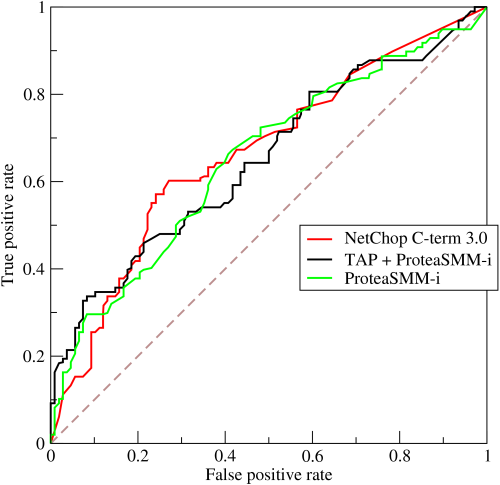
\includegraphics{./img/ch2/2.40.10/1.png}
% \caption{}
% \end{figure}

ROC曲线的横坐标为False Positive Rate(FPR),纵坐标为True Positive
Rate(TPR)。其中 \[
TPR = \frac{TP}{TP+FN} ,FPR = \frac{FP}{FP+TN}
\]

​ 下面着重介绍ROC曲线图中的四个点和一条线。 ​ 第一个点(0,1),即FPR=0,
TPR=1,这意味着FN(False Negative)=0,并且FP(False
Positive)=0。意味着这是一个完美的分类器,它将所有的样本都正确分类。 ​
第二个点(1,0),即FPR=1,TPR=0,意味着这是一个最糟糕的分类器,因为它成功避开了所有的正确答案。
​ 第三个点(0,0),即FPR=TPR=0,即FP(False Positive)=TP(True
Positive)=0,可以发现该分类器预测所有的样本都为负样本(Negative)。 ​
第四个点(1,1),即FPR=TPR=1,分类器实际上预测所有的样本都为正样本。 ​
经过以上分析,ROC曲线越接近左上角,该分类器的性能越好。

​ ROC曲线所覆盖的面积称为AUC(Area Under
Curve),可以更直观的判断学习器的性能,AUC越大则性能越好。

\subsection{如何画ROC曲线}\label{ux5982ux4f55ux753brocux66f2ux7ebf}

​
下图是一个示例,图中共有20个测试样本,``Class''一栏表示每个测试样本真正的标签(p表示正样本,n表示负样本),``Score''表示每个测试样本属于正样本的概率。

步骤: 1、假设已经得出一系列样本被划分为正类的概率,按照大小排序。
2、从高到低,依次将``Score''值作为阈值threshold,当测试样本属于正样本的概率大于或等于这个threshold时,我们认为它为正样本,否则为负样本。举例来说,对于图中的第4个样本,其``Score''值为0.6,那么样本1,2,3,4都被认为是正样本,因为它们的``Score''值都大于等于0.6,而其他样本则都认为是负样本。
3、每次选取一个不同的threshold,得到一组FPR和TPR,即ROC曲线上的一点。以此共得到20组FPR和TPR的值。
4、根据3、中的每个坐标点,画图。

% \begin{figure}
% \centering
% 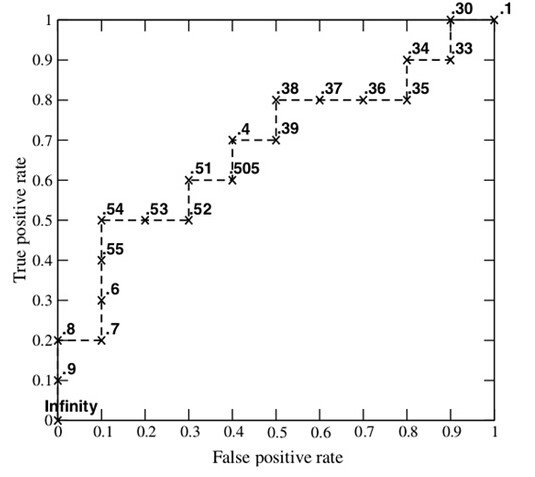
\includegraphics{./img/ch2/2.40.11/1.jpg}
% \caption{}
% \end{figure}

\subsection{如何计算TPR,FPR}\label{ux5982ux4f55ux8ba1ux7b97tprfpr}

1、分析数据 y\_true = {[}0, 0, 1, 1{]};scores = {[}0.1, 0.4, 0.35,
0.8{]}; 2、列表

\begin{longtable}[]{ lll }
%\toprule
样本 & 预测属于P的概率(score) & 真实类别\tabularnewline
%\midrule
%\endhead
y{[}0{]} & 0.1 & N\tabularnewline
y{[}1{]} & 0.4 & N\tabularnewline
y{[}2{]} & 0.35 & P\tabularnewline
y{[}3{]} & 0.8 & P\tabularnewline
% \bottomrule
\end{longtable}

3、将截断点依次取为score值,计算TPR和FPR。 当截断点为0.1时:
说明只要score\textgreater{}=0.1,它的预测类别就是正例。
因为4个样本的score都大于等于0.1,所以,所有样本的预测类别都为P。 scores
= {[}0.1, 0.4, 0.35, 0.8{]};y\_true = {[}0, 0, 1, 1{]};y\_pred = {[}1,
1, 1, 1{]}; 正例与反例信息如下:

\begin{longtable}[]{ lll }
%\toprule
& 正例 & 反例\tabularnewline
%\midrule
%\endhead
\textbf{正例} & TP=2 & FN=0\tabularnewline
\textbf{反例} & FP=2 & TN=0\tabularnewline
% \bottomrule
\end{longtable}

由此可得: TPR = TP/(TP+FN) = 1; FPR = FP/(TN+FP) = 1;

当截断点为0.35时: scores = {[}0.1, 0.4, 0.35, 0.8{]};y\_true = {[}0,
0, 1, 1{]};y\_pred = {[}0, 1, 1, 1{]}; 正例与反例信息如下:

\begin{longtable}[]{ lll }
%\toprule
& 正例 & 反例\tabularnewline
%\midrule
%\endhead
\textbf{正例} & TP=2 & FN=0\tabularnewline
\textbf{反例} & FP=1 & TN=1\tabularnewline
% \bottomrule
\end{longtable}

由此可得: TPR = TP/(TP+FN) = 1; FPR = FP/(TN+FP) = 0.5;

当截断点为0.4时: scores = {[}0.1, 0.4, 0.35, 0.8{]};y\_true = {[}0, 0,
1, 1{]};y\_pred = {[}0, 1, 0, 1{]}; 正例与反例信息如下:

\begin{longtable}[]{ lll }
%\toprule
& 正例 & 反例\tabularnewline
%\midrule
%\endhead
\textbf{正例} & TP=1 & FN=1\tabularnewline
\textbf{反例} & FP=1 & TN=1\tabularnewline
% \bottomrule
\end{longtable}

由此可得: TPR = TP/(TP+FN) = 0.5; FPR = FP/(TN+FP) = 0.5;

当截断点为0.8时: scores = {[}0.1, 0.4, 0.35, 0.8{]};y\_true = {[}0, 0,
1, 1{]};y\_pred = {[}0, 0, 0, 1{]};

正例与反例信息如下:

\begin{longtable}[]{ lll }
%\toprule
& 正例 & 反例\tabularnewline
%\midrule
%\endhead
\textbf{正例} & TP=1 & FN=1\tabularnewline
\textbf{反例} & FP=0 & TN=2\tabularnewline
% \bottomrule
\end{longtable}

由此可得: TPR = TP/(TP+FN) = 0.5; FPR = FP/(TN+FP) = 0;

4、根据TPR、FPR值,以FPR为横轴,TPR为纵轴画图。

\subsection{如何计算AUC}\label{ux5982ux4f55ux8ba1ux7b97auc}

\begin{itemize}
% \tightlist
\item
  将坐标点按照横坐标FPR排序 。
\item
  计算第$i$个坐标点和第$i+1$个坐标点的间距$dx$ 。
\item
  获取第$i$或者$i+1$个坐标点的纵坐标y。
\item
  计算面积微元$ds=ydx$。
\item
  对面积微元进行累加,得到AUC。
\end{itemize}

\subsection{为什么使用Roc和Auc评价分类器}\label{ux4e3aux4ec0ux4e48ux4f7fux7528rocux548caucux8bc4ux4ef7ux5206ux7c7bux5668}

​ 模型有很多评估方法,为什么还要使用ROC和AUC呢? ​
因为ROC曲线有个很好的特性:当测试集中的正负样本的分布变换的时候,ROC曲线能够保持不变。在实际的数据集中经常会出现样本类不平衡,即正负样本比例差距较大,而且测试数据中的正负样本也可能随着时间变化。

\subsection{直观理解AUC}\label{ux76f4ux89c2ux7406ux89e3auc}

​ 下图展现了三种AUC的值:

% \begin{figure}
% \centering
% 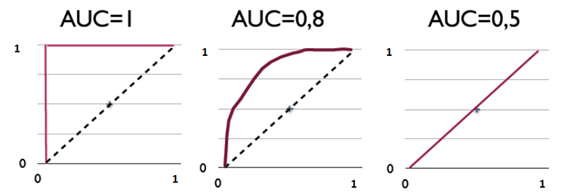
\includegraphics{./img/ch2/2.40.15/1.png}
% \caption{}
% \end{figure}

​
AUC是衡量二分类模型优劣的一种评价指标,表示正例排在负例前面的概率。其他评价指标有精确度、准确率、召回率,而AUC比这三者更为常用。
​
一般在分类模型中,预测结果都是以概率的形式表现,如果要计算准确率,通常都会手动设置一个阈值来将对应的概率转化成类别,这个阈值也就很大程度上影响了模型准确率的计算。
​ 举例: ​
现在假设有一个训练好的二分类器对10个正负样本(正例5个,负例5个)预测,得分按高到低排序得到的最好预测结果为{[}1,
1, 1, 1, 1, 0, 0, 0, 0,
0{]},即5个正例均排在5个负例前面,正例排在负例前面的概率为100\%。然后绘制其ROC曲线,由于是10个样本,除去原点我们需要描10个点,如下:

% \begin{figure}
% \centering
% 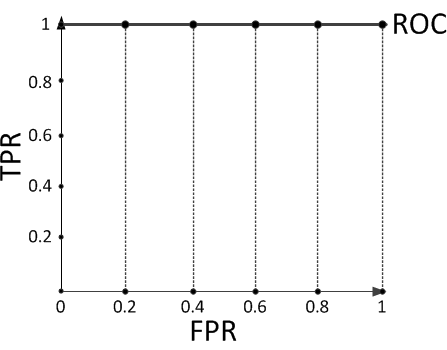
\includegraphics{./img/ch2/2.16.17-1.png}
% \caption{}
% \end{figure}

​
描点方式按照样本预测结果的得分高低从左至右开始遍历。从原点开始,每遇到1便向y轴正方向移动y轴最小步长1个单位,这里是1/5=0.2;每遇到0则向x轴正方向移动x轴最小步长1个单位,这里也是0.2。不难看出,上图的AUC等于1,印证了正例排在负例前面的概率的确为100\%。

​ 假设预测结果序列为{[}1, 1, 1, 1, 0, 1, 0, 0, 0, 0{]}。

% \begin{figure}
% \centering
% 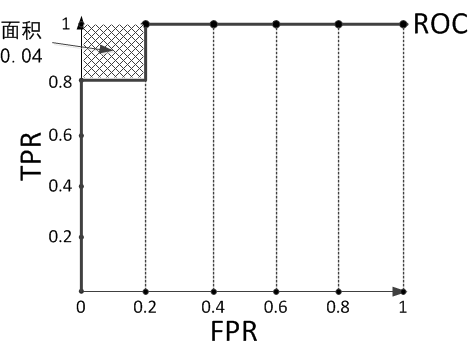
\includegraphics{./img/ch2/2.16.17-2.png}
% \caption{}
% \end{figure}

​ 计算上图的AUC为0.96与计算正例与排在负例前面的概率0.8 × 1 + 0.2 × 0.8 =
0.96相等,而左上角阴影部分的面积则是负例排在正例前面的概率0.2 × 0.2 =
0.04。

​ 假设预测结果序列为{[}1, 1, 1, 0, 1, 0, 1, 0, 0, 0{]}。

% \begin{figure}
% \centering
% 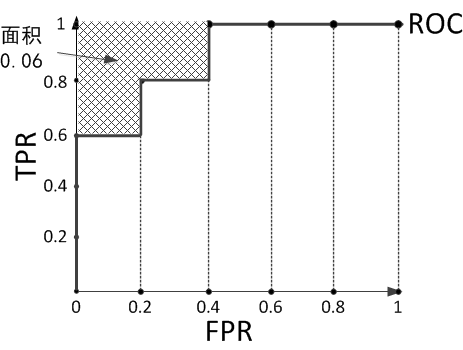
\includegraphics{./img/ch2/2.16.17-3.png}
 
% \end{figure}

​ 计算上图的AUC为0.88与计算正例与排在负例前面的概率0.6 × 1 + 0.2 × 0.8 +
0.2 × 0.6 = 0.88相等,左上角阴影部分的面积是负例排在正例前面的概率0.2 ×
0.2 × 3 = 0.12。

\subsection{代价敏感错误率与代价曲线}\label{ux4ee3ux4ef7ux654fux611fux9519ux8befux7387ux4e0eux4ee3ux4ef7ux66f2ux7ebf}

不同的错误会产生不同代价。以二分法为例,设置代价矩阵如下:

% \begin{figure}
% \centering
% 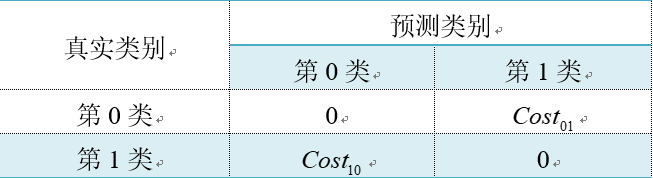
\includegraphics{./img/ch2/2-1.png}
 
% \end{figure}

当判断正确的时候,值为0,不正确的时候,分别为$Cost_{01}​$和$Cost_{10}​$
。

$Cost_{10}$:表示实际为反例但预测成正例的代价。

$Cost_{01}$:表示实际为正例但是预测为反例的代价。

\textbf{代价敏感错误率}=样本中由模型得到的错误值与代价乘积之和 /
总样本。 其数学表达式为: \[
E(f;D;cost)=\frac{1}{m}\left( \sum_{x_{i} \in D^{+}}({f(x_i)\neq y_i})\times Cost_{01}+ \sum_{x_{i} \in D^{-}}({f(x_i)\neq y_i})\times Cost_{10}\right)
\]
$D^{+}、D^{-}​$分别代表样例集的正例子集和反例子集,x是预测值,y是真实值。

\textbf{代价曲线}:
在均等代价时,ROC曲线不能直接反应出模型的期望总体代价,而代价曲线可以。
代价曲线横轴为{[}0,1{]}的正例函数代价: \[
P(+)Cost=\frac{p*Cost_{01}}{p*Cost_{01}+(1-p)*Cost_{10}}
\] 其中p是样本为正例的概率。

代价曲线纵轴维{[}0,1{]}的归一化代价: \[
Cost_{norm}=\frac{FNR*p*Cost_{01}+FNR*(1-p)*Cost_{10}}{p*Cost_{01}+(1-p)*Cost_{10}}
\]

其中FPR为假阳率,FNR=1-TPR为假阴率。

注:ROC每个点,对应代价平面上一条线。

例如,ROC上(TPR,FPR),计算出FNR=1-TPR,在代价平面上绘制一条从(0,FPR)到(1,FNR)的线段,面积则为该条件下期望的总体代价。所有线段下界面积,所有条件下学习器的期望总体代价。

% \begin{figure}
% \centering
% 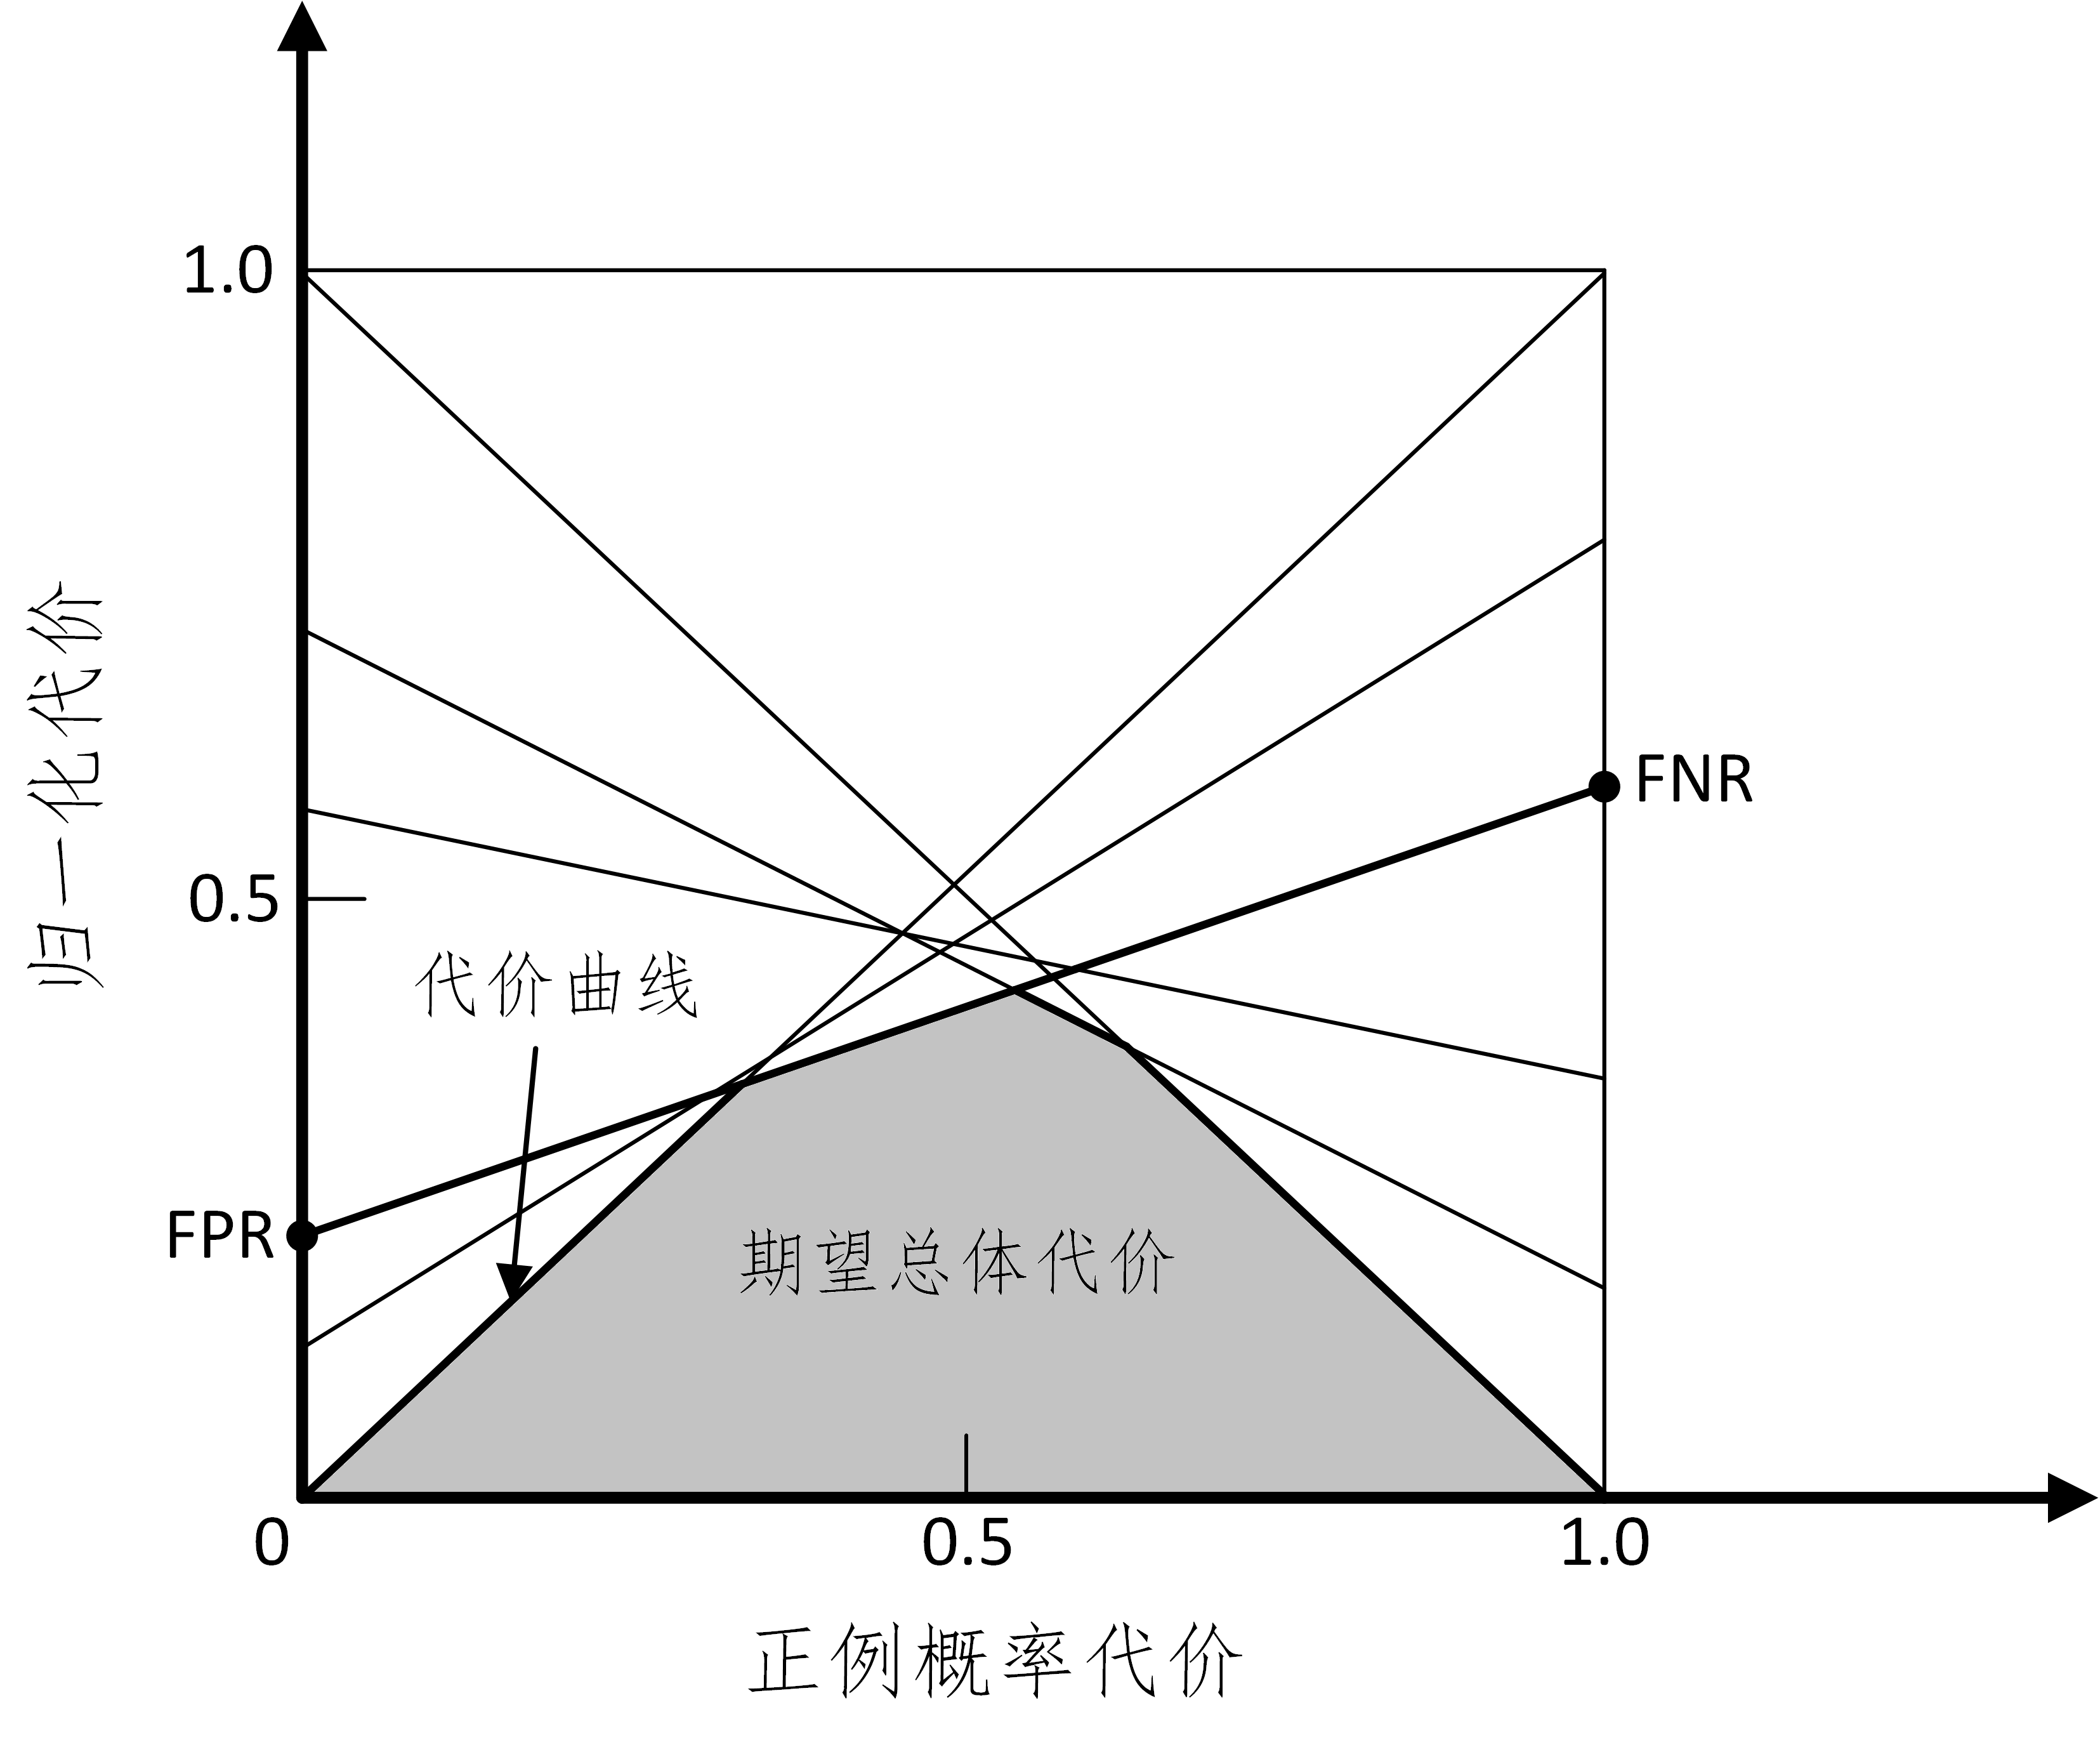
\includegraphics{./img/ch2/2.16.18.1.png}
 
% \end{figure}

\subsection{模型有哪些比较检验方法}\label{ux6a21ux578bux6709ux54eaux4e9bux6bd4ux8f83ux68c0ux9a8cux65b9ux6cd5}

正确性分析:模型稳定性分析,稳健性分析,收敛性分析,变化趋势分析,极值分析等。
有效性分析:误差分析,参数敏感性分析,模型对比检验等。
有用性分析:关键数据求解,极值点,拐点,变化趋势分析,用数据验证动态模拟等。
高效性分析:时空复杂度分析与现有进行比较等。

\subsection{为什么使用标准差}\label{ux4e3aux4ec0ux4e48ux4f7fux7528ux6807ux51c6ux5dee}

方差公式为:$S^2_{N}=\frac{1}{N}\sum_{i=1}^{N}(x_{i}-\bar{x})^{2}​$

标准差公式为:$S_{N}=\sqrt{\frac{1}{N}\sum_{i=1}^{N}(x_{i}-\bar{x})^{2}}​$

样本标准差公式为:$S_{N}=\sqrt{\frac{1}{N-1}\sum_{i=1}^{N}(x_{i}-\bar{x})^{2}}​$

与方差相比,使用标准差来表示数据点的离散程度有3个好处:
1、表示离散程度的数字与样本数据点的数量级一致,更适合对数据样本形成感性认知。

2、表示离散程度的数字单位与样本数据的单位一致,更方便做后续的分析运算。

3、在样本数据大致符合正态分布的情况下,标准差具有方便估算的特性:68\%的数据点落在平均值前后1个标准差的范围内、95\%的数据点落在平均值前后2个标准差的范围内,而99\%的数据点将会落在平均值前后3个标准差的范围内。

\subsection{类别不平衡产生原因}\label{ux7c7bux522bux4e0dux5e73ux8861ux4ea7ux751fux539fux56e0}

​
类别不平衡(class-imbalance)是指分类任务中不同类别的训练样例数目差别很大的情况。

产生原因:

​
分类学习算法通常都会假设不同类别的训练样例数目基本相同。如果不同类别的训练样例数目差别很大,则会影响学习结果,测试结果变差。例如二分类问题中有998个反例,正例有2个,那学习方法只需返回一个永远将新样本预测为反例的分类器,就能达到99.8\%的精度;然而这样的分类器没有价值。
\#\#\# 2.16.21 常见的类别不平衡问题解决方法
  防止类别不平衡对学习造成的影响,在构建分类模型之前,需要对分类不平衡性问题进行处理。主要解决方法有:

1、扩大数据集

​ 增加包含小类样本数据的数据,更多的数据能得到更多的分布信息。

2、对大类数据欠采样

​ 减少大类数据样本个数,使与小样本个数接近。 ​
缺点:欠采样操作时若随机丢弃大类样本,可能会丢失重要信息。 ​
代表算法:EasyEnsemble。其思想是利用集成学习机制,将大类划分为若干个集合供不同的学习器使用。相当于对每个学习器都进行欠采样,但对于全局则不会丢失重要信息。

3、对小类数据过采样

​ 过采样:对小类的数据样本进行采样来增加小类的数据样本个数。

​ 代表算法:SMOTE和ADASYN。

​ SMOTE:通过对训练集中的小类数据进行插值来产生额外的小类样本数据。

​
新的少数类样本产生的策略:对每个少数类样本a,在a的最近邻中随机选一个样本b,然后在a、b之间的连线上随机选一点作为新合成的少数类样本。\\
​
ADASYN:根据学习难度的不同,对不同的少数类别的样本使用加权分布,对于难以学习的少数类的样本,产生更多的综合数据。
通过减少类不平衡引入的偏差和将分类决策边界自适应地转移到困难的样本两种手段,改善了数据分布。

4、使用新评价指标

​
如果当前评价指标不适用,则应寻找其他具有说服力的评价指标。比如准确度这个评价指标在类别不均衡的分类任务中并不适用,甚至进行误导。因此在类别不均衡分类任务中,需要使用更有说服力的评价指标来对分类器进行评价。

5、选择新算法

​ 不同的算法适用于不同的任务与数据,应该使用不同的算法进行比较。

6、数据代价加权

​
例如当分类任务是识别小类,那么可以对分类器的小类样本数据增加权值,降低大类样本的权值,从而使得分类器将重点集中在小类样本身上。

7、转化问题思考角度

​
例如在分类问题时,把小类的样本作为异常点,将问题转化为异常点检测或变化趋势检测问题。
异常点检测即是对那些罕见事件进行识别。变化趋势检测区别于异常点检测在于其通过检测不寻常的变化趋势来识别。

8、将问题细化分析

​
对问题进行分析与挖掘,将问题划分成多个更小的问题,看这些小问题是否更容易解决。

\section{决策树}\label{ux51b3ux7b56ux6811}

\subsection{决策树的基本原理}\label{ux51b3ux7b56ux6811ux7684ux57faux672cux539fux7406}

​ 决策树(Decision
Tree)是一种分而治之的决策过程。一个困难的预测问题,通过树的分支节点,被划分成两个或多个较为简单的子集,从结构上划分为不同的子问题。将依规则分割数据集的过程不断递归下去(Recursive
Partitioning)。随着树的深度不断增加,分支节点的子集越来越小,所需要提的问题数也逐渐简化。当分支节点的深度或者问题的简单程度满足一定的停止规则(Stopping
Rule)时, 该分支节点会停止分裂,此为自上而下的停止阈值(Cutoff
Threshold)法;有些决策树也使用自下而上的剪枝(Pruning)法。

\subsection{决策树的三要素?}\label{ux51b3ux7b56ux6811ux7684ux4e09ux8981ux7d20}

​ 一棵决策树的生成过程主要分为下3个部分:

​
1、特征选择:从训练数据中众多的特征中选择一个特征作为当前节点的分裂标准,如何选择特征有着很多不同量化评估标准,从而衍生出不同的决策树算法。

​
2、决策树生成:根据选择的特征评估标准,从上至下递归地生成子节点,直到数据集不可分则决策树停止生长。树结构来说,递归结构是最容易理解的方式。

​
3、剪枝:决策树容易过拟合,一般来需要剪枝,缩小树结构规模、缓解过拟合。剪枝技术有预剪枝和后剪枝两种。

\subsection{决策树学习基本算法}\label{ux51b3ux7b56ux6811ux5b66ux4e60ux57faux672cux7b97ux6cd5}

% \begin{figure}
% \centering
% 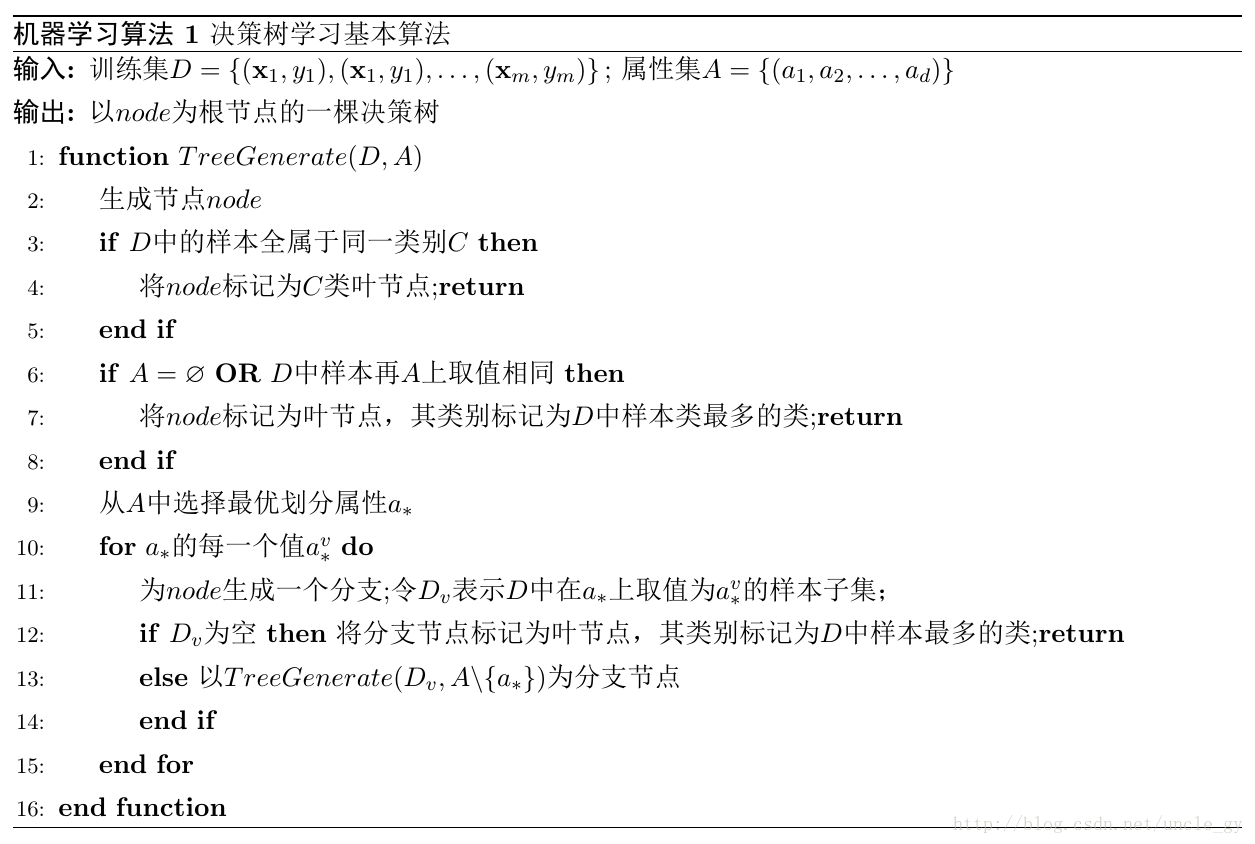
\includegraphics{./img/ch2/2-5.png}
 
% \end{figure}

\subsection{决策树算法优缺点}\label{ux51b3ux7b56ux6811ux7b97ux6cd5ux4f18ux7f3aux70b9}

\textbf{决策树算法的优点}:

1、决策树算法易理解,机理解释起来简单。

2、决策树算法可以用于小数据集。

3、决策树算法的时间复杂度较小,为用于训练决策树的数据点的对数。

4、相比于其他算法智能分析一种类型变量,决策树算法可处理数字和数据的类别。

5、能够处理多输出的问题。

6、对缺失值不敏感。

7、可以处理不相关特征数据。

8、效率高,决策树只需要一次构建,反复使用,每一次预测的最大计算次数不超过决策树的深度。

\textbf{决策树算法的缺点}:

1、对连续性的字段比较难预测。

2、容易出现过拟合。

3、当类别太多时,错误可能就会增加的比较快。

4、在处理特征关联性比较强的数据时表现得不是太好。

5、对于各类别样本数量不一致的数据,在决策树当中,信息增益的结果偏向于那些具有更多数值的特征。

\subsection{熵的概念以及理解}\label{ux71b5ux7684ux6982ux5ff5ux4ee5ux53caux7406ux89e3}

​ 熵:度量随机变量的不确定性。\\
​
定义:假设随机变量X的可能取值有$x_{1},x_{2},...,x_{n}$,对于每一个可能的取值$x_{i}$,其概率为$P(X=x_{i})=p_{i},i=1,2...,n$。随机变量的熵为:
\[
H(X)=-\sum_{i=1}^{n}p_{i}log_{2}p_{i}
\] ​
对于样本集合,假设样本有k个类别,每个类别的概率为$\frac{|C_{k}|}{|D|}$,其中
${|C_{k}|}{|D|}$为类别为k的样本个数,$|D|​$为样本总数。样本集合D的熵为:
\[
H(D)=-\sum_{k=1}^{k}\frac{|C_{k}|}{|D|}log_{2}\frac{|C_{k}|}{|D|}
\]

\subsection{信息增益的理解}\label{ux4fe1ux606fux589eux76caux7684ux7406ux89e3}

​ 定义:以某特征划分数据集前后的熵的差值。 ​
熵可以表示样本集合的不确定性,熵越大,样本的不确定性就越大。因此可以使用划分前后集合熵的差值来衡量使用当前特征对于样本集合D划分效果的好坏。
​
假设划分前样本集合D的熵为H(D)。使用某个特征A划分数据集D,计算划分后的数据子集的熵为H(D\textbar{}A)。\\
​ 则信息增益为: \[
g(D,A)=H(D)-H(D|A)
\] ​
\emph{注:}在决策树构建的过程中我们总是希望集合往最快到达纯度更高的子集合方向发展,因此我们总是选择使得信息增益最大的特征来划分当前数据集D。\\
​
思想:计算所有特征划分数据集D,得到多个特征划分数据集D的信息增益,从这些信息增益中选择最大的,因而当前结点的划分特征便是使信息增益最大的划分所使用的特征。\\
​ 另外这里提一下信息增益比相关知识: ​
$信息增益比=惩罚参数\times信息增益$\\
​
信息增益比本质:在信息增益的基础之上乘上一个惩罚参数。特征个数较多时,惩罚参数较小;特征个数较少时,惩罚参数较大。\\
​ 惩罚参数:数据集D以特征A作为随机变量的熵的倒数。

\subsection{剪枝处理的作用及策略}\label{ux526aux679dux5904ux7406ux7684ux4f5cux7528ux53caux7b56ux7565}

​ 剪枝处理是决策树学习算法用来解决过拟合问题的一种办法。

​ 在决策树算法中,为了尽可能正确分类训练样本, 节点划分过程不断重复,
有时候会造成决策树分支过多,以至于将训练样本集自身特点当作泛化特点,
而导致过拟合。 因此可以采用剪枝处理来去掉一些分支来降低过拟合的风险。

​ 剪枝的基本策略有预剪枝(pre-pruning)和后剪枝(post-pruning)。

​ 预剪枝:在决策树生成过程中,在每个节点划分前先估计其划分后的泛化性能,
如果不能提升,则停止划分,将当前节点标记为叶结点。

​ 后剪枝:生成决策树以后,再自下而上对非叶结点进行考察,
若将此节点标记为叶结点可以带来泛化性能提升,则修改之。

\section{ 支持向量机}\label{ux652fux6301ux5411ux91cfux673a}

\subsection{什么是支持向量机}\label{ux4ec0ux4e48ux662fux652fux6301ux5411ux91cfux673a}

​
支持向量:在求解的过程中,会发现只根据部分数据就可以确定分类器,这些数据称为支持向量。

​ 支持向量机(Support Vector
Machine,SVM):其含义是通过支持向量运算的分类器。

​
在一个二维环境中,其中点R,S,G点和其它靠近中间黑线的点可以看作为支持向量,它们可以决定分类器,即黑线的具体参数。

% \begin{figure}
% \centering
% 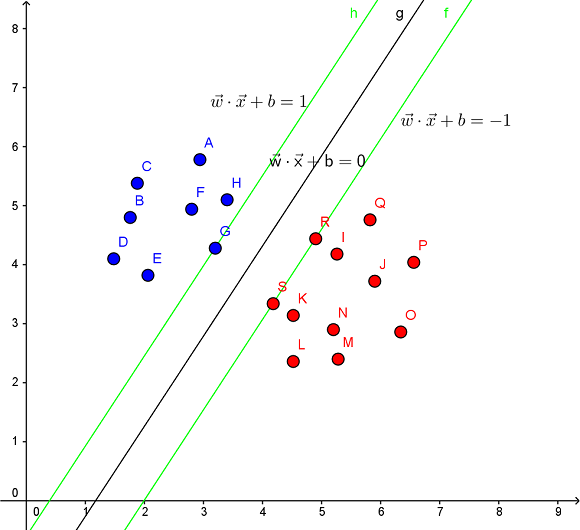
\includegraphics{./img/ch2/2-6.png}
 
% \end{figure}

​
支持向量机是一种二分类模型,它的目的是寻找一个超平面来对样本进行分割,分割的原则是边界最大化,最终转化为一个凸二次规划问题来求解。由简至繁的模型包括:

​ 当训练样本线性可分时,通过硬边界(hard
margin)最大化,学习一个线性可分支持向量机;

​ 当训练样本近似线性可分时,通过软边界(soft
margin)最大化,学习一个线性支持向量机;

​
当训练样本线性不可分时,通过核技巧和软边界最大化,学习一个非线性支持向量机;

\subsection{支持向量机能解决哪些问题}\label{ux652fux6301ux5411ux91cfux673aux80fdux89e3ux51b3ux54eaux4e9bux95eeux9898}

\textbf{线性分类}

​
在训练数据中,每个数据都有n个的属性和一个二分类类别标志,我们可以认为这些数据在一个n维空间里。我们的目标是找到一个n-1维的超平面,这个超平面可以将数据分成两部分,每部分数据都属于同一个类别。

​
这样的超平面有很多,假如我们要找到一个最佳的超平面。此时,增加一个约束条件:要求这个超平面到每边最近数据点的距离是最大的,成为最大边距超平面。这个分类器即为最大边距分类器。

\textbf{非线性分类}

​ SVM的一个优势是支持非线性分类。它结合使用拉格朗日乘子法(Lagrange
Multiplier)和KKT(Karush Kuhn
Tucker)条件,以及核函数可以生成非线性分类器。

\subsection{核函数特点及其作用}\label{ux6838ux51fdux6570ux7279ux70b9ux53caux5176ux4f5cux7528}

​
引入核函数目的:把原坐标系里线性不可分的数据用核函数Kernel投影到另一个空间,尽量使得数据在新的空间里线性可分。\\
​ 核函数方法的广泛应用,与其特点是分不开的:

1)核函数的引入避免了``维数灾难'',大大减小了计算量。而输入空间的维数n对核函数矩阵无影响。因此,核函数方法可以有效处理高维输入。

2)无需知道非线性变换函数Φ的形式和参数。

3)核函数的形式和参数的变化会隐式地改变从输入空间到特征空间的映射,进而对特征空间的性质产生影响,最终改变各种核函数方法的性能。

4)核函数方法可以和不同的算法相结合,形成多种不同的基于核函数技术的方法,且这两部分的设计可以单独进行,并可以为不同的应用选择不同的核函数和算法。

\subsection{SVM为什么引入对偶问题}\label{svmux4e3aux4ec0ux4e48ux5f15ux5165ux5bf9ux5076ux95eeux9898}

1,对偶问题将原始问题中的约束转为了对偶问题中的等式约束,对偶问题往往更加容易求解。

2,可以很自然的引用核函数(拉格朗日表达式里面有内积,而核函数也是通过内积进行映射的)。

3,在优化理论中,目标函数 f(x)
会有多种形式:如果目标函数和约束条件都为变量 x
的线性函数,称该问题为线性规划;如果目标函数为二次函数,约束条件为线性函数,称该最优化问题为二次规划;如果目标函数或者约束条件均为非线性函数,称该最优化问题为非线性规划。每个线性规划问题都有一个与之对应的对偶问题,对偶问题有非常良好的性质,以下列举几个:

​ a, 对偶问题的对偶是原问题;

​ b, 无论原始问题是否是凸的,对偶问题都是凸优化问题;

​ c, 对偶问题可以给出原始问题一个下界;

​ d, 当满足一定条件时,原始问题与对偶问题的解是完全等价的。

\subsection{如何理解SVM中的对偶问题}\label{ux5982ux4f55ux7406ux89e3svmux4e2dux7684ux5bf9ux5076ux95eeux9898}

在硬边界支持向量机中,问题的求解可以转化为凸二次规划问题。

​ 假设优化目标为 \[
\begin{align}
&\min_{\boldsymbol w, b}\frac{1}{2}||\boldsymbol w||^2\\
&s.t. y_i(\boldsymbol w^T\boldsymbol x_i+b)\geqslant 1, i=1,2,\cdots,m.\\
\end{align}  \tag{1}
\] \textbf{step 1}. 转化问题: \[
\min_{\boldsymbol w, b} \max_{\alpha_i \geqslant 0}  \left{\frac{1}{2}||\boldsymbol w||^2 + \sum_{i=1}^m\alpha_i(1 - y_i(\boldsymbol w^T\boldsymbol x_i+b))\right}  \tag{2}
\]
上式等价于原问题,因为若满足(1)中不等式约束,则(2)式求max时,$\alpha_i(1 - y_i(\boldsymbol w^T\boldsymbol x_i+b))$必须取0,与(1)等价;若不满足(1)中不等式约束,(2)中求max会得到无穷大。
交换min和max获得其对偶问题: \[
\max_{\alpha_i \geqslant 0} \min_{\boldsymbol w, b}  \left{\frac{1}{2}||\boldsymbol w||^2 + \sum_{i=1}^m\alpha_i(1 - y_i(\boldsymbol w^T\boldsymbol x_i+b))\right}
\] 交换之后的对偶问题和原问题并不相等,上式的解小于等于原问题的解。

\textbf{step 2}.现在的问题是如何找到问题(1) 的最优值的一个最好的下界? \[
\frac{1}{2}||\boldsymbol w||^2 < v\\
1 - y_i(\boldsymbol w^T\boldsymbol x_i+b) \leqslant 0\tag{3}
\] 若方程组(3)无解, 则v是问题(1)的一个下界。若(3)有解, 则 \[
\forall \boldsymbol \alpha >  0 , \ \min_{\boldsymbol w, b}  \left{\frac{1}{2}||\boldsymbol w||^2 + \sum_{i=1}^m\alpha_i(1 - y_i(\boldsymbol w^T\boldsymbol x_i+b))\right} < v
\] 由逆否命题得:若 \[
\exists \boldsymbol \alpha >  0 , \ \min_{\boldsymbol w, b}  \left{\frac{1}{2}||\boldsymbol w||^2 + \sum_{i=1}^m\alpha_i(1 - y_i(\boldsymbol w^T\boldsymbol x_i+b))\right} \geqslant v
\] 则(3)无解。

那么v是问题

(1)的一个下界。 要求得一个好的下界,取最大值即可 \[
\max_{\alpha_i \geqslant 0}  \min_{\boldsymbol w, b} \left{\frac{1}{2}||\boldsymbol w||^2 + \sum_{i=1}^m\alpha_i(1 - y_i(\boldsymbol w^T\boldsymbol x_i+b))\right}
\] \textbf{step 3}. 令 \[
L(\boldsymbol w, b,\boldsymbol a) =   \frac{1}{2}||\boldsymbol w||^2 + \sum_{i=1}^m\alpha_i(1 - y_i(\boldsymbol w^T\boldsymbol x_i+b))
\]
$p^*$为原问题的最小值,对应的$w,b$分别为$w^*,b^*$,则对于任意的$a>0$:
\[
p^* = \frac{1}{2}||\boldsymbol w^*||^2 \geqslant  L(\boldsymbol w^*, b,\boldsymbol a) \geqslant \min_{\boldsymbol w, b} L(\boldsymbol w, b,\boldsymbol a)
\] 则
$\min_{\boldsymbol w, b} L(\boldsymbol w, b,\boldsymbol a)$是问题(1)的一个下界。

此时,取最大值即可求得好的下界,即 \[
\max_{\alpha_i \geqslant 0} \min_{\boldsymbol w, b} L(\boldsymbol w, b,\boldsymbol a)
\]

\subsection{常见的核函数有哪些}\label{ux5e38ux89c1ux7684ux6838ux51fdux6570ux6709ux54eaux4e9b}

\begin{longtable}[]{ lll }
%\toprule
\begin{minipage}[b]{0.21\columnwidth}\raggedright\strut
核函数\strut
\end{minipage} & \begin{minipage}[b]{0.44\columnwidth}\raggedright\strut
表达式\strut
\end{minipage} & \begin{minipage}[b]{0.26\columnwidth}\raggedright\strut
备注\strut
\end{minipage}\tabularnewline
%\midrule
%\endhead
\begin{minipage}[t]{0.21\columnwidth}\raggedright\strut
Linear Kernel线性核\strut
\end{minipage} & \begin{minipage}[t]{0.44\columnwidth}\raggedright\strut
$k(x,y)=x^{t}y+c$\strut
\end{minipage} & \begin{minipage}[t]{0.26\columnwidth}\raggedright\strut
\strut
\end{minipage}\tabularnewline
\begin{minipage}[t]{0.21\columnwidth}\raggedright\strut
Polynomial Kernel多项式核\strut
\end{minipage} & \begin{minipage}[t]{0.44\columnwidth}\raggedright\strut
$k(x,y)=(ax^{t}y+c)^{d}$\strut
\end{minipage} & \begin{minipage}[t]{0.26\columnwidth}\raggedright\strut
$d\geqslant1$为多项式的次数\strut
\end{minipage}\tabularnewline
\begin{minipage}[t]{0.21\columnwidth}\raggedright\strut
Exponential Kernel指数核\strut
\end{minipage} & \begin{minipage}[t]{0.44\columnwidth}\raggedright\strut
$k(x,y)=exp(-\frac{\left \|x-y \right \|}{2\sigma ^{2}})$\strut
\end{minipage} & \begin{minipage}[t]{0.26\columnwidth}\raggedright\strut
$\sigma>0$\strut
\end{minipage}\tabularnewline
\begin{minipage}[t]{0.21\columnwidth}\raggedright\strut
Gaussian Kernel高斯核\strut
\end{minipage} & \begin{minipage}[t]{0.44\columnwidth}\raggedright\strut
$k(x,y)=exp(-\frac{\left \|x-y \right \|^{2}}{2\sigma ^{2}})$\strut
\end{minipage} & \begin{minipage}[t]{0.26\columnwidth}\raggedright\strut
$\sigma$为高斯核的带宽,$\sigma>0$,\strut
\end{minipage}\tabularnewline
\begin{minipage}[t]{0.21\columnwidth}\raggedright\strut
Laplacian Kernel拉普拉斯核\strut
\end{minipage} & \begin{minipage}[t]{0.44\columnwidth}\raggedright\strut
$k(x,y)=exp(-\frac{\left \|x-y \right \|}{\sigma})$\strut
\end{minipage} & \begin{minipage}[t]{0.26\columnwidth}\raggedright\strut
$\sigma>0$\strut
\end{minipage}\tabularnewline
\begin{minipage}[t]{0.21\columnwidth}\raggedright\strut
ANOVA Kernel\strut
\end{minipage} & \begin{minipage}[t]{0.44\columnwidth}\raggedright\strut
$k(x,y)=exp(-\sigma(x^{k}-y^{k})^{2})^{d}$\strut
\end{minipage} & \begin{minipage}[t]{0.26\columnwidth}\raggedright\strut
\strut
\end{minipage}\tabularnewline
\begin{minipage}[t]{0.21\columnwidth}\raggedright\strut
Sigmoid Kernel\strut
\end{minipage} & \begin{minipage}[t]{0.44\columnwidth}\raggedright\strut
$k(x,y)=tanh(ax^{t}y+c)$\strut
\end{minipage} & \begin{minipage}[t]{0.26\columnwidth}\raggedright\strut
$tanh$为双曲正切函数,$a>0,c<0$\strut
\end{minipage}\tabularnewline
% \bottomrule
\end{longtable}

\subsection{ SVM主要特点}\label{svmux4e3bux8981ux7279ux70b9}

特点:

\begin{enumerate}
\def\labelenumi{(\arabic{enumi})}
% \tightlist
\item
  SVM方法的理论基础是非线性映射,SVM利用内积核函数代替向高维空间的非线性映射。\\
\item
  SVM的目标是对特征空间划分得到最优超平面,SVM方法核心是最大化分类边界。\\
\item
  支持向量是SVM的训练结果,在SVM分类决策中起决定作用的是支持向量。\\
\item
  SVM是一种有坚实理论基础的新颖的适用小样本学习方法。它基本上不涉及概率测度及大数定律等,也简化了通常的分类和回归等问题。
\item
  SVM的最终决策函数只由少数的支持向量所确定,计算的复杂性取决于支持向量的数目,而不是样本空间的维数,这在某种意义上避免了``维数灾难''。\\
\item
  少数支持向量决定了最终结果,这不但可以帮助我们抓住关键样本、``剔除''大量冗余样本,而且注定了该方法不但算法简单,而且具有较好的``鲁棒性''。这种鲁棒性主要体现在:
  ​ ①增、删非支持向量样本对模型没有影响;\\
  ​ ②支持向量样本集具有一定的鲁棒性;\\
  ​ ③有些成功的应用中,SVM方法对核的选取不敏感\\
\item
  SVM学习问题可以表示为凸优化问题,因此可以利用已知的有效算法发现目标函数的全局最小值。而其他分类方法(如基于规则的分类器和人工神经网络)都采用一种基于贪心学习的策略来搜索假设空间,这种方法一般只能获得局部最优解。\\
\item
  SVM通过最大化决策边界的边缘来控制模型的能力。尽管如此,用户必须提供其他参数,如使用核函数类型和引入松弛变量等。
\item
  SVM在小样本训练集上能够得到比其它算法好很多的结果。SVM优化目标是结构化风险最小,而不是经验风险最小,避免了过拟合问题,通过margin的概念,得到对数据分布的结构化描述,减低了对数据规模和数据分布的要求,有优秀的泛化能力。\\
\item
  它是一个凸优化问题,因此局部最优解一定是全局最优解的优点。
\end{enumerate}

\subsection{ SVM主要缺点}\label{svmux4e3bux8981ux7f3aux70b9}

\begin{enumerate}
\def\labelenumi{(\arabic{enumi})}
\item
  SVM算法对大规模训练样本难以实施\\
  ​
  SVM的空间消耗主要是存储训练样本和核矩阵,由于SVM是借助二次规划来求解支持向量,而求解二次规划将涉及m阶矩阵的计算(m为样本的个数),当m数目很大时该矩阵的存储和计算将耗费大量的机器内存和运算时间。\\
  ​
  如果数据量很大,SVM的训练时间就会比较长,如垃圾邮件的分类检测,没有使用SVM分类器,而是使用简单的朴素贝叶斯分类器,或者是使用逻辑回归模型分类。
\item
  用SVM解决多分类问题存在困难
\end{enumerate}

​
经典的支持向量机算法只给出了二类分类的算法,而在实际应用中,一般要解决多类的分类问题。可以通过多个二类支持向量机的组合来解决。主要有一对多组合模式、一对一组合模式和SVM决策树;再就是通过构造多个分类器的组合来解决。主要原理是克服SVM固有的缺点,结合其他算法的优势,解决多类问题的分类精度。如:与粗糙集理论结合,形成一种优势互补的多类问题的组合分类器。

\begin{enumerate}
\def\labelenumi{(\arabic{enumi})}
\setcounter{enumi}{2}
% \tightlist
\item
  对缺失数据敏感,对参数和核函数的选择敏感
\end{enumerate}

​
支持向量机性能的优劣主要取决于核函数的选取,所以对于一个实际问题而言,如何根据实际的数据模型选择合适的核函数从而构造SVM算法。目前比较成熟的核函数及其参数的选择都是人为的,根据经验来选取的,带有一定的随意性。在不同的问题领域,核函数应当具有不同的形式和参数,所以在选取时候应该将领域知识引入进来,但是目前还没有好的方法来解决核函数的选取问题。

\subsection{逻辑回归与SVM的异同}\label{ux903bux8f91ux56deux5f52ux4e0esvmux7684ux5f02ux540c}

相同点:

\begin{itemize}
% \tightlist
\item
  LR和SVM都是\textbf{分类}算法。
\item
  LR和SVM都是\textbf{监督学习}算法。
\item
  LR和SVM都是\textbf{判别模型}。
\item
  如果不考虑核函数,LR和SVM都是\textbf{线性分类}算法,也就是说他们的分类决策面都是线性的。
  说明:LR也是可以用核函数的.但LR通常不采用核函数的方法。(\textbf{计算量太大})
\end{itemize}

不同点:

\textbf{1、LR采用log损失,SVM采用合页(hinge)损失。} 逻辑回归的损失函数:
\[
J(\theta)=-\frac{1}{m}\sum^m_{i=1}\left[y^{i}logh_{\theta}(x^{i})+ (1-y^{i})log(1-h_{\theta}(x^{i}))\right]
\] 支持向量机的目标函数: \[
L(w,n,a)=\frac{1}{2}||w||^2-\sum^n_{i=1}\alpha_i \left( y_i(w^Tx_i+b)-1\right)
\] ​
逻辑回归方法基于概率理论,假设样本为1的概率可以用sigmoid函数来表示,然后通过\textbf{极大似然估计}的方法估计出参数的值。\\
​
支持向量机基于几何\textbf{边界最大化}原理,认为存在最大几何边界的分类面为最优分类面。

2、\textbf{LR对异常值敏感,SVM对异常值不敏感}。

​
支持向量机只考虑局部的边界线附近的点,而逻辑回归考虑全局。LR模型找到的那个超平面,是尽量让所有点都远离他,而SVM寻找的那个超平面,是只让最靠近中间分割线的那些点尽量远离,即只用到那些支持向量的样本。\\
​ 支持向量机改变非支持向量样本并不会引起决策面的变化。\\
​ 逻辑回归中改变任何样本都会引起决策面的变化。

3、\textbf{计算复杂度不同。对于海量数据,SVM的效率较低,LR效率比较高}

​
当样本较少,特征维数较低时,SVM和LR的运行时间均比较短,SVM较短一些。准确率的话,LR明显比SVM要高。当样本稍微增加些时,SVM运行时间开始增长,但是准确率赶超了LR。SVM时间虽长,但在可接受范围内。当数据量增长到20000时,特征维数增长到200时,SVM的运行时间剧烈增加,远远超过了LR的运行时间。但是准确率却和LR相差无几。(这其中主要原因是大量非支持向量参与计算,造成SVM的二次规划问题)

4、\textbf{对非线性问题的处理方式不同}

​
LR主要靠特征构造,必须组合交叉特征,特征离散化。SVM也可以这样,还可以通过核函数kernel(因为只有支持向量参与核计算,计算复杂度不高)。由于可以利用核函数,SVM则可以通过对偶求解高效处理。LR则在特征空间维度很高时,表现较差。

5、\textbf{SVM的损失函数就自带正则}。\\
​
损失函数中的1/2\textbar{}\textbar{}w\textbar{}\textbar{}^2项,这就是为什么SVM是结构风险最小化算法的原因!!!而LR必须另外在损失函数上添加正则项!!!**

6、SVM自带\textbf{结构风险最小化},LR则是\textbf{经验风险最小化}。

7、SVM会用核函数而LR一般不用核函数。

\section{贝叶斯分类器}\label{ux8d1dux53f6ux65afux5206ux7c7bux5668}

\subsection{图解极大似然估计}\label{ux56feux89e3ux6781ux5927ux4f3cux7136ux4f30ux8ba1}

极大似然估计的原理,用一张图片来说明,如下图所示:

% \begin{figure}
% \centering
% 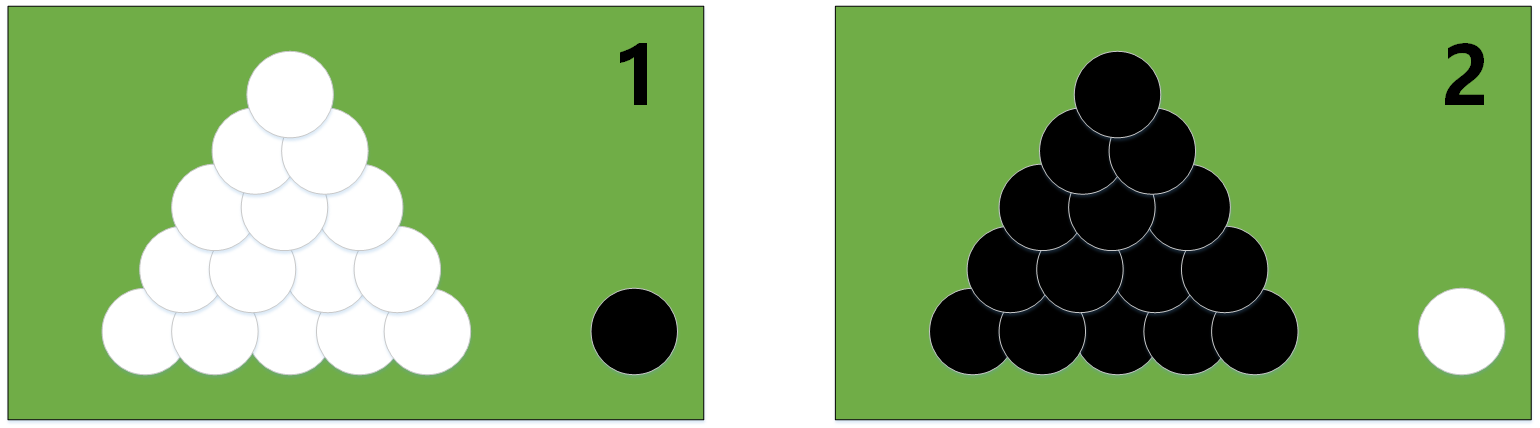
\includegraphics{./img/ch2/2.19.1.1.png}
 
% \end{figure}

​
例:有两个外形完全相同的箱子,1号箱有99只白球,1只黑球;2号箱有1只白球,99只黑球。在一次实验中,取出的是黑球,请问是从哪个箱子中取出的?

​
一般的根据经验想法,会猜测这只黑球最像是从2号箱取出,此时描述的``最像''就有``最大似然''的意思,这种想法常称为``最大似然原理''。

\subsection{极大似然估计原理}\label{ux6781ux5927ux4f3cux7136ux4f30ux8ba1ux539fux7406}

​
总结起来,最大似然估计的目的就是:利用已知的样本结果,反推最有可能(最大概率)导致这样结果的参数值。

​
极大似然估计是建立在极大似然原理的基础上的一个统计方法。极大似然估计提供了一种给定观察数据来评估模型参数的方法,即:``模型已定,参数未知''。通过若干次试验,观察其结果,利用试验结果得到某个参数值能够使样本出现的概率为最大,则称为极大似然估计。

​
由于样本集中的样本都是独立同分布,可以只考虑一类样本集$D$,来估计参数向量$\vec\theta$。记已知的样本集为:
\[
D=\vec x_{1},\vec x_{2},...,\vec x_{n}
\] 似然函数(likelihood
function):联合概率密度函数$p(D|\vec\theta )$称为相对于$\vec x_{1},\vec x_{2},...,\vec x_{n}$的$\vec\theta$的似然函数。
\[
l(\vec\theta )=p(D|\vec\theta ) =p(\vec x_{1},\vec x_{2},...,\vec x_{n}|\vec\theta )=\prod_{i=1}^{n}p(\vec x_{i}|\vec \theta )
\]
如果$\hat{\vec\theta}$是参数空间中能使似然函数$l(\vec\theta)$最大的$\vec\theta$值,则$\hat{\vec\theta}$应该是``最可能''的参数值,那么$\hat{\vec\theta}​$就是$\theta$的极大似然估计量。它是样本集的函数,记作:
\[
\hat{\vec\theta}=d(D)= \mathop {\arg \max}_{\vec\theta} l(\vec\theta )
\]
$\hat{\vec\theta}(\vec x_{1},\vec x_{2},...,\vec x_{n})$称为极大似然函数估计值。

\subsection{贝叶斯分类器基本原理}\label{ux8d1dux53f6ux65afux5206ux7c7bux5668ux57faux672cux539fux7406}

​
贝叶斯决策论通过\textbf{相关概率已知}的情况下利用\textbf{误判损失}来选择最优的类别分类。\\
假设有$N$种可能的分类标记,记为$Y={c_1,c_2,...,c_N}$,那对于样本$\boldsymbol{x}$,它属于哪一类呢?

计算步骤如下:

step 1. 算出样本$\boldsymbol{x}$属于第i个类的概率,即$P(c_i|x)​$;

step 2.
通过比较所有的$P(c_i|\boldsymbol{x})$,得到样本$\boldsymbol{x}$所属的最佳类别。

step 3. 将类别$c_i$和样本$\boldsymbol{x}$代入到贝叶斯公式中,得到:
\[
P(c_i|\boldsymbol{x})=\frac{P(\boldsymbol{x}|c_i)P(c_i)}{P(\boldsymbol{x})}.
\] ​
一般来说,$P(c_i)$为先验概率,$P(\boldsymbol{x}|c_i)$为条件概率,$P(\boldsymbol{x})$是用于归一化的证据因子。对于$P(c_i)$可以通过训练样本中类别为$c_i$的样本所占的比例进行估计;此外,由于只需要找出最大的$P(\boldsymbol{x}|c_i)$,因此我们并不需要计算$P(\boldsymbol{x})$。\\
​
为了求解条件概率,基于不同假设提出了不同的方法,以下将介绍朴素贝叶斯分类器和半朴素贝叶斯分类器。

\subsection{朴素贝叶斯分类器}\label{ux6734ux7d20ux8d1dux53f6ux65afux5206ux7c7bux5668}

​
假设样本$\boldsymbol{x}$包含$d$个属性,即$\boldsymbol{x}={ x_1,x_2,...,x_d}$。于是有:
\[
P(\boldsymbol{x}|c_i)=P(x_1,x_2,\cdots,x_d|c_i)
\]
这个联合概率难以从有限的训练样本中直接估计得到。于是,朴素贝叶斯(Naive
Bayesian,简称NB)采用了``属性条件独立性假设'':对已知类别,假设所有属性相互独立。于是有:
\[
P(x_1,x_2,\cdots,x_d|c_i)=\prod_{j=1}^d P(x_j|c_i)
\] 这样的话,我们就可以很容易地推出相应的判定准则了: \[
h_{nb}(\boldsymbol{x})=\mathop{\arg \max}_{c_i\in Y} P(c_i)\prod_{j=1}^dP(x_j|c_i)
\] \textbf{条件概率$P(x_j|c_i)​$的求解}

如果$x_j$是标签属性,那么我们可以通过计数的方法估计$P(x_j|c_i)$ \[
P(x_j|c_i)=\frac{P(x_j,c_i)}{P(c_i)}\approx\frac{\#(x_j,c_i)}{\#(c_i)}
\]
其中,$\#(x_j,c_i)$表示在训练样本中$x_j$与$c_{i}$共同出现的次数。

如果$x_j​$是数值属性,通常我们假设类别中$c_{i}​$的所有样本第$j​$个属性的值服从正态分布。我们首先估计这个分布的均值$μ​$和方差$σ​$,然后计算$x_j​$在这个分布中的概率密度$P(x_j|c_i)​$。

\subsection{举例理解朴素贝叶斯分类器}\label{ux4e3eux4f8bux7406ux89e3ux6734ux7d20ux8d1dux53f6ux65afux5206ux7c7bux5668}

使用经典的西瓜训练集如下:

\begin{longtable}[]{ cccccccccc }
%\toprule
编号 & 色泽 & 根蒂 & 敲声 & 纹理 & 脐部 & 触感 & 密度 & 含糖率 &
好瓜\tabularnewline
%\midrule
%\endhead
1 & 青绿 & 蜷缩 & 浊响 & 清晰 & 凹陷 & 硬滑 & 0.697 & 0.460 &
是\tabularnewline
2 & 乌黑 & 蜷缩 & 沉闷 & 清晰 & 凹陷 & 硬滑 & 0.774 & 0.376 &
是\tabularnewline
3 & 乌黑 & 蜷缩 & 浊响 & 清晰 & 凹陷 & 硬滑 & 0.634 & 0.264 &
是\tabularnewline
4 & 青绿 & 蜷缩 & 沉闷 & 清晰 & 凹陷 & 硬滑 & 0.608 & 0.318 &
是\tabularnewline
5 & 浅白 & 蜷缩 & 浊响 & 清晰 & 凹陷 & 硬滑 & 0.556 & 0.215 &
是\tabularnewline
6 & 青绿 & 稍蜷 & 浊响 & 清晰 & 稍凹 & 软粘 & 0.403 & 0.237 &
是\tabularnewline
7 & 乌黑 & 稍蜷 & 浊响 & 稍糊 & 稍凹 & 软粘 & 0.481 & 0.149 &
是\tabularnewline
8 & 乌黑 & 稍蜷 & 浊响 & 清晰 & 稍凹 & 硬滑 & 0.437 & 0.211 &
是\tabularnewline
9 & 乌黑 & 稍蜷 & 沉闷 & 稍糊 & 稍凹 & 硬滑 & 0.666 & 0.091 &
否\tabularnewline
10 & 青绿 & 硬挺 & 清脆 & 清晰 & 平坦 & 软粘 & 0.243 & 0.267 &
否\tabularnewline
11 & 浅白 & 硬挺 & 清脆 & 模糊 & 平坦 & 硬滑 & 0.245 & 0.057 &
否\tabularnewline
12 & 浅白 & 蜷缩 & 浊响 & 模糊 & 平坦 & 软粘 & 0.343 & 0.099 &
否\tabularnewline
13 & 青绿 & 稍蜷 & 浊响 & 稍糊 & 凹陷 & 硬滑 & 0.639 & 0.161 &
否\tabularnewline
14 & 浅白 & 稍蜷 & 沉闷 & 稍糊 & 凹陷 & 硬滑 & 0.657 & 0.198 &
否\tabularnewline
15 & 乌黑 & 稍蜷 & 浊响 & 清晰 & 稍凹 & 软粘 & 0.360 & 0.370 &
否\tabularnewline
16 & 浅白 & 蜷缩 & 浊响 & 模糊 & 平坦 & 硬滑 & 0.593 & 0.042 &
否\tabularnewline
17 & 青绿 & 蜷缩 & 沉闷 & 稍糊 & 稍凹 & 硬滑 & 0.719 & 0.103 &
否\tabularnewline
% \bottomrule
\end{longtable}

对下面的测试例``测1''进行 分类:

\begin{longtable}[]{ cccccccccc }
%\toprule
编号 & 色泽 & 根蒂 & 敲声 & 纹理 & 脐部 & 触感 & 密度 & 含糖率 &
好瓜\tabularnewline
%\midrule
%\endhead
测1 & 青绿 & 蜷缩 & 浊响 & 清晰 & 凹陷 & 硬滑 & 0.697 & 0.460 &
?\tabularnewline
% \bottomrule
\end{longtable}

首先,估计类先验概率$P(c_j)$,有 \[
\begin{align} 
&P(好瓜=是)=\frac{8}{17}=0.471 \newline 
&P(好瓜=否)=\frac{9}{17}=0.529 
\end{align}
\]
然后,为每个属性估计条件概率(这里,对于连续属性,假定它们服从正态分布)
\[
P_{青绿|是}=P(色泽=青绿|好瓜=是)=\frac{3}{8}=0.375
\]

\[
P_{青绿|否}=P(色泽=青绿|好瓜=否)=\frac{3}{9}\approx0.333
\]

\[
P_{蜷缩|是}=P(根蒂=蜷缩|好瓜=是)=\frac{5}{8}=0.625
\]

\[
P_{蜷缩|否}=P(根蒂=蜷缩|好瓜=否)=\frac{3}{9}=0.333
\]

\[
P_{浊响|是}=P(敲声=浊响|好瓜=是)=\frac{6}{8}=0.750
\]

\[
P_{浊响|否}=P(敲声=浊响|好瓜=否)=\frac{4}{9}\approx 0.444
\]

\[
P_{清晰|是}=P(纹理=清晰|好瓜=是)=\frac{7}{8}= 0.875
\]

\[
P_{清晰|否}=P(纹理=清晰|好瓜=否)=\frac{2}{9}\approx 0.222
\]

\[
P_{凹陷|是}=P(脐部=凹陷|好瓜=是)=\frac{6}{8}= 0.750
\]

\[
P_{凹陷|否}=P(脐部=凹陷|好瓜=否)=\frac{2}{9} \approx 0.222
\]

\[
P_{硬滑|是}=P(触感=硬滑|好瓜=是)=\frac{6}{8}= 0.750
\]

\[
P_{硬滑|否}=P(触感=硬滑|好瓜=否)=\frac{6}{9} \approx 0.667
\]

\[
\begin{aligned}
\rho_{密度:0.697|是}&=\rho(密度=0.697|好瓜=是)\\&=\frac{1}{\sqrt{2 \pi}\times0.129}exp\left( -\frac{(0.697-0.574)^2}{2\times0.129^2}\right) \approx 1.959
\end{aligned}
\]

\[
\begin{aligned}
\rho_{密度:0.697|否}&=\rho(密度=0.697|好瓜=否)\\&=\frac{1}{\sqrt{2 \pi}\times0.195}exp\left( -\frac{(0.697-0.496)^2}{2\times0.195^2}\right) \approx 1.203
\end{aligned}
\]

\[
\begin{aligned}
\rho_{含糖:0.460|是}&=\rho(密度=0.460|好瓜=是)\\&=\frac{1}{\sqrt{2 \pi}\times0.101}exp\left( -\frac{(0.460-0.279)^2}{2\times0.101^2}\right) \approx 0.788
\end{aligned}
\]

\[
\begin{aligned}
\rho_{含糖:0.460|否}&=\rho(密度=0.460|好瓜=是)\\&=\frac{1}{\sqrt{2 \pi}\times0.108}exp\left( -\frac{(0.460-0.154)^2}{2\times0.108^2}\right) \approx 0.066
\end{aligned}
\]

于是有 \[
\begin{align} 
P(&好瓜=是)\times P_{青绿|是} \times P_{蜷缩|是} \times P_{浊响|是} \times P_{清晰|是} \times P_{凹陷|是}\newline 
&\times P_{硬滑|是} \times p_{密度:0.697|是} \times p_{含糖:0.460|是} \approx 0.063 \newline\newline 
P(&好瓜=否)\times P_{青绿|否} \times P_{蜷缩|否} \times P_{浊响|否} \times P_{清晰|否} \times P_{凹陷|否}\newline 
&\times P_{硬滑|否} \times p_{密度:0.697|否} \times p_{含糖:0.460|否} \approx 6.80\times 10^{-5} 
\end{align}
\]

由于$0.063>6.80\times 10^{-5}$,因此,朴素贝叶斯分类器将测试样本``测1''判别为``好瓜''。

\subsection{半朴素贝叶斯分类器}\label{ux534aux6734ux7d20ux8d1dux53f6ux65afux5206ux7c7bux5668}

​
朴素贝叶斯采用了``属性条件独立性假设'',半朴素贝叶斯分类器的基本想法是适当考虑一部分属性间的相互依赖信息。\textbf{独依赖估计}(One-Dependence
Estimator,简称ODE)是半朴素贝叶斯分类器最常用的一种策略。顾名思义,独依赖是假设每个属性在类别之外最多依赖一个其他属性,即:
\[
P(\boldsymbol{x}|c_i)=\prod_{j=1}^d P(x_j|c_i,{\rm pa}_j)
\]
其中$pa_j$为属性$x_i$所依赖的属性,成为$x_i$的父属性。假设父属性$pa_j$已知,那么可以使用下面的公式估计$P(x_j|c_i,{\rm pa}_j)$
\[
P(x_j|c_i,{\rm pa}_j)=\frac{P(x_j,c_i,{\rm pa}_j)}{P(c_i,{\rm pa}_j)}
\]

\section{ EM算法}\label{emux7b97ux6cd5}

\subsection{EM算法基本思想}\label{emux7b97ux6cd5ux57faux672cux601dux60f3}

​ 最大期望算法(Expectation-Maximization algorithm,
EM),是一类通过迭代进行极大似然估计的优化算法,通常作为牛顿迭代法的替代,用于对包含隐变量或缺失数据的概率模型进行参数估计。

​ 最大期望算法基本思想是经过两个步骤交替进行计算:

​
第一步是计算期望(E),利用对隐藏变量的现有估计值,计算其最大似然估计值\textbf{;}

​ 第二步是最大化(M),最大化在E步上求得的最大似然值来计算参数的值。

​ M步上找到的参数估计值被用于下一个E步计算中,这个过程不断交替进行。

\subsection{EM算法推导}\label{emux7b97ux6cd5ux63a8ux5bfc}

​
对于$m$个样本观察数据$x=(x^{1},x^{2},...,x^{m})$,现在想找出样本的模型参数$\theta$,其极大化模型分布的对数似然函数为:
\[
\theta = \mathop{\arg\max}_\theta\sum\limits_{i=1}^m logP(x^{(i)};\theta)
\]
如果得到的观察数据有未观察到的隐含数据$z=(z^{(1)},z^{(2)},...z^{(m)})$,极大化模型分布的对数似然函数则为:
\[
\theta =\mathop{\arg\max}_\theta\sum\limits_{i=1}^m logP(x^{(i)};\theta) = \mathop{\arg\max}_\theta\sum\limits_{i=1}^m log\sum\limits_{z^{(i)}}P(x^{(i)}, z^{(i)};\theta)  \tag{a}
\] 由于上式不能直接求出$\theta$,采用缩放技巧: \[
\begin{align} \sum\limits_{i=1}^m log\sum\limits_{z^{(i)}}P(x^{(i)}, z^{(i)};\theta)   & = \sum\limits_{i=1}^m log\sum\limits_{z^{(i)}}Q_i(z^{(i)})\frac{P(x^{(i)}, z^{(i)};\theta)}{Q_i(z^{(i)})} \\ & \geqslant  \sum\limits_{i=1}^m \sum\limits_{z^{(i)}}Q_i(z^{(i)})log\frac{P(x^{(i)}, z^{(i)};\theta)}{Q_i(z^{(i)})} \end{align}   \tag{1}
\] 上式用到了Jensen不等式: \[
log\sum\limits_j\lambda_jy_j \geqslant \sum\limits_j\lambda_jlogy_j\;\;,  \lambda_j \geqslant 0, \sum\limits_j\lambda_j =1
\] 并且引入了一个未知的新分布$Q_i(z^{(i)})$。

此时,如果需要满足Jensen不等式中的等号,所以有: \[
\frac{P(x^{(i)}, z^{(i)};\theta)}{Q_i(z^{(i)})} =c, c为常数
\] 由于$Q_i(z^{(i)})$是一个分布,所以满足 \[
\sum\limits_{z}Q_i(z^{(i)}) =1
\] 综上,可得: \[
Q_i(z^{(i)})  = \frac{P(x^{(i)}, z^{(i)};\theta)}{\sum\limits_{z}P(x^{(i)}, z^{(i)};\theta)} =  \frac{P(x^{(i)}, z^{(i)};\theta)}{P(x^{(i)};\theta)} = P( z^{(i)}|x^{(i)};\theta)
\] 如果$Q_i(z^{(i)}) = P( z^{(i)}|x^{(i)};\theta)$
,则第(1)式是我们的包含隐藏数据的对数似然的一个下界。如果我们能极大化这个下界,则也在尝试极大化我们的对数似然。即我们需要最大化下式:
\[
\mathop{\arg\max}_\theta \sum\limits_{i=1}^m \sum\limits_{z^{(i)}}Q_i(z^{(i)})log\frac{P(x^{(i)}, z^{(i)};\theta)}{Q_i(z^{(i)})}
\] 简化得: \[
\mathop{\arg\max}_\theta \sum\limits_{i=1}^m \sum\limits_{z^{(i)}}Q_i(z^{(i)})log{P(x^{(i)}, z^{(i)};\theta)}
\]
以上即为EM算法的M步,$\sum\limits_{z^{(i)}}Q_i(z^{(i)})log{P(x^{(i)}, z^{(i)};\theta)}​$可理解为$logP(x^{(i)},
z^{(i)};\theta) $基于条件概率分布$Q\_i(z^{(i)})
$的期望。以上即为EM算法中E步和M步的具体数学含义。

\subsection{ 图解EM算法}\label{ux56feux89e3emux7b97ux6cd5}

​
考虑上一节中的(a)式,表达式中存在隐变量,直接找到参数估计比较困难,通过EM算法迭代求解下界的最大值到收敛为止。

% \begin{figure}
% \centering
% 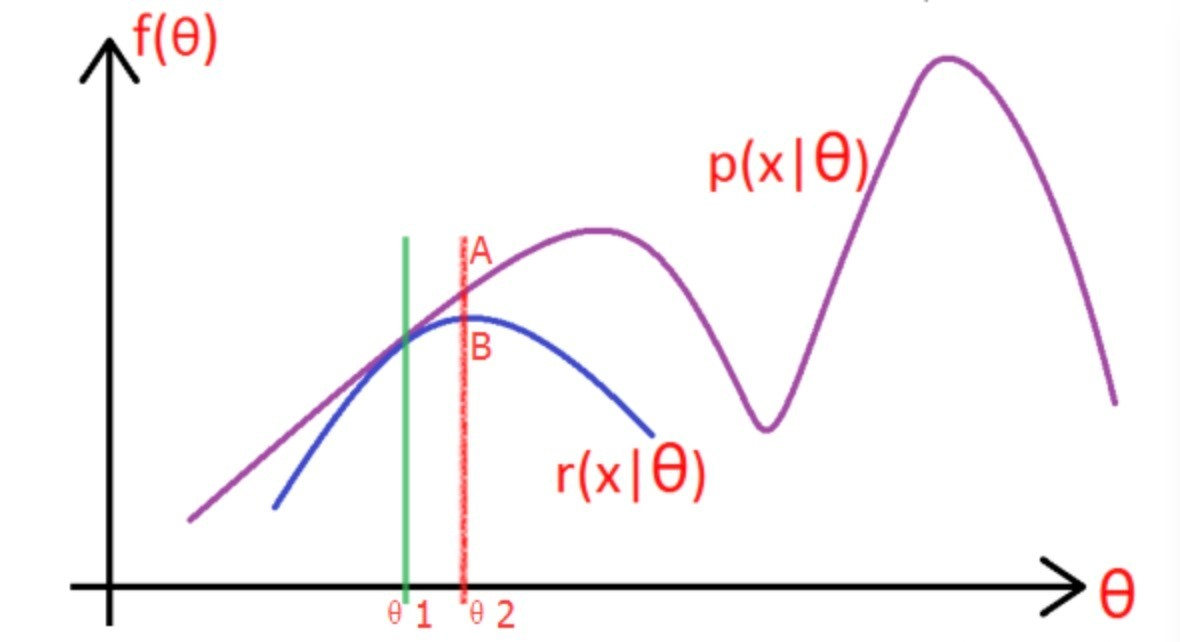
\includegraphics{./img/ch2/2.20.1.jpg}
 
% \end{figure}

​
图片中的紫色部分是我们的目标模型$p(x|\theta)$,该模型复杂,难以求解析解,为了消除隐变量$z^{(i)}$的影响,我们可以选择一个不包含$z^{(i)}$的模型$r(x|\theta)$,使其满足条件$r(x\textbar{}\theta)
\leqslant p(x\textbar{}\theta) $。

求解步骤如下:

(1)选取$\theta_1$,使得$r(x|\theta_1) = p(x|\theta_1)$,然后对此时的$r$求取最大值,得到极值点$\theta_2$,实现参数的更新。

(2)重复以上过程到收敛为止,在更新过程中始终满足$r \leqslant p $.

\subsection{ EM算法流程}\label{emux7b97ux6cd5ux6d41ux7a0b}

输入:观察数据$x=(x^{(1)},x^{(2)},...x^{(m)})$,联合分布$p(x,z ;\theta)$,条件分布$p(z|x; \theta)$,最大迭代次数$J$

1)随机初始化模型参数$\theta$的初值$\theta^0$。

2)$for \ j \ from \ 1 \ to \ j$:

​ a) E步。计算联合分布的条件概率期望: \[
Q_i(z^{(i)}) = P( z^{(i)}|x^{(i)}, \theta^{j})
\]

\[
L(\theta, \theta^{j}) = \sum\limits_{i=1}^m\sum\limits_{z^{(i)}}P( z^{(i)}|x^{(i)}, \theta^{j})log{P(x^{(i)}, z^{(i)};\theta)}
\]

​ b) M步。极大化$L(\theta, \theta^{j})$,得到$\theta^{j+1}$: \[
\theta^{j+1} = \mathop{\arg\max}_\theta L(\theta, \theta^{j})
\] ​ c)
如果$\theta^{j+1}$收敛,则算法结束。否则继续回到步骤a)进行E步迭代。

输出:模型参数$\theta​$。

\section{ 降维和聚类}\label{ux964dux7ef4ux548cux805aux7c7b}

\subsection{图解为什么会产生维数灾难}\label{ux56feux89e3ux4e3aux4ec0ux4e48ux4f1aux4ea7ux751fux7ef4ux6570ux707eux96be}

​
假如数据集包含10张照片,照片中包含三角形和圆两种形状。现在来设计一个分类器进行训练,让这个分类器对其他的照片进行正确分类(假设三角形和圆的总数是无限大),简单的,我们用一个特征进行分类:

% \begin{figure}
% \centering
% 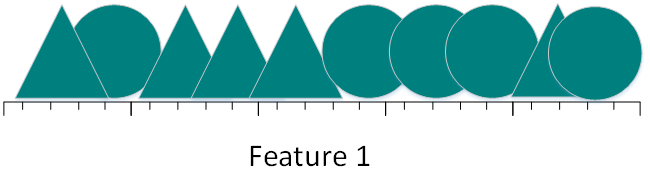
\includegraphics{./img/ch2/2.21.1.1.png}
 
% \end{figure}

​ 图2.21.1.a

​
从上图可看到,如果仅仅只有一个特征进行分类,三角形和圆几乎是均匀分布在这条线段上,很难将10张照片线性分类。那么,增加一个特征后的情况会怎么样:

% \begin{figure}
% \centering
% 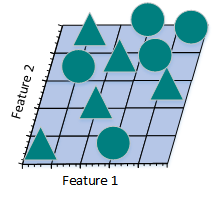
\includegraphics{./img/ch2/2.21.1.2.png}
 
% \end{figure}

​ 图2.21.1.b

增加一个特征后,我们发现仍然无法找到一条直线将猫和狗分开。所以,考虑需要再增加一个特征:

% \begin{figure}
% \centering
% 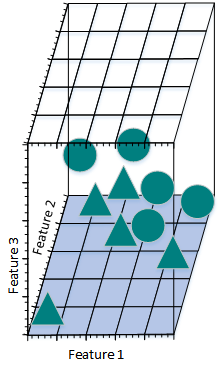
\includegraphics{./img/ch2/2.21.1.3.png}
 
% \end{figure}

​ 图2.21.1.c

% \begin{figure}
% \centering
% 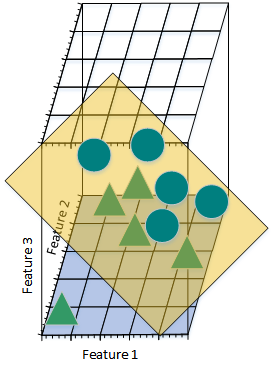
\includegraphics{./img/ch2/2.21.1.4.png}
 
% \end{figure}

​ 图2.21.1.d

​ 此时,可以找到一个平面将三角形和圆分开。

​ 现在计算一下不同特征数是样本的密度:

​
(1)一个特征时,假设特征空间时长度为5的线段,则样本密度为$10 \div 5 = 2$。

​ (2)两个特征时,特征空间大小为$ 5\times5 =
25$,样本密度为$10 \div 25 = 0.4$。

​ (3)三个特征时,特征空间大小是$ 5\times5\times5 =
125$,样本密度为$10 \div 125 = 0.08$。

​
以此类推,如果继续增加特征数量,样本密度会越来越稀疏,此时,更容易找到一个超平面将训练样本分开。当特征数量增长至无限大时,样本密度就变得非常稀疏。

​ 下面看一下将高维空间的分类结果映射到低维空间时,会出现什么情况?

\begin{figure}
\centering
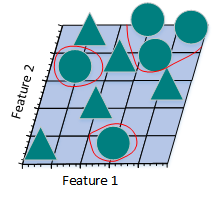
\includegraphics{./img/ch2/2.21.1.5.png}
 
\end{figure}

​ 图2.21.1.e

​
上图是将三维特征空间映射到二维特征空间后的结果。尽管在高维特征空间时训练样本线性可分,但是映射到低维空间后,结果正好相反。事实上,增加特征数量使得高维空间线性可分,相当于在低维空间内训练一个复杂的非线性分类器。不过,这个非线性分类器太过``聪明'',仅仅学到了一些特例。如果将其用来辨别那些未曾出现在训练样本中的测试样本时,通常结果不太理想,会造成过拟合问题。

% \begin{figure}
% \centering
% 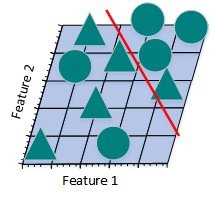
\includegraphics{./img/ch2/2.21.1.6a.png}
 
% \end{figure}

​ 图2.21.1.f

​
上图所示的只采用2个特征的线性分类器分错了一些训练样本,准确率似乎没有图2.21.1.e的高,但是,采用2个特征的线性分类器的泛化能力比采用3个特征的线性分类器要强。因为,采用2个特征的线性分类器学习到的不只是特例,而是一个整体趋势,对于那些未曾出现过的样本也可以比较好地辨别开来。换句话说,通过减少特征数量,可以避免出现过拟合问题,从而避免``维数灾难''。

% \begin{figure}
% \centering
% 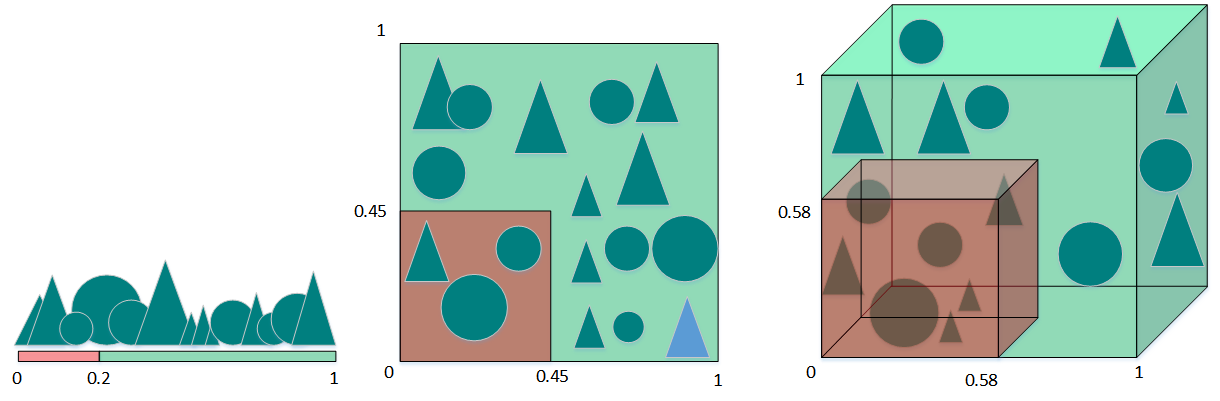
\includegraphics{./img/ch2/2.21.1.6.png}
 
% \end{figure}

​
上图从另一个角度诠释了``维数灾难''。假设只有一个特征时,特征的值域是0到1,每一个三角形和圆的特征值都是唯一的。如果我们希望训练样本覆盖特征值值域的20\%,那么就需要三角形和圆总数的20\%。我们增加一个特征后,为了继续覆盖特征值值域的20\%就需要三角形和圆总数的45\%($0.452^2\approx0.2$)。继续增加一个特征后,需要三角形和圆总数的58\%($0.583^3\approx0.2$)。随着特征数量的增加,为了覆盖特征值值域的20\%,就需要更多的训练样本。如果没有足够的训练样本,就可能会出现过拟合问题。

​
通过上述例子,我们可以看到特征数量越多,训练样本就会越稀疏,分类器的参数估计就会越不准确,更加容易出现过拟合问题。``维数灾难''的另一个影响是训练样本的稀疏性并不是均匀分布的。处于中心位置的训练样本比四周的训练样本更加稀疏。

% \begin{figure}
% \centering
% 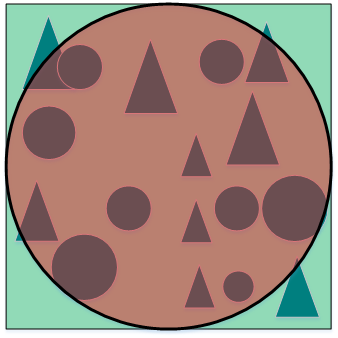
\includegraphics{./img/ch2/2.21.1.7.png}
 
% \end{figure}

​
假设有一个二维特征空间,如上图所示的矩形,在矩形内部有一个内切的圆形。由于越接近圆心的样本越稀疏,因此,相比于圆形内的样本,那些位于矩形四角的样本更加难以分类。当维数变大时,特征超空间的容量不变,但单位圆的容量会趋于0,在高维空间中,大多数训练数据驻留在特征超空间的角落。散落在角落的数据要比处于中心的数据难于分类。

\subsection{怎样避免维数灾难}\label{ux600eux6837ux907fux514dux7ef4ux6570ux707eux96be}

\textbf{有待完善!!!}

解决维度灾难问题:

主成分分析法PCA,线性判别法LDA

奇异值分解简化数据、拉普拉斯特征映射

Lassio缩减系数法、小波分析法、

\subsection{聚类和降维有什么区别与联系}\label{ux805aux7c7bux548cux964dux7ef4ux6709ux4ec0ux4e48ux533aux522bux4e0eux8054ux7cfb}

​
聚类用于找寻数据内在的分布结构,既可以作为一个单独的过程,比如异常检测等等。也可作为分类等其他学习任务的前驱过程。聚类是标准的无监督学习。

​
1)在一些推荐系统中需确定新用户的类型,但定义``用户类型''却可能不太容易,此时往往可先对原有的用户数据进行聚类,根据聚类结果将每个簇定义为一个类,然后再基于这些类训练分类模型,用于判别新用户的类型。

% \begin{figure}
% \centering
% 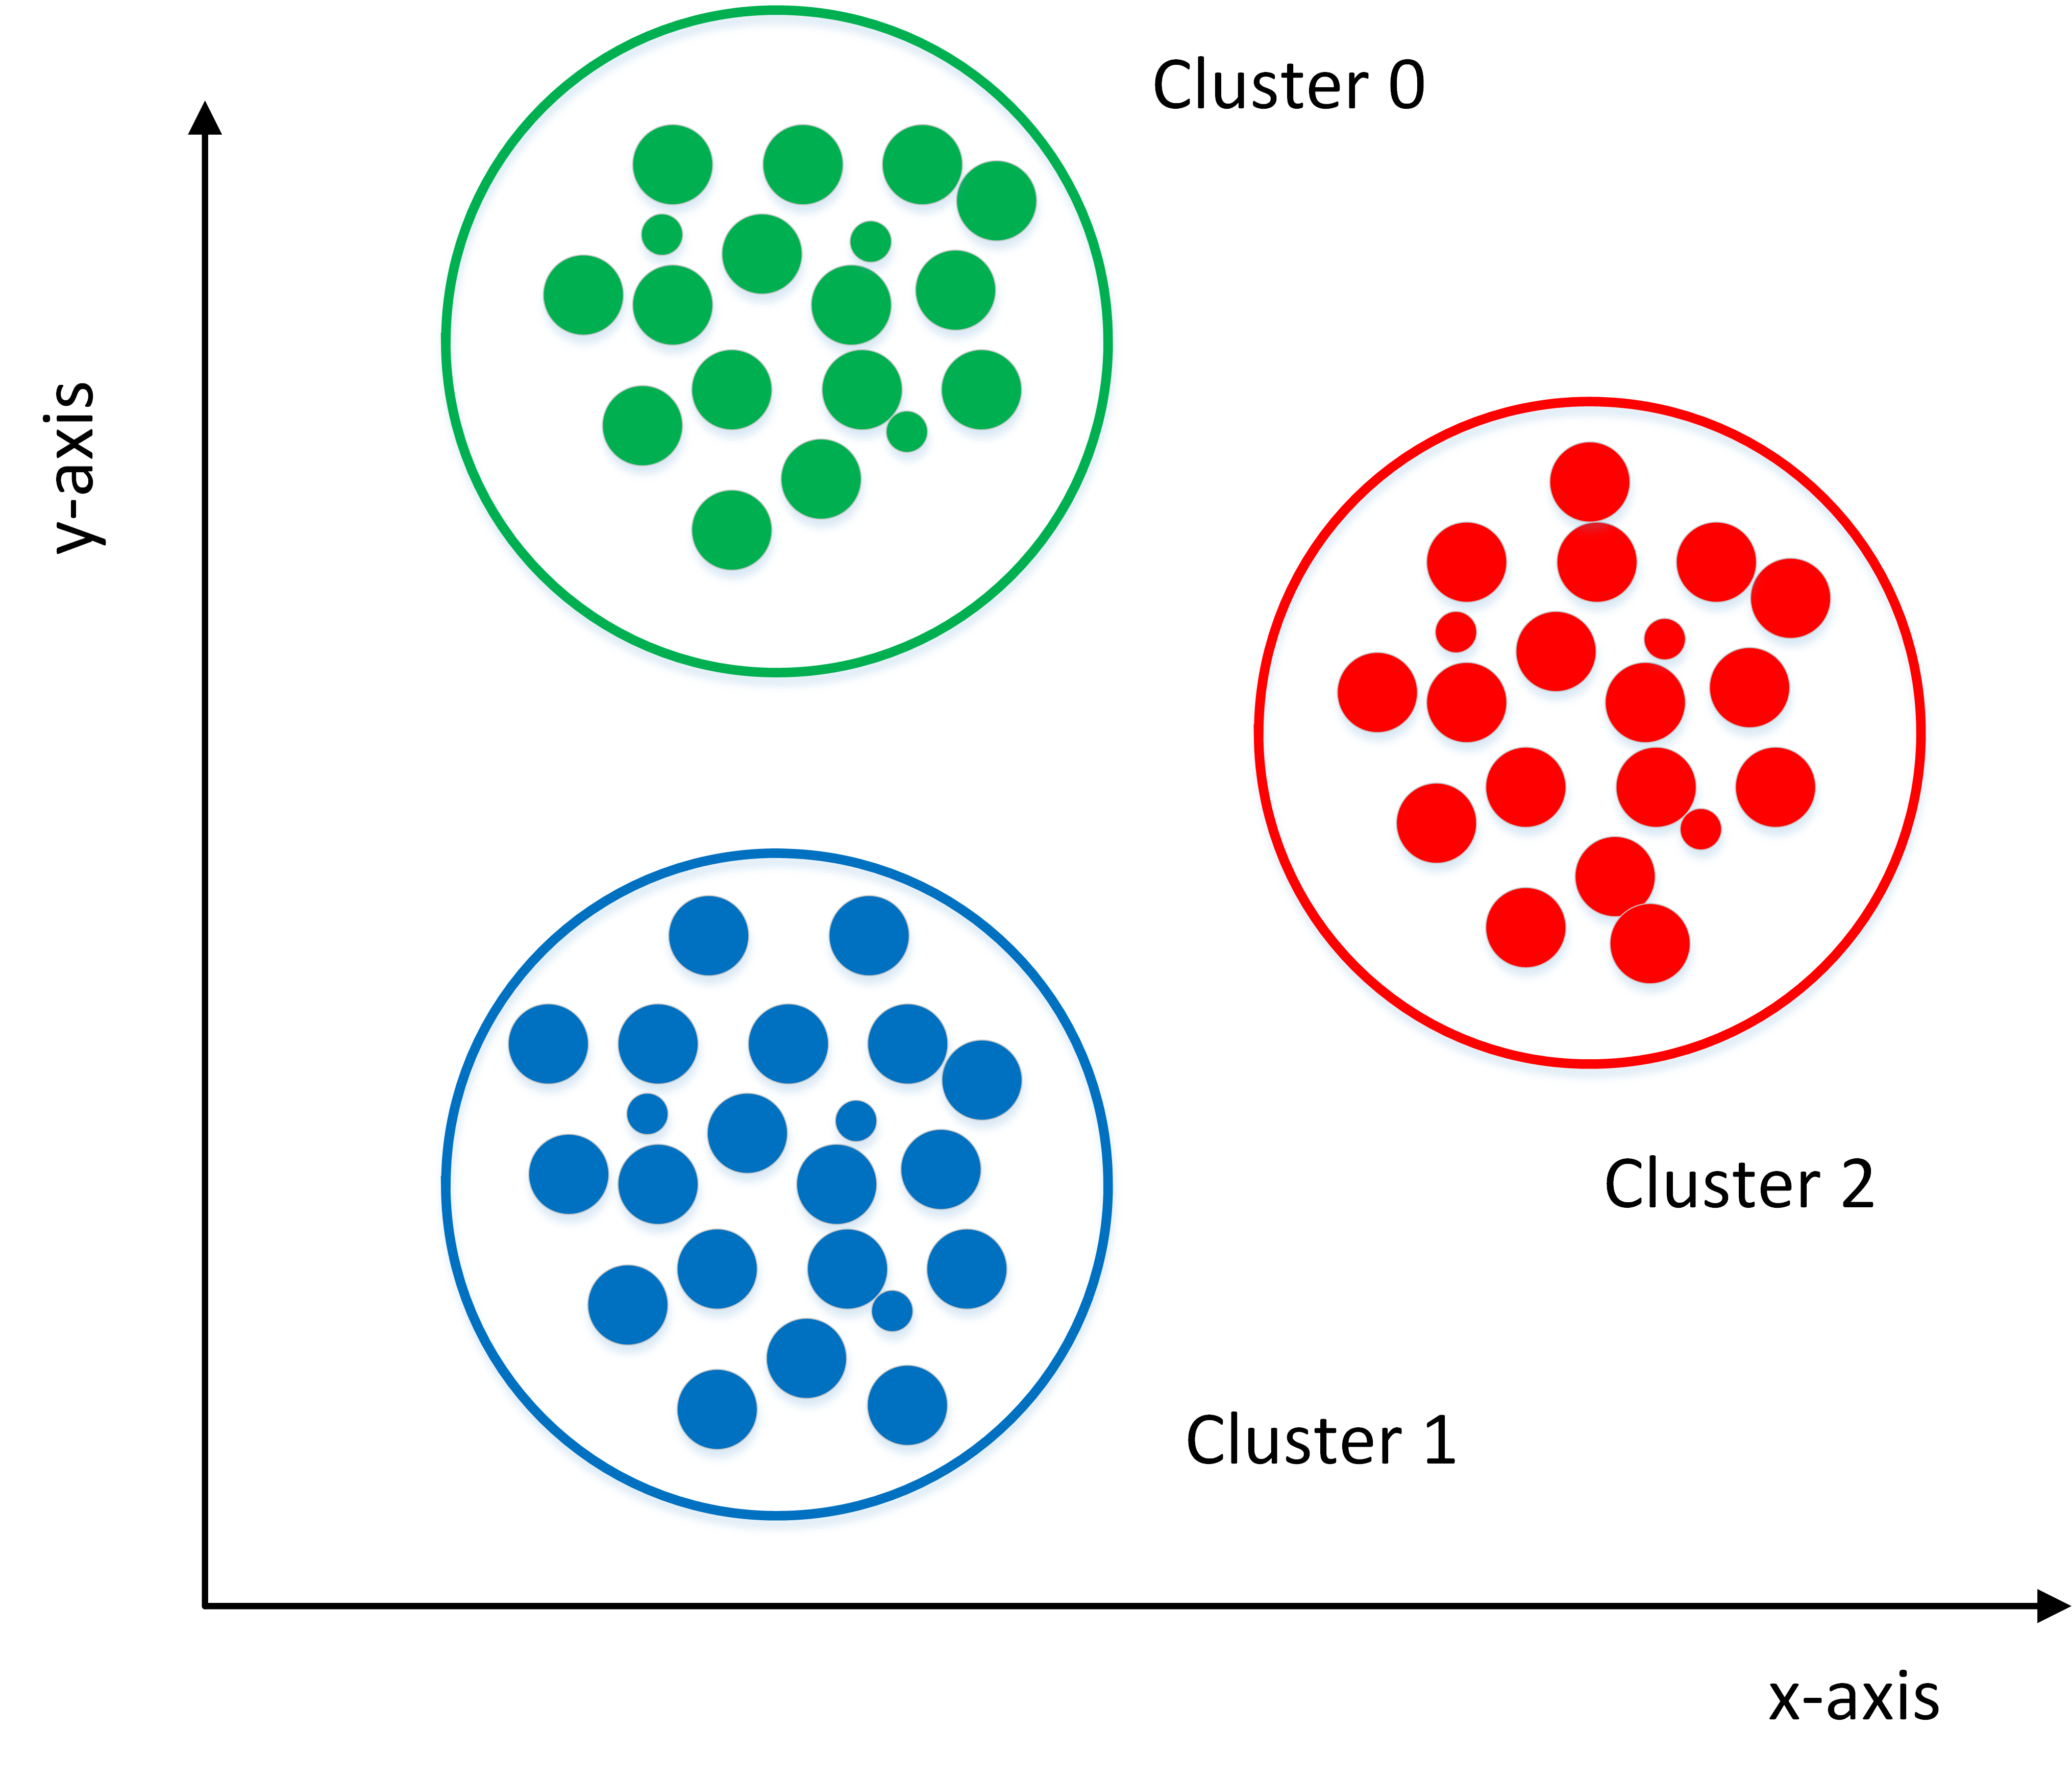
\includegraphics{./img/ch2/2.21.3.1.png}
 
% \end{figure}

​
2)而降维则是为了缓解维数灾难的一个重要方法,就是通过某种数学变换将原始高维属性空间转变为一个低维``子空间''。其基于的假设就是,虽然人们平时观测到的数据样本虽然是高维的,但是实际上真正与学习任务相关的是个低维度的分布。从而通过最主要的几个特征维度就可以实现对数据的描述,对于后续的分类很有帮助。比如对于Kaggle(数据分析竞赛平台之一)上的泰坦尼克号生还问题。通过给定一个乘客的许多特征如年龄、姓名、性别、票价等,来判断其是否能在海难中生还。这就需要首先进行特征筛选,从而能够找出主要的特征,让学习到的模型有更好的泛化性。

​ 聚类和降维都可以作为分类等问题的预处理步骤。

% \begin{figure}
% \centering
% 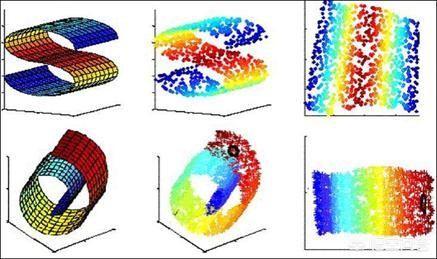
\includegraphics{./img/ch2/2-19.jpg}
 
% \end{figure}

​
但是他们虽然都能实现对数据的约减。但是二者适用的对象不同,聚类针对的是数据点,而降维则是对于数据的特征。另外它们有着很多种实现方法。聚类中常用的有K-means、层次聚类、基于密度的聚类等;降维中常用的则PCA、Isomap、LLE等。

\subsection{有哪些聚类算法优劣衡量标准}\label{ux6709ux54eaux4e9bux805aux7c7bux7b97ux6cd5ux4f18ux52a3ux8861ux91cfux6807ux51c6}

不同聚类算法有不同的优劣和不同的适用条件。可从以下方面进行衡量判断:
1、算法的处理能力:处理大的数据集的能力,即算法复杂度;处理数据噪声的能力;处理任意形状,包括有间隙的嵌套的数据的能力;
2、算法是否需要预设条件:是否需要预先知道聚类个数,是否需要用户给出领域知识;

​
3、算法的数据输入属性:算法处理的结果与数据输入的顺序是否相关,也就是说算法是否独立于数据输入顺序;算法处理有很多属性数据的能力,也就是对数据维数是否敏感,对数据的类型有无要求。

\subsection{聚类和分类有什么区别}\label{ux805aux7c7bux548cux5206ux7c7bux6709ux4ec0ux4e48ux533aux522b}

\textbf{聚类(Clustering) }
聚类,简单地说就是把相似的东西分到一组,聚类的时候,我们并不关心某一类是什么,我们需要实现的目标只是把相似的东西聚到一起。一个聚类算法通常只需要知道如何计算相似度就可以开始工作了,因此聚类通常并不需要使用训练数据进行学习,在机器学习中属于无监督学习。

\textbf{分类(Classification) }

​
分类,对于一个分类器,通常需要你告诉它``这个东西被分为某某类''。一般情况下,一个分类器会从它得到的训练集中进行学习,从而具备对未知数据进行分类的能力,在机器学习中属于监督学习。

\subsection{不同聚类算法特点性能比较}\label{ux4e0dux540cux805aux7c7bux7b97ux6cd5ux7279ux70b9ux6027ux80fdux6bd4ux8f83}

\begin{longtable}[]{ ccccccc }
%\toprule
算法名称 & 可伸缩性 & 适合的数据类型 & 高维性 & 异常数据抗干扰性 &
聚类形状 & 算法效率\tabularnewline
%\midrule
%\endhead
WAVECLUSTER & 很高 & 数值型 & 很高 & 较高 & 任意形状 &
很高\tabularnewline
ROCK & 很高 & 混合型 & 很高 & 很高 & 任意形状 & 一般\tabularnewline
BIRCH & 较高 & 数值型 & 较低 & 较低 & 球形 & 很高\tabularnewline
CURE & 较高 & 数值型 & 一般 & 很高 & 任意形状 & 较高\tabularnewline
K-PROTOTYPES & 一般 & 混合型 & 较低 & 较低 & 任意形状 &
一般\tabularnewline
DENCLUE & 较低 & 数值型 & 较高 & 一般 & 任意形状 & 较高\tabularnewline
OPTIGRID & 一般 & 数值型 & 较高 & 一般 & 任意形状 & 一般\tabularnewline
CLIQUE & 较高 & 数值型 & 较高 & 较高 & 任意形状 & 较低\tabularnewline
DBSCAN & 一般 & 数值型 & 较低 & 较高 & 任意形状 & 一般\tabularnewline
CLARANS & 较低 & 数值型 & 较低 & 较高 & 球形 & 较低\tabularnewline
% \bottomrule
\end{longtable}

\subsection{四种常用聚类方法之比较}\label{ux56dbux79cdux5e38ux7528ux805aux7c7bux65b9ux6cd5ux4e4bux6bd4ux8f83}

​
聚类就是按照某个特定标准把一个数据集分割成不同的类或簇,使得同一个簇内的数据对象的相似性尽可能大,同时不在同一个簇中的数据对象的差异性也尽可能地大。即聚类后同一类的数据尽可能聚集到一起,不同类数据尽量分离。
​
主要的聚类算法可以划分为如下几类:划分方法、层次方法、基于密度的方法、基于网格的方法以及基于模型的方法。下面主要对k-means聚类算法、凝聚型层次聚类算法、神经网络聚类算法之SOM,以及模糊聚类的FCM算法通过通用测试数据集进行聚类效果的比较和分析。

\subsection{k-means聚类算法}\label{k-meansux805aux7c7bux7b97ux6cd5}

k-means是划分方法中较经典的聚类算法之一。由于该算法的效率高,所以在对大规模数据进行聚类时被广泛应用。目前,许多算法均围绕着该算法进行扩展和改进。
k-means算法以k为参数,把n个对象分成k个簇,使簇内具有较高的相似度,而簇间的相似度较低。k-means算法的处理过程如下:首先,随机地
选择k个对象,每个对象初始地代表了一个簇的平均值或中心;对剩余的每个对象,根据其与各簇中心的距离,将它赋给最近的簇;然后重新计算每个簇的平均值。
这个过程不断重复,直到准则函数收敛。通常,采用平方误差准则,其定义如下:
\[
E=\sum_{i=1}^{k}\sum_{p\in C_i}\left\|p-m_i\right\|^2
\]
 这里E是数据中所有对象的平方误差的总和,p是空间中的点,$m_i$是簇$C_i$的平均值{[}9{]}。该目标函数使生成的簇尽可能紧凑独立,使用的距离度量是欧几里得距离,当然也可以用其他距离度量。

\textbf{算法流程}: ​ 输入:包含n个对象的数据和簇的数目k; ​
输出:n个对象到k个簇,使平方误差准则最小。 ​ 步骤:   (1)
任意选择k个对象作为初始的簇中心;   (2)
根据簇中对象的平均值,将每个对象(重新)赋予最类似的簇;   (3)
更新簇的平均值,即计算每个簇中对象的平均值;   (4)
重复步骤(2)、(3)直到簇中心不再变化;

\subsection{层次聚类算法}\label{ux5c42ux6b21ux805aux7c7bux7b97ux6cd5}

​
根据层次分解的顺序是自底向上的还是自上向下的,层次聚类算法分为凝聚的层次聚类算法和分裂的层次聚类算法。
 凝聚型层次聚类的策略是先将每个对象作为一个簇,然后合并这些原子簇为越来越大的簇,直到所有对象都在一个簇中,或者某个终结条件被满足。绝大多数层次聚类属于凝聚型层次聚类,它们只是在簇间相似度的定义上有所不同。

\textbf{算法流程}:

注:以采用最小距离的凝聚层次聚类算法为例:

 (1) 将每个对象看作一类,计算两两之间的最小距离;  (2)
将距离最小的两个类合并成一个新类;  (3)
重新计算新类与所有类之间的距离;  (4)
重复(2)、(3),直到所有类最后合并成一类。

\subsection{SOM聚类算法}\label{somux805aux7c7bux7b97ux6cd5}

​
SOM神经网络{[}11{]}是由芬兰神经网络专家Kohonen教授提出的,该算法假设在输入对象中存在一些拓扑结构或顺序,可以实现从输入空间(n维)到输出平面(2维)的降维映射,其映射具有拓扑特征保持性质,与实际的大脑处理有很强的理论联系。

​
SOM网络包含输入层和输出层。输入层对应一个高维的输入向量,输出层由一系列组织在2维网格上的有序节点构成,输入节点与输出节点通过权重向量连接。
学习过程中,找到与之距离最短的输出层单元,即获胜单元,对其更新。同时,将邻近区域的权值更新,使输出节点保持输入向量的拓扑特征。

\textbf{算法流程}:

​ (1) 网络初始化,对输出层每个节点权重赋初值; ​ (2)
从输入样本中随机选取输入向量并且归一化,找到与输入向量距离最小的权重向量;
​ (3) 定义获胜单元,在获胜单元的邻近区域调整权重使其向输入向量靠拢; ​
(4) 提供新样本、进行训练; ​ (5)
收缩邻域半径、减小学习率、重复,直到小于允许值,输出聚类结果。

\subsection{ FCM聚类算法}\label{fcmux805aux7c7bux7b97ux6cd5}

​
1965年美国加州大学柏克莱分校的扎德教授第一次提出了`集合'的概念。经过十多年的发展,模糊集合理论渐渐被应用到各个实际应用方面。为克服非此即彼的分类缺点,出现了以模糊集合论为数学基础的聚类分析。用模糊数学的方法进行聚类分析,就是模糊聚类分析{[}12{]}。\\
​
FCM算法是一种以隶属度来确定每个数据点属于某个聚类程度的算法。该聚类算法是传统硬聚类算法的一种改进。\\
​
设数据集$X={x_1,x_2,...,x_n}$,它的模糊$c$划分可用模糊矩阵$U=[u_{ij}]$表示,矩阵$U$的元素$u_{ij}$表示第$j(j=1,2,...,n)$个数据点属于第$i(i=1,2,...,c)$类的隶属度,$u_{ij}$满足如下条件:\\
\[
\begin{equation}
\left{
\begin{array}{lr}
\sum_{i=1}^c u_{ij}=1 \quad\forall~j
\\u_{ij}\in[0,1] \quad\forall ~i,j
\\\sum_{j=1}^c u_{ij}>0 \quad\forall ~i
\end{array}
\right.
\end{equation}
\] 目前被广泛使用的聚类准则是取类内加权误差平方和的极小值。即: \[
(min)J_m(U,V)=\sum^n_{j=1}\sum^c_{i=1}u^m_{ij}d^2_{ij}(x_j,v_i)
\]
其中$V$为聚类中心,$m$为加权指数,$d_{ij}(x_j,v_i)=||v_i-x_j||$。

\textbf{算法流程}:

 (1) 标准化数据矩阵;  (2) 建立模糊相似矩阵,初始化隶属矩阵;  (3)
算法开始迭代,直到目标函数收敛到极小值;  (4)
根据迭代结果,由最后的隶属矩阵确定数据所属的类,显示最后的聚类结果。

\subsection{四种聚类算法试验}\label{ux56dbux79cdux805aux7c7bux7b97ux6cd5ux8bd5ux9a8c}

​
选取专门用于测试分类、聚类算法的国际通用的UCI数据库中的IRIS数据集,IRIS数据集包含150个样本数据,分别取自三种不同
的莺尾属植物setosa、versicolor和virginica的花朵样本,每个数据含有4个属性,即萼片长度、萼片宽度、花瓣长度、花瓣宽度,单位为cm。
在数据集上执行不同的聚类算法,可以得到不同精度的聚类结果。基于前面描述的各算法原理及流程,可初步得如下聚类结果。

\begin{longtable}[]{ llll }
%%\toprule
聚类方法 & 聚错样本数 & 运行时间/s & 平均准确率/(\%)\tabularnewline
%\midrule
%\endhead
K-means & 17 & 0.146001 & 89\tabularnewline
层次聚类 & 51 & 0.128744 & 66\tabularnewline
SOM & 22 & 5.267283 & 86\tabularnewline
FCM & 12 & 0.470417 & 92\tabularnewline
% \bottomrule
\end{longtable}

\textbf{注}:

\begin{enumerate}
\def\labelenumi{(\arabic{enumi})}
% \tightlist
\item
  聚错样本数:总的聚错的样本数,即各类中聚错的样本数的和;\\
\item
  运行时间:即聚类整个过程所耗费的时间,单位为s;\\
\item
  平均准确度:设原数据集有k个类,用$c_i$表示第i类,$n_i$为$c_i$中样本的个数,$m_i$为聚类正确的个数,则$m_i/n_i$为
  第i类中的精度,则平均精度为:$avg=\frac{1}{k}\sum_{i=1}^{k}\frac{m_{i}}{n_{i}}$。
\end{enumerate}

% \section{参考文献}\label{ux53c2ux8003ux6587ux732e}

%  Goodfellow I, Bengio Y, Courville A. Deep learning{[}M{]}. MIT
% press, 2016.\\
%  周志华. 机器学习{[}M{]}.清华大学出版社, 2016.\\
%  Michael A. Nielsen. ``Neural Networks and Deep Learning'',
% Determination Press, 2015.\\
%  Suryansh S. Gradient Descent: All You Need to Know, 2018.\\
%  刘建平. 梯度下降小结,EM算法的推导, 2018\\
%  杨小兵.聚类分析中若干关键技术的研究{[}D{]}. 杭州:浙江大学,
% 2005.\\
%  XU Rui, Donald Wunsch 1 1. survey of clustering
% algorithm{[}J{]}.IEEE.Transactions on Neural Networks, 2005,
% 16(3):645-67 8.\\
% {[}8{]} YI Hong, SAM K. Learning assignment order of instances for the
% constrained k-means clustering algorithm{[}J{]}.IEEE Transactions on
% Systems, Man, and Cybernetics, Part B:Cybernetics,2009,39
% (2):568-574.\\
% {[}9{]} 贺玲, 吴玲达,
% 蔡益朝.数据挖掘中的聚类算法综述{[}J{]}.计算机应用研究, 2007,
% 24(1):10-13.\\
% {[}10{]} 孙吉贵, 刘杰, 赵连宇.聚类算法研究{[}J{]}.软件学报, 2008,
% 19(1):48-61.\\
% {[}11{]} 孔英会, 苑津莎,
% 张铁峰等.基于数据流管理技术的配变负荷分类方法研究.中国国际供电会议,
% CICED2006.\\
% {[}12{]} 马晓艳, 唐雁.层次聚类算法研究{[}J{]}.计算机科学, 2008,
% 34(7):34-36.\\
% {[}13{]} FISHER R A. Iris Plants Database
% https://www.ics.uci.edu/vmlearn/MLRepository.html, Authorized
% license.\\
% {[}14{]} Quinlan J R. Induction of decision trees{[}J{]}. Machine
% learning, 1986, 1(1): 81-106.\\
% {[}15{]} Breiman L. Random forests{[}J{]}. Machine learning, 2001,
% 45(1): 5-32.

\chapter{深度学习基础}\label{ux7b2cux4e09ux7ae0-ux6df1ux5ea6ux5b66ux4e60ux57faux7840}

\section{基本概念}\label{ux57faux672cux6982ux5ff5}

\subsection{神经网络组成?}\label{ux795eux7ecfux7f51ux7edcux7ec4ux6210}

神经网络类型众多,其中最为重要的是多层感知机。为了详细地描述神经网络,我们先从最简单的神经网络说起。

\textbf{感知机}

多层感知机中的特征神经元模型称为感知机,由\emph{Frank
Rosenblatt}于1957年发明。

简单的感知机如下图所示:

% %\begin{figure}
% %\centering
% % 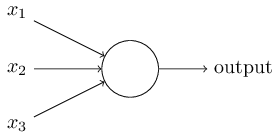
\includegraphics{./img/ch3/3-1.png}
%  
% %\end{figure}

其中\(x_1\),\(x_2\),\(x_3\)为感知机的输入,其输出为:

\[
output = \left\{
\begin{aligned}
0, \quad if \ \ \sum_i w_i x_i \leqslant threshold \\
1, \quad if \ \ \sum_i w_i x_i > threshold
\end{aligned}
\right.
\]

假如把感知机想象成一个加权投票机制,比如 3
位评委给一个歌手打分,打分分别为$ 4 $分、\(1\) 分、$-3$ 分,这 $3$
位评分的权重分别是 \(1、3、2\),则该歌手最终得分为
\(4 \times 1 + 1 \times 3 + (-3) \times 2 = 1\) 。按照比赛规则,选取的
\(threshold\) 为 \(3\),说明只有歌手的综合评分大于$ 3$
时,才可顺利晋级。对照感知机,该选手被淘汰,因为:

\[
\sum_i w_i x_i < threshold=3, output = 0
\]

用 \(-b\) 代替 \(threshold\),输出变为:

\[
output = \left\{
\begin{aligned}
0, \quad if \ \ \boldsymbol{w} \cdot \boldsymbol{x} + b \leqslant 0 \\
1, \quad if \ \ \boldsymbol{w} \cdot \boldsymbol{x} + b > 0
\end{aligned}
\right.
\]

设置合适的 \(\boldsymbol{x}\) 和 \(b\)
,一个简单的感知机单元的与非门表示如下:

% %\begin{figure}
% %\centering
% % 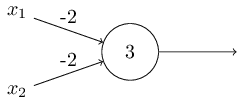
\includegraphics{./img/ch3/3-2.png}
%  
% %\end{figure}

当输入为 \(0\),\(1\) 时,感知机输出为 $ 0 \times (-2) + 1 \times (-2)
+ 3 = 1$。

复杂一些的感知机由简单的感知机单元组合而成:

% %\begin{figure}
% %\centering
% % \includegraphics{./img/ch3/3-3.png}
%  
% %\end{figure}

\textbf{多层感知机}

多层感知机由感知机推广而来,最主要的特点是有多个神经元层,因此也叫深度神经网络。相比于单独的感知机,多层感知机的第
$ i $ 层的每个神经元和第 $ i-1 $ 层的每个神经元都有连接。

% %\begin{figure}
% %\centering
% % \includegraphics{./img/ch3/3.1.1.5.png}
%  
% %\end{figure}

输出层可以不止有$ 1$ 个神经元。隐藏层可以只有$ 1$
层,也可以有多层。输出层为多个神经元的神经网络例如下图所示:

% %\begin{figure}
% %\centering
% % \includegraphics{./img/ch3/3.1.1.6.png}
%  
% %\end{figure}

\subsection{神经网络有哪些常用模型结构?}\label{ux795eux7ecfux7f51ux7edcux6709ux54eaux4e9bux5e38ux7528ux6a21ux578bux7ed3ux6784}

下图包含了大部分常用的模型:

% %\begin{figure}
% %\centering
% % \includegraphics{./img/ch3/3-7.jpg}
%  
% %\end{figure}

\subsection{如何选择深度学习开发平台?}\label{ux5982ux4f55ux9009ux62e9ux6df1ux5ea6ux5b66ux4e60ux5f00ux53d1ux5e73ux53f0}

​ 现有的深度学习开源平台主要有 Caffe, PyTorch, MXNet, CNTK, Theano,
TensorFlow, Keras,
fastai等。那如何选择一个适合自己的平台呢,下面列出一些衡量做参考。

\textbf{参考1:与现有编程平台、技能整合的难易程度}

​ 主要是前期积累的开发经验和资源,比如编程语言,前期数据集存储格式等。

\textbf{参考2: 与相关机器学习、数据处理生态整合的紧密程度}

​
深度学习研究离不开各种数据处理、可视化、统计推断等软件包。考虑建模之前,是否具有方便的数据预处理工具?建模之后,是否具有方便的工具进行可视化、统计推断、数据分析。

\textbf{参考3:对数据量及硬件的要求和支持}

​
深度学习在不同应用场景的数据量是不一样的,这也就导致我们可能需要考虑分布式计算、多GPU计算的问题。例如,对计算机图像处理研究的人员往往需要将图像文件和计算任务分部到多台计算机节点上进行执行。当下每个深度学习平台都在快速发展,每个平台对分布式计算等场景的支持也在不断演进。

\textbf{参考4:深度学习平台的成熟程度}

​
成熟程度的考量是一个比较主观的考量因素,这些因素可包括:社区的活跃程度;是否容易和开发人员进行交流;当前应用的势头。

\textbf{参考5:平台利用是否多样性?}

​
有些平台是专门为深度学习研究和应用进行开发的,有些平台对分布式计算、GPU
等构架都有强大的优化,能否用这些平台/软件做其他事情?比如有些深度学习软件是可以用来求解二次型优化;有些深度学习平台很容易被扩展,被运用在强化学习的应用中。

\subsection{为什么使用深层表示?}\label{ux4e3aux4ec0ux4e48ux4f7fux7528ux6df1ux5c42ux8868ux793a}

\begin{enumerate}
\def\labelenumi{\arabic{enumi}.}
 
\item
  深度神经网络是一种特征递进式的学习算法,浅层的神经元直接从输入数据中学习一些低层次的简单特征,例如边缘、纹理等。而深层的特征则基于已学习到的浅层特征继续学习更高级的特征,从计算机的角度学习深层的语义信息。
\item
  深层的网络隐藏单元数量相对较少,隐藏层数目较多,如果浅层的网络想要达到同样的计算结果则需要指数级增长的单元数量才能达到。
\end{enumerate}

\subsection{为什么深层神经网络难以训练?}\label{ux4e3aux4ec0ux4e48ux6df1ux5c42ux795eux7ecfux7f51ux7edcux96beux4ee5ux8badux7ec3}

\begin{enumerate}
\def\labelenumi{\arabic{enumi}.}
\item
  梯度消失
  梯度消失是指通过隐藏层从后向前看,梯度会变的越来越小,说明前面层的学习会显著慢于后面层的学习,所以学习会卡住,除非梯度变大。

  ​
  梯度消失的原因受到多种因素影响,例如学习率的大小,网络参数的初始化,激活函数的边缘效应等。在深层神经网络中,每一个神经元计算得到的梯度都会传递给前一层,较浅层的神经元接收到的梯度受到之前所有层梯度的影响。如果计算得到的梯度值非常小,随着层数增多,求出的梯度更新信息将会以指数形式衰减,就会发生梯度消失。下图是不同隐含层的学习速率:
\end{enumerate}

% %\begin{figure}
% %\centering
% % \includegraphics{./img/ch3/3-8.png}
%  
% %\end{figure}

\begin{enumerate}
\def\labelenumi{\arabic{enumi}.}
\setcounter{enumi}{1}
\item
  梯度爆炸 在深度网络或循环神经网络(Recurrent Neural Network,
  RNN)等网络结构中,梯度可在网络更新的过程中不断累积,变成非常大的梯度,导致网络权重值的大幅更新,使得网络不稳定;在极端情况下,权重值甚至会溢出,变为\(NaN\)值,再也无法更新。
\item
  权重矩阵的退化导致模型的有效自由度减少。

  ​
  参数空间中学习的退化速度减慢,导致减少了模型的有效维数,网络的可用自由度对学习中梯度范数的贡献不均衡,随着相乘矩阵的数量(即网络深度)的增加,矩阵的乘积变得越来越退化。在有硬饱和边界的非线性网络中(例如
  ReLU
  网络),随着深度增加,退化过程会变得越来越快。Duvenaud等人2014年的论文里展示了关于该退化过程的可视化:
\end{enumerate}

%\begin{figure}
%\centering
% \includegraphics{./img/ch3/3-9.jpg}
 
%\end{figure}

随着深度的增加,输入空间(左上角所示)会在输入空间中的每个点处被扭曲成越来越细的单丝,只有一个与细丝正交的方向影响网络的响应。沿着这个方向,网络实际上对变化变得非常敏感。

\subsection{深度学习和机器学习有什么不同?}\label{ux6df1ux5ea6ux5b66ux4e60ux548cux673aux5668ux5b66ux4e60ux6709ux4ec0ux4e48ux4e0dux540c}

​
\textbf{机器学习}:利用计算机、概率论、统计学等知识,输入数据,让计算机学会新知识。机器学习的过程,就是训练数据去优化目标函数。

​
\textbf{深度学习}:是一种特殊的机器学习,具有强大的能力和灵活性。它通过学习将世界表示为嵌套的层次结构,每个表示都与更简单的特征相关,而抽象的表示则用于计算更抽象的表示。

​ 传统的机器学习需要定义一些手工特征,从而有目的的去提取目标信息,
非常依赖任务的特异性以及设计特征的专家经验。而深度学习可以从大数据中先学习简单的特征,并从其逐渐学习到更为复杂抽象的深层特征,不依赖人工的特征工程,这也是深度学习在大数据时代受欢迎的一大原因。

%\begin{figure}
%\centering
% \includegraphics{./img/ch3/3.1.6.1.png}
 
%\end{figure}

%\begin{figure}
%\centering
% \includegraphics{./img/ch3/3-11.jpg}
 
%\end{figure}

\section{网络操作与计算}\label{ux7f51ux7edcux64cdux4f5cux4e0eux8ba1ux7b97}

\subsection{前向传播与反向传播?}\label{ux524dux5411ux4f20ux64adux4e0eux53cdux5411ux4f20ux64ad}

神经网络的计算主要有两种:前向传播(foward propagation,
FP)作用于每一层的输入,通过逐层计算得到输出结果;反向传播(backward
propagation, BP)作用于网络的输出,通过计算梯度由深到浅更新网络参数。

\textbf{前向传播}

%\begin{figure}
%\centering
% \includegraphics{./img/ch3/3.2.1.1.png}
 
%\end{figure}

假设上一层结点 $ i,j,k,\ldots{} $ 等一些结点与本层的结点 $ w $
有连接,那么结点 $ w $ 的值怎么算呢?就是通过上一层的 $
i,j,k,\ldots{} $
等结点以及对应的连接权值进行加权和运算,最终结果再加上一个偏置项(图中为了简单省略了),最后在通过一个非线性函数(即激活函数),如
\(ReLu\),\(sigmoid\) 等函数,最后得到的结果就是本层结点 $ w $
的输出。

最终不断的通过这种方法一层层的运算,得到输出层结果。

\textbf{反向传播}

%\begin{figure}
%\centering
% \includegraphics{./img/ch3/3.2.1.2.png}
 
%\end{figure}

由于我们前向传播最终得到的结果,以分类为例,最终总是有误差的,那么怎么减少误差呢,当前应用广泛的一个算法就是梯度下降算法,但是求梯度就要求偏导数,下面以图中字母为例讲解一下:

设最终误差为 $ E $且输出层的激活函数为线性激活函数,对于输出那么 $ E
$ 对于输出节点 $ y\_l $ 的偏导数是 $ y\_l - t\_l $,其中 $ t\_l $
是真实值,$ \frac{\partial y_l}{\partial z_l} $
是指上面提到的激活函数,$ z\_l $ 是上面提到的加权和,那么这一层的 $ E
$ 对于 $ z\_l $ 的偏导数为 $ \frac{\partial E}{\partial z_l} =
\frac{\partial E}{\partial y_l} \frac{\partial y_l}{\partial z_l}
$。同理,下一层也是这么计算,只不过 $ \frac{\partial E}{\partial y_k}
$ 计算方法变了,一直反向传播到输入层,最后有 $
\frac{\partial E}{\partial x_i} = \frac{\partial E}{\partial y_j}
\frac{\partial y_j}{\partial z_j} $,且 $
\frac{\partial z_j}{\partial x_i} = w\_i j
$。然后调整这些过程中的权值,再不断进行前向传播和反向传播的过程,最终得到一个比较好的结果。

\subsection{如何计算神经网络的输出?}\label{ux5982ux4f55ux8ba1ux7b97ux795eux7ecfux7f51ux7edcux7684ux8f93ux51fa}

%\begin{figure}
%\centering
% \includegraphics{./img/ch3/3.2.2.1.png}
 
%\end{figure}

如上图,输入层有三个节点,我们将其依次编号为 1、2、3;隐藏层的 4
个节点,编号依次为 4、5、6、7;最后输出层的两个节点编号为
8、9。比如,隐藏层的节点 4,它和输入层的三个节点 1、2、3
之间都有连接,其连接上的权重分别为是 $ w\_\{41\}, w\_\{42\}, w\_\{43\}
$。

为了计算节点 4 的输出值,我们必须先得到其所有上游节点(也就是节点
1、2、3)的输出值。节点 1、2、3
是输入层的节点,所以,他们的输出值就是输入向量本身。按照上图画出的对应关系,可以看到节点
1、2、3 的输出值分别是 $ x\_1, x\_2, x\_3 $。

\[
a_4 = \sigma(w^T \cdot a) = \sigma(w_{41}x_4 + w_{42}x_2 + w_{43}a_3 + w_{4b})
\]

其中 $ w\_\{4b\} $ 是节点 4 的偏置项。

同样,我们可以继续计算出节点 5、6、7 的输出值 $ a\_5, a\_6, a\_7 $。

计算输出层的节点 8 的输出值 $ y\_1 $:

\[
y_1 = \sigma(w^T \cdot a) = \sigma(w_{84}a_4 + w_{85}a_5 + w_{86}a_6 + w_{87}a_7 + w_{8b})
\]

其中 $ w\_\{8b\} $ 是节点 8 的偏置项。

同理,我们还可以计算出 $ y\_2
$。这样输出层所有节点的输出值计算完毕,我们就得到了在输入向量 $ x\_1,
x\_2, x\_3, x\_4 $ 时,神经网络的输出向量 $ y\_1, y\_2 $
。这里我们也看到,输出向量的维度和输出层神经元个数相同。

\subsection{如何计算卷积神经网络输出值?}\label{ux5982ux4f55ux8ba1ux7b97ux5377ux79efux795eux7ecfux7f51ux7edcux8f93ux51faux503c}

假设有一个 5*5 的图像,使用一个 3*3 的 filter 进行卷积,想得到一个 3*3
的 Feature Map,如下所示:

%\begin{figure}
%\centering
% \includegraphics{./img/ch3/3.2.3.1.png}
 
%\end{figure}

$ x\_\{i,j\} $ 表示图像第 $ i $ 行第 $ j $ 列元素。$ w\_\{m,n\}
$ 表示 filter​ 第 $ m $ 行第 $ n $ 列权重。 $ w\_b $ 表示
\(filter\) 的偏置项。 表\(a_i,_j\)示 feature map 第 $ i$ 行第 $ j $
列元素。 \(f\) 表示激活函数,这里以$ ReLU$ 函数为例。

卷积计算公式如下:

\[
a_{i,j} = f(\sum_{m=0}^2 \sum_{n=0}^2 w_{m,n} x_{i+m, j+n} + w_b )
\]

当步长为 \(1\) 时,计算 feature map 元素 $ a\_\{0,0\} $ 如下:

$$ a\_\{0,0\} = f(\sum\emph{\{m=0\}\^{}2 \sum}\{n=0\}\^{}2 w\_\{m,n\}
x\_\{0+m, 0+n\} + w\_b )

= relu(w\_\{0,0\} x\_\{0,0\} + w\_\{0,1\} x\_\{0,1\} + w\_\{0,2\}
x\_\{0,2\} + w\_\{1,0\} x\_\{1,0\} + \textbackslash{}w\_\{1,1\}
x\_\{1,1\} + w\_\{1,2\} x\_\{1,2\} + w\_\{2,0\} x\_\{2,0\} + w\_\{2,1\}
x\_\{2,1\} + w\_\{2,2\} x\_\{2,2\}) \textbackslash{}

= 1 + 0 + 1 + 0 + 1 + 0 + 0 + 0 + 1 \textbackslash{}

= 4 $$

其计算过程图示如下:

%\begin{figure}
%\centering
% \includegraphics{./img/ch3/3.2.3.2.png}
 
%\end{figure}

以此类推,计算出全部的Feature Map。

%\begin{figure}
%\centering
% \includegraphics{./img/ch3/3.2.3.4.png}
 
%\end{figure}

当步幅为 2 时,Feature Map计算如下

%\begin{figure}
%\centering
% \includegraphics{./img/ch3/3.2.3.5.png}
 
%\end{figure}

注:图像大小、步幅和卷积后的Feature
Map大小是有关系的。它们满足下面的关系:

\[
W_2 = (W_1 - F + 2P)/S + 1\\
H_2 = (H_1 - F + 2P)/S + 1
\]

​ 其中 $ W\_2 \(, 是卷积后 Feature Map 的宽度;\) W\_1 $
是卷积前图像的宽度;$ F $ 是 filter 的宽度;$ P $ 是 Zero Padding
数量,Zero Padding 是指在原始图像周围补几圈 \(0\),如果 \(P\) 的值是
\(1\),那么就补 \(1\) 圈 \(0\);\(S\) 是步幅;$ H\_2 $ 卷积后 Feature
Map 的高度;$ H\_1 $ 是卷积前图像的宽度。

​ 举例:假设图像宽度 $ W\_1 = 5 $,filter 宽度 $ F=3 $,Zero Padding
$ P=0 $,步幅 $ S=2 \(,\) Z $ 则

$$ W\_2 = (W\_1 - F + 2P)/S + 1

= (5-3+0)/2 + 1

= 2 $$

​ 说明 Feature Map 宽度是2。同样,我们也可以计算出 Feature Map 高度也是
2。

如果卷积前的图像深度为 $ D $,那么相应的 filter 的深度也必须为 $ D
$。深度大于 1 的卷积计算公式:

\[
a_{i,j} = f(\sum_{d=0}^{D-1} \sum_{m=0}^{F-1} \sum_{n=0}^{F-1} w_{d,m,n} x_{d,i+m,j+n} + w_b)
\]

​ 其中,$ D $ 是深度;$ F $ 是 filter 的大小;$ w\_\{d,m,n\} $
表示 filter 的第 $ d $ 层第 $ m $ 行第 $ n $ 列权重;$
a\_\{d,i,j\} $ 表示 feature map 的第 $ d $ 层第 $ i $ 行第 $ j $
列像素;其它的符号含义前面相同,不再赘述。

​ 每个卷积层可以有多个 filter。每个 filter
和原始图像进行卷积后,都可以得到一个 Feature Map。卷积后 Feature Map
的深度(个数)和卷积层的 filter 个数相同。下面的图示显示了包含两个 filter
的卷积层的计算。\(7*7*3\) 输入,经过两个 \(3*3*3\) filter 的卷积(步幅为
\(2\)),得到了 \(3*3*2\) 的输出。图中的 Zero padding 是
\(1\),也就是在输入元素的周围补了一圈 \(0\)。

%\begin{figure}
%\centering
% \includegraphics{./img/ch3/3.2.3.6.png}
 
%\end{figure}

​
以上就是卷积层的计算方法。这里面体现了局部连接和权值共享:每层神经元只和上一层部分神经元相连(卷积计算规则),且
filter 的权值对于上一层所有神经元都是一样的。对于包含两个 $ 3 * 3 * 3
$ 的 fitler 的卷积层来说,其参数数量仅有 $ (3 * 3 * 3+1) * 2 = 56 $
个,且参数数量与上一层神经元个数无关。与全连接神经网络相比,其参数数量大大减少了。

\subsection{ 如何计算 Pooling层输出值输出值?}\label{ux5982ux4f55ux8ba1ux7b97-pooling-ux5c42ux8f93ux51faux503cux8f93ux51faux503c}

​ Pooling 层主要的作用是下采样,通过去掉 Feature Map
中不重要的样本,进一步减少参数数量。Pooling 的方法很多,最常用的是 Max
Pooling。Max Pooling 实际上就是在 n*n
的样本中取最大值,作为采样后的样本值。下图是 2*2 max pooling:

%\begin{figure}
%\centering
% \includegraphics{./img/ch3/3.2.4.1.png}
 
%\end{figure}

​ 除了 Max Pooing 之外,常用的还有 Average Pooling
------取各样本的平均值。 ​ 对于深度为 $ D $ 的 Feature Map,各层独立做
Pooling,因此 Pooling 后的深度仍然为 $ D $。

\subsection{实例理解反向传播}\label{ux5b9eux4f8bux7406ux89e3ux53cdux5411ux4f20ux64ad}

​ 一个典型的三层神经网络如下所示:

%\begin{figure}
%\centering
% \includegraphics{./img/ch3/3.2.5.1.png}
 
%\end{figure}

​ 其中 Layer $ L\_1 $ 是输入层,Layer $ L\_2 $ 是隐含层,Layer $
L\_3 $ 是输出层。

​ 假设输入数据集为 $ D=\{x\_1, x\_2, \ldots{}, x\_n\} $,输出数据集为
$ y\_1, y\_2, \ldots{}, y\_n $。

​
如果输入和输出是一样,即为自编码模型。如果原始数据经过映射,会得到不同于输入的输出。

假设有如下的网络层:

%\begin{figure}
%\centering
% \includegraphics{./img/ch3/3.2.5.2.png}
 
%\end{figure}

​ 输入层包含神经元 $ i\_1, i\_2 $,偏置 $ b\_1 $;隐含层包含神经元
$ h\_1, h\_2 $,偏置 $ b\_2 $,输出层为 $ o\_1, o\_2 \(,\) w\_i $
为层与层之间连接的权重,激活函数为 \(sigmoid\)
函数。对以上参数取初始值,如下图所示:

%\begin{figure}
%\centering
% \includegraphics{./img/ch3/3.2.5.3.png}
 
%\end{figure}

其中:

\begin{itemize}
 
\item
  输入数据 $ i1=0.05, i2 = 0.10 $
\item
  输出数据 $ o1=0.01, o2=0.99 $;
\item
  初始权重 $ w1=0.15, w2=0.20, w3=0.25,w4=0.30, w5=0.40, w6=0.45,
  w7=0.50, w8=0.55 $
\item
  目标:给出输入数据 $ i1,i2 $ ( \(0.05\)和\(0.10\)  ),使输出尽可能与原始输出 $ o1,o2 $,( \(0.01\)和\(0.99\))接近。
\end{itemize}

\textbf{前向传播}

\begin{enumerate}
\def\labelenumi{\arabic{enumi}.}
 
\item
  输入层 --\textgreater{} 输出层
\end{enumerate}

计算神经元 $ h1 $ 的输入加权和:

$$ net\_\{h1\} = w\_1 * i\_1 + w\_2 * i\_2 + b\_1 * 1\textbackslash{}

net\_\{h1\} = 0.15 * 0.05 + 0.2 * 0.1 + 0.35 * 1 = 0.3775 $$

神经元 $ h1 $ 的输出 $ o1 $ :(此处用到激活函数为 sigmoid 函数):

\[
out_{h1} = \frac{1}{1 + e^{-net_{h1}}} = \frac{1}{1 + e^{-0.3775}} = 0.593269992
\]

同理,可计算出神经元 $ h2 $ 的输出 $ o1 $:

\[
out_{h2} = 0.596884378
\]

\begin{enumerate}
\def\labelenumi{\arabic{enumi}.}
\setcounter{enumi}{1}
 
\item
  隐含层--\textgreater{}输出层:   
\end{enumerate}

计算输出层神经元 $ o1 $ 和 $ o2 $ 的值:

\[
net_{o1} = w_5 * out_{h1} + w_6 * out_{h2} + b_2 * 1
\]

\[
net_{o1} = 0.4 * 0.593269992 + 0.45 * 0.596884378 + 0.6 * 1 = 1.105905967
\]

\[
out_{o1} = \frac{1}{1 + e^{-net_{o1}}} = \frac{1}{1 + e^{1.105905967}} = 0.75136079
\]

这样前向传播的过程就结束了,我们得到输出值为 $ {[}0.75136079 ,
0.772928465{]} $,与实际值 $ {[}0.01 , 0.99{]} $
相差还很远,现在我们对误差进行反向传播,更新权值,重新计算输出。

\textbf{反向传播 }

​ 1.计算总误差

总误差:(这里使用Square Error)

\[
E_{total} = \sum \frac{1}{2}(target - output)^2
\]

但是有两个输出,所以分别计算 $ o1 $ 和 $ o2 $
的误差,总误差为两者之和:

\(E_{o1} = \frac{1}{2}(target_{o1} - out_{o1})^2 = \frac{1}{2}(0.01 - 0.75136507)^2 = 0.274811083\).

\(E_{o2} = 0.023560026\).

\(E_{total} = E_{o1} + E_{o2} = 0.274811083 + 0.023560026 = 0.298371109\).

​ 2.隐含层 --\textgreater{} 输出层的权值更新:

以权重参数 $ w5 $ 为例,如果我们想知道 $ w5 $
对整体误差产生了多少影响,可以用整体误差对 $ w5 $
求偏导求出:(链式法则)

\[
\frac{\partial E_{total}}{\partial w5} = \frac{\partial E_{total}}{\partial out_{o1}} * \frac{\partial out_{o1}}{\partial net_{o1}} * \frac{\partial net_{o1}}{\partial w5}
\]

下面的图可以更直观的看清楚误差是怎样反向传播的:

%\begin{figure}
%\centering
% \includegraphics{./img/ch3/3.2.5.4.png}
 
%\end{figure}

\subsection{ 神经网络更深有什么意义?}
\label{ux795eux7ecfux7f51ux7edcux66f4ux6df1ux6709ux4ec0ux4e48ux610fux4e49}
前提:在一定范围内。

\begin{itemize}
\item
  在神经元数量相同的情况下,深层网络结构具有更大容量,分层组合带来的是指数级的表达空间,能够组合成更多不同类型的子结构,这样可以更容易地学习和表示各种特征。
\item
  隐藏层增加则意味着由激活函数带来的非线性变换的嵌套层数更多,就能构造更复杂的映射关系。
\end{itemize}

\section{ 超参数}\label{ux8d85ux53c2ux6570}

\subsection{什么是超参数?}\label{ux4ec0ux4e48ux662fux8d85ux53c2ux6570}

​ \textbf{超参数} :
在机器学习的上下文中,超参数是在开始学习过程之前设置值的参数,而不是通过训练得到的参数数据。通常情况下,需要对超参数进行优化,给学习机选择一组最优超参数,以提高学习的性能和效果。

​ 超参数通常存在于:

\begin{verbatim}
1.  定义关于模型的更高层次的概念,如复杂性或学习能力。
2.  不能直接从标准模型培训过程中的数据中学习,需要预先定义。
3.  可以通过设置不同的值,训练不同的模型和选择更好的测试值来决定
\end{verbatim}

​ 超参数具体来讲比如算法中的学习率(learning
rate)、梯度下降法迭代的数量(iterations)、隐藏层数目(hidden
layers)、隐藏层单元数目、激活函数( activation
function)都需要根据实际情况来设置,这些数字实际上控制了最后的参数和的值,所以它们被称作超参数。

\subsection{如何寻找超参数的最优值?}\label{ux5982ux4f55ux5bfbux627eux8d85ux53c2ux6570ux7684ux6700ux4f18ux503c}

​
在使用机器学习算法时,总有一些难调的超参数。例如权重衰减大小,高斯核宽度等等。这些参数需要人为设置,设置的值对结果产生较大影响。常见设置超参数的方法有:

\begin{enumerate}
\def\labelenumi{\arabic{enumi}.}
\item
  猜测和检查:根据经验或直觉,选择参数,一直迭代。
\item
  网格搜索:让计算机尝试在一定范围内均匀分布的一组值。
\item
  随机搜索:让计算机随机挑选一组值。
\item
  贝叶斯优化:使用贝叶斯优化超参数,会遇到贝叶斯优化算法本身就需要很多的参数的困难。
\item
  MITIE方法,好初始猜测的前提下进行局部优化。它使用BOBYQA算法,并有一个精心选择的起始点。由于BOBYQA只寻找最近的局部最优解,所以这个方法是否成功很大程度上取决于是否有一个好的起点。在MITIE的情况下,我们知道一个好的起点,但这不是一个普遍的解决方案,因为通常你不会知道好的起点在哪里。从好的方面来说,这种方法非常适合寻找局部最优解。稍后我会再讨论这一点。
\item
  最新提出的LIPO的全局优化方法。这个方法没有参数,而且经验证比随机搜索方法好。
\end{enumerate}

\subsection{超参数搜索一般过程?}\label{ux8d85ux53c2ux6570ux641cux7d22ux4e00ux822cux8fc7ux7a0b}

超参数搜索一般过程: 1. 将数据集划分成训练集、验证集及测试集。 2.
在训练集上根据模型的性能指标对模型参数进行优化。 3.
在验证集上根据模型的性能指标对模型的超参数进行搜索。 4. 步骤 2 和步骤 3
交替迭代,最终确定模型的参数和超参数,在测试集中验证评价模型的优劣。

其中,搜索过程需要搜索算法,一般有:网格搜索、随机搜过、启发式智能搜索、贝叶斯搜索。

\section{ 激活函数}\label{ux6fc0ux6d3bux51fdux6570}

\subsection{为什么需要非线性激活函数?}\label{ux4e3aux4ec0ux4e48ux9700ux8981ux975eux7ebfux6027ux6fc0ux6d3bux51fdux6570}

\textbf{为什么需要激活函数?}

\begin{enumerate}
\def\labelenumi{\arabic{enumi}.}
 
\item
  激活函数对模型学习、理解非常复杂和非线性的函数具有重要作用。
\item
  激活函数可以引入非线性因素。如果不使用激活函数,则输出信号仅是一个简单的线性函数。线性函数一个一级多项式,线性方程的复杂度有限,从数据中学习复杂函数映射的能力很小。没有激活函数,神经网络将无法学习和模拟其他复杂类型的数据,例如图像、视频、音频、语音等。
\item
  激活函数可以把当前特征空间通过一定的线性映射转换到另一个空间,让数据能够更好的被分类。
\end{enumerate}

\textbf{为什么激活函数需要非线性函数?}

\begin{enumerate}
\def\labelenumi{\arabic{enumi}.}
 
\item
  假若网络中全部是线性部件,那么线性的组合还是线性,与单独一个线性分类器无异。这样就做不到用非线性来逼近任意函数。
\item
  使用非线性激活函数
  ,以便使网络更加强大,增加它的能力,使它可以学习复杂的事物,复杂的表单数据,以及表示输入输出之间非线性的复杂的任意函数映射。使用非线性激活函数,能够从输入输出之间生成非线性映射。
\end{enumerate}

\subsection{常见的激活函数及图像}\label{ux5e38ux89c1ux7684ux6fc0ux6d3bux51fdux6570ux53caux56feux50cf}

\begin{enumerate}
\def\labelenumi{\arabic{enumi}.}
 
\item
  sigmoid 激活函数
\end{enumerate}

函数的定义为:$ f(x) = \frac{1}{1 + e^{-x}} $,其值域为 $ (0,1) $。

函数图像如下:

%\begin{figure}
%\centering
% \includegraphics{./img/ch3/3-26.png}
 
%\end{figure}

\begin{enumerate}
\def\labelenumi{\arabic{enumi}.}
\setcounter{enumi}{1}
 
\item
  tanh激活函数
\end{enumerate}

函数的定义为:$ f(x) = tanh(x) = \frac{e^x - e^{-x}}{e^x + e^{-x}}
$,值域为 $ (-1,1) $。

函数图像如下:

%\begin{figure}
%\centering
% \includegraphics{./img/ch3/3-27.png}
 
%\end{figure}

\begin{enumerate}
\def\labelenumi{\arabic{enumi}.}
\setcounter{enumi}{2}
 
\item
  Relu激活函数
\end{enumerate}

函数的定义为:$ f(x) = max(0, x) $ ,值域为 $ {[}0,+∞) $;

函数图像如下:

%\begin{figure}
%\centering
% \includegraphics{./img/ch3/3-28.png}
 
%\end{figure}

\begin{enumerate}
\def\labelenumi{\arabic{enumi}.}
\setcounter{enumi}{3}
 
\item
  Leak Relu 激活函数
\end{enumerate}

函数定义为: $ f(x) = \left\{

\begin{aligned}
   ax, \quad x<0 \\
   x, \quad x>0
   \end{aligned}

\right. $,值域为 $ (-∞,+∞) $。

图像如下($ a = 0.5 $):

%\begin{figure}
%\centering
% \includegraphics{./img/ch3/3-29.png}
 
%\end{figure}

\begin{enumerate}
\def\labelenumi{\arabic{enumi}.}
\setcounter{enumi}{4}
 
\item
  SoftPlus 激活函数
\end{enumerate}

函数的定义为:$ f(x) = ln( 1 + e\^{}x) $,值域为 $ (0,+∞) $。

函数图像如下:

%\begin{figure}
%\centering
% \includegraphics{./img/ch3/3-30.png}
 
%\end{figure}

\begin{enumerate}
\def\labelenumi{\arabic{enumi}.}
\setcounter{enumi}{5}
 
\item
  softmax 函数
\end{enumerate}

函数定义为: $ \sigma(z)\_j = \frac{e^{z_j}}{\sum_{k=1}^K e^{z_k}} $。

Softmax 多用于多分类神经网络输出。

\subsection{3.4.3
常见激活函数的导数计算?}\label{ux5e38ux89c1ux6fc0ux6d3bux51fdux6570ux7684ux5bfcux6570ux8ba1ux7b97}

对常见激活函数,导数计算如下:

\begin{longtable}[]{ llll }
\toprule
\begin{minipage}[b]{0.08\columnwidth}\raggedright\strut
原函数\strut
\end{minipage} & \begin{minipage}[b]{0.22\columnwidth}\raggedright\strut
函数表达式\strut
\end{minipage} & \begin{minipage}[b]{0.30\columnwidth}\raggedright\strut
导数\strut
\end{minipage} & \begin{minipage}[b]{0.30\columnwidth}\raggedright\strut
备注\strut
\end{minipage}\tabularnewline
\midrule
\endhead
\begin{minipage}[t]{0.08\columnwidth}\raggedright\strut
Sigmoid激活函数\strut
\end{minipage} & \begin{minipage}[t]{0.22\columnwidth}\raggedright\strut
\(f(x)=\frac{1}{1+e^{-x}}\)\strut
\end{minipage} & \begin{minipage}[t]{0.30\columnwidth}\raggedright\strut
\(f^{'}(x)=\frac{1}{1+e^{-x}}\left( 1- \frac{1}{1+e^{-x}} \right)=f(x)(1-f(x))\)\strut
\end{minipage} & \begin{minipage}[t]{0.30\columnwidth}\raggedright\strut
当\(x=10\),或\(x=-10​\),\(f^{'}(x) \approx0​\),当\(x=0​\)\(f^{'}(x) =0.25​\)\strut
\end{minipage}\tabularnewline
\begin{minipage}[t]{0.08\columnwidth}\raggedright\strut
Tanh激活函数\strut
\end{minipage} & \begin{minipage}[t]{0.22\columnwidth}\raggedright\strut
\(f(x)=tanh(x)=\frac{e^x-e^{-x}}{e^x+e^{-x}}\)\strut
\end{minipage} & \begin{minipage}[t]{0.30\columnwidth}\raggedright\strut
\(f^{'}(x)=-(tanh(x))^2\)\strut
\end{minipage} & \begin{minipage}[t]{0.30\columnwidth}\raggedright\strut
当\(x=10\),或\(x=-10\),\(f^{'}(x) \approx0\),当\(x=0\)\(f^{`}(x) =1\)\strut
\end{minipage}\tabularnewline
\begin{minipage}[t]{0.08\columnwidth}\raggedright\strut
Relu激活函数\strut
\end{minipage} & \begin{minipage}[t]{0.22\columnwidth}\raggedright\strut
\(f(x)=max(0,x)\)\strut
\end{minipage} & \begin{minipage}[t]{0.30\columnwidth}\raggedright\strut
\(c(u)=\begin{cases} 0,x<0 \\ 1,x>0 \\ undefined,x=0\end{cases}\)\strut
\end{minipage} & \begin{minipage}[t]{0.30\columnwidth}\raggedright\strut
通常\(x=0\)时,给定其导数为1和0\strut
\end{minipage}\tabularnewline
\bottomrule
\end{longtable}

\subsection{激活函数有哪些性质?}\label{ux6fc0ux6d3bux51fdux6570ux6709ux54eaux4e9bux6027ux8d28}

\begin{enumerate}
\def\labelenumi{\arabic{enumi}.}
 
\item
  非线性:
  当激活函数是非线性的,一个两层的神经网络就可以基本上逼近所有的函数。但如果激活函数是恒等激活函数的时候,即
  $ f(x)=x $,就不满足这个性质,而且如果 MLP
  使用的是恒等激活函数,那么其实整个网络跟单层神经网络是等价的;
\item
  可微性: 当优化方法是基于梯度的时候,就体现了该性质;
\item
  单调性: 当激活函数是单调的时候,单层网络能够保证是凸函数;
\item
  $ f(x)≈x $:
  当激活函数满足这个性质的时候,如果参数的初始化是随机的较小值,那么神经网络的训练将会很高效;如果不满足这个性质,那么就需要详细地去设置初始值;
\item
  输出值的范围:
  当激活函数输出值是有限的时候,基于梯度的优化方法会更加稳定,因为特征的表示受有限权值的影响更显著;当激活函数的输出是无限的时候,模型的训练会更加高效,不过在这种情况小,一般需要更小的
  Learning Rate。
\end{enumerate}

\subsection{如何选择激活函数?}\label{ux5982ux4f55ux9009ux62e9ux6fc0ux6d3bux51fdux6570}

​
选择一个适合的激活函数并不容易,需要考虑很多因素,通常的做法是,如果不确定哪一个激活函数效果更好,可以把它们都试试,然后在验证集或者测试集上进行评价。然后看哪一种表现的更好,就去使用它。

以下是常见的选择情况:

\begin{enumerate}
\def\labelenumi{\arabic{enumi}.}
 
\item
  如果输出是 0、1 值(二分类问题),则输出层选择 sigmoid
  函数,然后其它的所有单元都选择 Relu 函数。
\item
  如果在隐藏层上不确定使用哪个激活函数,那么通常会使用 Relu
  激活函数。有时,也会使用 tanh 激活函数,但 Relu
  的一个优点是:当是负值的时候,导数等于 0。
\item
  sigmoid 激活函数:除了输出层是一个二分类问题基本不会用它。
\item
  tanh 激活函数:tanh 是非常优秀的,几乎适合所有场合。
\item
  ReLu 激活函数:最常用的默认函数,如果不确定用哪个激活函数,就使用 ReLu
  或者 Leaky ReLu,再去尝试其他的激活函数。
\item
  如果遇到了一些死的神经元,我们可以使用 Leaky ReLU 函数。
\end{enumerate}

\subsection{ 使用 ReLu激活函数的优点?}\label{ux4f7fux7528-relu-ux6fc0ux6d3bux51fdux6570ux7684ux4f18ux70b9}

\begin{enumerate}
\def\labelenumi{\arabic{enumi}.}
 
\item
  在区间变动很大的情况下,ReLu
  激活函数的导数或者激活函数的斜率都会远大于 0,在程序实现就是一个
  if-else 语句,而 sigmoid 函数需要进行浮点四则运算,在实践中,使用 ReLu
  激活函数神经网络通常会比使用 sigmoid 或者 tanh 激活函数学习的更快。
\item
  sigmoid 和 tanh 函数的导数在正负饱和区的梯度都会接近于
  0,这会造成梯度弥散,而 Relu 和Leaky ReLu 函数大于 0
  部分都为常数,不会产生梯度弥散现象。
\item
  需注意,Relu 进入负半区的时候,梯度为
  0,神经元此时不会训练,产生所谓的稀疏性,而 Leaky ReLu
  不会产生这个问题。
\end{enumerate}

\subsection{3.4.7
什么时候可以用线性激活函数?}\label{ux4ec0ux4e48ux65f6ux5019ux53efux4ee5ux7528ux7ebfux6027ux6fc0ux6d3bux51fdux6570}

\begin{enumerate}
\def\labelenumi{\arabic{enumi}.}
 
\item
  输出层,大多使用线性激活函数。
\item
  在隐含层可能会使用一些线性激活函数。
\item
  一般用到的线性激活函数很少。
\end{enumerate}

\subsection{3.4.8 怎样理解 Relu(\textless{} 0
时)是非线性激活函数?}\label{ux600eux6837ux7406ux89e3-relu-0-ux65f6ux662fux975eux7ebfux6027ux6fc0ux6d3bux51fdux6570}

Relu 激活函数图像如下:

%\begin{figure}
%\centering
% \includegraphics{./img/ch3/3-32.png}
 
%\end{figure}

根据图像可看出具有如下特点:

\begin{enumerate}
\def\labelenumi{\arabic{enumi}.}
\item
  单侧抑制;
\item
  相对宽阔的兴奋边界;
\item
  稀疏激活性;
\end{enumerate}

ReLU 函数从图像上看,是一个分段线性函数,把所有的负值都变为
0,而正值不变,这样就成为单侧抑制。

因为有了这单侧抑制,才使得神经网络中的神经元也具有了稀疏激活性。

\textbf{稀疏激活性}:从信号方面来看,即神经元同时只对输入信号的少部分选择性响应,大量信号被刻意的屏蔽了,这样可以提高学习的精度,更好更快地提取稀疏特征。当
$ x\textless{}0 $ 时,ReLU 硬饱和,而当 $ x\textgreater{}0 $
时,则不存在饱和问题。ReLU 能够在 $ x\textgreater{}0 $
时保持梯度不衰减,从而缓解梯度消失问题。

\subsection{3.4.9 Softmax
定义及作用}\label{softmax-ux5b9aux4e49ux53caux4f5cux7528}

Softmax 是一种形如下式的函数: \[
P(i) = \frac{exp(\theta_i^T x)}{\sum_{k=1}^{K} exp(\theta_i^T x)}
\] ​ 其中,$ \theta\_i $ 和 $ x $ 是列向量,$ \theta\_i\^{}T x $
可能被换成函数关于 $ x $ 的函数 $ f\_i(x) $

​ 通过 softmax 函数,可以使得 $ P(i) $ 的范围在 $ {[}0,1{]} $
之间。在回归和分类问题中,通常 $ \theta $ 是待求参数,通过寻找使得 $
P(i) $ 最大的 $ \theta\_i $ 作为最佳参数。

​ 但是,使得范围在 $ {[}0,1{]} $ 之间的方法有很多,为啥要在前面加上以
$ e $ 的幂函数的形式呢?参考 logistic 函数: \[
P(i) = \frac{1}{1+exp(-\theta_i^T x)}
\] ​ 这个函数的作用就是使得 $ P(i) $ 在负无穷到 0 的区间趋向于 0, 在
0 到正无穷的区间趋向 1,。同样 softmax 函数加入了 $ e $
的幂函数正是为了两极化:正样本的结果将趋近于 1,而负样本的结果趋近于
0。这样为多类别提供了方便(可以把 $ P(i) $
看做是样本属于类别的概率)。可以说,Softmax 函数是 logistic
函数的一种泛化。

​ softmax 函数可以把它的输入,通常被称为 logits 或者 logit
scores,处理成 0 到 1 之间,并且能够把输出归一化到和为 1。这意味着
softmax
函数与分类的概率分布等价。它是一个网络预测多酚类问题的最佳输出激活函数。

\subsection{3.4.10 Softmax
函数如何应用于多分类?}\label{softmax-ux51fdux6570ux5982ux4f55ux5e94ux7528ux4e8eux591aux5206ux7c7b}

​ softmax 用于多分类过程中,它将多个神经元的输出,映射到 $ (0,1) $
区间内,可以看成概率来理解,从而来进行多分类!

​ 假设我们有一个数组,$ V\_i $ 表示 $ V $ 中的第 $ i $
个元素,那么这个元素的 softmax 值就是

\[
S_i = \frac{e^{V_i}}{\sum_j e^{V_j}}
\]

​ 从下图看,神经网络中包含了输入层,然后通过两个特征层处理,最后通过
softmax 分析器就能得到不同条件下的概率,这里需要分成三个类别,最终会得到
$ y=0, y=1, y=2 $ 的概率值。

%\begin{figure}
%\centering
% \includegraphics{./img/ch3/3.4.9.1.png}
 
%\end{figure}

继续看下面的图,三个输入通过 softmax 后得到一个数组 $ {[}0.05 , 0.10 ,
0.85{]} $,这就是 soft 的功能。

%\begin{figure}
%\centering
% \includegraphics{./img/ch3/3.4.9.2.png}
 
%\end{figure}

更形象的映射过程如下图所示:

%\begin{figure}
%\centering
% \includegraphics{./img/ch3/3.4.9.3.png}
\caption{****}
%\end{figure}

​ softmax 直白来说就是将原来输出是 $ 3,1,-3 $ 通过 softmax
函数一作用,就映射成为 $ (0,1) $ 的值,而这些值的累和为 $ 1
$(满足概率的性质),那么我们就可以将它理解成概率,在最后选取输出结点的时候,我们就可以选取概率最大(也就是值对应最大的)结点,作为我们的预测目标!

\subsection{3.4.11
交叉熵代价函数定义及其求导推导}\label{ux4ea4ux53c9ux71b5ux4ee3ux4ef7ux51fdux6570ux5b9aux4e49ux53caux5176ux6c42ux5bfcux63a8ux5bfc}

(\textbf{贡献者:黄钦建-华南理工大学})

​ 神经元的输出就是 a = σ(z),其中\(z=\sum w_{j}i_{j}+b\)是输⼊的带权和。

\(C=-\frac{1}{n}\sum[ylna+(1-y)ln(1-a)]\)

​ 其中 n 是训练数据的总数,求和是在所有的训练输⼊ x 上进⾏的, y
是对应的⽬标输出。

​
表达式是否解决学习缓慢的问题并不明显。实际上,甚⾄将这个定义看做是代价函数也不是显⽽易⻅的!在解决学习缓慢前,我们来看看交叉熵为何能够解释成⼀个代价函数。

​ 将交叉熵看做是代价函数有两点原因。

​ 第⼀,它是⾮负的, C \textgreater{}
0。可以看出:式子中的求和中的所有独⽴的项都是负数的,因为对数函数的定义域是
(0,1),并且求和前⾯有⼀个负号,所以结果是非负。

​ 第⼆,如果对于所有的训练输⼊
x,神经元实际的输出接近⽬标值,那么交叉熵将接近 0。

​ 假设在这个例⼦中, y = 0 ⽽ a ≈
0。这是我们想到得到的结果。我们看到公式中第⼀个项就消去了,因为 y =
0,⽽第⼆项实际上就是 − ln(1 − a) ≈ 0。反之, y = 1 ⽽ a ≈
1。所以在实际输出和⽬标输出之间的差距越⼩,最终的交叉熵的值就越低了。(这里假设输出结果不是0,就是1,实际分类也是这样的)

​ 综上所述,交叉熵是⾮负的,在神经元达到很好的正确率的时候会接近
0。这些其实就是我们想要的代价函数的特性。其实这些特性也是⼆次代价函数具备的。所以,交叉熵就是很好的选择了。但是交叉熵代价函数有⼀个⽐⼆次代价函数更好的特性就是它避免了学习速度下降的问题。为了弄清楚这个情况,我们来算算交叉熵函数关于权重的偏导数。我们将\(a={\varsigma}(z)\)代⼊到
公式中应⽤两次链式法则,得到:

\(\begin{eqnarray}\frac{\partial C}{\partial w_{j}}&=&-\frac{1}{n}\sum \frac{\partial }{\partial w_{j}}[ylna+(1-y)ln(1-a)]\\&=&-\frac{1}{n}\sum \frac{\partial }{\partial a}[ylna+(1-y)ln(1-a)]*\frac{\partial a}{\partial w_{j}}\\&=&-\frac{1}{n}\sum (\frac{y}{a}-\frac{1-y}{1-a})*\frac{\partial a}{\partial w_{j}}\\&=&-\frac{1}{n}\sum (\frac{y}{\varsigma(z)}-\frac{1-y}{1-\varsigma(z)})\frac{\partial \varsigma(z)}{\partial w_{j}}\\&=&-\frac{1}{n}\sum (\frac{y}{\varsigma(z)}-\frac{1-y}{1-\varsigma(z)}){\varsigma}'(z)x_{j}\end{eqnarray}\)

​ 根据\(\varsigma(z)=\frac{1}{1+e^{-z}}\)
的定义,和⼀些运算,我们可以得到
\({\varsigma}'(z)=\varsigma(z)(1-\varsigma(z))\)。化简后可得:

\(\frac{\partial C}{\partial w_{j}}=\frac{1}{n}\sum x_{j}({\varsigma}(z)-y)\)

​
这是⼀个优美的公式。它告诉我们权重学习的速度受到\(\varsigma(z)-y\),也就是输出中的误差的控制。更⼤的误差,更快的学习速度。这是我们直觉上期待的结果。特别地,这个代价函数还避免了像在⼆次代价函数中类似⽅程中\({\varsigma}'(z)\)导致的学习缓慢。当我们使⽤交叉熵的时候,\({\varsigma}'(z)\)被约掉了,所以我们不再需要关⼼它是不是变得很⼩。这种约除就是交叉熵带来的特效。实际上,这也并不是⾮常奇迹的事情。我们在后⾯可以看到,交叉熵其实只是满⾜这种特性的⼀种选择罢了。

​
根据类似的⽅法,我们可以计算出关于偏置的偏导数。我这⾥不再给出详细的过程,你可以轻易验证得到:

\(\frac{\partial C}{\partial b}=\frac{1}{n}\sum ({\varsigma}(z)-y)\)

​ 再⼀次,
这避免了⼆次代价函数中类似\({\varsigma}'(z)\)项导致的学习缓慢。

\subsection{3.4.12
为什么Tanh收敛速度比Sigmoid快?}\label{ux4e3aux4ec0ux4e48tanhux6536ux655bux901fux5ea6ux6bd4sigmoidux5feb}

\textbf{(贡献者:黄钦建-华南理工大学)}

首先看如下两个函数的求导:

\(tanh^{,}(x)=1-tanh(x)^{2}\in (0,1)\)

\(s^{,}(x)=s(x)*(1-s(x))\in (0,\frac{1}{4}]\)

由上面两个公式可知tanh(x)梯度消失的问题比sigmoid轻,所以Tanh收敛速度比Sigmoid快。

3.4.13

\subsection{3.4.12 内聚外斥 - Center
Loss}\label{ux5185ux805aux5916ux65a5---center-loss}

\textbf{(贡献者:李世轩-加州大学伯克利分校)}

在计算机视觉任务中, 由于其简易性, 良好的表现, 与对分类任务的概率性理解,
Cross Entropy Loss (交叉熵代价) + Softmax
组合被广泛应用于以分类任务为代表的任务中. 在此应用下,
我们可将其学习过程进一步理解为:
更相似(同类/同物体)的图像在特征域中拥有``更近的距离'',
相反则''距离更远``. 换而言之,
我们可以进一步理解为其学习了一种低类内距离(Intra-class
Distance)与高类间距离(Inter-class Distance)的特征判别模型. 在此Center
Loss则可以高效的计算出这种具判别性的特征. 不同于传统的Softmax Loss,
Center Loss通过学习``特征中心''从而最小化其类内距离. 其表达形式如下:

\(L_{C} = \frac{1}{2}\sum^{m}_{i=1}||x_{i}-c_{y_{i}}||^{2}_{2}\)

其中\(x_{i}\)表示FCN(全连接层)之前的特征, \(c_{y_{i}}\)表示第$y\_\{i\}
$个类别的特征中心, \(m\)表示mini-batch的大小.
我们很清楚的看到\(L_{C}\)的终极目标为最小化每个特征与其特征中心的方差,
即最小化类内距离. 其迭代公式为:

\(\frac{\partial L_{C}}{\partial x_{i}}=x_{i}-c_{y_{i}}\)

\(\Delta{c_{j}} = \frac{\sum^{m}_{i=1}\delta(y_{i}=j)\cdot(c_{j}-x_{i})}{1+\sum^{m}_{i=1}\delta(y_{i}=j)}\)

其中$ \delta(condition)=\left\{

\begin{array}{rcl}
1       &      & {condition\ is\ True}\\
0     &      & {otherwise}\\ \end{array}

\right.$

结合Softmax, 我们可以搭配二者使用, 适当平衡这两种监督信号.
在Softmax拉开类间距离的同时, 利用Center Loss最小化类内距离. 例如:

\(\begin{eqnarray}L & = & L_{S} + \lambda L_{C} \\ &=& -\sum^{m}_{i=1}log\frac{e^{W_{y}^{T}x_{i}+b_{y_{i}}}}{\sum^{m}_{i=1}e^{W^{T}_{j}x_{i}+b_{j}}} + \frac{\lambda}{2}\sum^{m}_{i=1}||x_{i}-c_{y_{i}}||^{2}_{2}\\ \end{eqnarray}\)

即便如此, Center Loss仍有它的不足之处:
其特征中心为存储在网络模型之外的额外参数, 不能与模型参数一同优化.
这些额外参数将与记录每一步特征变化的自动回归均值估计(autoregressive mean
estimator)进行更迭. 当需要学习的类别数量较大时,
mini-batch可能无力提供足够的样本进行均值估计. 若此Center
Loss将需要平衡两种监督损失来以确定更迭,
其过程需要一个对平衡超参数的搜索过程, 使得其择值消耗昂贵.

\section{3.5 Batch\_Size}\label{batch_size}

\subsection{3.5.1 为什么需要
Batch\_Size?}\label{ux4e3aux4ec0ux4e48ux9700ux8981-batch_size}

Batch的选择,首先决定的是下降的方向。

如果数据集比较小,可采用全数据集的形式,好处是:

\begin{enumerate}
\def\labelenumi{\arabic{enumi}.}
 
\item
  由全数据集确定的方向能够更好地代表样本总体,从而更准确地朝向极值所在的方向。
\item
  由于不同权重的梯度值差别巨大,因此选取一个全局的学习率很困难。 Full
  Batch Learning 可以使用 Rprop 只基于梯度符号并且针对性单独更新各权值。
\end{enumerate}

对于更大的数据集,假如采用全数据集的形式,坏处是: 1.
随着数据集的海量增长和内存限制,一次性载入所有的数据进来变得越来越不可行。
2. 以 Rprop 的方式迭代,会由于各个 Batch
之间的采样差异性,各次梯度修正值相互抵消,无法修正。这才有了后来 RMSProp
的妥协方案。

\subsection{3.5.2 Batch\_Size
值的选择}\label{batch_size-ux503cux7684ux9009ux62e9}

​ 假如每次只训练一个样本,即 Batch\_Size =
1。线性神经元在均方误差代价函数的错误面是一个抛物面,横截面是椭圆。对于多层神经元、非线性网络,在局部依然近似是抛物面。此时,每次修正方向以各自样本的梯度方向修正,横冲直撞各自为政,难以达到收敛。

​ 既然 Batch\_Size 为全数据集或者Batch\_Size =
1都有各自缺点,可不可以选择一个适中的Batch\_Size值呢?

​ 此时,可采用批梯度下降法(Mini-batches
Learning)。因为如果数据集足够充分,那么用一半(甚至少得多)的数据训练算出来的梯度与用全部数据训练出来的梯度是几乎一样的。

\subsection{3.5.3
在合理范围内,增大Batch\_Size有何好处?}\label{ux5728ux5408ux7406ux8303ux56f4ux5185ux589eux5927batch_sizeux6709ux4f55ux597dux5904}

\begin{enumerate}
\def\labelenumi{\arabic{enumi}.}
 
\item
  内存利用率提高了,大矩阵乘法的并行化效率提高。
\item
  跑完一次
  epoch(全数据集)所需的迭代次数减少,对于相同数据量的处理速度进一步加快。
\item
  在一定范围内,一般来说 Batch\_Size
  越大,其确定的下降方向越准,引起训练震荡越小。
\end{enumerate}

\subsection{3.5.4 盲目增大 Batch\_Size
有何坏处?}\label{ux76f2ux76eeux589eux5927-batch_size-ux6709ux4f55ux574fux5904}

\begin{enumerate}
\def\labelenumi{\arabic{enumi}.}
 
\item
  内存利用率提高了,但是内存容量可能撑不住了。
\item
  跑完一次
  epoch(全数据集)所需的迭代次数减少,要想达到相同的精度,其所花费的时间大大增加了,从而对参数的修正也就显得更加缓慢。
\item
  Batch\_Size 增大到一定程度,其确定的下降方向已经基本不再变化。
\end{enumerate}

\subsection{3.5.5 调节 Batch\_Size
对训练效果影响到底如何?}\label{ux8c03ux8282-batch_size-ux5bf9ux8badux7ec3ux6548ux679cux5f71ux54cdux5230ux5e95ux5982ux4f55}

\begin{enumerate}
\def\labelenumi{\arabic{enumi}.}
 
\item
  Batch\_Size 太小,模型表现效果极其糟糕(error飙升)。
\item
  随着 Batch\_Size 增大,处理相同数据量的速度越快。
\item
  随着 Batch\_Size 增大,达到相同精度所需要的 epoch 数量越来越多。
\item
  由于上述两种因素的矛盾, Batch\_Size
  增大到某个时候,达到时间上的最优。
\item
  由于最终收敛精度会陷入不同的局部极值,因此 Batch\_Size
  增大到某些时候,达到最终收敛精度上的最优。
\end{enumerate}

\section{3.6 归一化}\label{ux5f52ux4e00ux5316}

\subsection{3.6.1 归一化含义?}\label{ux5f52ux4e00ux5316ux542bux4e49}

\begin{enumerate}
\def\labelenumi{\arabic{enumi}.}
\item
  归纳统一样本的统计分布性。归一化在 $ 0-1$
  之间是统计的概率分布,归一化在$ -1--+1$ 之间是统计的坐标分布。
\item
  无论是为了建模还是为了计算,首先基本度量单位要同一,神经网络是以样本在事件中的统计分别几率来进行训练(概率计算)和预测,且
  sigmoid 函数的取值是 0 到 1
  之间的,网络最后一个节点的输出也是如此,所以经常要对样本的输出归一化处理。
\item
  归一化是统一在 $ 0-1 $
  之间的统计概率分布,当所有样本的输入信号都为正值时,与第一隐含层神经元相连的权值只能同时增加或减小,从而导致学习速度很慢。
\item
  另外在数据中常存在奇异样本数据,奇异样本数据存在所引起的网络训练时间增加,并可能引起网络无法收敛。为了避免出现这种情况及后面数据处理的方便,加快网络学习速度,可以对输入信号进行归一化,使得所有样本的输入信号其均值接近于
  0 或与其均方差相比很小。
\end{enumerate}

\subsection{3.6.2
为什么要归一化?}\label{ux4e3aux4ec0ux4e48ux8981ux5f52ux4e00ux5316}

\begin{enumerate}
\def\labelenumi{\arabic{enumi}.}
 
\item
  为了后面数据处理的方便,归一化的确可以避免一些不必要的数值问题。
\item
  为了程序运行时收敛加快。
\item
  同一量纲。样本数据的评价标准不一样,需要对其量纲化,统一评价标准。这算是应用层面的需求。
\item
  避免神经元饱和。啥意思?就是当神经元的激活在接近 0 或者 1
  时会饱和,在这些区域,梯度几乎为
  0,这样,在反向传播过程中,局部梯度就会接近
  0,这会有效地``杀死''梯度。
\item
  保证输出数据中数值小的不被吞食。
\end{enumerate}

\subsection{3.6.3
为什么归一化能提高求解最优解速度?}\label{ux4e3aux4ec0ux4e48ux5f52ux4e00ux5316ux80fdux63d0ux9ad8ux6c42ux89e3ux6700ux4f18ux89e3ux901fux5ea6}

%\begin{figure}
%\centering
% \includegraphics{./img/ch3/3.6.3.1.png}
 
%\end{figure}

​
上图是代表数据是否均一化的最优解寻解过程(圆圈可以理解为等高线)。左图表示未经归一化操作的寻解过程,右图表示经过归一化后的寻解过程。

​
当使用梯度下降法寻求最优解时,很有可能走``之字型''路线(垂直等高线走),从而导致需要迭代很多次才能收敛;而右图对两个原始特征进行了归一化,其对应的等高线显得很圆,在梯度下降进行求解时能较快的收敛。

​
因此如果机器学习模型使用梯度下降法求最优解时,归一化往往非常有必要,否则很难收敛甚至不能收敛。

\subsection{3.6.4 3D
图解未归一化}\label{d-ux56feux89e3ux672aux5f52ux4e00ux5316}

例子:

​ 假设 $ w1 $ 的范围在 $ {[}-10, 10{]} $,而 $ w2 $ 的范围在 $
{[}-100, 100{]} $,梯度每次都前进 1 单位,那么在 $ w1 $
方向上每次相当于前进了 $ 1/20 $,而在 $ w2 $ 上只相当于 $ 1/200
$!某种意义上来说,在 $ w2 $ 上前进的步长更小一些,而 $ w1 $
在搜索过程中会比 $ w2 $ ``走''得更快。

​ 这样会导致,在搜索过程中更偏向于 $ w1 $
的方向。走出了``L''形状,或者成为``之''字形。

%\begin{figure}
%\centering
% \includegraphics{./img/ch3/3-37.png}
 
%\end{figure}

\subsection{3.6.5
归一化有哪些类型?}\label{ux5f52ux4e00ux5316ux6709ux54eaux4e9bux7c7bux578b}

\begin{enumerate}
\def\labelenumi{\arabic{enumi}.}
 
\item
  线性归一化
\end{enumerate}

\[
x^{\prime} = \frac{x-min(x)}{max(x) - min(x)}
\]

​ 适用范围:比较适用在数值比较集中的情况。

​ 缺点:如果 max 和 min
不稳定,很容易使得归一化结果不稳定,使得后续使用效果也不稳定。

\begin{enumerate}
\def\labelenumi{\arabic{enumi}.}
\setcounter{enumi}{1}
 
\item
  标准差标准化
\end{enumerate}

\[
x^{\prime} = \frac{x-\mu}{\sigma}
\]

​ 含义:经过处理的数据符合标准正态分布,即均值为 0,标准差为 1 其中 $
\mu $ 为所有样本数据的均值,$ \sigma $ 为所有样本数据的标准差。

\begin{enumerate}
\def\labelenumi{\arabic{enumi}.}
\setcounter{enumi}{2}
 
\item
  非线性归一化
\end{enumerate}

适用范围:经常用在数据分化比较大的场景,有些数值很大,有些很小。通过一些数学函数,将原始值进行映射。该方法包括
$ log $、指数,正切等。

\subsection{3.6.6
局部响应归一化作用}\label{ux5c40ux90e8ux54cdux5e94ux5f52ux4e00ux5316ux4f5cux7528}

​ LRN 是一种提高深度学习准确度的技术方法。LRN
一般是在激活、池化函数后的一种方法。

​ 在 ALexNet 中,提出了 LRN
层,对局部神经元的活动创建竞争机制,使其中响应比较大对值变得相对更大,并抑制其他反馈较小的神经元,增强了模型的泛化能力。

\subsection{3.6.7
理解局部响应归一化}\label{ux7406ux89e3ux5c40ux90e8ux54cdux5e94ux5f52ux4e00ux5316}

​
局部响应归一化原理是仿造生物学上活跃的神经元对相邻神经元的抑制现象(侧抑制),其公式如下:

\[
b_{x,y}^i = a_{x,y}^i / (k + \alpha \sum_{j=max(0, i-n/2)}^{min(N-1, i+n/2)}(a_{x,y}^j)^2 )^\beta
\]

其中, 1) $ a
$:表示卷积层(包括卷积操作和池化操作)后的输出结果,是一个四维数组{[}batch,height,width,channel{]}。

\begin{itemize}
 
\item
  batch:批次数(每一批为一张图片)。
\item
  height:图片高度。
\item
  width:图片宽度。
\item
  channel:通道数。可以理解成一批图片中的某一个图片经过卷积操作后输出的神经元个数,或理解为处理后的图片深度。
\end{itemize}

\begin{enumerate}
\def\labelenumi{\arabic{enumi})}
\setcounter{enumi}{1}
\item
  $ a\_\{x,y\}\^{}i $ 表示在这个输出结构中的一个位置 $ {[}a,b,c,d{]}
  $,可以理解成在某一张图中的某一个通道下的某个高度和某个宽度位置的点,即第
  $ a $ 张图的第 $ d $ 个通道下的高度为b宽度为c的点。
\item
  $ N $:论文公式中的 $ N $ 表示通道数 (channel)。
\item
  $ a \(,\) n/2 $, $ k $ 分别表示函数中的
  input,depth\_radius,bias。参数 $ k, n, \alpha, \beta $
  都是超参数,一般设置 $ k=2, n=5, \alpha=1*e-4, \beta=0.75 $
\item
  $ \sum \(:\) \sum $
  叠加的方向是沿着通道方向的,即每个点值的平方和是沿着 $ a $ 中的第 3
  维 channel 方向的,也就是一个点同方向的前面 $ n/2 $ 个通道(最小为第
  $ 0 $ 个通道)和后 $ n/2 $ 个通道(最大为第 $ d-1 $
  个通道)的点的平方和(共 $ n+1 $ 个点)。而函数的英文注解中也说明了把
  input 当成是 $ d $ 个 3 维的矩阵,说白了就是把 input 的通道数当作 3
  维矩阵的个数,叠加的方向也是在通道方向。
\end{enumerate}

简单的示意图如下:

%\begin{figure}
%\centering
% \includegraphics{./img/ch3/3.6.7.1.png}
 
%\end{figure}

\subsection{3.6.8 什么是批归一化(Batch
Normalization)}\label{ux4ec0ux4e48ux662fux6279ux5f52ux4e00ux5316batch-normalization}

​
以前在神经网络训练中,只是对输入层数据进行归一化处理,却没有在中间层进行归一化处理。要知道,虽然我们对输入数据进行了归一化处理,但是输入数据经过
$ \sigma(WX+b) $
这样的矩阵乘法以及非线性运算之后,其数据分布很可能被改变,而随着深度网络的多层运算之后,数据分布的变化将越来越大。如果我们能在网络的中间也进行归一化处理,是否对网络的训练起到改进作用呢?答案是肯定的。

​
这种在神经网络中间层也进行归一化处理,使训练效果更好的方法,就是批归一化Batch
Normalization(BN)。

\subsection{3.6.9
批归一化(BN)算法的优点}\label{ux6279ux5f52ux4e00ux5316bnux7b97ux6cd5ux7684ux4f18ux70b9}

下面我们来说一下BN算法的优点: 1.
减少了人为选择参数。在某些情况下可以取消 dropout 和 L2
正则项参数,或者采取更小的 L2 正则项约束参数; 2.
减少了对学习率的要求。现在我们可以使用初始很大的学习率或者选择了较小的学习率,算法也能够快速训练收敛;
3. 可以不再使用局部响应归一化。BN 本身就是归一化网络(局部响应归一化在
AlexNet 网络中存在) 4.
破坏原来的数据分布,一定程度上缓解过拟合(防止每批训练中某一个样本经常被挑选到,文献说这个可以提高
1\% 的精度)。 5. 减少梯度消失,加快收敛速度,提高训练精度。

\subsection{3.6.10
批归一化(BN)算法流程}\label{ux6279ux5f52ux4e00ux5316bnux7b97ux6cd5ux6d41ux7a0b}

下面给出 BN 算法在训练时的过程

输入:上一层输出结果 $ X = \{x\_1, x\_2, \ldots{}, x\_m\} $,学习参数
$ \gamma, \beta $

算法流程:

\begin{enumerate}
\def\labelenumi{\arabic{enumi}.}
 
\item
  计算上一层输出数据的均值
\end{enumerate}

\[
\mu_{\beta} = \frac{1}{m} \sum_{i=1}^m(x_i)
\]

其中,$ m $ 是此次训练样本 batch 的大小。

\begin{enumerate}
\def\labelenumi{\arabic{enumi}.}
\setcounter{enumi}{1}
 
\item
  计算上一层输出数据的标准差
\end{enumerate}

\[
\sigma_{\beta}^2 = \frac{1}{m} \sum_{i=1}^m (x_i - \mu_{\beta})^2
\]

\begin{enumerate}
\def\labelenumi{\arabic{enumi}.}
\setcounter{enumi}{2}
 
\item
  归一化处理,得到
\end{enumerate}

\[
\hat x_i = \frac{x_i + \mu_{\beta}}{\sqrt{\sigma_{\beta}^2} + \epsilon}
\]

其中 $ \epsilon $ 是为了避免分母为 0 而加进去的接近于 0 的很小值

\begin{enumerate}
\def\labelenumi{\arabic{enumi}.}
\setcounter{enumi}{3}
 
\item
  重构,对经过上面归一化处理得到的数据进行重构,得到
\end{enumerate}

\[
y_i = \gamma \hat x_i + \beta
\]

其中,$ \gamma, \beta $ 为可学习参数。

注:上述是 BN
训练时的过程,但是当在投入使用时,往往只是输入一个样本,没有所谓的均值
$ \mu\emph{\{\beta\} $ 和标准差 $ \sigma}\{\beta\}\^{}2
$。此时,均值 $ \mu\emph{\{\beta\} $ 是计算所有 batch $
\mu}\{\beta\} $ 值的平均值得到,标准差 $ \sigma\emph{\{\beta\}\^{}2 $
采用每个batch $ \sigma}\{\beta\}\^{}2 $ 的无偏估计得到。

\subsection{3.6.11
批归一化和群组归一化比较}\label{ux6279ux5f52ux4e00ux5316ux548cux7fa4ux7ec4ux5f52ux4e00ux5316ux6bd4ux8f83}

\begin{longtable}[]{ ll }
\toprule
\begin{minipage}[b]{0.41\columnwidth}\raggedright\strut
名称\strut
\end{minipage} & \begin{minipage}[b]{0.53\columnwidth}\raggedright\strut
特点\strut
\end{minipage}\tabularnewline
\midrule
\endhead
\begin{minipage}[t]{0.41\columnwidth}\raggedright\strut
批量归一化(Batch Normalization,以下简称 BN)\strut
\end{minipage} & \begin{minipage}[t]{0.53\columnwidth}\raggedright\strut
可让各种网络并行训练。但是,批量维度进行归一化会带来一些问题------批量统计估算不准确导致批量变小时,BN
的误差会迅速增加。在训练大型网络和将特征转移到计算机视觉任务中(包括检测、分割和视频),内存消耗限制了只能使用小批量的
BN。\strut
\end{minipage}\tabularnewline
\begin{minipage}[t]{0.41\columnwidth}\raggedright\strut
群组归一化 Group Normalization (简称 GN)\strut
\end{minipage} & \begin{minipage}[t]{0.53\columnwidth}\raggedright\strut
GN 将通道分成组,并在每组内计算归一化的均值和方差。GN
的计算与批量大小无关,并且其准确度在各种批量大小下都很稳定。\strut
\end{minipage}\tabularnewline
\begin{minipage}[t]{0.41\columnwidth}\raggedright\strut
比较\strut
\end{minipage} & \begin{minipage}[t]{0.53\columnwidth}\raggedright\strut
在 ImageNet 上训练的 ResNet-50上,GN 使用批量大小为 2 时的错误率比 BN
的错误率低 10.6% ;当使用典型的批量时,GN 与 BN
相当,并且优于其他标归一化变体。而且,GN
可以自然地从预训练迁移到微调。在进行 COCO 中的目标检测和分割以及
Kinetics 中的视频分类比赛中,GN 可以胜过其竞争对手,表明 GN
可以在各种任务中有效地取代强大的 BN。\strut
\end{minipage}\tabularnewline
\bottomrule
\end{longtable}

\subsection{3.6.12 Weight Normalization和Batch
Normalization比较}\label{weight-normalizationux548cbatch-normalizationux6bd4ux8f83}

​ Weight Normalization 和 Batch Normalization
都属于参数重写(Reparameterization)的方法,只是采用的方式不同。

​ Weight Normalization 是对网络权值$ W $ 进行
normalization,因此也称为 Weight Normalization;

​ Batch Normalization 是对网络某一层输入数据进行 normalization。

​ Weight Normalization相比Batch Normalization有以下三点优势:

\begin{enumerate}
\def\labelenumi{\arabic{enumi}.}
\item
  Weight Normalization
  通过重写深度学习网络的权重W的方式来加速深度学习网络参数收敛,没有引入
  minbatch 的依赖,适用于 RNN(LSTM)网络(Batch Normalization
  不能直接用于RNN,进行 normalization 操作,原因在于:1) RNN 处理的
  Sequence 是变长的;2) RNN 是基于 time step 计算,如果直接使用 Batch
  Normalization 处理,需要保存每个 time step 下,mini btach
  的均值和方差,效率低且占内存)。
\item
  Batch Normalization 基于一个 mini batch
  的数据计算均值和方差,而不是基于整个 Training set
  来做,相当于进行梯度计算式引入噪声。因此,Batch Normalization
  不适用于对噪声敏感的强化学习、生成模型(Generative
  model:GAN,VAE)使用。相反,Weight Normalization 对通过标量 $ g $
  和向量 $ v $ 对权重 $ W $ 进行重写,重写向量 $ v $
  是固定的,因此,基于 Weight Normalization 的 Normalization 可以看做比
  Batch Normalization 引入更少的噪声。
\item
  不需要额外的存储空间来保存 mini batch 的均值和方差,同时实现 Weight
  Normalization
  时,对深度学习网络进行正向信号传播和反向梯度计算带来的额外计算开销也很小。因此,要比采用
  Batch Normalization 进行 normalization 操作时,速度快。 但是 Weight
  Normalization 不具备 Batch Normalization 把网络每一层的输出 Y
  固定在一个变化范围的作用。因此,采用 Weight Normalization 进行
  Normalization 时需要特别注意参数初始值的选择。
\end{enumerate}

\subsection{3.6.13 Batch
Normalization在什么时候用比较合适?}\label{batch-normalizationux5728ux4ec0ux4e48ux65f6ux5019ux7528ux6bd4ux8f83ux5408ux9002}

\textbf{(贡献者:黄钦建-华南理工大学)}

​
在CNN中,BN应作用在非线性映射前。在神经网络训练时遇到收敛速度很慢,或梯度爆炸等无法训练的状况时可以尝试BN来解决。另外,在一般使用情况下也可以加入BN来加快训练速度,提高模型精度。

​
BN比较适用的场景是:每个mini-batch比较大,数据分布比较接近。在进行训练之前,要做好充分的shuffle,否则效果会差很多。另外,由于BN需要在运行过程中统计每个mini-batch的一阶统计量和二阶统计量,因此不适用于动态的网络结构和RNN网络。

\section{3.7 预训练与微调(fine
tuning)}\label{ux9884ux8badux7ec3ux4e0eux5faeux8c03fine-tuning}

\subsection{3.7.1
为什么无监督预训练可以帮助深度学习?}\label{ux4e3aux4ec0ux4e48ux65e0ux76d1ux7763ux9884ux8badux7ec3ux53efux4ee5ux5e2eux52a9ux6df1ux5ea6ux5b66ux4e60}

深度网络存在问题:

\begin{enumerate}
\def\labelenumi{\arabic{enumi}.}
\item
  网络越深,需要的训练样本数越多。若用监督则需大量标注样本,不然小规模样本容易造成过拟合。深层网络特征比较多,会出现的多特征问题主要有多样本问题、规则化问题、特征选择问题。
\item
  多层神经网络参数优化是个高阶非凸优化问题,经常得到收敛较差的局部解;
\item
  梯度扩散问题,BP算法计算出的梯度随着深度向前而显著下降,导致前面网络参数贡献很小,更新速度慢。
\end{enumerate}

\textbf{解决方法:}

​ 逐层贪婪训练,无监督预训练(unsupervised
pre-training)即训练网络的第一个隐藏层,再训练第二个\ldots{}最后用这些训练好的网络参数值作为整体网络参数的初始值。

经过预训练最终能得到比较好的局部最优解。

\subsection{3.7.2 什么是模型微调fine
tuning}\label{ux4ec0ux4e48ux662fux6a21ux578bux5faeux8c03fine-tuning}

​
用别人的参数、修改后的网络和自己的数据进行训练,使得参数适应自己的数据,这样一个过程,通常称之为微调(fine
tuning).

\textbf{模型的微调举例说明:}

​ 我们知道,CNN 在图像识别这一领域取得了巨大的进步。如果想将 CNN
应用到我们自己的数据集上,这时通常就会面临一个问题:通常我们的 dataset
都不会特别大,一般不会超过 1
万张,甚至更少,每一类图片只有几十或者十几张。这时候,直接应用这些数据训练一个网络的想法就不可行了,因为深度学习成功的一个关键性因素就是大量带标签数据组成的训练集。如果只利用手头上这点数据,即使我们利用非常好的网络结构,也达不到很高的
performance。这时候,fine-tuning
的思想就可以很好解决我们的问题:我们通过对 ImageNet
上训练出来的模型(如CaffeNet,VGGNet,ResNet)
进行微调,然后应用到我们自己的数据集上。

\subsection{3.7.3
微调时候网络参数是否更新?}\label{ux5faeux8c03ux65f6ux5019ux7f51ux7edcux53c2ux6570ux662fux5426ux66f4ux65b0}

答案:会更新。

\begin{enumerate}
\def\labelenumi{\arabic{enumi}.}
 
\item
  finetune 的过程相当于继续训练,跟直接训练的区别是初始化的时候。
\item
  直接训练是按照网络定义指定的方式初始化。
\item
  finetune是用你已经有的参数文件来初始化。
\end{enumerate}

\subsection{3.7.4 fine-tuning
模型的三种状态}\label{fine-tuning-ux6a21ux578bux7684ux4e09ux79cdux72b6ux6001}

\begin{enumerate}
\def\labelenumi{\arabic{enumi}.}
\item
  状态一:只预测,不训练。
  特点:相对快、简单,针对那些已经训练好,现在要实际对未知数据进行标注的项目,非常高效;
\item
  状态二:训练,但只训练最后分类层。
  特点:fine-tuning的模型最终的分类以及符合要求,现在只是在他们的基础上进行类别降维。
\item
  状态三:完全训练,分类层+之前卷积层都训练
  特点:跟状态二的差异很小,当然状态三比较耗时和需要训练GPU资源,不过非常适合fine-tuning到自己想要的模型里面,预测精度相比状态二也提高不少。
\end{enumerate}

\section{3.8
权重偏差初始化}\label{ux6743ux91cdux504fux5deeux521dux59cbux5316}

\subsection{3.8.1 全都初始化为
0}\label{ux5168ux90fdux521dux59cbux5316ux4e3a-0}

\textbf{偏差初始化陷阱}: 都初始化为 0。

\textbf{产生陷阱原因}:因为并不知道在训练神经网络中每一个权重最后的值,但是如果进行了恰当的数据归一化后,我们可以有理由认为有一半的权重是正的,另一半是负的。令所有权重都初始化为
0,如果神经网络计算出来的输出值是一样的,神经网络在进行反向传播算法计算出来的梯度值也一样,并且参数更新值也一样。更一般地说,如果权重初始化为同一个值,网络就是对称的。

\textbf{形象化理解}:在神经网络中考虑梯度下降的时候,设想你在爬山,但身处直线形的山谷中,两边是对称的山峰。由于对称性,你所在之处的梯度只能沿着山谷的方向,不会指向山峰;你走了一步之后,情况依然不变。结果就是你只能收敛到山谷中的一个极大值,而走不到山峰上去。

\subsection{3.8.2
全都初始化为同样的值}\label{ux5168ux90fdux521dux59cbux5316ux4e3aux540cux6837ux7684ux503c}

​ 偏差初始化陷阱: 都初始化为一样的值。 ​ 以一个三层网络为例:
首先看下结构

%\begin{figure}
%\centering
% \includegraphics{./img/ch3/3.8.2.1.png}
 
%\end{figure}

它的表达式为:

\[
a_1^{(2)} = f(W_{11}^{(1)} x_1 + W_{12}^{(1)} x_2 + W_{13}^{(1)} x_3 + b_1^{(1)})
\]

\[
a_2^{(2)} = f(W_{21}^{(1)} x_1 + W_{22}^{(1)} x_2 + W_{23}^{(1)} x_3 + b_2^{(1)})
\]

\[
a_3^{(2)} = f(W_{31}^{(1)} x_1 + W_{32}^{(1)} x_2 + W_{33}^{(1)} x_3 + b_3^{(1)})
\]

\[
h_{W,b}(x) = a_1^{(3)} = f(W_{11}^{(2)} a_1^{(2)} + W_{12}^{(2)} a_2^{(2)} + W_{13}^{(2)} a_3^{(2)} + b_1^{(2)})
\]

\[
xa_1^{(2)} = f(W_{11}^{(1)} x_1 + W_{12}^{(1)} x_2 + W_{13}^{(1)} x_3 + b_1^{(1)})a_2^{(2)} = f(W_{21}^{(1)} x_1 + W_{22}^{(1)} x_2 + W_{23}^{(1)} x_3 + 
\]

如果每个权重都一样,那么在多层网络中,从第二层开始,每一层的输入值都是相同的了也就是$
a1=a2=a3=\ldots{}. $,既然都一样,就相当于一个输入了,为啥呢??

如果是反向传递算法(如果这里不明白请看上面的连接),其中的偏置项和权重项的迭代的偏导数计算公式如下

$$ \frac{\partial}{\partial W_{ij}^{(l)}} J(W,b;x,y) = a\_j\^{}\{(l)\}
\delta\_i\^{}\{(l+1)\}

\frac{\partial}{\partial b_{i}^{(l)}} J(W,b;x,y) =
\delta\_i\^{}\{(l+1)\} $$

$ \delta $ 的计算公式

\[
\delta_i^{(l)} = (\sum_{j=1}^{s_{t+1}} W_{ji}^{(l)} \delta_j^{(l+1)} ) f^{\prime}(z_i^{(l)})
\]

如果用的是 sigmoid 函数

\[
f^{\prime}(z_i^{(l)}) = a_i^{(l)}(1-a_i^{(l)})
\]

把后两个公式代入,可以看出所得到的梯度下降法的偏导相同,不停的迭代,不停的相同,不停的迭代,不停的相同\ldots{}\ldots{},最后就得到了相同的值(权重和截距)。

\subsection{3.8.3
初始化为小的随机数}\label{ux521dux59cbux5316ux4e3aux5c0fux7684ux968fux673aux6570}

​
将权重初始化为很小的数字是一个普遍的打破网络对称性的解决办法。这个想法是,神经元在一开始都是随机的、独一无二的,所以它们会计算出不同的更新,并将自己整合到整个网络的各个部分。一个权重矩阵的实现可能看起来像
$ W=0.01∗np.random.randn(D,H) $,其中 randn 是从均值为 0
的单位标准高斯分布进行取样。通过这个公式(函数),每个神经元的权重向量初始化为一个从多维高斯分布取样的随机向量,所以神经元在输入空间中指向随机的方向(so
the neurons point in random direction in the input space).
应该是指输入空间对于随机方向有影响)。其实也可以从均匀分布中来随机选取小数,但是在实际操作中看起来似乎对最后的表现并没有太大的影响。

​
备注:并不是数字越小就会表现的越好。比如,如果一个神经网络层的权重非常小,那么在反向传播算法就会计算出很小的梯度(因为梯度
gradient
是与权重成正比的)。在网络不断的反向传播过程中将极大地减少``梯度信号'',并可能成为深层网络的一个需要注意的问题。

\subsection{\texorpdfstring{3.8.4 用 $ 1/\sqrt n $
校准方差}{3.8.4 用 $ 1/n $ 校准方差}}\label{ux7528-1n-ux6821ux51c6ux65b9ux5dee}

​
上述建议的一个问题是,随机初始化神经元的输出的分布有一个随输入量增加而变化的方差。结果证明,我们可以通过将其权重向量按其输入的平方根(即输入的数量)进行缩放,从而将每个神经元的输出的方差标准化到
1。也就是说推荐的启发式方法 (heuristic)
是将每个神经元的权重向量按下面的方法进行初始化: $
w=np.random.randn(n)/\sqrt n $,其中 n
表示输入的数量。这保证了网络中所有的神经元最初的输出分布大致相同,并在经验上提高了收敛速度。

\subsection{3.8.5 稀疏初始化(Sparse
Initialazation)}\label{ux7a00ux758fux521dux59cbux5316sparse-initialazation}

​
另一种解决未校准方差问题的方法是把所有的权重矩阵都设为零,但是为了打破对称性,每个神经元都是随机连接地(从如上面所介绍的一个小的高斯分布中抽取权重)到它下面的一个固定数量的神经元。一个典型的神经元连接的数目可能是小到
10 个。

\subsection{3.8.6 初始化偏差}\label{ux521dux59cbux5316ux504fux5dee}

​
将偏差初始化为零是可能的,也是很常见的,因为非对称性破坏是由权重的小随机数导致的。因为
ReLU 具有非线性特点,所以有些人喜欢使用将所有的偏差设定为小的常数值如
0.01,因为这样可以确保所有的 ReLU
单元在最开始就激活触发(fire)并因此能够获得和传播一些梯度值。然而,这是否能够提供持续的改善还不太清楚(实际上一些结果表明这样做反而使得性能更加糟糕),所以更通常的做法是简单地将偏差初始化为
0.

\section{3.9 学习率}\label{ux5b66ux4e60ux7387}

\subsection{3.9.1
学习率的作用}\label{ux5b66ux4e60ux7387ux7684ux4f5cux7528}

​
在机器学习中,监督式学习通过定义一个模型,并根据训练集上的数据估计最优参数。梯度下降法是一个广泛被用来最小化模型误差的参数优化算法。梯度下降法通过多次迭代,并在每一步中最小化成本函数(cost
来估计模型的参数。学习率 (learning
rate),在迭代过程中会控制模型的学习进度。

​
在梯度下降法中,都是给定的统一的学习率,整个优化过程中都以确定的步长进行更新,
在迭代优化的前期中,学习率较大,则前进的步长就会较长,这时便能以较快的速度进行梯度下降,而在迭代优化的后期,逐步减小学习率的值,减小步长,这样将有助于算法的收敛,更容易接近最优解。故而如何对学习率的更新成为了研究者的关注点。
​
在模型优化中,常用到的几种学习率衰减方法有:分段常数衰减、多项式衰减、指数衰减、自然指数衰减、余弦衰减、线性余弦衰减、噪声线性余弦衰减

\subsection{学习率衰减常用参数有哪些}\label{ux5b66ux4e60ux7387ux8870ux51cfux5e38ux7528ux53c2ux6570ux6709ux54eaux4e9b}

\begin{longtable}[]{ ll }
\toprule
参数名称 & 参数说明\tabularnewline
\midrule
\endhead
learning\_rate & 初始学习率\tabularnewline
global\_step &
用于衰减计算的全局步数,非负,用于逐步计算衰减指数\tabularnewline
decay\_steps & 衰减步数,必须是正值,决定衰减周期\tabularnewline
decay\_rate & 衰减率\tabularnewline
end\_learning\_rate & 最低的最终学习率\tabularnewline
cycle & 学习率下降后是否重新上升\tabularnewline
alpha & 最小学习率\tabularnewline
num\_periods & 衰减余弦部分的周期数\tabularnewline
initial\_variance & 噪声的初始方差\tabularnewline
variance\_decay & 衰减噪声的方差\tabularnewline
\bottomrule
\end{longtable}

\subsection{分段常数衰减}\label{ux5206ux6bb5ux5e38ux6570ux8870ux51cf}

​
分段常数衰减需要事先定义好的训练次数区间,在对应区间置不同的学习率的常数值,一般情况刚开始的学习率要大一些,之后要越来越小,要根据样本量的大小设置区间的间隔大小,样本量越大,区间间隔要小一点。下图即为分段常数衰减的学习率变化图,横坐标代表训练次数,纵坐标代表学习率。

%\begin{figure}
%\centering
% \includegraphics{./img/ch3/learnrate1.png}
 
%\end{figure}

\subsection{ 指数衰减}\label{ux6307ux6570ux8870ux51cf}

​
以指数衰减方式进行学习率的更新,学习率的大小和训练次数指数相关,其更新规则为:
\[
decayed{\_}learning{\_}rate =learning{\_}rate*decay{\_}rate^{\frac{global{\_step}}{decay{\_}steps}}
\] ​
这种衰减方式简单直接,收敛速度快,是最常用的学习率衰减方式,如下图所示,绿色的为学习率随
训练次数的指数衰减方式,红色的即为分段常数衰减,它在一定的训练区间内保持学习率不变。

%\begin{figure}
%\centering
% \includegraphics{./img/ch3/learnrate2.png}
 
%\end{figure}

\subsection{自然指数衰减}\label{ux81eaux7136ux6307ux6570ux8870ux51cf}

​
它与指数衰减方式相似,不同的在于它的衰减底数是\(e\),故而其收敛的速度更快,一般用于相对比较
容易训练的网络,便于较快的收敛,其更新规则如下 \[
decayed{\_}learning{\_}rate =learning{\_}rate*e^{\frac{-decay{\_rate}}{global{\_}step}}
\] ​
下图为为分段常数衰减、指数衰减、自然指数衰减三种方式的对比图,红色的即为分段常数衰减图,阶梯型曲线。蓝色线为指数衰减图,绿色即为自然指数衰减图,很明可以看到自然指数衰减方式下的学习率衰减程度要大于一般指数衰减方式,有助于更快的收敛。

%\begin{figure}
%\centering
% \includegraphics{./img/ch3/learnrate3.png}
 
%\end{figure}

\subsection{ 多项式衰减}\label{ux591aux9879ux5f0fux8870ux51cf}

​
应用多项式衰减的方式进行更新学习率,这里会给定初始学习率和最低学习率取值,然后将会按照
给定的衰减方式将学习率从初始值衰减到最低值,其更新规则如下式所示。 \[
global{\_}step=min(global{\_}step,decay{\_}steps)
\]

\[
decayed{\_}learning{\_}rate =(learning{\_}rate-end{\_}learning{\_}rate)* \left( 1-\frac{global{\_step}}{decay{\_}steps}\right)^{power} \\
 +end{\_}learning{\_}rate
\]

​
需要注意的是,有两个机制,降到最低学习率后,到训练结束可以一直使用最低学习率进行更新,另一个是再次将学习率调高,使用
decay\_steps 的倍数,取第一个大于 global\_steps
的结果,如下式所示.它是用来防止神经网络在训练的后期由于学习率过小而导致的网络一直在某个局部最小值附近震荡,这样可以通过在后期增大学习率跳出局部极小值。
\[
decay{\_}steps = decay{\_}steps*ceil \left( \frac{global{\_}step}{decay{\_}steps}\right)
\] ​
如下图所示,红色线代表学习率降低至最低后,一直保持学习率不变进行更新,绿色线代表学习率衰减到最低后,又会再次循环往复的升高降低。

%\begin{figure}
%\centering
% \includegraphics{./img/ch3/learnrate4.png}
 
%\end{figure}

\subsection{ 余弦衰减}\label{ux4f59ux5f26ux8870ux51cf}

​
余弦衰减就是采用余弦的相关方式进行学习率的衰减,衰减图和余弦函数相似。其更新机制如下式所示:
\[
global{\_}step=min(global{\_}step,decay{\_}steps)
\]

\[
cosine{\_}decay=0.5*\left( 1+cos\left( \pi* \frac{global{\_}step}{decay{\_}steps}\right)\right)
\]

\[
decayed=(1-\alpha)*cosine{\_}decay+\alpha
\]

\[
decayed{\_}learning{\_}rate=learning{\_}rate*decayed
\]

​
如下图所示,红色即为标准的余弦衰减曲线,学习率从初始值下降到最低学习率后保持不变。蓝色的线是线性余弦衰减方式曲线,它是学习率从初始学习率以线性的方式下降到最低学习率值。绿色噪声线性余弦衰减方式。

% %\begin{figure}
% %\centering
% % \includegraphics{./img/ch3/learnrate5.png}
 
% %\end{figure}

\section{ Dropout系列问题}\label{dropout-ux7cfbux5217ux95eeux9898}

\subsection{为什么要正则化?}\label{ux4e3aux4ec0ux4e48ux8981ux6b63ux5219ux5316}

\begin{enumerate}
\def\labelenumi{\arabic{enumi}.}
 
\item
  深度学习可能存在过拟合问题------高方差,有两个解决方法,一个是正则化,另一个是准备更多的数据,这是非常可靠的方法,但你可能无法时时刻刻准备足够多的训练数据或者获取更多数据的成本很高,但正则化通常有助于避免过拟合或减少你的网络误差。\\
\item
  如果你怀疑神经网络过度拟合了数据,即存在高方差问题,那么最先想到的方法可能是正则化,另一个解决高方差的方法就是准备更多数据,这也是非常可靠的办法,但你可能无法时时准备足够多的训练数据,或者,获取更多数据的成本很高,但正则化有助于避免过度拟合,或者减少网络误差。
\end{enumerate}

\subsection{为什么正则化有利于预防过拟合?}\label{ux4e3aux4ec0ux4e48ux6b63ux5219ux5316ux6709ux5229ux4e8eux9884ux9632ux8fc7ux62dfux5408}

% % \includegraphics{./img/ch3/3.12.2.1.png}
% % \includegraphics{./img/ch3/3.12.2.2.png}

左图是高偏差,右图是高方差,中间是Just
Right,这几张图我们在前面课程中看到过。

\subsection{理解dropout正则化}\label{ux7406ux89e3dropoutux6b63ux5219ux5316}

​
Dropout可以随机删除网络中的神经单元,它为什么可以通过正则化发挥如此大的作用呢?

​
直观上理解:不要依赖于任何一个特征,因为该单元的输入可能随时被清除,因此该单元通过这种方式传播下去,并为单元的四个输入增加一点权重,通过传播所有权重,dropout将产生收缩权重的平方范数的效果,和之前讲的L2正则化类似;实施dropout的结果实它会压缩权重,并完成一些预防过拟合的外层正则化;L2对不同权重的衰减是不同的,它取决于激活函数倍增的大小。

\subsection{dropout率的选择}\label{dropoutux7387ux7684ux9009ux62e9}

\begin{enumerate}
\def\labelenumi{\arabic{enumi}.}
 
\item
  经过交叉验证,隐含节点 dropout 率等于 0.5 的时候效果最好,原因是 0.5
  的时候 dropout 随机生成的网络结构最多。
\item
  dropout 也可以被用作一种添加噪声的方法,直接对 input
  进行操作。输入层设为更接近 1 的数。使得输入变化不会太大(0.8)
\item
  对参数 $ w $ 的训练进行球形限制 (max-normalization),对 dropout
  的训练非常有用。
\item
  球形半径 $ c $ 是一个需要调整的参数,可以使用验证集进行参数调优。
\item
  dropout 自己虽然也很牛,但是 dropout、max-normalization、large
  decaying learning rates and high momentum 组合起来效果更好,比如
  max-norm regularization 就可以防止大的learning rate 导致的参数 blow
  up。
\item
  使用 pretraining 方法也可以帮助 dropout 训练参数,在使用 dropout
  时,要将所有参数都乘以 $ 1/p $。
\end{enumerate}

\subsection{dropout有什么缺点?}\label{dropoutux6709ux4ec0ux4e48ux7f3aux70b9}

​
dropout一大缺点就是代价函数J不再被明确定义,每次迭代,都会随机移除一些节点,如果再三检查梯度下降的性能,实际上是很难进行复查的。定义明确的代价函数J每次迭代后都会下降,因为我们所优化的代价函数J实际上并没有明确定义,或者说在某种程度上很难计算,所以我们失去了调试工具来绘制这样的图片。我通常会关闭dropout函数,将keep-prob的值设为1,运行代码,确保J函数单调递减。然后打开dropout函数,希望在dropout过程中,代码并未引入bug。我觉得你也可以尝试其它方法,虽然我们并没有关于这些方法性能的数据统计,但你可以把它们与dropout方法一起使用。

\section{深度学习中常用的数据增强方法?}\label{ux6df1ux5ea6ux5b66ux4e60ux4e2dux5e38ux7528ux7684ux6570ux636eux589eux5f3aux65b9ux6cd5}

\textbf{(贡献者:黄钦建-华南理工大学)}

\begin{itemize}
\item
  Color
  Jittering:对颜色的数据增强:图像亮度、饱和度、对比度变化(此处对色彩抖动的理解不知是否得当);
\item
  PCA
  Jittering:首先按照RGB三个颜色通道计算均值和标准差,再在整个训练集上计算协方差矩阵,进行特征分解,得到特征向量和特征值,用来做PCA
  Jittering;
\item
  Random Scale:尺度变换;
\item
  Random Crop:采用随机图像差值方式,对图像进行裁剪、缩放;包括Scale
  Jittering方法(VGG及ResNet模型使用)或者尺度和长宽比增强变换;
\item
  Horizontal/Vertical Flip:水平/垂直翻转;
\item
  Shift:平移变换;
\item
  Rotation/Reflection:旋转/仿射变换;
\item
  Noise:高斯噪声、模糊处理;
\item
  Label Shuffle:类别不平衡数据的增广;
\end{itemize}

\section{如何理解 Internal CovariateShift?}\label{ux5982ux4f55ux7406ux89e3-internal-covariate-shift}

\textbf{(贡献者:黄钦建-华南理工大学)}

​
深度神经网络模型的训练为什么会很困难?其中一个重要的原因是,深度神经网络涉及到很多层的叠加,而每一层的参数更新会导致上层的输入数据分布发生变化,通过层层叠加,高层的输入分布变化会非常剧烈,这就使得高层需要不断去重新适应底层的参数更新。为了训好模型,我们需要非常谨慎地去设定学习率、初始化权重、以及尽可能细致的参数更新策略。

​ Google 将这一现象总结为 Internal Covariate Shift,简称 ICS。 什么是
ICS 呢?

​ 大家都知道在统计机器学习中的一个经典假设是``源空间(source
domain)和目标空间(target
domain)的数据分布(distribution)是一致的''。如果不一致,那么就出现了新的机器学习问题,如
transfer learning / domain adaptation 等。而 covariate shift
就是分布不一致假设之下的一个分支问题,它是指源空间和目标空间的条件概率是一致的,但是其边缘概率不同。

​
大家细想便会发现,的确,对于神经网络的各层输出,由于它们经过了层内操作作用,其分布显然与各层对应的输入信号分布不同,而且差异会随着网络深度增大而增大,可是它们所能``指示''的样本标记(label)仍然是不变的,这便符合了covariate
shift的定义。由于是对层间信号的分析,也即是``internal''的来由。

\textbf{那么ICS会导致什么问题?}

简而言之,每个神经元的输入数据不再是``独立同分布''。

其一,上层参数需要不断适应新的输入数据分布,降低学习速度。

其二,下层输入的变化可能趋向于变大或者变小,导致上层落入饱和区,使得学习过早停止。

其三,每层的更新都会影响到其它层,因此每层的参数更新策略需要尽可能的谨慎。

% \section{参考文献}\label{ux53c2ux8003ux6587ux732e}

% {[}1{]} Rosenblatt, F. The perceptron: A probabilistic model for
% information storage and organization in the brain.{[}J{]}. Psychological
% Review, 1958, 65(6):386-408.

% {[}2{]} Duvenaud D , Rippel O , Adams R P , et al. Avoiding pathologies
% in very deep networks{[}J{]}. Eprint Arxiv, 2014:202-210.

% {[}3{]} Rumelhart D E, Hinton G E, Williams R J. Learning
% representations by back-propagating errors{[}J{]}. Cognitive modeling,
% 1988, 5(3): 1.

% {[}4{]} Hecht-Nielsen R. Theory of the backpropagation neural
% network{[}M{]}//Neural networks for perception. Academic Press, 1992:
% 65-93.

% {[}5{]} Felice M. Which deep learning network is best for you?\textbar{}
% CIO{[}J{]}. 2017.

% {[}6{]} Conneau A, Schwenk H, Barrault L, et al. Very deep convolutional
% networks for natural language processing{[}J{]}. arXiv preprint
% arXiv:1606.01781, 2016, 2.

% {[}7{]} Ba J, Caruana R. Do deep nets really need to be
% deep?{[}C{]}//Advances in neural information processing systems. 2014:
% 2654-2662.

% {[}8{]} Nielsen M A. Neural networks and deep learning{[}M{]}. USA:
% Determination press, 2015.

% {[}9{]} Goodfellow I, Bengio Y, Courville A. Deep learning{[}M{]}. MIT
% press, 2016.

% {[}10{]} 周志华. 机器学习{[}M{]}.清华大学出版社, 2016.

% {[}11{]} Kim J, Kwon Lee J, Mu Lee K. Accurate image super-resolution
% using very deep convolutional networks{[}C{]}//Proceedings of the IEEE
% conference on computer vision and pattern recognition. 2016: 1646-1654.

% {[}12{]} Chen Y, Lin Z, Zhao X, et al. Deep learning-based
% classification of hyperspectral data{[}J{]}. IEEE Journal of Selected
% topics in applied earth observations and remote sensing, 2014, 7(6):
% 2094-2107.

% {[}13{]} Domhan T, Springenberg J T, Hutter F. Speeding up automatic
% hyperparameter optimization of deep neural networks by extrapolation of
% learning curves{[}C{]}//Twenty-Fourth International Joint Conference on
% Artificial Intelligence. 2015.

% {[}14{]} Maclaurin D, Duvenaud D, Adams R. Gradient-based hyperparameter
% optimization through reversible learning{[}C{]}//International
% Conference on Machine Learning. 2015: 2113-2122.

% {[}15{]} Srivastava R K, Greff K, Schmidhuber J. Training very deep
% networks{[}C{]}//Advances in neural information processing systems.
% 2015: 2377-2385.

% {[}16{]} Bergstra J, Bengio Y. Random search for hyper-parameter
% optimization{[}J{]}. Journal of Machine Learning Research, 2012,
% 13(Feb): 281-305.

% {[}17{]} Ngiam J, Khosla A, Kim M, et al. Multimodal deep
% learning{[}C{]}//Proceedings of the 28th international conference on
% machine learning (ICML-11). 2011: 689-696.

% {[}18{]} Deng L, Yu D. Deep learning: methods and applications{[}J{]}.
% Foundations and Trends® in Signal Processing, 2014, 7(3--4): 197-387.

% {[}19{]} Erhan D, Bengio Y, Courville A, et al. Why does unsupervised
% pre-training help deep learning?{[}J{]}. Journal of Machine Learning
% Research, 2010, 11(Feb): 625-660.

% {[}20{]} Dong C, Loy C C, He K, et al. Learning a deep convolutional
% network for image super resolution{[}C{]}//European conference on
% computer vision. Springer, Cham, 2014: 184-199.

% {[}21{]}
% 郑泽宇,梁博文,顾思宇.TensorFlow:实战Google深度学习框架(第2版){[}M{]}.电子工业出版社,2018.

% {[}22{]} 焦李成. 深度学习优化与识别{[}M{]}.清华大学出版社,2017.

% {[}23{]} 吴岸城. 神经网络与深度学习{[}M{]}.电子工业出版社,2016.

% {[}24{]} Wei, W.G.H., Liu, T., Song, A., et al. (2018) An Adaptive
% Natural Gradient Method with Adaptive Step Size in Multilayer
% Perceptrons. Chinese Automation Congress, 1593-1597.

% {[}25{]} Y Feng, Y Li.An Overview of Deep Learning Optimization Methods
% and Learning Rate Attenuation Methods{[}J{]}.Hans Journal of Data
% Mining,2018,8(4),186-200.

\chapter{经典网络解读}\label{ux7b2cux56dbux7ae0-ux7ecfux5178ux7f51ux7edcux89e3ux8bfb}

\section{4.1 LeNet-5}\label{lenet-5}

\subsection{4.1.1 模型介绍}\label{ux6a21ux578bux4ecbux7ecd}

​ LeNet-5是由\(LeCun\)
提出的一种用于识别手写数字和机器印刷字符的卷积神经网络(Convolutional
Neural
Network,CNN)\(^{[1]}\),其命名来源于作者\(LeCun\)的名字,5则是其研究成果的代号,在LeNet-5之前还有LeNet-4和LeNet-1鲜为人知。LeNet-5阐述了图像中像素特征之间的相关性能够由参数共享的卷积操作所提取,同时使用卷积、下采样(池化)和非线性映射这样的组合结构,是当前流行的大多数深度图像识别网络的基础。

\subsection{4.1.2 模型结构}\label{ux6a21ux578bux7ed3ux6784}

\begin{figure}
\centering
\includegraphics{./img/ch4/image1.png}
\caption{}
\end{figure}

​ 图4.1 LeNet-5网络结构图

​
如图4.1所示,LeNet-5一共包含7层(输入层不作为网络结构),分别由2个卷积层、2个下采样层和3个连接层组成,网络的参数配置如表4.1所示,其中下采样层和全连接层的核尺寸分别代表采样范围和连接矩阵的尺寸(如卷积核尺寸中的\(“5\times5\times1/1,6”\)表示核大小为\(5\times5\times1\)、步长为\(1​\)且核个数为6的卷积核)。

​ 表4.1 LeNet-5网络参数配置

\begin{longtable}[]{ ccccc }
\toprule
\begin{minipage}[b]{0.12\columnwidth}\centering\strut
网络层\strut
\end{minipage} & \begin{minipage}[b]{0.16\columnwidth}\centering\strut
输入尺寸\strut
\end{minipage} & \begin{minipage}[b]{0.19\columnwidth}\centering\strut
核尺寸\strut
\end{minipage} & \begin{minipage}[b]{0.16\columnwidth}\centering\strut
输出尺寸\strut
\end{minipage} & \begin{minipage}[b]{0.24\columnwidth}\centering\strut
可训练参数量\strut
\end{minipage}\tabularnewline
\midrule
\endhead
\begin{minipage}[t]{0.12\columnwidth}\centering\strut
卷积层\(C_1\)\strut
\end{minipage} & \begin{minipage}[t]{0.16\columnwidth}\centering\strut
\(32\times32\times1\)\strut
\end{minipage} & \begin{minipage}[t]{0.19\columnwidth}\centering\strut
\(5\times5\times1/1,6\)\strut
\end{minipage} & \begin{minipage}[t]{0.16\columnwidth}\centering\strut
\(28\times28\times6\)\strut
\end{minipage} & \begin{minipage}[t]{0.24\columnwidth}\centering\strut
\((5\times5\times1+1)\times6\)\strut
\end{minipage}\tabularnewline
\begin{minipage}[t]{0.12\columnwidth}\centering\strut
下采样层\(S_2\)\strut
\end{minipage} & \begin{minipage}[t]{0.16\columnwidth}\centering\strut
\(28\times28\times6\)\strut
\end{minipage} & \begin{minipage}[t]{0.19\columnwidth}\centering\strut
\(2\times2/2\)\strut
\end{minipage} & \begin{minipage}[t]{0.16\columnwidth}\centering\strut
\(14\times14\times6\)\strut
\end{minipage} & \begin{minipage}[t]{0.24\columnwidth}\centering\strut
\((1+1)\times6\) \(^*\)\strut
\end{minipage}\tabularnewline
\begin{minipage}[t]{0.12\columnwidth}\centering\strut
卷积层\(C_3\)\strut
\end{minipage} & \begin{minipage}[t]{0.16\columnwidth}\centering\strut
\(14\times14\times6\)\strut
\end{minipage} & \begin{minipage}[t]{0.19\columnwidth}\centering\strut
\(5\times5\times6/1,16\)\strut
\end{minipage} & \begin{minipage}[t]{0.16\columnwidth}\centering\strut
\(10\times10\times16\)\strut
\end{minipage} & \begin{minipage}[t]{0.24\columnwidth}\centering\strut
\(1516^*\)\strut
\end{minipage}\tabularnewline
\begin{minipage}[t]{0.12\columnwidth}\centering\strut
下采样层\(S_4\)\strut
\end{minipage} & \begin{minipage}[t]{0.16\columnwidth}\centering\strut
\(10\times10\times16\)\strut
\end{minipage} & \begin{minipage}[t]{0.19\columnwidth}\centering\strut
\(2\times2/2\)\strut
\end{minipage} & \begin{minipage}[t]{0.16\columnwidth}\centering\strut
\(5\times5\times16\)\strut
\end{minipage} & \begin{minipage}[t]{0.24\columnwidth}\centering\strut
\((1+1)\times16\)\strut
\end{minipage}\tabularnewline
\begin{minipage}[t]{0.12\columnwidth}\centering\strut
卷积层\(C_5\)\(^*\)\strut
\end{minipage} & \begin{minipage}[t]{0.16\columnwidth}\centering\strut
\(5\times5\times16\)\strut
\end{minipage} & \begin{minipage}[t]{0.19\columnwidth}\centering\strut
\(5\times5\times16/1,120\)\strut
\end{minipage} & \begin{minipage}[t]{0.16\columnwidth}\centering\strut
\(1\times1\times120\)\strut
\end{minipage} & \begin{minipage}[t]{0.24\columnwidth}\centering\strut
\((5\times5\times16+1)\times120\)\strut
\end{minipage}\tabularnewline
\begin{minipage}[t]{0.12\columnwidth}\centering\strut
全连接层\(F_6\)\strut
\end{minipage} & \begin{minipage}[t]{0.16\columnwidth}\centering\strut
\(1\times1\times120\)\strut
\end{minipage} & \begin{minipage}[t]{0.19\columnwidth}\centering\strut
\(120\times84\)\strut
\end{minipage} & \begin{minipage}[t]{0.16\columnwidth}\centering\strut
\(1\times1\times84\)\strut
\end{minipage} & \begin{minipage}[t]{0.24\columnwidth}\centering\strut
\((120+1)\times84\)\strut
\end{minipage}\tabularnewline
\begin{minipage}[t]{0.12\columnwidth}\centering\strut
输出层\strut
\end{minipage} & \begin{minipage}[t]{0.16\columnwidth}\centering\strut
\(1\times1\times84\)\strut
\end{minipage} & \begin{minipage}[t]{0.19\columnwidth}\centering\strut
\(84\times10\)\strut
\end{minipage} & \begin{minipage}[t]{0.16\columnwidth}\centering\strut
\(1\times1\times10\)\strut
\end{minipage} & \begin{minipage}[t]{0.24\columnwidth}\centering\strut
\((84+1)\times10\)\strut
\end{minipage}\tabularnewline
\bottomrule
\end{longtable}

\begin{quote}
​ \(^*\)
在LeNet中,下采样操作和池化操作类似,但是在得到采样结果后会乘以一个系数和加上一个偏置项,所以下采样的参数个数是\((1+1)\times6​\)而不是零。

​ \(^*\)
\(C_3\)卷积层可训练参数并未直接连接\(S_2\)中所有的特征图(Feature
Map),而是采用如图4.2所示的采样特征方式进行连接(稀疏连接),生成的16个通道特征图中分别按照相邻3个特征图、相邻4个特征图、非相邻4个特征图和全部6个特征图进行映射,得到的参数个数计算公式为\(6\times(25\times3+1)+6\times(25\times4+1)+3\times(25\times4+1)+1\times(25\times6+1)=1516\),在原论文中解释了使用这种采样方式原因包含两点:限制了连接数不至于过大(当年的计算能力比较弱);强制限定不同特征图的组合可以使映射得到的特征图学习到不同的特征模式。
\end{quote}

\begin{figure}
\centering
\includegraphics{./img/ch4/featureMap.jpg}
\caption{FeatureMap}
\end{figure}

​ 图4.2 \(S_2\)与\(C_3\)之间的特征图稀疏连接

\begin{quote}
​ \(^*\)
\(C_5\)卷积层在图4.1中显示为全连接层,原论文中解释这里实际采用的是卷积操作,只是刚好在\(5\times5\)卷积后尺寸被压缩为\(1\times1​\),输出结果看起来和全连接很相似。
\end{quote}

\subsection{4.1.3 模型特性}\label{ux6a21ux578bux7279ux6027}

\begin{itemize}
% \tightlist
\item
  卷积网络使用一个3层的序列组合:卷积、下采样(池化)、非线性映射(LeNet-5最重要的特性,奠定了目前深层卷积网络的基础)
\item
  使用卷积提取空间特征
\item
  使用映射的空间均值进行下采样
\item
  使用\(tanh\)或\(sigmoid\)进行非线性映射
\item
  多层神经网络(MLP)作为最终的分类器
\item
  层间的稀疏连接矩阵以避免巨大的计算开销
\end{itemize}

\section{4.2 AlexNet}\label{alexnet}

\subsection{4.2.1 模型介绍}\label{ux6a21ux578bux4ecbux7ecd-1}

​ AlexNet是由\(Alex\) $Krizhevsky
\(提出的首个应用于图像分类的深层卷积神经网络,该网络在2012年ILSVRC(ImageNet Large Scale Visual Recognition Competition)图像分类竞赛中以15.3%的top-5测试错误率赢得第一名\)\^{}\{{[}2{]}\}$。AlexNet使用GPU代替CPU进行运算,使得在可接受的时间范围内模型结构能够更加复杂,它的出现证明了深层卷积神经网络在复杂模型下的有效性,使CNN在计算机视觉中流行开来,直接或间接地引发了深度学习的热潮。

\subsection{4.2.2 模型结构}\label{ux6a21ux578bux7ed3ux6784-1}

\begin{figure}
\centering
\includegraphics{./img/ch4/alexnet.png}
\caption{}
\end{figure}

​ 图4.3 AlexNet网络结构图

​ 如图4.3所示,除去下采样(池化层)和局部响应规范化操作(Local
Responsible Normalization,
LRN),AlexNet一共包含8层,前5层由卷积层组成,而剩下的3层为全连接层。网络结构分为上下两层,分别对应两个GPU的操作过程,除了中间某些层(\(C_3\)卷积层和\(F_{6-8}\)全连接层会有GPU间的交互),其他层两个GPU分别计算结
果。最后一层全连接层的输出作为\(softmax\)的输入,得到1000个图像分类标签对应的概率值。除去GPU并行结构的设计,AlexNet网络结构与LeNet十分相似,其网络的参数配置如表4.2所示。

​ 表4.2 AlexNet网络参数配置

\begin{longtable}[]{ ccccc }
\toprule
\begin{minipage}[b]{0.11\columnwidth}\centering\strut
网络层\strut
\end{minipage} & \begin{minipage}[b]{0.18\columnwidth}\centering\strut
输入尺寸\strut
\end{minipage} & \begin{minipage}[b]{0.20\columnwidth}\centering\strut
核尺寸\strut
\end{minipage} & \begin{minipage}[b]{0.18\columnwidth}\centering\strut
输出尺寸\strut
\end{minipage} & \begin{minipage}[b]{0.19\columnwidth}\centering\strut
可训练参数量\strut
\end{minipage}\tabularnewline
\midrule
\endhead
\begin{minipage}[t]{0.11\columnwidth}\centering\strut
卷积层\(C_1\) \(^*\)\strut
\end{minipage} & \begin{minipage}[t]{0.18\columnwidth}\centering\strut
\(224\times224\times3\)\strut
\end{minipage} & \begin{minipage}[t]{0.20\columnwidth}\centering\strut
\(11\times11\times3/4,48(\times2_{GPU})\)\strut
\end{minipage} & \begin{minipage}[t]{0.18\columnwidth}\centering\strut
\(55\times55\times48(\times2_{GPU})\)\strut
\end{minipage} & \begin{minipage}[t]{0.19\columnwidth}\centering\strut
\((11\times11\times3+1)\times48\times2\)\strut
\end{minipage}\tabularnewline
\begin{minipage}[t]{0.11\columnwidth}\centering\strut
下采样层\(S_{max}\)\(^*\)\strut
\end{minipage} & \begin{minipage}[t]{0.18\columnwidth}\centering\strut
\(55\times55\times48(\times2_{GPU})\)\strut
\end{minipage} & \begin{minipage}[t]{0.20\columnwidth}\centering\strut
\(3\times3/2(\times2_{GPU})\)\strut
\end{minipage} & \begin{minipage}[t]{0.18\columnwidth}\centering\strut
\(27\times27\times48(\times2_{GPU})\)\strut
\end{minipage} & \begin{minipage}[t]{0.19\columnwidth}\centering\strut
0\strut
\end{minipage}\tabularnewline
\begin{minipage}[t]{0.11\columnwidth}\centering\strut
卷积层\(C_2\)\strut
\end{minipage} & \begin{minipage}[t]{0.18\columnwidth}\centering\strut
\(27\times27\times48(\times2_{GPU})\)\strut
\end{minipage} & \begin{minipage}[t]{0.20\columnwidth}\centering\strut
\(5\times5\times48/1,128(\times2_{GPU})\)\strut
\end{minipage} & \begin{minipage}[t]{0.18\columnwidth}\centering\strut
\(27\times27\times128(\times2_{GPU})\)\strut
\end{minipage} & \begin{minipage}[t]{0.19\columnwidth}\centering\strut
\((5\times5\times48+1)\times128\times2\)\strut
\end{minipage}\tabularnewline
\begin{minipage}[t]{0.11\columnwidth}\centering\strut
下采样层\(S_{max}\)\strut
\end{minipage} & \begin{minipage}[t]{0.18\columnwidth}\centering\strut
\(27\times27\times128(\times2_{GPU})\)\strut
\end{minipage} & \begin{minipage}[t]{0.20\columnwidth}\centering\strut
\(3\times3/2(\times2_{GPU})\)\strut
\end{minipage} & \begin{minipage}[t]{0.18\columnwidth}\centering\strut
\(13\times13\times128(\times2_{GPU})\)\strut
\end{minipage} & \begin{minipage}[t]{0.19\columnwidth}\centering\strut
0\strut
\end{minipage}\tabularnewline
\begin{minipage}[t]{0.11\columnwidth}\centering\strut
卷积层\(C_3\) \(^*\)\strut
\end{minipage} & \begin{minipage}[t]{0.18\columnwidth}\centering\strut
\(13\times13\times128\times2_{GPU}\)\strut
\end{minipage} & \begin{minipage}[t]{0.20\columnwidth}\centering\strut
\(3\times3\times256/1,192(\times2_{GPU})\)\strut
\end{minipage} & \begin{minipage}[t]{0.18\columnwidth}\centering\strut
\(13\times13\times192(\times2_{GPU})\)\strut
\end{minipage} & \begin{minipage}[t]{0.19\columnwidth}\centering\strut
\((3\times3\times256+1)\times192\times2\)\strut
\end{minipage}\tabularnewline
\begin{minipage}[t]{0.11\columnwidth}\centering\strut
卷积层\(C_4\)\strut
\end{minipage} & \begin{minipage}[t]{0.18\columnwidth}\centering\strut
\(13\times13\times192(\times2_{GPU})\)\strut
\end{minipage} & \begin{minipage}[t]{0.20\columnwidth}\centering\strut
\(3\times3\times192/1,192(\times2_{GPU})\)\strut
\end{minipage} & \begin{minipage}[t]{0.18\columnwidth}\centering\strut
\(13\times13\times192(\times2_{GPU})\)\strut
\end{minipage} & \begin{minipage}[t]{0.19\columnwidth}\centering\strut
\((3\times3\times192+1)\times192\times2\)\strut
\end{minipage}\tabularnewline
\begin{minipage}[t]{0.11\columnwidth}\centering\strut
卷积层\(C_5\)\strut
\end{minipage} & \begin{minipage}[t]{0.18\columnwidth}\centering\strut
\(13\times13\times192(\times2_{GPU})\)\strut
\end{minipage} & \begin{minipage}[t]{0.20\columnwidth}\centering\strut
\(3\times3\times192/1,128(\times2_{GPU})\)\strut
\end{minipage} & \begin{minipage}[t]{0.18\columnwidth}\centering\strut
\(13\times13\times128(\times2_{GPU})\)\strut
\end{minipage} & \begin{minipage}[t]{0.19\columnwidth}\centering\strut
\((3\times3\times192+1)\times128\times2\)\strut
\end{minipage}\tabularnewline
\begin{minipage}[t]{0.11\columnwidth}\centering\strut
下采样层\(S_{max}\)\strut
\end{minipage} & \begin{minipage}[t]{0.18\columnwidth}\centering\strut
\(13\times13\times128(\times2_{GPU})\)\strut
\end{minipage} & \begin{minipage}[t]{0.20\columnwidth}\centering\strut
\(3\times3/2(\times2_{GPU})\)\strut
\end{minipage} & \begin{minipage}[t]{0.18\columnwidth}\centering\strut
\(6\times6\times128(\times2_{GPU})\)\strut
\end{minipage} & \begin{minipage}[t]{0.19\columnwidth}\centering\strut
0\strut
\end{minipage}\tabularnewline
\begin{minipage}[t]{0.11\columnwidth}\centering\strut
全连接层\(F_6\) \(^*\)\strut
\end{minipage} & \begin{minipage}[t]{0.18\columnwidth}\centering\strut
\(6\times6\times128\times2_{GPU}\)\strut
\end{minipage} & \begin{minipage}[t]{0.20\columnwidth}\centering\strut
\(9216\times2048(\times2_{GPU})\)\strut
\end{minipage} & \begin{minipage}[t]{0.18\columnwidth}\centering\strut
\(1\times1\times2048(\times2_{GPU})\)\strut
\end{minipage} & \begin{minipage}[t]{0.19\columnwidth}\centering\strut
\((9216+1)\times2048\times2\)\strut
\end{minipage}\tabularnewline
\begin{minipage}[t]{0.11\columnwidth}\centering\strut
全连接层\(F_7\)\strut
\end{minipage} & \begin{minipage}[t]{0.18\columnwidth}\centering\strut
\(1\times1\times2048\times2_{GPU}\)\strut
\end{minipage} & \begin{minipage}[t]{0.20\columnwidth}\centering\strut
\(4096\times2048(\times2_{GPU})\)\strut
\end{minipage} & \begin{minipage}[t]{0.18\columnwidth}\centering\strut
\(1\times1\times2048(\times2_{GPU})\)\strut
\end{minipage} & \begin{minipage}[t]{0.19\columnwidth}\centering\strut
\((4096+1)\times2048\times2\)\strut
\end{minipage}\tabularnewline
\begin{minipage}[t]{0.11\columnwidth}\centering\strut
全连接层\(F_8\)\strut
\end{minipage} & \begin{minipage}[t]{0.18\columnwidth}\centering\strut
\(1\times1\times2048\times2_{GPU}\)\strut
\end{minipage} & \begin{minipage}[t]{0.20\columnwidth}\centering\strut
\(4096\times1000\)\strut
\end{minipage} & \begin{minipage}[t]{0.18\columnwidth}\centering\strut
\(1\times1\times1000\)\strut
\end{minipage} & \begin{minipage}[t]{0.19\columnwidth}\centering\strut
\((4096+1)\times1000\times2\)\strut
\end{minipage}\tabularnewline
\bottomrule
\end{longtable}

\begin{quote}
卷积层\(C_1\)输入为\(224\times224\times3\)的图片数据,分别在两个GPU中经过核为\(11\times11\times3\)、步长(stride)为4的卷积卷积后,分别得到两条独立的\(55\times55\times48\)的输出数据。

下采样层\(S_{max}\)实际上是嵌套在卷积中的最大池化操作,但是为了区分没有采用最大池化的卷积层单独列出来。在\(C_{1-2}\)卷积层中的池化操作之后(ReLU激活操作之前),还有一个LRN操作,用作对相邻特征点的归一化处理。

卷积层\(C_3\)
的输入与其他卷积层不同,\(13\times13\times192\times2_{GPU}\)表示汇聚了上一层网络在两个GPU上的输出结果作为输入,所以在进行卷积操作时通道上的卷积核维度为384。

全连接层\(F_{6-8}\)中输入数据尺寸也和\(C_3\)类似,都是融合了两个GPU流向的输出结果作为输入。
\end{quote}

\subsection{4.2.3 模型特性}\label{ux6a21ux578bux7279ux6027-1}

\begin{itemize}
% \tightlist
\item
  所有卷积层都使用ReLU作为非线性映射函数,使模型收敛速度更快
\item
  在多个GPU上进行模型的训练,不但可以提高模型的训练速度,还能提升数据的使用规模
\item
  使用LRN对局部的特征进行归一化,结果作为ReLU激活函数的输入能有效降低错误率
\item
  重叠最大池化(overlapping max
  pooling),即池化范围z与步长s存在关系\(z>s\)(如\(S_{max}\)中核尺度为\(3\times3/2\)),避免平均池化(average
  pooling)的平均效应
\item
  使用随机丢弃技术(dropout)选择性地忽略训练中的单个神经元,避免模型的过拟合
\end{itemize}

\section{4.3 ZFNet}\label{zfnet}

\subsection{4.3.1 模型介绍}\label{ux6a21ux578bux4ecbux7ecd-2}

​ ZFNet是由\(Matthew\) \(D. Zeiler\)和\(Rob\)
\(Fergus\)在AlexNet基础上提出的大型卷积网络,在2013年ILSVRC图像分类竞赛中以11.19\%的错误率获得冠军(实际上原ZFNet所在的队伍并不是真正的冠军,原ZFNet以13.51\%错误率排在第8,真正的冠军是\(Clarifai\)这个队伍,而\(Clarifai\)这个队伍所对应的一家初创公司的CEO又是\(Zeiler\),而且\(Clarifai\)对ZFNet的改动比较小,所以通常认为是ZFNet获得了冠军)\(^{[3-4]}​\)。ZFNet实际上是微调(fine-tuning)了的AlexNet,并通过反卷积(Deconvolution)的方式可视化各层的输出特征图,进一步解释了卷积操作在大型网络中效果显著的原因。

\subsection{4.3.2 模型结构}\label{ux6a21ux578bux7ed3ux6784-2}

\begin{figure}
\centering
\includegraphics{./img/ch4/image21.png}
\caption{}
\end{figure}

\begin{figure}
\centering
\includegraphics{./img/ch4/image21.jpeg}
\caption{}
\end{figure}

​ 图4.4 ZFNet网络结构图(原始结构图与AlexNet风格结构图)

​
如图4.4所示,ZFNet与AlexNet类似,都是由8层网络组成的卷积神经网络,其中包含5层卷积层和3层全连接层。两个网络结构最大的不同在于,ZFNet第一层卷积采用了\(7\times7\times3/2\)的卷积核替代了AlexNet中第一层卷积核\(11\times11\times3/4\)的卷积核。图4.5中ZFNet相比于AlexNet在第一层输出的特征图中包含更多中间频率的信息,而AlexNet第一层输出的特征图大多是低频或高频的信息,对中间频率特征的缺失导致后续网络层次如图4.5(c)能够学习到的特征不够细致,而导致这个问题的根本原因在于AlexNet在第一层中采用的卷积核和步长过大。

\begin{figure}
\centering
\includegraphics{./img/ch4/zfnet-layer1.png}
\caption{}
\end{figure}

\begin{figure}
\centering
\includegraphics{./img/ch4/zfnet-layer2.png}
\caption{}
\end{figure}

​ 图4.5
(a)ZFNet第一层输出的特征图(b)AlexNet第一层输出的特征图(c)AlexNet第二层输出的特征图(d)ZFNet第二层输出的特征图

​ 表4.3 ZFNet网络参数配置 \textbar{} 网络层 \textbar{} 输入尺寸
\textbar{} 核尺寸 \textbar{} 输出尺寸 \textbar{} 可训练参数量 \textbar{}
\textbar{} :-------------------: \textbar{}
:----------------------------------: \textbar{}
:--------------------------------------: \textbar{}
:----------------------------------: \textbar{}
:-------------------------------------: \textbar{} \textbar{}
卷积层\(C_1\) \(^*\) \textbar{} \(224\times224\times3\) \textbar{}
\(7\times7\times3/2,96\) \textbar{} \(110\times110\times96\) \textbar{}
\((7\times7\times3+1)\times96\) \textbar{} \textbar{}
下采样层\(S_{max}\) \textbar{} \(110\times110\times96\) \textbar{}
\(3\times3/2\) \textbar{} \(55\times55\times96\) \textbar{} 0 \textbar{}
\textbar{} 卷积层\(C_2\) \(^*\) \textbar{} \(55\times55\times96\)
\textbar{} \(5\times5\times96/2,256\) \textbar{} \(26\times26\times256\)
\textbar{} \((5\times5\times96+1)\times256\) \textbar{} \textbar{}
下采样层\(S_{max}\) \textbar{} \(26\times26\times256\) \textbar{}
\(3\times3/2\) \textbar{} \(13\times13\times256\) \textbar{} 0
\textbar{} \textbar{} 卷积层\(C_3\) \textbar{} \(13\times13\times256\)
\textbar{} \(3\times3\times256/1,384\) \textbar{}
\(13\times13\times384\) \textbar{} \((3\times3\times256+1)\times384\)
\textbar{} \textbar{} 卷积层\(C_4\) \textbar{} \(13\times13\times384\)
\textbar{} \(3\times3\times384/1,384\) \textbar{}
\(13\times13\times384\) \textbar{} \((3\times3\times384+1)\times384\)
\textbar{} \textbar{} 卷积层\(C_5\) \textbar{} \(13\times13\times384\)
\textbar{} \(3\times3\times384/1,256\) \textbar{}
\(13\times13\times256\) \textbar{} \((3\times3\times384+1)\times256\)
\textbar{} \textbar{} 下采样层\(S_{max}\) \textbar{}
\(13\times13\times256\) \textbar{} \(3\times3/2\) \textbar{}
\(6\times6\times256\) \textbar{} 0 \textbar{} \textbar{} 全连接层\(F_6\)
\textbar{} \(6\times6\times256\) \textbar{} \(9216\times4096\)
\textbar{} \(1\times1\times4096\) \textbar{} \((9216+1)\times4096\)
\textbar{} \textbar{} 全连接层\(F_7\) \textbar{} \(1\times1\times4096\)
\textbar{} \(4096\times4096\) \textbar{} \(1\times1\times4096\)
\textbar{} \((4096+1)\times4096\) \textbar{} \textbar{} 全连接层\(F_8\)
\textbar{} \(1\times1\times4096\) \textbar{} \(4096\times1000\)
\textbar{} \(1\times1\times1000\) \textbar{} \((4096+1)\times1000\)
\textbar{} \textgreater{}
卷积层\(C_1\)与AlexNet中的\(C_1\)有所不同,采用\(7\times7\times3/2\)的卷积核代替\(11\times11\times3/4​\),使第一层卷积输出的结果可以包含更多的中频率特征,对后续网络层中多样化的特征组合提供更多选择,有利于捕捉更细致的特征。
\textgreater{} \textgreater{}
卷积层\(C_2\)采用了步长2的卷积核,区别于AlexNet中\(C_2\)的卷积核步长,所以输出的维度有所差异。

\subsection{4.3.3 模型特性}\label{ux6a21ux578bux7279ux6027-2}

​
ZFNet与AlexNet在结构上几乎相同,此部分虽属于模型特性,但准确地说应该是ZFNet原论文中可视化技术的贡献。

\begin{itemize}
% \tightlist
\item
  可视化技术揭露了激发模型中每层单独的特征图。
\item
  可视化技术允许观察在训练阶段特征的演变过程且诊断出模型的潜在问题。
\item
  可视化技术用到了多层解卷积网络,即由特征激活返回到输入像素空间。
\item
  可视化技术进行了分类器输出的敏感性分析,即通过阻止部分输入图像来揭示那部分对于分类是重要的。
\item
  可视化技术提供了一个非参数的不变性来展示来自训练集的哪一块激活哪个特征图,不仅需要裁剪输入图片,而且自上而下的投影来揭露来自每块的结构激活一个特征图。
\item
  可视化技术依赖于解卷积操作,即卷积操作的逆过程,将特征映射到像素上。
\end{itemize}

\section{4.4 Network in Network}\label{network-in-network}

\subsection{4.4.1 模型介绍}\label{ux6a21ux578bux4ecbux7ecd-3}

​ Network In Network
(NIN)是由\(Min Lin\)等人提出,在CIFAR-10和CIFAR-100分类任务中达到当时的最好水平,因其网络结构是由三个多层感知机堆叠而被成为NIN\(^{[5]}\)。NIN以一种全新的角度审视了卷积神经网络中的卷积核设计,通过引入子网络结构代替纯卷积中的线性映射部分,这种形式的网络结构激发了更复杂的卷积神经网络的结构设计,其中下一节中介绍的GoogLeNet的Inception结构就是来源于这个思想。

\subsection{4.4.2 模型结构}\label{ux6a21ux578bux7ed3ux6784-3}

\includegraphics{./img/ch4/image23.png} ​ 图 4.6 NIN网络结构图

​ NIN由三层的多层感知卷积层(MLPConv
Layer)构成,每一层多层感知卷积层内部由若干层的局部全连接层和非线性激活函数组成,代替了传统卷积层中采用的线性卷积核。在网络推理(inference)时,这个多层感知器会对输入特征图的局部特征进行划窗计算,并且每个划窗的局部特征图对应的乘积的权重是共享的,这两点是和传统卷积操作完全一致的,最大的不同在于多层感知器对局部特征进行了非线性的映射,而传统卷积的方式是线性的。NIN的网络参数配置表4.4所示(原论文并未给出网络参数,表中参数为编者结合网络结构图和CIFAR-100数据集以\(3\times3\)卷积为例给出)。

​ 表4.4 NIN网络参数配置(结合原论文NIN结构和CIFAR-100数据给出)

\begin{longtable}[]{ ccccc }
\toprule
\begin{minipage}[b]{0.11\columnwidth}\centering\strut
网络层\strut
\end{minipage} & \begin{minipage}[b]{0.12\columnwidth}\centering\strut
输入尺寸\strut
\end{minipage} & \begin{minipage}[b]{0.11\columnwidth}\centering\strut
核尺寸\strut
\end{minipage} & \begin{minipage}[b]{0.13\columnwidth}\centering\strut
输出尺寸\strut
\end{minipage} & \begin{minipage}[b]{0.12\columnwidth}\centering\strut
参数个数\strut
\end{minipage}\tabularnewline
\midrule
\endhead
\begin{minipage}[t]{0.11\columnwidth}\centering\strut
局部全连接层\(L_{11}\) \(^*\)\strut
\end{minipage} & \begin{minipage}[t]{0.12\columnwidth}\centering\strut
\(32\times32\times3\)\strut
\end{minipage} & \begin{minipage}[t]{0.11\columnwidth}\centering\strut
\((3\times3)\times16/1\)\strut
\end{minipage} & \begin{minipage}[t]{0.13\columnwidth}\centering\strut
\(30\times30\times16\)\strut
\end{minipage} & \begin{minipage}[t]{0.12\columnwidth}\centering\strut
\((3\times3\times3+1)\times16\)\strut
\end{minipage}\tabularnewline
\begin{minipage}[t]{0.11\columnwidth}\centering\strut
全连接层\(L_{12}\) \(^*\)\strut
\end{minipage} & \begin{minipage}[t]{0.12\columnwidth}\centering\strut
\(30\times30\times16\)\strut
\end{minipage} & \begin{minipage}[t]{0.11\columnwidth}\centering\strut
\(16\times16\)\strut
\end{minipage} & \begin{minipage}[t]{0.13\columnwidth}\centering\strut
\(30\times30\times16\)\strut
\end{minipage} & \begin{minipage}[t]{0.12\columnwidth}\centering\strut
\(((16+1)\times16)\)\strut
\end{minipage}\tabularnewline
\begin{minipage}[t]{0.11\columnwidth}\centering\strut
局部全连接层\(L_{21}\)\strut
\end{minipage} & \begin{minipage}[t]{0.12\columnwidth}\centering\strut
\(30\times30\times16\)\strut
\end{minipage} & \begin{minipage}[t]{0.11\columnwidth}\centering\strut
\((3\times3)\times64/1\)\strut
\end{minipage} & \begin{minipage}[t]{0.13\columnwidth}\centering\strut
\(28\times28\times64\)\strut
\end{minipage} & \begin{minipage}[t]{0.12\columnwidth}\centering\strut
\((3\times3\times16+1)\times64\)\strut
\end{minipage}\tabularnewline
\begin{minipage}[t]{0.11\columnwidth}\centering\strut
全连接层\(L_{22}\)\strut
\end{minipage} & \begin{minipage}[t]{0.12\columnwidth}\centering\strut
\(28\times28\times64\)\strut
\end{minipage} & \begin{minipage}[t]{0.11\columnwidth}\centering\strut
\(64\times64\)\strut
\end{minipage} & \begin{minipage}[t]{0.13\columnwidth}\centering\strut
\(28\times28\times64\)\strut
\end{minipage} & \begin{minipage}[t]{0.12\columnwidth}\centering\strut
\(((64+1)\times64)\)\strut
\end{minipage}\tabularnewline
\begin{minipage}[t]{0.11\columnwidth}\centering\strut
局部全连接层\(L_{31}\)\strut
\end{minipage} & \begin{minipage}[t]{0.12\columnwidth}\centering\strut
\(28\times28\times64\)\strut
\end{minipage} & \begin{minipage}[t]{0.11\columnwidth}\centering\strut
\((3\times3)\times100/1\)\strut
\end{minipage} & \begin{minipage}[t]{0.13\columnwidth}\centering\strut
\(26\times26\times100\)\strut
\end{minipage} & \begin{minipage}[t]{0.12\columnwidth}\centering\strut
\((3\times3\times64+1)\times100\)\strut
\end{minipage}\tabularnewline
\begin{minipage}[t]{0.11\columnwidth}\centering\strut
全连接层\(L_{32}\)\strut
\end{minipage} & \begin{minipage}[t]{0.12\columnwidth}\centering\strut
\(26\times26\times100\)\strut
\end{minipage} & \begin{minipage}[t]{0.11\columnwidth}\centering\strut
\(100\times100\)\strut
\end{minipage} & \begin{minipage}[t]{0.13\columnwidth}\centering\strut
\(26\times26\times100\)\strut
\end{minipage} & \begin{minipage}[t]{0.12\columnwidth}\centering\strut
\(((100+1)\times100)\)\strut
\end{minipage}\tabularnewline
\begin{minipage}[t]{0.11\columnwidth}\centering\strut
全局平均采样\(GAP\) \(^*\)\strut
\end{minipage} & \begin{minipage}[t]{0.12\columnwidth}\centering\strut
\(26\times26\times100\)\strut
\end{minipage} & \begin{minipage}[t]{0.11\columnwidth}\centering\strut
\(26\times26\times100/1\)\strut
\end{minipage} & \begin{minipage}[t]{0.13\columnwidth}\centering\strut
\(1\times1\times100\)\strut
\end{minipage} & \begin{minipage}[t]{0.12\columnwidth}\centering\strut
\(0\)\strut
\end{minipage}\tabularnewline
\bottomrule
\end{longtable}

\begin{quote}
局部全连接层\(L_{11}\)实际上是对原始输入图像进行划窗式的全连接操作,因此划窗得到的输出特征尺寸为\(30\times30\)(\(\frac{32-3_k+1}{1_{stride}}=30\))
全连接层\(L_{12}\)是紧跟\(L_{11}\)后的全连接操作,输入的特征是划窗后经过激活的局部响应特征,因此仅需连接\(L_{11}\)和\(L_{12}\)的节点即可,而每个局部全连接层和紧接的全连接层构成代替卷积操作的多层感知卷积层(MLPConv)。
全局平均采样层或全局平均池化层\(GAP\)(Global Average
Pooling)将\(L_{32}\)输出的每一个特征图进行全局的平均池化操作,直接得到最后的类别数,可以有效地减少参数量。
\end{quote}

\subsection{4.4.3 模型特点}\label{ux6a21ux578bux7279ux70b9}

\begin{itemize}
% \tightlist
\item
  使用多层感知机结构来代替卷积的滤波操作,不但有效减少卷积核数过多而导致的参数量暴涨问题,还能通过引入非线性的映射来提高模型对特征的抽象能力。
\item
  使用全局平均池化来代替最后一个全连接层,能够有效地减少参数量(没有可训练参数),同时池化用到了整个特征图的信息,对空间信息的转换更加鲁棒,最后得到的输出结果可直接作为对应类别的置信度。
\end{itemize}

\section{4.5 VGGNet}\label{vggnet}

\subsection{4.5.1 模型介绍}\label{ux6a21ux578bux4ecbux7ecd-4}

​ VGGNet是由牛津大学视觉几何小组(Visual Geometry Group,
VGG)提出的一种深层卷积网络结构,他们以7.32\%的错误率赢得了2014年ILSVRC分类任务的亚军(冠军由GoogLeNet以6.65\%的错误率夺得)和25.32\%的错误率夺得定位任务(Localization)的第一名(GoogLeNet错误率为26.44\%)\(^{[5]}\),网络名称VGGNet取自该小组名缩写。VGGNet是首批把图像分类的错误率降低到10\%以内模型,同时该网络所采用的\(3\times3\)卷积核的思想是后来许多模型的基础,该模型发表在2015年国际学习表征会议(International
Conference On Learning Representations,
ICLR)后至今被引用的次数已经超过1万4千余次。

\subsection{4.5.2 模型结构}\label{ux6a21ux578bux7ed3ux6784-4}

\begin{figure}
\centering
\includegraphics{./img/ch4/vgg16.png}
\caption{}
\end{figure}

​ 图 4.7 VGG16网络结构图

​
在原论文中的VGGNet包含了6个版本的演进,分别对应VGG11、VGG11-LRN、VGG13、VGG16-1、VGG16-3和VGG19,不同的后缀数值表示不同的网络层数(VGG11-LRN表示在第一层中采用了LRN的VGG11,VGG16-1表示后三组卷积块中最后一层卷积采用卷积核尺寸为\(1\times1\),相应的VGG16-3表示卷积核尺寸为\(3\times3\)),本节介绍的VGG16为VGG16-3。图4.7中的VGG16体现了VGGNet的核心思路,使用\(3\times3\)的卷积组合代替大尺寸的卷积(2个\(3\times3卷积即可与\)\(5\times5\)卷积拥有相同的感受视野),网络参数设置如表4.5所示。

​ 表4.5 VGG16网络参数配置

\begin{longtable}[]{ ccccc }
\toprule
\begin{minipage}[b]{0.16\columnwidth}\centering\strut
网络层\strut
\end{minipage} & \begin{minipage}[b]{0.15\columnwidth}\centering\strut
输入尺寸\strut
\end{minipage} & \begin{minipage}[b]{0.17\columnwidth}\centering\strut
核尺寸\strut
\end{minipage} & \begin{minipage}[b]{0.16\columnwidth}\centering\strut
输出尺寸\strut
\end{minipage} & \begin{minipage}[b]{0.22\columnwidth}\centering\strut
参数个数\strut
\end{minipage}\tabularnewline
\midrule
\endhead
\begin{minipage}[t]{0.16\columnwidth}\centering\strut
卷积层\(C_{11}\)\strut
\end{minipage} & \begin{minipage}[t]{0.15\columnwidth}\centering\strut
\(224\times224\times3\)\strut
\end{minipage} & \begin{minipage}[t]{0.17\columnwidth}\centering\strut
\(3\times3\times64/1\)\strut
\end{minipage} & \begin{minipage}[t]{0.16\columnwidth}\centering\strut
\(224\times224\times64\)\strut
\end{minipage} & \begin{minipage}[t]{0.22\columnwidth}\centering\strut
\((3\times3\times3+1)\times64\)\strut
\end{minipage}\tabularnewline
\begin{minipage}[t]{0.16\columnwidth}\centering\strut
卷积层\(C_{12}\)\strut
\end{minipage} & \begin{minipage}[t]{0.15\columnwidth}\centering\strut
\(224\times224\times64\)\strut
\end{minipage} & \begin{minipage}[t]{0.17\columnwidth}\centering\strut
\(3\times3\times64/1\)\strut
\end{minipage} & \begin{minipage}[t]{0.16\columnwidth}\centering\strut
\(224\times224\times64\)\strut
\end{minipage} & \begin{minipage}[t]{0.22\columnwidth}\centering\strut
\((3\times3\times64+1)\times64\)\strut
\end{minipage}\tabularnewline
\begin{minipage}[t]{0.16\columnwidth}\centering\strut
下采样层\(S_{max1}\)\strut
\end{minipage} & \begin{minipage}[t]{0.15\columnwidth}\centering\strut
\(224\times224\times64\)\strut
\end{minipage} & \begin{minipage}[t]{0.17\columnwidth}\centering\strut
\(2\times2/2\)\strut
\end{minipage} & \begin{minipage}[t]{0.16\columnwidth}\centering\strut
\(112\times112\times64\)\strut
\end{minipage} & \begin{minipage}[t]{0.22\columnwidth}\centering\strut
\(0\)\strut
\end{minipage}\tabularnewline
\begin{minipage}[t]{0.16\columnwidth}\centering\strut
卷积层\(C_{21}\)\strut
\end{minipage} & \begin{minipage}[t]{0.15\columnwidth}\centering\strut
\(112\times112\times64\)\strut
\end{minipage} & \begin{minipage}[t]{0.17\columnwidth}\centering\strut
\(3\times3\times128/1\)\strut
\end{minipage} & \begin{minipage}[t]{0.16\columnwidth}\centering\strut
\(112\times112\times128\)\strut
\end{minipage} & \begin{minipage}[t]{0.22\columnwidth}\centering\strut
\((3\times3\times64+1)\times128\)\strut
\end{minipage}\tabularnewline
\begin{minipage}[t]{0.16\columnwidth}\centering\strut
卷积层\(C_{22}\)\strut
\end{minipage} & \begin{minipage}[t]{0.15\columnwidth}\centering\strut
\(112\times112\times128\)\strut
\end{minipage} & \begin{minipage}[t]{0.17\columnwidth}\centering\strut
\(3\times3\times128/1\)\strut
\end{minipage} & \begin{minipage}[t]{0.16\columnwidth}\centering\strut
\(112\times112\times128\)\strut
\end{minipage} & \begin{minipage}[t]{0.22\columnwidth}\centering\strut
\((3\times3\times128+1)\times128\)\strut
\end{minipage}\tabularnewline
\begin{minipage}[t]{0.16\columnwidth}\centering\strut
下采样层\(S_{max2}\)\strut
\end{minipage} & \begin{minipage}[t]{0.15\columnwidth}\centering\strut
\(112\times112\times128\)\strut
\end{minipage} & \begin{minipage}[t]{0.17\columnwidth}\centering\strut
\(2\times2/2\)\strut
\end{minipage} & \begin{minipage}[t]{0.16\columnwidth}\centering\strut
\(56\times56\times128\)\strut
\end{minipage} & \begin{minipage}[t]{0.22\columnwidth}\centering\strut
\(0\)\strut
\end{minipage}\tabularnewline
\begin{minipage}[t]{0.16\columnwidth}\centering\strut
卷积层\(C_{31}\)\strut
\end{minipage} & \begin{minipage}[t]{0.15\columnwidth}\centering\strut
\(56\times56\times128\)\strut
\end{minipage} & \begin{minipage}[t]{0.17\columnwidth}\centering\strut
\(3\times3\times256/1\)\strut
\end{minipage} & \begin{minipage}[t]{0.16\columnwidth}\centering\strut
\(56\times56\times256\)\strut
\end{minipage} & \begin{minipage}[t]{0.22\columnwidth}\centering\strut
\((3\times3\times128+1)\times256\)\strut
\end{minipage}\tabularnewline
\begin{minipage}[t]{0.16\columnwidth}\centering\strut
卷积层\(C_{32}\)\strut
\end{minipage} & \begin{minipage}[t]{0.15\columnwidth}\centering\strut
\(56\times56\times256\)\strut
\end{minipage} & \begin{minipage}[t]{0.17\columnwidth}\centering\strut
\(3\times3\times256/1\)\strut
\end{minipage} & \begin{minipage}[t]{0.16\columnwidth}\centering\strut
\(56\times56\times256\)\strut
\end{minipage} & \begin{minipage}[t]{0.22\columnwidth}\centering\strut
\((3\times3\times256+1)\times256\)\strut
\end{minipage}\tabularnewline
\begin{minipage}[t]{0.16\columnwidth}\centering\strut
卷积层\(C_{33}\)\strut
\end{minipage} & \begin{minipage}[t]{0.15\columnwidth}\centering\strut
\(56\times56\times256\)\strut
\end{minipage} & \begin{minipage}[t]{0.17\columnwidth}\centering\strut
\(3\times3\times256/1\)\strut
\end{minipage} & \begin{minipage}[t]{0.16\columnwidth}\centering\strut
\(56\times56\times256\)\strut
\end{minipage} & \begin{minipage}[t]{0.22\columnwidth}\centering\strut
\((3\times3\times256+1)\times256\)\strut
\end{minipage}\tabularnewline
\begin{minipage}[t]{0.16\columnwidth}\centering\strut
下采样层\(S_{max3}\)\strut
\end{minipage} & \begin{minipage}[t]{0.15\columnwidth}\centering\strut
\(56\times56\times256\)\strut
\end{minipage} & \begin{minipage}[t]{0.17\columnwidth}\centering\strut
\(2\times2/2\)\strut
\end{minipage} & \begin{minipage}[t]{0.16\columnwidth}\centering\strut
\(28\times28\times256\)\strut
\end{minipage} & \begin{minipage}[t]{0.22\columnwidth}\centering\strut
\(0\)\strut
\end{minipage}\tabularnewline
\begin{minipage}[t]{0.16\columnwidth}\centering\strut
卷积层\(C_{41}\)\strut
\end{minipage} & \begin{minipage}[t]{0.15\columnwidth}\centering\strut
\(28\times28\times256\)\strut
\end{minipage} & \begin{minipage}[t]{0.17\columnwidth}\centering\strut
\(3\times3\times512/1\)\strut
\end{minipage} & \begin{minipage}[t]{0.16\columnwidth}\centering\strut
\(28\times28\times512\)\strut
\end{minipage} & \begin{minipage}[t]{0.22\columnwidth}\centering\strut
\((3\times3\times256+1)\times512\)\strut
\end{minipage}\tabularnewline
\begin{minipage}[t]{0.16\columnwidth}\centering\strut
卷积层\(C_{42}\)\strut
\end{minipage} & \begin{minipage}[t]{0.15\columnwidth}\centering\strut
\(28\times28\times512\)\strut
\end{minipage} & \begin{minipage}[t]{0.17\columnwidth}\centering\strut
\(3\times3\times512/1\)\strut
\end{minipage} & \begin{minipage}[t]{0.16\columnwidth}\centering\strut
\(28\times28\times512\)\strut
\end{minipage} & \begin{minipage}[t]{0.22\columnwidth}\centering\strut
\((3\times3\times512+1)\times512\)\strut
\end{minipage}\tabularnewline
\begin{minipage}[t]{0.16\columnwidth}\centering\strut
卷积层\(C_{43}\)\strut
\end{minipage} & \begin{minipage}[t]{0.15\columnwidth}\centering\strut
\(28\times28\times512\)\strut
\end{minipage} & \begin{minipage}[t]{0.17\columnwidth}\centering\strut
\(3\times3\times512/1\)\strut
\end{minipage} & \begin{minipage}[t]{0.16\columnwidth}\centering\strut
\(28\times28\times512\)\strut
\end{minipage} & \begin{minipage}[t]{0.22\columnwidth}\centering\strut
\((3\times3\times512+1)\times512\)\strut
\end{minipage}\tabularnewline
\begin{minipage}[t]{0.16\columnwidth}\centering\strut
下采样层\(S_{max4}\)\strut
\end{minipage} & \begin{minipage}[t]{0.15\columnwidth}\centering\strut
\(28\times28\times512\)\strut
\end{minipage} & \begin{minipage}[t]{0.17\columnwidth}\centering\strut
\(2\times2/2\)\strut
\end{minipage} & \begin{minipage}[t]{0.16\columnwidth}\centering\strut
\(14\times14\times512\)\strut
\end{minipage} & \begin{minipage}[t]{0.22\columnwidth}\centering\strut
\(0\)\strut
\end{minipage}\tabularnewline
\begin{minipage}[t]{0.16\columnwidth}\centering\strut
卷积层\(C_{51}\)\strut
\end{minipage} & \begin{minipage}[t]{0.15\columnwidth}\centering\strut
\(14\times14\times512\)\strut
\end{minipage} & \begin{minipage}[t]{0.17\columnwidth}\centering\strut
\(3\times3\times512/1\)\strut
\end{minipage} & \begin{minipage}[t]{0.16\columnwidth}\centering\strut
\(14\times14\times512\)\strut
\end{minipage} & \begin{minipage}[t]{0.22\columnwidth}\centering\strut
\((3\times3\times512+1)\times512\)\strut
\end{minipage}\tabularnewline
\begin{minipage}[t]{0.16\columnwidth}\centering\strut
卷积层\(C_{52}\)\strut
\end{minipage} & \begin{minipage}[t]{0.15\columnwidth}\centering\strut
\(14\times14\times512\)\strut
\end{minipage} & \begin{minipage}[t]{0.17\columnwidth}\centering\strut
\(3\times3\times512/1\)\strut
\end{minipage} & \begin{minipage}[t]{0.16\columnwidth}\centering\strut
\(14\times14\times512\)\strut
\end{minipage} & \begin{minipage}[t]{0.22\columnwidth}\centering\strut
\((3\times3\times512+1)\times512\)\strut
\end{minipage}\tabularnewline
\begin{minipage}[t]{0.16\columnwidth}\centering\strut
卷积层\(C_{53}\)\strut
\end{minipage} & \begin{minipage}[t]{0.15\columnwidth}\centering\strut
\(14\times14\times512\)\strut
\end{minipage} & \begin{minipage}[t]{0.17\columnwidth}\centering\strut
\(3\times3\times512/1\)\strut
\end{minipage} & \begin{minipage}[t]{0.16\columnwidth}\centering\strut
\(14\times14\times512\)\strut
\end{minipage} & \begin{minipage}[t]{0.22\columnwidth}\centering\strut
\((3\times3\times512+1)\times512\)\strut
\end{minipage}\tabularnewline
\begin{minipage}[t]{0.16\columnwidth}\centering\strut
下采样层\(S_{max5}\)\strut
\end{minipage} & \begin{minipage}[t]{0.15\columnwidth}\centering\strut
\(14\times14\times512\)\strut
\end{minipage} & \begin{minipage}[t]{0.17\columnwidth}\centering\strut
\(2\times2/2\)\strut
\end{minipage} & \begin{minipage}[t]{0.16\columnwidth}\centering\strut
\(7\times7\times512\)\strut
\end{minipage} & \begin{minipage}[t]{0.22\columnwidth}\centering\strut
\(0\)\strut
\end{minipage}\tabularnewline
\begin{minipage}[t]{0.16\columnwidth}\centering\strut
全连接层\(FC_{1}\)\strut
\end{minipage} & \begin{minipage}[t]{0.15\columnwidth}\centering\strut
\(7\times7\times512\)\strut
\end{minipage} & \begin{minipage}[t]{0.17\columnwidth}\centering\strut
\((7\times7\times512)\times4096\)\strut
\end{minipage} & \begin{minipage}[t]{0.16\columnwidth}\centering\strut
\(1\times4096\)\strut
\end{minipage} & \begin{minipage}[t]{0.22\columnwidth}\centering\strut
\((7\times7\times512+1)\times4096\)\strut
\end{minipage}\tabularnewline
\begin{minipage}[t]{0.16\columnwidth}\centering\strut
全连接层\(FC_{2}\)\strut
\end{minipage} & \begin{minipage}[t]{0.15\columnwidth}\centering\strut
\(1\times4096\)\strut
\end{minipage} & \begin{minipage}[t]{0.17\columnwidth}\centering\strut
\(4096\times4096\)\strut
\end{minipage} & \begin{minipage}[t]{0.16\columnwidth}\centering\strut
\(1\times4096\)\strut
\end{minipage} & \begin{minipage}[t]{0.22\columnwidth}\centering\strut
\((4096+1)\times4096\)\strut
\end{minipage}\tabularnewline
\begin{minipage}[t]{0.16\columnwidth}\centering\strut
全连接层\(FC_{3}\)\strut
\end{minipage} & \begin{minipage}[t]{0.15\columnwidth}\centering\strut
\(1\times4096\)\strut
\end{minipage} & \begin{minipage}[t]{0.17\columnwidth}\centering\strut
\(4096\times1000\)\strut
\end{minipage} & \begin{minipage}[t]{0.16\columnwidth}\centering\strut
\(1\times1000\)\strut
\end{minipage} & \begin{minipage}[t]{0.22\columnwidth}\centering\strut
\((4096+1)\times1000\)\strut
\end{minipage}\tabularnewline
\bottomrule
\end{longtable}

\subsection{4.5.3 模型特性}\label{ux6a21ux578bux7279ux6027-3}

\begin{itemize}
% \tightlist
\item
  整个网络都使用了同样大小的卷积核尺寸\(3\times3\)和最大池化尺寸\(2\times2\)。
\item
  \(1\times1\)卷积的意义主要在于线性变换,而输入通道数和输出通道数不变,没有发生降维。
\item
  两个\(3\times3\)的卷积层串联相当于1个\(5\times5\)的卷积层,感受野大小为\(5\times5\)。同样地,3个\(3\times3\)的卷积层串联的效果则相当于1个\(7\times7\)的卷积层。这样的连接方式使得网络参数量更小,而且多层的激活函数令网络对特征的学习能力更强。
\item
  VGGNet在训练时有一个小技巧,先训练浅层的的简单网络VGG11,再复用VGG11的权重来初始化VGG13,如此反复训练并初始化VGG19,能够使训练时收敛的速度更快。
\item
  在训练过程中使用多尺度的变换对原始数据做数据增强,使得模型不易过拟合。
\end{itemize}

\section{4.6 GoogLeNet}\label{googlenet}

\subsection{4.6.1 模型介绍}\label{ux6a21ux578bux4ecbux7ecd-5}

​
GoogLeNet作为2014年ILSVRC在分类任务上的冠军,以6.65\%的错误率力压VGGNet等模型,在分类的准确率上面相比过去两届冠军ZFNet和AlexNet都有很大的提升。从名字\textbf{GoogLe}Net可以知道这是来自谷歌工程师所设计的网络结构,而名字中Goog\textbf{LeNet}更是致敬了LeNet\(^{[0]}\)。GoogLeNet中最核心的部分是其内部子网络结构Inception,该结构灵感来源于NIN,至今已经经历了四次版本迭代(Inception\(_{v1-4}\))。

\includegraphics{./img/ch4/img_inception_01.png} ​ 图 4.8
Inception性能比较图

\subsection{4.6.2 模型结构}\label{ux6a21ux578bux7ed3ux6784-5}

\includegraphics{./img/ch4/image25.jpeg} ​ 图 4.9 GoogLeNet网络结构图 ​
如图4.9中所示,GoogLeNet相比于以前的卷积神经网络结构,除了在深度上进行了延伸,还对网络的宽度进行了扩展,整个网络由许多块状子网络的堆叠而成,这个子网络构成了Inception结构。图4.9为Inception的四个版本:\(Inception_{v1}​\)在同一层中采用不同的卷积核,并对卷积结果进行合并;\(Inception_{v2}​\)组合不同卷积核的堆叠形式,并对卷积结果进行合并;\(Inception_{v3}​\)则在\(v_2​\)基础上进行深度组合的尝试;\(Inception_{v4}​\)结构相比于前面的版本更加复杂,子网络中嵌套着子网络。

\(Inception_{v1}\)

\begin{figure}
\centering
\includegraphics{./img/ch4/image27.png}
\caption{}
\end{figure}

\begin{figure}
\centering
\includegraphics{./img/ch4/image28.png}
\caption{}
\end{figure}

\(Inception_{v2}\)

\begin{figure}
\centering
\includegraphics{./img/ch4/image34.png}
\caption{}
\end{figure}

\begin{figure}
\centering
\includegraphics{./img/ch4/image36.png}
\caption{}
\end{figure}

\begin{figure}
\centering
\includegraphics{./img/ch4/image38.png}
\caption{}
\end{figure}

\(Inception_{v3}\)

\begin{figure}
\centering
\includegraphics{./img/ch4/image37.png}
\caption{}
\end{figure}

\(Inception_{v4}\)

\begin{figure}
\centering
\includegraphics{./img/ch4/image46.png}
\caption{}
\end{figure}

\begin{figure}
\centering
\includegraphics{./img/ch4/image47.png}
\caption{}
\end{figure}

\begin{figure}
\centering
\includegraphics{./img/ch4/image63.png}
\caption{}
\end{figure}

​ 图 4.10 Inception\(_{v1-4}\)结构图

​ 表 4.6 GoogLeNet中Inception\(_{v1}\)网络参数配置

\begin{longtable}[]{ ccccc }
\toprule
\begin{minipage}[b]{0.16\columnwidth}\centering\strut
网络层\strut
\end{minipage} & \begin{minipage}[b]{0.15\columnwidth}\centering\strut
输入尺寸\strut
\end{minipage} & \begin{minipage}[b]{0.17\columnwidth}\centering\strut
核尺寸\strut
\end{minipage} & \begin{minipage}[b]{0.16\columnwidth}\centering\strut
输出尺寸\strut
\end{minipage} & \begin{minipage}[b]{0.22\columnwidth}\centering\strut
参数个数\strut
\end{minipage}\tabularnewline
\midrule
\endhead
\begin{minipage}[t]{0.16\columnwidth}\centering\strut
卷积层\(C_{11}\)\strut
\end{minipage} & \begin{minipage}[t]{0.15\columnwidth}\centering\strut
\(H\times{W}\times{C_1}\)\strut
\end{minipage} & \begin{minipage}[t]{0.17\columnwidth}\centering\strut
\(1\times1\times{C_2}/2\)\strut
\end{minipage} & \begin{minipage}[t]{0.16\columnwidth}\centering\strut
\(\frac{H}{2}\times\frac{W}{2}\times{C_2}\)\strut
\end{minipage} & \begin{minipage}[t]{0.22\columnwidth}\centering\strut
\((1\times1\times{C_1}+1)\times{C_2}\)\strut
\end{minipage}\tabularnewline
\begin{minipage}[t]{0.16\columnwidth}\centering\strut
卷积层\(C_{21}\)\strut
\end{minipage} & \begin{minipage}[t]{0.15\columnwidth}\centering\strut
\(H\times{W}\times{C_2}\)\strut
\end{minipage} & \begin{minipage}[t]{0.17\columnwidth}\centering\strut
\(1\times1\times{C_2}/2\)\strut
\end{minipage} & \begin{minipage}[t]{0.16\columnwidth}\centering\strut
\(\frac{H}{2}\times\frac{W}{2}\times{C_2}\)\strut
\end{minipage} & \begin{minipage}[t]{0.22\columnwidth}\centering\strut
\((1\times1\times{C_2}+1)\times{C_2}\)\strut
\end{minipage}\tabularnewline
\begin{minipage}[t]{0.16\columnwidth}\centering\strut
卷积层\(C_{22}\)\strut
\end{minipage} & \begin{minipage}[t]{0.15\columnwidth}\centering\strut
\(H\times{W}\times{C_2}\)\strut
\end{minipage} & \begin{minipage}[t]{0.17\columnwidth}\centering\strut
\(3\times3\times{C_2}/1\)\strut
\end{minipage} & \begin{minipage}[t]{0.16\columnwidth}\centering\strut
\(H\times{W}\times{C_2}/1\)\strut
\end{minipage} & \begin{minipage}[t]{0.22\columnwidth}\centering\strut
\((3\times3\times{C_2}+1)\times{C_2}\)\strut
\end{minipage}\tabularnewline
\begin{minipage}[t]{0.16\columnwidth}\centering\strut
卷积层\(C_{31}\)\strut
\end{minipage} & \begin{minipage}[t]{0.15\columnwidth}\centering\strut
\(H\times{W}\times{C_1}\)\strut
\end{minipage} & \begin{minipage}[t]{0.17\columnwidth}\centering\strut
\(1\times1\times{C_2}/2\)\strut
\end{minipage} & \begin{minipage}[t]{0.16\columnwidth}\centering\strut
\(\frac{H}{2}\times\frac{W}{2}\times{C_2}\)\strut
\end{minipage} & \begin{minipage}[t]{0.22\columnwidth}\centering\strut
\((1\times1\times{C_1}+1)\times{C_2}\)\strut
\end{minipage}\tabularnewline
\begin{minipage}[t]{0.16\columnwidth}\centering\strut
卷积层\(C_{32}\)\strut
\end{minipage} & \begin{minipage}[t]{0.15\columnwidth}\centering\strut
\(H\times{W}\times{C_2}\)\strut
\end{minipage} & \begin{minipage}[t]{0.17\columnwidth}\centering\strut
\(5\times5\times{C_2}/1\)\strut
\end{minipage} & \begin{minipage}[t]{0.16\columnwidth}\centering\strut
\(H\times{W}\times{C_2}/1\)\strut
\end{minipage} & \begin{minipage}[t]{0.22\columnwidth}\centering\strut
\((5\times5\times{C_2}+1)\times{C_2}\)\strut
\end{minipage}\tabularnewline
\begin{minipage}[t]{0.16\columnwidth}\centering\strut
下采样层\(S_{41}\)\strut
\end{minipage} & \begin{minipage}[t]{0.15\columnwidth}\centering\strut
\(H\times{W}\times{C_1}\)\strut
\end{minipage} & \begin{minipage}[t]{0.17\columnwidth}\centering\strut
\(3\times3/2\)\strut
\end{minipage} & \begin{minipage}[t]{0.16\columnwidth}\centering\strut
\(\frac{H}{2}\times\frac{W}{2}\times{C_2}\)\strut
\end{minipage} & \begin{minipage}[t]{0.22\columnwidth}\centering\strut
\(0\)\strut
\end{minipage}\tabularnewline
\begin{minipage}[t]{0.16\columnwidth}\centering\strut
卷积层\(C_{42}\)\strut
\end{minipage} & \begin{minipage}[t]{0.15\columnwidth}\centering\strut
\(\frac{H}{2}\times\frac{W}{2}\times{C_2}\)\strut
\end{minipage} & \begin{minipage}[t]{0.17\columnwidth}\centering\strut
\(1\times1\times{C_2}/1\)\strut
\end{minipage} & \begin{minipage}[t]{0.16\columnwidth}\centering\strut
\(\frac{H}{2}\times\frac{W}{2}\times{C_2}\)\strut
\end{minipage} & \begin{minipage}[t]{0.22\columnwidth}\centering\strut
\((3\times3\times{C_2}+1)\times{C_2}\)\strut
\end{minipage}\tabularnewline
\begin{minipage}[t]{0.16\columnwidth}\centering\strut
合并层\(M\)\strut
\end{minipage} & \begin{minipage}[t]{0.15\columnwidth}\centering\strut
\(\frac{H}{2}\times\frac{W}{2}\times{C_2}(\times4)\)\strut
\end{minipage} & \begin{minipage}[t]{0.17\columnwidth}\centering\strut
拼接\strut
\end{minipage} & \begin{minipage}[t]{0.16\columnwidth}\centering\strut
\(\frac{H}{2}\times\frac{W}{2}\times({C_2}\times4)\)\strut
\end{minipage} & \begin{minipage}[t]{0.22\columnwidth}\centering\strut
\(0\)\strut
\end{minipage}\tabularnewline
\bottomrule
\end{longtable}

\subsection{4.6.3 模型特性}\label{ux6a21ux578bux7279ux6027-4}

\begin{itemize}
\item
  采用不同大小的卷积核意味着不同大小的感受野,最后拼接意味着不同尺度特征的融合;
\item
  之所以卷积核大小采用1、3和5,主要是为了方便对齐。设定卷积步长stride=1之后,只要分别设定pad=0、1、2,那么卷积之后便可以得到相同维度的特征,然后这些特征就可以直接拼接在一起了;
\item
  网络越到后面,特征越抽象,而且每个特征所涉及的感受野也更大了,因此随着层数的增加,3x3和5x5卷积的比例也要增加。但是,使用5x5的卷积核仍然会带来巨大的计算量。
  为此,文章借鉴NIN2,采用1x1卷积核来进行降维。
\end{itemize}

\#

\section{Restnet}\label{restnet}

\section{Densenet}\label{densenet}

\section{4.7
为什么现在的CNN模型都是在GoogleNet、VGGNet或者AlexNet上调整的?}\label{ux4e3aux4ec0ux4e48ux73b0ux5728ux7684cnnux6a21ux578bux90fdux662fux5728googlenetvggnetux6216ux8005alexnetux4e0aux8c03ux6574ux7684}

\begin{itemize}
% \tightlist
\item
  评测对比:为了让自己的结果更有说服力,在发表自己成果的时候会同一个标准的baseline及在baseline上改进而进行比较,常见的比如各种检测分割的问题都会基于VGG或者Resnet101这样的基础网络。
\item
  时间和精力有限:在科研压力和工作压力中,时间和精力只允许大家在有限的范围探索。
\item
  模型创新难度大:进行基本模型的改进需要大量的实验和尝试,并且需要大量的实验积累和强大灵感,很有可能投入产出比比较小。
\item
  资源限制:创造一个新的模型需要大量的时间和计算资源,往往在学校和小型商业团队不可行。
\item
  在实际的应用场景中,其实是有大量的非标准模型的配置。
\end{itemize}

% \section{参考文献}\label{ux53c2ux8003ux6587ux732e}

% {[}1{]} Y. LeCun, L. Bottou, Y. Bengio, and P. Haffner. Gradient-based
% learning applied to document recognition. \emph{Proceedings of the
% IEEE}, november 1998.

% {[}2{]} A. Krizhevsky, I. Sutskever and G. E. Hinton. ImageNet
% Classification with Deep Convolutional Neural Networks. \emph{Advances
% in Neural Information Processing Systems 25}. Curran Associates, Inc.
% 1097--1105.

% {[}3{]} LSVRC-2013.
% http://www.image-net.org/challenges/LSVRC/2013/results.php

% {[}4{]} M. D. Zeiler and R. Fergus. Visualizing and Understanding
% Convolutional Networks. \emph{European Conference on Computer Vision}.

% {[}5{]} M. Lin, Q. Chen, and S. Yan. Network in network. \emph{Computing
% Research Repository}, abs/1312.4400, 2013.

% {[}6{]} K. Simonyan and A. Zisserman. Very Deep Convolutional Networks
% for Large-Scale Image Recognition. \emph{International Conference on
% Machine Learning}, 2015.

% {[}7{]} Bharath Raj.
% \href{https://towardsdatascience.com/a-simple-guide-to-the-versions-of-the-inception-network-7fc52b863202}{a-simple-guide-to-the-versions-of-the-inception-network},
% 2018.

% {[}8{]} Christian Szegedy, Sergey Ioffe, Vincent Vanhoucke, Alex Alemi.
% \href{https://arxiv.org/pdf/1602.07261.pdf}{Inception-v4,
% Inception-ResNet and the Impact of Residual Connections on Learning},
% 2016.

% {[}9{]} Sik-Ho Tsang.
% \href{https://towardsdatascience.com/review-inception-v4-evolved-from-googlenet-merged-with-resnet-idea-image-classification-5e8c339d18bc}{review-inception-v4-evolved-from-googlenet-merged-with-resnet-idea-image-classification},
% 2018.

% {[}10{]} Zbigniew Wojna, Christian Szegedy, Vincent Vanhoucke, Sergey
% Ioffe, Jonathon Shlens.
% \href{https://arxiv.org/pdf/1512.00567v3.pdf}{Rethinking the Inception
% Architecture for Computer Vision}, 2015.

% {[}11{]} Christian Szegedy, Wei Liu, Yangqing Jia, Pierre Sermanet,
% Scott Reed, Dragomir Anguelov, Dumitru Erhan, Vincent Vanhoucke, Andrew
% Rabinovich. \href{https://arxiv.org/pdf/1409.4842v1.pdf}{Going deeper
% with convolutions}, 2014.

\chapter{卷积神经网络(CNN)}
\label{ux7b2cux4e94ux7ae0-ux5377ux79efux795eux7ecfux7f51ux7edccnn}
​ \includegraphics
[width=0.45\textwidth]​
卷积神经网络是一种用来处理局部和整体相关性的计算网络结构,被应用在图像识别、自然语言处理甚至是语音识别领域,因为图像数据具有显著的局部与整体关系,其在图像识别领域的应用获得了巨大的成功。

\subsection{5.1
卷积神经网络的组成层}\label{ux5377ux79efux795eux7ecfux7f51ux7edcux7684ux7ec4ux6210ux5c42}

​
以图像分类任务为例,在表5.1所示卷积神经网络中,一般包含5种类型的网络层次结构:

​ 表5.1 卷积神经网络的组成

\begin{longtable}[]{ ccl }
\toprule
CNN层次结构 & 输出尺寸 & 作用\tabularnewline
\midrule
\endhead
输入层 & \(W_1\times H_1\times 3\) &
卷积网络的原始输入,可以是原始或预处理后的像素矩阵\tabularnewline
卷积层 & \(W_1\times H_1\times K\) &
参数共享、局部连接,利用平移不变性从全局特征图提取局部特征\tabularnewline
激活层 & \(W_1\times H_1\times K\) &
将卷积层的输出结果进行非线性映射\tabularnewline
池化层 & \(W_2\times H_2\times K\) &
进一步筛选特征,可以有效减少后续网络层次所需的参数量\tabularnewline
全连接层 & \((W_2 \cdot H_2 \cdot K)\times C\) &
将多维特征展平为2维特征,通常低维度特征对应任务的学习目标(类别或回归值)\tabularnewline
\bottomrule
\end{longtable}

\begin{quote}
\(W_1\times H_1\times 3\)对应原始图像或经过预处理的像素值矩阵,3对应RGB图像的通道;\(K\)表示卷积层中卷积核(滤波器)的个数;\(W_2\times H_2\)
为池化后特征图的尺度,在全局池化中尺度对应\(1\times 1\);\((W_2 \cdot H_2 \cdot K)\)是将多维特征压缩到1维之后的大小,\(C\)对应的则是图像类别个数。
\end{quote}

\subsubsection{5.1.1 输入层}\label{ux8f93ux5165ux5c42}

​ 输入层(Input
Layer)通常是输入卷积神经网络的原始数据或经过预处理的数据,可以是图像识别领域中原始三维的多彩图像,也可以是音频识别领域中经过傅利叶变换的二维波形数据,甚至是自然语言处理中一维表示的句子向量。以图像分类任务为例,输入层输入的图像一般包含RGB三个通道,是一个由长宽分别为\(H\)和\(W\)组成的3维像素值矩阵\(H\times W \times 3\),卷积网络会将输入层的数据传递到一系列卷积、池化等操作进行特征提取和转化,最终由全连接层对特征进行汇总和结果输出。根据计算能力、存储大小和模型结构的不同,卷积神经网络每次可以批量处理的图像个数不尽相同,若指定输入层接收到的图像个数为\(N\),则输入层的输出数据为\(N\times H\times W\times 3\)。

\subsubsection{5.1.2 卷积层}\label{ux5377ux79efux5c42}

​ 卷积层(Convolution
Layer)通常用作对输入层输入数据进行特征提取,通过卷积核矩阵对原始数据中隐含关联性的一种抽象。卷积操作原理上其实是对两张像素矩阵进行点乘求和的数学操作,其中一个矩阵为输入的数据矩阵,另一个矩阵则为卷积核(滤波器或特征矩阵),求得的结果表示为原始图像中提取的特定局部特征。图5.1表示卷积操作过程中的不同填充策略,上半部分采用零填充,下半部分采用有效卷积(舍弃不能完整运算的边缘部分)。
​ \includegraphics[width=0.8\textwidth]​{img/ch5/convolution.png} ​ 图5.1 卷积操作示意图

\subsubsection{5.1.3 激活层}\label{ux6fc0ux6d3bux5c42}

​ 激活层(Activation
Layer)负责对卷积层抽取的特征进行激活,由于卷积操作是由输入矩阵与卷积核矩阵进行相差的线性变化关系,需要激活层对其进行非线性的映射。激活层主要由激活函数组成,即在卷积层输出结果的基础上嵌套一个非线性函数,让输出的特征图具有非线性关系。卷积网络中通常采用ReLU来充当激活函数(还包括tanh和sigmoid等)ReLU的函数形式如公式(5-1)所示,能够限制小于0的值为0,同时大于等于0的值保持不变。
\[
f(x)=\begin{cases}
   0 &\text{if } x<0 \\
   x &\text{if } x\ge 0
\end{cases}
\tag{5-1}
\]

\subsubsection{5.1.4 池化层}\label{ux6c60ux5316ux5c42}

​ 池化层又称为降采样层(Downsampling
Layer),作用是对感受域内的特征进行筛选,提取区域内最具代表性的特征,能够有效地降低输出特征尺度,进而减少模型所需要的参数量。按操作类型通常分为最大池化(Max
Pooling)、平均池化(Average Pooling)和求和池化(Sum
Pooling),它们分别提取感受域内最大、平均与总和的特征值作为输出,最常用的是最大池化。

\subsubsection{5.1.5 全连接层}\label{ux5168ux8fdeux63a5ux5c42}

​ 全连接层(Full Connected
Layer)负责对卷积神经网络学习提取到的特征进行汇总,将多维的特征输入映射为二维的特征输出,高维表示样本批次,低位常常对应任务目标。

\subsection{5.2
卷积在图像中有什么直观作用}\label{ux5377ux79efux5728ux56feux50cfux4e2dux6709ux4ec0ux4e48ux76f4ux89c2ux4f5cux7528}

​
在卷积神经网络中,卷积常用来提取图像的特征,但不同层次的卷积操作提取到的特征类型是不相同的,特征类型粗分如表5.2所示。
​ 表5.2 卷积提取的特征类型

\begin{longtable}[]{ cc }
\toprule
卷积层次 & 特征类型\tabularnewline
\midrule
\endhead
浅层卷积 & 边缘特征\tabularnewline
中层卷积 & 局部特征\tabularnewline
深层卷积 & 全局特征\tabularnewline
\bottomrule
\end{longtable}

图像与不同卷积核的卷积可以用来执行边缘检测、锐化和模糊等操作。表5.3显示了应用不同类型的卷积核(滤波器)后的各种卷积图像。
​ 表5.3 一些常见卷积核的作用

\begin{longtable}[]{ ccc }
  \toprule
\begin{minipage}[b]{0.17\columnwidth}\centering\strut
卷积作用\strut
\end{minipage} & \begin{minipage}[b]{0.41\columnwidth}\centering\strut
卷积核\strut
\end{minipage} & \begin{minipage}[b]{0.34\columnwidth}\centering\strut
卷积后图像\strut
\end{minipage}\tabularnewline
\midrule
\endhead
\begin{minipage}[t]{0.17\columnwidth}\centering\strut
输出原图\strut
\end{minipage} & \begin{minipage}[t]{0.41\columnwidth}\centering\strut
\(\begin{bmatrix} 0 & 0 & 0 \\ 0 & 1 & 0 \\ 0 & 0 & 0 \end{bmatrix}\)\strut
\end{minipage} & \begin{minipage}[t]{0.34\columnwidth}\centering\strut
\includegraphics[width=0.8\textwidth]​{./img/ch5/cat.jpg}\strut
\end{minipage}\tabularnewline
\begin{minipage}[t]{0.17\columnwidth}\centering\strut
边缘检测(突出边缘差异)\strut
\end{minipage} & \begin{minipage}[t]{0.41\columnwidth}\centering\strut
\(\begin{bmatrix} 1 & 0 & -1 \\ 0 & 0 & 0 \\ -1 & 0 & 1 \end{bmatrix}\)\strut
\end{minipage} & \begin{minipage}[t]{0.34\columnwidth}\centering\strut
\includegraphics[width=0.8\textwidth]​{./img/ch5/cat-edgeDetect.jpg}\strut
\end{minipage}\tabularnewline
\begin{minipage}[t]{0.17\columnwidth}\centering\strut
边缘检测(突出中间值)\strut
\end{minipage} & \begin{minipage}[t]{0.41\columnwidth}\centering\strut
\(\begin{bmatrix} -1 & -1 & -1 \\ -1 & 8 & -1 \\ -1 & -1 & -1 \end{bmatrix}\)\strut
\end{minipage} & \begin{minipage}[t]{0.34\columnwidth}\centering\strut
\includegraphics[width=0.8\textwidth]​{./img/ch5/cat-edgeDetect-2.jpg}\strut
\end{minipage}\tabularnewline
\begin{minipage}[t]{0.17\columnwidth}\centering\strut
图像锐化\strut
\end{minipage} & \begin{minipage}[t]{0.41\columnwidth}\centering\strut
\(\begin{bmatrix} 0 & -1 & 0 \\ -1 & 5 & -1 \\ 0 & -1 & 0 \end{bmatrix}\)\strut
\end{minipage} & \begin{minipage}[t]{0.34\columnwidth}\centering\strut
\includegraphics[width=0.8\textwidth]​{./img/ch5/cat-sharpen.jpg}\strut
\end{minipage}\tabularnewline
\begin{minipage}[t]{0.17\columnwidth}\centering\strut
方块模糊\strut
\end{minipage} & \begin{minipage}[t]{0.41\columnwidth}\centering\strut
\(\begin{bmatrix} 1 & 1 & 1 \\ 1 & 1 & 1 \\ 1 & 1 & 1 \end{bmatrix} \times \frac{1}{9}\)\strut
\end{minipage} & \begin{minipage}[t]{0.34\columnwidth}\centering\strut
\includegraphics[width=0.8\textwidth]​{./img/ch5/cat-boxblur.jpg}\strut
\end{minipage}\tabularnewline
\begin{minipage}[t]{0.17\columnwidth}\centering\strut
高斯模糊\strut
\end{minipage} & \begin{minipage}[t]{0.41\columnwidth}\centering\strut
\(\begin{bmatrix} 1 & 2 & 1 \\ 2 & 4 & 2 \\ 1 & 2 & 1 \end{bmatrix} \times \frac{1}{16}\)\strut
\end{minipage} & \begin{minipage}[t]{0.34\columnwidth}\centering\strut
\includegraphics[width=0.8\textwidth]​{./img/ch5/cat-blur-gaussian.jpg}\strut
\end{minipage}\tabularnewline
\bottomrule
\end{longtable}

\subsection{5.3
卷积层有哪些基本参数?}\label{ux5377ux79efux5c42ux6709ux54eaux4e9bux57faux672cux53c2ux6570}

​
卷积层中需要用到卷积核(滤波器或特征检测器)与图像特征矩阵进行点乘运算,利用卷积核与对应的特征感受域进行划窗式运算时,需要设定卷积核对应的大小、步长、个数以及填充的方式,如表5.4所示。

​ 表5.4 卷积层的基本参数

\begin{longtable}[]{ cll }
\toprule
\begin{minipage}[b]{0.16\columnwidth}\centering\strut
参数名\strut
\end{minipage} & \begin{minipage}[b]{0.38\columnwidth}\raggedright\strut
作用\strut
\end{minipage} & \begin{minipage}[b]{0.38\columnwidth}\raggedright\strut
常见设置\strut
\end{minipage}\tabularnewline
\midrule
\endhead
\begin{minipage}[t]{0.16\columnwidth}\centering\strut
卷积核大小 (Kernel Size)\strut
\end{minipage} & \begin{minipage}[t]{0.38\columnwidth}\raggedright\strut
卷积核的大小定义了卷积的感受野\strut
\end{minipage} & \begin{minipage}[t]{0.38\columnwidth}\raggedright\strut
在过去常设为5,如LeNet-5;现在多设为3,通过堆叠\(3\times3\)的卷积核来达到更大的感受域\strut
\end{minipage}\tabularnewline
\begin{minipage}[t]{0.16\columnwidth}\centering\strut
卷积核步长 (Stride)\strut
\end{minipage} & \begin{minipage}[t]{0.38\columnwidth}\raggedright\strut
定义了卷积核在卷积过程中的步长\strut
\end{minipage} & \begin{minipage}[t]{0.38\columnwidth}\raggedright\strut
常见设置为1,表示滑窗距离为1,可以覆盖所有相邻位置特征的组合;当设置为更大值时相当于对特征组合降采样\strut
\end{minipage}\tabularnewline
\begin{minipage}[t]{0.16\columnwidth}\centering\strut
填充方式 (Padding)\strut
\end{minipage} & \begin{minipage}[t]{0.38\columnwidth}\raggedright\strut
在卷积核尺寸不能完美匹配输入的图像矩阵时需要进行一定的填充策略\strut
\end{minipage} & \begin{minipage}[t]{0.38\columnwidth}\raggedright\strut
设置为'SAME'表示对不足卷积核大小的边界位置进行某种填充(通常零填充)以保证卷积输出维度与与输入维度一致;当设置为'VALID'时则对不足卷积尺寸的部分进行舍弃,输出维度就无法保证与输入维度一致\strut
\end{minipage}\tabularnewline
\begin{minipage}[t]{0.16\columnwidth}\centering\strut
输入通道数 (In Channels)\strut
\end{minipage} & \begin{minipage}[t]{0.38\columnwidth}\raggedright\strut
指定卷积操作时卷积核的深度\strut
\end{minipage} & \begin{minipage}[t]{0.38\columnwidth}\raggedright\strut
默认与输入的特征矩阵通道数(深度)一致;在某些压缩模型中会采用通道分离的卷积方式\strut
\end{minipage}\tabularnewline
\begin{minipage}[t]{0.16\columnwidth}\centering\strut
输出通道数 (Out Channels)\strut
\end{minipage} & \begin{minipage}[t]{0.38\columnwidth}\raggedright\strut
指定卷积核的个数\strut
\end{minipage} & \begin{minipage}[t]{0.38\columnwidth}\raggedright\strut
若设置为与输入通道数一样的大小,可以保持输入输出维度的一致性;若采用比输入通道数更小的值,则可以减少整体网络的参数量\strut
\end{minipage}\tabularnewline
\bottomrule
\end{longtable}

\begin{quote}
卷积操作维度变换公式:

\(O_d =\begin{cases} \lceil \frac{(I_d - k_{size})+ 1)}{s}\rceil ,& \text{padding=VALID}\\ \lceil \frac{I_d}{s}\rceil,&\text{padding=SAME} \end{cases}\)

其中,\(I_d\)为输入维度,\(O_d\)为输出维度,\(k_{size}\)为卷积核大小,\(s\)为步长
\end{quote}

\subsection{5.4
卷积核有什么类型?}\label{ux5377ux79efux6838ux6709ux4ec0ux4e48ux7c7bux578b}

​
常见的卷积主要是由连续紧密的卷积核对输入的图像特征进行滑窗式点乘求和操作,除此之外还有其他类型的卷积核在不同的任务中会用到,具体分类如表5.5所示。
​ 表5.5 卷积核分类

\begin{longtable}[]{ ccl }
\toprule
\begin{minipage}[b]{0.23\columnwidth}\centering\strut
卷积类别\strut
\end{minipage} & \begin{minipage}[b]{0.22\columnwidth}\centering\strut
示意图\strut
\end{minipage} & \begin{minipage}[b]{0.46\columnwidth}\raggedright\strut
作用\strut
\end{minipage}\tabularnewline
\midrule
\endhead
\begin{minipage}[t]{0.23\columnwidth}\centering\strut
标准卷积\strut
\end{minipage} & \begin{minipage}[t]{0.22\columnwidth}\centering\strut
\includegraphics[width=0.8\textwidth]​{./img/ch5/img7.png}\strut
\end{minipage} & \begin{minipage}[t]{0.46\columnwidth}\raggedright\strut
最常用的卷积核,连续紧密的矩阵形式可以提取图像区域中的相邻像素之间的关联关系,\(3\times3\)的卷积核可以获得\(3\times3\)像素范围的感受视野\strut
\end{minipage}\tabularnewline
\begin{minipage}[t]{0.23\columnwidth}\centering\strut
扩张卷积(带孔卷积或空洞卷积)\strut
\end{minipage} & \begin{minipage}[t]{0.22\columnwidth}\centering\strut
\includegraphics[width=0.8\textwidth]​{./img/ch5/img8.png}\strut
\end{minipage} & \begin{minipage}[t]{0.46\columnwidth}\raggedright\strut
引入一个称作扩张率(Dilation
Rate)的参数,使同样尺寸的卷积核可以获得更大的感受视野,相应的在相同感受视野的前提下比普通卷积采用更少的参数。同样是\(3\times3\)的卷积核尺寸,扩张卷积可以提取\(5\times5\)范围的区域特征,在实时图像分割领域广泛应用\strut
\end{minipage}\tabularnewline
\begin{minipage}[t]{0.23\columnwidth}\centering\strut
转置卷积\strut
\end{minipage} & \begin{minipage}[t]{0.22\columnwidth}\centering\strut
\includegraphics[width=0.8\textwidth]​{./img/ch5/img10.png}\strut
\end{minipage} & \begin{minipage}[t]{0.46\columnwidth}\raggedright\strut
先对原始特征矩阵进行填充使其维度扩大到适配卷积目标输出维度,然后进行普通的卷积操作的一个过程,其输入到输出的维度变换关系恰好与普通卷积的变换关系相反,但这个变换并不是真正的逆变换操作,通常称为转置卷积(Transpose
Convolution)而不是反卷积(Deconvolution)。转置卷积常见于目标检测领域中对小目标的检测和图像分割领域还原输入图像尺度。\strut
\end{minipage}\tabularnewline
\begin{minipage}[t]{0.23\columnwidth}\centering\strut
可分离卷积\strut
\end{minipage} & \begin{minipage}[t]{0.22\columnwidth}\centering\strut
\includegraphics[width=0.8\textwidth]​{./img/ch5/img11.png}\strut
\end{minipage} & \begin{minipage}[t]{0.46\columnwidth}\raggedright\strut
标准的卷积操作是同时对原始图像\(H\times W\times C\)三个方向的卷积运算,假设有\(K\)个相同尺寸的卷积核,这样的卷积操作需要用到的参数为\(H\times W\times C\times K\)个;若将长宽与深度方向的卷积操作分离出变为\(H\times W\)与\(C\)的两步卷积操作,则同样的卷积核个数\(K\),只需要\((H\times W + C)\times K\)个参数,便可得到同样的输出尺度。可分离卷积(Seperable
Convolution)通常应用在模型压缩或一些轻量的卷积神经网络中,如MobileNet\(^{[1]}\)、Xception\(^{[2]}\)等\strut
\end{minipage}\tabularnewline
\bottomrule
\end{longtable}

\subsection{5.5
二维卷积与三维卷积有什么区别?}\label{ux4e8cux7ef4ux5377ux79efux4e0eux4e09ux7ef4ux5377ux79efux6709ux4ec0ux4e48ux533aux522b}

\begin{itemize}
\tightlist
\item
  \textbf{二维卷积}
  二维卷积操作如图5.3所示,为了更直观的说明,分别展示在单通道和多通道输入中,对单个通道输出的卷积操作。在单通道输入的情况下,若输入卷积核尺寸为
  \((k_h, k_w, 1)​\),卷积核在输入图像的空间维度上进行滑窗操作,每次滑窗和
  \((k_h, k_w)​\)窗口内的值进行卷积操作,得到输出图像中的一个值。在多通道输入的情况下,假定输入图像特征通道数为3,卷积核尺寸则为\((k_h, k_w, 3)​\),每次滑窗与3个通道上的\((k_h, k_w)​\)窗口内的所有值进行卷积操作,得到输出图像中的一个值。
\end{itemize}

\begin{figure}
\centering
\includegraphics[width=0.8\textwidth]​{./img/ch5/5.6.1.png}
\caption{image}
\end{figure}

\begin{itemize}
\tightlist
\item
  \textbf{三维卷积}
  3D卷积操作如图所示,同样分为单通道和多通道,且假定只使用1个卷积核,即输出图像仅有一个通道。对于单通道输入,与2D卷积不同之处在于,输入图像多了一个深度(depth)维度,卷积核也多了一个\(k_d​\)维度,因此3D卷积核的尺寸为\((k_h, k_w, k_d)​\),每次滑窗与\((k_h, k_w, k_d)​\)窗口内的值进行相关操作,得到输出3D图像中的一个值。对于多通道输入,则与2D卷积的操作一样,每次滑窗与3个channels上的\((k_h, k_w, k_d)​\)窗口内的所有值进行相关操作,得到输出3D图像中的一个值。
\end{itemize}

\begin{figure}
\centering
\includegraphics[width=0.8\textwidth]​{./img/ch5/5.6.2.png}
\caption{image}
\end{figure}

\subsection{5.7
有哪些池化方法?}\label{ux6709ux54eaux4e9bux6c60ux5316ux65b9ux6cd5}

​
池化操作通常也叫做子采样(Subsampling)或降采样(Downsampling),在构建卷积神经网络时,往往会用在卷积层之后,通过池化来降低卷积层输出的特征维度,有效减少网络参数的同时还可以防止过拟合现象。池化操作可以降低图像维度的原因,本质上是因为图像具有一种``静态性''的属性,这个意思是说在一个图像区域有用的特征极有可能在另一个区域同样有用。因此,为了描述一个大的图像,很直观的想法就是对不同位置的特征进行聚合统计。例如,可以计算图像在固定区域上特征的平均值
(或最大值)来代表这个区域的特征。 ​ 表5.6 池化分类

\begin{longtable}[]{ ccl }
\toprule
\begin{minipage}[b]{0.26\columnwidth}\centering\strut
池化类型\strut
\end{minipage} & \begin{minipage}[b]{0.29\columnwidth}\centering\strut
示意图\strut
\end{minipage} & \begin{minipage}[b]{0.36\columnwidth}\raggedright\strut
作用\strut
\end{minipage}\tabularnewline
\midrule
\endhead
\begin{minipage}[t]{0.26\columnwidth}\centering\strut
一般池化(General Pooling)\strut
\end{minipage} & \begin{minipage}[t]{0.29\columnwidth}\centering\strut
\includegraphics[width=0.8\textwidth]​{./img/ch5/general_pooling.png}\strut
\end{minipage} & \begin{minipage}[t]{0.36\columnwidth}\raggedright\strut
通常包括最大池化(Max Pooling)和平均池化(Mean
Pooling)。以最大池化为例,池化范围\((2\times2)\)和滑窗步长\((stride=2)\)
相同,仅提取一次相同区域的范化特征。\strut
\end{minipage}\tabularnewline
\begin{minipage}[t]{0.26\columnwidth}\centering\strut
重叠池化(Overlapping Pooling)\strut
\end{minipage} & \begin{minipage}[t]{0.29\columnwidth}\centering\strut
\includegraphics[width=0.8\textwidth]​{./img/ch5/overlap_pooling.png}\strut
\end{minipage} & \begin{minipage}[t]{0.36\columnwidth}\raggedright\strut
与一般池化操作相同,但是池化范围\(P_{size}\)与滑窗步长\(stride\)关系为\(P_{size}>stride\),同一区域内的像素特征可以参与多次滑窗提取,得到的特征表达能力更强,但计算量更大。\strut
\end{minipage}\tabularnewline
\begin{minipage}[t]{0.26\columnwidth}\centering\strut
空间金字塔池化\(^*\)(Spatial Pyramid Pooling)\strut
\end{minipage} & \begin{minipage}[t]{0.29\columnwidth}\centering\strut
\includegraphics[width=0.8\textwidth]​{./img/ch5/spatial_pooling.png}\strut
\end{minipage} & \begin{minipage}[t]{0.36\columnwidth}\raggedright\strut
在进行多尺度目标的训练时,卷积层允许输入的图像特征尺度是可变的,紧接的池化层若采用一般的池化方法会使得不同的输入特征输出相应变化尺度的特征,而卷积神经网络中最后的全连接层则无法对可变尺度进行运算,因此需要对不同尺度的输出特征采样到相同输出尺度。\strut
\end{minipage}\tabularnewline
\bottomrule
\end{longtable}

\begin{quote}
SPPNet\(^{[3]}\)就引入了空间池化的组合,对不同输出尺度采用不同的滑窗大小和步长以确保输出尺度相同\((win_{size}=\lceil \frac{in}{out}\rceil; stride=\lfloor \frac{in}{out}\rfloor; )\),同时用如金字塔式叠加的多种池化尺度组合,以提取更加丰富的图像特征。常用于多尺度训练和目标检测中的区域提议网络(Region
Proposal Network)的兴趣区域(Region of Interest)提取
\end{quote}

\subsection{\texorpdfstring{5.8
\(1\times1\)卷积作用?}{5.8 1\textbackslash{}times1卷积作用?}}\label{times1ux5377ux79efux4f5cux7528}

​ NIN(Network in
Network)\(^{[4]}​\)是第一篇探索\(1\times1​\)卷积核的论文,这篇论文通过在卷积层中使用MLP替代传统线性的卷积核,使单层卷积层内具有非线性映射的能力,也因其网络结构中嵌套MLP子网络而得名NIN。NIN对不同通道的特征整合到MLP自网络中,让不同通道的特征能够交互整合,使通道之间的信息得以流通,其中的MLP子网络恰恰可以用\(1\times1​\)的卷积进行代替。

​
GoogLeNet\(^{[5]}​\)则采用\(1\times1​\)卷积核来减少模型的参数量。在原始版本的Inception模块中,由于每一层网络采用了更多的卷积核,大大增加了模型的参数量。此时在每一个较大卷积核的卷积层前引入\(1\times1​\)卷积,可以通过分离通道与宽高卷积来减少模型参数量。以图5.2为例,在不考虑参数偏置项的情况下,若输入和输出的通道数为\(C_1=16​\),则左半边网络模块所需的参数为\((1\times1+3\times3+5\times5+0)\times C_1\times C_1=8960​\);假定右半边网络模块采用的\(1\times1​\)卷积通道数为\(C_2=8​\)\((满足C_1>C_2)​\),则右半部分的网络结构所需参数量为\((1\times1\times (3C_1+C_2)+3\times3\times C_2 +5\times5\times C_2)\times C_1=5248​\)
,可以在不改变模型表达能力的前提下大大减少所使用的参数量。

\begin{figure}
\centering
\includegraphics[width=0.8\textwidth]​{./img/ch5/5.8-1.png}
\caption{image}
\end{figure}

​ 图5.2 Inception模块

综上所述,\(1\times 1​\)卷积的作用主要为以下两点:

\begin{itemize}
\tightlist
\item
  实现信息的跨通道交互和整合。
\item
  对卷积核通道数进行降维和升维,减小参数量。
\end{itemize}

\subsection{5.9
卷积层和池化层有什么区别?}\label{ux5377ux79efux5c42ux548cux6c60ux5316ux5c42ux6709ux4ec0ux4e48ux533aux522b}

​
卷积层核池化层在结构上具有一定的相似性,都是对感受域内的特征进行提取,并且根据步长设置获取到不同维度的输出,但是其内在操作是有本质区别的,如表5.7所示。

\begin{longtable}[]{ ccc }
\toprule
& 卷积层 & 池化层\tabularnewline
\midrule
\endhead
\textbf{结构} & 零填充时输出维度不变,而通道数改变 &
通常特征维度会降低,通道数不变\tabularnewline
\textbf{稳定性} & 输入特征发生细微改变时,输出结果会改变 &
感受域内的细微变化不影响输出结果\tabularnewline
\textbf{作用} & 感受域内提取局部关联特征 &
感受域内提取泛化特征,降低维度\tabularnewline
\textbf{参数量} & 与卷积核尺寸、卷积核个数相关 &
不引入额外参数\tabularnewline
\bottomrule
\end{longtable}

\subsection{5.10
卷积核是否一定越大越好?}\label{ux5377ux79efux6838ux662fux5426ux4e00ux5b9aux8d8aux5927ux8d8aux597d}

​
在早期的卷积神经网络中(如LeNet-5、AlexNet),用到了一些较大的卷积核(\(11\times11\)和\(5\times 5\)),受限于当时的计算能力和模型结构的设计,无法将网络叠加得很深,因此卷积网络中的卷积层需要设置较大的卷积核以获取更大的感受域。但是这种大卷积核反而会导致计算量大幅增加,不利于训练更深层的模型,相应的计算性能也会降低。后来的卷积神经网络(VGG、GoogLeNet等),发现通过堆叠2个\(3\times 3\)卷积核可以获得与\(5\times 5\)卷积核相同的感受视野,同时参数量会更少(\(3×3×2+1\)
\textless{} \$
5×5×1+1\$),\(3\times 3\)卷积核被广泛应用在许多卷积神经网络中。因此可以认为,在大多数情况下通过堆叠较小的卷积核比直接采用单个更大的卷积核会更加有效。

​
但是,这并不是表示更大的卷积核就没有作用,在某些领域应用卷积神经网络时仍然可以采用较大的卷积核。譬如在自然语言处理领域,由于文本内容不像图像数据可以对特征进行很深层的抽象,往往在该领域的特征提取只需要较浅层的神经网络即可。在将卷积神经网络应用在自然语言处理领域时,通常都是较为浅层的卷积层组成,但是文本特征有时又需要有较广的感受域让模型能够组合更多的特征(如词组和字符),此时直接采用较大的卷积核将是更好的选择。

​
综上所述,卷积核的大小并没有绝对的优劣,需要视具体的应用场景而定,但是极大和极小的卷积核都是不合适的,单独的\(1\times 1\)极小卷积核只能用作分离卷积而不能对输入的原始特征进行有效的组合,极大的卷积核通常会组合过多的无意义特征从而浪费了大量的计算资源。

\subsection{5.11
每层卷积是否只能用一种尺寸的卷积核?}\label{ux6bcfux5c42ux5377ux79efux662fux5426ux53eaux80fdux7528ux4e00ux79cdux5c3aux5bf8ux7684ux5377ux79efux6838}

​
经典的神经网络一般都属于层叠式网络,每层仅用一个尺寸的卷积核,如VGG结构中使用了大量的\(3×3\)卷积层。事实上,同一层特征图可以分别使用多个不同尺寸的卷积核,以获得不同尺度的特征,再把这些特征结合起来,得到的特征往往比使用单一卷积核的要好,如GoogLeNet、Inception系列的网络,均是每层使用了多个卷积核结构。如图5.3所示,输入的特征在同一层分别经过\(1×1\)、\(3×3\)和\(5×5\)三种不同尺寸的卷积核,再将分别得到的特征进行整合,得到的新特征可以看作不同感受域提取的特征组合,相比于单一卷积核会有更强的表达能力。

\begin{figure}
\centering
\includegraphics[width=0.8\textwidth]​{./img/ch5/5.11-1.png}
\caption{image}
\end{figure}

​ 图5.3 Inception模块结构

\subsection{5.12
怎样才能减少卷积层参数量?}\label{ux600eux6837ux624dux80fdux51cfux5c11ux5377ux79efux5c42ux53c2ux6570ux91cf}

减少卷积层参数量的方法可以简要地归为以下几点:

\begin{itemize}
\tightlist
\item
  使用堆叠小卷积核代替大卷积核:VGG网络中2个\(3\times 3\)的卷积核可以代替1个\(5\times 5\)的卷积核
\item
  使用分离卷积操作:将原本\(K\times K\times C\)的卷积操作分离为\(K\times K\times 1\)和\(1\times1\times C\)的两部分操作
\item
  添加\(1\times 1\)的卷积操作:与分离卷积类似,但是通道数可变,在\(K\times K\times C_1\)卷积前添加\(1\times1\times C_2\)的卷积核(满足\(C_2 <C_1\))
\item
  在卷积层前使用池化操作:池化可以降低卷积层的输入特征维度
\end{itemize}

\subsection{5.13
在进行卷积操作时,必须同时考虑通道和区域吗?}\label{ux5728ux8fdbux884cux5377ux79efux64cdux4f5cux65f6ux5fc5ux987bux540cux65f6ux8003ux8651ux901aux9053ux548cux533aux57dfux5417}

​ 标准卷积中,采用区域与通道同时处理的操作,如下图所示:

\begin{figure}
\centering
\includegraphics[width=0.8\textwidth]​{./img/ch5/5.13-1.png}
\caption{image}
\end{figure}

​
这样做可以简化卷积层内部的结构,每一个输出的特征像素都由所有通道的同一个区域提取而来。

​
但是这种方式缺乏灵活性,并且在深层的网络结构中使得运算变得相对低效,更为灵活的方式是使区域和通道的卷积分离开来,通道分离(深度分离)卷积网络由此诞生。如下图所示,Xception网络可解决上述问题。

\begin{figure}
\centering
\includegraphics[width=0.8\textwidth]​{./img/ch5/5.13-2.png}
\caption{image}
\end{figure}

​
我们首先对每一个通道进行各自的卷积操作,有多少个通道就有多少个过滤器。得到新的通道特征矩阵之后,再对这批新通道特征进行标准的\(1×1​\)跨通道卷积操作。

\subsection{5.14
采用宽卷积的好处有什么?}\label{ux91c7ux7528ux5bbdux5377ux79efux7684ux597dux5904ux6709ux4ec0ux4e48}

​
宽卷积对应的是窄卷积,实际上并不是卷积操作的类型,指的是卷积过程中的填充方法,对应的是'SAME'填充和'VALID'填充。'SAME'填充通常采用零填充的方式对卷积核不满足整除条件的输入特征进行补全,以使卷积层的输出维度保持与输入特征维度一致;'VALID'填充的方式则相反,实际并不进行任何填充,在输入特征边缘位置若不足以进行卷积操作,则对边缘信息进行舍弃,因此在步长为1的情况下该填充方式的卷积层输出特征维度可能会略小于输入特征的维度。此外,由于前一种方式通过补零来进行完整的卷积操作,可以有效地保留原始的输入特征信息。

​
比如下图左部分为窄卷积。注意到越在边缘的位置被卷积的次数越少。宽卷积可以看作在卷积之前在边缘用0补充,常见有两种情况,一个是全补充,如下图右部分,这样输出大于输入的维度。另一种常用的方法是补充一一部分0值,使得输出和输入的维度一致。

\begin{figure}
\centering
\includegraphics[width=0.8\textwidth]​{./img/ch5/5.14.1.png}
\caption{image}
\end{figure}

\subsection{5.15
理解转置卷积与棋盘效应}\label{ux7406ux89e3ux8f6cux7f6eux5377ux79efux4e0eux68cbux76d8ux6548ux5e94}

\subsubsection{5.15.1 标准卷积}\label{ux6807ux51c6ux5377ux79ef}

在理解转置卷积之前,需要先理解标准卷积的运算方式。

首先给出一个输入输出结果

\begin{figure}
\centering
\includegraphics[width=0.8\textwidth]​{./img/ch5/img32.png}
\caption{image}
\end{figure}

那是怎样计算的呢?

卷积的时候需要对卷积核进行180的旋转,同时卷积核中心与需计算的图像像素对齐,输出结构为中心对齐像素的一个新的像素值,计算例子如下:

\begin{figure}
\centering
\includegraphics[width=0.8\textwidth]​{./img/ch5/5.19.1-2.png}
\caption{image}
\end{figure}

这样计算出左上角(即第一行第一列)像素的卷积后像素值。

给出一个更直观的例子,从左到右看,原像素经过卷积由1变成-8。

\begin{figure}
\centering
\includegraphics[width=0.8\textwidth]​{./img/ch5/5.19.1-3.png}
\caption{image}
\end{figure}

通过滑动卷积核,就可以得到整张图片的卷积结果。

\subsubsection{5.15.2 转置卷积}\label{ux8f6cux7f6eux5377ux79ef}

图像的deconvolution过程如下:

\begin{figure}
\centering
\includegraphics[width=0.8\textwidth]​{./img/ch5/5.19.2-5.png}
\caption{image}
\end{figure}

输入:2x2, 卷积核:4x4, 滑动步长:3, 输出:7x7

过程如下:

\begin{enumerate}
\def\labelenumi{\arabic{enumi}.}
\item
  输入图片每个像素进行一次full卷积,根据full卷积大小计算可以知道每个像素的卷积后大小为
  1+4-1=4, 即4x4大小的特征图,输入有4个像素所以4个4x4的特征图
\item
  将4个特征图进行步长为3的相加;
  输出的位置和输入的位置相同。步长为3是指每隔3个像素进行相加,重叠部分进行相加,即输出的第1行第4列是由红色特阵图的第一行第四列与绿色特征图的第一行第一列相加得到,其他如此类推。
\end{enumerate}

可以看出翻卷积的大小是由卷积核大小与滑动步长决定, in是输入大小,
k是卷积核大小, s是滑动步长, out是输出大小 得到 out = (in - 1) * s + k
上图过程就是, (2 - 1) * 3 + 4 = 7。

\subsubsection{5.15.3 棋盘效应}\label{ux68cbux76d8ux6548ux5e94}

\subsection{5.16
卷积神经网络的参数设置}\label{ux5377ux79efux795eux7ecfux7f51ux7edcux7684ux53c2ux6570ux8bbeux7f6e}

​
卷积神经网络中常见的参数在其他类型的神经网络中也是类似的,但是参数的设置还得结合具体的任务才能设置在合理的范围,具体的参数列表如表XX所示。
​ 表XX 卷积神经网络常见参数

\begin{longtable}[]{ ccl }
\toprule
\begin{minipage}[b]{0.09\columnwidth}\centering\strut
参数名\strut
\end{minipage} & \begin{minipage}[b]{0.10\columnwidth}\centering\strut
常见设置\strut
\end{minipage} & \begin{minipage}[b]{0.08\columnwidth}\raggedright\strut
参数说明\strut
\end{minipage}\tabularnewline
\midrule
\endhead
\begin{minipage}[t]{0.09\columnwidth}\centering\strut
学习率(Learning Rate)\strut
\end{minipage} & \begin{minipage}[t]{0.10\columnwidth}\centering\strut
\(0-1\)\strut
\end{minipage} & \begin{minipage}[t]{0.08\columnwidth}\raggedright\strut
反向传播网络中更新权值矩阵的步长,在一些常见的网络中会在固定迭代次数或模型不再收敛后对学习率进行指数下降(如\(lr=lr\times 0.1\))。当学习率越大计算误差对权值矩阵的影响越大,容易在某个局部最优解附近震荡;越小的学习率对网络权值的更新越精细,但是需要花费更多的时间去迭代\strut
\end{minipage}\tabularnewline
\begin{minipage}[t]{0.09\columnwidth}\centering\strut
批次大小(Batch Size)\strut
\end{minipage} & \begin{minipage}[t]{0.10\columnwidth}\centering\strut
\(1-N\)\strut
\end{minipage} & \begin{minipage}[t]{0.08\columnwidth}\raggedright\strut
批次大小指定一次性流入模型的数据样本个数,根据任务和计算性能限制判断实际取值,在一些图像任务中往往由于计算性能和存储容量限制只能选取较小的值。在相同迭代次数的前提下,数值越大模型越稳定,泛化能力越强,损失值曲线越平滑,模型也更快地收敛,但是每次迭代需要花费更多的时间\strut
\end{minipage}\tabularnewline
\begin{minipage}[t]{0.09\columnwidth}\centering\strut
数据轮次(Epoch)\strut
\end{minipage} & \begin{minipage}[t]{0.10\columnwidth}\centering\strut
\(1-N\)\strut
\end{minipage} & \begin{minipage}[t]{0.08\columnwidth}\raggedright\strut
数据轮次指定所有训练数据在模型中训练的次数,根据数据集规模和分布情况会设置为不同的值。当模型较为简单或训练数据规模较小时,通常轮次不宜过高,否则模型容易过拟合;模型较为复杂或训练数据规模足够大时,可适当提高数据的训练轮次。\strut
\end{minipage}\tabularnewline
\begin{minipage}[t]{0.09\columnwidth}\centering\strut
权重衰减系数(Weight Decay)\strut
\end{minipage} & \begin{minipage}[t]{0.10\columnwidth}\centering\strut
\(0-0.001\)\strut
\end{minipage} & \begin{minipage}[t]{0.08\columnwidth}\raggedright\strut
模型训练过程中反向传播权值更新的权重衰减值\strut
\end{minipage}\tabularnewline
\bottomrule
\end{longtable}

\subsection{5.17
提高卷积神经网络的泛化能力}\label{ux63d0ux9ad8ux5377ux79efux795eux7ecfux7f51ux7edcux7684ux6cdbux5316ux80fdux529b}

​
卷积神经网络与其他类型的神经网络类似,在采用反向传播进行训练的过程中比较依赖输入的数据分布,当数据分布较为极端的情况下容易导致模型欠拟合或过拟合,表XX记录了提高卷积网络泛化能力的方法。
​ 表XX 提高卷积网络化能力的方法

\begin{longtable}[]{ cl }
\toprule
\begin{minipage}[b]{0.08\columnwidth}\centering\strut
方法\strut
\end{minipage} & \begin{minipage}[b]{0.07\columnwidth}\raggedright\strut
说明\strut
\end{minipage}\tabularnewline
\midrule
\endhead
\begin{minipage}[t]{0.08\columnwidth}\centering\strut
使用更多数据\strut
\end{minipage} & \begin{minipage}[t]{0.07\columnwidth}\raggedright\strut
在有条件的前提下,尽可能多地获取训练数据是最理想的方法,更多的数据可以让模型得到充分的学习,也更容易提高泛化能力\strut
\end{minipage}\tabularnewline
\begin{minipage}[t]{0.08\columnwidth}\centering\strut
使用更大批次\strut
\end{minipage} & \begin{minipage}[t]{0.07\columnwidth}\raggedright\strut
在相同迭代次数和学习率的条件下,每批次采用更多的数据将有助于模型更好的学习到正确的模式,模型输出结果也会更加稳定\strut
\end{minipage}\tabularnewline
\begin{minipage}[t]{0.08\columnwidth}\centering\strut
调整数据分布\strut
\end{minipage} & \begin{minipage}[t]{0.07\columnwidth}\raggedright\strut
大多数场景下的数据分布是不均匀的,模型过多地学习某类数据容易导致其输出结果偏向于该类型的数据,此时通过调整输入的数据分布可以一定程度提高泛化能力\strut
\end{minipage}\tabularnewline
\begin{minipage}[t]{0.08\columnwidth}\centering\strut
调整目标函数\strut
\end{minipage} & \begin{minipage}[t]{0.07\columnwidth}\raggedright\strut
在某些情况下,目标函数的选择会影响模型的泛化能力,如目标函数\$f(y,y')=\strut
\end{minipage}\tabularnewline
\begin{minipage}[t]{0.08\columnwidth}\centering\strut
调整网络结构\strut
\end{minipage} & \begin{minipage}[t]{0.07\columnwidth}\raggedright\strut
在浅层卷积神经网络中,参数量较少往往使模型的泛化能力不足而导致欠拟合,此时通过叠加卷积层可以有效地增加网络参数,提高模型表达能力;在深层卷积网络中,若没有充足的训练数据则容易导致模型过拟合,此时通过简化网络结构减少卷积层数可以起到提高模型泛化能力的作用\strut
\end{minipage}\tabularnewline
\begin{minipage}[t]{0.08\columnwidth}\centering\strut
数据增强\strut
\end{minipage} & \begin{minipage}[t]{0.07\columnwidth}\raggedright\strut
数据增强又叫数据增广,在有限数据的前提下通过平移、旋转、加噪声等一些列变换来增加训练数据,同类数据的表现形式也变得更多样,有助于模型提高泛化能力,需要注意的是数据变化应尽可能不破坏元数数据的主体特征(如在图像分类任务中对图像进行裁剪时不能将分类主体目标裁出边界)。\strut
\end{minipage}\tabularnewline
\begin{minipage}[t]{0.08\columnwidth}\centering\strut
权值正则化\strut
\end{minipage} & \begin{minipage}[t]{0.07\columnwidth}\raggedright\strut
权值正则化就是通常意义上的正则化,一般是在损失函数中添加一项权重矩阵的正则项作为惩罚项,用来惩罚损失值较小时网络权重过大的情况,此时往往是网络权值过拟合了数据样本(如\(Loss=f(WX+b,y')+\frac{\lambda}{\eta}\sum{|W|}\))。\strut
\end{minipage}\tabularnewline
\begin{minipage}[t]{0.08\columnwidth}\centering\strut
屏蔽网络节点\strut
\end{minipage} & \begin{minipage}[t]{0.07\columnwidth}\raggedright\strut
该方法可以认为是网络结构上的正则化,通过随机性地屏蔽某些神经元的输出让剩余激活的神经元作用,可以使模型的容错性更强。\strut
\end{minipage}\tabularnewline
\bottomrule
\end{longtable}

\begin{quote}
对大多数神经网络模型同样通用
\end{quote}

\subsection{5.18
卷积神经网络在不同领域的应用}\label{ux5377ux79efux795eux7ecfux7f51ux7edcux5728ux4e0dux540cux9886ux57dfux7684ux5e94ux7528}

​
卷积神经网络中的卷积操作是其关键组成,而卷积操作只是一种数学运算方式,实际上对不同类型的数值表示数据都是通用的,尽管这些数值可能表示的是图像像素值、文本序列中单个字符或是语音片段中单字的音频。只要使原始数据能够得到有效地数值化表示,卷积神经网络能够在不同的领域中得到应用,要关注的是如何将卷积的特性更好地在不同领域中应用,如表XX所示。
​ 表XX 卷积神经网络不同领域的应用 \textbar{} 应用领域 \textbar{}
输入数据图示 \textbar{} 说明 \textbar{} \textbar{} :-----: \textbar{}
:----------: \textbar{} :-- \textbar{} \textbar{} 图像处理 \textbar{}
\includegraphics[width=0.8\textwidth]​{img/ch5/Image-process.png} \textbar{}
卷积神经网络在图像处理领域有非常广泛的应用,这是因为图像数据本身具有的局部完整性非常
\textbar{} \textbar{} 自然语言处理 \textbar{}
\includegraphics[width=0.8\textwidth]​{img/ch5/NLP.png} \textbar{} \textbar{} \textbar{}
语音处理 \textbar{} \includegraphics[width=0.8\textwidth]​{img/ch5/audio-recognition.png}
\textbar{} \textbar{}

\subsubsection{5.18.1 联系}\label{ux8054ux7cfb}

​ 自然语言处理是对一维信号(词序列)做操作。 ​
计算机视觉是对二维(图像)或三维(视频流)信号做操作。

\subsubsection{5.18.2 区别}\label{ux533aux522b}

​
自然语言处理的输入数据通常是离散取值(例如表示一个单词或字母通常表示为词典中的one
hot向量),计算机视觉则是连续取值(比如归一化到0,1之间的灰度值)。CNN有两个主要特点,区域不变性(location
invariance)和组合性(Compositionality)。

\begin{enumerate}
\def\labelenumi{\arabic{enumi}.}
\tightlist
\item
  区域不变性:滤波器在每层的输入向量(图像)上滑动,检测的是局部信息,然后通过pooling取最大值或均值。pooling这步综合了局部特征,失去了每个特征的位置信息。这很适合基于图像的任务,比如要判断一幅图里有没有猫这种生物,你可能不会去关心这只猫出现在图像的哪个区域。但是在NLP里,词语在句子或是段落里出现的位置,顺序,都是很重要的信息。
\item
  局部组合性:CNN中,每个滤波器都把较低层的局部特征组合生成较高层的更全局化的特征。这在CV里很好理解,像素组合成边缘,边缘生成形状,最后把各种形状组合起来得到复杂的物体表达。在语言里,当然也有类似的组合关系,但是远不如图像来的直接。而且在图像里,相邻像素必须是相关的,相邻的词语却未必相关。
\end{enumerate}

\subsection{5.19
卷积神经网络凸显共性的方法?}\label{ux5377ux79efux795eux7ecfux7f51ux7edcux51f8ux663eux5171ux6027ux7684ux65b9ux6cd5}

\subsubsection{5.19.1 局部连接}\label{ux5c40ux90e8ux8fdeux63a5}

​
我们首先了解一个概念,感受野,即每个神经元仅与输入神经元相连接的一块区域。
在图像卷积操作中,神经元在空间维度上是局部连接,但在深度上是全连接。局部连接的思想,是受启发于生物学里的视觉系统结构,视觉皮层的神经元就是仅用局部接受信息。对于二维图像,局部像素关联性较强。这种局部连接保证了训练后的滤波器能够对局部特征有最强的响应,使神经网络可以提取数据的局部特征;
下图是一个很经典的图示,左边是全连接,右边是局部连接。

\begin{figure}
\centering
\includegraphics[width=0.8\textwidth]​{./img/ch5/5.27.1.png}
\caption{image}
\end{figure}

对于一个1000 ×
1000的输入图像而言,如果下一个隐藏层的神经元数目为10\^{}6个,采用全连接则有1000
× 1000 × 10\^{}6 =
10\^{}12个权值参数,如此巨大的参数量几乎难以训练;而采用局部连接,隐藏层的每个神经元仅与图像中10
× 10的局部图像相连接,那么此时的权值参数数量为10 × 10 × 10\^{}6 =
10\^{}8,将直接减少4个数量级。

\subsubsection{5.19.2 权值共享}\label{ux6743ux503cux5171ux4eab}

​
权值共享,即计算同一深度的神经元时采用的卷积核参数是共享的。权值共享在一定程度上讲是有意义的,是由于在神经网络中,提取的底层边缘特征与其在图中的位置无关。但是在另一些场景中是无意的,如在人脸识别任务,我们期望在不同的位置学到不同的特征。
需要注意的是,权重只是对于同一深度切片的神经元是共享的。在卷积层中,通常采用多组卷积核提取不同的特征,即对应的是不同深度切片的特征,而不同深度切片的神经元权重是不共享。相反,偏置这一权值对于同一深度切片的所有神经元都是共享的。
权值共享带来的好处是大大降低了网络的训练难度。如下图,假设在局部连接中隐藏层的每一个神经元连接的是一个10
× 10的局部图像,因此有10 × 10个权值参数,将这10 ×
10个权值参数共享给剩下的神经元,也就是说隐藏层中10\^{}6个神经元的权值参数相同,那么此时不管隐藏层神经元的数目是多少,需要训练的参数就是这
10 × 10个权值参数(也就是卷积核的大小)。

\begin{figure}
\centering
\includegraphics[width=0.8\textwidth]​{./img/ch5/5.27.2.png}
\caption{image}
\end{figure}

这里就体现了卷积神经网络的奇妙之处,使用少量的参数,却依然能有非常出色的性能。上述仅仅是提取图像一种特征的过程。如果要多提取出一些特征,可以增加多个卷积核,不同的卷积核能够得到图像不同尺度下的特征,称之为特征图(feature
map)。

\subsubsection{5.19.3 池化操作}\label{ux6c60ux5316ux64cdux4f5c}

池化操作与多层次结构一起,实现了数据的降维,将低层次的局部特征组合成为较高层次的特征,从而对整个图片进行表示。如下图:

\begin{figure}
\centering
\includegraphics[width=0.8\textwidth]​{./img/ch5/5.27.3.png}
\caption{image}
\end{figure}

\subsection{5.20
全连接、局部连接、全卷积与局部卷积}\label{ux5168ux8fdeux63a5ux5c40ux90e8ux8fdeux63a5ux5168ux5377ux79efux4e0eux5c40ux90e8ux5377ux79ef}

​ 大多数神经网络中高层网络通常会采用全连接层(Global Connected
Layer),通过多对多的连接方式对特征进行全局汇总,可以有效地提取全局信息。但是全连接的方式需要大量的参数,是神经网络中最占资源的部分之一,因此就需要由局部连接(Local
Connected
Layer),仅在局部区域范围内产生神经元连接,能够有效地减少参数量。根据卷积操作的作用范围可以分为全卷积(Global
Convolution)和局部卷积(Local
Convolution)。实际上这里所说的全卷积就是标准卷积,即在整个输入特征维度范围内采用相同的卷积核参数进行运算,全局共享参数的连接方式可以使神经元之间的连接参数大大减少;局部卷积又叫平铺卷积(Tiled
Convolution)或非共享卷积(Unshared
Convolution),是局部连接与全卷积的折衷。四者的比较如表XX所示。 ​ 表XX
卷积网络中连接方式的对比

\begin{longtable}[]{ ccl }
\toprule
\begin{minipage}[b]{0.11\columnwidth}\centering\strut
连接方式\strut
\end{minipage} & \begin{minipage}[b]{0.08\columnwidth}\centering\strut
示意图\strut
\end{minipage} & \begin{minipage}[b]{0.06\columnwidth}\raggedright\strut
说明\strut
\end{minipage}\tabularnewline
\midrule
\endhead
\begin{minipage}[t]{0.11\columnwidth}\centering\strut
全连接\strut
\end{minipage} & \begin{minipage}[t]{0.08\columnwidth}\centering\strut
\includegraphics[width=0.8\textwidth]​{img/ch5/full-connected.png}\strut
\end{minipage} & \begin{minipage}[t]{0.06\columnwidth}\raggedright\strut
层间神经元完全连接,每个输出神经元可以获取到所有输入神经元的信息,有利于信息汇总,常置于网络末层;连接与连接之间独立参数,大量的连接大大增加模型的参数规模。\strut
\end{minipage}\tabularnewline
\begin{minipage}[t]{0.11\columnwidth}\centering\strut
局部连接\strut
\end{minipage} & \begin{minipage}[t]{0.08\columnwidth}\centering\strut
\includegraphics[width=0.8\textwidth]​{img/ch5/local-connected.png}\strut
\end{minipage} & \begin{minipage}[t]{0.06\columnwidth}\raggedright\strut
层间神经元只有局部范围内的连接,在这个范围内采用全连接的方式,超过这个范围的神经元则没有连接;连接与连接之间独立参数,相比于全连接减少了感受域外的连接,有效减少参数规模\strut
\end{minipage}\tabularnewline
\begin{minipage}[t]{0.11\columnwidth}\centering\strut
全卷积\strut
\end{minipage} & \begin{minipage}[t]{0.08\columnwidth}\centering\strut
\includegraphics[width=0.8\textwidth]​{img/ch5/conv.png}\strut
\end{minipage} & \begin{minipage}[t]{0.06\columnwidth}\raggedright\strut
层间神经元只有局部范围内的连接,在这个范围内采用全连接的方式,连接所采用的参数在不同感受域之间共享,有利于提取特定模式的特征;相比于局部连接,共用感受域之间的参数可以进一步减少参数量。\strut
\end{minipage}\tabularnewline
\begin{minipage}[t]{0.11\columnwidth}\centering\strut
局部卷积\strut
\end{minipage} & \begin{minipage}[t]{0.08\columnwidth}\centering\strut
\includegraphics[width=0.8\textwidth]​{img/ch5/local-conv.png}\strut
\end{minipage} & \begin{minipage}[t]{0.06\columnwidth}\raggedright\strut
层间神经元只有局部范围内的连接,感受域内采用全连接的方式,而感受域之间间隔采用局部连接与全卷积的连接方式;相比与全卷积成倍引入额外参数,但有更强的灵活性和表达能力;相比于局部连接,可以有效控制参数量\strut
\end{minipage}\tabularnewline
\bottomrule
\end{longtable}

\subsection{5.21
局部卷积的应用}\label{ux5c40ux90e8ux5377ux79efux7684ux5e94ux7528}

并不是所有的卷积都会进行权重共享,在某些特定任务中,会使用不权重共享的卷积。下面通过人脸这一任务来进行讲解。在读人脸方向的一些paper时,会发现很多都会在最后加入一个Local
Connected
Conv,也就是不进行权重共享的卷积层。总的来说,这一步的作用就是使用3D模型来将人脸对齐,从而使CNN发挥最大的效果。
\includegraphics[width=0.8\textwidth]​{./img/ch5/img66.png}

截取论文中的一部分图,经过3D对齐以后,形成的图像均是152×152,输入到上述的网络结构中。该结构的参数如下:

Conv:32个11×11×3的卷积核,

Max-pooling: 3×3,stride=2,

Conv: 16个9×9的卷积核,

Local-Conv: 16个9×9的卷积核,

Local-Conv: 16个7×7的卷积核,

Local-Conv: 16个5×5的卷积核,

Fully-connected: 4096维,

Softmax: 4030维。

前三层的目的在于提取低层次的特征,比如简单的边和纹理。其中Max-pooling层使得卷积的输出对微小的偏移情况更加鲁棒。但不能使用更多的Max-pooling层,因为太多的Max-pooling层会使得网络损失图像信息。全连接层将上一层的每个单元和本层的所有单元相连,用来捕捉人脸图像不同位置特征之间的相关性。最后使用softmax层用于人脸分类。
中间三层都是使用参数不共享的卷积核,之所以使用参数不共享,有如下原因:

(1)对齐的人脸图片中,不同的区域会有不同的统计特征,因此并不存在特征的局部稳定性,所以使用相同的卷积核会导致信息的丢失。

(2)不共享的卷积核并不增加inference时特征的计算量,仅会增加训练时的计算量。
使用不共享的卷积核,由于需要训练的参数量大大增加,因此往往需要通过其他方法增加数据量。

\subsection{5.22 NetVLAD池化
(贡献者:熊楚原-中国人民大学)}\label{netvladux6c60ux5316-ux8d21ux732eux8005ux718aux695aux539f-ux4e2dux56fdux4ebaux6c11ux5927ux5b66}

NetVLAD是论文{[}15{]}提出的一个局部特征聚合的方法。

在传统的网络里面,例如VGG啊,最后一层卷积层输出的特征都是类似于Batchsize
x 3 x 3 x 512的这种东西,然后会经过FC聚合,或者进行一个Global Average
Pooling(NIN里的做法),或者怎么样,变成一个向量型的特征,然后进行Softmax
or 其他的Loss。

这种方法说简单点也就是输入一个图片或者什么的结构性数据,然后经过特征提取得到一个长度固定的向量,之后可以用度量的方法去进行后续的操作,比如分类啊,检索啊,相似度对比等等。

那么NetVLAD考虑的主要是最后一层卷积层输出的特征这里,我们不想直接进行欠采样或者全局映射得到特征,对于最后一层输出的W
x H x D,设计一个新的池化,去聚合一个``局部特征``,这即是NetVLAD的作用。

NetVLAD的一个输入是一个W x H x D的图像特征,例如VGG-Net最后的3 x 3 x
512这样的矩阵,在网络中还需加一个维度为Batchsize。

NetVLAD还需要另输入一个标量K即表示VLAD的聚类中心数量,它主要是来构成一个矩阵C,是通过原数据算出来的每一个\(W \times H\)特征的聚类中心,C的shape即\(C: K \times D\),然后根据三个输入,VLAD是计算下式的V:

\[V(j, k) = \sum_{i=1}^{N}{a_k(x_i)(x_i(j) - c_k(j))}\]

其中j表示维度,从1到D,可以看到V的j是和输入与c对应的,对每个类别k,都对所有的x进行了计算,如果\(x_i\)属于当前类别k,\(a_k=1\),否则\(a_k=0\),计算每一个x和它聚类中心的残差,然后把残差加起来,即是每个类别k的结果,最后分别L2正则后拉成一个长向量后再做L2正则,正则非常的重要,因为这样才能统一所有聚类算出来的值,而残差和的目的主要是消减不同聚类上的分布不均,两者共同作用才能得到最后正常的输出。

输入与输出如下图所示:

\begin{figure}
\centering
\includegraphics[width=0.8\textwidth]​{http://www.ecohnoch.cn/img/netvlad.jpeg}
\caption{image}
\end{figure}

中间得到的K个D维向量即是对D个x都进行了与聚类中心计算残差和的过程,最终把K个D维向量合起来后进行即得到最终输出的\(K \times D\)长度的一维向量。

而VLAD本身是不可微的,因为上面的a要么是0要么是1,表示要么当前描述x是当前聚类,要么不是,是个离散的,NetVLAD为了能够在深度卷积网络里使用反向传播进行训练,对a进行了修正。

那么问题就是如何重构一个a,使其能够评估当前的这个x和各个聚类的关联程度?用softmax来得到:

\[a_k = \frac{e^{W_k^T x_i + b_k}}{e^{W_{k'}^T x_i + b_{k'}}}\]

将这个把上面的a替换后,即是NetVLAD的公式,可以进行反向传播更新参数。

所以一共有三个可训练参数,上式a中的\(W: K \times D\),上式a中的\(b: K \times 1\),聚类中心\(c: K \times D\),而原始VLAD只有一个参数c。

最终池化得到的输出是一个恒定的K x
D的一维向量(经过了L2正则),如果带Batchsize,输出即为Batchsize x (K x
D)的二维矩阵。

NetVLAD作为池化层嵌入CNN网络即如下图所示,

\begin{figure}
\centering
\includegraphics[width=0.8\textwidth]​{http://www.ecohnoch.cn/img/netvlad_emb.png}
\caption{image}
\end{figure}

原论文中采用将传统图像检索方法VLAD进行改进后应用在CNN的池化部分作为一种另类的局部特征池化,在场景检索上取得了很好的效果。

后续相继又提出了ActionVLAD、ghostVLAD等改进。

% \subsection{参考文献}\label{ux53c2ux8003ux6587ux732e}

% {[}1{]} 卷积神经网络研究综述{[}J{]}. 计算机学报, 2017, 40(6):1229-1251.

% {[}2{]} 常亮, 邓小明, 周明全,等. 图像理解中的卷积神经网络{[}J{]}.
% 自动化学报, 2016, 42(9):1300-1312.

% {[}3{]} Chua L O. CNN: A Paradigm for Complexity{[}M{]}// CNN a paradigm
% for complexity /. 1998.

% {[}4{]} He K, Gkioxari G, Dollar P, et al. Mask R-CNN{[}J{]}. IEEE
% Transactions on Pattern Analysis \& Machine Intelligence, 2017,
% PP(99):1-1.

% {[}5{]} Hoochang S, Roth H R, Gao M, et al. Deep Convolutional Neural
% Networks for Computer-Aided Detection: CNN Architectures, Dataset
% Characteristics and Transfer Learning{[}J{]}. IEEE Transactions on
% Medical Imaging, 2016, 35(5):1285-1298.

% {[}6{]} 许可. 卷积神经网络在图像识别上的应用的研究{[}D{]}. 浙江大学,
% 2012.

% {[}7{]} 陈先昌. 基于卷积神经网络的深度学习算法与应用研究{[}D{]}.
% 浙江工商大学, 2014.

% {[}8{]} {[}CS231n Convolutional Neural Networks for Visual Recognition,
% Stanford{]}(http://cs231n.github.io/convolutional-networks/)

% {[}9{]} {[}Machine Learning is Fun! Part 3: Deep Learning and
% Convolutional Neural
% Networks{]}(https://medium.com/@ageitgey/machine-learning-is-fun-part-3-deep-learning-and-convolutional-neural-networks-f40359318721\#.2gfx5zcw3)

% {[}10{]} cs231n
% 动态卷积图:\url{http://cs231n.github.io/assets/conv-demo/index.html}

% {[}11{]} Krizhevsky A, Sutskever I, Hinton G E. Imagenet classification
% with deep convolutional neural networks{[}C{]}//Advances in neural
% information processing systems. 2012: 1097-1105.

% {[}12{]} Sun Y, Wang X, Tang X. Deep learning face representation from
% predicting 10,000 classes{[}C{]}//Computer Vision and Pattern
% Recognition (CVPR), 2014 IEEE Conference on. IEEE, 2014: 1891-1898.

% {[}13{]}
% 魏秀参.解析深度学习------卷积神经网络原理与视觉实践{[}M{]}.电子工业出版社,
% 2018

% {[}14{]} Jianxin W U , Gao B B , Wei X S , et al. Resource-constrained
% deep learning: challenges and practices{[}J{]}. Scientia
% Sinica(Informationis), 2018.

% {[}15{]} Arandjelovic R , Gronat P , Torii A , et al. {[}IEEE 2016 IEEE
% Conference on Computer Vision and Pattern Recognition (CVPR) - Las
% Vegas, NV, USA (2016.6.27-2016.6.30){]} 2016 IEEE Conference on Computer
% Vision and Pattern Recognition (CVPR) - NetVLAD: CNN Architecture for
% Weakly Supervised Place Recognition{[}C{]}// 2016:5297-5307.

\chapter{循环神经网络(RNN)}\label{ux7b2cux516dux7ae0-ux5faaux73afux795eux7ecfux7f51ux7edcrnn}

\section{6.1为什么需要RNN?}\label{ux4e3aux4ec0ux4e48ux9700ux8981rnn}

​
时间序列数据是指在不同时间点上收集到的数据,这类数据反映了某一事物、现象等随时间的变化状态或程度。一般的神经网络,在训练数据足够、算法模型优越的情况下,给定特定的x,就能得到期望y。其一般处理单个的输入,前一个输入和后一个输入完全无关,但实际应用中,某些任务需要能够更好的处理序列的信息,即前面的输入和后面的输入是有关系的。比如:

​
当我们在理解一句话意思时,孤立的理解这句话的每个词不足以理解整体意思,我们通常需要处理这些词连接起来的整个序列;
当我们处理视频的时候,我们也不能只单独的去分析每一帧,而要分析这些帧连接起来的整个序列。为了解决一些这样类似的问题,能够更好的处理序列的信息,RNN就由此诞生了。

\section{6.2
图解RNN基本结构}\label{ux56feux89e3rnnux57faux672cux7ed3ux6784}

\subsection{6.2.1
基本的单层网络结构}\label{ux57faux672cux7684ux5355ux5c42ux7f51ux7edcux7ed3ux6784}

​
在进一步了解RNN之前,先给出最基本的单层网络结构,输入是\texttt{$x$},经过变换\texttt{Wx+b}和激活函数\texttt{f}得到输出\texttt{y}:

% \begin{figure}
%\centering
%\includegraphics{./img/ch6/6.1.jpg}
%\caption{}
%\end{figure}

\subsection{6.2.2
图解经典RNN结构}\label{ux56feux89e3ux7ecfux5178rnnux7ed3ux6784}

​ 在实际应用中,我们还会遇到很多序列形的数据,如:

\begin{itemize}
\item
  自然语言处理问题。x1可以看做是第一个单词,x2可以看做是第二个单词,依次类推。
\item
  语音处理。此时,x1、x2、x3\ldots{}\ldots{}是每帧的声音信号。
\item
  时间序列问题。例如每天的股票价格等等。
\end{itemize}

其单个序列如下图所示:

%\begin{figure}
%\centering
%\includegraphics{./img/ch6/6.2.jpg}
%\caption{}
%\end{figure}

前面介绍了诸如此类的序列数据用原始的神经网络难以建模,基于此,RNN引入了隐状态\(h\)(hidden
state),\(h​\)可对序列数据提取特征,接着再转换为输出。

为了便于理解,先计算\(h_1​\):

%\begin{figure}
%\centering
%\includegraphics{./img/ch6/6.3.jpg}
%\caption{}
%\end{figure}

注:图中的圆圈表示向量,箭头表示对向量做变换。

RNN中,每个步骤使用的参数\texttt{$U,W,b$}​相同,\texttt{$h\_2$}的计算方式和\texttt{$h\_1​$}类似,其计算结果如下:

%\begin{figure}
%\centering
%\includegraphics{./img/ch6/6.4.jpg}
%\caption{}
%\end{figure}

计算\(h_3\),\(h_4​\)也相似,可得:

%\begin{figure}
%\centering
%\includegraphics{./img/ch6/6.5.jpg}
%\caption{}
%\end{figure}

接下来,计算RNN的输出\(y_1\),采用\(Softmax\)作为激活函数,根据\(y_n=f(Wx+b)\),得\(y_1​\):

%\begin{figure}
%\centering
%\includegraphics{./img/ch6/6.6.jpg}
%\caption{}
%\end{figure}

使用和\(y_1​\)相同的参数\(V,c​\),得到\(y_1,y_2,y_3,y_4​\)的输出结构:

%\begin{figure}
%\centering
%\includegraphics{./img/ch6/6.7.jpg}
%\caption{}
%\end{figure}

以上即为最经典的RNN结构,其输入为\(x_1,x_2,x_3,x_4\),输出为\(y_1,y_2,y_3,y_4\),当然实际中最大值为\(y_n\),这里为了便于理解和展示,只计算4个输入和输出。从以上结构可看出,RNN结构的输入和输出等长。

\subsection{6.2.3
vector-to-sequence结构}\label{vector-to-sequenceux7ed3ux6784}

​
有时我们要处理的问题输入是一个单独的值,输出是一个序列。此时,有两种主要建模方式:

​
方式一:可只在其中的某一个序列进行计算,比如序列第一个进行输入计算,其建模方式如下:

%\begin{figure}
%\centering
%\includegraphics{./img/ch6/6.9.jpg}
%\caption{}
%\end{figure}

​ 方式二:把输入信息X作为每个阶段的输入,其建模方式如下:

%\begin{figure}
%\centering
%\includegraphics{./img/ch6/6.10.jpg}
%\caption{}
%\end{figure}

\subsection{6.2.4
sequence-to-vector结构}\label{sequence-to-vectorux7ed3ux6784}

​
有时我们要处理的问题输入是一个序列,输出是一个单独的值,此时通常在最后的一个序列上进行输出变换,其建模如下所示:

%\begin{figure}
%\centering
%\includegraphics{./img/ch6/6.8.jpg}
%\caption{}
%\end{figure}

\subsection{6.2.5
Encoder-Decoder结构}\label{encoder-decoderux7ed3ux6784}

​
原始的sequence-to-sequence结构的RNN要求序列等长,然而我们遇到的大部分问题序列都是不等长的,如机器翻译中,源语言和目标语言的句子往往并没有相同的长度。

​ 其建模步骤如下:

​
\textbf{步骤一}:将输入数据编码成一个上下文向量\(c\),这部分称为Encoder,得到\(c\)有多种方式,最简单的方法就是把Encoder的最后一个隐状态赋值给\(c\),还可以对最后的隐状态做一个变换得到\(c\),也可以对所有的隐状态做变换。其示意如下所示:

%\begin{figure}
%\centering
%\includegraphics{./img/ch6/6.12.jpg}
%\caption{}
%\end{figure}

​
\textbf{步骤二}:用另一个RNN网络(我们将其称为Decoder)对其进行编码,方法一是将步骤一中的\(c​\)作为初始状态输入到Decoder,示意图如下所示:

%\begin{figure}
%\centering
%\includegraphics{./img/ch6/6.13.jpg}
%\caption{}
%\end{figure}

方法二是将\(c\)作为Decoder的每一步输入,示意图如下所示:

%\begin{figure}
%\centering
%\includegraphics{./img/ch6/6.14.jpg}
%\caption{}
%\end{figure}

\subsection{以上三种结构各有怎样的应用场景}\label{ux4ee5ux4e0aux4e09ux79cdux7ed3ux6784ux5404ux6709ux600eux6837ux7684ux5e94ux7528ux573aux666f}

\begin{longtable}[]{ lcl }
%\toprule
\begin{minipage}[b]{0.09\columnwidth}\raggedright\strut
网络结构\strut
\end{minipage} & \begin{minipage}[b]{0.23\columnwidth}%\centering\strut
结构图示\strut
\end{minipage} & \begin{minipage}[b]{0.59\columnwidth}\raggedright\strut
应用场景举例\strut
\end{minipage}\tabularnewline
%\midrule
%\endhead
\begin{minipage}[t]{0.09\columnwidth}\raggedright\strut
1 vs N\strut
\end{minipage} & \begin{minipage}[t]{0.23\columnwidth}%\centering\strut
%\includegraphics{./img/ch6/6.9.jpg}\strut
\end{minipage} & \begin{minipage}[t]{0.59\columnwidth}\raggedright\strut
1、从图像生成文字,输入为图像的特征,输出为一段句子2、根据图像生成语音或音乐,输入为图像特征,输出为一段语音或音乐\strut
\end{minipage}\tabularnewline
\begin{minipage}[t]{0.09\columnwidth}\raggedright\strut
N vs 1\strut
\end{minipage} & \begin{minipage}[t]{0.23\columnwidth}%\centering\strut
%\includegraphics{./img/ch6/6.8.jpg}\strut
\end{minipage} & \begin{minipage}[t]{0.59\columnwidth}\raggedright\strut
1、输出一段文字,判断其所属类别2、输入一个句子,判断其情感倾向3、输入一段视频,判断其所属类别\strut
\end{minipage}\tabularnewline
\begin{minipage}[t]{0.09\columnwidth}\raggedright\strut
N vs M\strut
\end{minipage} & \begin{minipage}[t]{0.23\columnwidth}%\centering\strut
%\includegraphics{./img/ch6/6.13.jpg}\strut
\end{minipage} & \begin{minipage}[t]{0.59\columnwidth}\raggedright\strut
1、机器翻译,输入一种语言文本序列,输出另外一种语言的文本序列2、文本摘要,输入文本序列,输出这段文本序列摘要3、阅读理解,输入文章,输出问题答案4、语音识别,输入语音序列信息,输出文字序列\strut
\end{minipage}\tabularnewline
%\bottomrule
\end{longtable}

\subsection{6.2.7
图解RNN中的Attention机制}\label{ux56feux89e3rnnux4e2dux7684attentionux673aux5236}

​
在上述通用的Encoder-Decoder结构中,Encoder把所有的输入序列都编码成一个统一的语义特征\(c​\)再解码,因此,\(c​\)中必须包含原始序列中的所有信息,它的长度就成了限制模型性能的瓶颈。如机器翻译问题,当要翻译的句子较长时,一个\(c​\)可能存不下那么多信息,就会造成翻译精度的下降。Attention机制通过在每个时间输入不同的\(c​\)来解决此问题。

​
引入了Attention机制的Decoder中,有不同的\(c\),每个\(c​\)会自动选择与当前输出最匹配的上下文信息,其示意图如下所示:

%\begin{figure}
%\centering
%\includegraphics{./img/ch6/6.15.jpg}
%\caption{}
%\end{figure}

​ \textbf{举例},比如输入序列是``我爱中国'',要将此输入翻译成英文:

​
假如用\(a_{ij}\)衡量Encoder中第\(j\)阶段的\(h_j\)和解码时第\(i\)阶段的相关性,\(a_{ij}\)从模型中学习得到,和Decoder的第\(i-1\)阶段的隐状态、Encoder
第\(j\)个阶段的隐状态有关,比如\(a_{3j}​\)的计算示意如下所示:

%\begin{figure}
%\centering
%\includegraphics{./img/ch6/6.19.jpg}
%\caption{}
%\end{figure}

最终Decoder中第\(i\)阶段的输入的上下文信息
\(c_i\)来自于所有\(h_j\)对\(a_{ij}\)的加权和。

其示意图如下图所示:

%\begin{figure}
%\centering
%\includegraphics{./img/ch6/6.16.jpg}
%\caption{}
%\end{figure}

​
在Encoder中,\(h_1,h_2,h_3,h_4\)分别代表``我'',``爱'',``中'',``国''所代表信息。翻译的过程中,\(c_1\)会选择和``我''最相关的上下午信息,如上图所示,会优先选择\(a_{11}\),以此类推,\(c_2\)会优先选择相关性较大的\(a_{22}\),\(c_3\)会优先选择相关性较大的\(a_{33},a_{34}\),这就是attention机制。

\section{6.3 RNNs典型特点?}\label{rnnsux5178ux578bux7279ux70b9}

\begin{enumerate}
\def\labelenumi{\arabic{enumi}.}
% \tightlist
\item
  RNNs主要用于处理序列数据。对于传统神经网络模型,从输入层到隐含层再到输出层,层与层之间一般为全连接,每层之间神经元是无连接的。但是传统神经网络无法处理数据间的前后关联问题。例如,为了预测句子的下一个单词,一般需要该词之前的语义信息。这是因为一个句子中前后单词是存在语义联系的。
\item
  RNNs中当前单元的输出与之前步骤输出也有关,因此称之为循环神经网络。具体的表现形式为当前单元会对之前步骤信息进行储存并应用于当前输出的计算中。隐藏层之间的节点连接起来,隐藏层当前输出由当前时刻输入向量和之前时刻隐藏层状态共同决定。
\item
  标准的RNNs结构图,图中每个箭头代表做一次变换,也就是说箭头连接带有权值。
\item
  在标准的RNN结构中,隐层的神经元之间也是带有权值的,且权值共享。
\item
  理论上,RNNs能够对任何长度序列数据进行处理。但是在实践中,为了降低复杂度往往假设当前的状态只与之前某几个时刻状态相关,\textbf{下图便是一个典型的RNNs}:
\end{enumerate}

%\begin{figure}
%\centering
%\includegraphics{./img/ch6/figure_6.2_1.png}
%\caption{}
%\end{figure}

%\begin{figure}
%\centering
%\includegraphics{./img/ch6/figure_6.2_2.jpg}
%\caption{}
%\end{figure}

输入单元(Input
units):输入集\(\bigr\{x_0,x_1,...,x_t,x_{t+1},...\bigr\}\),

输出单元(Output
units):输出集\(\bigr\{y_0,y_1,...,y_t,y_{y+1},...\bigr\}\),

隐藏单元(Hidden
units):输出集\(\bigr\{s_0,s_1,...,s_t,s_{t+1},...\bigr\}\)。

\textbf{图中信息传递特点:}

\begin{enumerate}
\def\labelenumi{\arabic{enumi}.}
% \tightlist
\item
  一条单向流动的信息流是从输入单元到隐藏单元。
\item
  一条单向流动的信息流从隐藏单元到输出单元。
\item
  在某些情况下,RNNs会打破后者的限制,引导信息从输出单元返回隐藏单元,这些被称为``Back
  Projections''。
\item
  在某些情况下,隐藏层的输入还包括上一时刻隐藏层的状态,即隐藏层内的节点可以自连也可以互连。
\item
  当前单元(cell)输出是由当前时刻输入和上一时刻隐藏层状态共同决定。
\end{enumerate}

\section{6.4 CNN和RNN的区别 ?}\label{cnnux548crnnux7684ux533aux522b}

\begin{longtable}[]{ ll }
%\toprule
\begin{minipage}[b]{0.09\columnwidth}\raggedright\strut
类别\strut
\end{minipage} & \begin{minipage}[b]{0.80\columnwidth}\raggedright\strut
特点描述\strut
\end{minipage}\tabularnewline
%\midrule
%\endhead
\begin{minipage}[t]{0.09\columnwidth}\raggedright\strut
相同点\strut
\end{minipage} & \begin{minipage}[t]{0.80\columnwidth}\raggedright\strut
1、传统神经网络的扩展。2、前向计算产生结果,反向计算模型更新。3、每层神经网络横向可以多个神经元共存,纵向可以有多层神经网络连接。\strut
\end{minipage}\tabularnewline
\begin{minipage}[t]{0.09\columnwidth}\raggedright\strut
不同点\strut
\end{minipage} & \begin{minipage}[t]{0.80\columnwidth}\raggedright\strut
1、CNN空间扩展,神经元与特征卷积;RNN时间扩展,神经元与多个时间输出计算2、RNN可以用于描述时间上连续状态的输出,有记忆功能,CNN用于静态输出\strut
\end{minipage}\tabularnewline
%\bottomrule
\end{longtable}

\section{6.5
RNNs和FNNs有什么区别?}\label{rnnsux548cfnnsux6709ux4ec0ux4e48ux533aux522b}

\begin{enumerate}
\def\labelenumi{\arabic{enumi}.}
% \tightlist
\item
  不同于传统的前馈神经网络(FNNs),RNNs引入了定向循环,能够处理输入之间前后关联问题。
\item
  RNNs可以记忆之前步骤的训练信息。 \textbf{定向循环结构如下图所示}:
\end{enumerate}

%\begin{figure}
%\centering
%\includegraphics{./img/ch6/figure_6.1_1.jpg}
%\caption{}
%\end{figure}

\section{6.6
RNNs训练和传统ANN训练异同点?}\label{rnnsux8badux7ec3ux548cux4f20ux7edfannux8badux7ec3ux5f02ux540cux70b9}

\textbf{相同点}:

\begin{enumerate}
\def\labelenumi{\arabic{enumi}.}
% \tightlist
\item
  RNNs与传统ANN都使用BP(Back Propagation)误差反向传播算法。
\end{enumerate}

\textbf{不同点}:

\begin{enumerate}
\def\labelenumi{\arabic{enumi}.}
% \tightlist
\item
  RNNs网络参数W,U,V是共享的(具体在本章6.2节中已介绍),而传统神经网络各层参数间没有直接联系。
\item
  对于RNNs,在使用梯度下降算法中,每一步的输出不仅依赖当前步的网络,还依赖于之前若干步的网络状态。
\end{enumerate}

\section{6.7 为什么RNN
训练的时候Loss波动很大}\label{ux4e3aux4ec0ux4e48rnn-ux8badux7ec3ux7684ux65f6ux5019lossux6ce2ux52a8ux5f88ux5927}

​ 由于RNN特有的memory会影响后期其他的RNN的特点,梯度时大时小,learning
rate没法个性化的调整,导致RNN在train的过程中,Loss会震荡起伏,为了解决RNN的这个问题,在训练的时候,可以设置临界值,当梯度大于某个临界值,直接截断,用这个临界值作为梯度的大小,防止大幅震荡。

\section{6.8
标准RNN前向输出流程}\label{ux6807ux51c6rnnux524dux5411ux8f93ux51faux6d41ux7a0b}

​
以\(x\)表示输入,\(h\)是隐层单元,\(o\)是输出,\(L\)为损失函数,\(y\)为训练集标签。\(t\)表示\(t\)时刻的状态,\(V,U,W\)是权值,同一类型的连接权值相同。以下图为例进行说明标准RNN的前向传播算法:

​ %\includegraphics{./img/ch6/rnnbp.png}

对于\(t\)时刻: \[
h^{(t)}=\phi(Ux^{(t)}+Wh^{(t-1)}+b)
\] 其中\(\phi()\)为激活函数,一般会选择tanh函数,\(b\)为偏置。

\(t\)时刻的输出为: \[
o^{(t)}=Vh^{(t)}+c
\] 模型的预测输出为: \[
\widehat{y}^{(t)}=\sigma(o^{(t)})
\] 其中\(\sigma​\)为激活函数,通常RNN用于分类,故这里一般用softmax函数。

\section{6.9 BPTT算法推导}\label{bpttux7b97ux6cd5ux63a8ux5bfc}

​ BPTT(back-propagation through
time)算法是常用的训练RNN的方法,其本质还是BP算法,只不过RNN处理时间序列数据,所以要基于时间反向传播,故叫随时间反向传播。BPTT的中心思想和BP算法相同,沿着需要优化的参数的负梯度方向不断寻找更优的点直至收敛。需要寻优的参数有三个,分别是U、V、W。与BP算法不同的是,其中W和U两个参数的寻优过程需要追溯之前的历史数据,参数V相对简单只需关注目前,那么我们就来先求解参数V的偏导数。
\[
\frac{\partial L^{(t)}}{\partial V}=\frac{\partial L^{(t)}}{\partial o^{(t)}}\cdot \frac{\partial o^{(t)}}{\partial V}
\] RNN的损失也是会随着时间累加的,所以不能只求t时刻的偏导。 \[
L=\sum_{t=1}^{n}L^{(t)}
\]

\[
\frac{\partial L}{\partial V}=\sum_{t=1}^{n}\frac{\partial L^{(t)}}{\partial o^{(t)}}\cdot \frac{\partial o^{(t)}}{\partial V}
\]

​
W和U的偏导的求解由于需要涉及到历史数据,其偏导求起来相对复杂。为了简化推导过程,我们假设只有三个时刻,那么在第三个时刻
L对W,L对U的偏导数分别为: \[
\frac{\partial L^{(3)}}{\partial W}=\frac{\partial L^{(3)}}{\partial o^{(3)}}\frac{\partial o^{(3)}}{\partial h^{(3)}}\frac{\partial h^{(3)}}{\partial W}+\frac{\partial L^{(3)}}{\partial o^{(3)}}\frac{\partial o^{(3)}}{\partial h^{(3)}}\frac{\partial h^{(3)}}{\partial h^{(2)}}\frac{\partial h^{(2)}}{\partial W}+\frac{\partial L^{(3)}}{\partial o^{(3)}}\frac{\partial o^{(3)}}{\partial h^{(3)}}\frac{\partial h^{(3)}}{\partial h^{(2)}}\frac{\partial h^{(2)}}{\partial h^{(1)}}\frac{\partial h^{(1)}}{\partial W}
\]

\[
\frac{\partial L^{(3)}}{\partial U}=\frac{\partial L^{(3)}}{\partial o^{(3)}}\frac{\partial o^{(3)}}{\partial h^{(3)}}\frac{\partial h^{(3)}}{\partial U}+\frac{\partial L^{(3)}}{\partial o^{(3)}}\frac{\partial o^{(3)}}{\partial h^{(3)}}\frac{\partial h^{(3)}}{\partial h^{(2)}}\frac{\partial h^{(2)}}{\partial U}+\frac{\partial L^{(3)}}{\partial o^{(3)}}\frac{\partial o^{(3)}}{\partial h^{(3)}}\frac{\partial h^{(3)}}{\partial h^{(2)}}\frac{\partial h^{(2)}}{\partial h^{(1)}}\frac{\partial h^{(1)}}{\partial U}
\]

可以观察到,在某个时刻的对W或是U的偏导数,需要追溯这个时刻之前所有时刻的信息。根据上面两个式子得出L在t时刻对W和U偏导数的通式:
\[
\frac{\partial L^{(t)}}{\partial W}=\sum_{k=0}^{t}\frac{\partial L^{(t)}}{\partial o^{(t)}}\frac{\partial o^{(t)}}{\partial h^{(t)}}(\prod_{j=k+1}^{t}\frac{\partial h^{(j)}}{\partial h^{(j-1)}})\frac{\partial h^{(k)}}{\partial W}
\]

\[
\frac{\partial L^{(t)}}{\partial U}=\sum_{k=0}^{t}\frac{\partial L^{(t)}}{\partial o^{(t)}}\frac{\partial o^{(t)}}{\partial h^{(t)}}(\prod_{j=k+1}^{t}\frac{\partial h^{(j)}}{\partial h^{(j-1)}})\frac{\partial h^{(k)}}{\partial U}
\]

整体的偏导公式就是将其按时刻再一一加起来。

\section{6.9
RNN中为什么会出现梯度消失?}\label{rnnux4e2dux4e3aux4ec0ux4e48ux4f1aux51faux73b0ux68afux5ea6ux6d88ux5931}

首先来看tanh函数的函数及导数图如下所示:

%\begin{figure}
%\centering
%\includegraphics{./img/ch6/tanh.jpg}
%\caption{}
%\end{figure}

sigmoid函数的函数及导数图如下所示:

%\begin{figure}
%\centering
%\includegraphics{./img/ch6/sigmoid.jpg}
%\caption{}
%\end{figure}

从上图观察可知,sigmoid函数的导数范围是(0,0.25{]},tanh函数的导数范围是(0,1{]},他们的导数最大都不大于1。

​
基于6.8中式(9-10)中的推导,RNN的激活函数是嵌套在里面的,如果选择激活函数为\(tanh\)或\(sigmoid\),把激活函数放进去,拿出中间累乘的那部分可得:
\[
\prod_{j=k+1}^{t}{\frac{\partial{h^{j}}}{\partial{h^{j-1}}}} = \prod_{j=k+1}^{t}{tanh^{'}}\cdot W_{s}
\]

\[
\prod_{j=k+1}^{t}{\frac{\partial{h^{j}}}{\partial{h^{j-1}}}} = \prod_{j=k+1}^{t}{sigmoid^{'}}\cdot W_{s}
\]

​
\textbf{梯度消失现象}:基于上式,会发现累乘会导致激活函数导数的累乘,如果取tanh或sigmoid函数作为激活函数的话,那么必然是一堆小数在做乘法,结果就是越乘越小。随着时间序列的不断深入,小数的累乘就会导致梯度越来越小直到接近于0,这就是``梯度消失``现象。

​
实际使用中,会优先选择tanh函数,原因是tanh函数相对于sigmoid函数来说梯度较大,收敛速度更快且引起梯度消失更慢。

\section{6.10
如何解决RNN中的梯度消失问题?}\label{ux5982ux4f55ux89e3ux51b3rnnux4e2dux7684ux68afux5ea6ux6d88ux5931ux95eeux9898}

​
上节描述的梯度消失是在无限的利用历史数据而造成,但是RNN的特点本来就是能利用历史数据获取更多的可利用信息,解决RNN中的梯度消失方法主要有:

​
1、选取更好的激活函数,如Relu激活函数。ReLU函数的左侧导数为0,右侧导数恒为1,这就避免了``梯度消失``的发生。但恒为1的导数容易导致``梯度爆炸``,但设定合适的阈值可以解决这个问题。

​
2、加入BN层,其优点包括可加速收敛、控制过拟合,可以少用或不用Dropout和正则、降低网络对初始化权重不敏感,且能允许使用较大的学习率等。

​
2、改变传播结构,LSTM结构可以有效解决这个问题。下面将介绍LSTM相关内容。

\section{6.11 LSTM}\label{lstm}

\subsection{6.11.1
LSTM的产生原因}\label{lstmux7684ux4ea7ux751fux539fux56e0}

​
RNN在处理长期依赖(时间序列上距离较远的节点)时会遇到巨大的困难,因为计算距离较远的节点之间的联系时会涉及雅可比矩阵的多次相乘,会造成梯度消失或者梯度膨胀的现象。为了解决该问题,研究人员提出了许多解决办法,例如ESN(Echo
State Network),增加有漏单元(Leaky
Units)等等。其中最成功应用最广泛的就是门限RNN(Gated
RNN),而LSTM就是门限RNN中最著名的一种。有漏单元通过设计连接间的权重系数,从而允许RNN累积距离较远节点间的长期联系;而门限RNN则泛化了这样的思想,允许在不同时刻改变该系数,且允许网络忘记当前已经累积的信息。

\subsection{6.11.2
图解标准RNN和LSTM的区别}\label{ux56feux89e3ux6807ux51c6rnnux548clstmux7684ux533aux522b}

​ 所有 RNN 都具有一种重复神经网络模块的链式的形式。在标准的 RNN
中,这个重复的模块只有一个非常简单的结构,例如一个 tanh 层,如下图所示:

%\begin{figure}
%\centering
%\includegraphics{./img/ch6/LSTM1.png}
%\caption{}
%\end{figure}

​ LSTM
同样是这样的结构,但是重复的模块拥有一个不同的结构。不同于单一神经网络层,这里是有四个,以一种非常特殊的方式进行交互。

%\begin{figure}
%\centering
%\includegraphics{./img/ch6/LSTM2.png}
%\caption{}
%\end{figure}

注:上图图标具体含义如下所示:

%\begin{figure}
%\centering
%\includegraphics{./img/ch6/LSTM3.png}
%\caption{}
%\end{figure}

​
上图中,每一条黑线传输着一整个向量,从一个节点的输出到其他节点的输入。粉色的圈代表
pointwise
的操作,诸如向量的和,而黄色的矩阵就是学习到的神经网络层。合在一起的线表示向量的连接,分开的线表示内容被复制,然后分发到不同的位置。

\subsection{6.11.3
LSTM核心思想图解}\label{lstmux6838ux5fc3ux601dux60f3ux56feux89e3}

​ LSTM
的关键就是细胞状态,水平线在图上方贯穿运行。细胞状态类似于传送带。直接在整个链上运行,只有一些少量的线性交互。信息在上面流传保持不变会很容易。示意图如下所示:

%\begin{figure}
%\centering
%\includegraphics{./img/ch6/LSTM4.png}
%\caption{}
%\end{figure}

LSTM
有通过精心设计的称作为``门''的结构来去除或者增加信息到细胞状态的能力。门是一种让信息选择式通过的方法。他们包含一个
sigmoid 神经网络层和一个 pointwise 乘法操作。示意图如下:

%\begin{figure}
%\centering
%\includegraphics{./img/ch6/LSTM5.png}
%\caption{}
%\end{figure}

LSTM
拥有三个门,分别是忘记层门,输入层门和输出层门,来保护和控制细胞状态。

\textbf{忘记层门}

​ 作用对象:细胞状态 。

​ 作用:将细胞状态中的信息选择性的遗忘。

​ 操作步骤:该门会读取\(h_{t-1}\)和\(x_t\),输出一个在 0 到 1
之间的数值给每个在细胞状态\(C_{t-1}​\)中的数字。1 表示``完全保留'',0
表示``完全舍弃''。示意图如下:

%\begin{figure}
%\centering
%\includegraphics{./img/ch6/LSTM6.png}
%\caption{}
%\end{figure}

\textbf{输入层门}

​ 作用对象:细胞状态

​ 作用:将新的信息选择性的记录到细胞状态中。

​ 操作步骤:

​ 步骤一,sigmoid 层称 ``输入门层'' 决定什么值我们将要更新。

​ 步骤二,tanh
层创建一个新的候选值向量\(\tilde{C}_t\)加入到状态中。其示意图如下:

%\begin{figure}
%\centering
%\includegraphics{./img/ch6/LSTM7.png}
%\caption{}
%\end{figure}

​
步骤三:将\(c_{t-1}\)更新为\(c_{t}\)。将旧状态与\(f_t\)相乘,丢弃掉我们确定需要丢弃的信息。接着加上\(i_t * \tilde{C}_t\)得到新的候选值,根据我们决定更新每个状态的程度进行变化。其示意图如下:

%\begin{figure}
%\centering
%\includegraphics{./img/ch6/LSTM8.png}
%\caption{}
%\end{figure}

\textbf{输出层门} 作用对象:隐层\(h_t\)

​ 作用:确定输出什么值。

​ 操作步骤:

​ 步骤一:通过sigmoid 层来确定细胞状态的哪个部分将输出。

​ 步骤二:把细胞状态通过 tanh 进行处理,并将它和 sigmoid
门的输出相乘,最终我们仅仅会输出我们确定输出的那部分。

其示意图如下所示:

%\begin{figure}
%\centering
%\includegraphics{./img/ch6/LSTM9.png}
%\caption{}
%\end{figure}

\subsection{6.11.4
LSTM流行的变体}\label{lstmux6d41ux884cux7684ux53d8ux4f53}

\textbf{增加peephole 连接}

​ 在正常的LSTM结构中,Gers F A 等人提出增加peephole
连接,可以门层接受细胞状态的输入。示意图如下所示:

%\begin{figure}
%\centering
%\includegraphics{./img/ch6/LSTM10.png}
%\caption{}
%\end{figure}

\textbf{对忘记门和输入门进行同时确定}

​
不同于之前是分开确定什么忘记和需要添加什么新的信息,这里是一同做出决定。示意图如下所示:

%\begin{figure}
%\centering
%\includegraphics{./img/ch6/LSTM11.png}
%\caption{}
%\end{figure}

\textbf{Gated Recurrent Unit}

​ 由Kyunghyun Cho等人提出的Gated Recurrent Unit
(GRU),其将忘记门和输入门合成了一个单一的更新门,同样还混合了细胞状态和隐藏状态,和其他一些改动。其示意图如下:

%\begin{figure}
%\centering
%\includegraphics{./img/ch6/LSTM12.png}
%\caption{}
%\end{figure}

最终的模型比标准的 LSTM 模型要简单,也是非常流行的变体。

\section{6.12
LSTMs与GRUs的区别}\label{lstmsux4e0egrusux7684ux533aux522b}

LSTMs与GRUs的区别如图所示:

%\begin{figure}
%\centering
%\includegraphics{./img/ch6/figure_6.6.6_2.png}
%\caption{}
%\end{figure}

从上图可以看出,二者结构十分相似,\textbf{不同在于}:

\begin{enumerate}
\def\labelenumi{\arabic{enumi}.}
% \tightlist
\item
  new memory都是根据之前state及input进行计算,但是GRUs中有一个reset
  gate控制之前state的进入量,而在LSTMs里没有类似gate;
\item
  产生新的state的方式不同,LSTMs有两个不同的gate,分别是forget gate (f
  gate)和input gate(i gate),而GRUs只有一种update gate(z gate);
\item
  LSTMs对新产生的state可以通过output gate(o
  gate)进行调节,而GRUs对输出无任何调节。
\end{enumerate}

\section{6.13
RNNs在NLP中典型应用?}\label{rnnsux5728nlpux4e2dux5178ux578bux5e94ux7528}

\textbf{(1)语言模型与文本生成(Language Modeling and Generating Text)}

​
给定一组单词序列,需要根据前面单词预测每个单词出现的可能性。语言模型能够评估某个语句正确的可能性,可能性越大,语句越正确。另一种应用便是使用生成模型预测下一个单词的出现概率,从而利用输出概率的采样生成新的文本。

\textbf{(2)机器翻译(Machine Translation)}

​
机器翻译是将一种源语言语句变成意思相同的另一种源语言语句,如将英语语句变成同样意思的中文语句。与语言模型关键的区别在于,需要将源语言语句序列输入后,才进行输出,即输出第一个单词时,便需要从完整的输入序列中进行获取。

\textbf{(3)语音识别(Speech Recognition)}

​
语音识别是指给定一段声波的声音信号,预测该声波对应的某种指定源语言语句以及计算该语句的概率值。

\textbf{(4)图像描述生成 (Generating Image Descriptions)}

​
同卷积神经网络一样,RNNs已经在对无标图像描述自动生成中得到应用。CNNs与RNNs结合也被应用于图像描述自动生成。
%\includegraphics{./img/ch6/figure_6.4_1.png}

\section{6.13
常见的RNNs扩展和改进模型}\label{ux5e38ux89c1ux7684rnnsux6269ux5c55ux548cux6539ux8fdbux6a21ux578b}

\subsection{6.13.1 Simple RNNs(SRNs)}\label{simple-rnnssrns}

\begin{enumerate}
\def\labelenumi{\arabic{enumi}.}
% \tightlist
\item
  SRNs是一个三层网络,其在隐藏层增加了上下文单元。下图中的y是隐藏层,u是上下文单元。上下文单元节点与隐藏层中节点的连接是固定的,并且权值也是固定的。上下文节点与隐藏层节点一一对应,并且值是确定的。
\item
  在每一步中,使用标准的前向反馈进行传播,然后使用学习算法进行学习。上下文每一个节点保存其连接隐藏层节点上一步输出,即保存上文,并作用于当前步对应的隐藏层节点状态,即隐藏层的输入由输入层的输出与上一步的自身状态所决定。因此SRNs能够解决标准多层感知机(MLP)无法解决的对序列数据进行预测的问题。
  SRNs网络结构如下图所示:
\end{enumerate}

%\begin{figure}
%\centering
%\includegraphics{./img/ch6/figure_6.6.1_1.png}
%\caption{}
%\end{figure}

\subsection{6.13.2 Bidirectional RNNs}\label{bidirectional-rnns}

​ Bidirectional
RNNs(双向网络)将两层RNNs叠加在一起,当前时刻输出(第t步的输出)不仅仅与之前序列有关,还与之后序列有关。例如:为了预测一个语句中的缺失词语,就需要该词汇的上下文信息。Bidirectional
RNNs是一个相对较简单的RNNs,是由两个RNNs上下叠加在一起组成的。输出由前向RNNs和后向RNNs共同决定。如下图所示:

%\begin{figure}
%\centering
%\includegraphics{./img/ch6/figure_6.6.2_1.png}
%\caption{}
%\end{figure}

\subsection{6.13.3 Deep RNNs}\label{deep-rnns}

​ Deep RNNs与Bidirectional
RNNs相似,其也是又多层RNNs叠加,因此每一步的输入有了多层网络。该网络具有更强大的表达与学习能力,但是复杂性也随之提高,同时需要更多的训练数据。Deep
RNNs的结构如下图所示: %\includegraphics{./img/ch6/figure_6.6.3_1.png}

\subsection{6.13.4 Echo State
Networks(ESNs)}\label{echo-state-networksesns}

\textbf{ESNs特点}:

\begin{enumerate}
\def\labelenumi{\arabic{enumi}.}
% \tightlist
\item
  它的核心结构为一个随机生成、且保持不变的储备池(Reservoir)。储备池是大规模随机生成稀疏连接(SD通常保持1\%~5\%,SD表示储备池中互相连接的神经元占总神经元个数N的比例)的循环结构;
\item
  从储备池到输出层的权值矩阵是唯一需要调整的部分;
\item
  简单的线性回归便能够完成网络训练;
\end{enumerate}

\textbf{ESNs基本思想}:

​
使用大规模随机连接的循环网络取代经典神经网络中的中间层,从而简化网络的训练过程。
网络中的参数包括: (1)W - 储备池中节点间连接权值矩阵; (2)Win -
输入层到储备池之间连接权值矩阵,表明储备池中的神经元之间是相互连接;
(3)Wback -
输出层到储备池之间的反馈连接权值矩阵,表明储备池会有输出层来的反馈;
(4)Wout -
输入层、储备池、输出层到输出层的连接权值矩阵,表明输出层不仅与储备池连接,还与输入层和自己连接。
(5)Woutbias - 输出层的偏置项。

​ ESNs的结构如下图所示:

%\begin{figure}
%\centering
%\includegraphics{./img/ch6/figure_6.6.4_2.png}
%\caption{}
%\end{figure}

\subsection{6.13.4 Gated Recurrent Unit Recurrent Neural
Networks}\label{gated-recurrent-unit-recurrent-neural-networks}

GRUs是一般的RNNs的变型版本,其主要是从以下两个方面进行改进。

\begin{enumerate}
\def\labelenumi{\arabic{enumi}.}
\item
  以语句为例,序列中不同单词处的数据对当前隐藏层状态的影响不同,越前面的影响越小,即每个之前状态对当前的影响进行了距离加权,距离越远,权值越小。
\item
  在产生误差error时,其可能是由之前某一个或者几个单词共同造成,所以应当对对应的单词weight进行更新。GRUs的结构如下图所示。GRUs首先根据当前输入单词向量word
  vector以及前一个隐藏层状态hidden state计算出update gate和reset
  gate。再根据reset gate、当前word vector以及前一个hidden
  state计算新的记忆单元内容(new memory content)。当reset
  gate为1的时候,new memory content忽略之前所有memory
  content,最终的memory是由之前的hidden state与new memory
  content一起决定。
\end{enumerate}

%\begin{figure}
%\centering
%\includegraphics{./img/ch6/figure_6.6.5_1.png}
%\caption{}
%\end{figure}

\subsection{6.13.5 Bidirectional LSTMs}\label{bidirectional-lstms}

\begin{enumerate}
\def\labelenumi{\arabic{enumi}.}
% \tightlist
\item
  与bidirectional RNNs 类似,bidirectional
  LSTMs有两层LSTMs。一层处理过去的训练信息,另一层处理将来的训练信息。
\item
  在bidirectional
  LSTMs中,通过前向LSTMs获得前向隐藏状态,后向LSTMs获得后向隐藏状态,当前隐藏状态是前向隐藏状态与后向隐藏状态的组合。
\end{enumerate}

\subsection{6.13.6 Stacked LSTMs}\label{stacked-lstms}

\begin{enumerate}
\def\labelenumi{\arabic{enumi}.}
% \tightlist
\item
  与deep rnns 类似,stacked LSTMs
  通过将多层LSTMs叠加起来得到一个更加复杂的模型。
\item
  不同于bidirectional LSTMs,stacked LSTMs只利用之前步骤的训练信息。
\end{enumerate}

\subsection{6.13.7 Clockwork
RNNs(CW-RNNs)}\label{clockwork-rnnscw-rnns}

​
CW-RNNs是RNNs的改良版本,其使用时钟频率来驱动。它将隐藏层分为几个块(组,Group/Module),每一组按照自己规定的时钟频率对输入进行处理。为了降低RNNs的复杂度,CW-RNNs减少了参数数量,并且提高了网络性能,加速网络训练。CW-RNNs通过不同隐藏层模块在不同时钟频率下工作来解决长时依赖问题。将时钟时间进行离散化,不同的隐藏层组将在不同时刻进行工作。因此,所有的隐藏层组在每一步不会全部同时工作,这样便会加快网络的训练。并且,时钟周期小组的神经元不会连接到时钟周期大组的神经元,只允许周期大的神经元连接到周期小的(组与组之间的连接以及信息传递是有向的)。周期大的速度慢,周期小的速度快,因此是速度慢的神经元连速度快的神经元,反之则不成立。

​
CW-RNNs与SRNs网络结构类似,也包括输入层(Input)、隐藏层(Hidden)、输出层(Output),它们之间存在前向连接,输入层到隐藏层连接,隐藏层到输出层连接。但是与SRN不同的是,隐藏层中的神经元会被划分为若干个组,设为\(g​\),每一组中的神经元个数相同,设为\(k​\),并为每一个组分配一个时钟周期\(T_i\epsilon\{T_1,T_2,...,T_g\}​\),每一组中的所有神经元都是全连接,但是组\(j​\)到组\(i​\)的循环连接则需要满足\(T_j​\)大于\(T_i​\)。如下图所示,将这些组按照时钟周期递增从左到右进行排序,即\(T_1<T_2<...<T_g​\),那么连接便是从右到左。例如:隐藏层共有256个节点,分为四组,周期分别是{[}1,2,4,8{]},那么每个隐藏层组256/4=64个节点,第一组隐藏层与隐藏层的连接矩阵为64$\times​\(64的矩阵,第二层的矩阵则为64\)\times​\(128矩阵,第三组为64\)\times​\((3\)\times​\(64)=64\)\times​\(192矩阵,第四组为64\)\times​\((4\)\times​\(64)=64\)\times​$256矩阵。这就解释了上一段中速度慢的组连接到速度快的组,反之则不成立。

\textbf{CW-RNNs的网络结构如下图所示}:

%\begin{figure}
%\centering
%\includegraphics{./img/ch6/figure_6.6.7_1.png}
%\caption{}
%\end{figure}

\subsection{6.13.8 CNN-LSTMs}\label{cnn-lstms}

\begin{enumerate}
\def\labelenumi{\arabic{enumi}.}
% \tightlist
\item
  为了同时利用CNN以及LSTMs的优点,CNN-LSTMs被提出。在该模型中,CNN用于提取对象特征,LSTMs用于预测。CNN由于卷积特性,其能够快速而且准确地捕捉对象特征。LSTMs的优点在于能够捕捉数据间的长时依赖性。
\end{enumerate}

% \section{参考文献}\label{ux53c2ux8003ux6587ux732e}

% {[}1{]} 何之源.https://zhuanlan.zhihu.com/p/28054589.

% {[}2{]} http://colah.github.io/posts/2015-08-Understanding-LSTMs/

% {[}3{]} https://blog.csdn.net/zhaojc1995/article/details/80572098

% {[}4{]} Graves A. Supervised Sequence Labelling with Recurrent Neural
% Networks{[}J{]}. Studies in Computational Intelligence, 2008, 385.

% {[}5{]} Graves A. Generating Sequences With Recurrent Neural
% Networks{[}J{]}. Computer Science, 2013.

% {[}6{]} Greff K , Srivastava R K , Koutník, Jan, et al. LSTM: A Search
% Space Odyssey{[}J{]}. IEEE Transactions on Neural Networks \& Learning
% Systems, 2015, 28(10):2222-2232.

% {[}7{]} Lanchantin J, Singh R, Wang B, et al. DEEP MOTIF DASHBOARD:
% VISUALIZING AND UNDERSTANDING GENOMIC SEQUENCES USING DEEP NEURAL
% NETWORKS.{[}J{]}. Pacific Symposium on Biocomputing Pacific Symposium on
% Biocomputing, 2016, 22:254.

% {[}8{]} Pascanu R , Mikolov T , Bengio Y . On the difficulty of training
% Recurrent Neural Networks{[}J{]}. 2012.

% {[}9{]} Hochreiter S. The Vanishing Gradient Problem During Learning
% Recurrent Neural Nets and Problem Solutions{[}J{]}. International
% Journal of Uncertainty, Fuzziness and Knowledge-Based Systems, 1998,
% 06(02):-.

% {[}10{]} Dyer C, Kuncoro A, Ballesteros M, et al. Recurrent Neural
% Network Grammars{[}C{]}// Conference of the North American Chapter of
% the Association for Computational Linguistics: Human Language
% Technologies. 2016.

% {[}11{]} Mulder W D , Bethard S , Moens M F . A survey on the
% application of recurrent neural networks to statistical language
% modeling.{[}M{]}. Academic Press Ltd. 2015.

% {[}12{]} Graves A. Generating Sequences With Recurrent Neural
% Networks{[}J{]}. Computer Science, 2013.

% {[}13{]} Zhang B, Xiong D, Su J. Neural Machine Translation with Deep
% Attention{[}J{]}. IEEE Transactions on Pattern Analysis and Machine
% Intelligence, 2018, PP(99):1-1.

% {[}14{]} \url{https://github.com/xuanyuansen/scalaLSTM}

% {[}15{]} Deep Learning,Ian Goodfellow Yoshua Bengio and Aaron
% Courville,Book in preparation for MIT Press,2016;

% {[}16{]} http://colah.github.io/posts/2015-08-Understanding-LSTMs/

% {[}17{]} Greff K, Srivastava R K, Koutník J, et al. LSTM: A Search Space
% Odyssey{[}J{]}. IEEE Transactions on Neural Networks \& Learning
% Systems, 2016, 28(10):2222-2232.

% {[}18{]} Yao K , Cohn T , Vylomova K , et al. Depth-Gated Recurrent
% Neural Networks{[}J{]}. 2015.

% {[}19{]} Koutník J, Greff K, Gomez F, et al. A Clockwork RNN{[}J{]}.
% Computer Science, 2014:1863-1871.

% {[}20{]} Gers F A , Schmidhuber J . Recurrent nets that time and
% count{[}C{]}// Neural Networks, 2000. IJCNN 2000, Proceedings of the
% IEEE-INNS-ENNS International Joint Conference on. IEEE, 2000.

% {[}21{]} Li S, Wu C, Hai L, et al. FPGA Acceleration of Recurrent Neural
% Network Based Language Model{[}C{]}// IEEE International Symposium on
% Field-programmable Custom Computing Machines. 2015.

% {[}22{]} Mikolov T , Kombrink S , Burget L , et al. Extensions of
% recurrent neural network language model{[}C{]}// Acoustics, Speech and
% Signal Processing (ICASSP), 2011 IEEE International Conference on. IEEE,
% 2011.

% {[}23{]} Graves A . Generating Sequences With Recurrent Neural
% Networks{[}J{]}. Computer Science, 2013.

% {[}24{]} Sutskever I , Vinyals O , Le Q V . Sequence to Sequence
% Learning with Neural Networks{[}J{]}. 2014.

% {[}25{]} Liu B, Lane I. Joint Online Spoken Language Understanding and
% Language Modeling with Recurrent Neural Networks{[}J{]}. 2016.

% {[}26{]} Graves A, Mohamed A R, Hinton G. Speech recognition with deep
% recurrent neural networks{[}C{]}// IEEE International Conference on
% Acoustics. 2013.

% {[}27{]} https://cs.stanford.edu/people/karpathy/deepimagesent/

% {[}28{]} Cho K, Van Merriënboer B, Gulcehre C, et al. Learning phrase
% representations using RNN encoder-decoder for statistical machine
% translation{[}J{]}. arXiv preprint arXiv:1406.1078, 2014.

\chapter{生成对抗网络}\label{ux7b2cux4e03ux7ae0-ux751fux6210ux5bf9ux6297ux7f51ux7edc}

\section{7.1 GAN基本概念}\label{ganux57faux672cux6982ux5ff5}

\subsection{如何通俗理解GAN?}\label{ux5982ux4f55ux901aux4fd7ux7406ux89e3gan}

​ 生成对抗网络(GAN, Generative adversarial network)自从2014年被Ian
Goodfellow提出以来,掀起来了一股研究热潮。GAN由生成器和判别器组成,生成器负责生成样本,判别器负责判断生成器生成的样本是否为真。生成器要尽可能迷惑判别器,而判别器要尽可能区分生成器生成的样本和真实样本。

​
在GAN的原作{[}1{]}中,作者将生成器比喻为印假钞票的犯罪分子,判别器则类比为警察。犯罪分子努力让钞票看起来逼真,警察则不断提升对于假钞的辨识能力。二者互相博弈,随着时间的进行,都会越来越强。那么类比于图像生成任务,生成器不断生成尽可能逼真的假图像。判别器则判断图像是否是真实的图像,还是生成的图像,二者不断博弈优化。最终生成器生成的图像使得判别器完全无法判别真假。

\subsection{7.1.2
GAN的形式化表达}\label{ganux7684ux5f62ux5f0fux5316ux8868ux8fbe}

​
上述例子只是简要介绍了一下GAN的思想,下面对于GAN做一个形式化的,更加具体的定义。通常情况下,无论是生成器还是判别器,我们都可以用神经网络来实现。那么,我们可以把通俗化的定义用下面这个模型来表示:
%\includegraphics{./img/ch7/7.1.png}

​
上述模型左边是生成器G,其输入是\(z\),对于原始的GAN,\(z\)是由高斯分布随机采样得到的噪声。噪声\(z\)通过生成器得到了生成的假样本。

​
生成的假样本与真实样本放到一起,被随机抽取送入到判别器D,由判别器去区分输入的样本是生成的假样本还是真实的样本。整个过程简单明了,生成对抗网络中的``生成对抗''主要体现在生成器和判别器之间的对抗。

\subsection{7.1.3
GAN的目标函数是什么?}\label{ganux7684ux76eeux6807ux51fdux6570ux662fux4ec0ux4e48}

​
对于上述神经网络模型,如果想要学习其参数,首先需要一个目标函数。GAN的目标函数定义如下:

\[
\mathop {\min }\limits_G \mathop {\max }\limits_D V(D,G) = {\rm E}_{x\sim{p_{data}(x)}}[\log D(x)] + {\rm E}_{z\sim{p_z}(z)}[\log (1 - D(G(z)))]
\] ​ 这个目标函数可以分为两个部分来理解:

​
第一部分:判别器的优化通过\(\mathop {\max}\limits_D V(D,G)\)实现,\(V(D,G)\)为判别器的目标函数,其第一项\({\rm E}_{x\sim{p_{data}(x)}}[\log D(x)]\)表示对于从真实数据分布
中采用的样本 ,其被判别器判定为真实样本概率的数学期望。对于真实数据分布
中采样的样本,其预测为正样本的概率当然是越接近1越好。因此希望最大化这一项。第二项\({\rm E}_{z\sim{p_z}(z)}[\log (1 - D(G(z)))]\)表示:对于从噪声\(P_z(z)​\)分布当中采样得到的样本,经过生成器生成之后得到的生成图片,然后送入判别器,其预测概率的负对数的期望,这个值自然是越大越好,这个值越大,
越接近0,也就代表判别器越好。

​
第二部分:生成器的优化通过\(\mathop {\min }\limits_G({\mathop {\max }\limits_D V(D,G)})\)来实现。注意,生成器的目标不是\(\mathop {\min }\limits_GV(D,G)\),即生成器不是最小化判别器的目标函数,二是最小化判别器目标函数的最大值,判别器目标函数的最大值代表的是真实数据分布与生成数据分布的JS散度(详情可以参阅附录的推导),JS散度可以度量分布的相似性,两个分布越接近,JS散度越小。

\subsection{7.1.4
GAN的目标函数和交叉熵有什么区别?}\label{ganux7684ux76eeux6807ux51fdux6570ux548cux4ea4ux53c9ux71b5ux6709ux4ec0ux4e48ux533aux522b}

​ 判别器目标函数写成离散形式即为: \[
V(D,G)=-\frac{1}{m}\sum_{i=1}^{i=m}logD(x^i)-\frac{1}{m}\sum_{i=1}^{i=m}log(1-D(\tilde{x}^i))
\]

​
可以看出,这个目标函数和交叉熵是一致的,即\textbf{判别器的目标是最小化交叉熵损失,生成器的目标是最小化生成数据分布和真实数据分布的JS散度}。

\begin{center}\rule{0.5\linewidth}{\linethickness}\end{center}

{[}1{]}: Goodfellow, Ian, et al. ``Generative adversarial nets.''
Advances in neural information processing systems. 2014.

\subsection{7.1.5
GAN的Loss为什么降不下去?}\label{ganux7684lossux4e3aux4ec0ux4e48ux964dux4e0dux4e0bux53bb}

​
对于很多GAN的初学者在实践过程中可能会纳闷,为什么GAN的Loss一直降不下去。GAN到底什么时候才算收敛?其实,作为一个训练良好的GAN,其Loss就是降不下去的。衡量GAN是否训练好了,只能由人肉眼去看生成的图片质量是否好。不过,对于没有一个很好的评价是否收敛指标的问题,也有许多学者做了一些研究,后文提及的WGAN就提出了一种新的Loss设计方式,较好的解决了难以判断收敛性的问题。下面我们分析一下GAN的Loss为什么降不下去?
​ 对于判别器而言,GAN的Loss如下: \[
\mathop {\min }\limits_G \mathop {\max }\limits_D V(D,G) = {\rm E}_{x\sim{p_{data}(x)}}[\log D(x)] + {\rm E}_{z\sim{p_z}(z)}[\log (1 - D(G(z)))]
\] ​
从\(\mathop {\min }\limits_G \mathop {\max }\limits_D V(D,G)​\)可以看出,生成器和判别器的目的相反,也就是说两个生成器网络和判别器网络互为对抗,此消彼长。不可能Loss一直降到一个收敛的状态。

\begin{itemize}
% \tightlist
\item
  对于生成器,其Loss下降快,很有可能是判别器太弱,导致生成器很轻易的就``愚弄''了判别器。
\item
  对于判别器,其Loss下降快,意味着判别器很强,判别器很强则说明生成器生成的图像不够逼真,才使得判别器轻易判别,导致Loss下降很快。
\end{itemize}

​
也就是说,无论是判别器,还是生成器。loss的高低不能代表生成器的好坏。一个好的GAN网络,其GAN
Loss往往是不断波动的。

​
看到这里可能有点让人绝望,似乎判断模型是否收敛就只能看生成的图像质量了。实际上,后文探讨的WGAN,提出了一种新的loss度量方式,让我们可以通过一定的手段来判断模型是否收敛。

\subsection{7.1.6
生成式模型、判别式模型的区别?}\label{ux751fux6210ux5f0fux6a21ux578bux5224ux522bux5f0fux6a21ux578bux7684ux533aux522b}

​
对于机器学习模型,我们可以根据模型对数据的建模方式将模型分为两大类,生成式模型和判别式模型。如果我们要训练一个关于猫狗分类的模型,对于判别式模型,只需要学习二者差异即可。比如说猫的体型会比狗小一点。而生成式模型则不一样,需要学习猫张什么样,狗张什么样。有了二者的长相以后,再根据长相去区分。具体而言:

\begin{itemize}
\item
  生成式模型:由数据学习联合概率分布P(X,Y),
  然后由P(Y\textbar{}X)=P(X,Y)/P(X)求出概率分布P(Y\textbar{}X)作为预测的模型。该方法表示了给定输入X与产生输出Y的生成关系
\item
  判别式模型:由数据直接学习决策函数Y=f(X)或条件概率分布P(Y\textbar{}X)作为预测模型,即判别模型。判别方法关心的是对于给定的输入X,应该预测什么样的输出Y。
\end{itemize}

​
对于上述两种模型,从文字上理解起来似乎不太直观。我们举个例子来阐述一下,对于性别分类问题,分别用不同的模型来做:

​
1)如果用生成式模型:可以训练一个模型,学习输入人的特征X和性别Y的关系。比如现在有下面一批数据:

\begin{longtable}[]{ llll }
%\toprule
Y(性别) & & 0 & 1\tabularnewline
%\midrule
% \endhead
X(特征) & 0 & 1/4 & 3/4\tabularnewline
& 1 & 3/4 & 1/4\tabularnewline
%\bottomrule
\end{longtable}

​
这个数据可以统计得到,即统计人的特征X=0,1\ldots{}.的时候,其类别为Y=0,1的概率。统计得到上述联合概率分布P(X,Y)后,可以学习一个模型,比如让二维高斯分布去拟合上述数据,这样就学习到了X,Y的联合分布。在预测时,如果我们希望给一个输入特征X,预测其类别,则需要通过贝叶斯公式得到条件概率分布才能进行推断:
\[
P(Y|X)={\frac{P(X,Y)}{P(X)}}={\frac{P(X,Y)}{P(X|Y)P(Y)}}
\] ​
2)如果用判别式模型:可以训练一个模型,输入人的特征X,这些特征包括人的五官,穿衣风格,发型等。输出则是对于性别的判断概率,这个概率服从一个分布,分布的取值只有两个,要么男,要么女,记这个分布为Y。这个过程学习了一个条件概率分布P(Y\textbar{}X),即输入特征X的分布已知条件下,Y的概率分布。

​
显然,从上面的分析可以看出。判别式模型似乎要方便很多,因为生成式模型要学习一个X,Y的联合分布往往需要很多数据,而判别式模型需要的数据则相对少,因为判别式模型更关注输入特征的差异性。不过生成式既然使用了更多数据来生成联合分布,自然也能够提供更多的信息,现在有一个样本(X,Y),其联合概率P(X,Y)经过计算特别小,那么可以认为这个样本是异常样本。这种模型可以用来做outlier
detection。

\subsection{7.1.7 什么是mode
collapsing?}\label{ux4ec0ux4e48ux662fmode-collapsing}

​ 某个模式(mode)出现大量重复样本,例如:
%%\includegraphics{./img/ch7/model_collpsing.png} ​
上图左侧的蓝色五角星表示真实样本空间,黄色的是生成的。生成样本缺乏多样性,存在大量重复。比如上图右侧中,红框里面人物反复出现。

\subsection{7.1.8 如何解决mode
collapsing?}\label{ux5982ux4f55ux89e3ux51b3mode-collapsing}

方法一:\textbf{针对目标函数的改进方法}

​
为了避免前面提到的由于优化maxmin导致mode跳来跳去的问题,UnrolledGAN采用修改生成器loss来解决。具体而言,UnrolledGAN在更新生成器时更新k次生成器,参考的Loss不是某一次的loss,是判别器后面k次迭代的loss。注意,判别器后面k次迭代不更新自己的参数,只计算loss用于更新生成器。这种方式使得生成器考虑到了后面k次判别器的变化情况,避免在不同mode之间切换导致的模式崩溃问题。此处务必和迭代k次生成器,然后迭代1次判别器区分开{[}8{]}。DRAGAN则引入博弈论中的无后悔算法,改造其loss以解决mode
collapse问题{[}9{]}。前文所述的EBGAN则是加入VAE的重构误差以解决mode
collapse。

方法二:\textbf{针对网络结构的改进方法}

​ Multi agent diverse
GAN(MAD-GAN)采用多个生成器,一个判别器以保障样本生成的多样性。具体结构如下:

%\begin{figure}
%\centering
%%\includegraphics{./img/ch7/MAD_GAN.png}
\caption{}
%\end{figur}e

​
相比于普通GAN,多了几个生成器,且在loss设计的时候,加入一个正则项。正则项使用余弦距离惩罚三个生成器生成样本的一致性。

​ MRGAN则添加了一个判别器来惩罚生成样本的mode
collapse问题。具体结构如下:

%\begin{figure}
%\centering
%%\includegraphics{./img/ch7/MRGAN.png}
\caption{}
%\end{figur}e

​
输入样本\(x​\)通过一个Encoder编码为隐变量\(E(x)​\),然后隐变量被Generator重构,训练时,Loss有三个。\(D_M​\)和\(R​\)(重构误差)用于指导生成real-like的样本。而\(D_D​\)则对\(E(x)​\)和\(z​\)生成的样本进行判别,显然二者生成样本都是fake
samples,所以这个判别器主要用于判断生成的样本是否具有多样性,即是否出现mode
collapse。

方法三:\textbf{Mini-batch Discrimination}

​ Mini-batch discrimination在判别器的中间层建立一个mini-batch
layer用于计算基于L1距离的样本统计量,通过建立该统计量,实现了一个batch内某个样本与其他样本有多接近。这个信息可以被判别器利用到,从而甄别出哪些缺乏多样性的样本。对生成器而言,则要试图生成具有多样性的样本。

\section{7.2
GAN的生成能力评价}\label{ganux7684ux751fux6210ux80fdux529bux8bc4ux4ef7}

\subsection{7.2.1
如何客观评价GAN的生成能力?}\label{ux5982ux4f55ux5ba2ux89c2ux8bc4ux4ef7ganux7684ux751fux6210ux80fdux529b}

​
最常见评价GAN的方法就是主观评价。主观评价需要花费大量人力物力,且存在以下问题:

\begin{itemize}
\item
  评价带有主管色彩,有些bad case没看到很容易造成误判
\item
  如果一个GAN过拟合了,那么生成的样本会非常真实,人类主观评价得分会非常高,可是这并不是一个好的GAN。
\end{itemize}

因此,就有许多学者提出了GAN的客观评价方法。

\subsection{7.2.2 Inception Score}\label{inception-score}

​
对于一个在ImageNet训练良好的GAN,其生成的样本丢给Inception网络进行测试的时候,得到的判别概率应该具有如下特性:
-
对于同一个类别的图片,其输出的概率分布应该趋向于一个脉冲分布。可以保证生成样本的准确性。
-
对于所有类别,其输出的概率分布应该趋向于一个均匀分布,这样才不会出现mode
dropping等,可以保证生成样本的多样性。

​ 因此,可以设计如下指标: \[
IS(P_g)=e^{E_{x\sim P_g}[KL(p_M(y|x)\Vert{p_M(y)})]}
根据前面分析,如果是一个训练良好的GAN,$p_M(y|x)​$趋近于脉冲分布,$p_M(y)​$趋近于均匀分布。二者KL散度会很大。Inception Score自然就高。实际实验表明,Inception Score和人的主观判别趋向一致。IS的计算没有用到真实数据,具体值取决于模型M的选择
\] ​
根据前面分析,如果是一个训练良好的GAN,\(p_M(y|x)\)趋近于脉冲分布,\(p_M(y)\)趋近于均匀分布。二者KL散度会很大。Inception
Score自然就高。实际实验表明,Inception
Score和人的主观判别趋向一致。IS的计算没有用到真实数据,具体值取决于模型M的选择。

​
\textbf{特点:可以一定程度上衡量生成样本的多样性和准确性,但是无法检测过拟合。Mode
Score也是如此。不推荐在和ImageNet数据集差别比较大的数据上使用。}

\subsection{7.2.3 Mode Score}\label{mode-score}

​ Mode Score作为Inception
Score的改进版本,添加了关于生成样本和真实样本预测的概率分布相似性度量一项。具体公式如下:
\[
MS(P_g)=e^{E_{x\sim P_g}[KL(p_M(y|x)\Vert{p_M(y)})-KL(p_M(y)\Vert p_M(y^*))]}
\]

\subsection{7.2.4 Kernel MMD (Maximum Mean
Discrepancy)}\label{kernel-mmd-maximum-mean-discrepancy}

计算公式如下: \[
MMD^2(P_r,P_g)=E_{x_r\sim{P_r},x_g\sim{P_g}}[\lVert\Sigma_{i=1}^{n1}k(x_r)-\Sigma_{i=1}^{n2}k(x_g)\rVert]
\] ​ 对于Kernel
MMD值的计算,首先需要选择一个核函数\(k\),这个核函数把样本映射到再生希尔伯特空间(Reproducing
Kernel Hilbert Space, RKHS)
,RKHS相比于欧几里得空间有许多优点,对于函数内积的计算是完备的。将上述公式展开即可得到下面的计算公式:
\[
MMD^2(P_r,P_g)=E_{x_r,x_r{'}\sim{P_r},x_g,x_g{'}\sim{P_g}}[k(x_r,x_r{'})-2k(x_r,x_g)+k(x_g,x_g{'})]
\] MMD值越小,两个分布越接近。

\textbf{特点:可以一定程度上衡量模型生成图像的优劣性,计算代价小。推荐使用。}

\subsection{7.2.5 Wasserstein distance}\label{wasserstein-distance}

​ Wasserstein
distance在最优传输问题中通常也叫做推土机距离。这个距离的介绍在WGAN中有详细讨论。公式如下:
\[
WD(P_r,P_g)=min_{\omega\in\mathbb{R}^{m\times n}}\Sigma_{i=1}^n\Sigma_{i=1}^m\omega_{ij}d(x_i^r,x_j^g)
\]

\[
s.t. \Sigma_{i=1}^mw_{i,j}=p_r(x_i^r),  \forall i;\Sigma_{j=1}^nw_{i,j}=p_g(x_j^g),  \forall j
\]

​ Wasserstein
distance可以衡量两个分布之间的相似性。距离越小,分布越相似。

\textbf{特点:如果特征空间选择合适,会有一定的效果。但是计算复杂度为\(O(n^3)​\)太高}

\subsection{7.2.6 Fréchet Inception Distance
(FID)}\label{fruxe9chet-inception-distance-fid}

​
FID距离计算真实样本,生成样本在特征空间之间的距离。首先利用Inception网络来提取特征,然后使用高斯模型对特征空间进行建模。根据高斯模型的均值和协方差来进行距离计算。具体公式如下:
\[
FID(\mathbb P_r,\mathbb P_g)=\lVert\mu_r-\mu_g\rVert+Tr(C_r+C_g-2(C_rC_g)^{1/2})
$\mu,C$分别代表协方差和均值。
\] \(\mu,C​\)分别代表协方差和均值。

​ \textbf{特点:尽管只计算了特征空间的前两阶矩,但是鲁棒,且计算高效。}

\subsection{7.2.7 1-Nearest Neighbor
classifier}\label{nearest-neighbor-classifier}

​
使用留一法,结合1-NN分类器(别的也行)计算真实图片,生成图像的精度。如果二者接近,则精度接近50\%,否则接近0\%。对于GAN的评价问题,作者分别用正样本的分类精度,生成样本的分类精度去衡量生成样本的真实性,多样性。
-
对于真实样本\(x_r\),进行1-NN分类的时候,如果生成的样本越真实。则真实样本空间\(\mathbb R\)将被生成的样本\(x_g\)包围。那么\(x_r\)的精度会很低。
-
对于生成的样本\(x_g​\),进行1-NN分类的时候,如果生成的样本多样性不足。由于生成的样本聚在几个mode,则\(x_g​\)很容易就和\(x_r​\)区分,导致精度会很高。

\textbf{特点:理想的度量指标,且可以检测过拟合。}

\subsection{7.2.8
其他评价方法}\label{ux5176ux4ed6ux8bc4ux4ef7ux65b9ux6cd5}

​ AIS,KDE方法也可以用于评价GAN,但这些方法不是model agnostic
metrics。也就是说,这些评价指标的计算无法只利用:生成的样本,真实样本来计算。

\section{7.3
其他常见的生成式模型有哪些?}\label{ux5176ux4ed6ux5e38ux89c1ux7684ux751fux6210ux5f0fux6a21ux578bux6709ux54eaux4e9b}

\subsection{7.3.1
什么是自回归模型:pixelRNN与pixelCNN?}\label{ux4ec0ux4e48ux662fux81eaux56deux5f52ux6a21ux578bpixelrnnux4e0epixelcnn}

​
自回归模型通过对图像数据的概率分布\(p_{data}(x)\)进行显式建模,并利用极大似然估计优化模型。具体如下:
\[
p_{data}(x)=\prod_{i=1}^np(x_i|x_1,x_2,...,x_{i-1})
\] ​
上述公式很好理解,给定\(x_1,x_2,...,x_{i-1}\)条件下,所有\(p(x_i)\)的概率乘起来就是图像数据的分布。如果使用RNN对上述依然关系建模,就是pixelRNN。如果使用CNN,则是pixelCNN。具体如下{[}5{]}:

%\begin{figure}
%\centering
%%\includegraphics{./img/ch7/pixRNN.png}
\caption{}
%\end{figur}e

%\begin{figure}
%\centering
%%\includegraphics{./img/ch7/pixCNN.png}
\caption{}
%\end{figur}e

​
显然,不论是对于pixelCNN还是pixelRNN,由于其像素值是一个个生成的,速度会很慢。语音领域大火的WaveNet就是一个典型的自回归模型。

\subsection{7.3.2 什么是VAE?}\label{ux4ec0ux4e48ux662fvae}

​
PixelCNN/RNN定义了一个易于处理的密度函数,我们可以直接优化训练数据的似然;对于变分自编码器我们将定义一个不易处理的密度函数,通过附加的隐变量\(z\)对密度函数进行建模。
VAE原理图如下{[}6{]}:

%\begin{figure}
%\centering
%%\includegraphics{./img/ch7/VAE.png}
\caption{}
%\end{figur}e

​
在VAE中,真实样本\(X\)通过神经网络计算出均值方差(假设隐变量服从正太分布),然后通过采样得到采样变量\(Z\)并进行重构。VAE和GAN均是学习了隐变量\(z\)到真实数据分布的映射。但是和GAN不同的是:

\begin{itemize}
% \tightlist
\item
  GAN的思路比较粗暴,使用一个判别器去度量分布转换模块(即生成器)生成分布与真实数据分布的距离。
\item
  VAE则没有那么直观,VAE通过约束隐变量\(z\)服从标准正太分布以及重构数据实现了分布转换映射\(X=G(z)\)
\end{itemize}

\textbf{生成式模型对比}

\begin{itemize}
% \tightlist
\item
  自回归模型通过对概率分布显式建模来生成数据
\item
  VAE和GAN均是:假设隐变量\(z\)服从某种分布,并学习一个映射\(X=G(z)\),实现隐变量分布\(z\)与真实数据分布\(p_{data}(x)\)的转换。
\item
  GAN使用判别器去度量映射\(X=G(z)\)的优劣,而VAE通过隐变量\(z\)与标准正太分布的KL散度和重构误差去度量。
\end{itemize}

\section{7.4
GAN的改进与优化}\label{ganux7684ux6539ux8fdbux4e0eux4f18ux5316}

\subsection{7.4.1
如何生成指定类型的图像------条件GAN}\label{ux5982ux4f55ux751fux6210ux6307ux5b9aux7c7bux578bux7684ux56feux50cfux6761ux4ef6gan}

​ 条件生成对抗网络(CGAN, Conditional Generative Adversarial
Networks)作为一个GAN的改进,其一定程度上解决了GAN生成结果的不确定性。如果在Mnist数据集上训练原始GAN,GAN生成的图像是完全不确定的,具体生成的是数字1,还是2,还是几,根本不可控。为了让生成的数字可控,我们可以把数据集做一个切分,把数字0\textasciitilde{}9的数据集分别拆分开训练9个模型,不过这样太麻烦了,也不现实。因为数据集拆分不仅仅是分类麻烦,更主要在于,每一个类别的样本少,拿去训练GAN很有可能导致欠拟合。因此,CGAN就应运而生了。我们先看一下CGAN的网络结构:
%%\includegraphics{./img/ch7/CGAN网络结构.png} ​
从网络结构图可以看到,对于生成器Generator,其输入不仅仅是随机噪声的采样z,还有欲生成图像的标签信息。比如对于mnist数据生成,就是一个one-hot向量,某一维度为1则表示生成某个数字的图片。同样地,判别器的输入也包括样本的标签。这样就使得判别器和生成器可以学习到样本和标签之间的联系。Loss如下:
\[
\mathop {\min }\limits_G \mathop {\max }\limits_D V(D,G) = {\rm E}_{x\sim{p_{data}(x)}}[\log D(x|y)] + {\rm E}_{z\sim{p_z}(z)}[\log (1 - D(G(z|y)))]
\] ​
Loss设计和原始GAN基本一致,只不过生成器,判别器的输入数据是一个条件分布。在具体编程实现时只需要对随机噪声采样z和输入条件y做一个级联即可。

\subsection{7.4.2 CNN与GAN------DCGAN}\label{cnnux4e0egandcgan}

​
前面我们聊的GAN都是基于简单的神经网络构建的。可是对于视觉问题,如果使用原始的基于DNN的GAN,则会出现许多问题。如果输入GAN的随机噪声为100维的随机噪声,输出图像为256x256大小。也就是说,要将100维的信息映射为65536维。如果单纯用DNN来实现,那么整个模型参数会非常巨大,而且学习难度很大(低维度映射到高维度需要添加许多信息)。因此,DCGAN就出现了。具体而言,DCGAN将传统GAN的生成器,判别器均采用GAN实现,且使用了一下tricks:

\begin{itemize}
% \tightlist
\item
  将pooling层convolutions替代,其中,在discriminator上用strided
  convolutions替代,在generator上用fractional-strided convolutions替代。
\item
  在generator和discriminator上都使用batchnorm。
\item
  移除全连接层,global pooling增加了模型的稳定性,但伤害了收敛速度。
\item
  在generator的除了输出层外的所有层使用ReLU,输出层采用tanh。
\item
  在discriminator的所有层上使用LeakyReLU。
\end{itemize}

网络结构图如下: %%\includegraphics{./img/ch7/DCGAN结构图.png}

\subsection{7.4.3
如何理解GAN中的输入随机噪声?}\label{ux5982ux4f55ux7406ux89e3ganux4e2dux7684ux8f93ux5165ux968fux673aux566aux58f0}

​
为了了解输入随机噪声每一个维度代表的含义,作者做了一个非常有趣的工作。即在隐空间上,假设知道哪几个变量控制着某个物体,那么僵这几个变量挡住是不是就可以将生成图片中的某个物体消失?论文中的实验是这样的:首先,生成150张图片,包括有窗户的和没有窗户的,然后使用一个逻辑斯底回归函数来进行分类,对于权重不为0的特征,认为它和窗户有关。将其挡住,得到新的生成图片,结果如下:
%%\includegraphics{./img/ch7/7.4.3.png}
此外,将几个输入噪声进行算数运算,可以得到语义上进行算数运算的非常有趣的结果。类似于word2vec。
%%\includegraphics{./img/ch7/7.4.3-2.png}

\subsection{7.4.4
GAN为什么容易训练崩溃?}\label{ganux4e3aux4ec0ux4e48ux5bb9ux6613ux8badux7ec3ux5d29ux6e83}

​
所谓GAN的训练崩溃,指的是训练过程中,生成器和判别器存在一方压倒另一方的情况。
GAN原始判别器的Loss在判别器达到最优的时候,等价于最小化生成分布与真实分布之间的JS散度,由于随机生成分布很难与真实分布有不可忽略的重叠以及JS散度的突变特性,使得生成器面临梯度消失的问题;可是如果不把判别器训练到最优,那么生成器优化的目标就失去了意义。因此需要我们小心的平衡二者,要把判别器训练的不好也不坏才行。否则就会出现训练崩溃,得不到想要的结果

\subsection{7.4.5
WGAN如何解决训练崩溃问题?}\label{wganux5982ux4f55ux89e3ux51b3ux8badux7ec3ux5d29ux6e83ux95eeux9898}

​
WGAN作者提出了使用Wasserstein距离,以解决GAN网络训练过程难以判断收敛性的问题。Wasserstein距离定义如下:
\[
L={\rm E}_{x\sim{p_{data}}(x)}[f_w(x)] - {\rm E}_{x\sim{p_g}(x)}[f_w(x)]
\] 通过最小化Wasserstein距离,得到了WGAN的Loss:

\begin{itemize}
% \tightlist
\item
  WGAN生成器Loss:\(- {\rm E}_{x\sim{p_g}(x)}[f_w(x)]​\)
\item
  WGAN判别器Loss:\(L=-{\rm E}_{x\sim{p_{data}}(x)}[f_w(x)] + {\rm E}_{x\sim{p_g}(x)}[f_w(x)]\)
\end{itemize}

从公式上GAN似乎总是让人摸不着头脑,在代码实现上来说,其实就以下几点:

\begin{itemize}
% \tightlist
\item
  判别器最后一层去掉sigmoid
\item
  生成器和判别器的loss不取log
\item
  每次更新判别器的参数之后把它们的绝对值截断到不超过一个固定常数c
\end{itemize}

\subsection{7.4.6
WGAN-GP:带有梯度正则的WGAN}\label{wgan-gpux5e26ux6709ux68afux5ea6ux6b63ux5219ux7684wgan}

​
实际实验过程发现,WGAN没有那么好用,主要原因在于WAGN进行梯度截断。梯度截断将导致判别网络趋向于一个二值网络,造成模型容量的下降。
于是作者提出使用梯度惩罚来替代梯度裁剪。公式如下: \[
L=-{\rm E}_{x\sim{p_{data}}(x)}[f_w(x)] + {\rm E}_{x\sim{p_g}(x)}[f_w(x)]+\lambda{\rm E}_{x\sim{p_x}(x)}[\lVert\nabla_x(D(x))\rVert_p-1]^2
由于上式是对每一个梯度进行惩罚,所以不适合使用BN,因为它会引入同个batch中不同样本的相互依赖关系。如果需要的话,可以选择Layer Normalization。实际训练过程中,就可以通过Wasserstein距离来度量模型收敛程度了:
![Wass距离随迭代次数变化](./img/ch7/Wass%E8%B7%9D%E7%A6%BB%E9%9A%8F%E8%BF%AD%E4%BB%A3%E6%AC%A1%E6%95%B0%E5%8F%98%E5%8C%96.png)
上图纵坐标是Wasserstein距离,横坐标是迭代次数。可以看出,随着迭代的进行,Wasserstein距离趋于收敛,生成图像也趋于稳定。
\] ​
由于上式是对每一个梯度进行惩罚,所以不适合使用BN,因为它会引入同个batch中不同样本的相互依赖关系。如果需要的话,可以选择Layer
Normalization。实际训练过程中,就可以通过Wasserstein距离来度量模型收敛程度了:
%%\includegraphics{./img/ch7/Wass距离随迭代次数变化.png} ​
上图纵坐标是Wasserstein距离,横坐标是迭代次数。可以看出,随着迭代的进行,Wasserstein距离趋于收敛,生成图像也趋于稳定。

\subsection{7.4.7 LSGAN}\label{lsgan}

​ LSGAN(Least Squares
GAN)这篇文章主要针对标准GAN的稳定性和图片生成质量不高做了一个改进。作者将原始GAN的交叉熵损失采用最小二乘损失替代。LSGAN的Loss:
\[
\mathop{\min }\limits_DJ(D)=\mathop{\min}\limits_D[{\frac{1}{2}}{\rm E}_{x\sim{p_{data}}(x)}[D(x)-a]^2 + {\frac{1}{2}}{\rm E}_{z\sim{p_z}(z)}[D(G(z))-b]^2]
\]

\[
\mathop{\min }\limits_GJ(G)=\mathop{\min}\limits_G{\frac{1}{2}}{\rm E}_{z\sim{p_z}(z)}[D(G(z))-c]^2
\]

​
实际实现的时候非常简单,最后一层去掉sigmoid,并且计算Loss的时候用平方误差即可。之所以这么做,作者在原文给出了一张图:
%%\includegraphics{./img/ch7/lsgan loss compare.png} ​
上面是作者给出的基于交叉熵损失以及最小二乘损失的Loss函数。横坐标代表Loss函数的输入,纵坐标代表输出的Loss值。可以看出,随着输入的增大,sigmoid交叉熵损失很快趋于0,容易导致梯度饱和问题。如果使用右边的Loss设计,则只在x=0点处饱和。因此使用LSGAN可以很好的解决交叉熵损失的问题。

\subsection{7.4.8
如何尽量避免GAN的训练崩溃问题?}\label{ux5982ux4f55ux5c3dux91cfux907fux514dganux7684ux8badux7ec3ux5d29ux6e83ux95eeux9898}

\begin{itemize}
% \tightlist
\item
  归一化图像输入到(-1,1)之间;Generator最后一层使用tanh激活函数
\item
  生成器的Loss采用:min (log
  1-D)。因为原始的生成器Loss存在梯度消失问题;训练生成器的时候,考虑反转标签,real=fake,
  fake=real
\item
  不要在均匀分布上采样,应该在高斯分布上采样
\item
  一个Mini-batch里面必须只有正样本,或者负样本。不要混在一起;如果用不了Batch
  Norm,可以用Instance Norm
\item
  避免稀疏梯度,即少用ReLU,MaxPool。可以用LeakyReLU替代ReLU,下采样可以用Average
  Pooling或者Convolution + stride替代。上采样可以用PixelShuffle,
  ConvTranspose2d + stride
\item
  平滑标签或者给标签加噪声;平滑标签,即对于正样本,可以使用0.7-1.2的随机数替代;对于负样本,可以使用0-0.3的随机数替代。
  给标签加噪声:即训练判别器的时候,随机翻转部分样本的标签。
\item
  如果可以,请用DCGAN或者混合模型:KL+GAN,VAE+GAN。
\item
  使用LSGAN,WGAN-GP
\item
  Generator使用Adam,Discriminator使用SGD
\item
  尽快发现错误;比如:判别器Loss为0,说明训练失败了;如果生成器Loss稳步下降,说明判别器没发挥作用
\item
  不要试着通过比较生成器,判别器Loss的大小来解决训练过程中的模型坍塌问题。比如:
  While Loss D \textgreater{} Loss A: Train D While Loss A
  \textgreater{} Loss D: Train A
\item
  如果有标签,请尽量利用标签信息来训练
\item
  给判别器的输入加一些噪声,给G的每一层加一些人工噪声。
\item
  多训练判别器,尤其是加了噪声的时候
\item
  对于生成器,在训练,测试的时候使用Dropout
\end{itemize}

\section{7.3
GAN的应用(图像翻译)}\label{ganux7684ux5e94ux7528ux56feux50cfux7ffbux8bd1}

\subsection{7.3.1
什么是图像翻译?}\label{ux4ec0ux4e48ux662fux56feux50cfux7ffbux8bd1}

​
GAN作为一种强有力的生成模型,其应用十分广泛。最为常见的应用就是图像翻译。所谓图像翻译,指从一副图像到另一副图像的转换。可以类比机器翻译,一种语言转换为另一种语言。常见的图像翻译任务有:
- 图像去噪 - 图像超分辨 - 图像补全 - 风格迁移 - \ldots{}

本节将介绍一个经典的图像翻译网络及其改进。图像翻译可以分为有监督图像翻译和无监督图像翻译:

\begin{itemize}
% \tightlist
\item
  有监督图像翻译:原始域与目标域存在一一对应数据
\item
  无监督图像翻译:原始域与目标域不存在一一对应数据
\end{itemize}

\subsection{7.3.2
有监督图像翻译:pix2pix}\label{ux6709ux76d1ux7763ux56feux50cfux7ffbux8bd1pix2pix}

​
在这篇paper里面,作者提出的框架十分简洁优雅(好用的算法总是简洁优雅的)。相比以往算法的大量专家知识,手工复杂的loss。这篇paper非常粗暴,使用CGAN处理了一系列的转换问题。下面是一些转换示例:
%%\includegraphics{./img/ch7/pix2pix结果示例.png}

​
上面展示了许多有趣的结果,比如分割图\(\longrightarrow\)街景图,边缘图\(\longrightarrow\)真实图。对于第一次看到的时候还是很惊艳的,那么这个是怎么做到的呢?我们可以设想一下,如果是我们,我们自己会如何设计这个网络?

\textbf{直观的想法}?

​
最直接的想法就是,设计一个CNN网络,直接建立输入-输出的映射,就像图像去噪问题一样。可是对于上面的问题,这样做会带来一个问题。\textbf{生成图像质量不清晰。}

​
拿左上角的分割图\(\longrightarrow\)街景图为例,语义分割图的每个标签比如``汽车''可能对应不同样式,颜色的汽车。那么模型学习到的会是所有不同汽车的评均,这样会造成模糊。%%\includegraphics{./img/ch7/pix2pix语义地图L1loss结果.png}

\textbf{如何解决生成图像的模糊问题}?

​
这里作者想了一个办法,即加入GAN的Loss去惩罚模型。GAN相比于传统生成式模型可以较好的生成高分辨率图片。思路也很简单,在上述直观想法的基础上加入一个判别器,判断输入图片是否是真实样本。模型示意图如下:
%%\includegraphics{./img/ch7/pix2pix模型示意图.png}

​
上图模型和CGAN有所不同,但它是一个CGAN,只不过输入只有一个,这个输入就是条件信息。原始的CGAN需要输入随机噪声,以及条件。这里之所有没有输入噪声信息,是因为在实际实验中,如果输入噪声和条件,噪声往往被淹没在条件C当中,所以这里直接省去了。

\subsection{7.3.3
其他图像翻译的tricks}\label{ux5176ux4ed6ux56feux50cfux7ffbux8bd1ux7684tricks}

从上面两点可以得到最终的Loss由两部分构成: - 输出和标签信息的L1 Loss。

\begin{itemize}
\item
  GAN Loss
\item
  测试也使用Dropout,以使输出多样化 \[
    G^*=arg\mathop {\min }\limits_G \mathop {\max }\limits_D \Gamma_{cGAN}(G,D)+\lambda\Gamma_{L1}(G)
    \]
\end{itemize}

​ 采用L1 Loss而不是L2 Loss的理由很简单,L1 Loss相比于L2 Loss保边缘(L2
Loss基于高斯先验,L1 Loss基于拉普拉斯先验)。

​ GAN
Loss为LSGAN的最小二乘Loss,并使用PatchGAN(进一步保证生成图像的清晰度)。PatchGAN将图像换分成很多个Patch,并对每一个Patch使用判别器进行判别(实际代码实现有更取巧的办法),将所有Patch的Loss求平均作为最终的Loss。

\subsection{7.3.4
如何生成高分辨率图像和高分辨率视频?}\label{ux5982ux4f55ux751fux6210ux9ad8ux5206ux8fa8ux7387ux56feux50cfux548cux9ad8ux5206ux8fa8ux7387ux89c6ux9891}

​
pix2pix提出了一个通用的图像翻译框架。对于高分辨率的图像生成以及高分辨率的视频生成,则需要利用更好的网络结构以及更多的先验只是。pix2pixHD提出了一种多尺度的生成器以及判别器等方式从而生成高分辨率图像。Vid2Vid则在pix2pixHD的基础上利用光流,时序约束生成了高分辨率视频。

\subsection{7.3.5
有监督的图像翻译的缺点?}\label{ux6709ux76d1ux7763ux7684ux56feux50cfux7ffbux8bd1ux7684ux7f3aux70b9}

​
许多图像翻译算法如前面提及的pix2pix系列,需要一一对应的图像。可是在许多应用场景下,往往没有这种一一对应的强监督信息。比如说以下一些应用场景:
%%\includegraphics{./img/ch7/CycleGAN结果例子.png}
以第一排第一幅图为例,要找到这种一一配对的数据是不现实的。因此,无监督图像翻译算法就被引入了。

\subsection{7.3.6
无监督图像翻译:CycleGAN}\label{ux65e0ux76d1ux7763ux56feux50cfux7ffbux8bd1cyclegan}

\textbf{模型结构}

​
总体思路如下,假设有两个域的数据,记为A,B。对于上图第一排第一幅图A域就是普通的马,B域就是斑马。由于A-\textgreater{}B的转换缺乏监督信息,于是,作者提出采用如下方法进行转换:
\textgreater{}a. A-\textgreater{}fake\_B-\textgreater{}rec\_A b.
B-\textgreater{}fake\_A-\textgreater{}rec\_B

​
对于A域的所有图像,学习一个网络G\_B,该网络可以生成B。对于B域的所有图像,也学习一个网络G\_A,该网络可以生成G\_B。

​
训练过程分成两步,首先对于A域的某张图像,送入G\_B生成fake\_B,然后对fake\_B送入G\_A,得到重构后的A图像rec\_A。对于B域的某一张图像也是类似。重构后的图像rec\_A/rec\_B可以和原图A/B做均方误差,实现了有监督的训练。此处值得注意的是A-\textgreater{}fake\_B(B-\textgreater{}fake\_A)和fake\_A-\textgreater{}rec\_B(fake\_B-\textgreater{}rec\_A)的网络是一模一样的。下图是形象化的网络结构图:
%%\includegraphics{./img/ch7/CycleGAN模型示意图.png} ​
cycleGAN的生成器采用U-Net,判别器采用LS-GAN。

\textbf{Loss设计}

​ 总的Loss就是X域和Y域的GAN Loss,以及Cycle consistency loss: \[
L(G,F,D_X,D_Y)=L_{GAN}(G,D_Y,X,Y)+L_{GAN}(F,D_X,Y,X)+\lambda L_{cycle}(G,F)
\] 整个过程End to
end训练,效果非常惊艳,利用这一框架可以完成非常多有趣的任务

\subsection{7.3.7
多领域的无监督图像翻译:StarGAN}\label{ux591aux9886ux57dfux7684ux65e0ux76d1ux7763ux56feux50cfux7ffbux8bd1stargan}

cycleGAN模型较好的解决了无监督图像转换问题,可是这种单一域的图像转换还存在一些问题:

\begin{itemize}
% \tightlist
\item
  要针对每一个域训练一个模型,效率太低。举例来说,我希望可以将橘子转换为红苹果和青苹果。对于cycleGAN而言,需要针对红苹果,青苹果分别训练一个模型。
\item
  对于每一个域都需要搜集大量数据,太麻烦。还是以橘子转换为红苹果和青苹果为例。不管是红苹果还是青苹果,都是苹果,只是颜色不一样而已。这两个任务信息是可以共享的,没必要分别训练两个模型。而且针对红苹果,青苹果分别取搜集大量数据太费事。
\end{itemize}

starGAN则提出了一个多领域的无监督图像翻译框架,实现了多个领域的图像转换,且对于不同领域的数据可以混合在一起训练,提高了数据利用率

\section{7.4
GAN的应用(文本生成)}\label{ganux7684ux5e94ux7528ux6587ux672cux751fux6210}

\subsection{7.4.1
GAN为什么不适合文本任务?}\label{ganux4e3aux4ec0ux4e48ux4e0dux9002ux5408ux6587ux672cux4efbux52a1}

​
GAN在2014年被提出之后,在图像生成领域取得了广泛的研究应用。然后在文本领域却一直没有很惊艳的效果。主要在于文本数据是离散数据,而GAN在应用于离散数据时存在以下几个问题:

\begin{itemize}
% \tightlist
\item
  GAN的生成器梯度来源于判别器对于正负样本的判别。然而,对于文本生成问题,RNN输出的是一个概率序列,然后取argmax。这会导致生成器Loss不可导。还可以站在另一个角度理解,由于是argmax,所以参数更新一点点并不会改变argmax的结果,这也使得GAN不适合离散数据。
\item
  GAN只能评估整个序列的loss,但是无法评估半句话,或者是当前生成单词对后续结果好坏的影响。
\item
  如果不加argmax,那么由于生成器生成的都是浮点数值,而ground
  truth都是one-hot
  encoding,那么判别器只要判别生成的结果是不是0/1序列组成的就可以了。这容易导致训练崩溃。
\end{itemize}

\subsection{7.4.2
seqGAN用于文本生成}\label{seqganux7528ux4e8eux6587ux672cux751fux6210}

​ seqGAN在GAN的框架下,结合强化学习来做文本生成。 模型示意图如下:

%%\includegraphics{./img/ch7/seqGAN模型.png}
在文本生成任务,seqGAN相比较于普通GAN区别在以下几点:

\begin{itemize}
% \tightlist
\item
  生成器不取argmax。
\item
  每生成一个单词,则根据当前的词语序列进行蒙特卡洛采样生成完成的句子。然后将句子送入判别器计算reward。
\item
  根据得到的reward进行策略梯度下降优化模型。
\end{itemize}

\section{7.5
GAN在其他领域的应用}\label{ganux5728ux5176ux4ed6ux9886ux57dfux7684ux5e94ux7528}

\subsection{7.5.1 数据增广}\label{ux6570ux636eux589eux5e7f}

​
GAN的良好生成特性近年来也开始被用于数据增广。以行人重识别为例,有许多GAN用于数据增广的工作{[}1-4{]}。行人重识别问题一个难点在于不同摄像头下拍摄的人物环境,角度差别非常大,导致存在较大的Domain
gap。因此,可以考虑使用GAN来产生不同摄像头下的数据进行数据增广。以论文{[}1{]}为例,本篇paper提出了一个cycleGAN用于数据增广的方法。具体模型结构如下:

%\begin{figure}
%\centering
%%\includegraphics{./img/ch7/cycleGAN数据增广.png}
\caption{cycleGAN数据增广}
%\end{figur}e

​
对于每一对摄像头都训练一个cycleGAN,这样就可以实现将一个摄像头下的数据转换成另一个摄像头下的数据,但是内容(人物)保持不变。
在CVPR19中,{[}9{]}进一步提升了图像的生成质量,进行了``淘宝换衣''式的高质量图像生成(如下图),提供了更高质量的行人训练数据。

%\begin{figure}
%\centering
%%\includegraphics{https://github.com/NVlabs/DG-Net/raw/master/NxN.jpg}
%\caption{DG-Net数据增广}
%\end{figur}

\subsection{7.5.2
图像超分辨与图像补全}\label{ux56feux50cfux8d85ux5206ux8fa8ux4e0eux56feux50cfux8865ux5168}

​
图像超分辨与补全均可以作为图像翻译问题,该类问题的处理办法也大都是训练一个端到端的网络,输入是原始图片,输出是超分辨率后的图片,或者是补全后的图片。文献{[}5{]}利用GAN作为判别器,使得超分辨率模型输出的图片更加清晰,更符合人眼主管感受。日本早稻田大学研究人员{[}6{]}提出一种全局+局部一致性的GAN实现图像补全,使得修复后的图像不仅细节清晰,且具有整体一致性。

\subsection{7.5.3 语音领域}\label{ux8bedux97f3ux9886ux57df}

​
相比于图像领域遍地开花,GAN在语音领域则应用相对少了很多。这里零碎的找一些GAN在语音领域进行应用的例子作为介绍。文献{[}7{]}提出了一种音频去噪的SEGAN,缓解了传统方法支持噪声种类稀少,泛化能力不强的问题。Donahue利用GAN进行语音增强,提升了ASR系统的识别率。

% \section{参考文献}\label{ux53c2ux8003ux6587ux732e}

% {[}1{]} Zheng Z , Zheng L , Yang Y . Unlabeled Samples Generated by GAN
% Improve the Person Re-identification Baseline in Vitro{[}C{]}// 2017
% IEEE International Conference on Computer Vision (ICCV). IEEE Computer
% Society, 2017.

% {[}2{]} Zhong Z , Zheng L , Zheng Z , et al. Camera Style Adaptation for
% Person Re-identification{[}J{]}. 2017.

% {[}3{]} Deng W , Zheng L , Ye Q , et al. Image-Image Domain Adaptation
% with Preserved Self-Similarity and Domain-Dissimilarity for Person
% Re-identification{[}J{]}. 2017.

% {[}4{]} Wei L , Zhang S , Gao W , et al. Person Transfer GAN to Bridge
% Domain Gap for Person Re-Identification{[}J{]}. CVPR, 2017.

% {[}5{]} Ledig C , Theis L , Huszar F , et al. Photo-Realistic Single
% Image Super-Resolution Using a Generative Adversarial Network{[}J{]}.
% CVPR, 2016.

% {[}6{]} Iizuka S , Simo-Serra E , Ishikawa H . Globally and locally
% consistent image completion{[}J{]}. ACM Transactions on Graphics, 2017,
% 36(4):1-14.

% {[}7{]} Pascual S , Bonafonte A , Serrà, Joan. SEGAN: Speech Enhancement
% Generative Adversarial Network{[}J{]}. 2017.

% {[}8{]} Donahue C , Li B , Prabhavalkar R . Exploring Speech Enhancement
% with Generative Adversarial Networks for Robust Speech
% Recognition{[}J{]}. 2017.

% {[}9{]} Zheng, Z., Yang, X., Yu, Z., Zheng, L., Yang, Y., \& Kautz, J.
% Joint discriminative and generative learning for person
% re-identification. IEEE Conference on Computer Vision and Pattern
% Recognition (CVPR){[}C{]}. 2019.

\chapter{目标检测}\label{ux7b2cux516bux7ae0-ux76eeux6807ux68c0ux6d4b}

\section{ 基本概念}\label{ux57faux672cux6982ux5ff5}

\subsection{什么是目标检测?}\label{ux4ec0ux4e48ux662fux76eeux6807ux68c0ux6d4b}

​ 目标检测(Object Detection)的任务是找出图像中所有感兴趣的目标(物体),确定它们的类别和位置,是计算机视觉领域的核心问题之一。由于各类物体有不同的外观、形状和姿态,加上成像时光照、遮挡等因素的干扰,目标检测一直是计算机视觉领域最具有挑战性的问题。

​ 计算机视觉中关于图像识别有四大类任务:

\textbf{分类-Classification}:解决``是什么?''的问题,即给定一张图片或一段视频判断里面包含什么类别的目标。

\textbf{定位-Location}:解决``在哪里?''的问题,即定位出这个目标的的位置。

\textbf{检测-Detection}:解决``是什么?在哪里?''的问题,即定位出这个目标的的位置并且知道目标物是什么。

\textbf{分割-Segmentation}:分为实例的分割(Instance-level)和场景分割(Scene-level),解决``每一个像素属于哪个目标物或场景''的问题。

\begin{figure}
\centering
\includegraphics{./img/ch8/8.1.1.png}
\caption{图像识别四大类任务,图像来源于cs231n 2016课件Lecture 8}
\end{figure}

\subsection{8.1.2
目标检测要解决的核心问题?}\label{ux76eeux6807ux68c0ux6d4bux8981ux89e3ux51b3ux7684ux6838ux5fc3ux95eeux9898}

除了图像分类之外,目标检测要解决的核心问题是:

1.目标可能出现在图像的任何位置。

2.目标有各种不同的大小。

3.目标可能有各种不同的形状。

\subsection{8.1.3
目标检测算法分类?}\label{ux76eeux6807ux68c0ux6d4bux7b97ux6cd5ux5206ux7c7b}

基于深度学习的目标检测算法主要分为两类:

\textbf{1.Two stage目标检测算法}

​ 先进行区域生成(region
proposal,RP)(一个有可能包含待检物体的预选框),再通过卷积神经网络进行样本分类。

​ 任务:特征提取---\textgreater{}生成RP---\textgreater{}分类/定位回归。

​ 常见的two stage目标检测算法有:R-CNN、SPP-Net、Fast R-CNN、Faster
R-CNN和R-FCN等。

\textbf{2.One stage目标检测算法}

​ 不用RP,直接在网络中提取特征来预测物体分类和位置。

​ 任务:特征提取---\textgreater{}分类/定位回归。

​ 常见的one
stage目标检测算法有:OverFeat、YOLOv1、YOLOv2、YOLOv3、SSD和RetinaNet等。

\begin{figure}
\centering
%\includegraphics{./img/ch8/8.1.2.png}
\caption{}
\end{figure}

\subsection{8.1.4
目标检测有哪些应用?}\label{ux76eeux6807ux68c0ux6d4bux6709ux54eaux4e9bux5e94ux7528}

​
目标检测具有巨大的实用价值和应用前景。应用领域包括人脸检测、行人检测、车辆检测、飞机航拍或卫星图像中道路的检测、车载摄像机图像中的障碍物检测、医学影像在的病灶检测等。还有在安防领域中,可以实现比如安全帽、安全带等动态检测,移动侦测、区域入侵检测、物品看护等功能。

\section{8.2 Two
Stage目标检测算法}\label{two-stageux76eeux6807ux68c0ux6d4bux7b97ux6cd5}

\subsection{8.2.1 R-CNN}\label{r-cnn}

\textbf{R-CNN有哪些创新点?}

\begin{enumerate}
\def\labelenumi{\arabic{enumi}.}
% \tightlist
\item
  使用CNN(ConvNet)对 region proposals 计算 feature
  vectors。从经验驱动特征(SIFT、HOG)到数据驱动特征(CNN feature
  map),提高特征对样本的表示能力。
\item
  采用大样本下(ILSVRC)有监督预训练和小样本(PASCAL)微调(fine-tuning)的方法解决小样本难以训练甚至过拟合等问题。
\end{enumerate}

注:ILSVRC其实就是众所周知的ImageNet的挑战赛,数据量极大;PASCAL数据集(包含目标检测和图像分割等),相对较小。

\textbf{R-CNN 介绍}

​
R-CNN作为R-CNN系列的第一代算法,其实没有过多的使用``深度学习''思想,而是将``深度学习''和传统的``计算机视觉''的知识相结合。比如R-CNN
pipeline中的第二步和第四步其实就属于传统的``计算机视觉''技术。使用selective
search提取region proposals,使用SVM实现分类。

\begin{figure}
\centering
%\includegraphics{./img/ch8/8.2.1-1.png}
\caption{}
\end{figure}

原论文中R-CNN
pipeline只有4个步骤,光看上图无法深刻理解R-CNN处理机制,下面结合图示补充相应文字

\begin{enumerate}
\def\labelenumi{\arabic{enumi}.}
\item
  预训练模型。选择一个预训练 (pre-trained)神经网络(如AlexNet、VGG)。
\item
  重新训练全连接层。使用需要检测的目标重新训练(re-train)最后全连接层(connected
  layer)。
\item
  提取 proposals并计算CNN 特征。利用选择性搜索(Selective
  Search)算法提取所有proposals(大约2000幅images),调整(resize/warp)它们成固定大小,以满足
  CNN输入要求(因为全连接层的限制),然后将feature map 保存到本地磁盘。
\end{enumerate}

\begin{figure}
\centering
%\includegraphics{./img/ch8/8.1.4.png}
\caption{}
\end{figure}

\begin{enumerate}
\def\labelenumi{\arabic{enumi}.}
\setcounter{enumi}{3}
\item
  训练SVM。利用feature map
  训练SVM来对目标和背景进行分类(每个类一个二进制SVM)
\item
  边界框回归(Bounding boxes
  Regression)。训练将输出一些校正因子的线性回归分类器
\end{enumerate}

\begin{figure}
\centering
%\includegraphics{./img/ch8/8.1.5.png}
\caption{}
\end{figure}

\textbf{R-CNN 实验结果}

R-CNN在VOC 2007测试集上mAP达到58.5\%,打败当时所有的目标检测算法。

\begin{figure}
\centering
%\includegraphics{./img/ch8/8.1.6.png}
\caption{}
\end{figure}

\subsection{8.2.2 Fast R-CNN}\label{fast-r-cnn}

\textbf{Fast R-CNN有哪些创新点?}

\begin{enumerate}
\def\labelenumi{\arabic{enumi}.}
% \tightlist
\item
  只对整幅图像进行一次特征提取,避免R-CNN中的冗余特征提取
\item
  用RoI pooling层替换最后一层的max
  pooling层,同时引入建议框数据,提取相应建议框特征
\item
  Fast
  R-CNN网络末尾采用并行的不同的全连接层,可同时输出分类结果和窗口回归结果,实现了end-to-end的多任务训练【建议框提取除外】,也不需要额外的特征存储空间【R-CNN中的特征需要保持到本地,来供SVM和Bounding-box
  regression进行训练】
\item
  采用SVD对Fast
  R-CNN网络末尾并行的全连接层进行分解,减少计算复杂度,加快检测速度。
\end{enumerate}

\textbf{Fast R-CNN 介绍}

​ Fast
R-CNN是基于R-CNN和SPPnets进行的改进。SPPnets,其创新点在于计算整幅图像的the
shared feature map,然后根据object proposal在shared feature
map上映射到对应的feature vector(就是不用重复计算feature
map了)。当然,SPPnets也有缺点:和R-CNN一样,训练是多阶段(multiple-stage
pipeline)的,速度还是不够``快'',特征还要保存到本地磁盘中。

将候选区域直接应用于特征图,并使用RoI池化将其转化为固定大小的特征图块。以下是Fast
R-CNN的流程图

\begin{figure}
\centering
%\includegraphics{./img/ch8/8.2.2-1.png}
\caption{}
\end{figure}

\textbf{RoI Pooling层详解}

因为Fast R-CNN使用全连接层,所以应用RoI
Pooling将不同大小的ROI转换为固定大小。

RoI Pooling
是Pooling层的一种,而且是针对RoI的Pooling,其特点是输入特征图尺寸不固定,但是输出特征图尺寸固定(如7x7)。

\textbf{什么是RoI呢?}

RoI是Region of
Interest的简写,一般是指图像上的区域框,但这里指的是由Selective
Search提取的候选框。

\begin{figure}
\centering
%\includegraphics{./img/ch8/8.2.2-2.png}
\caption{}
\end{figure}

往往经过RPN后输出的不止一个矩形框,所以这里我们是对多个RoI进行Pooling。

\textbf{RoI Pooling的输入}

输入有两部分组成:

\begin{enumerate}
\def\labelenumi{\arabic{enumi}.}
% \tightlist
\item
  特征图(feature map):指的是上面所示的特征图,在Fast
  RCNN中,它位于RoI Pooling之前,在Faster
  RCNN中,它是与RPN共享那个特征图,通常我们常常称之为``share\_conv'';
\item
  RoIs,其表示所有RoI的N*5的矩阵。其中N表示RoI的数量,第一列表示图像index,其余四列表示其余的左上角和右下角坐标。
\end{enumerate}

在Fast RCNN中,指的是Selective Search的输出;在Faster
RCNN中指的是RPN的输出,一堆矩形候选框,形状为1x5x1x1(4个坐标+索引index),其中值得注意的是:坐标的参考系不是针对feature
map这张图的,而是针对原图的(神经网络最开始的输入)。其实关于ROI的坐标理解一直很混乱,到底是根据谁的坐标来。其实很好理解,我们已知原图的大小和由Selective
Search算法提取的候选框坐标,那么根据``映射关系''可以得出特征图(featurwe
map)的大小和候选框在feature
map上的映射坐标。至于如何计算,其实就是比值问题,下面会介绍。所以这里把ROI理解为原图上各个候选框(region
proposals),也是可以的。

注:说句题外话,由Selective
Search算法提取的一系列可能含有object的bounding box,这些通常称为region
proposals或者region of interest(ROI)。

\textbf{RoI的具体操作}

\begin{enumerate}
\def\labelenumi{\arabic{enumi}.}
% \tightlist
\item
  根据输入image,将ROI映射到feature map对应位置
\end{enumerate}

注:映射规则比较简单,就是把各个坐标除以``输入图片与feature
map的大小的比值'',得到了feature map上的box坐标

\begin{enumerate}
\def\labelenumi{\arabic{enumi}.}
\setcounter{enumi}{1}
\item
  将映射后的区域划分为相同大小的sections(sections数量与输出的维度相同)
\item
  对每个sections进行max pooling操作
\end{enumerate}

这样我们就可以从不同大小的方框得到固定大小的相应 的feature
maps。值得一提的是,输出的feature maps的大小不取决于ROI和卷积feature
maps大小。RoI Pooling 最大的好处就在于极大地提高了处理速度。

\textbf{RoI Pooling的输出}

输出是batch个vector,其中batch的值等于RoI的个数,vector的大小为channel *
w * h;RoI
Pooling的过程就是将一个个大小不同的box矩形框,都映射成大小固定(w *
h)的矩形框。

\textbf{RoI Pooling示例}

\begin{figure}
\centering
%\includegraphics{./img/ch8/8.1.11.gif}
\caption{}
\end{figure}

\subsection{8.2.3 Faster R-CNN}\label{faster-r-cnn}

\textbf{Faster R-CNN有哪些创新点?}

Fast
R-CNN依赖于外部候选区域方法,如选择性搜索。但这些算法在CPU上运行且速度很慢。在测试中,Fast
R-CNN需要2.3秒来进行预测,其中2秒用于生成2000个ROI。Faster
R-CNN采用与Fast
R-CNN相同的设计,只是它用内部深层网络代替了候选区域方法。新的候选区域网络(RPN)在生成ROI时效率更高,并且以每幅图像10毫秒的速度运行。
%\includegraphics{./img/ch8/8.2.3-1.png}

图8.1.13 Faster R-CNN的流程图 Faster R-CNN的流程图与Fast
R-CNN相同,采用外部候选区域方法代替了内部深层网络。
%\includegraphics{./img/ch8/8.2.3-2.png}

图8.1.14 \textbf{候选区域网络}

候选区域网络(RPN)将第一个卷积网络的输出特征图作为输入。它在特征图上滑动一个3×3的卷积核,以使用卷积网络(如下所示的ZF网络)构建与类别无关的候选区域。其他深度网络(如VGG或ResNet)可用于更全面的特征提取,但这需要以速度为代价。ZF网络最后会输出256个值,它们将馈送到两个独立的全连接层,以预测边界框和两个objectness分数,这两个objectness分数度量了边界框是否包含目标。我们其实可以使用回归器计算单个objectness分数,但为简洁起见,Faster
R-CNN使用只有两个类别的分类器:即带有目标的类别和不带有目标的类别。
%\includegraphics{./img/ch8/8.2.3-3.png}

图8.1.15
对于特征图中的每一个位置,RPN会做k次预测。因此,RPN将输出4×k个坐标和每个位置上2×k个得分。下图展示了8×8的特征图,且有一个3×3的卷积核执行运算,它最后输出8×8×3个ROI(其中k=3)。下图(右)展示了单个位置的3个候选区域。
%\includegraphics{./img/ch8/8.2.3-4.png}

图8.1.16 假设最好涵盖不同的形状和大小。因此,Faster
R-CNN不会创建随机边界框。相反,它会预测一些与左上角名为锚点的参考框相关的偏移量(如x,
y)。我们限制这些偏移量的值,因此我们的猜想仍然类似于锚点。
%\includegraphics{./img/ch8/8.1.17.png}

图8.1.17
要对每个位置进行k个预测,我们需要以每个位置为中心的k个锚点。每个预测与特定锚点相关联,但不同位置共享相同形状的锚点。
%\includegraphics{./img/ch8/8.2.3-6.png}

图8.1.18
这些锚点是精心挑选的,因此它们是多样的,且覆盖具有不同比例和宽高比的现实目标。这使得我们可以用更好的猜想来指导初始训练,并允许每个预测专门用于特定的形状。该策略使早期训练更加稳定和简便。
%\includegraphics{./img/ch8/8.2.3-7.png}

图8.1.19 Faster
R-CNN使用更多的锚点。它部署9个锚点框:3个不同宽高比的3个不同大小的锚点(Anchor)框。每一个位置使用9个锚点,每个位置会生成2×9个objectness分数和4×9个坐标。

\subsection{8.2.4 R-FCN}\label{r-fcn}

\textbf{R-FCN有哪些创新点?}

R-FCN 仍属于two-stage 目标检测算法:RPN+R-FCN

\begin{enumerate}
\def\labelenumi{\arabic{enumi}.}
% \tightlist
\item
  Fully convolutional
\item
  位置敏感得分图(position-sentive score maps)
\end{enumerate}

\begin{quote}
our region-based detector is \textbf{fully convolutional} with almost
all computation shared on the entire image. To achieve this goal, we
propose \textbf{position-sensitive score maps} to address a dilemma
between translation-invariance in image classification and
translation-variance in object detection.
\end{quote}

R-FCN backbone:ResNet

ResNet-101+R-FCN:83.6\% in PASCAL VOC 2007 test datasets

既提高了mAP,又加快了检测速度

\begin{verbatim}
假设我们只有一个特征图用来检测右眼。那么我们可以使用它定位人脸吗?应该可以。因为右眼应该在人脸图像的左上角,所以我们可以利用这一点定位整个人脸。如果我们还有其他用来检测左眼、鼻子或嘴巴的特征图,那么我们可以将检测结果结合起来,更好地定位人脸。现在我们回顾一下所有问题。在Faster R-CNN中,检测器使用了多个全连接层进行预测。如果有2000个ROI,那么成本非常高。R-FCN通过减少每个ROI所需的工作量实现加速。上面基于区域的特征图与ROI是独立的,可以在每个ROI之外单独计算。剩下的工作就比较简单了,因此R-FCN的速度比Faster R-CNN快。
\end{verbatim}

\begin{figure}
\centering
%\includegraphics{./img/ch8/8.2.4-1.png}
\caption{}
\end{figure}

\begin{verbatim}
图8.2.1 人脸检测
现在我们来看一下5×5的特征图M,内部包含一个蓝色方块。我们将方块平均分成3×3个区域。现在,我们在M中创建了一个新的特征图,来检测方块的左上角(TL)。这个新的特征图如下图(右)所示。只有黄色的网格单元[2,2]处于激活状态。在左侧创建一个新的特征图,用于检测目标的左上角。
\end{verbatim}

\begin{figure}
\centering
%\includegraphics{./img/ch8/8.2.4-2.png}
\caption{}
\end{figure}

\begin{verbatim}
图8.2.2 检测示例
我们将方块分成9个部分,由此创建了9个特征图,每个用来检测对应的目标区域。这些特征图叫做位置敏感得分图(position-sensitive score map),因为每个图检测目标的子区域(计算其得分)。
\end{verbatim}

\begin{figure}
\centering
%\includegraphics{./img/ch8/8.2.4-3.png}
\caption{}
\end{figure}

\begin{verbatim}
图8.2.3生成9个得分图
下图中红色虚线矩形是建议的ROI。我们将其分割成3×3个区域,并询问每个区域包含目标对应部分的概率是多少。例如,左上角ROI区域包含左眼的概率。我们将结果存储成3×3 vote数组,如下图(右)所示。例如,vote_array[0][0]包含左上角区域是否包含目标对应部分的得分。
\end{verbatim}

\begin{figure}
\centering
%\includegraphics{./img/ch8/8.2.4-4.png}
\caption{}
\end{figure}

\begin{verbatim}
图8.2.4
将ROI应用到特征图上,输出一个3x3数组。将得分图和ROI映射到vote数组的过程叫做位置敏感ROI池化(position-sensitive ROI-pool)。该过程与前面讨论过的ROI池化非常接近。
\end{verbatim}

\begin{figure}
\centering
%\includegraphics{./img/ch8/8.2.4-5.png}
\caption{}
\end{figure}

\begin{verbatim}
图8.2.5
将ROI的一部分叠加到对应的得分图上,计算V[i][j]。在计算出位置敏感ROI池化的所有值后,类别得分是其所有元素得分的平均值。
\end{verbatim}

\begin{figure}
\centering
%\includegraphics{./img/ch8/8.2.6.png}
\caption{}
\end{figure}

\begin{verbatim}
图8.2.6 ROI池化
假如我们有C个类别要检测。我们将其扩展为C+1个类别,这样就为背景(非目标)增加了一个新的类别。每个类别有3×3个得分图,因此一共有(C+1)×3×3个得分图。使用每个类别的得分图可以预测出该类别的类别得分。然后我们对这些得分应用 softmax 函数,计算出每个类别的概率。以下是数据流图,在本案例中,k=3。
\end{verbatim}

\begin{figure}
\centering
%\includegraphics{./img/ch8/8.2.7.png}
\caption{}
\end{figure}

\begin{verbatim}
图8.2.7
\end{verbatim}

\subsection{8.2.5 FPN}\label{fpn}

\textbf{FPN有哪些创新点?}

\begin{enumerate}
\def\labelenumi{\arabic{enumi}.}
% \tightlist
\item
  多层特征
\item
  特征融合
\end{enumerate}

解决目标检测中的多尺度问题,通过简单的网络连接改变,在基本不增加原有模型计算量的情况下,大幅度提升小物体(small
object)检测的性能。

在物体检测里面,有限计算量情况下,网络的深度(对应到感受野)与 stride
通常是一对矛盾的东西,常用的网络结构对应的 stride 一般会比较大(如
32),而图像中的小物体甚至会小于 stride
的大小,造成的结果就是小物体的检测性能急剧下降。传统解决这个问题的思路包括:

\begin{enumerate}
\def\labelenumi{\arabic{enumi}.}
% \tightlist
\item
  图像金字塔(image
  pyramid),即多尺度训练和测试。但该方法计算量大,耗时较久。
\item
  特征分层,即每层分别预测对应的scale分辨率的检测结果,如SSD算法。该方法强行让不同层学习同样的语义信息,但实际上不同深度对应于不同层次的语义特征,浅层网络分辨率高,学到更多是细节特征,深层网络分辨率低,学到更多是语义特征。
\end{enumerate}

因而,目前多尺度的物体检测主要面临的挑战为:

\begin{enumerate}
\def\labelenumi{\arabic{enumi}.}
% \tightlist
\item
  如何学习具有强语义信息的多尺度特征表示?
\item
  如何设计通用的特征表示来解决物体检测中的多个子问题?如 object
  proposal, box localization, instance segmentation.
\item
  如何高效计算多尺度的特征表示?
\end{enumerate}

FPN网络直接在Faster R-CNN单网络上做修改,每个分辨率的 feature map
引入后一分辨率缩放两倍的 feature map 做 element-wise
相加的操作。通过这样的连接,每一层预测所用的 feature map
都融合了不同分辨率、不同语义强度的特征,融合的不同分辨率的 feature map
分别做对应分辨率大小的物体检测。这样保证了每一层都有合适的分辨率以及强语义(rich
semantic)特征。同时,由于此方法只是在原网络基础上加上了额外的跨层连接,在实际应用中几乎不增加额外的时间和计算量。作者接下来实验了将
FPN 应用在 Faster RCNN 上的性能,在 COCO 上达到了 state-of-the-art
的单模型精度。在RPN上,FPN增加了8.0个点的平均召回率(average
recall,AR);在后面目标检测上,对于COCO数据集,FPN增加了2.3个点的平均精确率(average
precision,AP),对于VOC数据集,FPN增加了3.8个点的AP。

\begin{figure}
\centering
%\includegraphics{img/ch8/FPN-01.png}
\caption{}
\end{figure}

FPN算法主要由三个模块组成,分别是:

\begin{enumerate}
\def\labelenumi{\arabic{enumi}.}
% \tightlist
\item
  Bottom-up pathway(自底向上线路)
\item
  Lareral connections(横向链接)
\item
  Top-down path(自顶向下线路)
\end{enumerate}

\begin{figure}
\centering
%\includegraphics{img/ch8/FPN-02.png}
\caption{}
\end{figure}

\textbf{Bottom-up pathway}

FPN是基于Faster
R-CNN进行改进,其backbone是ResNet-101,FPN主要应用在Faster
R-CNN中的RPN(用于bouding box proposal generation)和Fast
R-CNN(用于object detection)两个模块中。

其中 RPN 和 Fast RCNN
分别关注的是召回率(recall)和精确率(precision),在这里对比的指标分别为
Average Recall(AR) 和 Average Precision(AP)。

注:Bottom-up可以理解为自底向上,Top-down可以理解为自顶向下。这里的下是指low-level,上是指high-level,分别对应于提取的低级(浅层)特征和高级语义(高层)特征。

Bottom-up pathway 是卷积网络的前向传播过程。在前向传播过程中,feature
map的大小可以在某些层发生改变。一些尺度(scale)因子为2,所以后一层feature
map的大小是前一层feature map大小的二分之一,根据此关系进而构成了feature
pyramid(hierarchy)。

然而还有很多层输出的feature
map是一样的大小(即不进行缩放的卷积),作者将这些层归为同一
stage。对于feature pyramid,作者为每个stage定义一个pyramid level。

作者将每个stage的最后一层的输出作为feature
map,然后不同stage进行同一操作,便构成了feature pyramid。

具体来说,对于ResNets-101,作者使用了每个stage的最后一个残差结构的特征激活输出。将这些残差模块输出表示为\{C2,
C3, C4,
C5\},对应于conv2,conv3,conv4和conv5的输出,并且注意它们相对于输入图像具有\{4,
8, 16, 32\}像素的步长。考虑到内存占用,没有将conv1包含在金字塔中。

\begin{figure}
\centering
%\includegraphics{img/ch8/FPN-03.png}
\caption{}
\end{figure}

\textbf{Top-down pathway and lateral connections}

Top-town pathway是上采样(upsampling)过程。而later
connection(横向连接)是将上采样的结果和bottom-up
pathway生成的相同大小的feature map进行融合(merge)。

注:上采样尺度因子为2,因为为了和之前下采样卷积的尺度因子=2一样。上采样是放大,下采样是缩小。

具体操作如下图所示,上采样(2x up)feature map与相同大小的bottom-up
feature map进行逐像素相加融合(element-wise addition),其中bottom-up
feature先要经过1x1卷积层,目的是为了减少通道维度(reduce channel
dimensions)。

注:减少通道维度是为了将bottom-up feature map的通道数量与top-down
feature map的通道数量保持一致,又因为两者feature
map大小一致,所以可以进行对应位置像素的叠加(element-wise addition)。

\begin{figure}
\centering
%\includegraphics{img/ch8/FPN-04.png}
\caption{}
\end{figure}

\subsection{8.2.6 Mask R-CNN}\label{mask-r-cnn}

\textbf{Mask R-CNN有哪些创新点?}

\begin{enumerate}
\def\labelenumi{\arabic{enumi}.}
% \tightlist
\item
  Backbone:ResNeXt-101+FPN
\item
  RoI Align替换RoI Pooling
\end{enumerate}

Mask R-CNN是一个实例分割(Instance
segmentation)算法,主要是在目标检测的基础上再进行分割。Mask
R-CNN算法主要是Faster R-CNN+FCN,更具体一点就是ResNeXt+RPN+RoI
Align+Fast R-CNN+FCN。

\begin{figure}
\centering
%\includegraphics{img/ch8/Mask R-CNN-01.png}
\caption{}
\end{figure}

\textbf{Mask R-CNN算法步骤}

\begin{enumerate}
\def\labelenumi{\arabic{enumi}.}
% \tightlist
\item
  输入一幅你想处理的图片,然后进行对应的预处理操作,或者预处理后的图片;
\item
  将其输入到一个预训练好的神经网络中(ResNeXt等)获得对应的feature map;
\item
  对这个feature map中的每一点设定预定个的RoI,从而获得多个候选RoI;
\item
  将这些候选的RoI送入RPN网络进行二值分类(前景或背景)和BB回归,过滤掉一部分候选的RoI;
\item
  对这些剩下的RoI进行RoI Align操作(即先将原图和feature
  map的pixel对应起来,然后将feature map和固定的feature对应起来);
\item
  对这些RoI进行分类(N类别分类)、BB回归和MASK生成(在每一个RoI里面进行FCN操作)。
\end{enumerate}

\textbf{RoI Pooling和RoI Align有哪些不同?}

ROI Align 是在Mask-RCNN中提出的一种区域特征聚集方式,很好地解决了RoI
Pooling操作中两次量化造成的区域不匹配(mis-alignment)的问题。实验显示,在检测测任务中将
RoI Pooling 替换为 RoI Align 可以提升检测模型的准确性。

在常见的两级检测框架(比如Fast-RCNN,Faster-RCNN,RFCN)中,RoI Pooling
的作用是根据预选框的位置坐标在特征图中将相应区域池化为固定尺寸的特征图,以便进行后续的分类和包围框回归操作。由于预选框的位置通常是由模型回归得到的,一般来讲是浮点数,而池化后的特征图要求尺寸固定。故RoI
Pooling这一操作存在两次量化的过程。

\begin{itemize}
% \tightlist
\item
  将候选框边界量化为整数点坐标值。
\item
  将量化后的边界区域平均分割成 \(k\times k\)
  个单元(bin),对每一个单元的边界进行量化。
\end{itemize}

事实上,经过上述两次量化,此时的候选框已经和最开始回归出来的位置有一定的偏差,这个偏差会影响检测或者分割的准确度。在论文里,作者把它总结为``不匹配问题(misalignment)''。

下面我们用直观的例子具体分析一下上述区域不匹配问题。如下图所示,这是一个Faster-RCNN检测框架。输入一张\(800\times 800\)的图片,图片上有一个\(665\times 665\)的包围框(框着一只狗)。图片经过主干网络提取特征后,特征图缩放步长(stride)为32。因此,图像和包围框的边长都是输入时的1/32。800正好可以被32整除变为25。但665除以32以后得到20.78,带有小数,于是RoI
Pooling
直接将它量化成20。接下来需要把框内的特征池化\(7\times 7\)的大小,因此将上述包围框平均分割成\(7\times 7\)个矩形区域。显然,每个矩形区域的边长为2.86,又含有小数。于是ROI
Pooling
再次把它量化到2。经过这两次量化,候选区域已经出现了较明显的偏差(如图中绿色部分所示)。更重要的是,该层特征图上0.1个像素的偏差,缩放到原图就是3.2个像素。那么0.8的偏差,在原图上就是接近30个像素点的差别,这一差别不容小觑。

\begin{figure}
\centering
%\includegraphics{img/ch8/Mask R-CNN-02.png}
\caption{}
\end{figure}

为了解决RoI Pooling的上述缺点,作者提出了RoI
Align这一改进的方法(如图2)。

\begin{figure}
\centering
%\includegraphics{img/ch8/Mask R-CNN-03.png}
\caption{}
\end{figure}

RoI
Align的思路很简单:取消量化操作,使用双线性内插的方法获得坐标为浮点数的像素点上的图像数值,从而将整个特征聚集过程转化为一个连续的操作。值得注意的是,在具体的算法操作上,RoI
Align并不是简单地补充出候选区域边界上的坐标点,然后将这些坐标点进行池化,而是重新设计了一套比较优雅的流程,如下图所示:

\begin{enumerate}
\def\labelenumi{\arabic{enumi}.}
\item
  遍历每一个候选区域,保持浮点数边界不做量化。
\item
  将候选区域分割成\(k\times k\)个单元,每个单元的边界也不做量化。
\item
  在每个单元中计算固定四个坐标位置,用双线性内插的方法计算出这四个位置的值,然后进行最大池化操作。
\end{enumerate}

这里对上述步骤的第三点作一些说明:这个固定位置是指在每一个矩形单元(bin)中按照固定规则确定的位置。比如,如果采样点数是1,那么就是这个单元的中心点。如果采样点数是4,那么就是把这个单元平均分割成四个小方块以后它们分别的中心点。显然这些采样点的坐标通常是浮点数,所以需要使用插值的方法得到它的像素值。在相关实验中,作者发现将采样点设为4会获得最佳性能,甚至直接设为1在性能上也相差无几。事实上,RoI
Align 在遍历取样点的数量上没有RoI
Pooling那么多,但却可以获得更好的性能,这主要归功于解决了mis
alignment的问题。值得一提的是,我在实验时发现,RoI Align在VOC
2007数据集上的提升效果并不如在COCO上明显。经过分析,造成这种区别的原因是COCO上小目标的数量更多,而小目标受mis
alignment问题的影响更大(比如,同样是0.5个像素点的偏差,对于较大的目标而言显得微不足道,但是对于小目标,误差的影响就要高很多)。

\begin{figure}
\centering
%\includegraphics{img/ch8/Mask R-CNN-04.png}
\caption{}
\end{figure}

\subsection{8.2.7
DetNet(贡献者:北京理工大学--明奇)}\label{detnetux8d21ux732eux8005ux5317ux4eacux7406ux5de5ux5927ux5b66ux660eux5947}

DetNet是发表在ECCV2018的论文,比较新,出发点是现有的检测任务backbone都是从分类任务衍生而来的,因此作者想针对检测专用的backbone做一些讨论和研究而设计了DetNet,思路比较新奇。

\begin{enumerate}
\def\labelenumi{\arabic{enumi}.}
% \tightlist
\item
  \textbf{Introduction}\\
    很多backbone的提出都是用于挑战ImageNet分类任务后被应用到检测上来,而鲜有单独针对检测任务设计的backbone。
\end{enumerate}

  \textbf{检测和分类有明显的区别}:(1)不仅需要分类,还需要精确的定位
(2)最近的检测器都是基于类似FPN结构,在分类网络基础上加额外多尺度特征进行检测,应对不同尺度变化的目标。这两点又是相互补充,共同协助网络完成分类到检测任务的转变。例如分类任务是检测的一环所以必不可少,但是传统分类采用的最高级特征定位细节不够,因此很多最近网络设法用类似FPN的结构去处理尺度变化的问题,就将分类较好地过渡到检测任务上了。

\begin{enumerate}
\def\labelenumi{\arabic{enumi}.}
\setcounter{enumi}{1}
% \tightlist
\item
  \textbf{DetNet}
\end{enumerate}

2.1 \textbf{Motivation}\\
  主要着眼点是\textbf{分辨率},从大目标和小目标分别阐述保持分辨率的重要性。所以DetNet也是从分辨率的保持着手,解决多尺度物体的识别问题。

\begin{itemize}
\item
  Weak visibility of large objects\\
    网络在较深层如P6(FPN)P7(RetinaNet)大目标的边界不明确使精确定位困难。
\item
  Invisibility of small objects\\
    小目标就很惨了,降采样容易丢。这个就不赘述了,所以只要避开降采样就能防止目标丢失,但是这种方法又会导致抽象能力不够
\end{itemize}

​ 2.2 \textbf{DetNet Design}\\
  保持分辨率有两个麻烦的问题:(1)内存消耗大,计算大
(2)降采样减少导致高层的抽象特征不足以很好地进行分类任务。下面设计时会同时考虑时间和高层抽象信息两点。\\
  先放出DetNet的多尺度各stage的尺寸如下图,
可以看到,相比前两种方式,DetNet在P4之后就不再进一步降采样了,进行分辨率的保持。

\begin{figure}
\centering
%\includegraphics{img/ch8/DetNet-1.png}
\caption{}
\end{figure}

  实现细节如下图:

\begin{figure}
\centering
%\includegraphics{img/ch8/DetNet-2.png}
\caption{}
\end{figure}

\begin{itemize}
% \tightlist
\item
  采用的backbone是ResNet-50,改进设计了DetNet-59。
\item
  对bottlenecks进行了改进,传统的其实不止C,也包含两种,即将AB的膨胀卷积换成普通卷积。AB是新的基础模块。
\item
  为了减少分辨率保持带来的时间和内存成本消耗,通道数固定为256(思考:降采样和膨胀卷积都会有信息丢失,这里可以想想)。
\item
  DetNet也可以加FPN结构,方法类似。
\end{itemize}

\begin{enumerate}
\def\labelenumi{\arabic{enumi}.}
\setcounter{enumi}{2}
% \tightlist
\item
  \textbf{Experiments}\\
    检测和训练的细节配置就不看了。
\end{enumerate}

3.1 \textbf{Main Results}

\begin{figure}
\centering
%\includegraphics{img/ch8/DetNet-3.png}
\caption{}
\end{figure}

\begin{itemize}
% \tightlist
\item
  在FPN基础上明显有大物体涨点,同时由于高分辨率,小物体也有不错的提升。
\item
  膨胀卷积提供的大感受野使得分类也不逊色
  %\includegraphics{img/ch8/DetNet-4.png}
\end{itemize}

​ 3.2 \textbf{Results analysis} %\includegraphics{img/ch8/DetNet-5.png}

\begin{itemize}
\item
  从AP50看出,高好1.7;从AP80看出,高了3.7。由此可以看出确实提高了检测性能。(
\item
  从定位性能来看,大物体的提升比小物体更多。作者认为是高分辨率解决了大物体边界模糊的问题。其实有一种解释:小目标没有大目标明显,因为膨胀卷积核降采样都会丢失小目标,只是膨胀卷积可能离散采样不至于像降采样直接给到后面没了,但是没有根本性的解决,所以小目标不大。
  %\includegraphics{img/ch8/DetNet-6.png}
\item
  AR指标也有类似结论
\item
  AR50体现了小目标的查全率更好,这也印证上面分析的:相对降采样,膨胀卷积丢失会好点。此下大目标效果虽然提升不大但是也很高了,作者表示DetNet擅长找到更精确的定位目标,在AR85的高指标就能看出。
\item
  AR85看大目标丢失少,说明能够像
  VGG一样对大目标效果优良。关于小目标的效果平平,作者认为没有必要太高,因为FPN结构对小目标已经利用地很充分了,这里即使不高也没事。
\end{itemize}

3.3 \textbf{Discussion} * 关于stage\\
  为了研究backbone对检测的影响,首先研究stage的作用。前4个还好说,和ResNet一样,但是P5
P6就不同,没有尺度的变化,和传统意义的stage不一样了,需要重新定义。这里DetNet也是类似ResNet的方法,虽然没有尺度变化,但是AB模块的位置还是保持了,B开启一个stage(\sout{听上去有点牵强})。如下图,认为新加的仍属于P5。
%\includegraphics{img/ch8/DetNet-7.png}

  验证方法是做了实验,将P6开始的block换成上图所示的A模块对比效果如下图。
发现还是加了B效果更好。(但是这个stage和传统意义很不一样,所以很多性质不能相提并论,只是B模块的改变也不好判定什么)
%\includegraphics{img/ch8/DetNet-8.png}

\subsection{8.2.8 CBNet}\label{cbnet}

本部分介绍一篇在COCO数据集达到最高单模型性能------mAP
53.3的网络,论文于2019.9.3发布在ArXiv,全名是\emph{CBNet: A Novel
Composite Backbone Network Architecture for Object Detection}

\begin{enumerate}
\def\labelenumi{\arabic{enumi}.}
% \tightlist
\item
  \textbf{Introduction}
\end{enumerate}

  名义上是单模型,实际是多模型的特征融合,只是和真正的多模型策略略有不同。作者的起点是,设计新的模型往往需要在ImageNet上进行预训练,比较麻烦。因而提出的Composite
Backbone Network
(CBNet),采用经典网络的多重组合的方式构建网络,一方面可以提取到更有效的特征,另一方面也能够直接用现成的预训练参数(如ResNet,ResNeXt等)比较简单高效。

\begin{enumerate}
\def\labelenumi{\arabic{enumi}.}
\setcounter{enumi}{1}
% \tightlist
\item
  \textbf{Proposed method} %\includegraphics{img/ch8/CBNet-1.png} 2.1
  \textbf{Architecture of CBNet}\\
  %\includegraphics{img/ch8/CBNet-2.png}
\end{enumerate}

  如上图,模型中采用K个(K\textgreater{}1)相同的结构进行紧密联结。其中两个相同backbone的叫Dual-Backbone
(DB),三个叫Triple- Backbone
(TB);L代表backbone的stage数目,这里统一设置为L=5。其中,和前任工作不同的地方在于,这里将不同的stage信息进行复用回传,以便获取更好的特征(为什么work不好说)。

2.2 \textbf{Other possible composite styles}\\
%\includegraphics{img/ch8/CBNet-3.png}

  相关工作的其他类似结构,大同小异。要么是前面backbone的stage往后传播,要么是往前一个传播,每个都有一篇论文,应该都会给出不同的解释;第四个结构不太一样,是类似densnet的结构,但是密集连接+多backbone
assemble的内存消耗不出意外会非常大。但是脱离这些体系来看,多backbone的结构类似多模型的assemble,和单模型有点不公平。

\begin{enumerate}
\def\labelenumi{\arabic{enumi}.}
\setcounter{enumi}{2}
% \tightlist
\item
  \textbf{Experiment}
\end{enumerate}

\begin{itemize}
% \tightlist
\item
  \textbf{result}\\
  %\includegraphics{img/ch8/CBNet-4.png}
\end{itemize}

COCO数据集上的结果。看来提升还是有的。但是也能看出,大趋势上,三阶级联效果不如两阶的提升大,也是这部分的特征提升空间有限的缘故,到底哪部分在work不好说。下图的研究就更说明这一点了,斜率逐渐减小。

\begin{itemize}
% \tightlist
\item
  \textbf{Comparisons of different composite styles}\\
  %\includegraphics{img/ch8/CBNet-5.png}
\end{itemize}

他的级联网络相比,作者的阐述点只落脚于特征的利用情况,但是这个东西本身就很玄乎,不好说到底怎么算利用得好。硬要说这种做法的解释性,大概就是将backbone方向的后面高级语义特征传播回前面进行加强,相当于横向的FPN传播。

\begin{itemize}
% \tightlist
\item
  \textbf{Number of backbones in CBNet}\\
  %\includegraphics{img/ch8/CBNet-6.png}
\end{itemize}

速度慢是必然的,FPN+ResNeXt为8fps,加上两个backboen后为5.5FPS;如果减去backbone的前两个stage,可以节省部分参数达到6.9FPS,而精度下降不大(整体速度太低,这个实验意义不大)

\begin{itemize}
\item
  \textbf{Sharing weights for CBNet}\\
  %\includegraphics{img/ch8/CBNet-7.png}
\item
  从中可以看出其实权重是否share区别不大, 不到一个点的降幅,参数量减少。
\item
  \textbf{Effectiveness of basic feature enhancement by CBNet}\\
  %\includegraphics{img/ch8/CBNet-8.png}
\end{itemize}

从中可以看出激活响应效果更好,确实是能够提取到更为有效的特征,对物体的响应更加敏感。

\section{8.3 One
Stage目标检测算法}\label{one-stageux76eeux6807ux68c0ux6d4bux7b97ux6cd5}

我们将对单次目标检测器(包括SSD系列和YOLO系列等算法)进行综述。我们将分析FPN以理解多尺度特征图如何提高准确率,特别是小目标的检测,其在单次检测器中的检测效果通常很差。然后我们将分析Focal
loss和RetinaNet,看看它们是如何解决训练过程中的类别不平衡问题的。

\subsection{8.3.1 SSD}\label{ssd}

\textbf{SSD有哪些创新点?}

\begin{enumerate}
\def\labelenumi{\arabic{enumi}.}
% \tightlist
\item
  基于Faster R-CNN中的Anchor,提出了相似的先验框(Prior box)
\item
  从不同比例的特征图(多尺度特征)中产生不同比例的预测,并明确地按长宽比分离预测。
\end{enumerate}

不同于前面的R-CNN系列,SSD属于one-stage方法。SSD使用 VGG16
网络作为特征提取器(和 Faster R-CNN 中使用的 CNN
一样),将后面的全连接层替换成卷积层,并在之后添加自定义卷积层,并在最后直接采用卷积进行检测。在多个特征图上设置不同缩放比例和不同宽高比的先验框以融合多尺度特征图进行检测,靠前的大尺度特征图可以捕捉到小物体的信息,而靠后的小尺度特征图能捕捉到大物体的信息,从而提高检测的准确性和定位的准确性。如下图是SSD的网络结构图。

\begin{figure}
\centering
%\includegraphics{./img/ch8/SSD-01.png}
\caption{}
\end{figure}

\textbf{1. 怎样设置default boxes?} SSD中default
box的概念有点类似于Faster R-CNN中的anchor。不同于Faster
R-CNN只在最后一个特征层取anchor, SSD在多个特征层上取default
box,可以得到不同尺度的default
box。在特征图的每个单元上取不同宽高比的default
box,一般宽高比在\{1,2,3,1/2,1/3\}中选取,有时还会额外增加一个宽高比为1但具有特殊尺度的box。如下图所示,在8x8的feature
map和4x4的feature map上的每个单元取4个不同的default
box。原文对于300x300的输入,分别在conv4\_3,
conv7,conv8\_2,conv9\_2,conv10\_2,conv11\_2的特征图上的每个单元取4,6,6,6,4,4个default
box.
由于以上特征图的大小分别是38x38,19x19,10x10,5x5,3x3,1x1,所以一共得到38x38x4+19x19x6+10x10x6+5x5x6+
3x3x4+1x1x4=8732个default
box.对一张300x300的图片输入网络将会针对这8732个default
box预测8732个边界框。

\begin{figure}
\centering
%\includegraphics{./img/ch8/SSD-02.png}
\caption{}
\end{figure}

\textbf{2. 怎样对先验框进行匹配?}
SSD在训练的时候只需要输入图像和图像中每个目标对应的ground truth.
先验框与ground truth 的匹配遵循两个原则:

(1)对图片中的每个ground truth,
在先验框中找到与其IOU最大的先验框,则该先验框对应的预测边界框与ground
truth 匹配。

(2)对于(1)中每个剩下的没有与任何ground
truth匹配到的先验框,找到与其IOU最大的ground truth,若其与该ground
truth的IOU值大于某个阈值(一般设为0.5),则该先验框对应的预测边界框与该ground
truth匹配。

按照这两个原则进行匹配,匹配到ground
truth的先验框对应的预测边界框作为正样本,没有匹配到ground
truth的先验框对应的预测边界框作为负样本。尽管一个ground
truth可以与多个先验框匹配,但是ground
truth的数量相对先验框还是很少,按照上面的原则进行匹配还是会造成负样本远多于正样本的情况。为了使正负样本尽量均衡(一般保证正负样本比例约为1:3),SSD采用hard
negative mining,
即对负样本按照其预测背景类的置信度进行降序排列,选取置信度较小的top-k作为训练的负样本。

\textbf{3. 怎样得到预测的检测结果?}

最后分别在所选的特征层上使用3x3卷积核预测不同default
boxes所属的类别分数及其预测的边界框location。由于对于每个box需要预测该box属于每个类别的置信度(假设有c类,包括背景,例如20class的数据集合,c=21)和该box对应的预测边界框的location(包含4个值,即该box的中心坐标和宽高),则每个box需要预测c+4个值。所以对于某个所选的特征层,该层的卷积核个数为(c+4)x
该层的default
box个数.最后将每个层得到的卷积结果进行拼接。对于得到的每个预测框,取其类别置信度的最大值,若该最大值大于置信度阈值,则最大值所对应的类别即为该预测框的类别,否则过滤掉此框。对于保留的预测框根据它对应的先验框进行解码得到其真实的位置参数(这里还需注意要防止预测框位置超出图片),然后根据所属类别置信度进行降序排列,取top-k个预测框,最后进行NMS,过滤掉重叠度较大的预测框,最后得到检测结果。

SSD优势是速度比较快,整个过程只需要一步,首先在图片不同位置按照不同尺度和宽高比进行密集抽样,然后利用CNN提取特征后直接进行分类与回归,所以速度比较快,但均匀密集采样会造成正负样本不均衡的情况使得训练比较困难,导致模型准确度有所降低。另外,SSD对小目标的检测没有大目标好,因为随着网络的加深,在高层特征图中小目标的信息丢失掉了,适当增大输入图片的尺寸可以提升小目标的检测效果。

\subsection{8.3.2 DSSD}\label{dssd}

\textbf{DSSD有哪些创新点?}

\begin{enumerate}
\def\labelenumi{\arabic{enumi}.}
% \tightlist
\item
  Backbone:将ResNet替换SSD中的VGG网络,增强了特征提取能力
\item
  添加了Deconvolution层,增加了大量上下文信息
\end{enumerate}

为了解决SSD算法检测小目标困难的问题,DSSD算法将SSD算法基础网络从VGG-16更改为ResNet-101,增强网络特征提取能力,其次参考FPN算法思路利用去Deconvolution结构将图像深层特征从高维空间传递出来,与浅层信息融合,联系不同层级之间的图像语义关系,设计预测模块结构,通过不同层级特征之间融合特征输出预测物体类别信息。

DSSD算法中有两个特殊的结构:Prediction模块;Deconvolution模块。前者利用提升每个子任务的表现来提高准确性,并且防止梯度直接流入ResNet主网络。后者则增加了三个Batch
Normalization层和三个3×3卷积层,其中卷积层起到了缓冲的作用,防止梯度对主网络影响太剧烈,保证网络的稳定性。

SSD和DSSD的网络模型如下图所示:

\begin{figure}
\centering
%\includegraphics{img/ch8/DSSD-01.png}
\caption{}
\end{figure}

\textbf{Prediction Module}

SSD直接从多个卷积层中单独引出预测函数,预测量多达7000多,梯度计算量也很大。MS-CNN方法指出,改进每个任务的子网可以提高准确性。根据这一思想,DSSD在每一个预测层后增加残差模块,并且对于多种方案进行了对比,如下图所示。结果表明,增加残差预测模块后,高分辨率图片的检测精度比原始SSD提升明显。

\begin{figure}
\centering
%\includegraphics{img/ch8/DSSD-02.png}
\caption{}
\end{figure}

\textbf{Deconvolution模块}

为了整合浅层特征图和deconvolution层的信息,作者引入deconvolution模块,如下图所示。作者受到论文Learning
to Refine Object
Segments的启发,认为用于精细网络的deconvolution模块的分解结构达到的精度可以和复杂网络一样,并且更有效率。作者对其进行了一定的修改:其一,在每个卷积层后添加批归一化(batch
normalization)层;其二,使用基于学习的deconvolution层而不是简单地双线性上采样;其三,作者测试了不同的结合方式,元素求和(element-wise
sum)与元素点积(element-wise
product)方式,实验证明元素点积计算能得到更好的精度。

\begin{figure}
\centering
%\includegraphics{img/ch8/DSSD-03.png}
\caption{}
\end{figure}

\subsection{8.3.3 YOLOv1}\label{yolov1}

\textbf{YOLOv1有哪些创新点?}

\begin{enumerate}
\def\labelenumi{\arabic{enumi}.}
% \tightlist
\item
  将整张图作为网络的输入,直接在输出层回归bounding box的位置和所属的类别
\item
  速度快,one stage detection的开山之作
\end{enumerate}

\textbf{YOLOv1介绍}

YOLO(You Only Look Once: Unified, Real-Time Object
Detection)是one-stage
detection的开山之作。之前的物体检测方法首先需要产生大量可能包含待检测物体的先验框,
然后用分类器判断每个先验框对应的边界框里是否包含待检测物体,以及物体所属类别的概率或者置信度,同时需要后处理修正边界框,最后基于一些准则过滤掉置信度不高和重叠度较高的边界框,进而得到检测结果。这种基于先产生候选区再检测的方法虽然有相对较高的检测准确率,但运行速度较慢。

YOLO创造性的将物体检测任务直接当作回归问题(regression
problem)来处理,将候选区和检测两个阶段合二为一。只需一眼就能知道每张图像中有哪些物体以及物体的位置。下图展示了各物体检测系统的流程图。

\begin{figure}
\centering
%\includegraphics{./img/ch8/YOLOv1-01.png}
\caption{}
\end{figure}

事实上,YOLO也并没有真正的去掉候选区,而是直接将输入图片划分成7x7=49个网格,每个网格预测两个边界框,一共预测49x2=98个边界框。可以近似理解为在输入图片上粗略的选取98个候选区,这98个候选区覆盖了图片的整个区域,进而用回归预测这98个候选框对应的边界框。

\textbf{1. 网络结构是怎样的?}

YOLO网络借鉴了GoogLeNet分类网络结构,不同的是YOLO使用1x1卷积层和3x3卷积层替代inception
module。如下图所示,整个检测网络包括24个卷积层和2个全连接层。其中,卷积层用来提取图像特征,全连接层用来预测图像位置和类别概率值。

\begin{figure}
\centering
%\includegraphics{./img/ch8/YOLOv1-02.png}
\caption{}
\end{figure}

\textbf{2. YOLO的输入、输出、损失函数分别是什么?}

前面说到YOLO将输入图像分成7x7的网格,最后输出是7x7xk的张量。YOLO网络最后接了两个全连接层,全连接层要求输入是固定大小的,所以YOLO要求输入图像有固定大小,论文中作者设计的输入尺寸是448x448。

YOLO将输入图像分成7x7的网格,每个网格预测2个边界框。若某物体的ground
truth的中心落在该网格,则该网格中与这个ground truth
IOU最大的边界框负责预测该物体。对每个边界框会预测5个值,分别是边界框的中心x,y(相对于所属网格的边界),边界框的宽高w,h(相对于原始输入图像的宽高的比例),以及这些边界框的confidencescores(边界框与ground
truth box的IOU值)。同时每个网格还需要预测c个类条件概率
(是一个c维向量,表示某个物体object在这个网格中,且该object分别属于各个类别的概率,这里的c类物体不包含背景)。论文中的c=20,则每个网格需要预测2x5+20=30个值,这些值被映射到一个30维的向量。
为了让边界框坐标损失、分类损失达到很好的平衡,损失函数设计如下图所示。

\begin{figure}
\centering
%\includegraphics{./img/ch8/YOLOv1-03.png}
\caption{}
\end{figure}

如上图所示,损失函数分为坐标预测(蓝色框)、含有物体的边界框的confidence预测(红色框)、不含有物体的边界框的confidence预测(黄色框)、分类预测(紫色框)四个部分。

由于不同大小的边界框对预测偏差的敏感度不同,小的边界框对预测偏差的敏感度更大。为了均衡不同尺寸边界框对预测偏差的敏感度的差异。作者巧妙的对边界框的w,h取均值再求L2
loss. YOLO中更重视坐标预测,赋予坐标损失更大的权重,记为 coord,在pascal
voc训练中coodd=5 ,classification error部分的权重取1。

某边界框的置信度定义为:某边界框的confidence =
该边界框存在某类对象的概率pr(object)*该边界框与该对象的ground
truth的IOU值 ,若该边界框存在某个对象pr(object)=1 ,否则pr(object)=0
。由于一幅图中大部分网格中是没有物体的,这些网格中的边界框的confidence置为0,相比于有物体的网格,这些不包含物体的网格更多,对梯度更新的贡献更大,会导致网络不稳定。为了平衡上述问题,YOLO损失函数中对没有物体的边界框的confidence
error赋予较小的权重,记为 noobj,对有物体的边界框的confidence
error赋予较大的权重。在pascal VOC训练中noobj=0.5
,有物体的边界框的confidence error的权重设为1.

\textbf{3. YOLO怎样预测?}

YOLO最后采用非极大值抑制(NMS)算法从输出结果中提取最有可能的对象和其对应的边界框。

输入一张图片到YOLO网络将输出一个7\emph{7}30的张量表示图片中每个网格对应的可能的两个边界框以及每个边界框的置信度和包含的对象属于各个类别的概率。由此可以计算某对象i属于类别
同时在第j个边界框中的得分:

\begin{figure}
\centering
%\includegraphics{./img/ch8/YOLOv1-04.png}
\caption{}
\end{figure}

每个网格有20个类条件概率,2个边界框置信度,相当于每个网格有40个得分,7x7个网格有1960个得分,每类对象有1960/20=98个得分,即98个候选框。

\textbf{NMS步骤如下:}

1.设置一个Score的阈值,一个IOU的阈值;

2.对于每类对象,遍历属于该类的所有候选框,

①过滤掉Score低于Score阈值的候选框;

②找到剩下的候选框中最大Score对应的候选框,添加到输出列表;

③进一步计算剩下的候选框与②中输出列表中每个候选框的IOU,若该IOU大于设置的IOU阈值,将该候选框过滤掉,否则加入输出列表中;

④最后输出列表中的候选框即为图片中该类对象预测的所有边界框

3.返回步骤2继续处理下一类对象。

YOLO将识别与定位合二为一,结构简便,检测速度快,更快的Fast
YOLO可以达到155FPS。相对于R-CNN系列,
YOLO的整个流程中都能看到整张图像的信息,因此它在检测物体时能很好的利用上下文信息,从而不容易在背景上预测出错误的物体信息。同时YOLO可以学习到高度泛化的特征,能将一个域上学到的特征迁移到不同但相关的域上,如在自然图像上做训练的YOLO,在艺术图片上可以得到较好的测试结果。

由于YOLO网格设置比较稀疏,且每个网格只预测2个边界框,其总体预测精度不高,略低于Fast
RCNN。其对小物体的检测效果较差,尤其是对密集的小物体表现比较差。

\subsection{8.3.4 YOLOv2}\label{yolov2}

\textbf{YOLOv2 有哪些创新点?}

YOLOv1虽然检测速度快,但在定位方面不够准确,并且召回率较低。为了提升定位准确度,改善召回率,YOLOv2在YOLOv1的基础上提出了几种改进策略,如下图所示,可以看到,一些改进方法能有效提高模型的mAP。

\begin{enumerate}
\def\labelenumi{\arabic{enumi}.}
% \tightlist
\item
  大尺度预训练分类
\item
  New Network:Darknet-19
\item
  加入anchor
\end{enumerate}

\begin{figure}
\centering
%\includegraphics{./img/ch8/YOLOv2-01.png}
\caption{}
\end{figure}

\textbf{YOLOv2 介绍}

\textbf{(1)Batch Normalization}

YOLOv2中在每个卷积层后加Batch Normalization(BN)层,去掉dropout.
BN层可以起到一定的正则化效果,能提升模型收敛速度,防止模型过拟合。YOLOv2通过使用BN层使得mAP提高了2\%。
\textbf{(2)High Resolution Classifier}

目前的大部分检测模型都会使用主流分类网络(如vgg、resnet)在ImageNet上的预训练模型作为特征提取器,
而这些分类网络大部分都是以小于256x256的图片作为输入进行训练的,低分辨率会影响模型检测能力。YOLOv2将输入图片的分辨率提升至448x448,为了使网络适应新的分辨率,YOLOv2先在ImageNet上以448x448的分辨率对网络进行10个epoch的微调,让网络适应高分辨率的输入。通过使用高分辨率的输入,YOLOv2的mAP提升了约4\%。

\textbf{(3)Convolutional With Anchor Boxes}

YOLOv1利用全连接层直接对边界框进行预测,导致丢失较多空间信息,定位不准。YOLOv2去掉了YOLOv1中的全连接层,使用Anchor
Boxes预测边界框,同时为了得到更高分辨率的特征图,YOLOv2还去掉了一个池化层。由于图片中的物体都倾向于出现在图片的中心位置,若特征图恰好有一个中心位置,利用这个中心位置预测中心点落入该位置的物体,对这些物体的检测会更容易。所以总希望得到的特征图的宽高都为奇数。YOLOv2通过缩减网络,使用416x416的输入,模型下采样的总步长为32,最后得到13x13的特征图,然后对13x13的特征图的每个cell预测5个anchor
boxes,对每个anchor
box预测边界框的位置信息、置信度和一套分类概率值。使用anchor
boxes之后,YOLOv2可以预测13x13x5=845个边界框,模型的召回率由原来的81\%提升到88\%,mAP由原来的69.5\%降低到69.2\%.召回率提升了7\%,准确率下降了0.3\%。

\textbf{(4)Dimension Clusters}

在Faster
R-CNN和SSD中,先验框都是手动设定的,带有一定的主观性。YOLOv2采用k-means聚类算法对训练集中的边界框做了聚类分析,选用boxes之间的IOU值作为聚类指标。综合考虑模型复杂度和召回率,最终选择5个聚类中心,得到5个先验框,发现其中中扁长的框较少,而瘦高的框更多,更符合行人特征。通过对比实验,发现用聚类分析得到的先验框比手动选择的先验框有更高的平均IOU值,这使得模型更容易训练学习。

\textbf{(5)New Network:Darknet-19}

YOLOv2采用Darknet-19,其网络结构如下图所示,包括19个卷积层和5个max
pooling层,主要采用3x3卷积和1x1卷积,这里1x1卷积可以压缩特征图通道数以降低模型计算量和参数,每个卷积层后使用BN层以加快模型收敛同时防止过拟合。最终采用global
avg pool 做预测。采用YOLOv2,模型的mAP值没有显著提升,但计算量减少了。

\begin{figure}
\centering
%\includegraphics{./img/ch8/YOLOv2-02.png}
\caption{}
\end{figure}

\textbf{(6)Direct location prediction}

Faster R-CNN使用anchor
boxes预测边界框相对先验框的偏移量,由于没有对偏移量进行约束,每个位置预测的边界框可以落在图片任何位置,会导致模型不稳定,加长训练时间。YOLOv2沿用YOLOv1的方法,根据所在网格单元的位置来预测坐标,则Ground
Truth的值介于0到1之间。网络中将得到的网络预测结果再输入sigmoid函数中,让输出结果介于0到1之间。设一个网格相对于图片左上角的偏移量是cx,cy。先验框的宽度和高度分别是pw和ph,则预测的边界框相对于特征图的中心坐标(bx,by)和宽高bw、bh的计算公式如下图所示。

\begin{figure}
\centering
%\includegraphics{./img/ch8/YOLOv2-03.png}
\caption{}
\end{figure}

YOLOv2结合Dimention Clusters,
通过对边界框的位置预测进行约束,使模型更容易稳定训练,这种方式使得模型的mAP值提升了约5\%。

\textbf{(7)Fine-Grained Features}

YOLOv2借鉴SSD使用多尺度的特征图做检测,提出pass
through层将高分辨率的特征图与低分辨率的特征图联系在一起,从而实现多尺度检测。YOLOv2提取Darknet-19最后一个max
pool层的输入,得到26x26x512的特征图。经过1x1x64的卷积以降低特征图的维度,得到26x26x64的特征图,然后经过pass
through层的处理变成13x13x256的特征图(抽取原特征图每个2x2的局部区域组成新的channel,即原特征图大小降低4倍,channel增加4倍),再与13x13x1024大小的特征图连接,变成13x13x1280的特征图,最后在这些特征图上做预测。使用Fine-Grained
Features,YOLOv2的性能提升了1\%.

\textbf{(8)Multi-Scale Training}

YOLOv2中使用的Darknet-19网络结构中只有卷积层和池化层,所以其对输入图片的大小没有限制。YOLOv2采用多尺度输入的方式训练,在训练过程中每隔10个batches,重新随机选择输入图片的尺寸,由于Darknet-19下采样总步长为32,输入图片的尺寸一般选择32的倍数\{320,352,\ldots{},608\}。采用Multi-Scale
Training,
可以适应不同大小的图片输入,当采用低分辨率的图片输入时,mAP值略有下降,但速度更快,当采用高分辨率的图片输入时,能得到较高mAP值,但速度有所下降。

YOLOv2借鉴了很多其它目标检测方法的一些技巧,如Faster R-CNN的anchor
boxes,
SSD中的多尺度检测。除此之外,YOLOv2在网络设计上做了很多tricks,使它能在保证速度的同时提高检测准确率,Multi-Scale
Training更使得同一个模型适应不同大小的输入,从而可以在速度和精度上进行自由权衡。

\textbf{YOLOv2的训练}

YOLOv2的训练主要包括三个阶段。
第一阶段:先在ImageNet分类数据集上预训练Darknet-19,此时模型输入为\(224\times 224\),共训练160个epochs。
第二阶段:将网络的输入调整为\(448\times 448\),继续在ImageNet数据集上finetune分类模型,训练10个epochs,此时分类模型的top-1准确度为76.5\%,而top-5准确度为93.3\%。
第三个阶段:修改Darknet-19分类模型为检测模型,并在检测数据集上继续finetune网络。
网络修改包括(网路结构可视化):移除最后一个卷积层、global
avgpooling层以及softmax层,并且新增了三个\(3\times 3 \times 2014\)卷积层,同时增加了一个passthrough层,最后使用\(1\times 1\)卷积层输出预测结果。

\subsection{8.3.5 YOLO9000}\label{yolo9000}

github:http://pjreddie.com/yolo9000/

YOLO9000是在YOLOv2的基础上提出的一种联合训练方法,可以检测超过9000个类别的模型。YOLOv2混合目标检测数据集和分类数据集,用目标检测数据集及其类别标记信息和位置标注信息训练模型学习预测目标定位和分类,用分类数据集及其类别标记信息进一步扩充模型所能识别的物体类别同时能增强模型鲁棒性。

\textbf{1. YOLO9000是怎么组织数据的?}

YOLO9000根据各个类别之间的从属关系建立一种树结WordTree,
将COCO数据集和ImageNet数据集组织起来。

WordTree的生成方式如下:

①首先遍历ImageNet中的类别名词。

②对每个名词,在WordNet(一种结构化概念及概念之间关系的语言数据库)上找到从它所在位置到根节点(设根节点为实体对象physical
object)的最短路径,由于在WordNet中大多数同义词只有一个路径,所以先把将该路径上的词全都加到树中。

③迭代地检查剩下的名词,取它到根节点的最短路径,将该最短路径上的还没出现在层次树中的词加入到树中。
混合后的数据集形成一个有9418类的WordTree.生成的WordTree模型如下图所示。另外考虑到COCO数据集相对于ImageNet数据集数据量太少了,为了平衡两个数据集,作者进一步对COCO数据集过采样,使COCO数据集与ImageNet数据集的数据量比例接近1:4。

\begin{figure}
\centering
%\includegraphics{./img/ch8/YOLOv2-04.png}
\caption{}
\end{figure}

对于物体的标签,采用one-hot编码的形式,数据集中的每个物体的类别标签被组织成1个长度为9418的向量,向量中除在WordTree中从该物体对应的名词到根节点的路径上出现的词对应的类别标号处为1,其余位置为0。

\textbf{2. YOLO9000是怎么进行联合训练的?}

YOLO9000采用YOLOv2的结构,anchorbox由原来的5调整到3,对每个anchorbox预测其对应的边界框的位置信息x,y,w,h和置信度以及所包含的物体分别属于9418类的概率,所以每个anchorbox需要预测4+1+9418=9423个值。每个网格需要预测3x9423=28269个值。在训练的过程中,当网络遇到来自检测数据集的图片时,用完整的YOLOv2loss进行反向传播计算,当网络遇到来自分类数据集的图片时,只用分类部分的loss进行反向传播。

\textbf{3. YOLO9000是怎么预测的?}

WordTree中每个节点的子节点都属于同一个子类,分层次的对每个子类中的节点进行一次softmax处理,以得到同义词集合中的每个词的下义词的概率。当需要预测属于某个类别的概率时,需要预测该类别节点的条件概率。即在WordTree上找到该类别名词到根节点的路径,计算路径上每个节点的概率之积。预测时,YOLOv2得到置信度,同时会给出边界框位置以及一个树状概率图,沿着根节点向下,沿着置信度最高的分支向下,直到达到某个阈值,最后到达的节点类别即为预测物体的类别。

YOLO9000使用WordTree混合目标检测数据集和分类数据集,并在其上进行联合训练,使之能实时检测出超过9000个类别的物体,其强大令人赞叹不已。YOLO9000尤其对动物的识别效果很好,但是对衣服或者设备等类别的识别效果不是很好,可能的原因是与目标检测数据集中的数据偏向有关。

\subsection{8.3.6 YOLOv3}\label{yolov3}

YOLOv3总结了自己在YOLOv2的基础上做的一些尝试性改进,有的尝试取得了成功,而有的尝试并没有提升模型性能。其中有两个值得一提的亮点,一个是使用残差模型,进一步加深了网络结构;另一个是使用FPN架构实现多尺度检测。

\textbf{YOLOv3有哪些创新点?}

\begin{enumerate}
\def\labelenumi{\arabic{enumi}.}
% \tightlist
\item
  新网络结构:DarkNet-53
\item
  融合FPN
\item
  用逻辑回归替代softmax作为分类器
\end{enumerate}

\textbf{1. YOLOv3对网络结构做了哪些改进?}

YOLOv3在之前Darknet-19的基础上引入了残差块,并进一步加深了网络,改进后的网络有53个卷积层,取名为Darknet-53,网络结构如下图所示(以256*256的输入为例)。

\begin{figure}
\centering
%\includegraphics{./img/ch8/YOLOv3-01.png}
\caption{}
\end{figure}

为了比较Darknet-53与其它网络结构的性能,作者在TitanX上,采用相同的实验设置,将256x256的图片分别输入以Darknet-19,ResNet-101,ResNet-152和Darknet-53为基础网络的分类模型中,实验得到的结果如下图所示。可以看到Darknet-53比ResNet-101的性能更好,而且速度是其1.5倍,Darknet-53与ResNet-152性能相似但速度几乎是其2倍。注意到,Darknet-53相比于其它网络结构实现了每秒最高的浮点计算量,说明其网络结构能更好的利用GPU。

\begin{figure}
\centering
%\includegraphics{./img/ch8/YOLOv3-02.png}
\caption{}
\end{figure}

\textbf{2.YOLOv3中怎样实现多尺度检测?}

YOLOv3借鉴了FPN的思想,从不同尺度提取特征。相比YOLOv2,YOLOv3提取最后3层特征图,不仅在每个特征图上分别独立做预测,同时通过将小特征图上采样到与大的特征图相同大小,然后与大的特征图拼接做进一步预测。用维度聚类的思想聚类出9种尺度的anchor
box,将9种尺度的anchor
box均匀的分配给3种尺度的特征图.如下图是在网络结构图的基础上加上多尺度特征提取部分的示意图(以在COCO数据集(80类)上256x256的输入为例):

\begin{figure}
\centering
%\includegraphics{./img/ch8/YOLOv3-03.png}
\caption{}
\end{figure}

从YOLOv1到YOLOv2再到YOLO9000、YOLOv3,
YOLO经历三代变革,在保持速度优势的同时,不断改进网络结构,同时汲取其它优秀的目标检测算法的各种trick,先后引入anchor
box机制、引入FPN实现多尺度检测等。

\subsection{8.3.7 RetinaNet}\label{retinanet}

\textbf{研究背景}

\begin{itemize}
% \tightlist
\item
  Two-Stage检测器(如Faster R-CNN、FPN)效果好,但速度相对慢
\item
  One-Stage检测器(如YOLO、SSD)速度快,但效果一般
\end{itemize}

\begin{figure}
\centering
%\includegraphics{./img/ch8/RetinaNet-01.png}
\caption{}
\end{figure}

作者对one-stage检测器准确率不高的问题进行探究,发现主要问题在于正负类别不均衡(简单-难分类别不均衡)。

\begin{quote}
We discover that the extreme foreground-background class imbalance
encountered during training of dense detectors is the central cause.
\end{quote}

作者建议通过重新设计标准的交叉熵损失(cross entropy
loss)来解决这种类别不平衡(class inbalance)问题,即提出Focal Loss。

\begin{quote}
We propose to address this class imbalance by reshaping the standard
cross entropy loss such that it down-weights the loss assigned to
well-classified examples. Our novel Focal Loss focuses training on a
sparse set of hard examples and prevents the vast number of easy
negatives from overwhelming the detector during training.
\end{quote}

结合Focal
Loss的one-stage检测器称为RetinaNet,该检测器在COCO上mAP可以和特征金字塔网络(feature
pyramid network,FPN)或者Mask R-CNN接近,

\textbf{问:什么是类别不均衡(class imbalance)?}

答:负样本的数量极大于正样本的数量,比如包含物体的区域(正样本)很少,而不包含物体的区域(负样本)很多。比如检测算法在早期会生成一大波的bbox。而一幅常规的图片中,顶多就那么几个object。这意味着,绝大多数的bbox属于background。

\textbf{问:样本的类别不均衡会带来什么问题?}

答:由于大多数都是简单易分的负样本(属于背景的样本),使得训练过程不能充分学习到属于那些有类别样本的信息;其次简单易分的负样本太多,可能掩盖了其他有类别样本的作用(这些简单易分的负样本仍产生一定幅度的loss,见下图蓝色曲线,数量多会对loss起主要贡献作用,因此就主导了梯度的更新方向,掩盖了重要的信息)

\begin{quote}
This imbalance causes two problems: (1) training is inefficient as most
locations are easy negatives that contribute no useful learning signal;
(2) en masse, the easy negatives can overwhelm training and lead to
degenerate models.
\end{quote}

简单来说,因为bbox数量爆炸。
正是因为bbox中属于background的bbox太多了,所以如果分类器无脑地把所有bbox统一归类为background,accuracy也可以刷得很高。于是乎,分类器的训练就失败了。分类器训练失败,检测精度自然就低了。

\textbf{问:为什么在two-stage检测器中,没有出现类别不均衡(class
imbalamce)问题呢?}

答:因为通过RPN阶段可以减少候选目标区域,而在分类阶段,可以固定前景与背景比值(foreground-to-background
ratio)为1:3,或者使用OHEM(online hard example
mining)使得前景和背景的数量达到均衡。

\textbf{RetinaNet有哪些创新点?}

\textbf{概述:}

\begin{itemize}
% \tightlist
\item
  New loss:提出Focal Loss函数解决class imbalance
\end{itemize}

\[
FL(p_t) = -(1-p_t)^\gamma \log(p_t)FL(pt)=−(1−pt)γlog(pt)
\]

\begin{itemize}
% \tightlist
\item
  New detector:RetinaNet = ResNet + FPN + Two sub-networks + Focal Loss
\end{itemize}

Focal Loss更加聚焦在困难样本(hard examples)上的训练。

\begin{figure}
\centering
%\includegraphics{./img/ch8/RetinaNet-02.png}
\caption{}
\end{figure}

将Focal Loss与ResNet-101-FPN
backbone结合提出RetinaNet(one-stage检测器),RetinaNet在COCO
test-dev上达到39.1mAP,速度为5FPS。

RetinaNet检测器与当时最佳的其它检测器进行比较,无论是速度上还是准确率上都是最佳:

\begin{figure}
\centering
%\includegraphics{./img/ch8/RetinaNet-03.png}
\caption{}
\end{figure}

\textbf{详解:}

作者提出一种新的损失函数,思路是希望那些hard
examples对损失的贡献变大,使网络更倾向于从这些样本上学习。

作者以二分类为例进行说明:

\textbf{交叉熵函数CE}

首先是我们常使用的交叉熵损失函数:

\begin{figure}
\centering
%\includegraphics{./img/ch8/RetinaNet-04.png}
\caption{}
\end{figure}

上式中,y=+1或者y=-1。p∈{[}0,1{]}是y=+1的估计概率。作者定义pt为:

\begin{figure}
\centering
%\includegraphics{./img/ch8/RetinaNet-05.png}
\caption{}
\end{figure}

\begin{figure}
\centering
%\includegraphics{./img/ch8/RetinaNet-06.png}
\caption{}
\end{figure}

注:对交叉熵函数不了解的,可以参考\href{https://blog.csdn.net/chaipp0607/article/details/73392175}{理解交叉熵作为损失函数在神经网络中的作用}

\textbf{均衡交叉熵函数}

要对类别不均衡问题对loss的贡献进行一个控制,即加上一个控制权重即可,最初作者的想法即如下这样,对于属于少数类别的样本,增大α即可

\begin{figure}
\centering
%\includegraphics{./img/ch8/RetinaNet-07.png}
\caption{}
\end{figure}

但这样有一个问题,它仅仅解决了正负样本之间的平衡问题,并没有区分易分/难分样本,按作者的话说:

\begin{quote}
While α balances the importance of positive/negative examples, it does
not differentiate between easy/hard examples. Instead, we propose to
reshape the loss function to down-weight easy examples and thus focus
training on hard negatives.
\end{quote}

问:为什么公式(3)只解决正负样本不均衡问题?

答:增加了一个系数αt,跟pt的定义类似,当label=1的时候,αt=a;当label=-1的时候,αt=1-a,a的范围也是0到1。因此可以通过设定a的值(一般而言假如1这个类的样本数比-1这个类的样本数多很多,那么a会取0到0.5来增加-1这个类的样本的权重)来控制正负样本对总的loss的共享权重。

\textbf{Focal Loss}

作者一开始给交叉熵损失函数添加modulating factor: \[
(1-pt)^γ(1−pt)γ
\] %\includegraphics{./img/ch8/RetinaNet-08.png}

显然,样本越易分,pt就越大(pt---\textgreater{}1),modulating
factor趋近于0,则贡献的loss就越小,同样地,样本越难分,其pt就越小,modulating
factor接近于1,则贡献的loss不受影响。

问:为什么pt越大,FL值越小?

答:根据公式(4)可知,FL与log(pt)中的pt成反比,与1-pt成正比,因此FL与pt的关系成反比。这是交叉熵函数的基本性质。当pt很大时(接近于1),FL值很小;而当pt很小时(接近于0),FL值会很大。

注:这里有个超参数---focusing parameter γ。

γ 放大了modulating factor的作用。

举原文中的一个例子,当pt=0.9时,带有modulating factor的focal loss是CE
loss的100分之一,即进一步减小了正确分类的损失。

\begin{quote}
For instance, with γ = 2, an example classified with pt = 0.9 would have
100× lower loss compared with CE and with pt ≈ 0.968 it would have 1000×
lower loss. This in turn increases the importance of correcting
misclassified examples (whose loss is scaled down by at most 4× for pt ≤
.5 and γ = 2).
\end{quote}

在实际中,作者采用如下公式,即综合了公式(3)和公式(4)的形式,这样机能调整正负样本的权重,又能控制难易分类样本的权重:

\begin{figure}
\centering
%\includegraphics{./img/ch8/RetinaNet-09.png}
\caption{}
\end{figure}

这里的两个参数 α和γ
来控制,在实验中a的选择范围也很广,一般而言当γ增加的时候,a需要减小一点,本文作者采用α=0.25,γ=2效果最好。

\textbf{RetinaNet Detector}

RetinaNet是由backbone网络和两个特殊任务的子网络(subnet)组成(属于one-stage检测器)。Backbone用来计算feature
map;第一个子网络用来object classification,第二个子网络用来bounding box
regression。

\textbf{Feature Pyramid Network Backbone}

\begin{figure}
\centering
%\includegraphics{./img/ch8/RetinaNet-10.png}
\caption{}
\end{figure}

\textbf{Anchor}

\textbf{Classification Subnet}

\textbf{Box Regression Subnet}

\begin{figure}
\centering
%\includegraphics{./img/ch8/RetinaNet-11.png}
\caption{}
\end{figure}

\begin{figure}
\centering
%\includegraphics{./img/ch8/RetinaNet-12.png}
\caption{}
\end{figure}

RetinaNet结构注意内容:

\begin{enumerate}
\def\labelenumi{\arabic{enumi}.}
% \tightlist
\item
  训练时FPN每一级的所有example都被用于计算Focal
  Loss,loss值加到一起用来训练;
\item
  测试时FPN每一级只选取score最大的1000个example来做nms;
\item
  整个结构不同层的head部分(上图中的c和d部分)共享参数,但分类和回归分支间的参数不共享;
\item
  分类分支的最后一级卷积的bias初始化成前面提到的-log((1-π)/π);
\end{enumerate}

作者:张磊\_0503 链接:\url{https://www.jianshu.com/p/204d9ad9507f}
來源:简书
简书著作权归作者所有,任何形式的转载都请联系作者获得授权并注明出处。

\textbf{实验结果}

Table1是关于RetinaNet和Focal
Loss的一些实验结果。(a)是在交叉熵的基础上加上参数a,a=0.5就表示传统的交叉熵,可以看出当a=0.75的时候效果最好,AP值提升了0.9。(b)是对比不同的参数γ和a的实验结果,可以看出随着γ的增加,AP提升比较明显。(d)通过和OHEM的对比可以看出最好的Focal
Loss比最好的OHEM提高了3.2AP。这里OHEM1:3表示在通过OHEM得到的minibatch上强制positive和negative样本的比例为1:3,通过对比可以看出这种强制的操作并没有提升AP。(e)加入了运算时间的对比,可以和前面的Figure2结合起来看,速度方面也有优势!注意这里RetinaNet-101-800的AP是37.8,当把训练时间扩大1.5倍同时采用scale
jitter,AP可以提高到39.1,这就是全文和table2中的最高的39.1AP的由来。

\begin{figure}
\centering
%\includegraphics{./img/ch8/RetinaNet-13.png}
\caption{}
\end{figure}

\begin{figure}
\centering
%\includegraphics{./img/ch8/RetinaNet-14.png}
\caption{}
\end{figure}

\subsection{8.3.8 RFBNet}\label{rfbnet}

\textbf{RFBNet有哪些创新点?}

\begin{enumerate}
\def\labelenumi{\arabic{enumi}.}
% \tightlist
\item
  提出RF block(RFB)模块
\end{enumerate}

RFBNet主要想利用一些技巧使得轻量级模型在速度和精度上达到很好的trade-off的检测器。灵感来自人类视觉的感受野结构Receptive
Fields (RFs) ,提出了新奇的RF
block(RFB)模块,来验证感受野尺寸和方向性的对提高有鉴别鲁棒特征的关系。RFBNet是以主干网络(backbone)为VGG16的SSD来构建的,主要是在Inception的基础上加入了dilated卷积层(dilated
convolution),从而有效增大了感受野(receptive
field)。整体上因为是基于SSD网络进行改进,所以检测速度还是比较快,同时精度也有一定的保证。

\textbf{RFB介绍}

RFB是一个类似Inception模块的多分支卷积模块,它的内部结构可分为两个组件:多分支卷积层和dilated卷积层。如下图:

\begin{figure}
\centering
%\includegraphics{img/ch8/RFBNet-01.png}
\caption{}
\end{figure}

\textbf{1.多分支卷积层} ​
根据RF的定义,用多种尺寸的卷积核来实现比固定尺寸更好。具体设计:1.瓶颈结构,1x1-s2卷积减少通道特征,然后加上一个nxn卷积。2.替换5x5卷积为两个3x3卷积去减少参数,然后是更深的非线性层。有些例子,使用1xn和nx1代替nxn卷积;shortcut直连设计来自于ResNet和Inception
ResNet
V2。3.为了输出,卷积经常有stride=2或者是减少通道,所以直连层用一个不带非线性激活的1x1卷积层。

\textbf{2.Dilated 卷积层}

设计灵感来自Deeplab,在保持参数量和同样感受野的情况下,用来获取更高分辨率的特征。下图展示两种RFB结构:RFB和RFB-s。每个分支都是一个正常卷积后面加一个dilated卷积,主要是尺寸和dilated因子不同。(a)RFB。整体结构上借鉴了Inception的思想,主要不同点在于引入3个dilated卷积层(比如3x3conv,rate=1),这也是RFBNet增大感受野的主要方式之一;(b)RFB-s。RFB-s和RFB相比主要有两个改进,一方面用3x3卷积层代替5x5卷积层,另一方面用1x3和3x1卷积层代替3x3卷积层,主要目的应该是为了减少计算量,类似Inception后期版本对Inception结构的改进。

\begin{figure}
\centering
%\includegraphics{img/ch8/RFBNet-02.png}
\caption{}
\end{figure}

RFBNet300的整体结构如下图所示,基本上和SSD类似。RFBNet和SSD不同的是:1、主干网上用两个RFB结构替换原来新增的两层。2、conv4\_3和conv7\_fc在接预测层之前分别接RFB-s和RFB结构。

\begin{figure}
\centering
%\includegraphics{img/ch8/RFBNet-03.png}
\caption{}
\end{figure}

\subsection{8.3.9 M2Det}\label{m2det}

\textbf{M2Det有哪些创新点?}

\begin{enumerate}
\def\labelenumi{\arabic{enumi}.}
% \tightlist
\item
  提出了多层次特征金字塔网络(MLFPN)来构建更有效的特征金字塔,用于检测不同尺度的对象。
\end{enumerate}

M2Det的整体架构如下所示。M2Det使用backbone和多级特征金字塔网络(MLFPN)从输入图像中提取特征,然后类似于SSD,根据学习的特征生成密集的边界框和类别分数,最后是非最大抑制(NMS)操作以产生最终结果。
MLFPN由三个模块组成:特征融合模块(FFM),简化的U形模块(TUM)和按基于尺度的特征聚合模块(SFAM)。
FFMv1通过融合骨干网络的特征图,将语义信息丰富为基本特征。每个TUM生成一组多尺度特征,然后交替连接的TUM和FFMv2提取多级多尺度特征。此外,SFAM通过按比例缩放的特征连接操作和自适应注意机制将特征聚合到多级特征金字塔中。下面介绍有关M2Det中三个核心模块和网络配置的更多详细信息。

\begin{figure}
\centering
%\includegraphics{img/ch8/M2Det-01.png}
\caption{}
\end{figure}

\textbf{FFMs}

FFM融合了M2Det中不同层次的特征,这对于构建最终的多级特征金字塔至关重要。它们使用1x1卷积层来压缩输入特征的通道,并使用连接操作来聚合这些特征图。特别是,由于FFMv1以backbone中不同比例的两个特征图作为输入,因此它采用一个上采样操作,在连接操作之前将深度特征重新缩放到相同的尺度。同时,FFMv2采用基本特征和前一个TUM的最大输出特征图
- 这两个具有相同的比例 - 作为输入,并产生下一个TUM的融合特征。
FFMv1和FFMv2的结构细节分别如下图(a)和(b)所示。

\begin{figure}
\centering
%\includegraphics{img/ch8/M2Det-02.png}
\caption{}
\end{figure}

\textbf{TUMs}

TUM不同于FPN和RetinaNet,TUM采用简化的U形结构,如上图(c)所示。编码器是一系列3x3,步长为2的卷积层.并且解码器将这些层的输出作为其参考特征集,而原始FPN选择ResNet主干网络中每个阶段的最后一层的输出。此外,在解码器分支的上采样层后添加1x1卷积层和按元素求和的操作,以增强学习能力并保持特征的平滑性。每个TUM的解码器中的所有输出形成当前级别的多尺度特征。整体而言,堆叠TUM的输出形成多层次多尺度特征,而前TUM主要提供浅层特征,中间TUM提供中等特征,后TUM提供深层特征。

\textbf{SFAM}

SFAM旨在将由TUM生成的多级多尺度特征聚合成多级特征金字塔,如下图所示。SFAM的第一阶段是沿着信道维度将等效尺度的特征连接在一起。聚合特征金字塔可以表示为\(X = [X_1,X_2,...,X_i,...,X_L]\),其中
\[X_i = Concat(X_{1i}, X_{2i}, ...., X_{Li}) \in R^{W_i \times H_i \times C}\]
指的是尺度第i个最大的特征。这里,聚合金字塔中的每个比例都包含来自多级深度的特征。但是,简单的连接操作不太适合。在第二阶段,引入了通道注意模块,以促使特征集中在最有益的通道。在SE区块之后,使用全局平均池化来在挤压步骤中生成通道统计z∈RC。

\begin{figure}
\centering
%\includegraphics{img/ch8/M2Det-03.png}
\caption{}
\end{figure}

\section{8.4 人脸检测}\label{ux4ebaux8138ux68c0ux6d4b}

在目标检测领域可以划分为了人脸检测与通用目标检测,往往人脸这方面会有专门的算法(包括人脸检测、人脸识别、人脸其他属性的识别等等),并且和通用目标检测(识别)会有一定的差别,着主要来源于人脸的特殊性(有时候目标比较小、人脸之间特征不明显、遮挡问题等),下面将从人脸检测和通用目标检测两个方面来讲解目标检测。

\subsection{8.4.1
目前主要有人脸检测方法分类?}\label{ux76eeux524dux4e3bux8981ux6709ux4ebaux8138ux68c0ux6d4bux65b9ux6cd5ux5206ux7c7b}

目前人脸检测方法主要包含两个区域:传统人脸检测算法和基于深度学习的人脸检测算法。传统人脸检测算法主要可以分为4类:

(1)基于知识的人脸检测方法;

(2)基于模型的人脸检测方法;

(3)基于特征的人脸检测方法;

(4)基于外观的人脸检测方法。

由于本书着重关注深度学习,下面会着重介绍基于深度学习的人脸检测方法。

2006年Hinton首次提出深度学习(Deep
Learning)的概念,它是通过组合低层的特征形成更高层的抽象特征。随后研究者将深度学习应用在人脸检测领域,主要集中在基于卷积神经网络(CNN)的人脸检测研究,如基于级联卷积神经网络的人脸检测(cascade
cnn)、
基于多任务卷积神经网络的人脸检测(MTCNN)、Facebox等,很大程度上提高了人脸检测的鲁棒性。当然通用目标检测算法像Faster-rcnn、yolo、ssd等也有用在人脸检测领域,也可以实现比较不错的结果,但是和专门人脸检测算法比还是有差别。下面部分主要介绍基于深度学习的的人脸检测算法,基于深度学习的通用目标检测算法将在第二大节介绍。

\subsection{8.4.2
如何检测图片中不同大小的人脸?}\label{ux5982ux4f55ux68c0ux6d4bux56feux7247ux4e2dux4e0dux540cux5927ux5c0fux7684ux4ebaux8138}

传统人脸检测算法中针对不同大小人脸主要有两个策略:

(1)缩放图片的大小(图像金字塔如图8.4.1所示);

(2)缩放滑动窗的大小(如图8.4.2所示)。

\begin{figure}
\centering
%\includegraphics{./img/ch8/8.4.1.png}
\caption{}
\end{figure}

图 8.1 图像金字塔

​ %\includegraphics{./img/ch8/8.4.2.png}

图 8.2 缩放滑动窗口

​
基于深度学习的人脸检测算法中针对不同大小人脸主要也有两个策略,但和传统人脸检测算法有点区别,主要包括:

(1)缩放图片大小。(不过也可以通过缩放滑动窗的方式,基于深度学习的滑动窗人脸检测方式效率会很慢存在多次重复卷积,所以要采用全卷积神经网络(FCN),用FCN将不能用滑动窗的方法。)

(2)通过anchor
box的方法(如图8.3所示,不要和图8.2混淆,这里是通过特征图预测原图的anchor
box区域,具体在facebox中有描述)。

\begin{figure}
\centering
%\includegraphics{./img/ch8/8.4.3.png}
\caption{}
\end{figure}

图 8.3 anchor box

\subsection{8.4.3
如何设定算法检测最小人脸尺寸?}\label{ux5982ux4f55ux8bbeux5b9aux7b97ux6cd5ux68c0ux6d4bux6700ux5c0fux4ebaux8138ux5c3aux5bf8}

主要是看滑动窗的最小窗口和anchorbox的最小窗口。

(1)滑动窗的方法

假设通过12×12的滑动窗,不对原图做缩放的话,就可以检测原图中12×12的最小人脸。但是往往通常给定最小人脸a=40、或者a=80,以这么大的输入训练CNN进行人脸检测不太现实,速度会很慢,并且下一次需求最小人脸a=30*30又要去重新训练,通常还会是12×12的输入,为满足最小人脸框a,只需要在检测的时候对原图进行缩放即可:w=w×12/a。

(2)anchorbox的方法

原理类似,这里主要看anchorbox的最小box,通过可以通过缩放输入图片实现最小人脸的设定。

\subsection{8.4.4
如何定位人脸的位置?}\label{ux5982ux4f55ux5b9aux4f4dux4ebaux8138ux7684ux4f4dux7f6e}

(1)滑动窗的方式:

滑动窗的方式是基于分类器识别为人脸的框的位置确定最终的人脸,

\begin{figure}
\centering
%\includegraphics{./img/ch8/8.4.4.png}
\caption{}
\end{figure}

图 8.4 滑动窗

(2)FCN的方式:

​
FCN的方式通过特征图映射到原图的方式确定最终识别为人脸的位置,特征图映射到原图人脸框是要看特征图相比较于原图有多少次缩放(缩放主要查看卷积的步长和池化层),假设特征图上(2,3)的点,可粗略计算缩放比例为8倍,原图中的点应该是(16,24);如果训练的FCN为12*12的输入,对于原图框位置应该是(16,24,12,12),当然这只是估计位置,具体的再构建网络时要加入回归框的预测,主要是相对于原图框的一个平移与缩放。

(3)通过anchor box的方式:

​
通过特征图映射到图的窗口,通过特征图映射到原图到多个框的方式确定最终识别为人脸的位置。

\subsection{8.4.5
如何通过一个人脸的多个框确定最终人脸框位置?}\label{ux5982ux4f55ux901aux8fc7ux4e00ux4e2aux4ebaux8138ux7684ux591aux4e2aux6846ux786eux5b9aux6700ux7ec8ux4ebaux8138ux6846ux4f4dux7f6e}

\begin{figure}
\centering
%\includegraphics{./img/ch8/8.4.5.png}
\caption{}
\end{figure}

图 8.5 通过NMS得到最终的人脸位置

NMS改进版本有很多,最原始的NMS就是判断两个框的交集,如果交集大于设定的阈值,将删除其中一个框,那么两个框应该怎么选择删除哪一个呢?
因为模型输出有概率值,一般会优选选择概率小的框删除。

\subsection{8.4.6 基于级联卷积神经网络的人脸检测(Cascade
CNN)}\label{ux57faux4e8eux7ea7ux8054ux5377ux79efux795eux7ecfux7f51ux7edcux7684ux4ebaux8138ux68c0ux6d4bcascade-cnn}

\begin{enumerate}
\def\labelenumi{\arabic{enumi}.}
% \tightlist
\item
  cascade cnn的框架结构是什么?
\end{enumerate}

\begin{figure}
\centering
%\includegraphics{./img/ch8/8.4.6.png}
\caption{}
\end{figure}

级联结构中有6个CNN,3个CNN用于人脸非人脸二分类,另外3个CNN用于人脸区域的边框校正。给定一幅图像,12-net密集扫描整幅图片,拒绝90\%以上的窗口。剩余的窗口输入到12-calibration-net中调整大小和位置,以接近真实目标。接着输入到NMS中,消除高度重叠窗口。下面网络与上面类似。

\begin{enumerate}
\def\labelenumi{\arabic{enumi}.}
\setcounter{enumi}{1}
% \tightlist
\item
  cascade cnn人脸校验模块原理是什么?
\end{enumerate}

该网络用于窗口校正,使用三个偏移变量:Xn:水平平移量,Yn:垂直平移量,Sn:宽高比缩放。候选框口(x,y,w,h)中,(x,y)表示左上点坐标,(w,h)表示宽和高。

我们要将窗口的控制坐标调整为: \[
(x-{x_nw}/{s_n},y-{y_nh}/{s_n},{w}/{s_n},{h}/{s_n})
\] 这项工作中,我们有\(N=5×3×3=45\)种模式。偏移向量三个参数包括以下值:
\[
Sn:(0.83,0.91,1.0,1.10,1.21)    
\]

\[
Xn:(-0.17,0,0.17)
\]

\[
Yn:(-0.17,0,0.17)
\]

同时对偏移向量三个参数进行校正。

\begin{figure}
\centering
%\includegraphics{./img/ch8/8.4.8.png}
\caption{}
\end{figure}

3、训练样本应该如何准备?

人脸样本:

非人脸样本:

\begin{enumerate}
\def\labelenumi{\arabic{enumi}.}
\setcounter{enumi}{3}
% \tightlist
\item
  级联的好处
\end{enumerate}

级联的工作原理和好处:

\begin{itemize}
% \tightlist
\item
  最初阶段的网络可以比较简单,判别阈值可以设得宽松一点,这样就可以在保持较高召回率的同时排除掉大量的非人脸窗口;
\item
  最后阶段网络为了保证足够的性能,因此一般设计的比较复杂,但由于只需要处理前面剩下的窗口,因此可以保证足够的效率;
\item
  级联的思想可以帮助我们去组合利用性能较差的分类器,同时又可以获得一定的效率保证。
\end{itemize}

\subsection{8.4.7
基于多任务卷积神经网络的人脸检测(MTCNN)}\label{ux57faux4e8eux591aux4efbux52a1ux5377ux79efux795eux7ecfux7f51ux7edcux7684ux4ebaux8138ux68c0ux6d4bmtcnn}

\begin{figure}
\centering
%\includegraphics{./img/ch8/8.4.9.png}
\caption{}
\end{figure}

\begin{figure}
\centering
%\includegraphics{./img/ch8/8.4.10.png}
\caption{}
\end{figure}

\begin{figure}
\centering
%\includegraphics{./img/ch8/8.4.11.png}
\caption{}
\end{figure}

\begin{figure}
\centering
%\includegraphics{./img/ch8/8.4.12.png}
\caption{}
\end{figure}

1.MTCNN模型有三个子网络。分别是P-Net,R-Net,O-Net.我想问一下,1.模型中的三个input
size是指的是同一张图resize到不同尺度下喂给不同模型,还是同一张图,依次经过三个模型,然后是不同的输入尺寸?(这部分能给我讲一下吗)2.每个模型它都有对应三个结果(face
classification;bounding box;facial
landmark)这三个在网络上是如何对应的呢?

为了检测不同大小的人脸,开始需要构建图像金字塔,先经过pNet模型,输出人脸类别和边界框(边界框的预测为了对特征图映射到原图的框平移和缩放得到更准确的框),将识别为人脸的框映射到原图框位置可以获取patch,之后每一个patch通过resize的方式输入到rNet,识别为人脸的框并且预测更准确的人脸框,最后rNet识别为人脸的的每一个patch通过resize的方式输入到oNet,跟rNet类似,关键点是为了在训练集有限情况下使模型更鲁棒。

还要注意一点构建图像金字塔的的缩放比例要保留,为了将边界框映射到最开始原图上的

还要注意一点:如何从featureMap映射回原图

\subsection{8.4.8 Facebox}\label{facebox}

\begin{figure}
\centering
%\includegraphics{./img/ch8/8.4.13.png}
\caption{}
\end{figure}

\textbf{(1)Rapidly Digested Convolutional Layers(RDCL)}

在网络前期,使用RDCL快速的缩小feature map的大小。 主要设计原则如下:

\begin{itemize}
% \tightlist
\item
  Conv1, Pool1, Conv2 和 Pool2 的stride分别是4, 2, 2 和
  2。这样整个RDCL的stride就是32,可以很快把feature map的尺寸变小。
\item
  卷积(或pooling)核太大速度就慢,太小覆盖信息又不足。文章权衡之后,将Conv1,
  Pool1, Conv2 和 Pool2 的核大小分别设为7x7,3x3,5x5,3x3
\item
  使用CReLU来保证输出维度不变的情况下,减少卷积核数量。
\end{itemize}

\textbf{(2)Multiple Scale Convolutional Layers(MSCL)}

在网络后期,使用MSCL更好地检测不同尺度的人脸。 主要设计原则有:

\begin{itemize}
% \tightlist
\item
  类似于SSD,在网络的不同层进行检测;
\item
  采用Inception模块。由于Inception包含多个不同的卷积分支,因此可以进一步使得感受野多样化。
\end{itemize}

\textbf{(3)Anchor densification strategy}

为了anchor密度均衡,可以对密度不足的anchor以中心进行偏移加倍,如下图所示:

\begin{figure}
\centering
%\includegraphics{./img/ch8/8.4.14.png}
\caption{}
\end{figure}

\section{8.5
目标检测的技巧汇总}\label{ux76eeux6807ux68c0ux6d4bux7684ux6280ux5de7ux6c47ux603b}

\subsection{8.5.1 Data
Augmentation(贡献者:北京理工大学--明奇)}\label{data-augmentationux8d21ux732eux8005ux5317ux4eacux7406ux5de5ux5927ux5b66ux660eux5947}

介绍一篇发表在Big Data上的数据增强相关的文献综述。 1.
\textbf{Introduction}\\
* 数据增强与过拟合\\
验证是否过拟合的方法:画出loss曲线,如果训练集loss持续减小但是验证集loss增大,就说明是过拟合了。

\begin{figure}
\centering
%\includegraphics{./img/ch8/8.5.1-1.png}
\caption{}
\end{figure}

\begin{itemize}
\item
  数据增强目的\\
  通过数据增强实现数据更复杂的表征,从而减小验证集和训练集以及最终测试集的差距,让网络更好地学习迁移数据集上的数据分布。这也说明网络不是真正地理解数据,而是记忆数据分布。
\item
  数据增强的方法\\
  (1)数据变换增强\\
  包括几何变换、色彩空间变换,随机擦除,对抗训练,神经风格迁移等\\
  (2)重采样增强\\
  主要侧重于新的实例合成。如图像混合(mixup),特征空间的增强,GAN生成图片。一张图看明白:
\end{itemize}

\begin{figure}
\centering
%\includegraphics{./img/ch8/8.5.1-2.png}
\caption{}
\end{figure}

\begin{enumerate}
\def\labelenumi{\arabic{enumi}.}
\setcounter{enumi}{1}
% \tightlist
\item
  \textbf{Image Data Augmentation techniques}
\end{enumerate}

2.1 \textbf{Data Augmentations based on basic image manipulations}

\begin{itemize}
\item
  Geometric transformations\\
    如果数据集潜在的表征能够被观察和分离,那么简单的几何变换就能取得很好的效果。对于复杂的数据集如医学影像,数据小而且训练集和测试集的偏差大,几何变换等增强的合理运用就很关键。
\item
  Flipping\\
  作者提到了要衡量普遍性的观点。但是这种变换对于数字数据集不具有安全性。
\item
  Color space\\
  主要提及的识别RGB通道上的变换,将三通道图进行分离,以及直方图变换增强等。(颜色空间更多增强方式可以参考A
  Preliminary Study on Data Augmentation of Deep Learning for Image
  Classification)
\item
  Cropping\\
  通常在输入图片的尺寸不一时会进行按中心的裁剪操作。裁剪某种程度上和平移操作有相似性。根据裁剪幅度变化,该操作具有一定的不安全性。
\item
  Rotation\\
  大幅度的旋转对数字集会有不安全性的考虑。
\item
  Translation\\
  平移也需要合理设计。如车站人脸检测,只需要中心检测时,就可以加合适的平移增强。平移后空出部分填0或者255,或用高斯分布噪声。
\item
  Noise injection\\
  在像素上叠加高斯分布的随机噪声。
\item
  Color space transformations\\
    由于实际图像中一定存在光线偏差,所以光线的增强十分有必要(但是IJCV的光流文章指出,3D建模的灯光增强实在是很难学习到,所以对于光线增强的效果不如几何也可能因为\textbf{光线的复杂度更高,数据样本远远不够})。色彩变换十分多样,如像素限制、像素矩阵变换、像素值颠倒等;灰度图和彩图相比,计算时间成本大大较少,但是据实验效果会下降一些,很明显因为特征的维度被降维了;还有尝试将RGB映射到其他的色彩空间进行学习,YUV,CMY.HSV等。\\
    除了计算大内存消耗和时间长等缺点,色彩变换也面临不安全性,比如识别人脸的关键信息是黄白黑,但是大量增强出红绿蓝,会丢信息。颜色变换的增强方法是从色彩空间角度拟合偏置,效果有限的可能性是多样的:1.
  真实几何多样性比颜色更简单 2.
  色彩的变化多样性更多,导致增强不够反而学不好,颜色空间的欠拟合 3.
  \textbf{变换不安全}
\item
  Experiment %\includegraphics{./img/ch8/8.5.1-3.png}
\end{itemize}

\textbf{随机裁剪}效果最好。

2.2 \textbf{Geometric versus photometric transformations} * Kernel
filter\\
滤波器核在图像处理用的比较广,这里提到用这种方法来增强。还提到了一种正则化增强方法PatchShuffle,在一个patch内随机交换像素值,使得对噪声的抵抗更强以及避免过拟合。\\
文章指出关于应用滤波器增强的工作尚且不多,因为这种方法其实和CNN的机制是一样的,这么做也许还不如直接在原始CNN上加层加深网络。

\begin{itemize}
% \tightlist
\item
  Mixing images\\
  \sout{就是那篇被ICLR拒稿的采样方法}直接均值相加混合。
\end{itemize}

\begin{figure}
\centering
%\includegraphics{./img/ch8/8.5.1-4.png}
\caption{}
\end{figure}

  还有非线性的mixup裁剪如下:

\begin{figure}
\centering
%\includegraphics{./img/ch8/8.5.1-5.png}
\caption{}
\end{figure}

  以及随机裁剪的图像混合:

\begin{figure}
\centering
%\includegraphics{./img/ch8/8.5.1-6.png}
\caption{}
\end{figure}

  这些混合方式是十分反人类直觉的,因此可解释性不强。只能说是可能增强了对底层低级特征如线条边缘等的鲁棒性。其实有点没有抓住关键点。

\begin{itemize}
% \tightlist
\item
  Random erasing\\
  随机擦除就是类似cutout的思想,通过mask的遮挡使得网络能够提高遮挡情况的鲁棒性。需要手工设计的部分包括mask的大小以及生成方式。是一种比较有效的方法。这种方式也需要考量增强的安全性,比如MNIST数据集8cutout后可能出问题。
\end{itemize}

\begin{figure}
\centering
%\includegraphics{./img/ch8/8.5.1-7.png}
\caption{}
\end{figure}

\begin{itemize}
% \tightlist
\item
  A note on combining augmentations\\
  组合的增强方式往往是连续变化的,导致数据集的容量会迅速扩大,这对于小数据集领域来说容易发生过拟合
  ,所以需要设计合理的搜索算法设计恰当的训练数据集。
\end{itemize}

2.3 \textbf{Data Augmentations based on Deep Learning} * Feature space
augmentation\\
之前刚看的基于SMOTE类别不平衡的过采样法来进行特征空间的插值操作进行数据增强,就实验效果而言不算特别出众。

\begin{itemize}
\item
  Adversarial training\\
  对抗样本训练可以提高鲁棒性,但是实际应用中其实提高不一定明显,因为自然对抗样本的数目没有那么多。而NIPS的对抗攻击大赛很多从神经网络的学习策略下手,进行梯度攻击,更加偏向于人为的攻击了,对于普适的检测性能提高意义反而不大,更强调安全需求高的场合。
\item
  GAN‑based Data Augmentation
\item
  Neural Style Transfer
\end{itemize}

不觉得这个效果会普遍很好,应该来说是针对特定域会有效(如白天黑夜),实际效果应该有限。

\begin{itemize}
% \tightlist
\item
  Meta learning Data Augmentations
\item
  Neural augmentation
\item
  Smart Augmentation\\
  两个东西差不多,就是上次看到SmartAugment方法。随机采样类内图片进行通道叠加然后输出融合图像,学通过梯度下降使得输出图像的类内差距减小(没考虑类间关系,可能也不便处理)。
\end{itemize}

\begin{figure}
\centering
%\includegraphics{./img/ch8/8.5.1-8.png}
\caption{}
\end{figure}

\begin{itemize}
% \tightlist
\item
  AutoAugment\\
  谷歌最早做的自学习增强方法,走的NAS的思路RL+RNN搜索增强空间,还有后来最近发的检测增强也是大同小异,基本就是换汤不换药,问题在于\textbf{搜索空间太大},复现搜索过于依赖硬件条件(\sout{普通实验室玩不起})
\end{itemize}

\begin{enumerate}
\def\labelenumi{\arabic{enumi}.}
\setcounter{enumi}{2}
% \tightlist
\item
  \textbf{Design considerations for image Data Augmentation}
\end{enumerate}

3.1 \textbf{Test-time augmentation}\\
  许多都论文指出在检测阶段进行同等的数据增强能够获得较好的效果。归结可以认为是训练检测阶段的一致性。当然,这种手段时间成本太高,只在如医学影像等追求精度的关键领域可以使用。

3.2 \textbf{Curriculum learning}\\
  Bengio团队早年在ICML提出的观点,确实合理,一开始就进行大量的增强容易导致网络不收敛。
从一个数据集学习到的数据增强也可以迁移到其他数据集。

3.3 \textbf{Resolution impact}
高清(1920×1080×3)或4K(3840×2160×3)等高分辨率图像需要更多的处理和内存来训练深度CNN。然而下一代模型更倾向于使用这样更高分辨率的图像。因为模型中常用的下采样会造成图像中信息的丢失,使图像识别更困难。
研究人员发现,高分辨率图像和低分辨率图像一起训练的模型集合,比单独的任何一个模型都要好。
某个实验(这里就不注明引用了)在256×256图像和512×512图像上训练的模型分别获得7.96\%和7.42\%的top-5
error。汇总后,他们的top-5 error变低,为6.97\%。
随着超分辨率网络的发展,将图像放大到更高的分辨率后训练模型,能够得到更好更健壮的图像分类器。

3.4 \textbf{Final dataset size}\\
  数据增强的形式可以分为在线和离线增强。前者是在加载数据时增强,可能造成额外的内存消耗(现在都是数据容量不变的随机增强)。\\
  此外作者提到了一个比较有意思的点:当前数据集尤其是进行增广后是十分庞大的,明显能够在一定程度上缩小数据集但是保持性能下降不多的子集效率会高得多。

3.5 \textbf{Alleviating class imbalance with Data Augmentation}\\
  这也是值得借鉴的一点。通过增强在一定程度上解决类别不平衡问题。但增强需要仔细设计,否则会面对已经学习较好的类别或者场景造成过拟合等问题。

\subsection{8.5.2 OHEM}\label{ohem}

\subsection{8.5.3 NMS:Soft NMS/ Polygon NMS/ Inclined NMS/ ConvNMS/
Yes-Net NMS/ Softer
NMS}\label{nmssoft-nms-polygon-nms-inclined-nms-convnms-yes-net-nms-softer-nms}

\subsection{8.5.4 Multi Scale
Training/Testing}\label{multi-scale-trainingtesting}

\subsection{8.5.5
建立小物体与context的关系}\label{ux5efaux7acbux5c0fux7269ux4f53ux4e0econtextux7684ux5173ux7cfb}

\subsection{8.5.6 参考relation
network}\label{ux53c2ux8003relation-network}

\subsection{8.5.7 结合GAN}\label{ux7ed3ux5408gan}

\subsection{8.5.8 结合attention}\label{ux7ed3ux5408attention}

\subsection{8.5.9
训练tricks(贡献者:北京理工大学--明奇)}\label{ux8badux7ec3tricksux8d21ux732eux8005ux5317ux4eacux7406ux5de5ux5927ux5b66ux660eux5947}

介绍一篇2019.2.4亚马逊挂在ArXiv的目标检测训练tricks的文章(之前亚马逊发了篇分类的tricks在CVPR上)

\begin{enumerate}
\def\labelenumi{\arabic{enumi}.}
% \tightlist
\item
  \textbf{Introduction}
\end{enumerate}

  上次亚马逊发了个分类的训练trick在CVPR上,这次是检测的,还没发表。就没什么多说的了,下面直接介绍。先看效果如下,其实摘要声称的5\%是单阶段的yolov3的提升,说明:单阶段没有RoIPooling阶段很多性质确实不如两阶段,因此采用trick很有必要;相反,两阶段本身结构优于单阶段所以外加的trick提供的如不变性等网络自身能够学习和适应就不起作用了。

\begin{figure}
\centering
%\includegraphics{./img/ch8/8.5.9-1.png}
\caption{}
\end{figure}

\begin{enumerate}
\def\labelenumi{\arabic{enumi}.}
\setcounter{enumi}{1}
% \tightlist
\item
  \textbf{Bag of Freebies}
\end{enumerate}

  提出了一种基于mixup的视觉联系图像混合方法,以及一些数据处理和训练策略。

2.1 \textbf{Visually Coherent Image Mixup for Object Detection}\\
  先介绍图像分类中的mixup方法,作用是提供了训练的正则化,应用到图像上如下图,将图像作简单的像素值输入mixup的凸函数中得到合成图;然后将one-hot编码类似处理得到新的label。

\begin{figure}
\centering
%\includegraphics{./img/ch8/8.5.9-2.png}
\caption{}
\end{figure}

  技术细节:\\
*
相比于分类的resize,为了保证检测图像不畸变影响效果,作者选择直接叠加,取最大的宽高,空白进行灰度填充,不进行缩放。\\
*
选择ab较大(如1.5,1.5)的Beta分布作为系数来混合图像,作者说是相干性视觉图像的更强;loss是两张图像物体的loss之和,loss计算权重分别是beta分布的系数

\begin{figure}
\centering
%\includegraphics{./img/ch8/8.5.9-3.png}
\caption{}
\end{figure}

2.2 \textbf{Classification Head Label Smoothing}
  标签平滑在检测的分类任务常有用到,最早是Inceptionv2中提出。\\
  如果标签中有的是错的,或者不准,会导致网络过分信任标签而一起错下去。为了提高网络泛化能力,避免这种错误,在one-hot的label进行计算loss时,真实类别位置乘以一个系数(1-e),e很小如0.05,以0.95的概率送进去;非标注的类别原来为0,现在改为e=0.05送进去计算loss。网络的优化方向不变,但是相比0-1label会更加平滑。\\
(标签平滑这个讲的不错:https://juejin.im/post/5a29fd4051882534af25dc92)

\begin{figure}
\centering
%\includegraphics{./img/ch8/8.5.9-4.png}
\caption{}
\end{figure}

  这里进一步改进了一下label smooth的公式而已,在原来基础上除了个类别数。

2.3 \textbf{Data Preprocessing}
  就是数据增强,没什么其他的。至于分类也是几何变换和色彩变换。这么分区别其实是是否变换label。但是将真实世界就这么简单地分解过于粗糙了。好不容易谷歌的增强考虑到了如何学习一下检测任务的增强,但是也只是加了bbox\_only的增强,就效果而言,一般;而且就实际来说,合理性和有效性有待商榷。\\
  作者认为,两阶段网络的RPN生成就是对输入的任意裁剪,所以这个增强就够了;这老哥膨胀了,two-stage就不用裁剪的增强,虽然两阶段能提供一些不变性,但是用了一般来说都是更好的。

2.4 \textbf{Training Schedule Revamping}
训练策略上:余弦学习率调整+warmup

2.5 \textbf{Synchronized Batch Normalization}
跨多卡同步正则化,土豪专区,穷人退避

2.6 \textbf{Random shapes training for single-stage object detection
networks}\\
多尺度训练,每经过一定的iteration更换一种尺度。举例是yolov3的尺度范围。

\section{8.6
目标检测的常用数据集}\label{ux76eeux6807ux68c0ux6d4bux7684ux5e38ux7528ux6570ux636eux96c6}

\subsection{8.6.1 PASCAL VOC}\label{pascal-voc}

​
VOC数据集是目标检测经常用的一个数据集,自2005年起每年举办一次比赛,最开始只有4类,到2007年扩充为20个类,共有两个常用的版本:2007和2012。学术界常用5k的train/val
2007和16k的train/val 2012作为训练集,test
2007作为测试集,用10k的train/val 2007+test 2007和16k的train/val
2012作为训练集,test2012作为测试集,分别汇报结果。

\subsection{8.6.2 MS COCO}\label{ms-coco}

​
COCO数据集是微软团队发布的一个可以用来图像recognition+segmentation+captioning
数据集,该数据集收集了大量包含常见物体的日常场景图片,并提供像素级的实例标注以更精确地评估检测和分割算法的效果,致力于推动场景理解的研究进展。依托这一数据集,每年举办一次比赛,现已涵盖检测、分割、关键点识别、注释等机器视觉的中心任务,是继ImageNet
Chanllenge以来最有影响力的学术竞赛之一。

相比ImageNet,COCO更加偏好目标与其场景共同出现的图片,即non-iconic
images。这样的图片能够反映视觉上的语义,更符合图像理解的任务要求。而相对的iconic
images则更适合浅语义的图像分类等任务。

​
COCO的检测任务共含有80个类,在2014年发布的数据规模分train/val/test分别为80k/40k/40k,学术界较为通用的划分是使用train和35k的val子集作为训练集(trainval35k),使用剩余的val作为测试集(minival),同时向官方的evaluation
server提交结果(test-dev)。除此之外,COCO官方也保留一部分test数据作为比赛的评测集。

\subsection{8.6.3 Google Open Image}\label{google-open-image}

​ Open Image是谷歌团队发布的数据集。最新发布的Open Images
V4包含190万图像、600个种类,1540万个bounding-box标注,是当前最大的带物体位置标注信息的数据集。这些边界框大部分都是由专业注释人员手动绘制的,确保了它们的准确性和一致性。另外,这些图像是非常多样化的,并且通常包含有多个对象的复杂场景(平均每个图像
8 个)。

\subsection{8.6.4 ImageNet}\label{imagenet}

​ ImageNet是一个计算机视觉系统识别项目,
是目前世界上图像识别最大的数据库。ImageNet是美国斯坦福的计算机科学家,模拟人类的识别系统建立的。能够从图片识别物体。Imagenet数据集文档详细,有专门的团队维护,使用非常方便,在计算机视觉领域研究论文中应用非常广,几乎成为了目前深度学习图像领域算法性能检验的``标准''数据集。Imagenet数据集有1400多万幅图片,涵盖2万多个类别;其中有超过百万的图片有明确的类别标注和图像中物体位置的标注。

\subsection{8.6.5 DOTA}\label{dota}

​
DOTA是遥感航空图像检测的常用数据集,包含2806张航空图像,尺寸大约为4kx4k,包含15个类别共计188282个实例,其中14个主类,small
vehicle 和 large
vehicle都是vehicle的子类。其标注方式为四点确定的任意形状和方向的四边形。航空图像区别于传统数据集,有其自己的特点,如:尺度变化性更大;密集的小物体检测;检测目标的不确定性。数据划分为1/6验证集,1/3测试集,1/2训练集。目前发布了训练集和验证集,图像尺寸从800x800到4000x4000不等。

\section{8.7
目标检测常用标注工具}\label{ux76eeux6807ux68c0ux6d4bux5e38ux7528ux6807ux6ce8ux5de5ux5177}

\subsection{8.7.1 LabelImg}\label{labelimg}

​ LabelImg 是一款开源的图像标注工具,标签可用于分类和目标检测,它是用
Python 编写的,并使用Qt作为其图形界面,简单好用。注释以 PASCAL VOC
格式保存为 XML 文件,这是 ImageNet 使用的格式。 此外,它还支持 COCO
数据集格式。

\subsection{8.7.2 labelme}\label{labelme}

​ labelme
是一款开源的图像/视频标注工具,标签可用于目标检测、分割和分类。灵感是来自于
MIT 开源的一款标注工具 LabelMe。labelme 具有的特点是:

\begin{itemize}
% \tightlist
\item
  支持图像的标注的组件有:矩形框,多边形,圆,线,点(rectangle,
  polygons, circle, lines, points)
\item
  支持视频标注
\item
  GUI 自定义
\item
  支持导出 VOC 格式用于 semantic/instance segmentation
\item
  支出导出 COCO 格式用于 instance segmentation
\end{itemize}

\subsection{8.7.3 Labelbox}\label{labelbox}

​ Labelbox
是一家为机器学习应用程序创建、管理和维护数据集的服务提供商,其中包含一款部分免费的数据标签工具,包含图像分类和分割,文本,音频和视频注释的接口,其中图像视频标注具有的功能如下:

\begin{itemize}
% \tightlist
\item
  可用于标注的组件有:矩形框,多边形,线,点,画笔,超像素等(bounding
  box, polygons, lines, points,brush, subpixels)
\item
  标签可用于分类,分割,目标检测等
\item
  以 JSON / CSV / WKT / COCO / Pascal VOC 等格式导出数据
\item
  支持 Tiled Imagery (Maps)
\item
  支持视频标注 (快要更新)
\end{itemize}

\subsection{8.7.4 RectLabel}\label{rectlabel}

​ RectLabel
是一款在线免费图像标注工具,标签可用于目标检测、分割和分类。具有的功能或特点:

\begin{itemize}
% \tightlist
\item
  可用的组件:矩形框,多边形,三次贝塞尔曲线,直线和点,画笔,超像素
\item
  可只标记整张图像而不绘制
\item
  可使用画笔和超像素
\item
  导出为YOLO,KITTI,COCO JSON和CSV格式
\item
  以PASCAL VOC XML格式读写
\item
  使用Core ML模型自动标记图像
\item
  将视频转换为图像帧
\end{itemize}

\subsection{8.7.5 CVAT}\label{cvat}

​ CVAT
是一款开源的基于网络的交互式视频/图像标注工具,是对加州视频标注工具(Video
Annotation Tool)
项目的重新设计和实现。OpenCV团队正在使用该工具来标注不同属性的数百万个对象,许多
UI 和 UX 的决策都基于专业数据标注团队的反馈。具有的功能

\begin{itemize}
% \tightlist
\item
  关键帧之间的边界框插值
\item
  自动标注(使用TensorFlow OD API 和 Intel OpenVINO
  IR格式的深度学习模型)
\end{itemize}

\subsection{8.7.6 VIA}\label{via}

​ VGG Image
Annotator(VIA)是一款简单独立的手动注释软件,适用于图像,音频和视频。
VIA 在 Web 浏览器中运行,不需要任何安装或设置。
页面可在大多数现代Web浏览器中作为离线应用程序运行。

\begin{itemize}
% \tightlist
\item
  支持标注的区域组件有:矩形,圆形,椭圆形,多边形,点和折线
\end{itemize}

\subsection{8.7.6
其他标注工具}\label{ux5176ux4ed6ux6807ux6ce8ux5de5ux5177}

​ liblabel,一个用 MATLAB 写的轻量级 语义/示例(semantic/instance)
标注工具。 ImageTagger:一个开源的图像标注平台。
Anno-Mage:一个利用深度学习模型半自动图像标注工具,预训练模型是基于MS
COCO数据集,用 RetinaNet 训练的。

 ​
当然还有一些数据标注公司,可能包含更多标注功能,例如对三维目标检测的标注(3D
Bounding box Labelling),激光雷达点云的标注(LIDAR 3D Point Cloud
Labeling)等。

\section{8.8
目标检测工具和框架(贡献者:北京理工大学--明奇)}\label{ux76eeux6807ux68c0ux6d4bux5de5ux5177ux548cux6846ux67b6ux8d21ux732eux8005ux5317ux4eacux7406ux5de5ux5927ux5b66ux660eux5947}

各种不同的算法虽然部分官方会有公布代码,或者github上有人复现,但是囿于安装环境不一,实现的框架(pytorch、C++、Caffee、tensorflow、MXNet等)不同,每次更换算法都需要重新安装环境,并且代码之间的迁移性差,十分不方便。所以为了方便将不同的算法统一在一个代码库中,不同的大厂都提出了自己的解决方案。如facebook的Detectron、商汤科技的mmdetection、SimpleDet等。其中Detectron最早,所以用户量最大,其次是国内近段时间崛起的mmdetection,下面介绍该目标检测工具箱。

\begin{enumerate}
\def\labelenumi{\arabic{enumi}.}
% \tightlist
\item
  \textbf{Introduction}\\
  MMdetection的特点:
\end{enumerate}

\begin{itemize}
% \tightlist
\item
  模块化设计:将不同网络的部分进行切割,模块之间具有很高的复用性和独立性(十分便利,可以任意组合)
\item
  高效的内存使用
\item
  SOTA
\end{itemize}

\begin{enumerate}
\def\labelenumi{\arabic{enumi}.}
\setcounter{enumi}{1}
% \tightlist
\item
  \textbf{Support Frameworks}\\
\end{enumerate}

\begin{itemize}
\item
  单阶段检测器\\
  SSD、RetinaNet、FCOS、FSAF
\item
  两阶段检测器\\
  Faster R-CNN、R-FCN、Mask R-CNN、Mask Scoring R-CNN、Grid R-CNN
\item
  多阶段检测器\\
  Cascade R-CNN、Hybrid Task Cascade
\item
  通用模块和方法\\
  soft-NMS、DCN、OHEN、Train from Scratch 、M2Det 、GN 、HRNet 、Libra
  R-CNN
\end{itemize}

\begin{enumerate}
\def\labelenumi{\arabic{enumi}.}
\setcounter{enumi}{2}
% \tightlist
\item
  \textbf{Architecture}
\end{enumerate}

模型表征:划分为以下几个模块:\\
Backbone(ResNet等)、Neck(FPN)、DenseHead(AnchorHead)、RoIExtractor、RoIHead(BBoxHead/MaskHead)\\
结构图如下: %\includegraphics{./img/ch8/mmdetection.png}

\begin{enumerate}
\def\labelenumi{\arabic{enumi}.}
\setcounter{enumi}{3}
% \tightlist
\item
  \textbf{Notice}
\end{enumerate}

\begin{itemize}
% \tightlist
\item
  1x代表12epoch的COCO训练,2x类似推导
\item
  由于batch-size一般比较小(1/2这样的量级),所以大多数地方默认冻结BN层。可以使用GN代替。
\end{itemize}

\begin{enumerate}
\def\labelenumi{\arabic{enumi}.}
\setcounter{enumi}{4}
% \tightlist
\item
  \textbf{参考链接}
  mmdetection代码高度模块化,十分好用和便利,更详细的文档直接参见官方文档:
  https://github.com/open-mmlab/mmdetection
\end{enumerate}

注释版的mmdetection代码(更新至v1.0.0):https://github.com/ming71/mmdetection-annotated

使用方法简介:
安装记录(可能过时,以官方文档为准):https://ming71.github.io/mmdetection-memo.html
使用方法(截止更新日期,如果过时以官方为准):https://ming71.github.io/mmdetection-instruction.html

\section{TODO}\label{todo}

\begin{itemize}
% \tightlist
\item
  {[} {]} 目标检测基础知识:mAP、IoU和NMS等
\item
  {[} {]} 目标检测评测指标
\item
  {[} {]} 目标检测常见标注工具
\item
  {[} {]} 完善目标检测的技巧汇总
\item
  {[} {]} 目标检测的现在难点和未来发展
\end{itemize}

% \section{参考文献}\label{ux53c2ux8003ux6587ux732e}

% https://github.com/amusi/awesome-object-detection

% https://github.com/hoya012/deep\_learning\_object\_detection

% https://handong1587.github.io/deep\_learning/2015/10/09/object-detection.html

% https://www.zhihu.com/question/272322209/answer/482922713

% http://blog.leanote.com/post/afanti.deng@gmail.com/b5f4f526490b

% https://blog.csdn.net/hw5226349/article/details/78987385

% {[}1{]} Girshick R, Donahue J, Darrell T, et al. Rich feature
% hierarchies for accurate object detection and semantic
% segmentation{[}C{]}//Proceedings of the IEEE conference on computer
% vision and pattern recognition. 2014: 580-587.

% {[}2{]} Girshick R. Fast r-cnn{[}C{]}//Proceedings of the IEEE
% international conference on computer vision. 2015: 1440-1448.

% {[}3{]} He K, Zhang X, Ren S, et al. Spatial pyramid pooling in deep
% convolutional networks for visual recognition{[}J{]}. IEEE transactions
% on pattern analysis and machine intelligence, 2015, 37(9): 1904-1916.

% {[}4{]} Ren S, He K, Girshick R, et al. Faster r-cnn: Towards real-time
% object detection with region proposal networks{[}C{]}//Advances in
% neural information processing systems. 2015: 91-99.

% {[}5{]} Lin T Y, Dollár P, Girshick R, et al. Feature pyramid networks
% for object detection{[}C{]}//Proceedings of the IEEE Conference on
% Computer Vision and Pattern Recognition. 2017: 2117-2125.

% {[}6{]} He K, Gkioxari G, Dollár P, et al. Mask
% r-cnn{[}C{]}//Proceedings of the IEEE international conference on
% computer vision. 2017: 2961-2969.

% {[}7{]} Liu W, Anguelov D, Erhan D, et al. Ssd: Single shot multibox
% detector{[}C{]}//European conference on computer vision. Springer, Cham,
% 2016: 21-37.

% {[}8{]} Fu C Y, Liu W, Ranga A, et al. Dssd: Deconvolutional single shot
% detector{[}J{]}. arXiv preprint arXiv:1701.06659, 2017.

% {[}9{]} Redmon J, Divvala S, Girshick R, et al. You only look once:
% Unified, real-time object detection{[}C{]}//Proceedings of the IEEE
% conference on computer vision and pattern recognition. 2016: 779-788.

% {[}10{]} Redmon J, Farhadi A. YOLO9000: better, faster,
% stronger{[}C{]}//Proceedings of the IEEE conference on computer vision
% and pattern recognition. 2017: 7263-7271.

% {[}11{]} Redmon J, Farhadi A. Yolov3: An incremental improvement{[}J{]}.
% arXiv preprint arXiv:1804.02767, 2018.

% {[}12{]} Lin T Y, Goyal P, Girshick R, et al. Focal loss for dense
% object detection{[}C{]}//Proceedings of the IEEE international
% conference on computer vision. 2017: 2980-2988.

% {[}13{]} Liu S, Huang D. Receptive field block net for accurate and fast
% object detection{[}C{]}//Proceedings of the European Conference on
% Computer Vision (ECCV). 2018: 385-400.

% {[}14{]} Zhao Q, Sheng T, Wang Y, et al. M2Det: A Single-Shot Object
% Detector based on Multi-Level Feature Pyramid Network{[}J{]}. arXiv
% preprint arXiv:1811.04533, 2018.

\chapter{图像分割}\label{ux7b2cux4e5dux7ae0-ux56feux50cfux5206ux5272}

\section{图像分割算法分类?}\label{ux56feux50cfux5206ux5272ux7b97ux6cd5ux5206ux7c7b}

图像分割是预测图像中每一个像素所属的类别或者物体。基于深度学习的图像分割算法主要分为两类:

\textbf{1.语义分割}

为图像中的每个像素分配一个类别,如把画面中的所有物体都指出它们各自的类别。

\begin{figure}
\centering
%\includegraphics{./img/ch9/Semantic-01.png}
%\caption{}
\end{figure}

\textbf{2.实例分割}

与语义分割不同,实例分割只对特定物体进行类别分配,这一点与目标检测有点相似,但目标检测输出的是边界框和类别,而实例分割输出的是掩膜(mask)和类别。

\begin{figure}
\centering
%\includegraphics{./img/ch9/Instance-01.png}
%\caption{}
\end{figure}

\section{9.2
传统的基于CNN的分割方法缺点?}\label{ux4f20ux7edfux7684ux57faux4e8ecnnux7684ux5206ux5272ux65b9ux6cd5ux7f3aux70b9}

传统的基于CNN的分割方法:为了对一个像素分类,使用该像素周围的一个图像块作为CNN的输入,用于训练与预测,这种方法主要有几个缺点:\\
1)存储开销大,例如,对每个像素使用15 *
15的图像块,然后不断滑动窗口,将图像块输入到CNN中进行类别判断,因此,需要的存储空间随滑动窗口的次数和大小急剧上升;\\
2)效率低下,相邻像素块基本上是重复的,针对每个像素块逐个计算卷积,这种计算有很大程度上的重复;\\
3)像素块的大小限制了感受区域的大小,通常像素块的大小比整幅图像的大小小很多,只能提取一些局部特征,从而导致分类性能受到限制。\\
而全卷积网络(FCN)则是从抽象的特征中恢复出每个像素所属的类别。即从图像级别的分类进一步延伸到像素级别的分类。

\section{9.3 FCN}\label{fcn}

\subsection{9.3.1
FCN改变了什么?}\label{fcnux6539ux53d8ux4e86ux4ec0ux4e48}

​
对于一般的分类CNN网络,如VGG和Resnet,都会在网络的最后加入一些全连接层,经过softmax后就可以获得类别概率信息。但是这个概率信息是1维的,即只能标识整个图片的类别,不能标识每个像素点的类别,所以这种全连接方法不适用于图像分割。
​
而FCN提出可以把后面几个全连接都换成卷积,这样就可以获得一张2维的feature
map,后接softmax层获得每个像素点的分类信息,从而解决了分割问题,如图4。

\begin{figure}
\centering
%\includegraphics{./img/ch9/figure_9.1.1_2.jpg}
%\caption{}
\end{figure}

图 4

\subsection{9.3.2 FCN网络结构?}\label{fcnux7f51ux7edcux7ed3ux6784}

​ FCN对图像进行像素级的分类,从而解决了语义级别的图像分割(semantic
segmentation)问题。与经典的CNN在卷积层之后使用全连接层得到固定长度的特征向量进行分类(全联接层+softmax输出)不同,FCN可以接受任意尺寸的输入图像,采用反卷积层对最后一个卷积层的feature
map进行上采样,
使它恢复到输入图像相同的尺寸,从而可以对每个像素都产生了一个预测,
同时保留了原始输入图像中的空间信息,
最后在上采样的特征图上进行逐像素分类。 ​
下图是语义分割所采用的全卷积网络(FCN)的结构示意图:

\begin{figure}
\centering
%\includegraphics{./img/ch9/figure_9.1.2_1.jpg}
%\caption{}
\end{figure}

\subsection{9.3.3
全卷积网络举例?}\label{ux5168ux5377ux79efux7f51ux7edcux4e3eux4f8b}

​ 通常CNN网络在卷积层之后会接上若干个全连接层,
将卷积层产生的特征图(feature
map)映射成一个固定长度的特征向量。以AlexNet为代表的经典CNN结构适合于图像级的分类和回归任务,因为它们最后都得到整个输入图像的一个概率向量。

\begin{figure}
\centering
%\includegraphics{./img/ch9/figure_9.1.3_1.jpg}
%\caption{}
\end{figure}

   如上图所示:\\
   (1)在CNN中, 猫的图片输入到AlexNet, 得到一个长为1000的输出向量,
表示输入图像属于每一类的概率, 其中在``tabby cat''这一类统计概率最高,
用来做分类任务。\\
  
(2)FCN与CNN的区别在于把CNN最后的全连接层转换成卷积层,输出的是一张已经带有标签的图片,
而这个图片就可以做语义分割。\\
  
(3)CNN的强大之处在于它的多层结构能自动学习特征,并且可以学习到多个层次的特征:
较浅的卷积层感知域较小,学习到一些局部区域的特征;较深的卷积层具有较大的感知域,能够学习到更加抽象一些的特征。高层的抽象特征对物体的大小、位置和方向等敏感性更低,从而有助于识别性能的提高,
所以我们常常可以将卷积层看作是特征提取器。

\subsection{9.2.4
全连接层和卷积层如何相互转化?}\label{ux5168ux8fdeux63a5ux5c42ux548cux5377ux79efux5c42ux5982ux4f55ux76f8ux4e92ux8f6cux5316}

   \textbf{两者相互转换的可能性:}\\
  
全连接层和卷积层之间唯一的不同就是卷积层中的神经元只与输入数据中的一个局部区域连接,并且在卷积列中的神经元共享参数。然而在两类层中,神经元都是计算点积,所以它们的函数形式是一样的。因此,将此两者相互转化是可能的:\\
  
(1)对于任一个卷积层,都存在一个能实现和它一样的前向传播函数的全连接层。权重矩阵是一个巨大的矩阵,除了某些特定块,其余部分都是零。而在其中大部分块中,元素都是相等的。\\
  
(2)任何全连接层都可以被转化为卷积层。比如VGG16中第一个全连接层是25088
* 4096的数据尺寸,将它转化为512 * 7 * 7 *
4096的数据尺寸,即一个K=4096的全连接层,输入数据体的尺寸是7 * 7 *
512,这个全连接层可以被等效地看做一个F=7, P=0, S=1, K=4096
的卷积层。换句话说,就是将滤波器的尺寸设置为和输入数据体的尺寸一致7 * 7,
这样输出就变为1 * 1 * 4096, 本质上和全连接层的输出是一样的。\\
   \textbf{输出激活数据体深度是由卷积核的数目决定的(K=4096)。}\\
  
在两种变换中,将全连接层转化为卷积层在实际运用中更加有用。假设一个卷积神经网络的输入是227x227x3的图像,一系列的卷积层和下采样层将图像数据变为尺寸为7x7x512的激活数据体,
AlexNet的处理方式为使用了两个尺寸为4096的全连接层,最后一个有1000个神经元的全连接层用于计算分类评分。我们可以将这3个全连接层中的任意一个转化为卷积层:\\
  
(1)第一个连接区域是{[}7x7x512{]}的全连接层,令其滤波器尺寸为F=7,K=4096,这样输出数据体就为{[}1x1x4096{]}。\\
  
(2)第二个全连接层,令其滤波器尺寸为F=1,K=4096,这样输出数据体为{[}1x1x4096{]}。\\
  
(3)最后一个全连接层也做类似的,令其F=1,K=1000,最终输出为{[}1x1x1000{]}。

\subsection{9.2.5
为什么传统CNN的输入图片是固定大小?}\label{ux4e3aux4ec0ux4e48ux4f20ux7edfcnnux7684ux8f93ux5165ux56feux7247ux662fux56faux5b9aux5927ux5c0f}

  
对于CNN,一幅输入图片在经过卷积和pooling层时,这些层是不关心图片大小的。比如对于一个卷积层,outputsize
= (inputsize - kernelsize) / stride +
1,它并不关心inputsize多大,对于一个inputsize大小的输入feature
map,滑窗卷积,输出outputsize大小的feature
map即可。pooling层同理。但是在进入全连接层时,feature
map(假设大小为n×n)要拉成一条向量,而向量中每个元素(共n×n个)作为一个结点都要与下一个层的所有结点(假设4096个)全连接,这里的权值个数是4096×n×n,而我们知道神经网络结构一旦确定,它的权值个数都是固定的,所以这个n不能变化,n是conv5的outputsize,所以层层向回看,每个outputsize都要固定,那每个inputsize都要固定,因此输入图片大小要固定。

\subsection{9.2.6
把全连接层的权重W重塑成卷积层的滤波器有什么好处?}\label{ux628aux5168ux8fdeux63a5ux5c42ux7684ux6743ux91cdwux91cdux5851ux6210ux5377ux79efux5c42ux7684ux6ee4ux6ce2ux5668ux6709ux4ec0ux4e48ux597dux5904}

   这样的转化可以在单个向前传播的过程中,
使得卷积网络在一张更大的输入图片上滑动,从而得到多个输出(可以理解为一个label
map)。\\
   比如:
我们想让224×224尺寸的浮窗,以步长为32在384×384的图片上滑动,把每个经停的位置都带入卷积网络,最后得到6×6个位置的类别得分,
那么通过将全连接层转化为卷积层之后的运算过程为:\\
  
如果224×224的输入图片经过卷积层和下采样层之后得到了{[}7x7x512{]}的数组,那么,384×384的大图片直接经过同样的卷积层和下采样层之后会得到{[}12x12x512{]}的数组,
然后再经过上面由3个全连接层转化得到的3个卷积层,最终得到{[}6x6x1000{]}的输出((12
-- 7)/1 + 1 = 6), 这个结果正是浮窗在原图经停的6×6个位置的得分。\\
  
一个确定的CNN网络结构之所以要固定输入图片大小,是因为全连接层权值数固定,而该权值数和feature
map大小有关,
但是FCN在CNN的基础上把1000个结点的全连接层改为含有1000个1×1卷积核的卷积层,经过这一层,还是得到二维的feature
map,同样我们也不关心这个feature map大小,
所以对于输入图片的size并没有限制。\\
  
如下图所示,FCN将传统CNN中的全连接层转化成卷积层,对应CNN网络FCN把最后三层全连接层转换成为三层卷积层:

\begin{figure}
\centering
%\includegraphics{./img/ch9/figure_9.1.7_1.png}
%\caption{}
\end{figure}

一个分类网络

\begin{figure}
\centering
%\includegraphics{./img/ch9/figure_9.1.7_2.png}
%\caption{}
\end{figure}

变为全卷积网络

\begin{figure}
\centering
%\includegraphics{./img/ch9/figure_9.1.7_3.png}
%\caption{}
\end{figure}

End-to-end, pixels-to pixels网络

\begin{figure}
\centering
%\includegraphics{./img/ch9/figure_9.1.7_4.jpg}
%\caption{}
\end{figure}

(1)全连接层转化为全卷积层 :
在传统的CNN结构中,前5层是卷积层,第6层和第7层分别是一个长度为4096的一维向量,第8层是长度为1000的一维向量,分别对应1000个不同类别的概率。FCN将这3层表示为卷积层,卷积核的大小
(通道数,宽,高) 分别为
(4096,1,1)、(4096,1,1)、(1000,1,1)。看上去数字上并没有什么差别,但是卷积跟全连接是不一样的概念和计算过程,使用的是之前CNN已经训练好的权值和偏置,但是不一样的在于权值和偏置是有自己的范围,属于自己的一个卷积核。\\
  
(2)CNN中输入的图像大小是统一固定成227x227大小的图像,第一层pooling后为55x55,第二层pooling后图像大小为27x27,第五层pooling后的图像大小为13x13,
而FCN输入的图像是H *
W大小,第一层pooling后变为原图大小的1/2,第二层变为原图大小的1/4,第五层变为原图大小的1/8,第八层变为原图大小的1/16。\\
  
(3)经过多次卷积和pooling以后,得到的图像越来越小,分辨率越来越低。其中图像到H/32
*
W/32的时候图片是最小的一层时,所产生图叫做heatmap热图,热图就是我们最重要的高维特征图,得到高维特征的heatmap之后就是最重要的一步也是最后的一步对原图像进行upsampling,把图像进行放大几次到原图像的大小。\\
  
相较于使用被转化前的原始卷积神经网络对所有36个位置进行迭代计算优化模型,然后再对36个位置做预测,使用转化后的卷积神经网络进行一次前向传播计算要高效得多,因为36次计算都在共享计算资源。这一技巧在实践中经常使用,通常将一张图像尺寸变得更大,然后使用变换后的卷积神经网络来对空间上很多不同位置进行评价得到分类评分,然后在求这些分值的平均值。

\subsection{9.2.7
反卷积层理解}\label{ux53cdux5377ux79efux5c42ux7406ux89e3}

  
Upsampling的操作可以看成是反卷积(deconvolutional),卷积运算的参数和CNN的参数一样是在训练FCN模型的过程中通过bp算法学习得到。反卷积层也是卷积层,不关心input大小,滑窗卷积后输出output。deconv并不是真正的deconvolution(卷积的逆变换),最近比较公认的叫法应该是transposed
convolution,deconv的前向传播就是conv的反向传播。\\
   反卷积参数:
利用卷积过程filter的转置(实际上就是水平和竖直方向上翻转filter)作为计算卷积前的特征图。\\
   反卷积的运算如下所示:\\
   蓝色是反卷积层的input,绿色是反卷积层的outputFull padding, transposed
Full padding, transposed。

\begin{figure}
\centering
%\includegraphics{./img/ch9/figure_9.1.8_1.png}
%\caption{}
\end{figure}

上图中的反卷积,input是2×2, output是4×4。 Zero padding, non-unit
strides, transposed。

%\includegraphics{./img/ch9/figure_9.1.8_2.png}

上图中的反卷积,input feature map是3×3, 转化后是5×5, output是5×5

\subsection{9.2.8 跳级(skip)结构}\label{ux8df3ux7ea7skipux7ed3ux6784}

   对CNN的结果做处理,得到了dense
prediction,而作者在试验中发现,得到的分割结果比较粗糙,所以考虑加入更多前层的细节信息,也就是把倒数第几层的输出和最后的输出做一个fusion,实际上也就是加和:

%\includegraphics{./img/ch9/figure_9.1.9_1.png}\\
  
实验表明,这样的分割结果更细致更准确。在逐层fusion的过程中,做到第三行再往下,结果又会变差,所以作者做到这里就停了。

\subsection{9.2.9 模型训练}\label{ux6a21ux578bux8badux7ec3}

  
(1)用AlexNet,VGG16或者GoogleNet训练好的模型做初始化,在这个基础上做fine-tuning,全部都fine-tuning,只需在末尾加上upsampling,参数的学习还是利用CNN本身的反向传播原理。\\
   (2)采用whole image做训练,不进行patchwise
sampling。实验证明直接用全图已经很effective and efficient。\\
   (3)对class
score的卷积层做全零初始化。随机初始化在性能和收敛上没有优势。\\
\emph{举例:}\\
   \emph{FCN例子:
输入可为任意尺寸图像彩色图像;输出与输入尺寸相同,深度为:20类目标+背景=21,模型基于AlexNet。}\\
   \emph{蓝色:卷积层。}\\
   \emph{绿色:Max Pooling层。}\\
   \emph{黄色: 求和运算,
使用逐数据相加,把三个不同深度的预测结果进行融合:较浅的结果更为精细,较深的结果更为鲁棒。}\\
   \emph{灰色: 裁剪, 在融合之前,使用裁剪层统一两者大小,
最后裁剪成和输入相同尺寸输出。}\\
  
\emph{对于不同尺寸的输入图像,各层数据的尺寸(height,width)相应变化,深度(channel)不变。}

%\includegraphics{./img/ch9/figure_9.1.10_1.png}\\
   (1)全卷积层部分进行特征提取,
提取卷积层(3个蓝色层)的输出来作为预测21个类别的特征。

   (2)图中虚线内是反卷积层的运算,
反卷积层(3个橙色层)可以把输入数据尺寸放大。和卷积层一样,升采样的具体参数经过训练确定。

     1)
以经典的AlexNet分类网络为初始化。最后两级是全连接(红色),参数弃去不用。

%\includegraphics{./img/ch9/figure_9.1.10_2.png}      2)
从特征小图()预测分割小图(),之后直接升采样为大图。

\begin{figure}
\centering
%\includegraphics{./img/ch9/figure_9.1.10_3.png}
%\caption{}
\end{figure}

反卷积(橙色)的步长为32,这个网络称为FCN-32s

     3) 升采样分为两次完成(橙色×2),
在第二次升采样前,把第4个pooling层(绿色)的预测结果(蓝色)融合进来。使用跳级结构提升精确性。

\begin{figure}
\centering
%\includegraphics{./img/ch9/figure_9.1.10_4.png}
%\caption{}
\end{figure}

第二次反卷积步长为16,这个网络称为FCN-16s

     4) 升采样分为三次完成(橙色×3),
进一步融合了第3个pooling层的预测结果。

\begin{figure}
\centering
%\includegraphics{./img/ch9/figure_9.1.10_5.png}
%\caption{}
\end{figure}

第三次反卷积步长为8,记为FCN-8s

其他参数:\\
   minibatch:20张图片。\\
   learning rate:0.001。\\
   初始化:分类网络之外的卷积层参数初始化为0。\\
   反卷积参数初始化为bilinear插值。\\
   最后一层反卷积固定位bilinear插值不做学习。

\begin{figure}
\centering
%\includegraphics{./img/ch9/figure_9.1.10_6.png}
%\caption{}
\end{figure}

\subsection{9.2.10 FCN缺点}\label{fcnux7f3aux70b9}

  
(1)得到的结果还是不够精细。进行8倍上采样虽然比32倍的效果好了很多,但是上采样的结果还是比较模糊和平滑,对图像中的细节不敏感。\\
  
(2)对各个像素进行分类,没有充分考虑像素与像素之间的关系。忽略了在通常的基于像素分类的分割方法中使用的空间规整(spatial
regularization)步骤,缺乏空间一致性。

\section{9.3 U-Net}\label{u-net}

  
卷积网络被大规模应用在分类任务中,输出的结果是整个图像的类标签。然而,在许多视觉任务,尤其是生物医学图像处理领域,目标输出应该包括目标类别的位置,并且每个像素都应该有类标签。另外,在生物医学图像往往缺少训练图片。所以,Ciresan等人训练了一个卷积神经网络,用滑动窗口提供像素的周围区域(patch)作为输入来预测每个像素的类标签。这个网络有两个优点:
第一,输出结果可以定位出目标类别的位置;
第二,由于输入的训练数据是patches,这样就相当于进行了数据增广,解决了生物医学图像数量少的问题。\\
   但是,这个方法也有两个很明显缺点。\\
  
第一,它很慢,因为这个网络必须训练每个patch,并且因为patch间的重叠有很多的冗余(冗余会造成什么影响呢?卷积核里面的W,就是提取特征的权重,两个块如果重叠的部分太多,这个权重会被同一些特征训练两次,造成资源的浪费,减慢训练时间和效率,虽然说会有一些冗余,训练集大了,准确率不就高了吗?可是你这个是相同的图片啊,重叠的东西都是相同的,举个例子,我用一张相同的图片训练20次,按照这个意思也是增大了训练集啊,可是会出现什么结果呢,很显然,会导致过拟合,也就是对你这个图片识别很准,别的图片就不一定了)。\\
  
第二,定位准确性和获取上下文信息不可兼得。大的patches需要更多的max-pooling层这样减小了定位准确性(为什么?因为你是对以这个像素为中心的点进行分类,如果patch太大,最后经过全连接层的前一层大小肯定是不变的,如果你patch大就需要更多的pooling达到这个大小,而pooling层越多,丢失信息的信息也越多;小的patches只能看到很小的局部信息,包含的背景信息不够。\\
  
这篇论文建立了一个更好全卷积方法。我们定义和扩展了这个方法它使用更少的训练图片但产生更精确的分割。

\begin{figure}
\centering
%\includegraphics{./img/ch9/figure_9.2_1.png}
%\caption{}
\end{figure}

   (1)
使用全卷积神经网络。(全卷积神经网络就是卷积取代了全连接层,全连接层必须固定图像大小而卷积不用,所以这个策略使得,你可以输入任意尺寸的图片,而且输出也是图片,所以这是一个端到端的网络。)\\
   (2) 左边的网络是收缩路径:使用卷积和maxpooling。\\
   (3)
右边的网络是扩张路径:使用上采样产生的特征图与左侧收缩路径对应层产生的特征图进行concatenate操作。(pooling层会丢失图像信息和降低图像分辨率且是不可逆的操作,对图像分割任务有一些影响,对图像分类任务的影响不大,为什么要做上采样?因为上采样可以补足一些图片的信息,但是信息补充的肯定不完全,所以还需要与左边的分辨率比较高的图片相连接起来(直接复制过来再裁剪到与上采样图片一样大小),这就相当于在高分辨率和更抽象特征当中做一个折衷,因为随着卷积次数增多,提取的特征也更加有效,更加抽象,上采样的图片是经历多次卷积后的图片,肯定是比较高效和抽象的图片,然后把它与左边不怎么抽象但更高分辨率的特征图片进行连接)。\\
   (4)
最后再经过两次反卷积操作,生成特征图,再用两个1X1的卷积做分类得到最后的两张heatmap,例如第一张表示的是第一类的得分,第二张表示第二类的得分heatmap,然后作为softmax函数的输入,算出概率比较大的softmax类,选择它作为输入给交叉熵进行反向传播训练。

下面是U-Net模型的代码实现:(贡献者:黄钦建-华南理工大学)

\begin{verbatim}
def get_unet():
    inputs = Input((img_rows, img_cols, 1))
    conv1 = Conv2D(32, (3, 3), activation='relu', padding='same')(inputs)
    conv1 = Conv2D(32, (3, 3), activation='relu', padding='same')(conv1)
    pool1 = MaxPooling2D(pool_size=(2, 2))(conv1)
    # pool1 = Dropout(0.25)(pool1)
    # pool1 = BatchNormalization()(pool1)

    conv2 = Conv2D(64, (3, 3), activation='relu', padding='same')(pool1)
    conv2 = Conv2D(64, (3, 3), activation='relu', padding='same')(conv2)
    pool2 = MaxPooling2D(pool_size=(2, 2))(conv2)
    # pool2 = Dropout(0.5)(pool2)
    # pool2 = BatchNormalization()(pool2)

    conv3 = Conv2D(128, (3, 3), activation='relu', padding='same')(pool2)
    conv3 = Conv2D(128, (3, 3), activation='relu', padding='same')(conv3)
    pool3 = MaxPooling2D(pool_size=(2, 2))(conv3)
    # pool3 = Dropout(0.5)(pool3)
    # pool3 = BatchNormalization()(pool3)

    conv4 = Conv2D(256, (3, 3), activation='relu', padding='same')(pool3)
    conv4 = Conv2D(256, (3, 3), activation='relu', padding='same')(conv4)
    pool4 = MaxPooling2D(pool_size=(2, 2))(conv4)
    # pool4 = Dropout(0.5)(pool4)
    # pool4 = BatchNormalization()(pool4)

    conv5 = Conv2D(512, (3, 3), activation='relu', padding='same')(pool4)
    conv5 = Conv2D(512, (3, 3), activation='relu', padding='same')(conv5)

    up6 = concatenate([Conv2DTranspose(256, (2, 2), strides=(
        2, 2), padding='same')(conv5), conv4], axis=3)
    # up6 = Dropout(0.5)(up6)
    # up6 = BatchNormalization()(up6)
    conv6 = Conv2D(256, (3, 3), activation='relu', padding='same')(up6)
    conv6 = Conv2D(256, (3, 3), activation='relu', padding='same')(conv6)

    up7 = concatenate([Conv2DTranspose(128, (2, 2), strides=(
        2, 2), padding='same')(conv6), conv3], axis=3)
    # up7 = Dropout(0.5)(up7)
    # up7 = BatchNormalization()(up7)
    conv7 = Conv2D(128, (3, 3), activation='relu', padding='same')(up7)
    conv7 = Conv2D(128, (3, 3), activation='relu', padding='same')(conv7)

    up8 = concatenate([Conv2DTranspose(64, (2, 2), strides=(
        2, 2), padding='same')(conv7), conv2], axis=3)
    # up8 = Dropout(0.5)(up8)
    # up8 = BatchNormalization()(up8)
    conv8 = Conv2D(64, (3, 3), activation='relu', padding='same')(up8)
    conv8 = Conv2D(64, (3, 3), activation='relu', padding='same')(conv8)

    up9 = concatenate([Conv2DTranspose(32, (2, 2), strides=(
        2, 2), padding='same')(conv8), conv1], axis=3)
    # up9 = Dropout(0.5)(up9)
    # up9 = BatchNormalization()(up9)
    conv9 = Conv2D(32, (3, 3), activation='relu', padding='same')(up9)
    conv9 = Conv2D(32, (3, 3), activation='relu', padding='same')(conv9)

    # conv9 = Dropout(0.5)(conv9)

    conv10 = Conv2D(1, (1, 1), activation='sigmoid')(conv9)

    model = Model(inputs=[inputs], outputs=[conv10])

    model.compile(optimizer=Adam(lr=1e-5),
                  loss=dice_coef_loss, metrics=[dice_coef])

    return model
\end{verbatim}

\section{9.4 SegNet}\label{segnet}

  
可训练的图像分割引擎,包含一个encoder网络,一个对应的decoder网络,衔接像素级分类层,解码网络与VGG16的13层卷积层相同。解码网络是将低分辨率的编码特征图映射到全分辨率的特征图。解码网络使用最大池化层的池化索引进行非线性上采样,上采样过程就不需要学习。上采样得到的稀疏图与可训练的滤波器卷积得到致密的特征图。\\
   使用池化层索引进行上采样的优势:\\
   1)提升边缘刻画度;\\
   2)减少训练的参数;\\
   3)这种上采样模式可以包含到任何编码-解码网络中。\\
   SegNet网络的结构如下图所示:

\begin{figure}
\centering
%\includegraphics{./img/ch9/figure_9.3_1.jpg}
%\caption{}
\end{figure}

  
SegNet网络结构如图1所示,Input为输入图片,Output为输出分割的图像,不同颜色代表不同的分类。语义分割的重要性就在于不仅告诉你图片中某个东西是什么,而且告知你他在图片的位置。我们可以看到是一个对称网络,由中间绿色pooling层与红色upsampling层作为分割,左边是卷积提取高维特征,并通过pooling使图片变小,SegNet作者称为Encoder,右边是反卷积(在这里反卷积与卷积没有区别)与upsampling,通过反卷积使得图像分类后特征得以重现,upsampling使图像变大,SegNet作者称为Decoder,最后通过Softmax,输出不同分类的最大值。这就是大致的SegNet过程,下面对这个过程里面使用到的方法进行介绍。\\
  
编码网络与滤波器族卷积得到特征图,进行BN,ReLU,最大池化。最大池化是为了获得空间小位移的平移不变。最大池化和下采样损失了边缘细节,因此,在编码过程中保存边缘信息很重要。考虑到内存原因,只保存最大池化索引,如最大特征值的位置。\\
   SegNet解码技术如下图所示:

\begin{figure}
\centering
%\includegraphics{./img/ch9/figure_9.3_2.jpg}
%\caption{}
\end{figure}

  
解码网络使用保存的最大池化索引上采样,得到稀疏的特征图,将特征图与可训练的解码滤波器族卷积得到致密的特征图。之后进行BN。高维的特征图输入soft-max层,对每个像素进行分类,得到每个像素属于K类的概率。
图3中右边是FCN的解码技术,FCN对编码的特征图进行降维,降维后输入到解码网络,解码网络中,上采样使用反卷积实现,上采样的特征图与降维的编码图进行element-wise
add得到最终的解码特征图。FCN解码模型需要存储编码特征图,在嵌入式设备中内存紧张。\\
  
SegNet的Encoder过程中,卷积的作用是提取特征,SegNet使用的卷积为same卷积(详见卷积神经网络CNN(1)),即卷积后不改变图片大小;在Decoder过程中,同样使用same卷积,不过卷积的作用是为upsampling变大的图像丰富信息,使得在Pooling过程丢失的信息可以通过学习在Decoder得到。SegNet中的卷积与传统CNN的卷积并没有区别。

\section{9.5 空洞卷积(Dilated
Convolutions)}\label{ux7a7aux6d1eux5377ux79efdilated-convolutions}

  
在图像分割领域,图像输入到CNN(典型的网络比如FCN{[}3{]})中,FCN先像传统的CNN那样对图像做卷积再pooling,降低图像尺寸的同时增大感受野,但是由于图像分割预测是pixel-wise的输出,所以要将pooling后较小的图像尺寸upsampling到原始的图像尺寸进行预测(upsampling一般采用deconv反卷积操作,deconv可参见知乎答案如何理解深度学习中的deconvolution
networks?),之前的pooling操作使得每个pixel预测都能看到较大感受野信息。因此图像分割FCN中有两个关键,一个是pooling减小图像尺寸增大感受野,另一个是upsampling扩大图像尺寸。在先减小再增大尺寸的过程中,肯定有一些信息损失掉了,那么能不能设计一种新的操作,不通过pooling也能有较大的感受野看到更多的信息呢?答案就是dilated
conv。\\
   以前的CNN主要问题总结:\\
   (1)Up-sampling / pooling layer\\
   (2)内部数据结构丢失;空间层级化信息丢失。\\
   (3)小物体信息无法重建 (假设有四个pooling layer 则 任何小于 2\^{}4 =
16 pixel 的物体信息将理论上无法重建。)\\
   举例如下:

\begin{figure}
\centering
%\includegraphics{./img/ch9/figure_9.3_3.png}
%\caption{}
\end{figure}

Dilated Convolution with a 3 x 3 kernel and dilation rate 2

   下面看一下dilated conv原始论文{[}4{]}中的示意图

\begin{figure}
\centering
%\includegraphics{./img/ch9/figure_9.3_4.jpg}
%\caption{}
\end{figure}

   (a) 图对应3x3的1-dilated
conv,和普通的卷积操作一样,(b)图对应3x3的2-dilated
conv,实际的卷积kernel
size还是3x3,但是空洞为1,也就是对于一个7x7的图像patch,只有9个红色的点和3x3的kernel发生卷积操作,其余的点略过。也可以理解为kernel的size为7x7,但是只有图中的9个点的权重不为0,其余都为0。
可以看到虽然kernel
size只有3x3,但是这个卷积的感受野已经增大到了7x7(如果考虑到这个2-dilated
conv的前一层是一个1-dilated
conv的话,那么每个红点就是1-dilated的卷积输出,所以感受野为3x3,所以1-dilated和2-dilated合起来就能达到7x7的conv),(c)图是4-dilated
conv操作,同理跟在两个1-dilated和2-dilated
conv的后面,能达到15x15的感受野。对比传统的conv操作,3层3x3的卷积加起来,stride为1的话,只能达到(kernel-1)
* layer+1=7的感受野,也就是和层数layer成线性关系,而dilated
conv的感受野是指数级的增长。\\
  
dilated的好处是不做pooling损失信息的情况下,加大了感受野,让每个卷积输出都包含较大范围的信息。在图像需要全局信息或者语音文本需要较长的sequence信息依赖的问题中,都能很好的应用dilated
conv,比如图像分割、语音合成WaveNet、机器翻译ByteNet中。

\section{9.6 RefineNet}\label{refinenet}

   网络结构:\\
   RefineNet block的作用就是把不同resolution level的feature
map进行融合。网络结构如下:

%\includegraphics{./img/ch9/figure_9.4_1.png}\\
   最左边一栏就是FCN的encoder部分(文中是用的ResNet),先把pretrained
ResNet按feature map的分辨率分成四个ResNet
blocks,然后向右把四个blocks分别作为4个path通过RefineNet
block进行融合refine,最后得到一个refined feature
map(接softmax再双线性插值输出)。 注意除了RefineNet-4,所有的RefineNet
block都是二输入的,用于融合不同level做refine,而单输入的RefineNet-4可以看作是先对ResNet的一个task
adaptation。

   \textbf{RefineNet Block}\\
   接下来仔细看一下RefineNet block,可以看到主要组成部分是Residual
convolution unit, Multi-resolution fusion, Chained residual pooling,
Output convolutions. 切记这个block作用是融合多个level的feature
map输出单个level的feature
map,但具体的实现应该是和输入个数、shape无关的。

\begin{figure}
\centering
%\includegraphics{./img/ch9/figure_9.4_2.png}
%\caption{}
\end{figure}

   Residual convolution unit就是普通的去除了BN的residual unit;

   Multi-resolution fusion是先对多输入的feature
map都用一个卷积层进行adaptation(都化到最小的feature
map的shape),再上采样再做element-wise的相加。注意如果是像RefineNet-4那样的单输入block这一部分就直接pass了;

   Chained residual
pooling中的ReLU对接下来池化的有效性很重要,还可以使模型对学习率的变化没这么敏感。这个链式结构能从很大范围区域上获取背景context。另外,这个结构中大量使用了identity
mapping这样的连接,无论长距离或者短距离的,这样的结构允许梯度从一个block直接向其他任一block传播。

   Output convolutions就是输出前再加一个RCU。

\section{9.7 PSPNet}\label{pspnet}

  
场景解析对于无限制的开放词汇和不同场景来说是具有挑战性的.本文使用文中的pyramid
pooling
module实现基于不同区域的上下文集成,提出了PSPNet,实现利用上下文信息的能力进行场景解析。\\
  
作者认为,FCN存在的主要问题是没有采取合适的策略来用全局的信息,本文的做法就是借鉴SPPNet来设计了PSPNet解决这个问题。\\
  
很多State-of-the-art的场景解析框架都是基于FCN的.基于CNN的方法能够增强动态物体的理解,但是在无限制词汇和不同场景中仍然面临挑战.举个例子,如下图.

%\includegraphics{./img/ch9/figure_9.6_1.png}\\
  
FCN认为右侧框中是汽车,但是实际上是船,如果参考上下文的先验知识,就会发现左边是一个船屋,进而推断是框中是船.FCN存在的主要问题就是不能利用好全局的场景线索。

  
对于尤其复杂的场景理解,之前都是采用空间金字塔池化来做的,和之前方法不同(为什么不同,需要参考一下经典的金字塔算法),本文提出了pyramid
scene parsing network(PSPNet)。\\
   本文的主要贡献如下:\\
   (1) 提出了PSPNet在基于FCN的框架中集成困难的上下文特征\\
   (2) 通过基于深度监督误差开发了针对ResNet的高效优化策略\\
   (3)
构建了一个用于state-of-the-art的场景解析和语义分割的实践系统(具体是什么?)\\
   通过观察FCN的结果,发现了如下问题:\\
   (1) 关系不匹配(Mismatched Relationship)\\
   (2) 易混淆的类别(Confusion Categories)\\
   (3) 不显眼的类别(Inconspicuous Classes)\\
  
总结以上结果发现,以上问题部分或者全部与上下文关系和全局信息有关系,因此本文提出了PSPNet.框架如下:

%\includegraphics{./img/ch9/figure_9.6_2.png}\\
   并且加入额外的深度监督 Loss

\begin{figure}
\centering
%\includegraphics{./img/ch9/figure_9.6_3.png}
%\caption{}
\end{figure}

\section{9.8 DeepLab系列}\label{deeplabux7cfbux5217}

\subsection{9.8.1 DeepLabv1}\label{deeplabv1}

   DeepLab
是结合了深度卷积神经网络(DCNNs)和概率图模型(DenseCRFs)的方法。\\
   在实验中发现 DCNNs 做语义分割时精准度不够的问题,根本原因是 DCNNs
的高级特征的平移不变性,即高层次特征映射,根源于重复的池化和下采样。\\
   针对信号下采样或池化降低分辨率,DeepLab 是采用的
atrous(带孔)算法扩展感受野,获取更多的上下文信息。\\
   分类器获取以对象中心的决策是需要空间变换的不变性,这天然地限制了 DCNN
的定位精度,DeepLab
采用完全连接的条件随机场(CRF)提高模型捕获细节的能力。\\
   除空洞卷积和 CRFs 之外,论文使用的 tricks 还有 Multi-Scale
features。其实就是 U-Net 和 FPN
的思想,在输入图像和前四个最大池化层的输出上附加了两层的 MLP,第一层是
128 个 3×3 卷积,第二层是 128 个 1×1
卷积。最终输出的特征与主干网的最后一层特征图融合,特征图增加 5×128=640
个通道。\\
   实验表示多尺度有助于提升预测结果,但是效果不如 CRF 明显。\\
   论文模型基于 VGG16,在 Titan GPU 上运行速度达到了 8FPS,全连接 CRF
平均推断需要 0.5s ,在 PASCAL VOC-2012 达到 71.6\% IOU accuracy。

\subsection{9.8.2 DeepLabv2}\label{deeplabv2}

   DeepLabv2 是相对于 DeepLabv1 基础上的优化。DeepLabv1
在三个方向努力解决,但是问题依然存在:特征分辨率的降低、物体存在多尺度,DCNN
的平移不变性。\\
   因 DCNN 连续池化和下采样造成分辨率降低,DeepLabv2
在最后几个最大池化层中去除下采样,取而代之的是使用空洞卷积,以更高的采样密度计算特征映射。\\
   物体存在多尺度的问题,DeepLabv1 中是用多个 MLP
结合多尺度特征解决,虽然可以提供系统的性能,但是增加特征计算量和存储空间。\\
   论文受到 Spatial Pyramid Pooling (SPP)
的启发,提出了一个类似的结构,在给定的输入上以不同采样率的空洞卷积并行采样,相当于以多个比例捕捉图像的上下文,称为
ASPP (atrous spatial pyramid pooling) 模块。\\
   DCNN 的分类不变形影响空间精度。DeepLabv2 是采样全连接的 CRF
在增强模型捕捉细节的能力。\\
   论文模型基于 ResNet,在 NVidia Titan X GPU 上运行速度达到了
8FPS,全连接 CRF 平均推断需要 0.5s ,在耗时方面和 DeepLabv1 无差异,但在
PASCAL VOC-2012 达到 79.7 mIOU。

\subsection{9.8.3 DeepLabv3}\label{deeplabv3}

   好的论文不止说明怎么做,还告诉为什么。DeepLab 延续到 DeepLabv3
系列,依然是在空洞卷积做文章,但是探讨不同结构的方向。\\
   DeepLabv3 论文比较了多种捕获多尺度信息的方式:

\begin{figure}
\centering
%\includegraphics{./img/ch9/figure_9.6_4.png}
%\caption{}
\end{figure}

   1.Image Pyramid:将输入图片放缩成不同比例,分别应用在 DCNN
上,将预测结果融合得到最终输出。\\
   2.Encoder-Decoder:利用 Encoder 阶段的多尺度特征,运用到 Decoder
阶段上恢复空间分辨率,代表工作有 FCN、SegNet、PSPNet 等工。\\
   3.Deeper w. Atrous Convolution:在原始模型的顶端增加额外的模块,例如
DenseCRF,捕捉像素间长距离信息。\\
   4.Spatial Pyramid
Pooling:空间金字塔池化具有不同采样率和多种视野的卷积核,能够以多尺度捕捉对象。\\
   DeepLabv1-v2
都是使用带孔卷积提取密集特征来进行语义分割。但是为了解决分割对象的多尺度问题,DeepLabv3
设计采用多比例的带孔卷积级联或并行来捕获多尺度背景。\\
   此外,DeepLabv3
将修改之前提出的带孔空间金字塔池化模块,该模块用于探索多尺度卷积特征,将全局背景基于图像层次进行编码获得特征,取得
state-of-art 性能,在 PASCAL VOC-2012 达到 86.9 mIOU。

\subsection{9.8.4 DeepLabv3+}\label{deeplabv3-1}

   语义分割关注的问题:\\
   1、 实例对象多尺度问题。\\
   2、
因为深度网络存在stride=2的层,会导致feature分辨率下降,从而导致预测精度降低,而造成的边界信息丢失问题。\\
   deeplab V3新设计的aspp结构解决了问题1,deeplab
v3+主要目的在于解决问题2。\\
   问题2
可以使用空洞卷积替代更多的pooling层来获取分辨率更高的feature。但是feature分辨率更高会极大增加运算量。以deeplab
v3使用的resnet101为例,stride=16将造成后面9层feature变大,后面9层的计算量变为原来的2*2=4倍大。stride=8则更为恐怖,后面78层的计算量都会变大很多。\\
   解决方案:1、编解码器结构;2 Modified Aligned Xception

\begin{figure}
\centering
%\includegraphics{./img/ch9/figure_9.6_5.png}
%\caption{}
\end{figure}

  
在deeplabv3基础上加入解码器。A是aspp结构,其中8x的上采样可以看做是一个解码器。B是编解码结构,它集合了高层和底层的特征。C就是本文采取的结构。
   方法:\\
   (1)Encoder-Decoder with Atrous Convolution

\begin{figure}
\centering
%\includegraphics{./img/ch9/figure_9.6_6.png}
%\caption{}
\end{figure}

   编码器采用deeplabv3。\\
   解码器部分:先从低层级选一个feature,将低层级的feature用1 *
1的卷积进行通道压缩(原本为256通道,或者512通道),目的在于减少低层级的比重。作者认为编码器得到的feature具有更丰富的信息,所以编码器的feature应该有更高的比重。
这样做有利于训练。\\
  
再将编码器的输出上采样,使其分辨率与低层级feature一致。举个例子,如果采用resnet
conv2 输出的feature,则这里要* 4上采样。将两种feature连接后,再进行一次3
*
3的卷积(细化作用),然后再次上采样就得到了像素级的预测。后面的实验结果表明这种结构在
stride=16
时既有很高的精度速度又很快。stride=8相对来说只获得了一点点精度的提升,但增加了很多的计算量。\\
   (2)Modified Aligned Xception\\
   Xception主要采用了deepwish seperable
convolution来替换原来的卷积层。简单的说就是这种结构能在更少参数更少计算量的情况下学到同样的信息。这边则是考虑将原来的resnet-101骨架网换成xception。

\begin{figure}
\centering
%\includegraphics{./img/ch9/figure_9.6_7.png}
%\caption{}
\end{figure}

   \textbf{红色部分为修改}\\
   更多层:重复8次改为16次(基于MSRA目标检测的工作)。\\
   将原来简单的pool层改成了stride为2的deepwish seperable convolution。\\
   额外的RELU层和归一化操作添加在每个 3 × 3 depthwise
convolution之后(原来只在1 * 1卷积之后)

\section{9.9 Mask-R-CNN}\label{mask-r-cnn}

\subsection{9.9.1 Mask-RCNN
的网络结构示意图}\label{mask-rcnn-ux7684ux7f51ux7edcux7ed3ux6784ux793aux610fux56fe}

\begin{figure}
\centering
%\includegraphics{./img/ch9/figure_9.8_1.png}
%\caption{}
\end{figure}

   其中黑色部分为原来的Faster-RCNN,红色部分为在Faster网络上的修改:\\
   1)将ROI Pooling层替换成了ROIAlign;\\
   2)添加并列的FCN层(Mask层);\\
  
先来概述一下Mask-RCNN的几个特点(来自于Paper\href{https://arxiv.org/pdf/1703.06870.pdf}{Mask
R-CNN}的Abstract):\\
   1)在边框识别的基础上添加分支网络,用于语义Mask识别;\\
   2)训练简单,相对于Faster仅增加一个小的Overhead,可以跑到5FPS;\\
   3)可以方便的扩展到其他任务,比如人的姿态估计等;\\
   4)不借助Trick,在每个任务上,效果优于目前所有的 single-model
entries;包括 COCO 2016 的Winners。

\subsection{9.9.2
RCNN行人检测框架}\label{rcnnux884cux4ebaux68c0ux6d4bux6846ux67b6}

   来看下后面两种RCNN方法与Mask结合的示意图:

%\includegraphics{./img/ch9/figure_9.8_2.png}\\
   图中灰色部分是原来的RCNN结合ResNet or
FPN的网络,下面黑色部分为新添加的并联Mask层,这个图本身与上面的图也没有什么区别,旨在说明作者所提出的Mask
RCNN方法的泛化适应能力:可以和多种RCNN框架结合,表现都不错。

\subsection{9.9.3 Mask-RCNN
技术要点}\label{mask-rcnn-ux6280ux672fux8981ux70b9}

   \textbf{1.技术要点1 - 强化的基础网络}\\
   通过ResNeXt-101+FPN用作特征提取网络,达到state-of-the-art的效果。\\
   \textbf{2.技术要点2 - ROIAlign}\\
  
采用ROIAlign替代RoiPooling(改进池化操作)。引入了一个插值过程,先通过双线性插值到14\emph{14,再pooling到7}7,很大程度上解决了仅通过Pooling直接采样带来的Misalignment对齐问题。\\
   PS: 虽然 Misalignment 在分类问题上影响并不大,但在 Pixel 级别的 Mask
上会存在较大误差。\\
   后面我们把结果对比贴出来(Table2 c \& d),能够看到 ROIAlign
带来较大的改进,可以看到,Stride 越大改进越明显。\\
   \textbf{3.技术要点3 - Loss Function}\\
   每个ROIAlign对应K *
m\^{}2维度的输出。K对应类别个数,即输出K个mask,m对应池化分辨率(7 *
7)。Loss函数定义: \[
Lmask(Cls_k)=Sigmoid(Cls_k)
\]    \(Lmask(Cls_k) = Sigmoid (Cls_k)\),平均二值交叉熵 (average
binary cross-entropy)Loss,通过逐像素的 Sigmoid 计算得到。\\
   Why K个mask?通过对每个 Class
对应一个Mask可以有效避免类间竞争(其他Class不贡献Loss)。

%\includegraphics{./img/ch9/figure_9.8_3.png}\\
   通过结果对比来看(Table2 b),也就是作者所说的 Decouple
解耦,要比多分类的Softmax效果好很多。\\
  
另外,作者给出了很多实验分割效果,就不都列了,只贴一张和FCIS的对比图(FCIS出现了Overlap的问题)

\begin{figure}
\centering
%\includegraphics{./img/ch9/figure_9.8_4.png}
%\caption{}
\end{figure}

\section{9.10
CNN在基于弱监督学习的图像分割中的应用}\label{cnnux5728ux57faux4e8eux5f31ux76d1ux7763ux5b66ux4e60ux7684ux56feux50cfux5206ux5272ux4e2dux7684ux5e94ux7528}

  
答案来源:\href{https://zhuanlan.zhihu.com/p/23811946}{CNN在基于弱监督学习的图像分割中的应用}

  
最近基于深度学习的图像分割技术一般依赖于卷积神经网络CNN的训练,训练过程中需要非常大量的标记图像,即一般要求训练图像中都要有精确的分割结果。\\
  
对于图像分割而言,要得到大量的完整标记过的图像非常困难,比如在ImageNet数据集上,有1400万张图有类别标记,有50万张图给出了bounding
box,但是只有4460张图像有像素级别的分割结果。对训练图像中的每个像素做标记非常耗时,特别是对医学图像而言,完成对一个三维的CT或者MRI图像中各组织的标记过程需要数小时。\\
  
如果学习算法能通过对一些初略标记过的数据集的学习就能完成好的分割结果,那么对训练数据的标记过程就很简单,这可以大大降低花在训练数据标记上的时间。这些初略标记可以是:\\
   1、只给出一张图像里面包含哪些物体,\\
   2、给出某个物体的边界框,\\
  
3、对图像中的物体区域做部分像素的标记,例如画一些线条、涂鸦等(scribbles)。

\subsection{9.10.1 Scribble标记}\label{scribbleux6807ux8bb0}

  
论文地址:\href{https://www.cv-foundation.org/openaccess/content_cvpr_2016/papers/Lin_ScribbleSup_Scribble-Supervised_Convolutional_CVPR_2016_paper.pdf}{ScribbleSup:
Scribble-Supervised Convolutional Networks for Semantic Segmentation
(CVPR 2016)}\\
   香港中文大学的Di
Lin提出了一个基于Scribble标记的弱监督学习方法。Scribble是一个很方便使用的标记方法,因此被用得比较广泛。如下图,只需要画五条线就能完成对一副图像的标记工作。

%\includegraphics{./img/ch9/figure_9.9_1.png}\\
  
ScribbleSup分为两步,第一步将像素的类别信息从scribbles传播到其他未标记的像素,自动完成所有的训练图像的标记工作;
第二步使用这些标记图像训练CNN。在第一步中,该方法先生成super-pxels,
然后基于graph cut的方法对所有的super-pixel进行标记。

\begin{figure}
\centering
%\includegraphics{./img/ch9/figure_9.9_2.png}
%\caption{}
\end{figure}

   Graph Cut的能量函数为:

\[
\sum_{i}\psi _i\left(y_i|X,S\right)+\sum_{i,j}\psi_{ij}\left(y_i,y_j,X\right)
\]

  
在这个graph中,每个super-pixel是graph中的一个节点,相接壤的super-pixel之间有一条连接的边。这个能量函数中的一元项包括两种情况,一个是来自于scribble的,一个是来自CNN对该super-pixel预测的概率。整个最优化过程实际上是求graph
cut能量函数和CNN参数联合最优值的过程:

\[
\sum_{i}\psi _i^{scr}\left(y_i|X,S\right)+\sum _i-logP\left(y_i| X,\theta\right)+\sum_{i,j}\psi _{ij}\left(y_i,y_j|X\right)
\]

   上式的最优化是通过交替求 \(Y\) 和 \(\theta\)
的最优值来实现的。文章中发现通过三次迭代就能得到比较好的结果。

\begin{figure}
\centering
%\includegraphics{./img/ch9/figure_9.9_3.png}
%\caption{}
\end{figure}

\subsection{9.10.2
图像级别标记}\label{ux56feux50cfux7ea7ux522bux6807ux8bb0}

  
论文地址:\href{https://www.cv-foundation.org/openaccess/content_iccv_2015/papers/Pathak_Constrained_Convolutional_Neural_ICCV_2015_paper.pdf}{Constrained
Convolutional Neural Networks for Weakly Supervised Segmentation (ICCV
2015)}\\
   UC Berkeley的Deepak
Pathak使用了一个具有图像级别标记的训练数据来做弱监督学习。训练数据中只给出图像中包含某种物体,但是没有其位置信息和所包含的像素信息。该文章的方法将image
tags转化为对CNN输出的label分布的限制条件,因此称为 Constrained
convolutional neural network (CCNN).

%\includegraphics{./img/ch9/figure_9.9_4.png}\\
  

该方法把训练过程看作是有线性限制条件的最优化过程:

\[
\underset{\theta ,P}{minimize}\qquad D(P(X)||Q(X|\theta ))\\
subject\to\qquad A\overrightarrow{P} \geqslant \overrightarrow{b},\sum_{X}^{ }P(X)=1
\]   

其中的线性限制条件来自于训练数据上的标记,例如一幅图像中前景类别像素个数期望值的上界或者下界(物体大小)、某个类别的像素个数在某图像中为0,或者至少为1等。该目标函数可以转化为为一个loss
function,然后通过SGD进行训练。

%\includegraphics{./img/ch9/figure_9.9_5.png}\\
   实验中发现单纯使用Image
tags作为限制条件得到的分割结果还比较差,在PASCAL VOC 2012
test数据集上得到的mIoU为35.6\%,加上物体大小的限制条件后能达到45.1\%,如果再使用bounding
box做限制,可以达到54\%。FCN-8s可以达到62.2\%,可见弱监督学习要取得好的结果还是比较难。

\subsection{9.10.3 DeepLab+bounding box+image-level
labels**}\label{deeplabbounding-boximage-level-labels}

   论文地址:\href{https://arxiv.org/pdf/1502.02734.pdf}{Weakly-and
Semi-Supervised Learning of a DCNN for Semantic Image Segmentation}\\
   Google的George Papandreou 和UCLA的Liang-Chieh
Chen等在DeepLab的基础上进一步研究了使用bounding box和image-level
labels作为标记的训练数据。使用了期望值最大化算法(EM)来估计未标记的像素的类别和CNN的参数。

%\includegraphics{./img/ch9/figure_9.9_6.png}\\
   对于image-level标记的数据,我们可以观测到图像的像素值和图像级别的标记
,但是不知道每个像素的标号,因此把\(y\)当做隐变量。使用如下的概率图模式:
\[
P\left ( x,y,z;\theta \right ) = P\left ( x \right )\left (\prod_{m=1}^{M} P\left ( y_m|x;\theta \right )\right )P\left ( z|y \right )
\]   
这篇论文是通过EM算法来学习模型的参数\(\theta\),具体推导过程可参考原论文。

%\includegraphics{./img/ch9/figure_9.9_7.png}\\
   对于给出bounding
box标记的训练图像,该方法先使用CRF对该训练图像做自动分割,然后在分割的基础上做全监督学习。通过实验发现,单纯使用图像级别的标记得到的分割效果较差,但是使用bounding
box的训练数据可以得到较好的结果,在VOC2012 test数据集上得到mIoU
62.2\%。另外如果使用少量的全标记图像和大量的弱标记图像进行结合,可以得到与全监督学习(70.3\%)接近的分割结果(69.0\%)。

\subsection{9.10.4 统一的框架}\label{ux7edfux4e00ux7684ux6846ux67b6}

  
论文地址:\href{https://www.cv-foundation.org/openaccess/content_cvpr_2015/papers/Xu_Learning_to_Segment_2015_CVPR_paper.pdf}{Learning
to Segment Under Various Forms of Weak Supervision (CVPR 2015)}

   Wisconsin-Madison大学的Jia
Xu提出了一个统一的框架来处理各种不同类型的弱标记:图像级别的标记、bounding
box和部分像素标记如scribbles。该方法把所有的训练图像分成共计\(n\)个super-pixel,对每个super-pixel提取一个\(d\)维特征向量。因为不知道每个super-pixel所属的类别,相当于无监督学习,因此该方法对所有的super-pixel做聚类,使用的是最大间隔聚类方法(max-margin
clustering, MMC),该过程的最优化目标函数是: \[
\underset{W,H}{min} \qquad  \frac{1}{2}tr\left ( W^TW \right ) + \lambda\sum_{p=1}^{n}\sum_{c=1}^{C}\xi \left ( w_c;x_p;h_p^c \right)
\]

  
在这个目标函数的基础上,根据不同的弱标记方式,可以给出不同的限制条件,因此该方法就是在相应的限制条件下求最大间隔聚类。

\begin{figure}
\centering
%\includegraphics{./img/ch9/figure_9.9_8.png}
%\caption{}
\end{figure}

  
该方法在Siftflow数据集上得到了比较好的结果,比state-of-the-art的结果提高了10\%以上。

  
小结:在弱标记的数据集上训练图像分割算法可以减少对大量全标记数据的依赖,在大多数应用中会更加贴合实际情况。弱标记可以是图像级别的标记、边框和部分像素的标记等。训练的方法一般看做是限制条件下的最优化方法。另外EM算法可以用于CNN参数和像素类别的联合求优。

\subsection{9.10.5
弱监督分割最新进展(贡献者:明奇-北京理工大学)}\label{ux5f31ux76d1ux7763ux5206ux5272ux6700ux65b0ux8fdbux5c55ux8d21ux732eux8005ux660eux5947-ux5317ux4eacux7406ux5de5ux5927ux5b66}

\begin{itemize}
% \tightlist
\item
  \textbf{bbox监督}
\end{itemize}

\begin{enumerate}
\def\labelenumi{\arabic{enumi}.}
% \tightlist
\item
  Learning to Segment via Cut-and-Paste(ECCV 2018)
\end{enumerate}

利用GAN对抗学习的思想,在cut-paste思想指导下利用bbox弱监督进行实例分割。
%\includegraphics{./img/ch9/9.10.5-1.png}\\
采用对抗学习的思想,网络主体分为两大部分:mask生成器和合成图像判别器。具体过程为:(1)在图像上截取gt,经过特征提取后预测一个bbox内gt的mask;(2)在原图上随机cut一个背景图像,将bbox内按照生成的mask提取出物体分割结果,然后paste到原图裁剪的背景上去;(3)合成的图像经过判别器进行真假判断。
通过生成器生成更好mask来使得判别器更难判别,在对抗学习中提升两者的性能,逐渐获得更好的结果
.

\begin{enumerate}
\def\labelenumi{\arabic{enumi}.}
\setcounter{enumi}{1}
% \tightlist
\item
  Simple Does It: Weakly Supervised Instance and Semantic
  Segmentation(CVPR2017)
  本文做的是bbox弱监督语义/实例分割任务,能达到全监督分割效果(DeepLabv1)的95\%。主要工作为:讨论了使用弱监督语义标签进行迭代训练的方法,以及其限制和不足之处;证明了通过类似GrabCut的算法能通过bbox生成分割训练标签方法的可行性,可以避免像上面的迭代方法重新调整网络训练策略;在VOC数据集上逼近监督学习的分割任务效果。
  作者的启发是:将bbox
  level的mask送入网络训练后得到分割mask的比输入的bbox
  mask要好(这是很好的insight)。因此启发的操作是:将bbox
  level标注作为初始mask输入优化,每次得到的标注作为gt进行下一轮的迭代,从而不断获得更好的效果。效果图如下:
  %\includegraphics{./img/ch9/9.10.5-3.png}
  在此基础上,再加上优化的GrabCut+算法,以及部分区域的筛选,以及BSDS500的边界预测信息整合到一起,能够达到很好的弱监督迭代分割效果。
\end{enumerate}

\begin{itemize}
% \tightlist
\item
  \textbf{分类监督}
\end{itemize}

\begin{enumerate}
\def\labelenumi{\arabic{enumi}.}
\item
  Weakly Supervised Learning of Instance Segmentation with Inter-pixel
  Relations(CVPR2019)
  使用分类标注作为弱监督信息,在CAM提取到特征的基础上,进一步设计IRNet学习额外的特征约束,从而到达更好的弱监督实例分割效果。为了解决CAM应用到实例分割的上述局限,设计IRNet。其组成为两部分:(1)不分类别的实例响应图
  (2)pairwise semantic
  affinitie。其中通过不分类别的实例响应图和CAM结合,约束后得到instance-wise
  CAMS;另一个分支预先预测物体的边界然后得到pairwise semantic
  affinitie(关于这个的论文参考Related
  Work的对应部分,有相应的方法,暂时不深究)进行融合和处理得到最终的分割。整体流程如下:
  %\includegraphics{./img/ch9/9.10.5-2.png}
\item
  Weakly Supervised Instance Segmentation using Class Peak
  Response(CVPR2018)
  本文使用图像级的类别标注监督信息,通过探索类别响应峰值使分类网络能够很好地提取实例分割mask。本工作是使用图像级标注进行弱监督实例分割的首个工作。
  在分类监督信息之下,CNN网络会产生一个类别响应图,每个位置是类别置信度分数。其局部极大值往往具有实例很强视觉语义线索。首先将类别峰值响应图的信息进行整合,然后反向传播将其映射到物体实例信息量较大的区域如边界。上述从类别极值响应图产生的映射图称为Peak
  Response Maps
  (PRMs),该图提供了实例物体的详细表征,可以很好地用作分割监督信息。
  具体流程如图: %\includegraphics{./img/ch9/9.10.5-4.png}
  首先将图片经过正常的分类网络训练,其中在类别预测响应图上提取出局部响应极值点,进行增强卷积后预测出PRM。然后结合多种信息进行推断生成mask。
\item
  Weakly Supervised Semantic Segmentation Using Superpixel Pooling
  Network(AAAI 2017)
  本文介绍通过类别标注的标签实现弱监督语义分割的方法。该方法在语义分割mask生成和使用生成mask学习分割生成网络之间反复交替。要实现这种交替迭代学习,关键点就是如何利用类别标注得到较准确的初始分割。为了解决这一问题,提出了Superpixel
  Pooling Network
  (SPN),将输入图像的超像素分割结果作为低阶结构的表征,辅助语义分割的推断。
  %\includegraphics{./img/ch9/9.10.5-5.png}
  首先是SPN生成初始mask,然后用另一个网络DecoupledNet来学习每个像素的mask标注。其中,该分割网络将语义分割任务解耦为分类和分割两个子任务,并且能够从类别标注中学习形状先验知识用于辅助分割。
\end{enumerate}

\section{9.11
DenseNet(贡献者:黄钦建-华南理工大学)}\label{densenetux8d21ux732eux8005ux9ec4ux94a6ux5efaux534eux5357ux7406ux5de5ux5927ux5b66}

   这篇论文是CVPR2017年的最佳论文。

  
卷积神经网络结构的设计主要朝着两个方向发展,一个是更宽的网络(代表:GoogleNet、VGG),一个是更深的网络(代表:ResNet)。但是随着层数的加深会出现一个问题------梯度消失,这将会导致网络停止训练。到目前为止解决这个问题的思路基本都是在前后层之间加一个identity
connections(short path)。

\begin{figure}
\centering
%\includegraphics{./img/ch9/9-10-3.png}
%\caption{}
\end{figure}

  
由上图中可知Resnet是做值的相加(也就是add操作),通道数是不变的。而DenseNet是做通道的合并(也就是Concatenation操作),就像Inception那样。从这两个公式就可以看出这两个网络的本质不同。此外DensetNet的前面一层输出也是后面所有层的输入,这也不同于ResNet残差网络。

\begin{figure}
\centering
%\includegraphics{./img/ch9/9-10-1.png}
%\caption{}
\end{figure}

   DenseNet的Block结构如上图所示。

  
1*1卷积核的目的:减少输入的特征图数量,这样既能降维减少计算量,又能融合各个通道的特征。我们将使用BottleNeck
Layers的DenseNet表示为DenseNet-B。(在论文的实验里,将1×1×n小卷积里的n设置为4k,k为每个H产生的特征图数量)

\begin{figure}
\centering
%\includegraphics{./img/ch9/9-10-2.png}
%\caption{}
\end{figure}

  
上图是DenseNet网络的整体网络结构示意图。其中1*1卷积核的目的是进一步压缩参数,并且在Transition
Layer层有个参数Reduction(范围是0到1),表示将这些输出缩小到原来的多少倍,默认是0.5,这样传给下一个Dense
Block的时候channel数量就会减少一半。当Reduction的值小于1的时候,我们就把带有这种层的网络称为DenseNet-C。

   DenseNet网络的优点包括: - 减轻了梯度消失 - 加强了feature的传递 -
更有效地利用了feature~ - 一定程度上较少了参数数量 -
一定程度上减轻了过拟合

\section{9.12
图像分割的常用数据集}\label{ux56feux50cfux5206ux5272ux7684ux5e38ux7528ux6570ux636eux96c6}

\subsection{9.12.1 PASCAL VOC}\label{pascal-voc}

VOC 数据集分为20类,包括背景为21类,分别如下: - Person: person -
Animal: bird, cat, cow, dog, horse, sheep - Vehicle: aeroplane, bicycle,
boat, bus, car, motorbike, train - Indoor: bottle, chair, dining table,
potted plant, sofa, tv/monitor

VOC
数据集中用于分割比赛的图片实例如下,包含原图以及图像分类分割和图像物体分割两种图(PNG格式)。图像分类分割是在20种物体中,ground-turth图片上每个物体的轮廓填充都有一个特定的颜色,一共20种颜色。

\begin{figure}
\centering
%\includegraphics{./img/ch9/VOC-01.png}
%\caption{}
\end{figure}

\subsection{9.12.2 MS COCO}\label{ms-coco}

MS COCO 是最大图像分割数据集,提供的类别有 80 类,有超过 33
万张图片,其中 20 万张有标注,整个数据集中个体的数目超过 150 万个。MS
COCO是目前难度最大,挑战最高的图像分割数据集。

\begin{figure}
\centering
%\includegraphics{./img/ch9/COCO-01.png}
%\caption{}
\end{figure}

\subsection{9.12.3 Cityscapes}\label{cityscapes}

Cityscapes
是驾驶领域进行效果和性能测试的图像分割数据集,它包含了5000张精细标注的图像和20000张粗略标注的图像,这些图像包含50个城市的不同场景、不同背景、不同街景,以及30类涵盖地面、建筑、交通标志、自然、天空、人和车辆等的物体标注。Cityscapes评测集有两项任务:像素级(Pixel-level)图像场景分割(以下简称语义分割)与实例级(Instance-level)图像场景分割(以下简称实例分割)。

\begin{figure}
\centering
%\includegraphics{./img/ch9/Cityscapes-01.png}
%\caption{}
\end{figure}

\section{9.13
全景分割(贡献者:北京理工大学--明奇)}\label{ux5168ux666fux5206ux5272ux8d21ux732eux8005ux5317ux4eacux7406ux5de5ux5927ux5b66ux660eux5947}

全景分割的开山之作:何恺明的\emph{Panoptic Segmentation}

\begin{enumerate}
\def\labelenumi{\arabic{enumi}.}
% \tightlist
\item
  \textbf{Introduction}
\end{enumerate}

  语义分割通过带孔全卷积网络,根据不同的stuff进行划分;实例分割则是在目标检测的基础上基于检测框进行物体的分割。缺少一种框架可以将两者进行融合实现既能分割背景又能分割实例,而这在自动驾驶和AR技术中大有作为。由此提出的全景分割任务能将两者进行结合。

  全景分割的思路很直观:为图像的每个像素分配语义label和类内实例id,前者用于区分语义信息,后者用于分割实例(因此stuff不具有实例id)。提出全景分割时,只是启发式地将语意分割和实例分割两种任务的输出进行后处理的融合(如NMS),并以此建立PS任务的baseline。为了评价全景分割的质量,提出panoptic
quality (PQ) 标准,将背景和物体的评价纳入一个完整的框架下。示意图如下:
%\includegraphics{./img/ch9/9.13-1.png}

\begin{enumerate}
\def\labelenumi{\arabic{enumi}.}
\setcounter{enumi}{1}
% \tightlist
\item
  \textbf{Panoptic Segmentation}
\end{enumerate}

\begin{itemize}
\item
  \textbf{Task format}\\
  全景分割的标注方法:\\
  像素级的标注,标出类别label和类内实例id。如果某像素的这两个信息都能匹配,则可以将该像素匹配到某个类别和实例中去;类外的像素可以分配空标签,即并不是所有的像素都要有语义类别。
\item
  \textbf{Stuff and thing labels}\\
  对于stuff和thing(背景填充和物体实例)的标签,交集是空集,并集是所有可能的label空间。这两者是互相独立不相关的(很好理解,像素属于那个类和它属于哪个物体不具有相关性)。
\item
  \textbf{Relationship}\\
  都是像素级的label,需要为每个像素分配对应的标签。但是实例分割基于region的,允许重叠的segmentation,而全景分割和语义分割一样是像素级的label,不允许重叠标签的出现。
\item
  \textbf{Confidence scores}\\
  这一点上更像语义分割而不是实例分割,对于PS不需要置信分数评价分割质量。提到这个,作者认为语义分割和全景分割可以直接利用人工标注的label进行对比从而评价当前mask的质量;而实例分割在选择mask时评价的是分类置信度,这个并没有人工标注进行参考,因此难以把握。
\end{itemize}

\begin{enumerate}
\def\labelenumi{\arabic{enumi}.}
\setcounter{enumi}{2}
% \tightlist
\item
  \textbf{Panoptic Segmentation Metric}\\
    用于衡量全景分割效果的指标应具有:完备性;可解释性;简洁性。由是提出了PQ指标,可分为两步:分割匹配、在匹配上进行计算PQ。
\end{enumerate}

3.1 \textbf{Segment Matching}\\
  定义match:预测的segmentation和gt的iou大于0.5,说明两者can
match。再结合全景分割的不可重叠性,不难得到:最多只有一个预测的segmentation可以match
gt。

3.2 \textbf{PQ Computation}\\
  PQ的计算类似mAP,也是类内求取,然后求类间的平均值,以便不敏感类别不平衡。对于每一类,可以根据gt与预测的segmentation分为三类(下图描述):
%\includegraphics{./img/ch9/9.13-2.png}

TP: 预测为正,实际为正,描述match较好的\\
FP: 预测为正,实际为负,描述match错的\\
FN: 预测为负,实际为正,描述没match出来的gt\\
  通过上述三类可以计算得到PQ值公式:
%\includegraphics{./img/ch9/9.13-3.png}

式中出去FP与FN后,剩下的式子描述的是match的segmentation的平均IoU,加上FP与FN是为了惩罚match失败的分割实例。\\
有意思的是,对上述式子进行简单的恒等变化:
%\includegraphics{./img/ch9/9.13-4.png}

第一项评价的是match分割的质量,第二项类似于F1得分。因此可以PQ分解为:\\
\[PQ=SQ*RQ\]

\begin{itemize}
\item
  \textbf{Void labels}\\
  gt中可能出现两种像素标注为空的情况:超出类别的像素和模糊不清的像素(难以分类)。在评估结果时,这些空的标签不予以评估。具体而言:\\
  (1)在matching部分,预测出为void的像素会被移出prediction并不参与IoU计算;\\
  (2)matching后,unmatched prediction按照一般情况会计算FP
  FN,但是对于空标签情况,如果该prediction含有的void像素块超过一定匹配阈值就会被移除,并不算作FP计算得分。
\item
  \textbf{Group labels}\\
  有时区分相同语义类别的实例个体标注比较困难,因此有提出组标签的标注方法。但对于PQ计算而言:\\
  (1)matching部分不使用组标签,而是严格区分实例\\
  (2)matching后,对于包含一部分相同类别像素点的unmatched predicted
  segments,这一部分将被去除并不视作false positives
\end{itemize}

3.3 \textbf{Comparison to Existing Metrics} * \textbf{Semantic
segmentation metrics}\\
衡量语义分割的标准有像素级精度,平均精度,IoU。但是其只专注于像素级的划分,不能反映物体实例级别的分割性能。

\begin{itemize}
\item
  \textbf{Instance segmentation metrics}\\
  度量为AP,主要是引入了置信度分数confidence
  score对检测目标进行打分。(两者不是完全的隔绝,实例分割也有用IoU监督的,而confidence
  score是否能够反映mask的真实质量也有存疑过,这个标准也不是固定的)
\item
  \textbf{Panoptic quality}\\
  PQ的度量可以分解成SQ和RQ,SQ反映了语义分割的像素级IoU性能,RQ专注于检测识别的效果,因此将两者统一到一个框架下。
\end{itemize}

分割效果: %\includegraphics{./img/ch9/9.13-5.png}

TODO

\begin{itemize}
% \tightlist
\item
  图像分割数据集标注工具
\item
  图像分割评价标准
\item
  全景分割
\item
  UNet++
\end{itemize}


% https://morvanzhou.github.io/tutorials/machine-learning/reinforcement-learning/

\chapter{强化学习}\label{ux7b2cux5341ux7ae0-ux5f3aux5316ux5b66ux4e60}

\section{强化学习的主要特点?}\label{ux5f3aux5316ux5b66ux4e60ux7684ux4e3bux8981ux7279ux70b9}

其他许多机器学习算法中学习器都是学得怎样做,而RL是在尝试的过程中学习到在特定的情境下选择哪种行动可以得到最大的回报。在很多场景中,当前的行动不仅会影响当前的rewards,还会影响之后的状态和一系列的rewards。RL最重要的3个特定在于:
(1) 基本是以一种闭环的形式; (2) 不会直接指示选择哪种行动(actions);
(3) 一系列的actions和奖励信号(reward signals)都会影响之后较长的时间。

\subsection{  定义}\label{ux5b9aux4e49}

强化学习是机器学习的一个重要分支,是多学科多领域交叉的一个产物,它的本质是解决
decision making 问题,即自动进行决策,并且可以做连续决策。
它主要包含四个元素,agent,环境状态,行动,奖励,
强化学习的目标就是获得最多的累计奖励。 我们列举几个形象的例子:
小孩想要走路,但在这之前,他需要先站起来,站起来之后还要保持平衡,接下来还要先迈出一条腿,是左腿还是右腿,迈出一步后还要迈出下一步。
小孩就是
agent,他试图通过采取行动(即行走)来操纵环境(行走的表面),并且从一个状态转变到另一个状态(即他走的每一步),当他完成任务的子任务(即走了几步)时,孩子得到奖励(给巧克力吃),并且当他不能走路时,就不会给巧克力。

\begin{figure}
\centering
\includegraphics{./img/ch10/10-1.png}
\caption{}
\end{figure}

上图中agent代表自身,如果是自动驾驶,agent就是车;如果你玩游戏它就是你当前控制的游戏角色,如马里奥,马里奥往前走时环境就一直在发生变化,有小怪物或者障碍物出现,它需要通过跳跃来进行躲避,就是要做action(如向前走和跳起的动作);无人驾驶的action就是车左转、右转或刹车等等,它无时无刻都在与环境产生交互,action会反馈给环境,进而改变环境,如果自动驾驶的车行驶目标是100米,它向前开了10米,那环境就发生了变化,所以每次产生action都会导致环境改变,环境的改变会反馈给自身(agent),就是这样的一个循环;反馈又两种方式:1、做的好(reward)即正反馈,2、做得不好(punishment惩罚)即负反馈。Agent可能做得好,也可能做的不好,环境始终都会给它反馈,agent会尽量去做对自身有利的决策,通过反反复复这样的一个循环,agent会越来越做的好,就像孩子在成长过程中会逐渐明辨是非,这就是强化学习。

\section{强化学习应用实例}\label{ux5f3aux5316ux5b66ux4e60ux5e94ux7528ux5b9eux4f8b}

(1)Manufacturing

例如一家日本公司
Fanuc,工厂机器人在拿起一个物体时,会捕捉这个过程的视频,记住它每次操作的行动,操作成功还是失败了,积累经验,下一次可以更快更准地采取行动。

\begin{figure}
\centering
\includegraphics{./img/ch10/10-2.png}
\caption{}
\end{figure}

(2)Inventory Management

在库存管理中,因为库存量大,库存需求波动较大,库存补货速度缓慢等阻碍使得管理是个比较难的问题,可以通过建立强化学习算法来减少库存周转时间,提高空间利用率。

(3)Dynamic pricing

强化学习中的 Q-learning 可以用来处理动态定价问题。

(4)Customer Delivery

制造商在向各个客户运输时,想要在满足客户的所有需求的同时降低车队总成本。通过
multi-agents 系统和 Q-learning,可以降低时间,减少车辆数量。

(5)ECommerce Personalization

在电商中,也可以用强化学习算法来学习和分析顾客行为,定制产品和服务以满足客户的个性化需求。

(6)Ad Serving

例如算法 LinUCB (属于强化学习算法 bandit
的一种算法),会尝试投放更广范围的广告,尽管过去还没有被浏览很多,能够更好地估计真实的点击率。
再如双 11
推荐场景中,阿里巴巴使用了深度强化学习与自适应在线学习,通过持续机器学习和模型优化建立决策引擎,对海量用户行为以及百亿级商品特征进行实时分析,帮助每一个用户迅速发现宝贝,提高人和商品的配对效率。还有,利用强化学习将手机用户点击率提升了
10-20\%。

(7)Financial Investment Decisions

例如这家公司
Pit.ai,应用强化学习来评价交易策略,可以帮助用户建立交易策略,并帮助他们实现其投资目标。

(8)Medical Industry

动态治疗方案(DTR)是医学研究的一个主题,是为了给患者找到有效的治疗方法。
例如癌症这种需要长期施药的治疗,强化学习算法可以将患者的各种临床指标作为输入
来制定治疗策略。

\section{强化学习和监督式学习、非监督式学习的区别}\label{ux5f3aux5316ux5b66ux4e60ux548cux76d1ux7763ux5f0fux5b66ux4e60ux975eux76d1ux7763ux5f0fux5b66ux4e60ux7684ux533aux522b}

在机器学习中,我们比较熟知的是监督式学习,非监督学习,此外还有一个大类就是强化学习:
当前的机器学习算法可以分为3种:有监督的学习(Supervised
Learning)、无监督的学习(Unsupervised
Learning)和强化学习(Reinforcement Learning),结构图如下所示:

\begin{figure}
\centering
\includegraphics{./img/ch10/10-3.png}
\caption{}
\end{figure}

\subsection{强化学习和监督式学习的区别:}\label{ux5f3aux5316ux5b66ux4e60ux548cux76d1ux7763ux5f0fux5b66ux4e60ux7684ux533aux522b}

监督式学习就好比你在学习的时候,有一个导师在旁边指点,他知道怎么是对的怎么是错的,但在很多实际问题中,例如
chess,go,这种有成千上万种组合方式的情况,不可能有一个导师知道所有可能的结果。

而这时,强化学习会在没有任何标签的情况下,通过先尝试做出一些行为得到一个结果,通过这个结果是对还是错的反馈,调整之前的行为,就这样不断的调整,算法能够学习到在什么样的情况下选择什么样的行为可以得到最好的结果。

就好比你有一只还没有训练好的小狗,每当它把屋子弄乱后,就减少美味食物的数量(惩罚),每次表现不错时,就加倍美味食物的数量(奖励),那么小狗最终会学到一个知识,就是把客厅弄乱是不好的行为。

两种学习方式都会学习出输入到输出的一个映射,监督式学习出的是之间的关系,可以告诉算法什么样的输入对应着什么样的输出,强化学习出的是给机器的反馈
reward function,即用来判断这个行为是好是坏。
另外强化学习的结果反馈有延时,有时候可能需要走了很多步以后才知道以前的某一步的选择是好还是坏,而监督学习做了比较坏的选择会立刻反馈给算法。

而且强化学习面对的输入总是在变化,每当算法做出一个行为,它影响下一次决策的输入,而监督学习的输入是独立同分布的。

通过强化学习,一个 agent 可以在探索和开发(exploration and
exploitation)之间做权衡,并且选择一个最大的回报。

exploration 会尝试很多不同的事情,看它们是否比以前尝试过的更好。

exploitation 会尝试过去经验中最有效的行为。

一般的监督学习算法不考虑这种平衡,就只是是 exploitative。

\subsection{强化学习和非监督式学习的区别:}\label{ux5f3aux5316ux5b66ux4e60ux548cux975eux76d1ux7763ux5f0fux5b66ux4e60ux7684ux533aux522b}

非监督式不是学习输入到输出的映射,而是模式。例如在向用户推荐新闻文章的任务中,非监督式会找到用户先前已经阅读过类似的文章并向他们推荐其一,而强化学习将通过向用户先推荐少量的新闻,并不断获得来自用户的反馈,最后构建用户可能会喜欢的文章的``知识图''。

对非监督学习来说,它通过对没有概念标记的训练例进行学习,以发现训练例中隐藏的结构性知识。这里的训练例的概念标记是不知道的,因此训练样本的歧义性最高。对强化学习来说,它通过对没有概念标记、但与一个延迟奖赏或效用(可视为延迟的概念标记)相关联的训练例进行学习,以获得某种从状态到行动的映射。这里本来没有概念标记的概
念,但延迟奖赏可被视为一种延迟概念标记,因此其训练样本的歧义性介于监督学习和非监督学习之间。

需要注意的是,监督学习和非监督学习从一开始就是相对的,而强化学习在提出时并没有从训练样本歧义性的角度考虑其与监督学习和非监督学习的区别,因此,一些早期的研究中把强化学习视为一种特殊的非监督学习。事实上,对强化学习的定位到目前仍然是有争议的,有的学者甚至认为它是与``从例子中学习''同一级别的概念。

从训练样本歧义性角度进行的分类体系,在近几年可望有一些扩展,例如多示例学习(multi-instancelearning)等从训练样本歧义性方面来看很特殊的新的学习框架有可能会进入该体系。但到目前为止,没有任何新的框架得到了公认的地位。另外,半监督学习(semi-supervisedlearning)也有一定希望,它的障碍是半监督学习中的歧义性并不是与生俱来的,而是人为的,即用户期望用未标记的样本来辅助对已标记样本的学习。这与监督学习、非监督学习、强化学习等天生的歧义性完全不同。半监督学习中人为的歧义性在解决工程问题上是需要的、有用的(对大量样本进行标记的代价可能是极为昂贵的),但可能不太会导致方法学或对学习问题视点的大的改变。

\textbf{强化学习和前二者的本质区别}:没有前两者具有的明确数据概念,它不知道结果,只有目标。数据概念就是大量的数据,有监督学习、无监督学习需要大量数据去训练优化你建立的模型,就像猫狗识别,用n多张猫狗图片去训练模型,经过训练优化后,你用一张崭新的猫狗图片让模型作出判断,这个模型就知道是猫还是狗。
\#\# 10.4 强化学习主要有哪些算法?
强化学习不需要监督信号,可以在模型未知的环境中平衡探索和利用,
其主要算法有蒙特卡罗强化学习, 时间差分(temporal difference: TD)学习,
策略梯度等。典型的深度强化学习算法特点及性能比较如下图所示:

\begin{figure}
\centering
\includegraphics{./img/ch10/10-4.png}
\caption{}
\end{figure}

除了上述深度强化学习算法,还有深度迁移强化学习、分层深度强化学习、深度记忆强化学习以及多智能体强化学习等算法。
\#\# 10.5 深度迁移强化学习算法
传统深度强化学习算法每次只能解决一种游戏任务,
无法在一次训练中完成多种任务.
迁移学习和强化学习的结合也是深度强化学习的一种主要思路。

Parisotto等提出了一种基于行为模拟的深度迁移强化学习算法.
该算法通过监督信号的指导, 使得单一的策略网络学习各自的策略,
并将知识迁移到新任务中. Rusa等提出策略蒸馏(policy
distillation)深度迁移强化学习算法. 策略蒸馏算法中分为学习网络和指导网络,
通过这两个网络Q值的偏差来确定目标函数,引导学习网络逼近指导网络的值函数空间.
此后,Rusa等又提出了一种基于渐进神经网络(progressive neural networks,
PNN)的深度迁移强化学习算法.PNN是一种把神经网络和神经网络连起来的算法.
它在一系列序列任务中, 通过渐进的方式来存储知识和提取特征,
完成了对知识的迁移. PNN最终实现多个独立任务的训练, 通过迁移加速学习过程,
避免灾难性遗忘. Fernando
等提出了路径网络(PathNet){[}45{]}.PathNet可以说是PNN的进阶版.
PathNet把网络中每一层都看作一个模块,
把构建一个网络看成搭积木,也就是复用积木. 它跟PNN非常类似,
只是这里不再有列, 而是不同的路径. PathNet将智能体嵌入到神经网络中,
其中智能体的任务是为新任务发现网络中可以复用的部分.
智能体是网络之中的路径, 其决定了反向传播过程中被使用和更新的参数范围.
在一系列的Atari强化学习任务上, PathNet都实现了正迁移,
这表明PathNet在训练神经网络上具有通用性应用能力.PathNet也可以显著提高A3C算法超参数选择的鲁棒性.
Schaul等提出了一种通用值函数逼近器(universalvalue function
approximators,
UVFAs)来泛化状态和目标空间.UVFAs可以将学习到的知识迁移到环境动态特性相同但目标不同的新任务中.
\#\# 10.6 分层深度强化学习算法
分层强化学习可以将最终目标分解为多个子任务来学习层次化的策略,
并通过组合多个子任务的策略形成有效的全局策略.
Kulkarni等提出了分层DQN(hierarchical deep Q-network, h--DQN) 算法.
h--DQN基于时空抽象和内在激励分层,
通过在不同的时空尺度上设置子目标对值函数进行层次化处理.
顶层的值函数用于确定宏观决策,
底层的值函数用于确定具体行动.Krishnamurthy等在h--DQN的基础上提出了基于内部选择的分层深度强化学习算法.
该模型结合时空抽象和深度神经网络, 自动地完成子目标的学习,
避免了特定的内在激励和人工设定中间目标,加速了智能体的学习进程,
同时也增强了模型的泛化能力.
Kulkarni等基于后续状态表示法提出了深度后续强化学习(deep successor
reinforcement
learning,DSRL).DSRL通过阶段性地分解子目标和学习子目标策略,
增强了对未知状态空间的探索,
使得智能体更加适应那些存在延迟反馈的任务.Vezhnevets等受封建(feudal)强化学习算法的启发,
提出一种分层深度强化学习的架构FeUdal网络(FuNs){[}49{]}.
FuNs框架使用一个管理员模块和一个工人模块.
管理员模块在较低的时间分辨率下工作, 设置抽象目标并传递给工人模块去执行.
FuNs框架创造了一个稳定的自然层次结构, 并且允许两个模块以互补的方式学习.
实验证明,
FuNs有助于处理长期信用分配和记忆任务,在Atari视频游戏和迷宫游戏中都取得了不错的效果。
\#\# 10.7 深度记忆强化学习算法
传统的深度强化学习模型不具备记忆、认知、推理等高层次的能力,
尤其是在面对状态部分可观察和延迟奖赏的情形时.
Junhyuk等通过在传统的深度强化学习模型中加入外部的记忆网络部件和反馈控制机制,
提出反馈递归记忆Q网络(feedback recurrent memory Q-network, FRMQN)).
FRMQN模型具备了一定的记忆与推理功能,
通过反馈控制机制,FRMQN整合过去存储的有价值的记忆和当前时刻的上下文状态,
评估动作值函数并做出决策. FRMQN初步模拟了人类的主动认知与推理能力,
并完成了一些高层次的认知任务.
在一些未经过训练的任务中,FRMQN模型表现出了很强的泛化能力.Blundell等设计出一种模型无关的情节控制算法(model-free
episode control, MFEC). MFEC可以快速存储和回放状态转移序列,
并将回放的序列整合到结构化知识系统中,
使得智能体在面对一些复杂的决策任务时,
能快速达到人类玩家的水平.MFEC通过反向经验回放,
使智能体拥有初步的情节记忆. 实验表明,
基于MFEC算法的深度强化学习不仅可以在Atari游戏中学习到有效策略,
还可以处理一些三维场景的复杂任务.
Pritzel等在MFEC的基础上进一步提出了神经情节控制(neural episodic control,
NEC),有效提高了深度强化学习智能体的记忆能力和学习效率{[}53{]}.
NEC能快速吸收新经验并依据新经验来采取行动.
价值函数包括价值函数渐变状态表示和价值函数快速更新估计两部分.
大量场景下的研究表明,NEC的学习速度明显快于目前最先进的通用深度强化学习智能体.
\#\# 10.8 多智能体深度强化学习算法 在一些复杂场景中,
涉及到多智能体的感知决策问题,
这时需要将单一模型扩展为多个智能体之间相互合作、通信及竞争的多智能体深度强化学习系统.Foerster等提出了一种称为分布式深度递归Q网络(deep
distributed recurrent Q-networks, DDRQN) 的模型,
解决了状态部分可观测状态下的多智能体通信与合作的挑战性难题{[}54{]}.
实验表明, 经过训练的DDRQN模型最终在多智能体之间达成了一致的通信协1536
控制理论与应用第34 卷议,
成功解决了经典的红蓝帽子问题.让智能体学会合作与竞争一直以来都是人工智能领域内的一项重要研究课题,
也是实现通用人工智能的必要条件.
Lowe等提出了一种用于合作--竞争混合环境的多智能体actor-critic
算法(multi-agent deepdeterministic policy gradient, MADDPG){[}55{]}.
MADDPG对DDPG强化学习算法进行了延伸,
可实现多智能体的集中式学习和分布式执行, 让智能体学习彼此合作和竞争.
在多项测试任务中, MADDPG的表现都优于DDPG. \#\# 10.9 强化学习开源框架
谷歌TensorFlow Agents
---TensorFlow的加强版,它提供许多工具,通过强化学习可以实现各类智能应用程序的构建与训练。这个框架能够将OpoenAI
Gym接口扩展至多个并行环境,并允许各代理立足TensorFlow之内实现以执行批量计算。其面向OpoenAI
Gy环境的批量化接口可与TensorFlow实现全面集成,从而高效执行各类算法。该框架还结合有BatchPPO,一套经过优化的近端策略优化算法实现方案。其核心组件包括一个环境打包器,用于在外部过程中构建OpenAI
Gym环境;
一套批量集成,用于实现TensorFlow图步并以强化学习运算的方式重置函数;
外加用于将TensorFlow图形批处理流程与强化学习算法纳入训练特内单一却步的组件。

Roboschool:Roboschool
提供开源软件以通过强化学习构建并训练机器人模拟。其有助于在同一环境当中对多个代理进行强化学习训练。通过多方训练机制,您可以训练同一代理分别作为两方玩家(因此能够自我对抗)、使用相同算法训练两套代理,或者设置两种算法进行彼此对抗。Roboschool由OpenAI开发完成,这一非营利性组织的背后赞助者包括Elon
Musk、Sam Altman、Reid Hoffman以及Peter Thiel。其与OpenAI
Gym相集成,后者是一套用于开发及评估强化学习算法的开源工具集。OpenAI
Gym与TensorFlow、Theano以及其它多种深度学习库相兼容。OpenAI
Gym当中包含用于数值计算、游戏以及物理引擎的相关代码。Roboschool基于Bullet物理引擎,这是一套开源许可物理库,并被其它多种仿真软件------例如Gazebo与Virtual
Robot Experimentation
Platform(简称V-REP)所广泛使用。其中包含多种强化学习算法,具体以怨报德
异步深度强化学习方法、Actor-Critic with Experience Replay、Actor- Critic
using Kronecker-Factored Trust
Region、深度确定性策略梯度、近端策略优化以及信任域策略优化等等。

Coach:英特尔公司的开源强化学习框架,可以对游戏、机器人以及其它基于代理的智能应用进行智能代理的建模、训练与评估。Coach
提供一套模块化沙箱、可复用组件以及用于组合新强化学习算法并在多种应用领域内训练新智能应用的Python
API。该框架利用OpenAI
Gym作为主工具,负责与不同强化学习环境进行交换。其还支持其它外部扩展,具体包括Roboschool、gym-extensions、PyBullet以及ViZDoom。Coach的环境打包器允许用户向其中添加自定义强化学习环境,从而解决其它学习问题。该框架能够在桌面计算机上高效训练强化学习代理,并利用多核CPU处理相关任务。其能够为一部分强化学习算法提供单线程与多线程实现能力,包括异步优势Actor-Critic、深度确定性策略梯度、近端策略优化、直接未来预测以及规范化优势函数。所有算法皆利用面向英特尔系统作出优化的TensorFLow完成,其中部分算法亦适用于英特尔的Neon深度学习框架。Coach
当中包含多种强化学习代理实现方案,具体包括从单线程实现到多线程实现的转换。其能够开发出支持单与多工作程序(同步或异步)强化学习实现方法的新代理。此外,其还支持连续与离散操作空间,以及视觉观察空间或仅包含原始测量指标的观察空间。
\#\# 10.10 深度强化学习算法小结
基于值函数概念的DQN及其相应的扩展算法在离散状态、离散动作的控制任务中已经表现了卓越的性能,
但是受限于值函数离散型输出的影响, 在连续型控制任务上显得捉襟见肘.
基于策略梯度概念的,以DDPG,
TRPO等为代表的策略型深度强化学习算法则更适用于处理基于连续状态空间的连续动作的控制输出任务,
并且算法在稳定性和可靠性上具有一定的理论保证, 理论完备性较强.
采用actor-critic架构的A3C算法及其扩展算法, 相比于传统DQN算法,
这类算法的数据利用效率更高, 学习速率更快, 通用性、可扩展应用性更强,
达到的表现性能更优, 但算法的稳定性无法得到保证.
而其他的如深度迁移强化学习、分层深度强化学习、深度记忆强化学习和多智能体深度强化学习等算法都是现在的研究热点,
通过这些算法能应对更为复杂的场景问题、系统环境及控制任务,
是目前深度强化学习算法研究的前沿领域.

展望未来,人工智能开发者们需要尽可能掌握上述框架以及其中所使用的各类强化学习算法。此外,还需要强化自身对于多代理强化学习架构的理解,因为其中多种框架都大量利用前沿博弈论研究成果。最后,还需要熟悉深度强化学习知识。

\chapter{迁移学习}\label{ux7b2cux5341ux4e00ux7ae0-ux8fc1ux79fbux5b66ux4e60}

​
本章主要简明地介绍了迁移学习的基本概念、迁移学习的必要性、研究领域和基本方法。重点介绍了几大类常用的迁移学习方法:数据分布自适应方法、特征选择方法、子空间学习方法、以及目前最热门的深度迁移学习方法。除此之外,我们也结合最近的一些研究成果对未来迁移学习进行了一些展望。并提供了一些迁移学习领域的常用学习资源,以方便感兴趣的读者快速开始学习。

\section{迁移学习基础知识}\label{ux8fc1ux79fbux5b66ux4e60ux57faux7840ux77e5ux8bc6}

\subsection{什么是迁移学习?}\label{ux4ec0ux4e48ux662fux8fc1ux79fbux5b66ux4e60}

找到目标问题的相似性,迁移学习任务就是从相似性出发,将旧领域(domain)学习过的模型应用在新领域上。

\subsection{为什么需要迁移学习?}\label{ux4e3aux4ec0ux4e48ux9700ux8981ux8fc1ux79fbux5b66ux4e60}

\begin{enumerate}
\def\labelenumi{\arabic{enumi}.}
\tightlist
\item
  \textbf{大数据与少标注的矛盾}:虽然有大量的数据,但往往都是没有标注的,无法训练机器学习模型。人工进行数据标定太耗时。
\item
  \textbf{大数据与弱计算的矛盾}:普通人无法拥有庞大的数据量与计算资源。因此需要借助于模型的迁移。
\item
  \textbf{普适化模型与个性化需求的矛盾}:即使是在同一个任务上,一个模型也往往难以满足每个人的个性化需求,比如特定的隐私设置。这就需要在不同人之间做模型的适配。
\item
  \textbf{特定应用(如冷启动)的需求}。
\end{enumerate}

\subsection{迁移学习的基本问题有哪些?}\label{ux8fc1ux79fbux5b66ux4e60ux7684ux57faux672cux95eeux9898ux6709ux54eaux4e9b}

基本问题主要有3个:

\begin{itemize}
\tightlist
\item
  \textbf{How to transfer}: 如何进行迁移学习?(设计迁移方法)
\item
  \textbf{What to transfer}:
  给定一个目标领域,如何找到相对应的源领域,然后进行迁移?(源领域选择)
\item
  \textbf{When to transfer}:
  什么时候可以进行迁移,什么时候不可以?(避免负迁移)
\end{itemize}

\subsection{迁移学习有哪些常用概念?}\label{ux8fc1ux79fbux5b66ux4e60ux6709ux54eaux4e9bux5e38ux7528ux6982ux5ff5}

\begin{itemize}
\tightlist
\item
  基本定义
\item
  \textbf{域(Domain)}:数据特征和特征分布组成,是学习的主体

  \begin{itemize}
  \tightlist
  \item
    \textbf{源域 (Source domain)}:已有知识的域
  \item
    \textbf{目标域 (Target domain)}:要进行学习的域
  \end{itemize}
\item
  \textbf{任务 (Task)}:由目标函数和学习结果组成,是学习的结果
\item
  按特征空间分类
\item
  \textbf{同构迁移学习(Homogeneous TL)}:
  源域和目标域的特征空间相同,\(D_s=D_t\)
\item
  \textbf{异构迁移学习(Heterogeneous
  TL)}:源域和目标域的特征空间不同,\(D_s\ne D_t\)
\item
  按迁移情景分类
\item
  \textbf{归纳式迁移学习(Inductive TL)}:源域和目标域的学习任务不同
\item
  \textbf{直推式迁移学习(Transductive
  TL)}:源域和目标域不同,学习任务相同
\item
  \textbf{无监督迁移学习(Unsupervised TL)}:源域和目标域均没有标签
\item
  按迁移方法分类
\item
  \textbf{基于实例的迁移 (Instance based
  TL)}:通过权重重用源域和目标域的样例进行迁移
\item
  \textbf{基于特征的迁移 (Feature based
  TL)}:将源域和目标域的特征变换到相同空间
\item
  \textbf{基于模型的迁移 (Parameter based
  TL)}:利用源域和目标域的参数共享模型
\item
  \textbf{基于关系的迁移 (Relation based
  TL)}:利用源域中的逻辑网络关系进行迁移
\end{itemize}

\begin{figure}
\centering
\includegraphics{./img/ch11/1542972502781.png}
\caption{1542972502781}
\end{figure}

\begin{figure}
\centering
\includegraphics{./img/ch11/1542974131814.png}
\caption{1542974131814}
\end{figure}

\subsection{迁移学习与传统机器学习有什么区别?}\label{ux8fc1ux79fbux5b66ux4e60ux4e0eux4f20ux7edfux673aux5668ux5b66ux4e60ux6709ux4ec0ux4e48ux533aux522b}

\begin{longtable}[]{@{}lll@{}}
\toprule
& 迁移学习 & 传统机器学习\tabularnewline
\midrule
\endhead
数据分布 & 训练和测试数据不需要同分布 &
训练和测试数据同分布\tabularnewline
数据标签 & 不需要足够的数据标注 & 足够的数据标注\tabularnewline
建模 & 可以重用之前的模型 & 每个任务分别建模\tabularnewline
\bottomrule
\end{longtable}

\includegraphics{./img/ch11/1542973960796.png} \#\#\# 11.1.6
迁移学习的核心及度量准则?

\textbf{迁移学习的总体思路可以概括为}:开发算法来最大限度地利用有标注的领域的知识,来辅助目标领域的知识获取和学习。

\textbf{迁移学习的核心是}:找到源领域和目标领域之间的相似性,并加以合理利用。这种相似性非常普遍。比如,不同人的身体构造是相似的;自行车和摩托车的骑行方式是相似的;国际象棋和中国象棋是相似的;羽毛球和网球的打球方式是相似的。这种相似性也可以理解为不变量。以不变应万变,才能立于不败之地。

\textbf{有了这种相似性后,下一步工作就是,
如何度量和利用这种相似性。}度量工作的目标有两点:一是很好地度量两个领域的相似性,不仅定性地告诉我们它们是否相似,更定量地给出相似程度。二是以度量为准则,通过我们所要采用的学习手段,增大两个领域之间的相似性,从而完成迁移学习。

\textbf{一句话总结: 相似性是核心,度量准则是重要手段。}

\subsection{迁移学习与其他概念的区别?}\label{ux8fc1ux79fbux5b66ux4e60ux4e0eux5176ux4ed6ux6982ux5ff5ux7684ux533aux522b}

\begin{enumerate}
\def\labelenumi{\arabic{enumi}.}
\tightlist
\item
  迁移学习与多任务学习关系:
\end{enumerate}

\begin{itemize}
\tightlist
\item
  \textbf{多任务学习}:多个相关任务一起协同学习;
\item
  \textbf{迁移学习}:强调信息复用,从一个领域(domain)迁移到另一个领域。
\end{itemize}

\begin{enumerate}
\def\labelenumi{\arabic{enumi}.}
\setcounter{enumi}{1}
\tightlist
\item
  迁移学习与领域自适应:\textbf{领域自适应}:使两个特征分布不一致的domain一致。
\item
  迁移学习与协方差漂移:\textbf{协方差漂移}:数据的条件概率分布发生变化。
\end{enumerate}

Reference:

\begin{enumerate}
\def\labelenumi{\arabic{enumi}.}
\tightlist
\item
  \href{https://github.com/jindongwang/transferlearning-tutorial}{王晋东,迁移学习简明手册}
\item
  Ben-David, S., Blitzer, J., Crammer, K., Kulesza, A., Pereira, F., \&
  Vaughan, J. W. (2010). A theory of learning from different domains.
  Machine learning, 79(1-2), 151-175.
\item
  Tan, B., Song, Y., Zhong, E. and Yang, Q., 2015, August. Transitive
  transfer learning. In Proceedings of the 21th ACM SIGKDD International
  Conference on Knowledge Discovery and Data Mining (pp.~1155-1164).
  ACM.
\end{enumerate}

\subsection{什么是负迁移?产生负迁移的原因有哪些?}\label{ux4ec0ux4e48ux662fux8d1fux8fc1ux79fbux4ea7ux751fux8d1fux8fc1ux79fbux7684ux539fux56e0ux6709ux54eaux4e9b}

负迁移(Negative
Transfer)指的是,在源域上学习到的知识,对于目标域上的学习产生负面作用。

产生负迁移的原因主要有: - 数据问题:源域和目标域压根不相似,谈何迁移?
-
方法问题:源域和目标域是相似的,但是,迁移学习方法不够好,没找到可迁移的成分。

负迁移给迁移学习的研究和应用带来了负面影响。在实际应用中,找到合理的相似性,并且选择或开发合理的迁移学习方法,能够避免负迁移现象。

\subsection{迁移学习的基本思路?}\label{ux8fc1ux79fbux5b66ux4e60ux7684ux57faux672cux601dux8def}

迁移学习的总体思路可以概括为:开发算法来最大限度地利用有标注的领域的知识,来辅助目标领域的知识获取和学习。

\begin{enumerate}
\def\labelenumi{\arabic{enumi}.}
\tightlist
\item
  找到目标问题的相似性,迁移学习任务就是从相似性出发,将旧领域(domain)学习过的模型应用在新领域上。
\item
  迁移学习,是指利用数据、任务、或模型之间的相似性,将在旧领域学习过的模型,应用于新领域的一种学习过程。
\item
  迁移学习\textbf{最有用的场合}是,如果你尝试优化任务B的性能,通常这个任务数据相对较少。
  例如,在放射科中你知道很难收集很多射线扫描图来搭建一个性能良好的放射科诊断系统,所以在这种情况下,你可能会找一个相关但不同的任务,如图像识别,其中你可能用
  1
  百万张图片训练过了,并从中学到很多低层次特征,所以那也许能帮助网络在任务在放射科任务上做得更好,尽管任务没有这么多数据。
\item
  迁移学习什么时候是有意义的?它确实可以\textbf{显著提高}你的\textbf{学习任务的性能},但我有时候也见过有些场合使用迁移学习时,任务实际上数据量比任务要少,
  这种情况下增益可能不多。 \textgreater{} 什么情况下可以使用迁移学习?
  \textgreater{} \textgreater{}
  假如两个领域之间的区别特别的大,\textbf{不可以直接采用迁移学习},因为在这种情况下效果不是很好。在这种情况下,推荐使用{[}3{]}的工作,在两个相似度很低的domain之间一步步迁移过去(踩着石头过河)。
\end{enumerate}

\begin{quote}
\begin{enumerate}
\def\labelenumi{\arabic{enumi}.}
\tightlist
\item
  迁移学习主要解决方案有哪些?
\item
  除直接看infer的结果的Accurancy以外,如何衡量迁移学习学习效果?
\item
  对抗网络是如何进行迁移的?
\end{enumerate}
\end{quote}

Reference:

\begin{enumerate}
\def\labelenumi{\arabic{enumi}.}
\tightlist
\item
  \href{https://github.com/jindongwang/transferlearning-tutorial}{王晋东,迁移学习简明手册}
\item
  Ben-David, S., Blitzer, J., Crammer, K., Kulesza, A., Pereira, F., \&
  Vaughan, J. W. (2010). A theory of learning from different domains.
  Machine learning, 79(1-2), 151-175.
\item
  Tan, B., Song, Y., Zhong, E. and Yang, Q., 2015, August. Transitive
  transfer learning. In Proceedings of the 21th ACM SIGKDD International
  Conference on Knowledge Discovery and Data Mining (pp.~1155-1164).
  ACM.
\end{enumerate}

\section{11.2
迁移学习的基本思路有哪些?}\label{ux8fc1ux79fbux5b66ux4e60ux7684ux57faux672cux601dux8defux6709ux54eaux4e9b}

​
迁移学习的基本方法可以分为四种。这四种基本的方法分别是:基于样本的迁移,
基于模型 的迁移, 基于特征的迁移,及基于关系的迁移。

\subsection{11.2.1
基于样本迁移}\label{ux57faux4e8eux6837ux672cux8fc1ux79fb}

​ 基于样本的迁移学习方法 (Instance based Transfer Learning)
根据一定的权重生成规则,对数据样本进行重用,来进行迁移学习。图\protect\hyperlink{bookmark90}{14}形象地表示了基于样本迁移方法的思想源域中存在不同种类的动物,如狗、鸟、猫等,目标域只有狗这一种类别。在迁移时,为了最大限度地和目标域相似,我们可以人为地提高源域中属于狗这个类别的样本权重。

\begin{figure}
\centering
\includegraphics{./media/631e5aab4e0680c374793804817bfbb6.jpg}
\caption{}
\end{figure}

图 14: 基于样本的迁移学习方法示意图

​
在迁移学习中,对于源域D\textsubscript{s}和目标域D\textsubscript{t},通常假定产生它们的概率分布是不同且未知的(P(X\textsubscript{s})
=P(X\textsubscript{t}))。另外,由于实例的维度和数量通常都非常大,因此,直接对
P(X\textsubscript{s}) 和P(X\textsubscript{t})
进行估计是不可行的。因而,大量的研究工作
{[}\protect\hyperlink{bookmark267}{Khan and Heisterkamp,2016},
\protect\hyperlink{bookmark319}{Zadrozny, 2004},
\protect\hyperlink{bookmark242}{Cortes et al.,2008},
\protect\hyperlink{bookmark243}{Dai et al., 2007},
\protect\hyperlink{bookmark302}{Tan et al.,2015},
\protect\hyperlink{bookmark303}{Tan et al., 2017}{]}
着眼于对源域和目标域的分布比值进行估计(P(\textbf{X}t)/P(\textbf{X}s))。所估计得到的比值即为样本的权重。这些方法通常都假设P(\textbf{x}s)
\textless{}并且源域和目标域的条件概率分布相同(P(y\textbar{}x\textsubscript{s})=\emph{P}(y\textbar{}x\textsubscript{t}))。特别地,上海交通大学Dai等人{[}\protect\hyperlink{bookmark243}{Dai
et al.,2007}{]}提出了
TrAdaboost方法,将AdaBoost的思想应用于迁移学习中,提高有利于目标分类任务的实例权重、降低不利于目标分类任务的实例权重,并基于PAC理论推导了模型的泛化误差上界。TrAdaBoost方法是此方面的经典研究之一。文献
{[}\protect\hyperlink{bookmark264}{Huang et al.,
2007}{]}提出核均值匹配方法 (Kernel Mean atching,
KMM)对于概率分布进行估计,目标是使得加权后的源域和目标域的概率分布尽可能相近。在最新的研究成果中,香港科技大学的Tan等人扩展了实例迁移学习方法的应用场景,提出
了传递迁移学习方法(Transitive Transfer Learning, TTL)
{[}\protect\hyperlink{bookmark302}{Tan etal., 2015}{]} 和远域迁移学习
(Distant Domain Transfer Learning,DDTL)
{[}\protect\hyperlink{bookmark303}{Tan et al.,
2017}{]},利用联合矩阵分解和深度神经网络,将迁移学习应用于多个不相似的领域之间的知识共享,取得了良好的效果。

​
虽然实例权重法具有较好的理论支撑、容易推导泛化误差上界,但这类方法通常只在领域间分布差异较小时有效,因此对自然语言处理、计算机视觉等任务效果并不理想。而基于特征表示的迁移学习方法效果更好,是我们研究的重点。

\subsection{11.2.2
基于特征迁移}\label{ux57faux4e8eux7279ux5f81ux8fc1ux79fb}

​ 基于特征的迁移方法 (Feature based Transfer Learning)
是指将通过特征变换的方式互相迁移 {[}\protect\hyperlink{bookmark272}{Liu
et al., 2011}, \protect\hyperlink{bookmark327}{Zheng et al.,2008},
\protect\hyperlink{bookmark263}{Hu and Yang,
2011}{]},来减少源域和目标域之间的差距;或者将源域和目标域的数据特征变换到统一特征空间中
{[}\protect\hyperlink{bookmark288}{Pan et al.,2011},
\protect\hyperlink{bookmark278}{Long et al., 2014b},
\protect\hyperlink{bookmark248}{Duan et
al.,2012}{]},然后利用传统的机器学习方法进行分类识别。根据特征的同构和异构性,又可以分为同构和异构迁移学习。图\protect\hyperlink{bookmark93}{15}很形象地表示了两种基于特
征的迁移学习方法。

\begin{figure}
\centering
\includegraphics{./media/fa08900e89bfd53cc28345d21bc6aca0.jpg}
\caption{}
\end{figure}

图 15: 基于特征的迁移学习方法示意图

​
基于特征的迁移学习方法是迁移学习领域中最热门的研究方法,这类方法通常假设源域和目标域间有一些交叉的特征。香港科技大学的
Pan 等人 {[}\protect\hyperlink{bookmark288}{Pan et al.,2011}{]}
提出的迁移 成分分析方法 (Transfer Component Analysis,
TCA)是其中较为典型的一个方法。该方法的 核心内容是以最大均值差异 (Maximum
MeanDiscrepancy, MMD) {[}\protect\hyperlink{bookmark236}{Borgwardt et
al.,
2006}{]}作为度量准则,将不同数据领域中的分布差异最小化。加州大学伯克利分校的
Blitzer 等人 {[}\protect\hyperlink{bookmark235}{Blitzer et al., 2006}{]}
提出了一种基于结构对应的学习方法(Structural Corresponding
Learning,SCL),该算法可以通过映射将一个空间中独有的一些特征变换到其他所有空间中的轴特征上,然后在该特征上使用机器学习的算法进行分类预测。清华大学龙明盛等人{[}\protect\hyperlink{bookmark278}{Long
et
al.,2014b}{]}提出在最小化分布距离的同时,加入实例选择的迁移联合匹配(Tran-fer
Joint Matching, TJM)
方法,将实例和特征迁移学习方法进行了有机的结合。澳大利亚卧龙岗大学的 Jing
Zhang 等人 {[}\protect\hyperlink{bookmark321}{Zhang et al.,
2017a}{]}提出对于源域和目标域各自训练不同
的变换矩阵,从而达到迁移学习的目标。

\subsection{基于模型迁移}\label{ux57faux4e8eux6a21ux578bux8fc1ux79fb}

​ 基于模型的迁移方法 (Parameter/Model based Transfer Learning)
是指从源域和目标域中找到他们之间共享的参数信息,以实现迁移的方法。这种迁移方式要求的假设条件是:
源域中的数据与目标域中的数据可以共享一些模型的参数。其中的代表性工作主要有[\protect\hyperlink{bookmark324}{Zhao
et al., 2010}, \protect\hyperlink{bookmark325}{Zhao et al., 2011},
\protect\hyperlink{bookmark287}{Panet al., 2008b},
\protect\hyperlink{bookmark286}{Pan et al.,
2008a}]。图\protect\hyperlink{bookmark96}{16}形象地
表示了基于模型的迁移学习方法的基本思想。

\begin{figure}
\centering
\includegraphics{./media/602723a1d3ce0f3abe7c591a8e4bb6ec.jpg}
\caption{}
\end{figure}

图 16: 基于模型的迁移学习方法示意图

​ 其中,中科院计算所的Zhao等人{[}\protect\hyperlink{bookmark325}{Zhao et
al.,
2011}{]}提出了TransEMDT方法。该方法首先针对已有标记的数据,利用决策树构建鲁棒性的行为识别模型,然后针对无标定数据,利用K-Means聚类方法寻找最优化的标定参数。西安邮电大学的Deng等人{[}\protect\hyperlink{bookmark245}{Deng
et al.,2014}{]}
也用超限学习机做了类似的工作。香港科技大学的Pan等人{[}\protect\hyperlink{bookmark286}{Pan
etal.,
2008a}{]}利用HMM,针对Wifi室内定位在不同设备、不同时间和不同空间下动态变化的特点,进行不同分布下的室内定位研究。另一部分研究人员对支持向量机
SVM 进行了改进研究 {[}\protect\hyperlink{bookmark285}{Nater et
al.,2011}, \protect\hyperlink{bookmark269}{Li et al.,
2012}{]}。这些方法假定 SVM中的权重向量 \textbf{w} 可以分成两个部分:
\textbf{w} = \textbf{wo}+\textbf{v}, 其中
\textbf{w}0代表源域和目标域的共享部分, \textbf{v}
代表了对于不同领域的特定处理。在最新的研究成果中,香港科技大学的 Wei
等人 {[}\protect\hyperlink{bookmark313}{Wei et al.,
2016b}{]}将社交信息加入迁移学习方法的
正则项中,对方法进行了改进。清华大学龙明盛等人{[}\protect\hyperlink{bookmark275}{Long
et al., 2015a}, \protect\hyperlink{bookmark276}{Long et al., 2016},
\protect\hyperlink{bookmark280}{Long etal.,
2017}{]}改进了深度网络结构,通过在网络中加入概率分布适配层,进一步提高了深度迁移学习网络对于大数据的泛化能力。

\subsection{基于关系迁移}\label{ux57faux4e8eux5173ux7cfbux8fc1ux79fb}

​ 基于关系的迁移学习方法 (Relation Based Transfer Learning)
与上述三种方法具有截然不同的思路。这种方法比较关注源域和目标域的样本之间的关系。图\protect\hyperlink{bookmark82}{17}形象地表示了不
同领域之间相似的关系。

​
就目前来说,基于关系的迁移学习方法的相关研究工作非常少,仅有几篇连贯式的文章讨论:
{[}\protect\hyperlink{bookmark283}{Mihalkova et al., 2007},
\protect\hyperlink{bookmark284}{Mihalkova and Mooney,2008},
\protect\hyperlink{bookmark244}{Davis and Domingos,
2009}{]}。这些文章都借助于马尔科夫逻辑网络(Markov Logic
Net)来挖掘不同领域之间的关系相似性。

​
我们将重点讨论基于特征和基于模型的迁移学习方法,这也是目前绝大多数研究工作的热点。

\begin{figure}
\centering
\includegraphics{./media/aa10d36f758430dd4ff72d2bf6a76a6c.jpg}
\caption{}
\end{figure}

图 17: 基于关系的迁移学习方法示意图

\begin{figure}
\centering
\includegraphics{./media/1542812440636.png}
\caption{1542812440636}
\end{figure}

图 18: 基于马尔科夫逻辑网的关系迁移

\section{迁移学习的常用方法}\label{ux8fc1ux79fbux5b66ux4e60ux7684ux5e38ux7528ux65b9ux6cd5}

\subsection{数据分布自适应}\label{ux6570ux636eux5206ux5e03ux81eaux9002ux5e94}

​ 数据分布自适应 (Distribution Adaptation)
是一类最常用的迁移学习方法。这种方法的基本思想是,由于源域和目标域的数据概率分布不同,那么最直接的方式就是通过一些变换,将不同的数据分布的距离拉近。

​ 图
\protect\hyperlink{bookmark84}{19}形象地表示了几种数据分布的情况。简单来说,数据的边缘分布不同,就是数据整体不相似。数据的条件分布不同,就是数据整体相似,但是具体到每个类里,都不太相似。

\begin{figure}
\centering
\includegraphics{./media/1542812748062.png}
\caption{1542812748062}
\end{figure}

图 19: 不同数据分布的目标域数据

​
根据数据分布的性质,这类方法又可以分为边缘分布自适应、条件分布自适应、以及联合分布自适应。下面我们分别介绍每类方法的基本原理和代表性研究工作。介绍每类研究工作时,我们首先给出基本思路,然后介绍该类方法的核心,最后结合最近的相关工作介绍该类方法的扩展。

\subsection{边缘分布自适应}\label{ux8fb9ux7f18ux5206ux5e03ux81eaux9002ux5e94}

​ 边缘分布自适应方法 (Marginal Distribution Adaptation)
的目标是减小源域和目标域的边缘概率分布的距离,从而完成迁移学习。从形式上来说,边缘分布自适应方法是用P(X\textsubscript{s})和
P(X\textsubscript{t})之间的距离来近似两个领域之间的差异。即:

​ \(DISTANCE(D~s~,D~t~)\approx\lVert P(X_s)-P(X_t)\Vert\) (6.1)

​
边缘分布自适应对应于图\protect\hyperlink{bookmark84}{19}中由图\protect\hyperlink{bookmark101}{19(a)}迁移到图\protect\hyperlink{bookmark83}{19(b)}的情形。

\subsection{条件分布自适应}\label{ux6761ux4ef6ux5206ux5e03ux81eaux9002ux5e94}

​ 条件分布自适应方法 (Conditional Distribution Adaptation)
的目标是减小源域和目标域的条件概率分布的距离,从而完成迁移学习。从形式上来说,条件分布自适应方法是用
P(y\textsubscript{s}\textbar{}X\textsubscript{s}) 和 P
(y\textsubscript{t}\textbar{}X\textsubscript{t})
之间的距离来近似两个领域之间的差异。即:

​ \(DISTANCE(D~s~,D~t~)\approx\lVert P(y_s|X_s)-P(y_t|X_t)\Vert\)(6.8)

​
条件分布自适应对应于图\protect\hyperlink{bookmark84}{19}中由图\protect\hyperlink{bookmark101}{19(a)}迁移到图\protect\hyperlink{bookmark85}{19(c)}的情形。

​ 目前单独利用条件分布自适应的工作较少,这些工作主要可以在
{[}\protect\hyperlink{bookmark292}{Saito et al.,2017}{]}
中找到。最近,中科院计算所的 Wang 等人提出了 STL 方法(Stratified
Transfer Learn­ing) {[}\protect\hyperlink{bookmark309}{Wang
tal.,2018}{]}。作者提出了类内迁移 (Intra-class
Transfer)的思想。指出现有的
绝大多数方法都只是学习一个全局的特征变换(Global
DomainShift),而忽略了类内的相
似性。类内迁移可以利用类内特征,实现更好的迁移效果。

​ STL
方法的基本思路如图所示。首先利用大多数投票的思想,对无标定的位置行为生成伪标;然后在再生核希尔伯特空间中,利用类内相关性进行自适应地空间降维,使得不同情境中的行为数据之间的相关性增大;最后,通过二次标定,实现对未知标定数据的精准标定。

\begin{figure}
\centering
\includegraphics{./media/1542817481582.png}
\caption{1542817481582}
\end{figure}

图 21: STL 方法的示意图 \#\#\# 11.3.4 联合分布自适应

​ 联合分布自适应方法 (Joint Distribution Adaptation)
的目标是减小源域和目标域的联合概率分布的距离,从而完成迁移学习。从形式上来说,联合分布自适应方法是用\emph{P}(\textbf{x}s)
和P(\textbf{x}t)之间的距离、以及P(ys\textbar{}\textbf{x}s)和P(yt\textbar{}\textbf{x}t)之间的距离来近似两个领域之间的差异。即:

​
\(DISTANCE(D~s~,D~t~)\approx\lVert P(X_s)-P(X_t)\Vert-\lVert P(y_s|X_s)-P(y_t|X_t)\Vert​\)(6.10)

​
联合分布自适应对应于图\protect\hyperlink{bookmark84}{19}中由图\protect\hyperlink{bookmark101}{19(a)}迁移到图\protect\hyperlink{bookmark83}{19(b)}的情形、以及图\protect\hyperlink{bookmark101}{19(a)}迁移到
图\protect\hyperlink{bookmark85}{19(c)}的情形。

\subsection{概率分布自适应方法优劣性比较}\label{ux6982ux7387ux5206ux5e03ux81eaux9002ux5e94ux65b9ux6cd5ux4f18ux52a3ux6027ux6bd4ux8f83}

综合上述三种概率分布自适应方法,我们可以得出如下的结论:

\begin{enumerate}
\def\labelenumi{\arabic{enumi}.}
\tightlist
\item
  精度比较: BDA \textgreater{}JDA \textgreater{}TCA
  \textgreater{}条件分布自适应。
\item
  将不同的概率分布自适应方法用于神经网络,是一个发展趋势。图\protect\hyperlink{bookmark119}{23}展示的结果表明将概率分布适配加入深度网络中,往往会取得比非深度方法更好的结果。
\end{enumerate}

\begin{figure}
\centering
\includegraphics{./media/1542823019007.png}
\caption{1542823019007}
\end{figure}

图 22: BDA 方法的效果第二类方法:特征选择 \#\#\# 11.3.6 特征选择

​
特征选择法的基本假设是:源域和目标域中均含有一部分公共的特征,在这部分公共的特征,源领域和目标领域的数据分布是一致的。因此,此类方法的目标就是,通过机器学习方法,选择出这部分共享的特征,即可依据这些特征构建模型。

​ 图
\protect\hyperlink{bookmark122}{24}形象地表示了特征选择法的主要思路。

\begin{figure}
\centering
\includegraphics{./media/1542823210556.png}
\caption{1542823210556}
\end{figure}

图 23: 不同分布自适应方法的精度比较

\begin{figure}
\centering
\includegraphics{./media/a3db84158d9b6454adff88dbe4fa5d28.jpg}
\caption{}
\end{figure}

图 24: 特征选择法示意图

​ 这这个领域比较经典的一个方法是发表在 2006 年的 ECML-PKDD
会议上,作者提出了一个叫做 SCL 的方法 (Structural Correspondence
Learning) {[}\protect\hyperlink{bookmark235}{Blitzer et
al.,2006}{]}。这个方法的目标就是我们说的,找到两个领域公共的那些特征。作者将这些公共的特征叫做Pivot
feature。找出来这些Pivot feature,就完成了迁移学习的任务。

\begin{figure}
\centering
\includegraphics{./media/4abacd82901988c3e0a98bdb07b2abc6.jpg}
\caption{}
\end{figure}

图 25: 特征选择法中的 Pivot feature 示意图

​ 图 \protect\hyperlink{bookmark124}{25}形象地展示了 Pivot feature
的含义。 Pivot
feature指的是在文本分类中,在不同领域中出现频次较高的那些词。总结起来:

\begin{itemize}
\tightlist
\item
  特征选择法从源域和目标域中选择提取共享的特征,建立统一模型
\item
  通常与分布自适应方法进行结合
\item
  通常采用稀疏表示 \textbar{}\textbar{}\textbf{A}\textbar{}\textbar{}2,1
  实现特征选择
\end{itemize}

\subsection{统计特征对齐方法}\label{ux7edfux8ba1ux7279ux5f81ux5bf9ux9f50ux65b9ux6cd5}

​
统计特征对齐方法主要将数据的统计特征进行变换对齐。对齐后的数据,可以利用传统机器学习方法构建分类器进行学习。SA方法(Subspace
Alignment,子空间对齐){[}\protect\hyperlink{bookmark249}{Fernando et
al.,2013}{]}是其中的代表性成果。SA方法直接寻求一个线性变换\textbf{M},将不同的数据实现变换对齐。SA方法的优化目标如下:

\begin{figure}
\centering
\includegraphics{./media/1542823438846.png}
\caption{1542823438846}
\end{figure}

则变换 \textbf{M} 的值为:

\begin{figure}
\centering
\includegraphics{./media/1542823455820.png}
\caption{1542823455820}
\end{figure}

可以直接获得上述优化问题的闭式解:

\begin{figure}
\centering
\includegraphics{./media/1542823474720.png}
\caption{1542823474720}
\end{figure}

​ SA 方法实现简单,计算过程高效,是子空间学习的代表性方法。

\subsection{流形学习方法}\label{ux6d41ux5f62ux5b66ux4e60ux65b9ux6cd5}

\textbf{什么是流形学习}

​ 流形学习自从 2000 年在 Science
上被提出来以后,就成为了机器学习和数据挖掘领域的热门问题。它的基本假设是,现有的数据是从一个高维空间中采样出来的,所以,它具有高维空间中的低维流形结构。流形就是是一种几何对象(就是我们能想像能观测到的)。通俗点说就是,我们无法从原始的数据表达形式明显看出数据所具有的结构特征,那我把它想像成是处在一个高维空间,在这个高维空间里它是有个形状的。一个很好的例子就是星座。满天星星怎么描述?我们想像它们在一个更高维的宇宙空间里是有形状的,这就有了各自星座,比如织女座、猎户座。流形学习的经典方法有Isomap、locally
linear embedding、 laplacian eigenmap 等。

​
流形空间中的距离度量:两点之间什么最短?在二维上是直线(线段),可在三维呢?地球上的两个点的最短距离可不是直线,它是把地球展开成二维平面后画的那条直线。那条线在三维的地球上就是一条曲线。这条曲线就表示了两个点之间的最短距离,我们叫它测地线。更通俗一点,
两点之间,测地线最短。在流形学习中,我们遇到测量距离的时候更多的时候用的就是这个测地线。在我们要介绍的
GFK 方法中,也是利用了这个测地线距离。比如在下面的图中,从 A 到 C
最短的距离在就是展开后的线段,但是在三维球体上看它却是一条曲线。

\begin{figure}
\centering
\includegraphics{./media/fcbe02803e45f6455a4602b645b472c5.jpg}
\caption{}
\end{figure}

图 28: 三维空间中两点之间的距离示意图

​
由于在流形空间中的特征通常都有着很好的几何性质,可以避免特征扭曲,因此我们首先将原始空间下的特征变换到流形空间中。在众多已知的流形中,
Grassmann 流形G(d) 可以通过将原始的 d 维子空间
(特征向量)看作它基础的元素,从而可以帮助学习分类 器。在
Grassmann流形中,特征变换和分布适配通常都有着有效的数值形式,因此在迁移学习问题中可以被很高效地表示和求解
{[}\protect\hyperlink{bookmark260}{Hamm and Lee,2008}{]}。因此,利用
Grassmann流形空间中来进行迁移学习是可行的。现存有很多方法可以将原始特征变换到流形空间
中{[}\protect\hyperlink{bookmark257}{Gopalan et al., 2011},
\protect\hyperlink{bookmark230}{Baktashmotlagh et al.,2014}{]}。

​ 在众多的基于流形变换的迁移学习方法中,GFK(Geodesic Flow
Kernel)方法{[}\protect\hyperlink{bookmark255}{Gong et al.,
2012}{]}是最为代表性的一个。GFK是在2011年发表在ICCV上的SGF方法{[}\protect\hyperlink{bookmark257}{Gopalan
et al., 2011}{]}发展起来的。我们首先介绍SGF方法。

​ SGF
方法从增量学习中得到启发:人类从一个点想到达另一个点,需要从这个点一步一步走到那一个点。那么,如果我们把源域和目标域都分别看成是高维空间中的两个点,由源域变换到目标域的过程不就完成了迁移学习吗?也就是说,
路是一步一步走出来的。

​ 于是 SGF
就做了这个事情。它是怎么做的呢?把源域和目标域分别看成高维空间
(即Grassmann流形)中的两个点,在这两个点的测地线距离上取d个中间点,然后依次连接起来。这样,源域和目标域就构成了一条测地线的路径。我们只需要找到合适的每一步的变换,就能从源域变换到目标域了。图
\protect\hyperlink{bookmark133}{29}是 SGF 方法的示意图。

\begin{figure}
\centering
\includegraphics{./media/103de3658cbb97ad4c24bafe28f9d957.jpg}
\caption{}
\end{figure}

图 29: SGF 流形迁移学习方法示意图

​ SGF
方法的主要贡献在于:提出了这种变换的计算及实现了相应的算法。但是它有很明显的缺点:到底需要找几个中间点?
SGF也没能给出答案,就是说这个参数d是没法估计的,没有一个好的方法。这个问题在
GFK 中被回答了。

​
GFK方法首先解决SGF的问题:如何确定中间点的个数d。它通过提出一种核学习的方法,利用路径上的无穷个点的积分,把这个问题解决了。这是第一个贡献。然后,它又解决了第二个问题:当有多个源域的时候,我们如何决定使用哪个源域跟目标域进行迁移?
GFK通过提出Rank of
Domain度量,度量出跟目标域最近的源域,来解决这个问题。图
\protect\hyperlink{bookmark134}{30}是 GFK 方法的示意图。

\begin{figure}
\centering
\includegraphics{./media/e654d14df0b44ee4e8a0e505c654044b.jpg}
\caption{}
\end{figure}

图 30: GFK 流形迁移学习方法示意图

​
用Ss和St分别表示源域和目标域经过主成分分析(PCA)之后的子空间,则G可以视为所有的d维子空间的集合。每一个d维的原始子空间都可以被看作G上的一个点。因此,在两点之间的测地线{\$(t)
:0 \textless{} t \textless{}1}可以在两个子空间之间构成一条路径。如果我
们令Ss = \$(0),St
=\$(1),则寻找一条从\$(0)到\$(1)的测地线就等同于将原始的特征变换到一个无穷维度的空间中,最终减小域之间的漂移现象。这种方法可以被看作是一种从\$(0)到\$(1)的増量式``行走''方法。

​ 特别地,流形空间中的特征可以被表示为\textbf{z}
=\$(t)T\textbf{x}。变换后的特征\textbf{Z}i和\textbf{Z}j的内积定义了一个半正定
(positive semidefinite) 的测地线流式核

\begin{figure}
\centering
\includegraphics{./media/1542823895008.png}
\caption{1542823895008}
\end{figure}

​ GFK 方法详细的计算过程可以参考原始的文章,我们在这里不再赘述。

\subsection{什么是finetune?}\label{ux4ec0ux4e48ux662ffinetune}

​
深度网络的finetune也许是最简单的深度网络迁移方法。\textbf{Finetune},也叫微调、fine-tuning,
是深度学习中的一个重要概念。简而言之,finetune就是利用别人己经训练好的网络,针对自己的任务再进行调整。从这个意思上看,我们不难理解finetune是迁移学习的一部分。

\textbf{为什么需要已经训练好的网络?}

​
在实际的应用中,我们通常不会针对一个新任务,就去从头开始训练一个神经网络。这样的操作显然是非常耗时的。尤其是,我们的训练数据不可能像ImageNet那么大,可以训练出泛化能力足够强的深度神经网络。即使有如此之多的训练数据,我们从头开始训练,其代价也是不可承受的。

​
那么怎么办呢?迁移学习告诉我们,利用之前己经训练好的模型,将它很好地迁移到自己的任务上即可。

\textbf{为什么需要 finetune?}

​
因为别人训练好的模型,可能并不是完全适用于我们自己的任务。可能别人的训练数据和我们的数据之间不服从同一个分布;可能别人的网络能做比我们的任务更多的事情;可能别人的网络比较复杂,我们的任务比较简单。

​
举一个例子来说,假如我们想训练一个猫狗图像二分类的神经网络,那么很有参考价值的就是在
CIFAR-100 上训练好的神经网络。但是 CIFAR-100 有 100 个类别,我们只需要
2个类别。此时,就需要针对我们自己的任务,固定原始网络的相关层,修改网络的输出层以使结果更符合我们的需要。

​
图\protect\hyperlink{bookmark148}{36}展示了一个简单的finetune过程。从图中我们可以看到,我们采用的预训练好的网络非常复杂,如果直接拿来从头开始训练,则时间成本会非常高昂。我们可以将此网络进行改造,固定前面若干层的参数,只针对我们的任务,微调后面若干层。这样,网络训练速度会极大地加快,而且对提高我们任务的表现也具有很大的促进作用。

\begin{figure}
\centering
\includegraphics{./media/b1630ca5d004d4b430672c8b8ce7fb90.jpg}
\caption{}
\end{figure}

图 36: 一个简单的 finetune 示意图 \textbf{Finetune 的优势}

​ Finetune 的优势是显然的,包括:

\begin{itemize}
\tightlist
\item
  不需要针对新任务从头开始训练网络,节省了时间成本;
\item
  预训练好的模型通常都是在大数据集上进行的,无形中扩充了我们的训练数据,使得模型更鲁棒、泛化能力更好;
\item
  Finetune 实现简单,使得我们只关注自己的任务即可。
\end{itemize}

\textbf{Finetune 的扩展}

​
在实际应用中,通常几乎没有人会针对自己的新任务从头开始训练一个神经网络。Fine-tune
是一个理想的选择。

​ Finetune
并不只是针对深度神经网络有促进作用,对传统的非深度学习也有很好的效果。例如,
finetune对传统的人工提取特征方法就进行了很好的替代。我们可以使用深度网络对原始数据进行训练,依赖网络提取出更丰富更有表现力的特征。然后,将这些特征作为传统机器学习方法的输入。这样的好处是显然的:
既避免了繁复的手工特征提取,又能自动地提取出更有表现力的特征。

​ 比如,图像领域的研究,一直是以 SIFT、SURF 等传统特征为依据的,直到
2014 年,伯克利的研究人员提出了
DeCAF特征提取方法[\protect\hyperlink{bookmark246}{Donahue et
al.,2014}],直接使用深度卷积神经网络进行特征提取。实验结果表明,该特征提取方法对比传统的图像特征,在精度上有着无可匹敌的优势。另外,也有研究人员用卷积神经网络提取的特征作为SVM分类器的输
入[\protect\hyperlink{bookmark291}{Razavian et
al.,014}],显著提升了图像分类的精度。

\subsection{finetune为什么有效?}\label{finetuneux4e3aux4ec0ux4e48ux6709ux6548}

​ 随着 AlexNet {[}\protect\hyperlink{bookmark268}{Krizhevsky et al.,
2012}{]} 在 2012 年的
ImageNet大赛上获得冠军,深度学习开始在机器学习的研究和应用领域大放异彩。尽管取得了很好的结果,但是神经网络本身就像一个黑箱子,看得见,摸不着,解释性不好。由于神经网络具有良好的层次结构很自然地就有人开始关注,能否通过这些层次结构来很好地解释网络?于是,有了我们熟知的例子:假设一个网络要识别一只猫,那么一开始它只能检测到一些边边角角的东西,和猫根本没有关系;然后可能会检测到一些线条和圆形;慢慢地,可以检测到有猫的区域;接着是猫腿、猫脸等等。图
\protect\hyperlink{bookmark137}{32}是一个简单的示例。

\begin{figure}
\centering
\includegraphics{./media/1542824195602.png}
\caption{1542824195602}
\end{figure}

图 32: 深度神经网络进行特征提取到分类的简单示例

​
这表达了一个什么事实呢?概括来说就是:前面几层都学习到的是通用的特征(general
feature);随着网络层次的加深,后面的网络更偏重于学习任务特定的特征(specific
feature)。
这非常好理解,我们也都很好接受。那么问题来了:如何得知哪些层能够学习到
general feature,哪些层能够学习到specific
feature。更进一步:如果应用于迁移学习,如何决定该迁移哪些层、固定哪些层?

​ 这个问题对于理解神经网络以及深度迁移学习都有着非常重要的意义。

​ 来自康奈尔大学的 Jason Yosinski 等人
{[}\protect\hyperlink{bookmark318}{Yosinski et al.,
2014}{]}率先进行了深度神经网络可迁移性的研究,将成果发表在2014年机器学习领域顶级会议NIPS上并做了口头汇报。该论文是一篇实验性质的文章(通篇没有一个公式)。其目的就是要探究上面我们提到的几个关键性问题。因此,文章的全部贡献都来自于实验及其结果。(别说为啥做实验也能发文章:都是高考,我只上了个普通一本,我高中同学就上了清华)

​
在ImageNet的1000类上,作者把1000类分成两份(A和B),每份500个类别。然后,分别对A和B基于Caffe训练了一个AlexNet网络。一个AlexNet网络一共有8层,
除去第8层是类别相关的网络无法迁移以外,作者在 1 到 7这 7层上逐层进行
finetune 实验,探索网络的可迁移性。

​ 为了更好地说明 finetune 的结果,作者提出了有趣的概念: AnB 和 BnB。

​ 迁移A网络的前n层到B (AnB) vs固定B网络的前n层(BnB)

​
简单说一下什么叫AnB:(所有实验都是针对数据B来说的)将A网络的前n层拿来并将它frozen,剩下的8
- n层随机初始化,然后对B进行分类。

​ 相应地,有BnB:把训练好的B网络的前n层拿来并将它frozen,剩下的8 -
n层随机初始化,然后对 B 进行分类。

​ \textbf{实验结果}

​ 实验结果如下图(图\protect\hyperlink{bookmark145}{33}) 所示:

​ 这个图说明了什么呢?我们先看蓝色的BnB和BnB+(就是BnB加上finetune)。对
BnB而言,原训练好的 B 模型的前 3
层直接拿来就可以用而不会对模型精度有什么损失到了第4 和第5
层,精度略有下降,不过还是可以接受。然而到了第6
第第7层,精度居然奇迹般地回升了!这是为什么?原因如下:对于一开始精度下降的第4
第 5 层来说,确

\begin{figure}
\centering
\includegraphics{./media/1542824318155.png}
\caption{1542824318155}
\end{figure}

图 33: 深度网络迁移实验结果 1

实是到了这一步,feature变得越来越specific,所以下降了。那对于第6第7层为什么精度又不变了?那是因为,整个网络就8层,我们固定了第6第7层,这个网络还能学什么呢?所以很自然地,精度和原来的
B 网络几乎一致!

​ 对 BnB+ 来说,结果基本上都保持不变。说明 finetune
对模型结果有着很好的促进作用!

​
我们重点关注AnB和AnB+。对AnB来说,直接将A网络的前3层迁移到B,貌似不会有什么影响,再一次说明,网络的前3层学到的几乎都是general
feature!往后,到了第4第5层的时候,精度开始下降,我们直接说:一定是feature不general
了!然而,到了第6第7层,精度出现了小小的提升后又下降,这又是为什么?作者在这里提出两点co-adaptation和feature
representation。就是说,第4第5层精度下降的时候,主要是由于A和B两个数据集的差异比较大,所以会下降;至I」了第6第7层,由于网络几乎不迭代了,学习能力太差,此时
feature 学不到,所以精度下降得更厉害。

​ 再看AnB+。加入了 finetune以后,AnB+的表现对于所有的n几乎都非常好,甚至
比baseB
(最初的B)还要好一些!这说明:finetune对于深度迁移有着非常好的促进作用!

​ 把上面的结果合并就得到了下面一张图
(图\protect\hyperlink{bookmark138}{34}):

​ 至此, AnB 和 BnB 基本完成。作者又想,是不是我分 A 和 B
数据的时候,里面存在一些比较相似的类使结果好了?比如说A里有猫,B里有狮子,所以结果会好?为了排除这些影响,作者又分了一下数据集,这次使得A和B里几乎没有相似的类别。在这个条件下再做AnB,与原来精度比较(0\%为基准)得到了下图(图\protect\hyperlink{bookmark139}{35}):

​
这个图说明了什么呢?简单:随着可迁移层数的增加,模型性能下降。但是,前3层仍然还是可以迁移的!同时,与随机初始化所有权重比较,迁移学习的精度是很高的!总之:

\begin{itemize}
\item
  深度迁移网络要比随机初始化权重效果好;
\item
  网络层数的迁移可以加速网络的学习和优化。
\end{itemize}

\subsection{什么是深度网络自适应?}\label{ux4ec0ux4e48ux662fux6df1ux5ea6ux7f51ux7edcux81eaux9002ux5e94}

\textbf{基本思路}

​ 深度网络的 finetune 可以帮助我们节省训练时间,提高学习精度。但是
finetune
有它的先天不足:它无法处理训练数据和测试数据分布不同的情况。而这一现象在实际应用中比比皆是。因为
finetune
的基本假设也是训练数据和测试数据服从相同的数据分布。这在迁移学习中也是不成立的。因此,我们需要更进一步,针对深度网络开发出更好的方法使之更好地完成迁移学习任务。

​
以我们之前介绍过的数据分布自适应方法为参考,许多深度学习方法[\protect\hyperlink{bookmark307}{Tzeng
et al.,2014}, \protect\hyperlink{bookmark275}{Long et
al.,2015a}]都开发出了自适应层(AdaptationLayer)来完成源域和目标域数据的自适应。自适应能够使得源域和目标域的数据分布更加接近,从而使得网络的效果更好。

​ 从上述的分析我们可以得出,深度网络的自适应主要完成两部分的工作:

​ 一是哪些层可以自适应,这决定了网络的学习程度;

​ 二是采用什么样的自适应方法 (度量准则),这决定了网络的泛化能力。

​
深度网络中最重要的是网络损失的定义。绝大多数深度迁移学习方法都采用了以下的损失定义方式:

\begin{figure}
\centering
\includegraphics{./media/1542824918145.png}
\caption{1542824918145}
\end{figure}

​
其中,I表示网络的最终损失,lc(Ds,\textbf{y}s)表示网络在有标注的数据(大部分是源域)上的常规分类损失(这与普通的深度网络完全一致),Ia(Ds,Dt)表示网络的自适应损失。最后一部分是传统的深度网络所不具有的、迁移学习所独有的。此部分的表达与我们先前讨论过的源域和目标域的分布差异,在道理上是相同的。式中的A是权衡两部分的权重参数。

​
上述的分析指导我们设计深度迁移网络的基本准则:决定自适应层,然后在这些层加入自适应度量,最后对网络进行
finetune。

\subsection{11.3.10
GAN在迁移学习中的应用}\label{ganux5728ux8fc1ux79fbux5b66ux4e60ux4e2dux7684ux5e94ux7528}

生成对抗网络 GAN(Generative Adversarial Nets)
{[}\protect\hyperlink{bookmark256}{Goodfellow et al.,2014}{]}
是目前人工智能领域最炙手可热的概念之一。其也被深度学习领军人物 Yann
Lecun
评为近年来最令人欣喜的成就。由此发展而来的对抗网络,也成为了提升网络性能的利器。本小节介绍深度对抗网络用于解决迁移学习问题方面的基本思路以及代表性研究成果。

\textbf{基本思路}

​ GAN 受到自博弈论中的二人零和博弈 (two-player game)
思想的启发而提出。它一共包括两个部分:一部分为生成网络(Generative
Network),此部分负责生成尽可能地以假乱真的样本,这部分被成为生成器(Generator);另一部分为判别网络(Discriminative
Network),
此部分负责判断样本是真实的,还是由生成器生成的,这部分被成为判别器(Discriminator)
生成器和判别器的互相博弈,就完成了对抗训练。

​ GAN
的目标很明确:生成训练样本。这似乎与迁移学习的大目标有些许出入。然而,由于在迁移学习中,天然地存在一个源领域,一个目标领域,因此,我们可以免去生成样本的过程,而直接将其中一个领域的数据
(通常是目标域)
当作是生成的样本。此时,生成器的职能发生变化,不再生成新样本,而是扮演了特征提取的功能:不断学习领域数据的特征使得判别器无法对两个领域进行分辨。这样,原来的生成器也可以称为特征提取器
(Feature Extractor)。

​ 通常用 Gf 来表示特征提取器,用 Gd
来表示判别器。正是基于这样的领域对抗的思想,深度对抗网络可以被很好地运用于迁移学习问题中。与深度网络自适应迁移方法类似,深度对抗网络的损失也由两部分构成:网络训练的损失lc*和领域判别损失Id:

\begin{figure}
\centering
\includegraphics{./media/1542826334834.png}
\caption{1542826334834}
\end{figure}

\textbf{DANN}

Yaroslav Ganin 等人 {[}\protect\hyperlink{bookmark251}{Ganin et al.,
2016}{]}首先在神经网络的训练中加入了对抗机制,作者将他们的网络称之为DANN(Domain-Adversarial
Neural
Network)。在此研宄中,网络的学习目标是:生成的特征尽可能帮助区分两个领域的特征,同时使得判别器无法对两个领域的差异进行判别。该方法的领域对抗损失函数表示为:

\begin{figure}
\centering
\includegraphics{./media/1542826461988.png}
\caption{1542826461988}
\end{figure}

Id = max 其中的 Ld 表示为

\begin{figure}
\centering
\includegraphics{./media/1542826475517.png}
\caption{1542826475517}
\end{figure}

% \section{参考文献}\label{ux53c2ux8003ux6587ux732e}

% 王晋东,迁移学习简明手册

% {[}Baktashmotlagh et al., 2013{]} Baktashmotlagh, M., Harandi, M. T.,
% Lovell, B. C.,and Salz- mann, M. (2013). Unsupervised domain adaptation
% by domain invariant projection. In \emph{ICCV,} pages 769-776.

% {[}Baktashmotlagh et al., 2014{]} Baktashmotlagh, M., Harandi, M. T.,
% Lovell, B. C., and Salz- mann, M. (2014). Domain adaptation on the
% statistical manifold. In Proceedings of the IEEE Conference on Computer
% Vision and Pattern Recognition*,pages 2481-2488.

% {[}Ben-David et al., 2010{]} Ben-David, S., Blitzer, J., Crammer, K.,
% Kulesza, A., Pereira, F., and Vaughan, J. W. (2010). A theory of
% learning from different domains. \emph{Machine learning,}
% 79(1-2):151-175.

% {[}Ben-David et al., 2007{]} Ben-David, S., Blitzer, J., Crammer, K.,
% and Pereira, F. (2007). Analysis of representations for domain
% adaptation. In \emph{NIPS}, pages 137-144.

% {[}Blitzer et al., 2008{]} Blitzer, J., Crammer, K., Kulesza, A.,
% Pereira, F., and Wortman, J. (2008). Learning bounds for domain
% adaptation. In \emph{Advances in neural information processing systems},
% pages 129-136.

% {[}Blitzer et al., 2006{]} Blitzer, J., McDonald, R., and Pereira, F.
% (2006). Domain adaptation with structural correspondence learning. In
% \emph{Proceedings of the 2006 conference on empiri­cal methods in
% natural language processing}, pages 120-128. Association for
% Computational Linguistics.

% {[}Borgwardt et al., 2006{]} Borgwardt, K. M., Gretton, A., Rasch, M.
% J., Kriegel, H.-P., Scholkopf, B., and Smola, A. J. (2006). Integrating
% structured biological data by kernel maximum mean discrepancy.
% \emph{Bioinformatics}, 22(14):e49-e57.

% {[}Bousmalis et al., 2016{]} Bousmalis, K., Trigeorgis, G., Silberman,
% N., Krishnan, D., and Erhan, D. (2016). Domain separation networks. In
% \emph{Advances in Neural Information Processing Systems}, pages 343-351.

% {[}Cai et al., 2011{]} Cai, D., He, X., Han, J., and Huang, T. S.
% (2011). Graph regularized nonnegative matrix factorization for data
% representation. \emph{IEEE Transactions on Pattern Analysis and Machine
% Intelligence}, 33(8):1548-1560.

% {[}Cao et al., 2017{]} Cao, Z., Long, M., Wang, J., and Jordan, M. I.
% (2017). Partial transfer learning with selective adversarial networks.
% \emph{arXiv preprint arXiv:1707.07901}.

% {[}Carlucci et al., 2017{]} Carlucci, F. M., Porzi, L., Caputo, B.,
% Ricci, E., and Bulo, S. R. (2017). Autodial: Automatic domain alignment
% layers. In International Conference on* Computer Vision.

% {[}Cook et al., 2013{]} Cook, D., Feuz, K. D., and Krishnan, N. C.
% (2013). Transfer learning for activity recognition: A survey.
% \emph{Knowledge and information systems}, 36(3):537-556.

% {[}Cortes et al., 2008{]} Cortes, C., Mohri, M., Riley, M., and
% Rostamizadeh, A. (2008). Sample selection bias correction theory. In
% \emph{International Conference on Algorithmic Learning Theory}, pages
% 38-53, Budapest, Hungary. Springer.

% {[}Dai et al., 2007{]} Dai, W., Yang, Q., Xue, G.-R., and Yu, Y. (2007).
% Boosting for transfer learning. In \emph{ICML}, pages 193-200. ACM.

% {[}Davis and Domingos, 2009{]} Davis, J. and Domingos, P. (2009). Deep
% transfer via second- order markov logic. In \emph{Proceedings of the
% 26th annual international conference on machine learning}, pages
% 217-224. ACM.

% {[}Denget al., 2014{]}
% Deng,W.,Zheng,Q.,andWang,Z.(2014).Cross-personactivityrecog-nition using
% reduced kernel extreme learning machine. \emph{Neural Networks,} 53:1-7.

% {[}Donahue et al., 2014{]} Donahue, J., Jia, Y., et al. (2014). Decaf: A
% deep convolutional activation feature for generic visual recognition. In
% \emph{ICML}, pages 647-655.

% {[}Dorri and Ghodsi, 2012{]} Dorri, F. and Ghodsi, A. (2012). Adapting
% component analysis. In \emph{Data Mining (ICDM), 2012 IEEE 12th
% International Conference on}, pages 846-851. IEEE.

% {[}Duan et al., 2012{]} Duan, L., Tsang, I. W., and Xu, D. (2012).
% Domain transfer multi­ple kernel learning. \emph{IEEE Transactions on
% Pattern Analysis and Machine Intelligence}, 34(3):465-479.

% {[}Fernando et al., 2013{]} Fernando, B., Habrard, A., Sebban, M., and
% Tuytelaars, T. (2013). Unsupervised visual domain adaptation using
% subspace alignment. In ICCV*, pages 2960­2967.

% {[}Fodor, 2002{]} Fodor, I. K. (2002). A survey of dimension reduction
% techniques. Center for Applied Scientific Computing, Lawrence Livermore
% National Laboratory*, 9:1-18.

% {[}Ganin et al., 2016{]} Ganin, Y., Ustinova, E., Ajakan, H., Germain,
% P., Larochelle, H., Lavi- olette, F., Marchand, M., and Lempitsky, V.
% (2016).Domain-adversarial training of neural networks. \emph{Journal of
% Machine Learning Research}, 17(59):1-35.

% {[}Gao et al., 2012{]} Gao, C., Sang, N., and Huang, R. (2012). Online
% transfer boosting for object tracking. In \emph{Pattern Recognition
% (ICPR), 2012 21st International Conference on}, pages 906-909. IEEE.

% {[}Ghifary et al., 2017{]} Ghifary, M., Balduzzi, D., Kleijn, W. B., and
% Zhang, M. (2017). Scat­ter component analysis: A unified framework for
% domain adaptation and domain general­ization. \emph{IEEE transactions on
% pattern analysis and machine intelligence}, 39(7):1414-1430.

% {[}Ghifary et al., 2014{]} Ghifary, M., Kleijn, W. B., and Zhang, M.
% (2014). Domain adaptive neural networks for object recognition. In
% \emph{PRICAI}, pages 898-904.

% {[}Gong et al., 2012{]} Gong, B., Shi, Y., Sha, F., and Grauman, K.
% (2012). Geodesic flow kernel for unsupervised domain adaptation. In
% \emph{CVPR}, pages 2066-2073.

% {[}Goodfellow et al., 2014{]} Goodfellow, I., Pouget-Abadie, J., Mirza,
% M., Xu, B., Warde- Farley, D., Ozair, S., Courville, A., and Bengio, Y.
% (2014). Generative adversarial nets. In \emph{Advances in neural
% information processing systems}, pages 2672-2680.

% {[}Gopalan et al., 2011{]} Gopalan, R., Li, R., and Chellappa, R.
% (2011). Domain adaptation for object recognition: An unsupervised
% approach. In \emph{ICCV}, pages 999-1006. IEEE.

% {[}Gretton et al., 2012{]} Gretton, A., Sejdinovic, D., Strathmann, H.,
% Balakrishnan, S., Pontil, M., Fukumizu, K., and Sriperumbudur, B. K.
% (2012). Optimal kernel choice for large- scale two-sample tests. In
% \emph{Advances in neural information processing systems}, pages
% 1205-1213.

% {[}Gu et al., 2011{]} Gu, Q., Li, Z., Han, J., et al. (2011). Joint
% feature selection and subspace learning. In \emph{IJCAI
% Proceedings-International Joint Conference on Artificial Intel ligence},
% volume 22, page 1294.

% {[}Hamm and Lee, 2008{]} Hamm, J. and Lee, D. D. (2008). Grassmann
% discriminant analysis: a unifying view on subspace-based learning. In
% \emph{ICML}, pages 376-383. ACM.

% {[}Hou et al., 2015{]} Hou, C.-A., Yeh, Y.-R., and Wang, Y.-C. F.
% (2015). An unsupervised domain adaptation approach for cross-domain
% visual classification. In \emph{Advanced Video and Signal Based Surveil
% lance (AVSS), 2015 12th IEEE International Conference on},pages 1-6.
% IEEE.

% {[}Hsiao et al., 2016{]} Hsiao, P.-H., Chang, F.-J., and Lin, Y.-Y.
% (2016). Learning discrim­inatively reconstructed source data for object
% recognition with few examples. \emph{IEEE}Transactions on Image
% Processing*, 25(8):3518-3532.

% {[}Hu and Yang, 2011{]} Hu, D. H. and Yang, Q. (2011). Transfer learning
% for activity recog­nition via sensor mapping. In \emph{IJCAI
% Proceedings-International Joint Conference on Artificial Intelligence},
% volume 22, page 1962, Barcelona, Catalonia, Spain. IJCAI.

% {[}Huang et al., 2007{]} Huang, J., Smola, A. J., Gretton, A.,
% Borgwardt, K. M., Scholkopf, B., et al. (2007). Correcting sample
% selection bias by unlabeled data. \emph{Advances in neural information
% processing systems}, 19:601.

% {[}Jaini et al., 2016{]} Jaini, P., Chen, Z., Carbajal, P., Law, E.,
% Middleton, L., Regan, K., Schaekermann, M., Trimponias, G., Tung, J.,
% and Poupart, P. (2016). Online bayesian transfer learning for sequential
% data modeling. In \emph{ICLR 2017}.

% {[}Kermany et al., 2018{]} Kermany, D. S., Goldbaum, M., Cai, W.,
% Valentim, C. C., Liang, H., Baxter, S. L., McKeown, A., Yang, G., Wu,
% X., Yan, F., et al. (2018). Identifying medical diagnoses and treatable
% diseases by image-based deep learning. \emph{Cell}, 172(5):1122-1131.

% {[}Khan and Heisterkamp, 2016{]} Khan, M. N. A. and Heisterkamp, D. R.
% (2016). Adapting instance weights for unsupervised domain adaptation
% using quadratic mutual informa­tion and subspace learning. In
% \emph{Pattern Recognition (ICPR), 2016 23rd International Conference
% on}, pages 1560-1565, Mexican City. IEEE.

% {[}Krizhevsky et al., 2012{]} Krizhevsky, A., Sutskever, I., and Hinton,
% G. E. (2012). Imagenet classification with deep convolutional neural
% networks. In Advances in neural information processing systems*, pages
% 1097-1105.

% {[}Li et al., 2012{]} Li, H., Shi, Y., Liu, Y., Hauptmann, A. G., and
% Xiong, Z. (2012). Cross­domain video concept detection: A joint
% discriminative and generative active learning approach. \emph{Expert
% Systems with Applications}, 39(15):12220-12228.

% {[}Li et al., 2016{]} Li, J., Zhao, J., and Lu, K. (2016). Joint feature
% selection and structure preservation for domain adaptation. In
% \emph{Proceedings of the Twenty-Fifth International Joint Conference on
% Artificial Intelligence}, pages 1697-1703. AAAI Press.

% {[}Li et al., 2018{]} Li, Y., Wang, N., Shi, J., Hou, X., and Liu, J.
% (2018). Adaptive batch normalization for practical domain adaptation.
% \emph{Pattern Recognition}, 80:109-117.

% {[}Liu et al., 2011{]} Liu, J., Shah, M., Kuipers, B., and Savarese, S.
% (2011). Cross-view action recognition via view knowledge transfer. In
% \emph{Computer Vision and Pattern Recognition (CVPR), 2011 IEEE
% Conference on}, pages 3209-3216, Colorado Springs, CO, USA. IEEE.

% {[}Liu and Tuzel, 2016{]} Liu, M.-Y. and Tuzel, O. (2016). Coupled
% generative adversarial networks. In \emph{Advances in neural information
% processing systems}, pages 469-477.

% {[}Liu et al., 2017{]} Liu, T., Yang, Q., and Tao, D. (2017).
% Understanding how feature struc­ture transfers in transfer learning. In
% \emph{IJCAI}.

% {[}Long et al., 2015a{]} Long, M., Cao, Y., Wang, J., and Jordan, M.
% (2015a). Learning trans­ferable features with deep adaptation networks.
% In \emph{ICML}, pages 97-105.

% {[}Long et al., 2016{]} Long, M., Wang, J., Cao, Y., Sun, J., and
% Philip, S. Y. (2016). Deep learning of transferable representation for
% scalable domain adaptation. \emph{IEEE Transac­tions on Knowledge and
% Data Engineering}, 28(8):2027-2040.

% {[}Long et al., 2014a{]} Long, M., Wang, J., Ding, G., Pan, S. J., and
% Yu, P. S. (2014a). Adaptation regularization: A general framework for
% transfer learning.*IEEE TKDE, 26(5):1076-1089.

% {[}Long et al., 2014b{]} Long, M., Wang, J., Ding, G., Sun, J., and Yu,
% P. S. (2014b). Transfer joint matching for unsupervised domain
% adaptation. In *CVPR ,pages 1410-1417.

% {[}Long et al., 2013{]} Long, M., Wang, J., et al. (2013). Transfer
% feature learning with joint distribution adaptation. In \emph{ICCV},
% pages 2200-2207.

% {[}Long et al., 2017{]} Long, M., Wang, J., and Jordan, M. I. (2017).
% Deep transfer learning with joint adaptation networks. In \emph{ICML},
% pages 2208-2217.

% {[}Long et al., 2015b{]} Long, M., Wang, J., Sun, J., and Philip, S. Y.
% (2015b). Domain invari­ant transfer kernel learning. \emph{IEEE
% Transactions on Knowledge and Data Engineering}, 27(6):1519-1532.

% {[}Luo et al., 2017{]} Luo, Z., Zou, Y., Hoffman, J., and Fei-Fei, L. F.
% (2017). Label efficient learning of transferable representations acrosss
% domains and tasks. In \emph{Advances in Neural Information Processing
% Systems}, pages 164-176.

% {[}Mihalkova et al., 2007{]} Mihalkova, L., Huynh, T., and Mooney, R. J.
% (2007). Mapping and revising markov logic networks for transfer
% learning. In \emph{AAAI}, volume 7, pages 608-614.

% {[}Mihalkova and Mooney, 2008{]} Mihalkova, L. and Mooney, R. J. (2008).
% Transfer learning by mapping with minimal target data. In
% \emph{Proceedings of the AAAI-08 workshop on transfer learning for
% complex tasks}.

% {[}Nater et al., 2011{]} Nater, F., Tommasi, T., Grabner, H., Van Gool,
% L., and Caputo, B. (2011). Transferring activities: Updating human
% behavior analysis. In \emph{Computer Vision Workshops (ICCV Workshops),
% 2011 IEEE International Conference on}, pages 1737­1744, Barcelona,
% Spain. IEEE.

% {[}Pan et al., 2008a{]} Pan, S. J., Kwok, J. T., and Yang, Q. (2008a).
% Transfer learning via dimensionality reduction. In \emph{Proceedings of
% the 23rd AAAI conference on Artificial in­telligence}, volume 8, pages
% 677-682.

% {[}Pan et al., 2008b{]} Pan, S. J., Shen, D., Yang, Q., and Kwok, J. T.
% (2008b). Transferring localization models across space. In
% \emph{Proceedings of the 23rd AAAI Conference on Artificial
% Intelligence}, pages 1383-1388.

% {[}Pan et al., 2011{]} Pan, S. J., Tsang, I. W., Kwok, J. T., and Yang,
% Q. (2011). Domain adaptation via transfer component analysis. \emph{IEEE
% TNN}, 22(2):199-210.

% {[}PanandYang, 2010{]} Pan,S.J.andYang,Q.(2010). A survey on transfer
% learning. IEEE TKDE*, 22(10):1345-1359.

% {[}Patil and Phursule, 2013{]} Patil, D. M. and Phursule, R. (2013).
% Knowledge transfer using cost sensitive online learning classification.
% \emph{International Journal of Science and Research}, pages 527-529.

% {[}Razavian et al., 2014{]} Razavian, A. S., Azizpour, H., Sullivan, J.,
% and Carlsson, S. (2014). Cnn features off-the-shelf: an astounding
% baseline for recognition. In \emph{Computer Vision and Pattern
% Recognition Workshops (CVPRW), 2014 IEEE Conference on}, pages 512­519.
% IEEE.

% {[}Saito et al., 2017{]} Saito, K., Ushiku, Y., and Harada, T. (2017).
% Asymmetric tri-training for unsupervised domain adaptation. In
% \emph{International Conference on Machine Learning}.

% {[}Sener et al., 2016{]} Sener, O., Song, H. O., Saxena, A., and
% Savarese, S. (2016). Learning transferrable representations for
% unsupervised domain adaptation. In \emph{Advances in Neural Information
% Processing Systems}, pages 2110-2118.

% {[}Shen et al., 2018{]} Shen, J., Qu, Y., Zhang, W., and Yu, Y. (2018).
% Wasserstein distance guided representation learning for domain
% adaptation. In \emph{AAAI}.

% {[}Si et al., 2010{]} Si, S., Tao, D., and Geng, B. (2010). Bregman
% divergence-based regu­larization for transfer subspace learning.
% \emph{IEEE Transactions on Knowledge and Data Engineering},
% 22(7):929-942.

% {[}Silver et al., 2017{]} Silver, D., Schrittwieser, J., Simonyan, K.,
% Antonoglou, I., Huang, A., Guez, A., Hubert, T., Baker, L., Lai, M.,
% Bolton, A., et al. (2017). Mastering the game of go without human
% knowledge. \emph{Nature}, 550(7676):354.

% {[}Stewart and Ermon, 2017{]} Stewart, R. and Ermon, S. (2017).
% Label-free supervision of neural networks with physics and domain
% knowledge. In \emph{AAAI}, pages 2576-2582.

% {[}Sun et al., 2016{]} Sun, B., Feng, J., and Saenko, K. (2016). Return
% of frustratingly easy domain adaptation. In \emph{AAAI}, volume 6, page
% 8.

% {[}Sun and Saenko, 2015{]} Sun, B. and Saenko, K. (2015). Subspace
% distribution alignment for unsupervised domain adaptation. In
% \emph{BMVC}, pages 24-1.

% {[}Sun and Saenko, 2016{]} Sun, B. and Saenko, K. (2016). Deep coral:
% Correlation alignment for deep domain adaptation. In \emph{European
% Conference on Computer Vision}, pages 443-450. Springer.

% {[}Tahmoresnezhad and Hashemi, 2016{]} Tahmoresnezhad, J. and Hashemi,
% S. (2016). Visual domain adaptation via transfer feature learning.
% \emph{Knowledge and Information Systems}, pages 1-21.

% {[}Tan et al., 2015{]} Tan, B., Song, Y., Zhong, E., and Yang, Q.
% (2015). Transitive trans­fer learning. In \emph{Proceedings of the 21th
% ACM SIGKDD International Conference on Knowledge Discovery and Data
% Mining}, pages 1155-1164. ACM.

% {[}Tan et al., 2017{]} Tan, B., Zhang, Y., Pan, S. J., and Yang, Q.
% (2017). Distant domain transfer learning. In \emph{Thirty-First AAAI
% Conference on Artificial Intelligence}.

% {[}Taylor and Stone, 2009{]} Taylor, M. E. and Stone, P. (2009).
% Transfer learning for reinforce­ment learning domains: A survey.
% \emph{Journal of Machine Learning Research}, 10(Jul):1633- 1685.

% {[}Tzeng et al., 2015{]} Tzeng, E., Hoffman, J., Darrell, T., and
% Saenko, K. (2015). Simulta­neous deep transfer across domains and tasks.
% In \emph{Proceedings of the IEEE International Conference on Computer
% Vision}, pages 4068-4076, Santiago, Chile. IEEE.

% {[}Tzeng et al., 2017{]} Tzeng, E., Hoffman, J., Saenko, K., and
% Darrell, T. (2017). Adversarial discriminative domain adaptation. In
% \emph{CVPR}, pages 2962-2971.

% {[}Tzeng et al., 2014{]} Tzeng, E., Hoffman, J., Zhang, N., et al.
% (2014). Deep domain confu­sion: Maximizing for domain invariance.
% \emph{arXiv preprint arXiv:1412.3474}.

% {[}Wang et al., 2017{]} Wang, J., Chen, Y., Hao, S., et al. (2017).
% Balanced distribution adap­tation for transfer learning. In \emph{ICDM},
% pages 1129-1134.

% {[}Wang et al., 2018{]} Wang, J., Chen, Y., Hu, L., Peng, X., and Yu, P.
% S. (2018). Strati­fied transfer learning for cross-domain activity
% recognition. In \emph{2018 IEEE International Conference on Pervasive
% Computing and Communications (PerCom)}.

% {[}Wang et al., 2014{]} Wang, J., Zhao, P., Hoi, S. C., and Jin, R.
% (2014). Online feature selection and its applications. \emph{IEEE
% Transactions on Knowledge and Data Engineering}, 26(3):698-710.

% {[}Wei et al., 2016a{]} Wei, P., Ke, Y., and Goh, C. K. (2016a). Deep
% nonlinearfeature coding for unsupervised domain adaptation. In
% \emph{IJCAI}, pages 2189-2195.

% {[}Wei et al., 2017{]} Wei, Y., Zhang, Y., and Yang, Q. (2017). Learning
% totransfer. \emph{arXiv} preprint arXiv:1708.05629*.

% {[}Wei et al., 2016b{]} Wei, Y., Zhu, Y., Leung, C. W.-k., Song, Y., and
% Yang, Q. (2016b). Instilling social to physical: Co-regularized
% heterogeneous transfer learning. In \emph{Thirtieth} AAAI Conference on
% Artificial Intelligence*.

% {[}Weiss et al., 2016{]} Weiss, K., Khoshgoftaar, T. M., and Wang, D.
% (2016). A survey of transfer learning. \emph{Journal of Big Data},
% 3(1):1-40.

% {[}Wu et al., 2017{]} Wu, Q., Zhou, X., Yan, Y., Wu, H., and Min, H.
% (2017). Online transfer learning by leveraging multiple source domains.
% \emph{Knowledge and Information Systems}, 52(3):687-707.

% {[}xinhua, 2016{]} xinhua (2016).
% http://mp.weixin.qq.com/s?\_\_biz=MjM5ODYzNzAyMQ==\&
% mid=2651933920\&idx=1\textbackslash{}\&sn=ae2866bd12000f1644eae1094497837e.

% {[}Yan et al., 2017{]} Yan, Y., Wu, Q., Tan, M., Ng, M. K., Min, H., and
% Tsang, I. W. (2017). Online heterogeneous transfer by hedge ensemble of
% offline and online decisions. \emph{IEEE transactions on neural networks
% and learning systems}.

% {[}Yosinski et al., 2014{]} Yosinski, J., Clune, J., Bengio, Y., and
% Lipson, H. (2014). How transferable are features in deep neural
% networks? In \emph{Advances in neural information processing systems},
% pages 3320-3328.

% {[}Zadrozny, 2004{]} Zadrozny, B. (2004). Learning and evaluating
% classifiers under sample selection bias. In \emph{Proceedings of the
% twenty-first international conference on Machine learning}, page 114,
% Alberta, Canada. ACM.

% {[}Zellinger et al., 2017{]} Zellinger, W., Grubinger, T., Lughofer, E.,
% Natschlager, T., and Saminger-Platz, S. (2017). Central moment
% discrepancy (cmd) for domain-invariant rep­resentation learning.
% \emph{arXiv preprint arXiv:1702.08811}.

% {[}Zhang et al., 2017a{]} Zhang, J., Li, W., and Ogunbona, P. (2017a).
% Joint geometrical and statistical alignment for visual domain
% adaptation. In \emph{CVPR}.

% {[}Zhang et al., 2017b{]} Zhang, X., Zhuang, Y., Wang, W., and Pedrycz,
% W. (2017b). On­line feature transformation learning for cross-domain
% object category recognition. \emph{IEEE transactions on neural networks
% and learning systems}.

% {[}Zhao and Hoi, 2010{]} Zhao, P. and Hoi, S. C. (2010). Otl: A
% framework of online transfer learning. In \emph{Proceedings of the 27th
% international conference on machine learning (ICML- 10)}, pages
% 1231-1238.

% {[}Zhao et al., 2010{]} Zhao, Z., Chen, Y., Liu, J., and Liu, M. (2010).
% Cross-mobile elm based activity recognition. \emph{International Journal
% of Engineering and Industries}, 1(1):30-38.

% {[}Zhao et al., 2011{]} Zhao, Z., Chen, Y., Liu, J., Shen, Z., and Liu,
% M. (2011). Cross-people mobile-phone based activity recognition. In
% \emph{Proceedings of the Twenty-Second interna­tional joint conference
% on Artificial Intelligence (IJCAI)}, volume 11, pages 2545-2550.
% Citeseer.

% {[}Zheng et al., 2009{]} Zheng, V. W., Hu, D. H., and Yang, Q. (2009).
% Cross-domain activity recognition. In \emph{Proceedings of the 11th
% international conference on Ubiquitous computing}, pages 61-70. ACM.

% {[}Zheng et al., 2008{]} Zheng, V. W., Pan, S. J., Yang, Q., and Pan, J.
% J. (2008). Transferring multi-device localization models using latent
% multi-task learning. In \emph{AAAI}, volume 8, pages 1427-1432, Chicago,
% Illinois, USA. AAAI.

% {[}Zhuang et al., 2015{]} Zhuang, F., Cheng, X., Luo, P., Pan, S. J.,
% and He, Q. (2015). Su­pervised representation learning: Transfer
% learning with deep autoencoders. In \emph{IJCAI},pages 4119-4125.

% {[}Zhuo et al., 2017{]} Zhuo, J., Wang, S., Zhang, W., and Huang, Q.
% (2017). Deep unsuper­vised convolutional domain adaptation. In
% \emph{Proceedings of the 2017 ACM on Multimedia Conference}, pages
% 261-269. ACM.

\chapter{网络搭建及训练}\label{ux7b2cux5341ux4e8cux7ae0-ux7f51ux7edcux642dux5efaux53caux8badux7ec3}

\section{ TensorFlow}\label{tensorflow}

\section{TensorFlow是什么?}\label{tensorflowux662fux4ec0ux4e48}

  TensorFlow支持各种异构平台,支持多CPU/GPU、服务器、移动设备,具有良好的跨平台的特性;TensorFlow架构灵活,能够支持各种网络模型,具有良好的通用性;此外,TensorFlow架构具有良好的可扩展性,对OP的扩展支持,Kernel特化方面表现出众。

  TensorFlow最初由Google大脑的研究员和工程师开发出来,用于机器学习和神经网络方面的研究,于2015.10宣布开源,在众多深度学习框架中脱颖而出,在Github上获得了最多的Star量。

\section{TensorFlow的设计理念是什么?}\label{tensorflowux7684ux8bbeux8ba1ux7406ux5ff5ux662fux4ec0ux4e48}

TensorFlow的设计理念主要体现在两个方面:

(1)将图定义和图运算完全分开。   TensorFlow
被认为是一个``符号主义''的库。我们知道,编程模式通常分为命令式编程(imperative
style programming)和符号式编程(symbolic style
programming)。命令式编程就是编写我们理解的通常意义上的程序,很容易理解和调试,按照原有逻辑执行。符号式编程涉及很多的嵌入和优化,不容易理解和调试,但运行速度相对有所提升。现有的深度学习框架中,Torch
是典型的命令式的,Caffe、MXNet 采用了两种编程模式混合的方法,而
TensorFlow 完全采用符号式编程。

  符号式计算一般是先定义各种变量,然后建立一个数据流图,在数据流图中规定各个变量间的计算关系,最后需要对据流图进行编译,但此时的数据流图还是一个空壳儿,里面没有任何实际数据,只有把需要运算的输入放进去后,才能在整个模型中形成数据流,从而形成输出值。

  例如:

\begin{verbatim}
t = 8 + 9
print(t)
\end{verbatim}

  在传统的程序操作中,定义了 t 的运算,在运行时就执行了,并输出 17。而在
TensorFlow中,数据流图中的节点,实际上对应的是 TensorFlow API
中的一个操作,并没有真正去运行:

\begin{verbatim}
import tensorflow as tf
t = tf.add(8,9)
print(t)

#输出  Tensor{"Add_1:0",shape={},dtype=int32}
\end{verbatim}

  (2)TensorFlow
中涉及的运算都要放在图中,而图的运行只发生在会话(session)中。开启会话后,就可以用数据去填充节点,进行运算;关闭会话后,就不能进行计算了。因此,会话提供了操作运行和
Tensor 求值的环境。

  例如:

\begin{verbatim}
import tensorflow as tf
#创建图
a = tf.constant([4.0,5.0])
b = tf.constant([6.0,7.0])
c = a * b
#创建会话
sess  = tf.Session()
#计算c
print(sess.run(c))   #进行矩阵乘法,输出[24.,35.]
sess.close()
\end{verbatim}

\section{TensorFlow特点有哪些?}\label{tensorflowux7279ux70b9ux6709ux54eaux4e9b}

\subsection{高度的灵活性}\label{ux9ad8ux5ea6ux7684ux7075ux6d3bux6027}

  TensorFlow
并不仅仅是一个深度学习库,只要可以把你的计算过程表示称一个数据流图的过程,我们就可以使用
TensorFlow 来进行计算。TensorFlow
允许我们用计算图的方式建立计算网络,同时又可以很方便的对网络进行操作。用户可以基于
TensorFlow 的基础上用 python
编写自己的上层结构和库,如果TensorFlow没有提供我们需要的API的,我们也可以自己编写底层的
C++ 代码,通过自定义操作将新编写的功能添加到 TensorFlow 中。

\subsection{真正的可移植性}\label{ux771fux6b63ux7684ux53efux79fbux690dux6027}

  TensorFlow 可以在 CPU 和 GPU
上运行,可以在台式机、服务器、移动设备上运行。你想在你的笔记本上跑一下深度学习的训练,或者又不想修改代码,想把你的模型在多个CPU上运行,
亦或想将训练好的模型放到移动设备上跑一下,这些TensorFlow都可以帮你做到。

\subsection{多语言支持}\label{ux591aux8bedux8a00ux652fux6301}

  TensorFlow采用非常易用的python来构建和执行我们的计算图,同时也支持 C++
的语言。我们可以直接写python和C++的程序来执行TensorFlow,也可以采用交互式的ipython来方便的尝试我们的想法。当然,这只是一个开始,后续会支持更多流行的语言,比如Lua,JavaScript
或者R语言。

\subsection{丰富的算法库}\label{ux4e30ux5bccux7684ux7b97ux6cd5ux5e93}

  TensorFlow提供了所有开源的深度学习框架里,最全的算法库,并且在不断的添加新的算法库。这些算法库基本上已经满足了大部分的需求,对于普通的应用,基本上不用自己再去自定义实现基本的算法库了。

\subsection{完善的文档}\label{ux5b8cux5584ux7684ux6587ux6863}

  TensorFlow的官方网站,提供了非常详细的文档介绍,内容包括各种API的使用介绍和各种基础应用的使用例子,也包括一部分深度学习的基础理论。

  自从宣布开源以来,大量人员对TensorFlow做出贡献,其中包括Google员工,外部研究人员和独立程序员,全球各地的工程师对TensorFlow的完善,已经让TensorFlow社区变成了Github上最活跃的深度学习框架。

\section{TensorFlow的系统架构是怎样的?}\label{tensorflowux7684ux7cfbux7edfux67b6ux6784ux662fux600eux6837ux7684}

\subsection{  整个系统从底层到上层可分为七层:}\label{ux6574ux4e2aux7cfbux7edfux4eceux5e95ux5c42ux5230ux4e0aux5c42ux53efux5206ux4e3aux4e03ux5c42}

\begin{figure}
\centering
\includegraphics{./img/ch12/1.bmp}
\caption{}
\end{figure}

  设备层:硬件计算资源,支持CPU、GPU

  网络层:支持两种通信协议

  数值计算层:提供最基础的计算,有线性计算、卷积计算

  高维计算层:数据的计算都是以数组的形式参与计算

  计算图层:用来设计神经网络的结构

  工作流层:提供轻量级的框架调用

  构造层:最后构造的深度学习网络可以通过TensorBoard服务端可视化

\section{TensorFlow编程模型是怎样的?}\label{tensorflowux7f16ux7a0bux6a21ux578bux662fux600eux6837ux7684}

TensorFlow的编程模型:让向量数据在计算图里流动。那么在编程时至少有这几个过程:1.构建图,2.启动图,3.给图输入数据并获取结果。

\subsection{构建图}\label{ux6784ux5efaux56fe}

TensorFlow的图的类型是tf.Graph,它包含着计算节点和tensor的集合。

  这里引用了两个新概念:tensor和计算节点。
  我们先介绍tensor,一开始我们就介绍了,我们需要把数据输入给启动的图才能获取计算结果。那么问题来了,在构建图时用什么表示中间计算结果?这个时候tensor的概念就需要引入了。
  类型是tf.Tensor,代表某个计算节点的输出,一定要看清楚是``代表''。它主要有两个作用:

1.构建不同计算节点之间的数据流

2.在启动图时,可以设置某些tensor的值,然后获取指定tensor的值。这样就完成了计算的输入输出功能。

如下代码所示:

\begin{verbatim}
inImage = tf.placeholder(tf.float32,[32,32,3],"inputImage")
processedImage = tf.image.per_image_standardization(inImage,"processedImage")
\end{verbatim}

  这里inImage和processedImage都是tensor类型。它们代表着计算节点输出的数据,数据的值具体是多少在启动图的时候才知道。上面两个方法调用都传递了一个字符串,它是计算节点的名字,最好给节点命名,这样我们可以在图上调用get\_tensor\_by\_name(name)获取对应的tensor对象,十分方便。(tensor名字为``:'')

  创建tensor时,需要指定类型和shape。对不同tensor进行计算时要求类型相同,可以使用
tf.cast 进行类型转换。同时也要求 shape
(向量维度)满足运算的条件,我们可以使用 tf.reshape 改变shape。

  现在了解计算节点的概念,其功能是对tensor进行计算、创建tensor或进行其他操作,类型是tf.Operation。获取节点对象的方法为get\_operation\_by\_name(name)。

构建图,如下代码:

\begin{verbatim}
g=tf.Graph()

with g.as_default():
    input_data=tf.placeholder(tf.float32,[None,2],"input_data")
    input_label=tf.placeholder(tf.float32,[None,2],"input_label")

    W1=tf.Variable(tf.truncated_normal([2,2]),name="W1")
    B1=tf.Variable(tf.zeros([2]),name="B1")

    output=tf.add(tf.matmul(input_data,W1),B1,name="output")
    cross_entropy=tf.nn.softmax_cross_entropy_with_logits(logits=output,labels=input_label)

    train_step=tf.train.AdamOptimizer().minimize(cross_entropy,name="train_step")

    initer=tf.global_variables_initializer()
\end{verbatim}

  上面的代码中我们创建了一个图,并在上面添加了很多节点。我们可以通过调用get\_default\_graph()获取默认的图。

  Input\_data,input\_label,W1,B1,output,cross\_entropy都是tensor类型,train\_step,initer,是节点类型。

有几类tensor或节点比较重要,下面介绍一下:

\paragraph{placeholder}\label{placeholder}

  Tensorflow,顾名思义,
tensor代表张量数据,flow代表流,其最初的设计理念就是构建一张静态的数据流图。图是有各个计算节点连接而成,计算节点之间流动的便是中间的张量数据。要想让张量数据在我们构建的静态计算图中流动起来,就必须有最初的输入数据流。而placeholder,翻译过来叫做占位符,顾名思义,是给我们的输入数据提供一个接口,也就是说我们的一切输入数据,例如训练样本数据,超参数数据等都可以通过占位符接口输送到数据流图之中。使用实例如下代码:

\begin{verbatim}
import tensorflow as tf
x = tf.placeholder(dtype=tf.float32,shape=[],name='x')
y = tf.placeholder(dtpe=tf.float32,shape=[],nmae='y')
z = x*y
with tf.Session() as sess:
    prod = sess.run(z,feed_dict={x:1.,y:5.2})
    print(prod)
[out]:5.2
\end{verbatim}

\paragraph{2.~variable}\label{variable}

  无论是传统的机器学习算法,例如线性支持向量机(Support Vector Machine,
SVM),其数学模型为y = +
b,还是更先进的深度学习算法,例如卷积神经网络(Convolutional Neural
Network, CNN)单个神经元输出的模型y = w*x +
b。可以看到,w和b就是我们要求的模型,模型的求解是通过优化算法(对于SVM,使用
SMO{[}1{]}算法,对于CNN,一般基于梯度下降法)来一步一步更新w和b的值直到满足停止条件。因此,大多数机器学习的模型中的w和b实际上是以变量的形式出现在代码中的,这就要求我们在代码中定义模型变量。

\begin{verbatim}
import tensorflow as tf
a = tf.Variable(2.)
b = tf.Variable(3.)
with tf.Session() as sess:
    sess.run(tf.global_variables_initializer()) #变量初始化
    print(sess.run(a*b))
[out]:6.
\end{verbatim}

{[}1{]} Platt, John. ``Sequential minimal optimization: A fast algorithm
for training support vector machines.'' (1998).

\paragraph{~initializer}\label{initializer}

  由于tensorflow构建的是静态的计算流图,在开启会话之前,所有的操作都不会被执行。因此为了执行在计算图中所构建的赋值初始化计算节点,需要在开启会话之后,在会话环境下运行初始化。如果计算图中定义了变量,而会话环境下为执行初始化命令,则程序报错,代码如下:

\begin{verbatim}
import tensorflow as tf
a = tf.Variable(2.)
b = tf.Variable(3.)
with tf.Session() as sess:
    #sess.run(tf.global_variables_initializer()) #注释掉初始化命令
    print(sess.run(a*b))
[Error]: Attempting to use uninitialized value Variable
\end{verbatim}

\subsection{启动图}\label{ux542fux52a8ux56fe}

  先了解session的概念,然后才能更好的理解图的启动。
  图的每个运行实例都必须在一个session里,session为图的运行提供环境。Session的类型是tf.Session,在实例化session对象时我们需要给它传递一个图对象,如果不显示给出将使用默认的图。Session有一个graph属性,我们可以通过它获取session对应的图。

代码如下:

\begin{verbatim}
numOfBatch=5
datas=np.zeros([numOfBatch,2],np.float32)
labels=np.zeros([numOfBatch,2],np.float32)

sess=tf.Session(graph=g)
graph=sess.graph
sess.run([graph.get_operation_by_name("initer")])

dataHolder=graph.get_tensor_by_name("input_data:0")
labelHolder=graph.get_tensor_by_name("input_label:0")
train=graph.get_operation_by_name("train_step")
out=graph.get_tensor_by_name("output:0")

for i inrange(200):
   result=sess.run([out,train],feed_dict={dataHolder:datas,labelHolder:labels})
   if i%100==0:
       saver.save(sess,"./moules")

sess.close()
\end{verbatim}

代码都比较简单,就不介绍了。不过要注意2点:1.别忘记运行初始化节点,2.别忘记close掉session对象以释放资源。

\paragraph{给图输入数据并获取结果}\label{ux7ed9ux56feux8f93ux5165ux6570ux636eux5e76ux83b7ux53d6ux7ed3ux679c}

代码:

\begin{verbatim}
for i inrange(200):
    result=sess.run([out,train],feed_dict={dataHolder:datas,labelHolder:labels})
\end{verbatim}

  这里主要用到了session对象的run方法,它用来运行某个节点或tensor并获取对应的值。我们一般会一次传递一小部分数据进行mini-batch梯度下降来优化模型。

  我们需要把我们需要运行的节点或tensor放入一个列表,然后作为第一个参数(不考虑self)传递给run方法,run方法会返回一个计算结果的列表,与我们传递的参数一一对应。

  如果我们运行的节点依赖某个placeholder,那我们必须给这个placeholder指定值,怎么指定代码里面很清楚,给关键字参数feed\_dict传递一个字典即可,字典里的元素的key是placeholder对象,value是我们指定的值。值的数据的类型必须和placeholder一致,包括shape。值本身的类型是numpy数组。

这里再解释一个细节,在定义placeholder时代码如下:

\begin{verbatim}
input_data=tf.placeholder(tf.float32,[None,2],"input_data")
input_label=tf.placeholder(tf.float32,[None,2],"input_label")
\end{verbatim}

  shape为{[}None,2{]},说明数据第一个维度是不确定的,然后TensorFlow会根据我们传递的数据动态推断第一个维度,这样我们就可以在运行时改变batch的大小。比如一个数据是2维,一次传递10个数据对应的tensor的shape就是{[}10,2{]}。可不可以把多个维度指定为None?理论上不可以!

\section{如何基于tensorflow搭建VGG16}\label{ux5982ux4f55ux57faux4e8etensorflowux642dux5efavgg16}

​
介绍完关于tensorflow的基础知识,是时候来一波网络搭建实战了。虽然网上有很多相关教程,但我想从最标准的tensorflow代码和语法出发(而不是调用更高级的API,失去了原来的味道),向大家展示如何搭建其标准的VGG16网络架构。话不多说,上代码:

\begin{Shaded}
\begin{Highlighting}[]
\ImportTok{import}\NormalTok{ numpy }\ImportTok{as}\NormalTok{ np}
\ImportTok{import}\NormalTok{ tensorflow }\ImportTok{as}\NormalTok{ tf}

\KeywordTok{def}\NormalTok{ get_weight_variable(shape):}
    \ControlFlowTok{return}\NormalTok{ tf.get_variable(}\StringTok{'weight'}\NormalTok{, shape}\OperatorTok{=}\NormalTok{shape, initializer}\OperatorTok{=}\NormalTok{tf.truncated_normal_initializer(stddev}\OperatorTok{=}\FloatTok{0.1}\NormalTok{))}

\KeywordTok{def}\NormalTok{ get_bias_variable(shape):}
    \ControlFlowTok{return}\NormalTok{ tf.get_variable(}\StringTok{'bias'}\NormalTok{, shape}\OperatorTok{=}\NormalTok{shape, initializer}\OperatorTok{=}\NormalTok{tf.constant_initializer(}\DecValTok{0}\NormalTok{))}

\KeywordTok{def}\NormalTok{ conv2d(x, w, padding }\OperatorTok{=} \StringTok{'SAME'}\NormalTok{, s}\OperatorTok{=}\DecValTok{1}\NormalTok{):}
\NormalTok{    x }\OperatorTok{=}\NormalTok{ tf.nn.conv2d(x, w, strides}\OperatorTok{=}\NormalTok{[}\DecValTok{1}\NormalTok{, s, s, }\DecValTok{1}\NormalTok{], padding }\OperatorTok{=}\NormalTok{ padding)}
    \ControlFlowTok{return}\NormalTok{ x}

\KeywordTok{def}\NormalTok{ maxPoolLayer(x):}
    \ControlFlowTok{return}\NormalTok{ tf.nn.max_pool(x, ksize }\OperatorTok{=}\NormalTok{ [}\DecValTok{1}\NormalTok{, }\DecValTok{2}\NormalTok{, }\DecValTok{2}\NormalTok{, }\DecValTok{1}\NormalTok{],}
\NormalTok{                          strides }\OperatorTok{=}\NormalTok{ [}\DecValTok{1}\NormalTok{, }\DecValTok{2}\NormalTok{, }\DecValTok{2}\NormalTok{, }\DecValTok{1}\NormalTok{], padding }\OperatorTok{=} \StringTok{'SAME'}\NormalTok{)}

\KeywordTok{def}\NormalTok{ conv2d_layer(x,in_chs, out_chs, ksize, layer_name):}
    \ControlFlowTok{with}\NormalTok{ tf.variable_scope(layer_name):}
\NormalTok{        w }\OperatorTok{=}\NormalTok{ get_weight_variable([ksize, ksize, in_chs, out_chs])}
\NormalTok{        b }\OperatorTok{=}\NormalTok{ get_bias_variable([out_chs])}
\NormalTok{        y }\OperatorTok{=}\NormalTok{ tf.nn.relu(tf.bias_add(conv2d(x,w,padding }\OperatorTok{=} \StringTok{'SAME'}\NormalTok{, s}\OperatorTok{=}\DecValTok{1}\NormalTok{), b))}
    \ControlFlowTok{return}\NormalTok{ y}

\KeywordTok{def}\NormalTok{ fc_layer(x,in_kernels, out_kernels, layer_name):}
    \ControlFlowTok{with}\NormalTok{ tf.variable_scope(layer_name):}
\NormalTok{        w }\OperatorTok{=}\NormalTok{ get_weight_variable([in_kernels,out_kernels])}
\NormalTok{        b }\OperatorTok{=}\NormalTok{ get_bias_variable([out_kernels])}
\NormalTok{        y }\OperatorTok{=}\NormalTok{ tf.nn.relu(tf.bias_add(tf.matmul(x,w),b))}
    \ControlFlowTok{return}\NormalTok{ y}
        
\KeywordTok{def}\NormalTok{ VGG16(x):}
\NormalTok{    conv1_1 }\OperatorTok{=}\NormalTok{ conv2d_layer(x,tf.get_shape(x).as_list()[}\OperatorTok{-}\DecValTok{1}\NormalTok{], }\DecValTok{64}\NormalTok{, }\DecValTok{3}\NormalTok{, }\StringTok{'conv1_1'}\NormalTok{)}
\NormalTok{    conv1_2 }\OperatorTok{=}\NormalTok{ conv2d_layer(conv1_1,}\DecValTok{64}\NormalTok{, }\DecValTok{64}\NormalTok{, }\DecValTok{3}\NormalTok{, }\StringTok{'conv1_2'}\NormalTok{)}
\NormalTok{    pool_1 }\OperatorTok{=}\NormalTok{ maxPoolLayer(conv1_2)}
    
\NormalTok{    conv2_1 }\OperatorTok{=}\NormalTok{ conv2d_layer(pool1,}\DecValTok{64}\NormalTok{, }\DecValTok{128}\NormalTok{, }\DecValTok{3}\NormalTok{, }\StringTok{'conv2_1'}\NormalTok{)}
\NormalTok{    conv2_2 }\OperatorTok{=}\NormalTok{ conv2d_layer(conv2_1,}\DecValTok{128}\NormalTok{, }\DecValTok{128}\NormalTok{, }\DecValTok{3}\NormalTok{, }\StringTok{'conv2_2'}\NormalTok{)}
\NormalTok{    pool2 }\OperatorTok{=}\NormalTok{ maxPoolLayer(conv2_2)}
    
\NormalTok{    conv3_1 }\OperatorTok{=}\NormalTok{ conv2d_layer(pool2,}\DecValTok{128}\NormalTok{, }\DecValTok{256}\NormalTok{, }\DecValTok{3}\NormalTok{, }\StringTok{'conv3_1'}\NormalTok{)}
\NormalTok{    conv3_2 }\OperatorTok{=}\NormalTok{ conv2d_layer(conv3_1,}\DecValTok{256}\NormalTok{, }\DecValTok{256}\NormalTok{, }\DecValTok{3}\NormalTok{, }\StringTok{'conv3_2'}\NormalTok{)}
\NormalTok{    conv3_3 }\OperatorTok{=}\NormalTok{ conv2d_layer(conv3_2,}\DecValTok{256}\NormalTok{, }\DecValTok{256}\NormalTok{, }\DecValTok{3}\NormalTok{, }\StringTok{'conv3_3'}\NormalTok{)}
\NormalTok{    pool3 }\OperatorTok{=}\NormalTok{ maxPoolLayer(conv3_3)}
    
\NormalTok{    conv4_1 }\OperatorTok{=}\NormalTok{ conv2d_layer(pool3,}\DecValTok{256}\NormalTok{, }\DecValTok{512}\NormalTok{, }\DecValTok{3}\NormalTok{, }\StringTok{'conv4_1'}\NormalTok{)}
\NormalTok{    conv4_2 }\OperatorTok{=}\NormalTok{ conv2d_layer(conv4_1,}\DecValTok{512}\NormalTok{, }\DecValTok{512}\NormalTok{, }\DecValTok{3}\NormalTok{, }\StringTok{'conv4_2'}\NormalTok{)}
\NormalTok{    conv4_3 }\OperatorTok{=}\NormalTok{ conv2d_layer(conv4_2,}\DecValTok{512}\NormalTok{, }\DecValTok{512}\NormalTok{, }\DecValTok{3}\NormalTok{, }\StringTok{'conv4_3'}\NormalTok{)}
\NormalTok{    pool4 }\OperatorTok{=}\NormalTok{ maxPoolLayer(conv4_3)}
    
\NormalTok{    conv5_1 }\OperatorTok{=}\NormalTok{ conv2d_layer(pool4,}\DecValTok{512}\NormalTok{, }\DecValTok{512}\NormalTok{, }\DecValTok{3}\NormalTok{, }\StringTok{'conv5_1'}\NormalTok{)}
\NormalTok{    conv5_2 }\OperatorTok{=}\NormalTok{ conv2d_layer(conv5_1,}\DecValTok{512}\NormalTok{, }\DecValTok{512}\NormalTok{, }\DecValTok{3}\NormalTok{, }\StringTok{'conv5_2'}\NormalTok{)}
\NormalTok{    conv5_3 }\OperatorTok{=}\NormalTok{ conv2d_layer(conv5_1,}\DecValTok{512}\NormalTok{, }\DecValTok{512}\NormalTok{, }\DecValTok{3}\NormalTok{, }\StringTok{'conv5_3'}\NormalTok{)}
\NormalTok{    pool5 }\OperatorTok{=}\NormalTok{ maxPoolLayer(conv5_3)}
    
\NormalTok{    pool5_flatten_dims }\OperatorTok{=} \BuiltInTok{int}\NormalTok{(np.prod(pool5.get_shape().as_list()[}\DecValTok{1}\NormalTok{:]))}
\NormalTok{    pool5_flatten }\OperatorTok{=}\NormalTok{ tf.reshape(pool5,[}\OperatorTok{-}\DecValTok{1}\NormalTok{,pool5_flatten_dims])}
    
\NormalTok{    fc_6 }\OperatorTok{=}\NormalTok{ fc_layer(pool5_flatten, pool5_flatten_dims, }\DecValTok{4096}\NormalTok{, }\StringTok{'fc6'}\NormalTok{)}
\NormalTok{    fc_7 }\OperatorTok{=}\NormalTok{ fc_layer(fc_6, }\DecValTok{4096}\NormalTok{, }\DecValTok{4096}\NormalTok{, }\StringTok{'fc7'}\NormalTok{)}
\NormalTok{    fc_8 }\OperatorTok{=}\NormalTok{ fc_layer(fc_7, }\DecValTok{4096}\NormalTok{, }\DecValTok{10}\NormalTok{, }\StringTok{'fc8'}\NormalTok{)}
    
    \ControlFlowTok{return}\NormalTok{ fc_8}
    
\end{Highlighting}
\end{Shaded}

\section{Pytorch}\label{pytorch}

\section{ Pytorch是什么?}\label{pytorchux662fux4ec0ux4e48}

  Pytorch是torch的python版本,是由Facebook开源的神经网络框架,专门针对
GPU 加速的深度神经网络(DNN)编程。Torch
是一个经典的对多维矩阵数据进行操作的张量(tensor
)库,在机器学习和其他数学密集型应用有广泛应用。与Tensorflow的静态计算图不同,pytorch的计算图是动态的,可以根据计算需要实时改变计算图。但由于Torch语言采用
Lua,导致在国内一直很小众,并逐渐被支持 Python 的 Tensorflow
抢走用户。作为经典机器学习库 Torch 的端口,PyTorch 为 Python
语言使用者提供了舒适的写代码选择。

\section{ 为什么选择Pytorch?}\label{ux4e3aux4ec0ux4e48ux9009ux62e9-pytorch}

\subsection{简洁:}\label{ux7b80ux6d01}

  PyTorch的设计追求最少的封装,尽量避免重复造轮子。不像 TensorFlow
中充斥着session、graph、operation、name\_scope、variable、tensor、layer等全新的概念,PyTorch
的设计遵循tensor→variable(autograd)→nn.Module
三个由低到高的抽象层次,分别代表高维数组(张量)、自动求导(变量)和神经网络(层/模块),而且这三个抽象之间联系紧密,可以同时进行修改和操作。
简洁的设计带来的另外一个好处就是代码易于理解。PyTorch的源码只有TensorFlow的十分之一左右,更少的抽象、更直观的设计使得PyTorch的源码十分易于阅读。

\subsection{速度:}\label{ux901fux5ea6}

  PyTorch 的灵活性不以速度为代价,在许多评测中,PyTorch 的速度表现胜过
TensorFlow和Keras
等框架。框架的运行速度和程序员的编码水平有极大关系,但同样的算法,使用PyTorch实现的那个更有可能快过用其他框架实现的。

\subsection{易用:}\label{ux6613ux7528}

  PyTorch
是所有的框架中面向对象设计的最优雅的一个。PyTorch的面向对象的接口设计来源于Torch,而Torch的接口设计以灵活易用而著称,Keras作者最初就是受Torch的启发才开发了Keras。PyTorch继承了Torch的衣钵,尤其是API的设计和模块的接口都与Torch高度一致。PyTorch的设计最符合人们的思维,它让用户尽可能地专注于实现自己的想法,即所思即所得,不需要考虑太多关于框架本身的束缚。

\subsection{活跃的社区:}\label{ux6d3bux8dc3ux7684ux793eux533a}

  PyTorch 提供了完整的文档,循序渐进的指南,作者亲自维护的论坛
供用户交流和求教问题。Facebook 人工智能研究院对 PyTorch
提供了强力支持,作为当今排名前三的深度学习研究机构,FAIR的支持足以确保PyTorch获得持续的开发更新,不至于像许多由个人开发的框架那样昙花一现。

\section{ PyTorch的架构是怎样的?}\label{pytorch-ux7684ux67b6ux6784ux662fux600eux6837ux7684}

  PyTorch(Caffe2)
通过混合前端,分布式训练以及工具和库生态系统实现快速,灵活的实验和高效生产。PyTorch
和 TensorFlow 具有不同计算图实现形式,TensorFlow
采用静态图机制(预定义后再使用),PyTorch采用动态图机制(运行时动态定义)。PyTorch
具有以下高级特征:

  混合前端:新的混合前端在急切模式下提供易用性和灵活性,同时无缝转换到图形模式,以便在C
++运行时环境中实现速度,优化和功能。
  分布式训练:通过利用本地支持集合操作的异步执行和可从Python和C
++访问的对等通信,优化了性能。   Python优先:
PyTorch为了深入集成到Python中而构建的,因此它可以与流行的库和Cython和Numba等软件包一起使用。
  丰富的工具和库:活跃的研究人员和开发人员社区建立了丰富的工具和库生态系统,用于扩展PyTorch并支持从计算机视觉到强化学习等领域的开发。
  本机ONNX支持:以标准ONNX(开放式神经网络交换)格式导出模型,以便直接访问与ONNX兼容的平台,运行时,可视化工具等。
  C++前端:C++前端是PyTorch的纯C++接口,它遵循已建立的Python前端的设计和体系结构。它旨在实现高性能,低延迟和裸机C++应用程序的研究。
使用GPU和CPU优化的深度学习张量库。

\section{ Pytorch 与 tensorflow之间的差异在哪里?}\label{pytorch-ux4e0e-tensorflow-ux4e4bux95f4ux7684ux5deeux5f02ux5728ux54eaux91cc}

  上面也将了PyTorch 最大优势是建立的神经网络是动态的, 对比静态的
Tensorflow, 它能更有效地处理一些问题, 比如说 RNN
变化时间长度的输出。各有各的优势和劣势。两者都是大公司发布的,
Tensorflow(Google)宣称在分布式训练上下了很大的功夫, 那就默认
Tensorflow 在分布式训练上要超出
Pytorch(Facebook),还有tensorboard可视化工具, 但是 Tensorflow
的静态计算图使得在 RNN 上有一点点被动 (虽然它用其他途径解决了), 不过用
PyTorch 的时候, 会对这种动态的 RNN 有更好的理解。而且 Tensorflow
的高度工业化, 它的底层代码很难看懂, Pytorch 好那么一点点, 如果深入
PytorchAPI, 至少能比看 Tensorflow 多看懂一点点 Pytorch 的底层在干啥。

\section{Pytorch有哪些常用工具包?}\label{pytorchux6709ux54eaux4e9bux5e38ux7528ux5de5ux5177ux5305}

  torch :类似 NumPy 的张量库,强 GPU 支持 ;   torch.autograd :基于
tape 的自动区别库,支持 torch 之中的所有可区分张量运行;   torch.nn
:为最大化灵活性未涉及、与 autograd 深度整合的神经网络库;
  torch.optim:与 torch.nn 一起使用的优化包,包含
SGD、RMSProp、LBFGS、Adam 等标准优化方式;   torch.multiprocessing:
python 多进程并发,进程之间 torch Tensors 的内存共享;
  torch.utils:数据载入器。具有训练器和其他便利功能;
  torch.legacy(.nn/.optim) :处于向后兼容性考虑,从 Torch 移植来的
legacy 代码;

\section{ Caffe}\label{caffe}

\section{ 什么是 Caffe?}\label{ux4ec0ux4e48ux662f-caffe}

  Caffe的全称应该是Convolutional Architecture for Fast Feature
Embedding,它是一个清晰、高效的深度学习框架,它是开源的,核心语言是C++,它支持命令行、Python和Matlab接口,它既可以在CPU上运行也可以在GPU上运行。它的license是BSD
2-Clause。

\section{Caffe的特点是什么?}\label{caffeux7684ux7279ux70b9ux662fux4ec0ux4e48}

(1)、模块化:Caffe从一开始就设计得尽可能模块化,允许对新数据格式、网络层和损失函数进行扩展。

(2)、表示和实现分离:Caffe的模型(model)定义是用Protocol
Buffer语言写进配置文件的。以任意有向无环图的形式,Caffe支持网络架构。Caffe会根据网络的需要来正确占用内存。通过一个函数调用,实现CPU和GPU之间的切换。

(3)、测试覆盖:在Caffe中,每一个单一的模块都对应一个测试。

(4)、python和Matlab接口:同时提供Python和Matlab接口。

(5)、预训练参考模型:针对视觉项目,Caffe提供了一些参考模型,这些模型仅应用在学术和非商业领域,它们的license不是BSD。

\section{Caffe的设计思想是怎样的?}\label{caffeux7684ux8bbeux8ba1ux601dux60f3ux662fux600eux6837ux7684}

  基本上,Caffe
沿用了神经网络的一个简单假设----所有的计算都是以layer的形式表示的,layer做的事情就是take一些数据,然后输出一些计算以后的结果,比如说卷积,就是输入一个图像,然后和这一层的参数(filter)做卷积,然后输出卷积的结果。每一个layer需要做两个计算:forward是从输入计算输出,然后backward是从上面给的gradient来计算相对于输入的gradient,只要这两个函数实现了以后,我们就可以把很多层连接成一个网络,这个网络做的事情就是输入我们的数据(图像或者语音或者whatever),然后来计算我们需要的输出(比如说识别的label),在training的时候,我们可以根据已有的label来计算loss和gradient,然后用gradient来update网络的参数,这个就是Caffe的一个基本流程。

  基本上,最简单地用Caffe上手的方法就是先把数据写成Caffe的格式,然后设计一个网络,然后用Caffe提供的solver来做优化看效果如何,如果你的数据是图像的话,可以从现有的网络,比如说alexnet或者googlenet开始,然后做fine
tuning,如果你的数据稍有不同,比如说是直接的float
vector,你可能需要做一些custom的configuration,Caffe的logistic
regression example兴许会很有帮助。

  Fine tune方法:fine
tuning的想法就是说,在imagenet那么大的数据集上train好一个很牛的网络了,那别的task上肯定也不错,所以我们可以把pretrain的网络拿过来,然后只重新train最后几层,重新train的意思是说,比如我以前需要classify
imagenet的一千类,现在我只想识别是狗还是猫,或者是不是车牌,于是我就可以把最后一层softmax从一个4096\emph{1000的分类器变成一个4096}2的分类器,这个strategy在应用中非常好使,所以我们经常会先在imagenet上pretrain一个网络,因为我们知道imagenet上training的大概过程会怎么样。

\section{Caffe架构是怎样的?}\label{caffeux67b6ux6784ux662fux600eux6837ux7684}

  Caffe的架构与其它的深度学习框架稍微不同,它没有根据算法实现过程的方式来进行编码,而是以系统级的抽象作为整体架构,逐层的封装实现细节,使得上层的架构变得很清晰。Caffe的整体架构如下:

\subsection{ SyncedMem}\label{syncedmem}

  这个类的主要功能是封装CPU和GPU的数据交互操作。一般来说,数据的流动形式都是:硬盘-\textgreater{}CPU内存-\textgreater{}GPU内存-\textgreater{}CPU内存-\textgreater{}(硬盘),所以在写代码的过程中经常会写CPU/GPU之间数据传输的代码,同时还要维护CPU和GPU两个处理端的内存指针。这些事情处理起来不会很难,但是会很繁琐。因此SyncedMem的出现就是把CPU/GPU的数据传输操作封装起来,只需要调用简单的接口就可以获得两个处理端同步后的数据。

\subsection{ Blob}\label{blob}

  Blob是用于存储数据的对象,在Caffe中各种数据(图像输入、模型参数)都是以Blob的形式在网络中传输的,Blob提供统一的存储操作接口,可用来保存训练数据、模型参数等,同时Blob还能在CPU和GPU之间进行同步以支持CPU/GPU的混合运算。
  这个类做了两个封装:一个是操作数据的封装,使用Blob可以操纵高维的数据,快速访问其中的数据,变换数据的维度等;另一个是对原始数据和更新量的封装,每一个Blob中都有data和diff两个数据指针,data用于存储原始数据,diff
用于存储反向传播(Backpropagation)的梯度更新值。Blob使用了SyncedMem,这样便于访问不同的处理端。Blob基本实现了整个Caffe数据结构部分的封装,在Net类中可以看到所有的前后向数据和参数都用Blob来表示就足够了。数据的抽象到这个就可以了,接下来作层级的抽象。神经网络的前后向计算可以做到层与层之间完全独立,只要每个层按照一定的接口规则实现,就可以确保整个网络的正确性。

\subsection{ Layer}\label{layer}

  Layer是网络Net的基本单元,也是Caffe中能在外部进行调整的最小网络结构单元,每个Layer都有输入Blob和输出Blob。Layer(层)是Caffe中最庞大最繁杂的模块,它是神经网络的基本计算单元。由于Caffe强调模块化设计,因此只允许每个layer完成一类特定的计算,例如convolution操作、pooling、非线性变换、内积运算,以及数据加载、归一化和损失计算等。Caffe中layer的种类有很多,具体的种类及功能请看官方文档。在创建一个Caffe模型的时候,也是以Layer为基础进行的。Layer是一个父类,它的下面还有各种实现特定功能的子类,例如data\_layer,conv\_layer,loss\_layer等。Layer是通过LayFactory来创建的。

\subsection{ Net}\label{net}

  Net是一个完整的深度网络,包含输入层、隐藏层、输出层,在Caffe中一般是一个卷积神经网络(Convolution
Neural
Networ,CNN)。通过定义不同类型的Layer,并用Blob将不同的Layer连接起来,就能产生一个Net。Net将数据Blob和层Layer组合起来做进一步的封装,对外提供了初始化和前后传播的接口,使得整体看上去和一个层的功能类似,但内部的组合可以是多种多样的。值得一提的是,每一层的输入输出数据统一保存在Net中,同时每个层内的参数指针也保存在Net中,不同的层可以通过WeightShare共享相同的参数,因此可以通过配置来实现多个神经网络层之间共享参数的功能。一个Net由多个Layer组成。一个典型的网络从data
layer(从磁盘中载入数据)出发到loss layer结束。

\subsection{ Solver}\label{solver}

  有了Net就可以进行神经网络的前后向传播计算了,但是还缺少神经网络的训练和预测功能,Solver类进一步封装了训练和预测相关的一些功能。它还提供了两个接口:一个是更新参数的接口,继承Solver可以实现不同的参数更新方法,如Momentum,Nesterov,Adagrad等,因此可以使用不同的优化算法。另一个接口是训练过程中每一轮特定状态下的可注入的一些回调函数,在代码中这个回调点的直接使用者就是多GPU训练算法。Solver定义了针对Net网络模型的求解方法,记录网络的训练过程,保存网络模型参数,中断并恢复网络的训练过程。自定义Solver能够实现不同的神经网络求解方式。阅读Solver的代码可以了解网络的求解优化过程。Solver是一个父类,它下面还有实现不同优化方法的子类,例如sgd\_solver,adagrad\_sovler等,Solver是通过SolverFactory来创建的。

\subsection{ Proto}\label{proto}

  caffe.proto位于\ldots{}/src/caffe/proto目录下,在这个文件夹下还有一个.pb.cc和一个.pb.h文件,这两个文件都是由caffe.proto编译而来的。
在caffe.proto中定义了很多结构化数据,包括:
BlobProto、Datum、FillerParameter、NetParameter、SolverParameter、SolverState、LayerParameter、ConcatParameter、ConvolutionParameter、DataParameter、DropoutParameter、HDF5DataParameter、HDF5OutputParameter、ImageDataParameter、InfogainLossParameter、InnerProductParameter、LRNParameter、MemoryDataParameter、PoolingParameter、PowerParameter、WindowDataParameter、V0LayerParameter。

\subsection{ IO}\label{io}

  除了上面的东西之外,还需要输入数据和参数。DataReader和DataTransformer帮助准备输入数据,Filler对参数进行初始化,一些Snapshot方法可以对模型进行持久化。

\section{Caffe的有哪些接口?}\label{caffeux7684ux6709ux54eaux4e9bux63a5ux53e3}

  Caffe深度学习框架支持多种编程接口,包括命令行、Python和Matlab,下面将介绍如何使用这些接口。

\subsection{ Caffe Python接口}\label{caffe-pythonux63a5ux53e3}

  Caffe提供 Python
接口,即Pycaffe,具体实现在caffe、python文件夹内。在Python代码中import
caffe,可以load models(导入模型)、forward and backward
(前向、反向迭代)、handle IO(数据输入输出)、visualize
networks(绘制net)和instrument model
solving(自定义优化方法)。所有的模型数据、计算参数都是暴露在外、可供读写的。
  (1)caffe.Net 是主要接口,负责导入数据、校验数据、计算模型。
  (2)caffe.Classsifier 用于图像分类。   (3)caffe.Detector 用于图像检测。
  (4)caffe.SGDSolver 是露在外的 solver 的接口。   (5)caffe.io
处理输入输出,数据预处理。   (6)caffe.draw 可视化 net 的结构。
  (7)caffe blobs 以 numpy ndarrys 的形式表示,方便而且高效。

\subsection{ Caffe MATLAB接口}\label{caffe-matlabux63a5ux53e3}

  MATLAB接口(Matcaffe)在 caffe/matlab 目录的 caffe 软件包。在 matcaffe
的基础上,可将Caffe整合到MATLAB代码中。   MATLAB接口包括:   (1)MATLAB
中创建多个网络结构。
  (2)网络的前向传播(Forward)与反向传播(Backward)计算。
  (3)网络中的任意一层以及参数的存取。
  (4)网络参数保存至文件或从文件夹加载。   (5)blob 和 network 形状调整。
  (6)网络参数编辑和调整。   (7)创建多个 solvers 进行训练。   (8)从solver
快照(Snapshots)恢复并继续训练。   (9)访问训练网络(Train
nets)和测试网络(Test nets)。   (10)迭代后网络交由 MATLAB 控制。
  (11)MATLAB代码融合梯度算法。

\subsection{Caffe命令行接口}\label{caffe-ux547dux4ee4ux884cux63a5ux53e3}

  命令行接口 Cmdcaffe 是 Caffe
中用来训练模型、计算得分以及方法判断的工具。Cmdcaffe 存放在
caffe/build/tools 目录下。

\paragraph{caffe train}\label{caffe-train}

  caffe train 命令用于模型学习,具体包括:   (1)caffe train 带
solver.prototxt 参数完成配置。   (2)caffe train 带 snapshot
mode\_iter\_1000.solverstate 参数加载 solver snapshot。   (3)caffe train
带 weights 参数 model.caffemodel 完成 Fine-tuning 模型初始化。

\paragraph{ caffe test}\label{caffe-test}

  caffe test
命令用于测试运行模型的得分,并且用百分比表示网络输出的最终结果,比如
accuracyhuoloss 作为其结果。测试过程中,显示每个 batch
的得分,最后输出全部 batch 的平均得分值。

\paragraph{ caffe time}\label{caffe-time}

  caffe time
命令用来检测系统性能和测量模型相对执行时间,此命令通过逐层计时与同步,执行模型检测。

参考文献: 1.深度学习:Caffe之经典模型讲解与实战/ 乐毅,王斌

\subsection{网络搭建有什么原则?}\label{ux7f51ux7edcux642dux5efaux6709ux4ec0ux4e48ux539fux5219}

\subsection{新手原则}\label{ux65b0ux624bux539fux5219}

刚入门的新手不建议直接上来就开始搭建网络模型。比较建议的学习顺序如下: -
1.了解神经网络工作原理,熟悉基本概念及术语。 -
2.阅读经典网络模型论文+实现源码(深度学习框架视自己情况而定)。 -
3.找数据集动手跑一个网络,可以尝试更改已有的网络模型结构。 -
4.根据自己的项目需要设计网络。

\subsection{深度优先原则。}\label{ux6df1ux5ea6ux4f18ux5148ux539fux5219}

通常增加网络深度可以提高准确率,但同时会牺牲一些速度和内存。但深度不是盲目堆起来的,一定要在浅层网络有一定效果的基础上,增加深度。深度增加是为了增加模型的准确率,如果浅层都学不到东西,深了也没效果。

\subsection{卷积核size一般为奇数。}\label{ux5377ux79efux6838sizeux4e00ux822cux4e3aux5947ux6570}

卷积核为奇数有以下好处: - 1 保证锚点刚好在中间,方便以 central
pixel为标准进行滑动卷积,避免了位置信息发生偏移 。 - 2
保证在填充(Padding)时,在图像之间添加额外的零层,图像的两边仍然对称。

\subsection{卷积核不是越大越好。}\label{ux5377ux79efux6838ux4e0dux662fux8d8aux5927ux8d8aux597d}

AlexNet中用到了一些非常大的卷积核,比如11×11、5×5卷积核,之前人们的观念是,卷积核越大,感受野越大,看到的图片信息越多,因此获得的特征越好。但是大的卷积核会导致计算量的暴增,不利于模型深度的增加,计算性能也会降低。于是在VGG、Inception网络中,利用2个3×3卷积核的组合比1个5×5卷积核的效果更佳,同时参数量(3×3×2+1=19\textless{}26=5×5×1+1)被降低,因此后来3×3卷积核被广泛应用在各种模型中。

\section{有哪些经典的网络模型值得我们去学习的?}\label{ux6709ux54eaux4e9bux7ecfux5178ux7684ux7f51ux7edcux6a21ux578bux503cux5f97ux6211ux4eecux53bbux5b66ux4e60ux7684}

提起经典的网络模型就不得不提起计算机视觉领域的经典比赛:ILSVRC .其全称是
ImageNet Large Scale Visual Recognition Challenge.正是因为ILSVRC
2012挑战赛上的AlexNet横空出世,使得全球范围内掀起了一波深度学习热潮。这一年也被称作``深度学习元年''。而在历年ILSVRC比赛中每次刷新比赛记录的那些神经网络也成为了人们心中的经典,成为学术界与工业届竞相学习与复现的对象,并在此基础上展开新的研究。

\begin{longtable}[]{ llll }
\toprule
序号 & 年份 & 网络名称 & 获得荣誉\tabularnewline
\midrule
\endhead
1 & 2012 & AlexNet & ILSVRC图像分类冠军\tabularnewline
2 & 2014 & VGGNet & ILSVRC图像分类亚军\tabularnewline
3 & 2014 & GoogLeNet & ILSVRC图像分类冠军\tabularnewline
4 & 2015 & ResNet & ILSVRC图像分类冠军\tabularnewline
5 & 2017 & SeNet & ILSVRC图像分类冠军\tabularnewline
\bottomrule
\end{longtable}

\begin{quote}
\begin{itemize}
% \tightlist
\item
  1 AlexNet
  论文:\href{https://papers.nips.cc/paper/4824-imagenet-classification-with-deep-convolutional-neural-networks.pdf}{ImageNet
  Classification with Deep Convolutional Neural Networks}
  代码实现:\href{https://github.com/tensorflow/tensorflow/blob/361a82d73a50a800510674b3aaa20e4845e56434/tensorflow/contrib/slim/python/slim/nets/alexnet.py}{tensorflow}
  主要特点: \textgreater{} - 1.第一次使用非线性激活函数ReLU。
  \textgreater{} - 2.增加防加过拟合方法:Droupout层,提升了模型鲁棒性。
  \textgreater{} - 3.首次使用数据增强。\\
  \textgreater{} - 4.首次使用GPU加速运算。
\end{itemize}
\end{quote}

\begin{quote}
\begin{itemize}
% \tightlist
\item
  2 VGGNet 论文:\href{https://arxiv.org/abs/1409.1556}{Very Deep
  Convolutional Networks for Large-Scale Image Recognition}
  代码实现:\href{https://github.com/tensorflow/tensorflow/blob/361a82d73a50a800510674b3aaa20e4845e56434/tensorflow/contrib/slim/python/slim/nets/vgg.py}{tensorflow}
  主要特点: \textgreater{} - 1.网络结构更深。 \textgreater{} -
  2.普遍使用小卷积核。
\end{itemize}
\end{quote}

\begin{quote}
\begin{itemize}
% \tightlist
\item
  3 GoogLeNet 论文:\href{https://arxiv.org/abs/1409.4842}{Going Deeper
  with Convolutions}
  代码实现:\href{https://github.com/tensorflow/tensorflow/blob/361a82d73a50a800510674b3aaa20e4845e56434/tensorflow/contrib/slim/python/slim/nets/inception_v1.py}{tensorflow}
  主要特点: \textgreater{} - 1.增强卷积模块功能。
  \textgreater{}主要的创新在于他的Inception,这是一种网中网(Network In
  Network)的结构,即原来的结点也是一个网络。Inception一直在不断发展,目前已经V2、V3、V4。其中1*1卷积主要用来降维,用了Inception之后整个网络结构的宽度和深度都可扩大,能够带来2-3倍的性能提升。
  \textgreater{} -
  2.连续小卷积代替大卷积,保证感受野不变的同时,减少了参数数目。
\item
  4 ResNet 论文:\href{https://arxiv.org/abs/1512.03385}{Deep Residual
  Learning for Image Recognition}
  代码实现:\href{https://github.com/tensorflow/tensorflow/blob/361a82d73a50a800510674b3aaa20e4845e56434/tensorflow/contrib/slim/python/slim/nets/inception_v1.py}{tensorflow}
  主要特点: \textgreater{}
  解决了``退化''问题,即当模型的层次加深时,错误率却提高了。
\item
  5 SeNet
  论文:\href{https://arxiv.org/abs/1709.01507}{Squeeze-and-Excitation
  Networks}
  代码实现:\href{https://github.com/ry/tensorflow-resnet}{tensorflow}
  主要特点: \textgreater{} 提出了feature recalibration,通过引入
  attention
  重新加权,可以得到抑制无效特征,提升有效特征的权重,并很容易地和现有网络结合,提升现有网络性能,而计算量不会增加太多。
\end{itemize}
\end{quote}

\textbf{CV领域网络结构演进历程:}
\includegraphics{./img/ch12/网络结构演进.png}

\textbf{ILSVRC挑战赛历年冠军:} \includegraphics{./img/ch12/历年冠军.png}

此后,ILSVRC挑战赛的名次一直是衡量一个研究机构或企业技术水平的重要标尺。
ILSVRC 2017 已是最后一届举办.2018年起,将由WebVision竞赛(Challenge on
Visual Understanding by Learning from Web
Data)来接棒。因此,即使ILSVRC挑战赛停办了,但其对深度学习的深远影响和巨大贡献,将永载史册。

\section{10.6
网络训练有哪些技巧吗?}\label{ux7f51ux7edcux8badux7ec3ux6709ux54eaux4e9bux6280ux5de7ux5417}

\subsection{10.6.1.合适的数据集。}\label{ux5408ux9002ux7684ux6570ux636eux96c6}

\begin{itemize}
% \tightlist
\item
  1 没有明显脏数据(可以极大避免Loss输出为NaN)。
\item
  2 样本数据分布均匀。
\end{itemize}

\subsection{合适的预处理方法}\label{ux5408ux9002ux7684ux9884ux5904ux7406ux65b9ux6cd5}

关于数据预处理,在Batch
Normalization未出现之前预处理的主要做法是减去均值,然后除去方差。在Batch
Normalization出现之后,减均值除方差的做法已经没有必要了。对应的预处理方法主要是数据筛查、数据增强等。

\subsection{网络的初始化}\label{ux7f51ux7edcux7684ux521dux59cbux5316}

网络初始化最粗暴的做法是参数赋值为全0,这是绝对不可取的。因为如果所有的参数都是0,那么所有神经元的输出都将是相同的,那在back
propagation的时候同一层内所有神经元的行为也是相同的,这可能会直接导致模型失效,无法收敛。吴恩达视频中介绍的方法是将网络权重初始化均值为0、方差为1符合的正态分布的随机数据。

\subsection{小规模数据试练}\label{ux5c0fux89c4ux6a21ux6570ux636eux8bd5ux7ec3}

在正式开始训练之前,可以先用小规模数据进行试练。原因如下: - 1
可以验证自己的训练流程对否。 - 2 可以观察收敛速度,帮助调整学习速率。 -
3 查看GPU显存占用情况,最大化batch\_size(前提是进行了batch
normalization,只要显卡不爆,尽量挑大的)。

\subsection{设置合理LearningRate}\label{ux8bbeux7f6eux5408ux7406learning-rate}

\begin{itemize}
% \tightlist
\item
  1 太大。Loss爆炸、输出NaN等。
\item
  2 太小。收敛速度过慢,训练时长大大延长。
\item
  3 可变的学习速率。比如当输出准确率到达某个阈值后,可以让Learning
  Rate减半继续训练。
\end{itemize}

\subsection{损失函数}\label{ux635fux5931ux51fdux6570}

损失函数主要分为两大类:分类损失和回归损失 \textgreater{}1.回归损失:
\textgreater{} \textgreater{}\textgreater{} - 1 均方误差(MSE 二次损失
L2损失) \textgreater{}它是我们的目标变量与预测值变量差值平方。
\textgreater{}\textgreater{} - 2 平均绝对误差(MAE L1损失)
\textgreater{}它是我们的目标变量与预测值变量差值绝对值。
\textgreater{}关于MSE与MAE的比较。MSE更容易解决问题,但是MAE对于异常值更加鲁棒。更多关于MAE和MSE的性能,可以参考\href{https://rishy.github.io/ml/2015/07/28/l1-vs-l2-loss/}{L1vs.L2
Loss Function}

\begin{quote}
2.分类损失: \textgreater{} - 1 交叉熵损失函数。
是目前神经网络中最常用的分类目标损失函数。 \textgreater{} - 2
合页损失函数
\textgreater{}合页损失函数广泛在支持向量机中使用,有时也会在损失函数中使用。缺点:合页损失函数是对错误越大的样本施以更严重的惩罚,但是这样会导致损失函数对噪声敏感。
\end{quote}

\chapter{优化算法}\label{ux7b2cux4e00ux5341ux4e09ux7ae0-ux4f18ux5316ux7b97ux6cd5}

\section{如何解决训练样本少的问题}\label{ux5982ux4f55ux89e3ux51b3ux8badux7ec3ux6837ux672cux5c11ux7684ux95eeux9898}

目前大部分的深度学习模型仍然需要海量的数据支持。例如 ImageNet
数据就拥有1400多万的图片。而现实生产环境中,数据集通常较小,只有几万甚至几百个样本。这时候,如何在这种情况下应用深度学习呢?\\
(1)利用预训练模型进行迁移微调(fine-tuning),预训练模型通常在特征上拥有很好的语义表达。此时,只需将模型在小数据集上进行微调就能取得不错的效果。这也是目前大部分小数据集常用的训练方式。视觉领域内,通常会ImageNet上训练完成的模型。自然语言处理领域,也有BERT模型等预训练模型可以使用。
   (2)单样本或者少样本学习(one-shot,few-shot
learning),这种方式适用于样本类别远远大于样本数量的情况等极端数据集。例如有1000个类别,每个类别只提供1-5个样本。少样本学习同样也需要借助预训练模型,但有别于微调的在于,微调通常仍然在学习不同类别的语义,而少样本学习通常需要学习样本之间的距离度量。例如孪生网络(Siamese
Neural
Networks)就是通过训练两个同种结构的网络来判别输入的两张图片是否属于同一类。
​
上述两种是常用训练小样本数据集的方式。此外,也有些常用的手段,例如数据集增强、正则或者半监督学习等方式来解决小样本数据集的训练问题。

\section{深度学习是否能胜任所有数据集?}\label{ux6df1ux5ea6ux5b66ux4e60ux662fux5426ux80fdux80dcux4efbux6240ux6709ux6570ux636eux96c6}

深度学习并不能胜任目前所有的数据环境,以下列举两种情况:

(1)深度学习能取得目前的成果,很大一部分原因依赖于海量的数据集以及高性能密集计算硬件。因此,当数据集过小时,需要考虑与传统机器学习相比,是否在性能和硬件资源效率更具有优势。
(2)深度学习目前在视觉,自然语言处理等领域都有取得不错的成果。这些领域最大的特点就是具有局部相关性。例如图像中,人的耳朵位于两侧,鼻子位于两眼之间,文本中单词组成句子。这些都是具有局部相关性的,一旦被打乱则会破坏语义或者有不同的语义。所以当数据不具备这种相关性的时候,深度学习就很难取得效果。

\section{有没有可能找到比已知算法更好的算法?}\label{ux6709ux6ca1ux6709ux53efux80fdux627eux5230ux6bd4ux5df2ux77e5ux7b97ux6cd5ux66f4ux597dux7684ux7b97ux6cd5}

在最优化理论发展中,有个没有免费午餐的定律,其主要含义在于,在不考虑具体背景和细节的情况下,任何算法和随机猜的效果期望是一样的。即,没有任何一种算法能优于其他一切算法,甚至不比随机猜好。深度学习作为机器学习领域的一个分支同样符合这个定律。所以,虽然目前深度学习取得了非常不错的成果,但是我们同样不能盲目崇拜。

优化算法本质上是在寻找和探索更符合数据集和问题的算法,这里数据集是算法的驱动力,而需要通过数据集解决的问题就是算法的核心,任何算法脱离了数据都会没有实际价值,任何算法的假设都不能脱离实际问题。因此,实际应用中,面对不同的场景和不同的问题,可以从多个角度针对问题进行分析,寻找更优的算法。

\section{什么是共线性,如何判断和解决共线性问题?}\label{ux4ec0ux4e48ux662fux5171ux7ebfux6027ux5982ux4f55ux5224ux65adux548cux89e3ux51b3ux5171ux7ebfux6027ux95eeux9898}

对于回归算法,无论是一般回归还是逻辑回归,在使用多个变量进行预测分析时,都可能存在多变量相关的情况,这就是多重共线性。共线性的存在,使得特征之间存在冗余,导致过拟合。

常用判断是否存在共线性的方法有:

(1)相关性分析。当相关性系数高于0.8,表明存在多重共线性;但相关系数低,并不能表示不存在多重共线性;

(2)方差膨胀因子VIF。当VIF大于5或10时,代表模型存在严重的共线性问题;

(3)条件系数检验。
当条件数大于100、1000时,代表模型存在严重的共线性问题。

通常可通过PCA降维、逐步回归法和LASSO回归等方法消除共线性。

\section{权值初始化方法有哪些?}\label{ux6743ux503cux521dux59cbux5316ux65b9ux6cd5ux6709ux54eaux4e9b}

在深度学习的模型中,从零开始训练时,权重的初始化有时候会对模型训练产生较大的影响。良好的初始化能让模型快速、有效的收敛,而糟糕的初始化会使得模型无法训练。

目前,大部分深度学习框架都提供了各类初始化方式,其中一般常用的会有如下几种:
\textbf{1. 常数初始化(constant)}

​
把权值或者偏置初始化为一个常数。例如设置为0,偏置初始化为0较为常见,权重很少会初始化为0。TensorFlow中也有zeros\_initializer、ones\_initializer等特殊常数初始化函数。

\textbf{2. 高斯初始化(gaussian)}

​
给定一组均值和标准差,随机初始化的参数会满足给定均值和标准差的高斯分布。高斯初始化是很常用的初始化方式。特殊地,在TensorFlow中还有一种截断高斯分布初始化(truncated\_normal\_initializer),其主要为了将超过两个标准差的随机数重新随机,使得随机数更稳定。

\textbf{3. 均匀分布初始化(uniform)}

​
给定最大最小的上下限,参数会在该范围内以均匀分布方式进行初始化,常用上下限为(0,1)。

\textbf{4. xavier 初始化(uniform)}

​
在batchnorm还未出现之前,要训练较深的网络,防止梯度弥散,需要依赖非常好的初始化方式。xavier
就是一种比较优秀的初始化方式,也是目前最常用的初始化方式之一。其目的是为了使得模型各层的激活值和梯度在传播过程中的方差保持一致。本质上xavier
还是属于均匀分布初始化,但与上述的均匀分布初始化有所不同,xavier
的上下限将在如下范围内进行均匀分布采样: \[
[-\sqrt{\frac{6}{n+m}},\sqrt{\frac{6}{n+m}}]
\] ​ 其中,n为所在层的输入维度,m为所在层的输出维度。

\textbf{6. kaiming初始化(msra 初始化)}

​ kaiming初始化,在caffe中也叫msra 初始化。kaiming初始化和xavier
一样都是为了防止梯度弥散而使用的初始化方式。kaiming初始化的出现是因为xavier存在一个不成立的假设。xavier在推导中假设激活函数都是线性的,而在深度学习中常用的ReLu等都是非线性的激活函数。而kaiming初始化本质上是高斯分布初始化,与上述高斯分布初始化有所不同,其是个满足均值为0,方差为2/n的高斯分布:
\[
[0,\sqrt{\frac{2}{n}}]
\] ​ 其中,n为所在层的输入维度。

除上述常见的初始化方式以外,不同深度学习框架下也会有不同的初始化方式,读者可自行查阅官方文档。

\section{如何防止梯度下降陷入局部最优解?}\label{ux5982ux4f55ux9632ux6b62ux68afux5ea6ux4e0bux964dux9677ux5165ux5c40ux90e8ux6700ux4f18ux89e3}

梯度下降法(GD)及其一些变种算法是目前深度学习里最常用于求解凸优化问题的优化算法。神经网络很可能存在很多局部最优解,而非全局最优解。
为了防止陷入局部最优,通常会采用如下一些方法,当然,这并不能保证一定能找到全局最优解,或许能得到一个比目前更优的局部最优解也是不错的:

\textbf{(1)stochastic GD} /\textbf{Mini-Batch GD}

​
在GD算法中,每次的梯度都是从所有样本中累计获取的,这种情况最容易导致梯度方向过于稳定一致,且更新次数过少,容易陷入局部最优。而stochastic
GD是GD的另一种极端更新方式,其每次都只使用一个样本进行参数更新,这样更新次数大大增加也就不容易陷入局部最优。但引出的一个问题的在于其更新方向过多,导致不易于进一步优化。Mini-Batch
GD便是两种极端的折中,即每次更新使用一小批样本进行参数更新。Mini-Batch
GD是目前最常用的优化算法,严格意义上Mini-Batch GD也叫做stochastic
GD,所以很多深度学习框架上都叫做SGD。 \textbf{(2)动量 } ​
动量也是GD中常用的方式之一,SGD的更新方式虽然有效,但每次只依赖于当前批样本的梯度方向,这样的梯度方向依然很可能很随机。动量就是用来减少随机,增加稳定性。其思想是模仿物理学的动量方式,每次更新前加入部分上一次的梯度量,这样整个梯度方向就不容易过于随机。一些常见情况时,如上次梯度过大,导致进入局部最小点时,下一次更新能很容易借助上次的大梯度跳出局部最小点。

\textbf{(3)自适应学习率 }

​
无论是GD还是动量重点优化角度是梯度方向。而学习率则是用来直接控制梯度更新幅度的超参数。自适应学习率的优化方法有很多,例如Adagrad和RMSprop。两种自适应学习率的方式稍有差异,但主要思想都是基于历史的累计梯度去计算一个当前较优的学习率。

\section{为什么需要激活函数?}\label{ux4e3aux4ec0ux4e48ux9700ux8981ux6fc0ux6d3bux51fdux6570}

(1)非线性:即导数不是常数。这个条件是多层神经网络的基础,保证多层网络不退化成单层线性网络。这也是激活函数的意义所在。

(2)几乎处处可微:可微性保证了在优化中梯度的可计算性。传统的激活函数如sigmoid等满足处处可微。对于分段线性函数比如ReLU,只满足几乎处处可微(即仅在有限个点处不可微)。对于SGD算法来说,由于几乎不可能收敛到梯度接近零的位置,有限的不可微点对于优化结果不会有很大影响{[}1{]}。

(3)计算简单:非线性函数有很多。极端的说,一个多层神经网络也可以作为一个非线性函数,类似于Network
In
Network{[}2{]}中把它当做卷积操作的做法。但激活函数在神经网络前向的计算次数与神经元的个数成正比,因此简单的非线性函数自然更适合用作激活函数。这也是ReLU之流比其它使用Exp等操作的激活函数更受欢迎的其中一个原因。

(4)非饱和性(saturation):饱和指的是在某些区间梯度接近于零(即梯度消失),使得参数无法继续更新的问题。最经典的例子是Sigmoid,它的导数在x为比较大的正值和比较小的负值时都会接近于0。更极端的例子是阶跃函数,由于它在几乎所有位置的梯度都为0,因此处处饱和,无法作为激活函数。ReLU在x\textgreater{}0时导数恒为1,因此对于再大的正值也不会饱和。但同时对于x\textless{}0,其梯度恒为0,这时候它也会出现饱和的现象(在这种情况下通常称为dying
ReLU)。Leaky ReLU{[}3{]}和PReLU{[}4{]}的提出正是为了解决这一问题。

(5)单调性(monotonic):即导数符号不变。这个性质大部分激活函数都有,除了诸如sin、cos等。个人理解,单调性使得在激活函数处的梯度方向不会经常改变,从而让训练更容易收敛。

(6)输出范围有限:有限的输出范围使得网络对于一些比较大的输入也会比较稳定,这也是为什么早期的激活函数都以此类函数为主,如Sigmoid、TanH。但这导致了前面提到的梯度消失问题,而且强行让每一层的输出限制到固定范围会限制其表达能力。因此现在这类函数仅用于某些需要特定输出范围的场合,比如概率输出(此时loss函数中的log操作能够抵消其梯度消失的影响{[}1{]})、LSTM里的gate函数。

(7)接近恒等变换(identity):即约等于x。这样的好处是使得输出的幅值不会随着深度的增加而发生显著的增加,从而使网络更为稳定,同时梯度也能够更容易地回传。这个与非线性是有点矛盾的,因此激活函数基本只是部分满足这个条件,比如TanH只在原点附近有线性区(在原点为0且在原点的导数为1),而ReLU只在x\textgreater{}0时为线性。这个性质也让初始化参数范围的推导更为简单{[}5{]}{[}4{]}。额外提一句,这种恒等变换的性质也被其他一些网络结构设计所借鉴,比如CNN中的ResNet{[}6{]}和RNN中的LSTM。

(8)参数少:大部分激活函数都是没有参数的。像PReLU带单个参数会略微增加网络的大小。还有一个例外是Maxout{[}7{]},尽管本身没有参数,但在同样输出通道数下k路Maxout需要的输入通道数是其它函数的k倍,这意味着神经元数目也需要变为k倍;但如果不考虑维持输出通道数的情况下,该激活函数又能将参数个数减少为原来的k倍。

(9)归一化(normalization):这个是最近才出来的概念,对应的激活函数是SELU{[}8{]},主要思想是使样本分布自动归一化到零均值、单位方差的分布,从而稳定训练。在这之前,这种归一化的思想也被用于网络结构的设计,比如Batch
Normalization{[}9{]}。

\section{常见的损失函数有哪些?}\label{ux5e38ux89c1ux7684ux635fux5931ux51fdux6570ux6709ux54eaux4e9b}

机器学习通过对算法中的目标函数进行不断求解优化,得到最终想要的结果。分类和回归问题中,通常使用损失函数或代价函数作为目标函数。

损失函数用来评价预测值和真实值不一样的程度。通常损失函数越好,模型的性能也越好。

损失函数可分为\textbf{经验风险损失}和\textbf{结构风险损失}。经验风险损失是根据已知数据得到的损失。结构风险损失是为了防止模型被过度拟合已知数据而加入的惩罚项。

下面介绍常用的损失函数: \textbf{(1)0-1 损失函数}\\
   如果预测值和目标值相等,值为 0,如果不相等,值为 1: \[
L(Y,f(x))=
\left\{
\begin{array}{}
1\;\;\;,\;\;Y\ne f(x), \\
0\;\;\;,\;\;Y=f(x).
\end{array}
\right.
\]

   一般的在实际使用中,相等的条件过于严格,可适当放宽条件: \[
L(Y,f(x))=
\left\{
\begin{array}{}
1\;\;\;,\;\;|Y - f(x)| \ge T, \\
0\;\;\;,\;\;|Y-f(x)| < T.
\end{array}
\right.
\]

   \textbf{(2)绝对值损失函数}\\
   和 0-1 损失函数相似,绝对值损失函数表示为: \[
L(Y,f(x))=|Y-f(x)|.
\]

   \textbf{(3)平方损失函数}\\
\[
L(Y|f(x))=\sum_{N}(Y-f(x))^2.
\]

  
这点可从最小二乘法和欧几里得距离角度理解。最小二乘法的原理是,最优拟合曲线应该
使所有点到回归直线的距离和最小。

   \textbf{(4)log 对数损失函数}\\
\[
L(Y,P(Y|X))=-logP(Y|X).
\]

  
常见的逻辑回归使用的就是对数损失函数,有很多人认为逻辑回归的损失函数式平方损失,
其实不然。逻辑回归它假设样本服从伯努利分布,进而求得满足该分布的似然函数,接着取对
数求极值等。逻辑回归推导出的经验风险函数是最小化负的似然函数,从损失函数的角度看,
就是 log 损失函数。

   \textbf{(5)指数损失函数}\\
   指数损失函数的标准形式为: \[
L(Y|f(x))=exp[-yf(x)].
\]

   例如 AdaBoost 就是以指数损失函数为损失函数。

   \textbf{(6)Hinge 损失函数}\\
   Hinge 损失函数的标准形式如下: \[
L(y)=max(0, 1-ty).
\]

   其中 y 是预测值,范围为(-1,1), t 为目标值,其为-1 或 1。\\
   在线性支持向量机中,最优化问题可等价于: \[
\underset{w,b}{min}\sum_{i=1}^{N}(1-y_i(wx_i+b))+\lambda \lVert w^2 \rVert
\]

   \[
\frac{1}{m}\sum_{i=1}^{N}l(wx_i+by_i))+\lVert w^2 \rVert
\]

  
其中\(l(wx_i+by_i))\)是Hinge损失函数,\(\lVert w^2 \rVert\)可看做为正则化项。

\section{ 如何进行特征选择(feature selection)?}\label{ux5982ux4f55ux8fdbux884cux7279ux5f81ux9009ux62e9feature-selection}

\subsection{特征类型有哪些?}\label{ux7279ux5f81ux7c7bux578bux6709ux54eaux4e9b}

对象本身会有许多属性。所谓特征,即能在某方面最能表征对象的一个或者一组属性。一般地,我们可以把特征分为如下三个类型:

(1)相关特征:对于特定的任务和场景具有一定帮助的属性,这些属性通常能有效提升算法性能;

(2)无关特征:在特定的任务和场景下完全无用的属性,这些属性对对象在本目标环境下完全无用;

(3)冗余特征:同样是在特定的任务和场景下具有一定帮助的属性,但这类属性已过多的存在,不具有产生任何新的信息的能力。

\subsection{如何考虑特征选择}\label{ux5982ux4f55ux8003ux8651ux7279ux5f81ux9009ux62e9}

当完成数据预处理之后,对特定的场景和目标而言很多维度上的特征都是不具有任何判别或者表征能力的,所以需要对数据在维度上进行筛选。一般地,可以从以下两个方面考虑来选择特征:

(1)特征是否具有发散性:某个特征若在所有样本上的都是一样的或者接近一致,即方差非常小。
也就是说所有样本的都具有一致的表现,那这些就不具有任何信息。

(2)特征与目标的相关性:与目标相关性高的特征,应当优选选择。

\subsection{特征选择方法分类}\label{ux7279ux5f81ux9009ux62e9ux65b9ux6cd5ux5206ux7c7b}

根据特征选择的形式又可以将特征选择方法分为 3 种:
(1)过滤法:按照发散性或者相关性对各个特征进行评分,设定阈值或者待选择阈值的个数,选择特征。

(2)包装法:根据目标函数(通常是预测效果评分),每次选择若干特征,或者排除若干特征。

(3)嵌入法:先使用某些机器学习的算法和模型进行训练,得到各个特征的权值系数,根据系数从大到小选择特征。

\subsection{特征选择目的}\label{ux7279ux5f81ux9009ux62e9ux76eeux7684}

(1)减少特征维度,使模型泛化能力更强,减少过拟合;

(2)降低任务目标的学习难度;

(3)一组优秀的特征通常能有效的降低模型复杂度,提升模型效率

\section{梯度消失/梯度爆炸原因,以及解决方法}\label{ux68afux5ea6ux6d88ux5931ux68afux5ea6ux7206ux70b8ux539fux56e0ux4ee5ux53caux89e3ux51b3ux65b9ux6cd5}

\subsection{为什么要使用梯度更新规则?}\label{ux4e3aux4ec0ux4e48ux8981ux4f7fux7528ux68afux5ea6ux66f4ux65b0ux89c4ux5219}

目前深度学习的火热,其最大的功臣之一就是反向传播。反向传播,即根据损失评价函数计算的误差,计算得到梯度,通过梯度反向传播的方式,指导深度网络权值的更新优化。这样做的原因在于,深层网络由许多非线性层堆叠而来,每一层非线性层都可以视为是一个非线性函数,因此整个深度网络可以视为是一个复合的非线性多元函数:
\[
F(x)=f_n(\cdots f_3(f_2(f_1(x)*\theta_1+b)*\theta_2+b)\cdots)
\]
我们最终的目的是希望这个多元函数可以很好的完成输入到输出之间的映射,假设不同的输入,输出的最优解是g(x)
,那么,优化深度网络就是为了寻找到合适的权值,满足
Loss=L(g(x),F(x))取得极小值点,比如最简单的损失函数: \[
Loss = \lVert g(x)-f(x) \rVert^2_2.
\]
假设损失函数的数据空间是下图这样的,我们最优的权值就是为了寻找下图中的最小值点,
对于这种数学寻找最小值问题,采用梯度下降的方法再适合不过了。

\begin{figure}
\centering
\includegraphics{./img/ch13/figure_13_15_1.png}
\caption{}
\end{figure}

图 13.8.1

\subsection{梯度消失/爆炸产生的原因?}\label{ux68afux5ea6ux6d88ux5931ux7206ux70b8ux4ea7ux751fux7684ux539fux56e0}

本质上,梯度消失和爆炸是一种情况。在深层网络中,由于网络过深,如果初始得到的梯度过小,或者传播途中在某一层上过小,则在之后的层上得到的梯度会越来越小,即产生了梯度消失。梯度爆炸也是同样的。一般地,不合理的初始化以及激活函数,如sigmoid等,都会导致梯度过大或者过小,从而引起消失/爆炸。

下面分别从网络深度角度以及激活函数角度进行解释:

(1)网络深度

若在网络很深时,若权重初始化较小,各层上的相乘得到的数值都会0-1之间的小数,而激活函数梯度也是0-1之间的数。那么连乘后,结果数值就会变得非常小,导致\textbf{梯度消失}。若权重初始化较大,大到乘以激活函数的导数都大于1,那么连乘后,可能会导致求导的结果很大,形成\textbf{梯度爆炸}。

(2)激活函数\\
如果激活函数选择不合适,比如使用
sigmoid,梯度消失就会很明显了,原因看下图,左图是sigmoid的函数图,右边是其导数的图像,如果使用sigmoid作为损失函数,其梯度是不可能超过0.25的,这样经过链式求导之后,很容易发生梯度消失。
\includegraphics{./img/ch13/figure_13_15_2.png}

图 13.8.2 sigmod函数与其导数

\subsection{梯度消失、爆炸的解决方案}\label{ux68afux5ea6ux6d88ux5931ux7206ux70b8ux7684ux89e3ux51b3ux65b9ux6848}

\textbf{1、预训练加微调}\\
此方法来自Hinton在2006年发表的一篇论文,Hinton为了解决梯度的问题,提出采取无监督逐层训练方法,其基本思想是每次训练一层隐节点,训练时将上一层隐节点的输出作为输入,而本层隐节点的输出作为下一层隐节点的输入,此过程就是逐层``预训练''(pre-training);在预训练完成后,再对整个网络进行``微调''(fine-tunning)。Hinton在训练深度信念网络(Deep
Belief
Networks中,使用了这个方法,在各层预训练完成后,再利用BP算法对整个网络进行训练。此思想相当于是先寻找局部最优,然后整合起来寻找全局最优,此方法有一定的好处,但是目前应用的不是很多了。

\textbf{2、梯度剪切、正则}\\
梯度剪切这个方案主要是针对梯度爆炸提出的,其思想是设置一个梯度剪切阈值,然后更新梯度的时候,如果梯度超过这个阈值,那么就将其强制限制在这个范围之内。这可以防止梯度爆炸。\\
另外一种解决梯度爆炸的手段是采用权重正则化(weithts
regularization)比较常见的是L1和L2正则。

\textbf{3、ReLu、leakReLu等激活函数}\\
(1)ReLu:其函数的导数在正数部分是恒等于1,这样在深层网络中,在激活函数部分就不存在导致梯度过大或者过小的问题,缓解了梯度消失或者爆炸。同时也方便计算。当然,其也存在存在一些缺点,例如过滤到了负数部分,导致部分信息的丢失,输出的数据分布不在以0为中心,改变了数据分布。\\
(2)leakrelu:就是为了解决relu的0区间带来的影响,其数学表达为:leakrelu=max(k*x,0)其中k是leak系数,一般选择0.01或者0.02,或者通过学习而来。

\textbf{4、batchnorm}\\
Batchnorm是深度学习发展以来提出的最重要的成果之一了,目前已经被广泛的应用到了各大网络中,具有加速网络收敛速度,提升训练稳定性的效果,Batchnorm本质上是解决反向传播过程中的梯度问题。Batchnorm全名是Batch
Normalization,简称BN,即批规范化,通过规范化操作将输出信号x规范化到均值为0,方差为1保证网络的稳定性。

\textbf{5、残差结构}\\
残差的方式,能使得深层的网络梯度通过跳级连接路径直接返回到浅层部分,使得网络无论多深都能将梯度进行有效的回传。

\textbf{6、LSTM}\\
LSTM全称是长短期记忆网络(long-short term memory
networks),是不那么容易发生梯度消失的,主要原因在于LSTM内部复杂的``门''(gates)。在计算时,将过程中的梯度进行了抵消。

\section{深度学习为什么不用二阶优化?}\label{ux6df1ux5ea6ux5b66ux4e60ux4e3aux4ec0ux4e48ux4e0dux7528ux4e8cux9636ux4f18ux5316}

目前深度学习中,反向传播主要是依靠一阶梯度。二阶梯度在理论和实际上都是可以应用都网络中的,但相比于一阶梯度,二阶优化会存在以下一些主要问题:\\
(1)计算量大,训练非常慢。\\
(2)二阶方法能够更快地求得更高精度的解,这在浅层模型是有益的。而在神经网络这类深层模型中对参数的精度要求不高,甚至不高的精度对模型还有益处,能够提高模型的泛化能力。\\
(3)稳定性。二阶方法能更快求高精度的解,同样对数据本身要的精度也会相应的变高,这就会导致稳定性上的问题。

\section{为什么要设置单一数字评估指标,设置指标的意义?}\label{ux4e3aux4ec0ux4e48ux8981ux8bbeux7f6eux5355ux4e00ux6570ux5b57ux8bc4ux4f30ux6307ux6807ux8bbeux7f6eux6307ux6807ux7684ux610fux4e49}

在训练模型时,无论是调整超参数,还是调整不同的模型算法,我们都需要一个有效的评价指标,这个评价标准能帮助我们快速了解新的尝试后模型的性能是否更优。例如在分类时,我们通常会选择选择准确率,当样本不平衡时,查准率和查全率又会是更好的评价指标。所以在训练模型时,如果设置了单一数字的评估指标通常能很快的反应出我们模型的改进是否直接产生了收益,从而加速我们的算法改进过程。若在训练过程中,发现优化目标进一步深入,现有指标无法完全反应进一步的目标时,就需要重新选择评估指标了。

\section{训练/验证/测试集的定义及划分}\label{ux8badux7ec3ux9a8cux8bc1ux6d4bux8bd5ux96c6ux7684ux5b9aux4e49ux53caux5212ux5206}

训练、验证、测试集在机器学习领域是非常重要的三个内容。三者共同组成了整个项目的性能的上限和走向。

训练集:用于模型训练的样本集合,样本占用量是最大的;

验证集:用于训练过程中的模型性能评价,跟着性能评价才能更好的调参;

测试集:用于最终模型的一次最终评价,直接反应了模型的性能。

在划分上,可以分两种情况:

1、在样本量有限的情况下,有时候会把验证集和测试集合并。实际中,若划分为三类,那么训练集:验证集:测试集=6:2:2;若是两类,则训练集:验证集=7:3。这里需要主要在数据量不够多的情况,验证集和测试集需要占的数据比例比较多,以充分了解模型的泛化性。

2、在海量样本的情况下,这种情况在目前深度学习中会比较常见。此时由于数据量巨大,我们不需要将过多的数据用于验证和测试集。例如拥有1百万样本时,我们按训练集:验证集:测试集=98:1:1的比例划分,1\%的验证和1\%的测试集都已经拥有了1万个样本。这已足够验证模型性能了。

此外,三个数据集的划分不是一次就可以的,若调试过程中发现,三者得到的性能评价差异很大时,可以重新划分以确定是数据集划分的问题导致还是由模型本身导致的。其次,若评价指标发生变化,而导致模型性能差异在三者上很大时,同样可重新划分确认排除数据问题,以方便进一步的优化。

\section{什么是TOP5错误率?}\label{ux4ec0ux4e48ux662ftop5ux9519ux8befux7387}

通常对于分类系统而言,系统会对某个未知样本进行所有已知样本的匹配,并给出该未知样本在每个已知类别上的概率。其中最大的概率就是系统系统判定最可能的一个类别。TOP5则就是在前五个最大概率的类别。TOP5错误率,即预测最可能的五类都不是该样本类别的错误率。

TOP5错误率通常会用于在类别数量很多或者细粒度类别的模型系统。典型地,例如著名的ImageNet
,其包含了1000个类别。通常就会采用TOP5错误率。

\section{什么是泛化误差,如何理解方差和偏差?}\label{ux4ec0ux4e48ux662fux6cdbux5316ux8befux5deeux5982ux4f55ux7406ux89e3ux65b9ux5deeux548cux504fux5dee}

一般情况下,我们评价模型性能时都会使用泛化误差。泛化误差越低,模型性能越好。泛化误差可分解为方差、偏差和噪声三部分。这三部分中,噪声是个不可控因素,它的存在是算法一直无法解决的问题,很难约减,所以我们更多考虑的是方差和偏差。

方差和偏差在泛化误差上可做如下分解,假设我们的预测值为g(x),真实值为f(x),则均方误差为
\[
E((g(x)−f(x))2)
\]
这里假设不考虑噪声,g来代表预测值,f代表真实值,g¯=E(g)代表算法的期望预测,则有如下表达:
\[
\begin{align}
E(g-f)^2&=E(g^2-2gf+f^2)
\\&=E(g^2)-\bar g^2+(\bar g-f)^2
\\&=E(g^2)-2\bar g^2+\bar g^2+(\bar g-f)^2
\\&=E(g^2-2g\bar g^2+\bar g^2)+(\bar g-f)^2
\\&=\underbrace{E(g-\bar g)^2}_{var(x)}+\underbrace{(\bar g-f)^2}_{bias^2(x)}
\end{align}
\]
有上述公式可知,方差描述是理论期望和预测值之间的关系,这里的理论期望通常是指所有适用于模型的各种不同分布类型的数据集;偏差描述为真实值和预测值之间的关系,这里的真实值通常指某一个特定分布的数据集合。

所以综上方差表现为模型在各类分布数据的适应能力,方差越大,说明数据分布越分散,而偏差则表现为在特定分布上的适应能力,偏差越大越偏离真实值。

\section{如何提升模型的稳定性?}\label{ux5982ux4f55ux63d0ux5347ux6a21ux578bux7684ux7a33ux5b9aux6027}

评价模型不仅要从模型的主要指标上的性能,也要注重模型的稳定性。模型的稳定性体现在对不同样本之间的体现的差异。如模型的方差很大,那可以从如下几个方面进行考虑:

(1)正则化(L2, L1,
dropout):模型方差大,很可能来自于过拟合。正则化能有效的降低模型的复杂度,增加对更多分布的适应性。

(2)提前停止训练:提前停止是指模型在验证集上取得不错的性能时停止训练。这种方式本质和正则化是一个道理,能减少方差的同时增加的偏差。目的为了平衡训练集和未知数据之间在模型的表现差异。

(3)扩充训练集:正则化通过控制模型复杂度,来增加更多样本的适应性。那增加训练集让模型适应不同类型的数据本身就是一种最简单直接的方式提升模型稳定的方法,也是最可靠的一种方式。
与正则有所不同的是,扩充数据集既可以减小偏差又能减小方差。

(4)特征选择:过高的特征维度会使模型过拟合,减少特征维度和正则一样可能会处理好方差问题,但是同时会增大偏差。但需要注意的是若过度删减特征,很可能会删除很多有用的特征,降低模型的性能。所以需要多注意删减的特征对模型的性能的影响。

\section{有哪些改善模型的思路}\label{ux6709ux54eaux4e9bux6539ux5584ux6a21ux578bux7684ux601dux8def}

改善模型本质是如何优化模型,这本身是个很宽泛的问题。也是目前学界一直探索的目的,而从目前常规的手段上来说,一般可取如下几点。

\subsection{数据角度}\label{ux6570ux636eux89d2ux5ea6}

增强数据集。无论是有监督还是无监督学习,数据永远是最重要的驱动力。更多的类型数据对良好的模型能带来更好的稳定性和对未知数据的可预见性。对模型来说,``看到过的总比没看到的更具有判别的信心''。但增大数据并不是盲目的,模型容限能力不高的情况下即使增大数据也对模型毫无意义。而从数据获取的成本角度,对现有数据进行有效的扩充也是个非常有效且实际的方式。良好的数据处理,常见的处理方式如数据缩放、归一化和标准化等。

\subsection{ 模型角度}\label{ux6a21ux578bux89d2ux5ea6}

模型的容限能力决定着模型可优化的空间。在数据量充足的前提下,对同类型的模型,增大模型规模来提升容限无疑是最直接和有效的手段。但越大的参数模型优化也会越难,所以需要在合理的范围内对模型进行参数规模的修改。而不同类型的模型,在不同数据上的优化成本都可能不一样,所以在探索模型时需要尽可能挑选优化简单,训练效率更高的模型进行训练。

\subsection{调参优化角度}\label{ux8c03ux53c2ux4f18ux5316ux89d2ux5ea6}

如果你知道模型的性能为什么不再提高了,那已经向提升性能跨出了一大步。
超参数调整本身是一个比较大的问题。一般可以包含模型初始化的配置,优化算法的选取、学习率的策略以及如何配置正则和损失函数等等。这里需要提出的是对于同一优化算法,相近参数规模的前提下,不同类型的模型总能表现出不同的性能。这实际上就是模型优化成本。从这个角度的反方向来考虑,同一模型也总能找到一种比较适合的优化算法。所以确定了模型后选择一个适合模型的优化算法也是非常重要的手段。

\subsection{ 训练角度}\label{ux8badux7ec3ux89d2ux5ea6}

很多时候我们会把优化和训练放一起。但这里我们分开来讲,主要是为了强调充分的训练。在越大规模的数据集或者模型上,诚然一个好的优化算法总能加速收敛。但你在未探索到模型的上限之前,永远不知道训练多久算训练完成。所以在改善模型上充分训练永远是最必要的过程。充分训练的含义不仅仅只是增大训练轮数。有效的学习率衰减和正则同样是充分训练中非常必要的手段。

\section{如何快速构建有效初始模型?}\label{ux5982ux4f55ux5febux901fux6784ux5efaux6709ux6548ux521dux59cbux6a21ux578b}

​
构建一个有效的初始模型能帮助我们快速了解数据的质量和确定模型构建的方向。构建一个良好的初始模型,一般需要注意如下几点:

​
1、了解``对手''。这里的``对手''通常是指数据,我们在得到数据时,第一步是需要了解数据特点和使用场合。了解数据特点能帮助我们快速定位如何进行建模。确定使用场合能帮助我们进一步确定模型需要优化的方向。数据特点一般需要了解例如数据集规模、训练集和验证集是否匹配、样本的分布是否均匀、数据是否存在缺失值等等。

​
2、站在巨人肩膀上。根据数据特点,我们通常能匹配到一个现有比较优秀的模型。这类模型都通常能在类似数据上表现出一个比较不错的性能。

​
3、一切从简。初始模型的作用在于迅速了解数据质量和特点,所以模型的性能通常不需要达到很高,模型复杂度也不需要很高。例如,做图像分类时,我们在使用预训练模型时,不需要一开始就使用例如ResNet152这类模型巨大,复杂度过高的模型。这在数据量较小时,很容易造成过拟合而导致出现我们对数据产生一些误导性的判断,此外也增加了额外训练构建时间。所以使用更小更简单的模型以及损失函数来试探数据是相比更明智的选择。

​
4、总比瞎猜强。构建模型的意义在于建立一个高效的模型,虽然初始模型我们不对性能做过高的要求。但前提在于必须要比随机猜测好,不然构建模型的意义就不存在了。

​
5、解剖模型。一旦确定了一个初始模型时,无论你对该模型多熟悉,当其面对一批新数据时,你永远需要重新去认识这个模型,因为你永远不确定模型内部到底发生了些什么。解剖模型一般需要在训练时注意误差变化、注意训练和验证集的差异;出现一些NAN或者INf等情况时,需要打印观察内部输出,确定问题出现的时间和位置;在完成训练后,需要测试模型的输出是否正确合理,以确认评价指标是否符合该数据场景。无论使用任何一种模型,我们都不能把它当做黑盒去看待。

\section{如何通过模型重新观察数据?}\label{ux5982ux4f55ux901aux8fc7ux6a21ux578bux91cdux65b0ux89c2ux5bdfux6570ux636e}

​
对于这个问题,与其说如何做,倒不如说这个问题是用来强调这样做的重要性。如何重新观察数据其实不难,而是很多读者,会忽略这一项过程的重要性。

​
通过模型重新观察数据,不仅能让我们了解模型情况,也能让我们对数据质量产生进一步的理解。目前深度学习在监督学习领域成就是非常显著的。监督学习需要依赖大量的人为标注,人为标注很难确定是否使用的数据中是否存在错误标注或者漏标注等问题。这无论是哪种情况都会影响我们对模型的判断。所以通过模型重新验证数据质量是非常重要的一步。很多初学者,通常会忽略这一点,而导致出现对模型的一些误判,严重时甚至会影响整个建模方向。此外,对于若出现一些过拟合的情况,我们也可以通过观察来了解模型。例如分类任务,样本严重不平衡时,模型全预测到了一边时,其正确率仍然很高,但显然模型已经出现了问题。

\section{如何解决数据不匹配问题?}\label{ux5982ux4f55ux89e3ux51b3ux6570ux636eux4e0dux5339ux914dux95eeux9898}

\subsection{如何定位数据不匹配?}\label{ux5982ux4f55ux5b9aux4f4dux6570ux636eux4e0dux5339ux914d}

​
数据不匹配问题是个不容易定位和解决的问题。这个问题出现总会和模型过拟合表现很相似,即在训练集上能体现非常不错的性能,但在测试集上表现总是差强人意但区别在于如果遇到是数据不匹配的问题,通常在用一批和训
练集有看相同或者相似分布的数据上仍然能取得不错的结果。但很多时候,当测试集上结果表现很差时,很多初学
者可能会直接将问题定位在模型过拟合上,最后对模型尝试各种方法后,性能却始终不能得到有效提升。当遇到这
种情况时,建议先定位出是否存在数据不匹配的问题。最简单的验证方式就是可以从训练集中挑选出一部分数据作
为验证集,重新划分后训练和验证模型表现。

\subsection{举例常见几个数据不匹配的场景?}\label{ux4e3eux4f8bux5e38ux89c1ux51e0ux4e2aux6570ux636eux4e0dux5339ux914dux7684ux573aux666f}

​
例如设计款识别物体的app时,实际场景的图片均来自于手机拍摄,而训练集确是来自于网上各类抓取下来的图
片。例如在图像去噪、去模糊、去雾、超分辨率等图像处理场景时,由于大量数据的难以获取,因此都会采用人为
假设合成的图像进行训练,这时候应用到实际场景中也容易出现不匹配的问题

\subsection{如何解决数据不匹配问题?}\label{ux5982ux4f55ux89e3ux51b3ux6570ux636eux4e0dux5339ux914dux95eeux9898-1}

​ 数据不匹配是个很难有固定方法来解决的问题。这里提供几条供参考的途径: ​
1、收集更多符合实际场最需要的数据。这似乎是最简单但也最难方式 ​
2、对结果做错误分析。找出数据集中出错的数据和正确数据之间的特点和区别,这对你无论是进行后续模型的分析或者是数据的处理提供非常有效的思路。注意,这里的数据集包括训练集和测试集
​
3、数据集增强。数据集增强并不意味看数据集越大越好,其目的是丰富数据的分布以适应更多的变化当遇到数
据不匹配时,对数据处理般可以有两种方式。其一,合成或处理更多接近需要的数据特点。其二,对所有数据包
括实际场景数据都进行处理,将所有数据都统一到另一个分布上,统一出一种新的特点。

\subsection{如何提高深度学习系统的性能}\label{ux5982ux4f55ux63d0ux9ad8ux6df1ux5ea6ux5b66ux4e60ux7cfbux7edfux7684ux6027ux80fd}

​ 当我们要试图提高深度学习系统的性能时,目前我们大致可以从三方面考虑:

​
1、提高模型的结构,比如增加神经网络的层数,或者将简单的神经元单位换成复杂的
LSTM 神经元,比如在自然语言处理领域内,利用 LSTM
模型挖掘语法分析的优势。

​
2、改进模型的初始化方式,保证早期梯度具有某些有益的性质,或者具备大量的稀疏性,或者利用线性代数原理的优势。

​
3、选择更强大的学习算法,比如对度梯度更新的方式,也可以是采用除以先前梯度
L2 范数来更新所有参数,甚至还可以选用计算代价较大的二阶算法。

% \section{参考文献}\label{ux53c2ux8003ux6587ux732e}

% {[}1{]} 冯宇旭, 李裕梅. 深度学习优化器方法及学习率衰减方式综述{[}J{]}.
% 数据挖掘, 2018, 8(4): 186-200.


% \begin{quote}
% Markdown Revision 1;\\
% Date: 2018/10/25\\
% Editor: 乔成磊-同济大学,王超锋 Contact:
% qchl0318@163.com,syusuke0516@163.com Updater:
% \href{https://github.com/sjsdfg}{sjsdfg},王超锋
% \end{quote}

\chapter{ 写在前面}\label{ux5199ux5728ux524dux9762}

​
关于训练深度学习模型最难的事情之一是你要处理的参数的数量。无论是从网络本身的层宽(宽度)、层数(深度)、连接方式,还是损失函数的超参数设计和调试,亦或者是学习率、批样本数量、优化器参数等等。这些大量的参数都会有网络模型最终的有效容限直接或者间接的影响。面对如此众多的参数,如果我们要一一对其优化调整,所需的无论是时间、资源都是不切实际。结果证实一些超参数比其它的更为重要,因此认识各个超参数的作用和其可能会造成的影响是深度学习训练中必不可少的一项重要技能。

​
超参数调整可以说是深度学习中理论和实际联系最重要的一个环节。目前,深度学习仍存在很多不可解释的部分,如何设计优化出好的网络可以为深度学习理论的探索提供重要的支持。超参数调整一般分为手动调整和自动优化超参数两种。读者可先浏览思维导图,本章节不会过多阐述所有超参数的详细原理,如果需要了解这部分,您可以翻阅前面的基础章节或者查阅相关文献资料。当然,下面会讲到的一些超参数优化的建议是根据笔者们的实践以及部分文献资料得到认知建议,并不是非常严格且一定有效的,很多研究者可能会很不同意某些的观点或有着不同的直觉,这都是可保留讨论的,因为这很依赖于数据本身情况。

\begin{figure}
\centering
\includegraphics{./img/ch14/思维导图.png}
\caption{}
\end{figure}

​

\section{ 超参数概念}\label{ux8d85ux53c2ux6570ux6982ux5ff5}

\subsection{什么是超参数,参数和超参数的区别?}\label{ux4ec0ux4e48ux662fux8d85ux53c2ux6570ux53c2ux6570ux548cux8d85ux53c2ux6570ux7684ux533aux522b}

​
区分两者最大的一点就是是否通过数据来进行调整,模型参数通常是有数据来驱动调整,超参数则不需要数据来驱动,而是在训练前或者训练中人为的进行调整的参数。例如卷积核的具体核参数就是指模型参数,这是有数据驱动的。而学习率则是人为来进行调整的超参数。这里需要注意的是,通常情况下卷积核数量、卷积核尺寸这些也是超参数,注意与卷积核的核参数区分。

\subsection{神经网络中包含哪些超参数?}\label{ux795eux7ecfux7f51ux7edcux4e2dux5305ux542bux54eaux4e9bux8d85ux53c2ux6570}

   通常可以将超参数分为三类:网络参数、优化参数、正则化参数。

​
网络参数:可指网络层与层之间的交互方式(相加、相乘或者串接等)、卷积核数量和卷积核尺寸、网络层数(也称深度)和激活函数等。

​ 优化参数:一般指学习率(learning rate)、批样本数量(batch
size)、不同优化器的参数以及部分损失函数的可调参数。

​ 正则化:权重衰减系数,丢弃比率(dropout)

\subsection{为什么要进行超参数调优?}\label{ux4e3aux4ec0ux4e48ux8981ux8fdbux884cux8d85ux53c2ux6570ux8c03ux4f18}

​
本质上,这是模型优化寻找最优解和正则项之间的关系。网络模型优化调整的目的是为了寻找到全局最优解(或者相比更好的局部最优解),而正则项又希望模型尽量拟合到最优。两者通常情况下,存在一定的对立,但两者的目标是一致的,即最小化期望风险。模型优化希望最小化经验风险,而容易陷入过拟合,正则项用来约束模型复杂度。所以如何平衡两者之间的关系,得到最优或者较优的解就是超参数调整优化的目的。

\subsection{14.2.4
超参数的重要性顺序}\label{ux8d85ux53c2ux6570ux7684ux91cdux8981ux6027ux987aux5e8f}

\begin{itemize}
\item
  首先,
  \textbf{学习率,损失函数上的可调参数}。在网络参数、优化参数、正则化参数中最重要的超参数可能就是学习率了。学习率直接控制着训练中网络梯度更新的量级,直接影响着模型的\textbf{有效容限能力};损失函数上的可调参数,这些参数通常情况下需要结合实际的损失函数来调整,大部分情况下这些参数也能很直接的影响到模型的的有效容限能力。这些损失一般可分成三类,第一类辅助损失结合常见的损失函数,起到辅助优化特征表达的作用。例如度量学习中的Center
  loss,通常结合交叉熵损失伴随一个权重完成一些特定的任务。这种情况下一般建议辅助损失值不高于或者不低于交叉熵损失值的两个数量级;第二类,多任务模型的多个损失函数,每个损失函数之间或独立或相关,用于各自任务,这种情况取决于任务之间本身的相关性,目前笔者并没有一个普适的经验由于提供参考;第三类,独立损失函数,这类损失通常会在特定的任务有显著性的效果。例如RetinaNet中的focal
  loss,其中的参数γ,α,对最终的效果会产生较大的影响。这类损失通常论文中会给出特定的建议值。
\item
  其次,\textbf{批样本数量,动量优化器(Gradient Descent with
  Momentum)的动量参数\emph{β}}。批样本决定了数量梯度下降的方向。过小的批数量,极端情况下,例如batch
  size为1,即每个样本都去修正一次梯度方向,样本之间的差异越大越难以收敛。若网络中存在批归一化(batchnorm),batch
  size过小则更难以收敛,甚至垮掉。这是因为数据样本越少,统计量越不具有代表性,噪声也相应的增加。而过大的batch
  size,会使得梯度方向基本稳定,容易陷入局部最优解,降低精度。一般参考范围会取在{[}1:1024{]}之间,当然这个不是绝对的,需要结合具体场景和样本情况;动量衰减参数\emph{β}是计算梯度的指数加权平均数,并利用该值来更新参数,设置为
  0.9 是一个常见且效果不错的选择;
\item
  最后,\textbf{Adam优化器的超参数、权重衰减系数、丢弃法比率(dropout)和网络参数}。在这里说明下,这些参数重要性放在最后\textbf{并不等价于这些参数不重要}。而是表示这些参数在大部分实践中\textbf{不建议过多尝试},例如Adam优化器中的\emph{β1,β2,ϵ},常设为
  0.9、0.999、10−8就会有不错的表现。权重衰减系数通常会有个建议值,例如0.0005
  ,使用建议值即可,不必过多尝试。dropout通常会在全连接层之间使用防止过拟合,建议比率控制在{[}0.2,0.5{]}之间。使用dropout时需要特别注意两点:一、在RNN中,如果直接放在memory
  cell中,循环会放大噪声,扰乱学习。一般会建议放在输入和输出层;二、不建议dropout后直接跟上batchnorm,dropout很可能影响batchnorm计算统计量,导致方差偏移,这种情况下会使得推理阶段出现模型完全垮掉的极端情况;网络参数通常也属于超参数的范围内,通常情况下增加网络层数能增加模型的容限能力,但模型真正有效的容限能力还和样本数量和质量、层之间的关系等有关,所以一般情况下会选择先固定网络层数,调优到一定阶段或者有大量的硬件资源支持可以在网络深度上进行进一步调整。
\end{itemize}

\subsection{14.2.5
部分超参数如何影响模型性能?}\label{ux90e8ux5206ux8d85ux53c2ux6570ux5982ux4f55ux5f71ux54cdux6a21ux578bux6027ux80fd}

\begin{longtable}[]{@{}cccc@{}}
\toprule
\begin{minipage}[b]{0.10\columnwidth}\centering\strut
超参数\strut
\end{minipage} & \begin{minipage}[b]{0.17\columnwidth}\centering\strut
如何影响模型容量\strut
\end{minipage} & \begin{minipage}[b]{0.31\columnwidth}\centering\strut
原因\strut
\end{minipage} & \begin{minipage}[b]{0.31\columnwidth}\centering\strut
注意事项\strut
\end{minipage}\tabularnewline
\midrule
\endhead
\begin{minipage}[t]{0.10\columnwidth}\centering\strut
学习率\strut
\end{minipage} & \begin{minipage}[t]{0.17\columnwidth}\centering\strut
调至最优,提升有效容量\strut
\end{minipage} & \begin{minipage}[t]{0.31\columnwidth}\centering\strut
过高或者过低的学习率,都会由于优化失败而导致降低模型有效容限\strut
\end{minipage} & \begin{minipage}[t]{0.31\columnwidth}\centering\strut
学习率最优点,在训练的不同时间点都可能变化,所以需要一套有效的学习率衰减策略\strut
\end{minipage}\tabularnewline
\begin{minipage}[t]{0.10\columnwidth}\centering\strut
损失函数部分超参数\strut
\end{minipage} & \begin{minipage}[t]{0.17\columnwidth}\centering\strut
调至最优,提升有效容量\strut
\end{minipage} & \begin{minipage}[t]{0.31\columnwidth}\centering\strut
损失函数超参数大部分情况都会可能影响优化,不合适的超参数会使即便是对目标优化非常合适的损失函数同样难以优化模型,降低模型有效容限。\strut
\end{minipage} & \begin{minipage}[t]{0.31\columnwidth}\centering\strut
对于部分损失函数超参数其变化会对结果十分敏感,而有些则并不会太影响。在调整时,建议参考论文的推荐值,并在该推荐值数量级上进行最大最小值调试该参数对结果的影响。\strut
\end{minipage}\tabularnewline
\begin{minipage}[t]{0.10\columnwidth}\centering\strut
批样本数量\strut
\end{minipage} & \begin{minipage}[t]{0.17\columnwidth}\centering\strut
过大过小,容易降低有效容量\strut
\end{minipage} & \begin{minipage}[t]{0.31\columnwidth}\centering\strut
大部分情况下,选择适合自身硬件容量的批样本数量,并不会对模型容限造成。\strut
\end{minipage} & \begin{minipage}[t]{0.31\columnwidth}\centering\strut
在一些特殊的目标函数的设计中,如何选择样本是很可能影响到模型的有效容限的,例如度量学习(metric
learning)中的N-pair
loss。这类损失因为需要样本的多样性,可能会依赖于批样本数量。\strut
\end{minipage}\tabularnewline
\begin{minipage}[t]{0.10\columnwidth}\centering\strut
丢弃法\strut
\end{minipage} & \begin{minipage}[t]{0.17\columnwidth}\centering\strut
比率降低会提升模型的容量\strut
\end{minipage} & \begin{minipage}[t]{0.31\columnwidth}\centering\strut
较少的丢弃参数意味着模型参数量的提升,参数间适应性提升,模型容量提升,但不一定能提升模型有效容限\strut
\end{minipage} & \begin{minipage}[t]{0.31\columnwidth}\centering\strut
\strut
\end{minipage}\tabularnewline
\begin{minipage}[t]{0.10\columnwidth}\centering\strut
权重衰减系数\strut
\end{minipage} & \begin{minipage}[t]{0.17\columnwidth}\centering\strut
调至最优,提升有效容量\strut
\end{minipage} & \begin{minipage}[t]{0.31\columnwidth}\centering\strut
权重衰减可以有效的起到限制参数变化的幅度,起到一定的正则作用\strut
\end{minipage} & \begin{minipage}[t]{0.31\columnwidth}\centering\strut
\strut
\end{minipage}\tabularnewline
\begin{minipage}[t]{0.10\columnwidth}\centering\strut
优化器动量\strut
\end{minipage} & \begin{minipage}[t]{0.17\columnwidth}\centering\strut
调至最优,可能提升有效容量\strut
\end{minipage} & \begin{minipage}[t]{0.31\columnwidth}\centering\strut
动量参数通常用来加快训练,同时更容易跳出极值点,避免陷入局部最优解。\strut
\end{minipage} & \begin{minipage}[t]{0.31\columnwidth}\centering\strut
\strut
\end{minipage}\tabularnewline
\begin{minipage}[t]{0.10\columnwidth}\centering\strut
模型深度\strut
\end{minipage} & \begin{minipage}[t]{0.17\columnwidth}\centering\strut
同条件下,深度增加,模型容量提升\strut
\end{minipage} & \begin{minipage}[t]{0.31\columnwidth}\centering\strut
同条件,下增加深度意味着模型具有更多的参数,更强的拟合能力。\strut
\end{minipage} & \begin{minipage}[t]{0.31\columnwidth}\centering\strut
同条件下,深度越深意味着参数越多,需要的时间和硬件资源也越高。\strut
\end{minipage}\tabularnewline
\begin{minipage}[t]{0.10\columnwidth}\centering\strut
卷积核尺寸\strut
\end{minipage} & \begin{minipage}[t]{0.17\columnwidth}\centering\strut
尺寸增加,模型容量提升\strut
\end{minipage} & \begin{minipage}[t]{0.31\columnwidth}\centering\strut
增加卷积核尺寸意味着参数量的增加,同条件下,模型参数也相应的增加。\strut
\end{minipage} & \begin{minipage}[t]{0.31\columnwidth}\centering\strut
\strut
\end{minipage}\tabularnewline
\bottomrule
\end{longtable}

\subsection{14.2.6
部分超参数合适的范围}\label{ux90e8ux5206ux8d85ux53c2ux6570ux5408ux9002ux7684ux8303ux56f4}

\begin{longtable}[]{@{}ccc@{}}
\toprule
\begin{minipage}[b]{0.12\columnwidth}\centering\strut
超参数\strut
\end{minipage} & \begin{minipage}[b]{0.39\columnwidth}\centering\strut
建议范围\strut
\end{minipage} & \begin{minipage}[b]{0.39\columnwidth}\centering\strut
注意事项\strut
\end{minipage}\tabularnewline
\midrule
\endhead
\begin{minipage}[t]{0.12\columnwidth}\centering\strut
初始学习率\strut
\end{minipage} & \begin{minipage}[t]{0.39\columnwidth}\centering\strut
SGD: {[}1e-2, 1e-1{]}momentum: {[}1e-3, 1e-2{]}Adagrad: {[}1e-3,
1e-2{]}Adadelta: {[}1e-2, 1e-1{]}RMSprop: {[}1e-3, 1e-2{]}Adam: {[}1e-3,
1e-2{]}Adamax: {[}1e-3, 1e-2{]}Nadam: {[}1e-3, 1e-2{]}\strut
\end{minipage} & \begin{minipage}[t]{0.39\columnwidth}\centering\strut
这些范围通常是指从头开始训练的情况。若是微调,初始学习率可在降低一到两个数量级。\strut
\end{minipage}\tabularnewline
\begin{minipage}[t]{0.12\columnwidth}\centering\strut
损失函数部分超参数\strut
\end{minipage} & \begin{minipage}[t]{0.39\columnwidth}\centering\strut
多个损失函数之间,损失值之间尽量相近,不建议超过或者低于两个数量级\strut
\end{minipage} & \begin{minipage}[t]{0.39\columnwidth}\centering\strut
这是指多个损失组合的情况,不一定完全正确。单个损失超参数需结合实际情况。\strut
\end{minipage}\tabularnewline
\begin{minipage}[t]{0.12\columnwidth}\centering\strut
批样本数量\strut
\end{minipage} & \begin{minipage}[t]{0.39\columnwidth}\centering\strut
{[}1:1024{]}\strut
\end{minipage} & \begin{minipage}[t]{0.39\columnwidth}\centering\strut
当批样本数量过大(大于6000)或者等于1时,需要注意学习策略或者内部归一化方式的调整。\strut
\end{minipage}\tabularnewline
\begin{minipage}[t]{0.12\columnwidth}\centering\strut
丢弃法比率\strut
\end{minipage} & \begin{minipage}[t]{0.39\columnwidth}\centering\strut
{[}0, 0.5{]}\strut
\end{minipage} & \begin{minipage}[t]{0.39\columnwidth}\centering\strut
\strut
\end{minipage}\tabularnewline
\begin{minipage}[t]{0.12\columnwidth}\centering\strut
权重衰减系数\strut
\end{minipage} & \begin{minipage}[t]{0.39\columnwidth}\centering\strut
{[}0, 1e-4{]}\strut
\end{minipage} & \begin{minipage}[t]{0.39\columnwidth}\centering\strut
\strut
\end{minipage}\tabularnewline
\begin{minipage}[t]{0.12\columnwidth}\centering\strut
卷积核尺寸\strut
\end{minipage} & \begin{minipage}[t]{0.39\columnwidth}\centering\strut
{[}7x7{]},{[}5x5{]},{[}3x3{]},{[}1x1{]}, {[}7x1,1x7{]}\strut
\end{minipage} & \begin{minipage}[t]{0.39\columnwidth}\centering\strut
\strut
\end{minipage}\tabularnewline
\bottomrule
\end{longtable}

\section{14.3
网络训练中的超参调整策略}\label{ux7f51ux7edcux8badux7ec3ux4e2dux7684ux8d85ux53c2ux8c03ux6574ux7b56ux7565}

\subsection{14.3.1
如何调试模型?}\label{ux5982ux4f55ux8c03ux8bd5ux6a21ux578b}

在讨论如何调试模型之前,我们先来纠正一个误区。通常理解如何调试模型的时候,我们想到一系列优秀的神经网络模型以及调试技巧。但这里需要指出的是数据才是模型的根本,如果有一批质量优秀的数据,或者说你能将数据质量处理的很好的时候,往往比挑选或者设计模型的收益来的更大。那在这之后才是模型的设计和挑选以及训练技巧上的事情。

1、探索和清洗数据。探索数据集是设计算法之前最为重要的一步,以图像分类为例,我们需要重点知道给定的数据集样本类别和各类别样本数量是否平衡,图像之间是否存在跨域问题(例如网上爬取的图像通常质量各异,存在噪声)。若是类别数远远超过类别样本数(比如类别10000,每个类别却只有10张图像),那通常的方法可能效果并不显著,这时候few-shot
learning或者对数据集做进一步增强可能是你比较不错的选择。再如目标检测,待检测目标在数据集中的尺度范围是对检测器的性能有很大影响的部分。因此重点是检测大目标还是小目标、目标是否密集完全取决于数据集本身。所以,探索和进一步清洗数据集一直都是深度学习中最重要的一步。这是很多新手通常会忽略的一点。

2、探索模型结果。探索模型的结果,通常是需要对模型在验证集上的性能进行进一步的分析,这是如何进一步提升模型性能很重要的步骤。将模型在训练集和验证集都进行结果的验证和可视化,可直观的分析出模型是否存在较大偏差以及结果的正确性。以图像分类为例,若类别间样本数量很不平衡时,我们需要重点关注少样本类别在验证集的结果是否和训练集的出入较大,对出错类别可进一步进行模型数值分析以及可视化结果分析,进一步确认模型的行为。

3、监控训练和验证误差。首先很多情况下,我们忽略代码的规范性和算法撰写正确性验证,这点上容易产生致命的影响。在训练和验证都存在问题时,首先请确认自己的代码是否正确。其次,根据训练和验证误差进一步追踪模型的拟合状态。若训练数据集很小,此时监控误差则显得格外重要。确定了模型的拟合状态对进一步调整学习率的策略的选择或者其他有效超参数的选择则会更得心应手。

4、反向传播数值的计算,这种情况通常适合自己设计一个新操作的情况。目前大部分流行框架都已包含自动求导部分,但并不一定是完全符合你的要求的。验证求导是否正确的方式是比较自动求导的结果和有限差分计算结果是否一致。所谓有限差分即导数的定义,使用一个极小的值近似导数。
\[
f^{'}(x_0) = \lim_{n\rightarrow0}\frac{\Delta y}{\Delta x} = \lim_{n\rightarrow0}\frac{f(x_0+\Delta x -f(x_0))}{\Delta x}
\]

\subsection{14.3.2
为什么要做学习率调整?}\label{ux4e3aux4ec0ux4e48ux8981ux505aux5b66ux4e60ux7387ux8c03ux6574}

​
学习率可以说是模型训练最为重要的超参数。通常情况下,一个或者一组优秀的学习率既能加速模型的训练,又能得到一个较优甚至最优的精度。过大或者过小的学习率会直接影响到模型的收敛。我们知道,当模型训练到一定程度的时候,损失将不再减少,这时候模型的一阶梯度接近零,对应Hessian
矩阵通常是两种情况,一、正定,即所有特征值均为正,此时通常可以得到一个局部极小值,若这个局部极小值接近全局最小则模型已经能得到不错的性能了,但若差距很大,则模型性能还有待于提升,通常情况下后者在训练初最常见。二,特征值有正有负,此时模型很可能陷入了鞍点,若陷入鞍点,模型性能表现就很差。以上两种情况在训练初期以及中期,此时若仍然以固定的学习率,会使模型陷入左右来回的震荡或者鞍点,无法继续优化。所以,学习率衰减或者增大能帮助模型有效的减少震荡或者逃离鞍点。

\subsection{14.3.3
学习率调整策略有哪些?}\label{ux5b66ux4e60ux7387ux8c03ux6574ux7b56ux7565ux6709ux54eaux4e9b}

通常情况下,大部分学习率调整策略都是衰减学习率,但有时若增大学习率也同样起到奇效。这里结合TensorFlow的内置方法来举例。

1、\textbf{exponential\_decay}和\textbf{natural\_exp\_decay}

\begin{Shaded}
\begin{Highlighting}[]
\NormalTok{exponential_decay(learning_rate, global_step, decay_steps, decay_rate,}
\NormalTok{                   staircase}\OperatorTok{=}\VariableTok{False}\NormalTok{, name}\OperatorTok{=}\VariableTok{None}\NormalTok{)}

\NormalTok{natural_exp_decay(learning_rate, global_step, decay_steps, decay_rate,}
\NormalTok{                   staircase}\OperatorTok{=}\VariableTok{False}\NormalTok{, name}\OperatorTok{=}\VariableTok{None}\NormalTok{)}
\end{Highlighting}
\end{Shaded}

指数衰减是最常用的衰减方式,这种方式简单直接,在训练初期衰减较大利于收敛,在后期衰减较小利于精调。以上两种均为指数衰减,区别在于后者使用以自然指数下降。

\begin{figure}
\centering
\includegraphics{./img/ch14/指数衰减.jpeg}
\caption{./}
\end{figure}

2、\textbf{piecewise\_constant}

\begin{Shaded}
\begin{Highlighting}[]
\NormalTok{piecewise_constant(x, boundaries, values, name}\OperatorTok{=}\VariableTok{None}\NormalTok{)}
\end{Highlighting}
\end{Shaded}

分段设置学习率法,跟指数型类似,区别在于每个阶段的衰减并不是按指数调整。可在不同阶段设置手动不同的学习率。这种学习率重点在有利于精调。

3、\textbf{polynomial\_decay}

\begin{Shaded}
\begin{Highlighting}[]
\NormalTok{polynomial_decay(learning_rate, global_step, decay_steps,}
\NormalTok{                  end_learning_rate}\OperatorTok{=}\FloatTok{0.0001}\NormalTok{, power}\OperatorTok{=}\FloatTok{1.0}\NormalTok{,}
\NormalTok{                  cycle}\OperatorTok{=}\VariableTok{False}\NormalTok{, name}\OperatorTok{=}\VariableTok{None}\NormalTok{)}
\end{Highlighting}
\end{Shaded}

多项式衰减,计算如下:

\[
global setp = min(global step, decay steps)
\]

\[
lr_{decayed} = (lr-lr_{end})*(1-{globalstep\over decaysteps})^{power} +lr_{end}
\]

有别于上述两种,多项式衰减则是在每一步迭代上都会调整学习率。主要看Power参数,若Power为1,则是下图中的红色直线;若power小于1,则是开1/power次方,为蓝色线;绿色线为指数,power大于1。

\begin{figure}
\centering
\includegraphics{./img/ch14/多项式衰减.jpeg}
\caption{}
\end{figure}

此外,需要注意的是参数cycle,cycle对应的是一种周期循环调整的方式。这种cycle策略主要目的在后期防止在一个局部极小值震荡,若跳出该区域或许能得到更有的结果。这里说明cycle的方式不止可以在多项式中应用,可配合类似的周期函数进行衰减,如下图。

\begin{figure}
\centering
\includegraphics{./img/ch14/cycle衰减.jpeg}
\caption{}
\end{figure}

4、\textbf{inverse\_time\_decay}

\begin{Shaded}
\begin{Highlighting}[]
\NormalTok{inverse_time_decay(learning_rate, global_step, decay_steps, decay_rate,}
\NormalTok{                   staircase}\OperatorTok{=}\VariableTok{False}\NormalTok{, name}\OperatorTok{=}\VariableTok{None}\NormalTok{)}
\end{Highlighting}
\end{Shaded}

逆时衰减,这种方式和指数型类似。如图,\includegraphics{./img/ch14/逆时衰减.jpeg}

5、\textbf{cosine\_decay}

\begin{Shaded}
\begin{Highlighting}[]
\NormalTok{cosine_decay(learning_rate, global_step, decay_steps, alpha}\OperatorTok{=}\FloatTok{0.0}\NormalTok{,}
\NormalTok{                 name}\OperatorTok{=}\VariableTok{None}\NormalTok{)}
\end{Highlighting}
\end{Shaded}

余弦衰减,即按余弦函数的方式衰减学习率,如图

\begin{figure}
\centering
\includegraphics{./img/ch14/余弦衰减.jpeg}
\caption{}
\end{figure}

6、\textbf{cosine\_decay\_restarts}

\begin{Shaded}
\begin{Highlighting}[]
\NormalTok{cosine_decay_restarts(learning_rate, global_step, first_decay_steps,}
\NormalTok{                           t_mul}\OperatorTok{=}\FloatTok{2.0}\NormalTok{, m_mul}\OperatorTok{=}\FloatTok{1.0}\NormalTok{, alpha}\OperatorTok{=}\FloatTok{0.0}\NormalTok{, name}\OperatorTok{=}\VariableTok{None}\NormalTok{)}
\end{Highlighting}
\end{Shaded}

余弦衰减,即余弦版本的cycle策略,作用与多项式衰减中的cycle相同。区别在于余弦重启衰减会重新回到初始学习率,拉长周期,而多项式版本则会逐周期衰减。

\begin{figure}
\centering
\includegraphics{./img/ch14/余弦cycle衰减.jpeg}
\caption{}
\end{figure}

7、\textbf{linear\_cosine\_decay}

\begin{Shaded}
\begin{Highlighting}[]
\NormalTok{linear_cosine_decay(learning_rate, global_step, decay_steps,}
\NormalTok{                        num_periods}\OperatorTok{=}\FloatTok{0.5}\NormalTok{, alpha}\OperatorTok{=}\FloatTok{0.0}\NormalTok{, beta}\OperatorTok{=}\FloatTok{0.001}\NormalTok{,}
\NormalTok{                        name}\OperatorTok{=}\VariableTok{None}\NormalTok{)}
\end{Highlighting}
\end{Shaded}

线性余弦衰减,主要应用于增强学习领域。

\begin{figure}
\centering
\includegraphics{./img/ch14/线性余弦衰减.jpeg}
\caption{}
\end{figure}

8、\textbf{noisy\_linear\_cosine\_decay}

噪声线性余弦衰减,即在线性余弦衰减中加入随机噪声,增大寻优的随机性。

\begin{figure}
\centering
\includegraphics{./img/ch14/噪声线性余弦衰减.jpeg}
\caption{}
\end{figure}

\subsection{14.3.4
极端批样本数量下,如何训练网络?}\label{ux6781ux7aefux6279ux6837ux672cux6570ux91cfux4e0bux5982ux4f55ux8badux7ec3ux7f51ux7edc}

​ 极端批样本情况一般是指batch size为1或者batch
size在6000以上的情况。这两种情况,在使用不合理的情况下都会导致模型最终性能无法达到最优甚至是崩溃的情况。

​ 在目标检测、分割或者3D图像等输入图像尺寸较大的场景,通常batch size
会非常小。而在14.2.4中,我们已经讲到这种情况会导致梯度的不稳定以及batchnorm统计的不准确。针对梯度不稳定的问题,通常不会太致命,若训练中发现梯度不稳定导致性能的严重降低时可采用累计梯度的策略,即每次计算完不反向更新,而是累计多次的误差后进行一次更新,这是一种在内存有限情况下实现有效梯度更新的一个策略。batch
size过小通常对batchnorm的影响是最大的,若网络模型中存在batchnorm,batch
size若只为1或者2时会对训练结果产生非常大的影响。这时通常有两种策略,一、若模型使用了预训练网络,可冻结预训练网络中batchnorm的模型参数,有效降低batch
size引起的统计量变化的影响。二、在网络不是过深或者过于复杂时可直接移除batchnorm或者使用groupnorm代替batchnorm,前者不多阐释,后者是有FAIR提出的一种用于减少batch对batchnorm影响,其主要策略是先将特征在通道上进行分组,然后在组内进行归一化。即归一化操作上完全与batch
size无关。这种groupnorm的策略被证实在极小批量网络训练上能达到较优秀的性能。当然这里也引入里group这个超参数,一般情况下建议不宜取group为1或者各通道单独为组的group数量,可结合实际网络稍加调试。

​ 为了降低训练时间的成本,多机多卡的分布式系统通常会使用超大的batch
size进行网络训练。同样的在14.2.4中,我们提到了超大batch
size会带来梯度方向过于一致而导致的精度大幅度降低的问题。这时通常可采用层自适应速率缩放(LARS)算法。从理论认知上将,batch
size增大会减少反向传播的梯度更新次数,但为了达到相同的模型效果,需要增大学习率。但学习率一旦增大,又会引起模型的不收敛。为了解决这一矛盾,LARS算法就在各层上自适应的计算一个本地学习率用于更新本层的参数,这样能有效的提升训练的稳定性。目前利用LARS算法,腾讯公司使用65536的超大batch
size能将ResNet50在ImageNet在4分钟完成训练,而谷歌使用32768的batch
size使用TPU能将该时间缩短至2分钟。

\section{14.4
合理使用预训练网络}\label{ux5408ux7406ux4f7fux7528ux9884ux8badux7ec3ux7f51ux7edc}

\subsection{14.4.1
什么是微调(fine-tune)}\label{ux4ec0ux4e48ux662fux5faeux8c03fine-tune}

​
微调(fine-tune),顾名思义指稍微调整参数即可得到优秀的性能,是迁移学习的一种实现方式。微调和从头训练(train
from scratch)的本质区别在于模型参数的初始化,train from
scratch通常指对网络各类参数进行随机初始化(当然随机初始化也存在一定技巧),随机初始化模型通常不具有任何预测能力,通常需要大量的数据或者特定域的数据进行从零开始的训练,这样需要训练到优秀的模型通常是稍困难的。而微调的网络,网络各类参数已经在其他数据集(例如ImageNet数据集)完成较好调整的,具备了较优秀的表达能力。因此,我们只需要以较小的学习速率在自己所需的数据集领域进行学习即可得到较为优秀的模型。微调通常情况下,无须再重新设计网络结构,预训练模型提供了优秀的结构,只需稍微修改部分层即可。在小数据集上,通常微调的效果比从头训练要好很多,原因在于数据量较小的前提下,训练更多参数容易导致过度拟合。

\subsection{14.4.2
微调有哪些不同方法?}\label{ux5faeux8c03ux6709ux54eaux4e9bux4e0dux540cux65b9ux6cd5}

​
以图像分类为例,通常情况下由于不同数据集需要的类别数不同,我们需要修改网络的输出顶层。这种情况下有两种微调方式:

\begin{itemize}
\item
  不冻结网络模型的任何层,对最后的改动层使用较大的学习率,对未改动层以较小的学习率进行训练全模型训练,进行多轮训练即可。即一步完成训练。
\item
  冻结除了顶部改动层以外的所有层参数,即不对冻结部分的层进行参数训练更新,进行若干轮的微调训练后,放开顶部层以下的若干层或者全部放开所有层的参数,再次进行若干轮训练即可。即分多步训练。
\end{itemize}

以上两种都属于微调。目前由于存在大量优秀的预训练模型,如何确定哪个模型适合自己的任务并能得到最佳性能需要花大量的时间探索。此时,上述的前者是种不错训练方式,你无须进行过多分步的操作。而当探索到一个比较适合的模型时,你不妨可以再次重新尝试下以第二种方式进行训练,或许能得到相比于前者稍高些的性能,因为小数据集上调整过多的参数过拟合的机率也会增大,当然这并不是绝对的。

\subsection{14.4.3
微调先冻结底层,训练顶层的原因?}\label{ux5faeux8c03ux5148ux51bbux7ed3ux5e95ux5c42ux8badux7ec3ux9876ux5c42ux7684ux539fux56e0}

​
14.12中第二种冻结多步训练的方式。首先冻结除了顶部改动层以外的所有层参数,对顶层进行训练,这个过程可以理解为顶层的域适应训练,主要用来训练适应模型的现有特征空间,防止顶层糟糕的初始化,对已经具备一定表达能力的层的干扰和破坏,影响最终的性能。之后,在很多深度学习框架教程中会使用放开顶层往下一半的层数,继续进行微调。这样的好处在于越底层的特征通常是越通用的特征,越往上其整体的高层次语义越完备,这通过感受野很容易理解。所以,若预训练模型的数据和微调训练的数据语义差异越大(例如ImageNet的预模型用于医学图像的训练),那越往顶层的特征语义差异就越大,因此通常也需要进行相应的调整。

\subsection{14.4.4
不同的数据集特性下如何微调?}\label{ux4e0dux540cux7684ux6570ux636eux96c6ux7279ux6027ux4e0bux5982ux4f55ux5faeux8c03}

\begin{itemize}
% \tightlist
\item
  数据集数据量少,数据和原数据集类似。这是通常做法只需修改最后的输出层,训练即可,训练过多参数容易过拟合。
\item
  数据集数据量少,数据和原数据集差异较大。由于数据差异较大,可以在完成输出顶层的微调后,微调顶层往下一半的层数,进行微调。
\item
  数据集数据量大,数据与原数据集差异较大。这种情况下,通常已经不需要用预训练模型进行微调,通常直接重新训练即可。
\item
  数据集数据量大,数据与原数据类似。这时预训练模型的参数是个很好的初始化,可利用预训练模型放开所有层以较小的学习率微调即可。
\end{itemize}

\subsection{14.4.4
目标检测中使用预训练模型的优劣?}\label{ux76eeux6807ux68c0ux6d4bux4e2dux4f7fux7528ux9884ux8badux7ec3ux6a21ux578bux7684ux4f18ux52a3}

​ 目标检测中无论是一阶段的YOLO、SSD或者RetinaNet 还是二阶段的Faster
R-CNN、R-FCN 和 FPN都是基于ImageNet上预训练好的分类模型。

​ 优势在于:

​
1、正如大部分微调的情况一样,使用预训练网络已拥有优秀的语义特征,能有效的加快训练速度;

​
2、其次,对于大部分二阶段的模型来说,并未实现严格意义上的完全端对端的训练,所以使用预训练模型能直接提取到语义特征,能使两个阶段的网络更容易实现模型的优化。

​ 劣势在于,分类模型和检测模型之间仍然存在一定任务上的差异:

​
1、分类模型大部分训练于单目标数据,对同时进行多目标的捕捉能力稍弱,且不关注目标的位置,在一定程度上让模型损失部分空间信息,这对检测模型通常是不利的;

​
2、域适应问题,若预训练模型(ImageNet)和实际检测器的使用场景(医学图像,卫星图像)差异较大时,性能会受到影响;

​ 3、使用预训练模型就意味着难以自由改变网络结构和参数限制了应用场合。

\subsection{14.4.5 目标检测中如何从零开始训练(train from
scratch)?}\label{ux76eeux6807ux68c0ux6d4bux4e2dux5982ux4f55ux4eceux96f6ux5f00ux59cbux8badux7ec3train-from-scratch}

​
结合FAIR相关的研究,我们可以了解目标检测和其他任务从零训练模型一样,只要拥有足够的数据以及充分而有效的训练,同样能训练出不亚于利用预训练模型的检测器。这里我们提供如下几点建议:

​ 1、数据集不大时,同样需要进行数据集增强。

​ 2、预训练模型拥有更好的初始化,train from
scratch需要更多的迭代次数以及时间训练和优化检测器。而二阶段模型由于并不是严格的端对端训练,此时可能需要更多的迭代次数以及时间,而一阶段检测模型训练会相对更容易些(例如DSOD以ScratchDet及)。

​ 3、目标检测中train from scratch最大的问题还是batch
size过小。所以可采取的策略是增加GPU使用异步batchnorm增大batch
size,若条件限制无法使用更多GPU时,可使用groupnorm代替batchnorm

​
4、由于分类模型存在对多目标的捕捉能力弱以及对物体空间位置信息不敏感等问题,可借鉴DetNet训练一个专属于目标检测的模型网络,增强对多目标、尺度和位置拥有更强的适应性。

\section{14.5 如何改善 GAN
的性能}\label{ux5982ux4f55ux6539ux5584-gan-ux7684ux6027ux80fd}

优化GAN性能通常需要在如下几个方面进行

\begin{itemize}
% \tightlist
\item
  设计或选择更适合目的代价函数。
\item
  添加额外的惩罚。
\item
  避免判别器过度自信和生成器过度拟合。
\item
  更好的优化模型的方法。
\item
  添加标签明确优化目标。
\end{itemize}

GAN常用训练技巧

\begin{itemize}
\item
  输入规范化到(-1,1)之间,最后一层的激活函数使用tanh(BEGAN除外)
\item
  使用wassertein GAN的损失函数,
\item
  如果有标签数据的话,尽量使用标签,也有人提出使用反转标签效果很好,另外使用标签平滑,单边标签平滑或者双边标签平滑
\item
  使用mini-batch norm, 如果不用batch norm 可以使用instance norm
  或者weight norm
\item
  避免使用RELU和pooling层,减少稀疏梯度的可能性,可以使用leakrelu激活函数
\item
  优化器尽量选择ADAM,学习率不要设置太大,初始1e-4可以参考,另外可以随着训练进行不断缩小学习率,
\item
  给D的网络层增加高斯噪声,相当于是一种正则 \#\# 14.6 AutoML
\end{itemize}

\subsection{14.6.1 什么是AutoML?}\label{ux4ec0ux4e48ux662fautoml}

​ 目前一个优秀的机器学习和深度学习模型,离不开这几个方面:

​ 一、优秀的数据预处理;

​ 二、合适的模型结构和功能;

​ 三、优秀的训练策略和超参数;

​ 四、合适的后处理操作;

​ 五、严格的结果分析。

​
这几方面都对最终的结果有着举足轻重的影响,这也是目前的数据工程师和学者们的主要工作。但由于这每一方面都十分繁琐,尤其是在构建模型和训练模型上。而大部分情况下,这些工作有无须过深专业知识就能使用起来。所以AutoML主要的作用就是来帮助实现高效的模型构建和超参数调整。例如深度学习网络的架构搜索、超参数的重要性分析等等。当然AutoML并不简单的进行暴力或者随机的搜索,其仍然需要机器学习方面的知识,例如贝叶斯优化、强化学习、元学习以及迁移学习等等。目前也有些不错的AutoML工具包,例如Alex
Honchar的Hyperopt、微软的NNI、Autokeras等。

目前AutoML已经成为最新的研究热点,有兴趣的可以参考\href{https://www.automl.org/automl/literature-on-neural-architecture-search/}{AutoML
literature}。

\subsection{14.6.2
自动化超参数搜索方法有哪些?}\label{ux81eaux52a8ux5316ux8d85ux53c2ux6570ux641cux7d22ux65b9ux6cd5ux6709ux54eaux4e9b}

​ 目前自动化搜索主要包含网格搜索,随机搜索,基于模型的超参优化

​ 网格搜索:

​
通常当超参数量较少的时候,可以使用网格搜索法。即列出每个超参数的大致候选集合。利用这些集合
进行逐项组合优化。在条件允许的情况下,重复进行网格搜索会当优秀,当然每次重复需要根据上一步得到的最优参数组合,进行进一步的细粒度的调整。网格搜索最大的问题就在于计算时间会随着超参数的数量指数级的增长。

​ 随机搜索:

​
随机搜索,是一种用来替代网格搜索的搜索方式。随机搜索有别于网格搜索的一点在于,我们不需要设定一个离散的超参数集合,而是对每个超参数定义一个分布函数来生成随机超参数。随机搜索相比于网格搜索在一些不敏感超参上拥有明显优势。例如网格搜索对于批样本数量(batch
size),在{[}16,32,64{]}这些范围内进行逐项调试,这样的调试显然收益更低下。当然随机搜索也可以进行细粒度范围内的重复的搜索优化。

\begin{figure}
\centering
\includegraphics{./img/ch14/14.14.png}
\caption{}
\end{figure}

​ 基于模型的超参优化:

​
有别于上述两种的搜索策略,基于模型的超参调优问题转化为了优化问题。直觉上会考虑是否进行一个可导建模,然后利用梯度下降进行优化。但不幸的是我们的超参数通常情况下是离散的,而且其计算代价依旧很高。

​
基于模型的搜索算法,最常见的就是贝叶斯超参优化。有别于的网格搜索和随机搜索独立于前几次搜索结果的搜索,贝叶斯则是利用历史的搜索结果进行优化搜索。其主要有四部分组成,1.目标函数,大部分情况下就是模型验证集上的损失。2、搜索空间,即各类待搜索的超参数。3、优化策略,建立的概率模型和选择超参数的方式。4、历史的搜索结果。首先对搜索空间进行一个先验性的假设猜想,即假设一种选择超参的方式,然后不断的优化更新概率模型,最终的目标是找到验证集上误差最小的一组超参数。

\subsection{14.6.3
什么是神经网络架构搜索(NAS)}\label{ux4ec0ux4e48ux662fux795eux7ecfux7f51ux7edcux67b6ux6784ux641cux7d22nas}

2015至2017年间,是CNN网络设计最兴盛的阶段,大多都是由学者人工设计的网络结构。这个过程通常会很繁琐。其主要原因在于对不同模块组件的组成通常是个黑盒优化的问题,此外,在不同结构超参数以及训练超参数的选择优化上非凸优化问题,或者是个混合优化问题,既有离散空间又有连续空间。NAS(Neural
Architecture
Search)的出现就是为了解决如何通过机器策略和自动化的方式设计出优秀高效的网络。而这种策略通常不是统一的标准,不同的网络结合实际的需求通常会有不同的设计,比如移动端的模型会在效率和精度之间做平衡。目前,NAS也是AUTOML中最重要的部分。NAS通常会分为三个方面,搜索空间(在哪搜索),搜索策略(如何搜索)及评价预估。

\begin{itemize}
\item
  搜索空间,即在哪搜索,定义了优化问题所需变量。不同规模的搜索空间的变量其对于的难度也是不一样的。早期由于网络结构以及层数相对比较简单,参数量较少,因此会更多的使用遗传算法等进化算法对网络的超参数和权重进行优化。深度学习发展到目前,模型网络结构越来越复杂,参数量级越来越庞大,这些进化算法已经无法继续使用。但若我们先验给定一些网络结构和超参数,模型的性能已经被限制在给定的空间,此时搜索的空间已变得有限,所以只需对复杂模型的架构参数和对应的超参数进行优化即可。
\item
  搜索策略,
  即如何搜索,定义了如何快速、准确找到最优的网络结构参数配置的策略。常见的搜索方法包括:随机搜索、贝叶斯优化、强化学习、进化算法以及基于模型的搜索算法。其中主要代表为2017年谷歌大脑的使用强化学习的搜索方法。
\item
  评价预估,定义了如何高效对搜索的评估策略。深度学习中,数据规模往往是庞大的,模型要在如此庞大的数据规模上进行搜索,这无疑是非常耗时的,对优化也会造成非常大的困难,所以需要一些高效的策略做近似的评估。
  这里一般会有如下三种思路:
\end{itemize}

一、使用些低保真的训练集来训练模型。低保真在实际中可以用不同的理解,比如较少的迭代次数,用一小部分数据集或者保证结构的同时减少通道数等。这些方法都可以在测试优化结构时大大降低计算时间,当然也会存在一定的偏差。但架构搜索从来并不是要一组固定的参数,而是一种优秀的模型结构。最终选取时,只需在较优秀的几组结构中进行全集训练,进行择优选取即可。

二、使用代理模型。除了低保真的训练方式外,学者们提出了一种叫做代理模型的回归模型,采用例如插值等策略对已知的一些参数范围进行预测,目的是为了用尽可能少的点预测到最佳的结果。

三、参数级别的迁移。例如知识蒸馏等。用已训练好的模型权重参数对目标问题搜索,通常会让搜索拥有一个优秀的起点。由于积累了大量的历史寻优数据,对新问题的寻优将会起到很大的帮助。

\subsection{14.6.4
NASNet的设计策略}\label{nasnetux7684ux8bbeux8ba1ux7b56ux7565}

NASNet是最早由google brain
通过网络架构搜索策略搜索并成功训练ImageNet的网络,其性能超越所有手动设计的网络模型。关于NASNet的搜索策略,首先需要参考google
brain发表在ICLR2017的论文《Neural Architecture Search with Reinforcement
Learning》。该论文是最早成功通过架构搜索策略在cifar-10数据集上取得比较不错效果的工作。NASNet很大程度上是沿用该搜索框架的设计思想。

NASNet的核心思想是利用强化学习对搜索空间内的结构进行反馈探索。架构搜索图如下,定义了一个以RNN为核心的搜索控制器。在搜索空间以概率p对模型进行搜索采样。得到网络模型A后,对该模型进行训练,待模型收敛得到设定的准确率R后,将梯度传递给控制器RNN进行梯度更新。

\begin{figure}
\centering
\includegraphics{./img/ch14/NAS搜索策略.png}
\caption{}
\end{figure}

​ 架构搜索策略流程

RNN控制器会对卷积层的滤波器的尺寸、数量以及滑动间隔进行预测。每次预测的结果都会作为下一级的输入,档层数达到设定的阈值时,会停止预测。而这个阈值也会随着训练的进行而增加。这里的控制器之预测了卷积,并没有对例如inception系列的分支结构或者ResNet的跳级结构等进行搜索。所以,控制器需要进一步扩展到预测这些跳级结构上,这样搜索空间相应的也会增大。为了预测这些结构,RNN控制器内每一层都增加了一个预测跳级结构的神经元,文中称为锚点,稍有不同的是该锚点的预测会由前面所有层的锚点状态决定。

\begin{figure}
\centering
\includegraphics{./img/ch14/RNN控制器.png}
\caption{}
\end{figure}

​ RNN控制器

NASNet大体沿用了上述生成网络结构的机器,并在此基础上做了如下两点改进:

1、先验行地加入inception系列和ResNet的堆叠模块的思想。其定义了两种卷积模块,Normal
Cell和Reduction
Cell,前者不进行降采样,而后者是个降采样的模块。而由这两种模块组成的结构可以很方便的通过不同数量的模块堆叠将其从小数据集搜索到的架构迁移到大数据集上,大大提高了搜索效率。

\begin{figure}
\centering
\includegraphics{./img/ch14/NASNet的RNN控制器.png}
\caption{}
\end{figure}

​ NASNet的RNN控制器

2、对RNN控制进行优化,先验性地将各种尺寸和类型的卷积和池化层加入到搜索空间内,用预测一个卷积模块代替原先预测一层卷积。如图,控制器RNN不在预测单个卷积内的超参数组成,而是对一个模块内的每一个部分进行搜索预测,搜索的空间则限定在如下这些操作中:

​ • identity • 1x3 then 3x1 convolution ​ • 1x7 then 7x1 convolution •
3x3 dilated convolution ​ • 3x3 average pooling • 3x3 max pooling ​ •
5x5 max pooling • 7x7 max pooling ​ • 1x1 convolution • 3x3 convolution
​ • 3x3 depthwise-separable conv • 5x5 depthwise-seperable conv ​ • 7x7
depthwise-separable conv

在模块内的连接方式上也提供了element-wise
addition和concatenate两种方式。NASNet的搜索方式和过程对NAS的一些后续工作都具有非常好的参考借鉴意义。

\subsection{14.6.5
网络设计中,为什么卷积核设计尺寸都是奇数}\label{ux7f51ux7edcux8bbeux8ba1ux4e2dux4e3aux4ec0ux4e48ux5377ux79efux6838ux8bbeux8ba1ux5c3aux5bf8ux90fdux662fux5947ux6570}

我们发现在很多大部分网络设计时都会使用例如3x3/5x5/7x7等奇数尺寸卷积核,主要原因有两点:

\begin{itemize}
% \tightlist
\item
  保证像素点中心位置,避免位置信息偏移
\item
  填充边缘时能保证两边都能填充,原矩阵依然对称
\end{itemize}

\subsection{14.6.6
网络设计中,权重共享的形式有哪些,为什么要权重共享}\label{ux7f51ux7edcux8bbeux8ba1ux4e2dux6743ux91cdux5171ux4eabux7684ux5f62ux5f0fux6709ux54eaux4e9bux4e3aux4ec0ux4e48ux8981ux6743ux91cdux5171ux4eab}

权重共享的形式:

\begin{itemize}
% \tightlist
\item
  深度学习中,权重共享最具代表性的就是卷积网络的卷积操作。卷积相比于全连接神经网络参数大大减少;
\item
  多任务网络中,通常为了降低每个任务的计算量,会共享一个骨干网络。
\item
  一些相同尺度下的结构化递归网络
\end{itemize}

权重共享的好处:

​
权重共享一定程度上能增强参数之间的联系,获得更好的共性特征。同时很大程度上降低了网络的参数,节省计算量和计算所需内存(当然,结构化递归并不节省计算量)。此外权重共享能起到很好正则的作用。正则化的目的是为了降低模型复杂度,防止过拟合,而权重共享则正好降低了模型的参数和复杂度。

​
因此一个设计优秀的权重共享方式,在降低计算量的同时,通常会较独享网络有更好的效果。

权重共享不仅在人工设计(human-invented)的网络结构中有简化参数,降低模型复杂度的作用,在神经网络搜索(NAS)的网络结构中可以使得child
model的计算效率提升,使得搜索过程可以在单卡GPU上复现,见Efficient
NAS(\href{https://arxiv.org/abs/1802.03268}{ENAS})。

\chapter{第十五章 异构计算,GPU和框架选型指南}\label{ux7b2cux5341ux4e94ux7ae0-ux5f02ux6784ux8ba1ux7b97-gpuux548cux6846ux67b6ux9009ux578bux6307ux5357}

深度学习训练和推理的过程中,会涉及到大量的向量(vector),矩阵(matrix)和张量(tensor)操作,通常需要大量的浮点计算,包括高精度(在训练的时候)和低精度(在推理和部署的时候)。GPU,
作为一种通用可编程的加速器,最初设计是用来进行图形处理和渲染功能,但是从2007年开始,英伟达(NVIDIA)公司提出了第一个可编程通用计算平台(GPU),同时提出了CUDA框架,从此开启了GPU用于通用计算的新纪元。此后,不计其数的科研人员和开发者,对各种不同类型的算法用CUDA进行(部分)改写,从而达到几倍到数百倍的加速效果。尤其是在机器学习,特别是深度学习的浪潮来临后,GPU加速已经是各类工具实现的基本底层构架之一。本章里,会简单介绍GPU的基本架构,性能指标,框架选择等等和深度学习相关的内容。

\subsection{15.1
什么是异构计算?}\label{ux4ec0ux4e48ux662fux5f02ux6784ux8ba1ux7b97}

异构计算是基于一个更加朴素的概念,''异构现象``,也就是不同计算平台之间,由于硬件结构(包括计算核心和内存),指令集和底层软件实现等方面的不同而有着不同的特性。异构计算就是使用结合了两个或者多个不同的计算平台,并进行协同运算。比如,比较常见的,在深度学习和机器学习中已经比较成熟的架构:CPU和GPU的异构计算;此外还有比较新的Google推出的协处理器(TPU),根据目的而定制的ASIC,可编程的FPGA等也都是现在在异构计算中使用比较多的协处理器。而,本章中会着重介绍和深度学习共同繁荣的图形加算器,也就是常说的GPU。

\subsection{15.2 什么是GPU?}\label{ux4ec0ux4e48ux662fgpu}

GPU,就如名字所包含的内容,原本开发的目的是为了进行计算机图形渲染,而减少对于CPU的负载。由于图像的原始特性,也就是像素间的独立性,所以GPU在设计的时候就遵从了``单指令流多数据流(SIMD)''架构,使得同一个指令(比如图像的某种变换),可以同时在多一个像素点上进行计算,从而得到比较大的吞吐量,才能使得计算机可以实时渲染比较复杂的2D/3D场景。在最初的应用场景里,GPU并不是作为一种通用计算平台出现的,直到2007年左右,一家伟大的公司将GPU带到通用计算的世界里,使得其可以在相对比较友好的编程环境(CUDA/OpenCL)里加速通用程序成了可能。从此之后,GPU通用计算,也就是GPU就成了学界和工业界都频繁使用的技术,在深度学习爆发的年代里,GPU成了推动这股浪潮非常重要的力量。

\subsection{15.3 GPU架构简介}\label{gpuux67b6ux6784ux7b80ux4ecb}

GPU,图形显示芯片作为不同于CPU的设计逻辑和应用场景,有着非常不同的架构,本部分将简单介绍GPU究竟是如何架构,其中的计算核心有哪些特性。

\subsubsection{15.3.1
如何通俗理解GPU的架构?}\label{ux5982ux4f55ux901aux4fd7ux7406ux89e3gpuux7684ux67b6ux6784}

首先,下图简单地展示了几个GPU不同于CPU的特性: * 计算核心:
图中的CPU,i7-5960,Intel的第五代Broadwell架构,其中包括了8个CPU核心(支持16线程),也就是理论上可以有16个不同的运算同时进行。除了8个核心计算单元,大部分的芯片面积是被3级缓存,内存和控制电路占据了。同样的,来自Nvidia的GTX980GPU,在差不多的芯片面积上,大部分是计算单元,16个SM,也就是流处理单元,每个流处理单元中包含着128个CUDA计算核心,所以总共来说,有2048个GPU运算单元,相应地这颗GPU理论上可以在一个时钟周期内可以进行2048次单精度运算。

\begin{figure}
\centering
\includegraphics{./img/ch15/cpu_gpu.png}
\caption{CPU和GPU的简单架构对比图}
\end{figure}

\begin{itemize}
% \tightlist
\item
  计算核心频率:时钟频率,代表每一秒中内能进行同步脉冲次数,也是从一个侧面反映一个计算元件的工作速度。下图中对比了个别早期产品,比如Intel的x5650和几款Nvidia的GPU。可以看出核心频率而言,CPU要远高于GPU。对于CPU而言,在不考虑能源消耗和制程工艺限制的情况下,追求更高的主频。但,在GPU的设计中,采用了多核心设计,即使是提高一些频率,其实对于总体性能影像不会特别大。当然,其中还有能耗方面的考虑,避免发热过高,也进行了权衡。还有一个可能的原因是,在一个流处理器中的每个核心(CUDA核心)的运行共享非常有限的缓存和寄存器,由于共享内存也是有性能极限的,所以即使每个GPU核心频率提高,如果被缓存等拖累也是无法展现出高性能的。
\end{itemize}

\begin{figure}
\centering
\includegraphics{./img/ch15/cpu_specs.png}
\caption{CPU简单信息}
\end{figure}

\begin{figure}
\centering
\includegraphics{./img/ch15/gpu_specs.png}
\caption{GPU的简单信息对比}
\end{figure}

\begin{itemize}
% \tightlist
\item
  内存架构:GPU的多层内存架构包括全局内存(也就是通常意义上大部分比较关注的内存,在若干到16GB之间,截至到当前最新),2级缓存,和芯片上的存储(包括寄存器,和1级缓存共用的共享内存,只读/纹理缓存和常量缓存)。通常来说,最高速的共享内存/缓存和寄存器都是非常有限的,比如在Tesla的K20中,只有48K的缓存可以作为共享内存或者1级缓存使用,所以在很多用GPU加速算法实现的过程中,有效地利用这些高速缓存是使得性能提升的非常重要的方面。
\end{itemize}

\begin{figure}
\centering
\includegraphics{./img/ch15/gpu_memory_arch.png}
\caption{GPU的简单信息对比}
\end{figure}

\begin{figure}
\centering
\includegraphics{./img/ch15/gpu_memory.png}
\caption{GPU的内存架构容量信息}
\end{figure}

\subsubsection{15.3.2 CUDA
核心是什么?}\label{cuda-ux6838ux5fc3ux662fux4ec0ux4e48}

上面提到在一个GPU芯片里,会很几千个CUDA核心,被分布在多个流处理单元(SM)中,比如上面提到早期的GTX980中的16个SM中各包含了128个CUDA核心。如下图所示,作为GPU架构中的最小单元,其实它的设计和CPU有着非常类似的结构,其中包括了一个浮点运算单元和整型运算单元,和控制单元。同一个流处理器中,所有的CUDA核心将同步执行同一个指令,但是作用于不同的数据点上。

\begin{figure}
\centering
\includegraphics{./img/ch15/cudacore.jpg}
\caption{CUDA简单介绍}
\end{figure}

一般来说,更加多的CUDA核心意味着有更多的并行执行单元,所以也就可以片面地认为是有更加高的性能。但是,其实这个也是取决于很多方面,最重要的是算法在并行实现的时候有没有高效地调度和内存的使用优化。在现在我们使用的大部分GPU加速的深度学习框架里,包括Tensorflow,PyTorch等都是依赖于底层的GPU的矩阵加速代码的实现。为此Nvidia公司也是制定和实现了统一的接口,比如cuDNN,方便上层框架更好的利用GPU的性能。

\subsubsection{15.3.3
为什么要使用GPU?}\label{ux4e3aux4ec0ux4e48ux8981ux4f7fux7528gpu}

对于并行计算来说,可以非常粗略地分为: * 并行指令:
也就是多个指令可以同时分配到不同的计算核心上同时进行,而他们的操作是不同的,并且他们之间相互独立,不需要额外的同步和信息共享。
* 并行数据流:
如果数据本身存在的天然的独立性,比如图像中的每一个像素,那么在对这个图像做处理的过程中,同一个指令可以同时作用于每一个像素。在这种情况下,这个对于完整图像的操作可以并行化。理论上,如果内存不是问题,并且计算单元的数量大于整个图像中总像素点的话,这个操作可以在一个时钟周期内完成。

GPU整体的架构而言,某种意义上是同时支持以上两种并行模式。在同一个流处理器中,采用了``单一指令并行数据流的模式'',而在多个流处理器中,同一时间可以派发不同的指令。从这一点出发,GPU芯片算是一个非常灵活的架构。一个芯片中,流处理器的个数和其中包含的CUDA核心的数量也是一种面向应用设计时候找到的一个平衡点。

基于深度学习中大部分的操作的天然并行性(大量的矩阵操作),GPU在当下还是一种非常适合的计算平台。一个非常典型的例子就是常见的矩阵相乘(如下图),要计算Z
=
X×Y,通过并行计算,X和Y中的行向量和列向量的逐元素相乘就可以同时进行,只要得到结果后再进行累加,而且累加的过程中也是可以进行并行化,使得效率有非常大的提高。Nvidia也是制定和开发了一套底层类库,CUBlas方便开发者。我们熟悉的几大框架(e.g.~Tensorflow,
PyTorch等)也是遵循和使用了这些并行类库,所以才使得训练和部署性能有了非常多的提高。

\begin{figure}
\centering
\includegraphics{./img/ch15/mat_mul_gpu.png}
\caption{CUDA 矩阵乘法示例}
\end{figure}

\subsubsection{15.3.4
深度学习中的GPU应用}\label{ux6df1ux5ea6ux5b66ux4e60ux4e2dux7684gpuux5e94ux7528}

深度学习在最近几年内出现的井喷现象背后也是GPU的存在和发展作为坚实的推动力量。

哪些场景使用GPU

ImageNet的例子

\subsubsection{15.3.5 新图灵架构里的tensor
core对深度学习有什么作用?}\label{ux65b0ux56feux7075ux67b6ux6784ux91ccux7684tensor-coreux5bf9ux6df1ux5ea6ux5b66ux4e60ux6709ux4ec0ux4e48ux4f5cux7528}

\subsection{15.4 CUDA 框架}\label{cuda-ux6846ux67b6}

\subsubsection{15.4.1
做CUDA编程难不难?}\label{ux505acudaux7f16ux7a0bux96beux4e0dux96be}

\subsubsection{15.4.2 cuDNN}\label{cudnn}

\subsection{15.5
GPU硬件环境配置推荐}\label{gpuux786cux4ef6ux73afux5883ux914dux7f6eux63a8ux8350}

\subsubsection{15.5.1
GPU主要性能指标}\label{gpuux4e3bux8981ux6027ux80fdux6307ux6807}

GPU的性能主要由以下三个参数构成:

\begin{enumerate}
\def\labelenumi{\arabic{enumi}.}
% \tightlist
\item
  计算能力。通常我们关心的是32位浮点计算能力。16位浮点训练也开始流行,如果只做预测的话也可以用8位整数。
\item
  内存大小。当模型越大,或者训练时的批量越大时,所需要的GPU内存就越多。
\item
  内存带宽。只有当内存带宽足够时才能充分发挥计算能力。
\end{enumerate}

对于大部分用户来说,只要考虑计算能力就可以了。GPU内存尽量不小于4GB。但如果GPU要同时显示图形界面,那么推荐的内存大小至少为6GB。内存带宽通常相对固定,选择空间较小。

下图描绘了GTX
900和1000系列里各个型号的32位浮点计算能力和价格的对比。其中价格为Wikipedia的建议价格。

\begin{figure}
\centering
\includegraphics{./img/ch15/gtx.png}
\caption{浮点计算能力和价格的对比。}
\end{figure}

我们可以从图中读出两点信息:

\begin{enumerate}
\def\labelenumi{\arabic{enumi}.}
% \tightlist
\item
  在同一个系列里面,价格和性能大体上成正比。但后发布的型号性价比更高,例如980
  TI和1080 TI。
\item
  GTX 1000系列比900系列在性价比上高出2倍左右。
\end{enumerate}

如果大家继续比较GTX较早的系列,也可以发现类似的规律。据此,我们推荐大家在能力范围内尽可能买较新的GPU。

对于RTX系列,新增了Tensor
Cores单元及支持FP16,使得显卡的可选择范围更加多元。

\subsubsection{15.5.2 购买建议}\label{ux8d2dux4e70ux5efaux8bae}

首先给出一些总体的建议:

性价比高但较贵:RTX 2070,GTX 1080 Ti

性价比高又便宜:RTX 2060,GTX 1060(6GB)

当使用数据集\textgreater{} 250GB:GTX Titan X(Maxwell) ,NVIDIA Titan
X Pascal或NVIDIA Titan Xp

没有足够的钱:GTX 1060(6GB)

几乎没有钱,入门级:GTX 1050 Ti(4GB)

做Kaggle比赛:RTX 2070、GTX 1060(6GB)适用于任何``正常''比赛,GTX 1080
Ti(预算足够可以选择RTX 2080 Ti)用于``深度学习竞赛''

计算机视觉研究员:RTX 2080
Ti(涡轮散热或水冷散热较好,方便后期增加新的显卡)如果网络很深可以选择Titan
RTX

一名NLP研究人员:RTX 2080 Ti,并使用FP16来训练

搭建一个GPU集群:这个有点复杂,另做探讨。

刚开始进行深度学习研究:从RTX 2060或GTX
1060(6GB)开始,根据你下一步兴趣(入门,Kaggle比赛,研究,应用深度学习)等等,再进行选择。目前,RTX
2060和GTX 1060都比较合适入门的选择。

想尝试下深度学习,但没有过多要求:GTX 1050 ti(4或2GB)

目前独立GPU主要有AMD和Nvidia两家厂商。其中Nvidia在深度学习布局较早,对深度学习框架支持更好。因此,目前大家主要会选择Nvidia的GPU。

Nvidia有面向个人用户(例如GTX系列)和企业用户(例如Tesla系列)的两类GPU。这两类GPU的计算能力相当。然而,面向企业用户的GPU通常使用被动散热并增加了内存校验,从而更适合数据中心,并通常要比面向个人用户的GPU贵上10倍。

如果你是拥有100台机器以上的大公司用户,通常可以考虑针对企业用户的Nvidia
Tesla系列。如果你是拥有10到100台机器的实验室和中小公司用户,预算充足的情况下可以考虑Nvidia
DGX系列,否则可以考虑购买如Supermicro之类的性价比比较高的服务器,然后再购买安装GTX系列的GPU。

Nvidia一般每一两年发布一次新版本的GPU,例如2017年发布的是GTX
1000系列。每个系列中会有数个不同的型号,分别对应不同的性能。

\subsection{15.6
软件环境搭建}\label{ux8f6fux4ef6ux73afux5883ux642dux5efa}

深度学习其实就是指基于一套完整的软件系统来构建算法,训练模型。如何搭建一套完整的软件系统,比如操作系统的选择?安装环境中遇到的问题等等,本节做一个简单的总结。

\subsubsection{15.6.1
操作系统选择?}\label{ux64cdux4f5cux7cfbux7edfux9009ux62e9}

针对硬件厂商来说,比如NVIDIA,对各个操作系统的支持都是比较好的
,比如Windows系列,Linux系列,但是由于Linux系统对专业技术人员比较友好,所以目前几乎所有的深度学习系统构建都是基于Linux的,比较常用的系统如Ubuntu系列,CentOS系列等等。
在构建系统的时候,如何选择合适的操作系是一个刚刚入门深度学习的工作者面临的问题,在这里给出几点建议:
(1)刚刚入门,熟悉Windows系统,但是对Linux和深度学习都不太熟,这个时候可以基于windows系列系统来做入门学习
(2)简单了解Linux的使用,不太懂深度学习相关知识,可以直接基于Linux系统来搭建框架,跑一些开源的项目,慢慢深入研究学习
(3)熟悉Linux,不熟悉深度学习理论,毫无疑问,强烈推荐使用Linux系统,安装软件简单,工作效率高
总之一句话,如果不熟悉Linux,就先慢慢熟悉,最终还是要回归到Linux系统来构建深度学习系统

\subsubsection{15.6.2
常用基础软件安装?}\label{ux5e38ux7528ux57faux7840ux8f6fux4ef6ux5b89ux88c5}

目前有众多深度学习框架可供大家使用,但是所有框架基本都有一个共同的特点,目前几乎都是基于Nvidia的GPU来训练模型,要想更好的使用Nvidia的GPU,cuda和cudnn就是必备的软件安装。\\
1. \textbf{安装cuda}\\
上文中有关于cuda的介绍,这里只是简单介绍基于Linux系统安装cuda的具体步骤,可以根据自己的需要安装cuda8.0或者cuda9.0,这两种版本的安装步骤基本一致,这里以最常用的ubuntu
16.04 lts版本为例:\\
1. 官网下载,地址\\
cuda8.0https://developer.nvidia.com/cuda-80-ga2-download-archive\\
cuda9.0https://developer.nvidia.com/cuda-90-download-archive\\
进入网址之后选择对应的系统版本即可,如下图所示:\\
\includegraphics{./img/ch15/cuda8.0.png}

\begin{verbatim}
![cuda9.0](./img/ch15/cuda9.0.png)  
\end{verbatim}

\begin{enumerate}
\def\labelenumi{\arabic{enumi}.}
\setcounter{enumi}{1}
\item
  命令行中进入到cuda所在的位置,授予运行权限:\\
  cuda8.0: sudo chmod +x cuda\_8.0.61\_375.26\_linux.run\\
  cuda9.0:sudo chmod +x cuda\_9.0.176\_384.81\_linux.run
\item
  执行命令安装cuda:\\
  cuda8.0:sudo sh cuda\_8.0.61\_375.26\_linux.run\\
  cuda9.0:sudo sh cuda\_9.0.176\_384.81\_linux.run\\
  之后命令之后下面就是安装步骤,cuda8.0和cuda9.0几乎一致:

  \begin{itemize}
  \item
    首先出现cuda软件的版权说明,可以直接按q键跳过阅读
  \item
    Do you accept the previously read EULA? ​accept/decline/quit:
    \textbf{accept}
  \item
    Install NVIDIA Accelerated Graphics Driver for Linux-x86\_64 384.81?
    ​(y)es/(n)o/(q)uit:\textbf{no}
  \item
    Install the CUDA 9.0 Toolkit? ​(y)es/(n)o/(q)uit:\textbf{yes}
  \item
    Enter Toolkit Location ​ {[} default is /usr/local/cuda-9.0
    {]}:直接按enter键即可
  \item
    Do you want to install a symbolic link at /usr/local/cuda?
    ​(y)es/(n)o/(q)uit:\textbf{yes}
  \item
    Install the CUDA 9.0 Samples? ​ (y)es/(n)o/(q)uit:\textbf{yes}
  \end{itemize}

  以上步骤基本就是cuda的安装步骤。
\item
  \textbf{安装cudnn}\\
  cudnn是Nvidia的专门针对深度学习的加速库。。。
\end{enumerate}

\subsubsection{15.6.3
本机安装还是使用docker?}\label{ux672cux673aux5b89ux88c5ux8fd8ux662fux4f7fux7528docker}

\subsubsection{15.6.4 GPU驱动问题}\label{gpuux9a71ux52a8ux95eeux9898}

\subsection{15.7 框架选择}\label{ux6846ux67b6ux9009ux62e9}

\subsubsection{15.7.1
主流框架比较}\label{ux4e3bux6d41ux6846ux67b6ux6bd4ux8f83}

(一个大表格比较)

\subsubsection{15.7.2
框架详细信息}\label{ux6846ux67b6ux8be6ux7ec6ux4fe1ux606f}

\begin{itemize}
% \tightlist
\item
  Tensorflow\\
  Tensorflow是Google于2015年开源的基于数据流编程的深度学习框架,得益于Google强大的技术实力和品牌背书,目前Tensorflow发展迅猛,其用户量远远超过其它框架用户。\\
  优点:\\
\end{itemize}

\begin{enumerate}
\def\labelenumi{\arabic{enumi}.}
% \tightlist
\item
  由谷歌开发、维护,因此可以保障支持、开发的持续性
\item
  巨大、活跃的社区
\item
  网络训练的低级、高级接口
\item
  「TensorBoard」是一款强大的可视化套件,旨在跟踪网络拓扑和性能,使调试更加简单
\item
  TensorFlow 不仅支持深度学习,还有支持强化学习和其他算法的工具 缺点:\\
\item
  计算图是纯 Python 的,因此速度较慢
\item
  图构造是静态的,意味着图必须先被「编译」再运行
\end{enumerate}

\begin{itemize}
% \tightlist
\item
  PyTorch
  pytorch是Facebook于2017年才推出的深度学习框架,相对于其它框架,算是比较晚的了,但是这个同时也是优势,在设计的时候就会避免很多之前框架的问题,所以一经推出,就收到大家极大的欢迎
  优点:\\
\end{itemize}

\begin{enumerate}
\def\labelenumi{\arabic{enumi}.}
% \tightlist
\item
  接口简洁且规范,文档齐全,和python无缝结合,
\item
  社区非常活跃,开源实现较多
\item
  提供动态计算图(意味着图是在运行时生成的),允许你处理可变长度的输入和输出,例如,在使用
  RNN 时非常有用
\item
  易于编写自己的图层类型,易于在 GPU 上运行
\item
  「TensorBoard」缺少一些关键功能时,「Losswise」可以作为 Pytorch
  的替代品
\end{enumerate}

缺点:\\
1.
模型部署相对其它框架稍有劣势,不过后续的pytorch1.0版本应该会有很大改善,和caffe2合并后,caffe2的优秀的模型部署能力可以弥补这个不足
2. 3.

相关资源链接:\\
1. 官网教程:https://pytorch.org/tutorials/ 2.
基于pytorch的开源项目汇总:https://github.com/bharathgs/Awesome-pytorch-list
3.

\begin{itemize}
% \tightlist
\item
  Keras Keras 是一个更高级、对用户最友好的 API,具有可配置的后端,由
  Google Brain 团队成员 Francis Chollet 编写和维护 优点:\\
\end{itemize}

\begin{enumerate}
\def\labelenumi{\arabic{enumi}.}
% \tightlist
\item
  提供高级 API 来构建深度学习模型,使其易于阅读和使用
\item
  编写规范的文档
\item
  大型、活跃的社区
\item
  位于其他深度学习库(如 Theano 和 TensorFlow,可配置)之上
\item
  使用面向对象的设计,因此所有内容都被视为对象(如网络层、参数、优化器等)。所有模型参数都可以作为对象属性进行访问
  缺点:\\
\item
  由于用途非常普遍,所以在性能方面比较欠缺
\item
  与 TensorFlow
  后端配合使用时会出现性能问题(因为并未针对其进行优化),但与 Theano
  后端配合使用时效果良好
\item
  不像 TensorFlow 或 PyTorch 那样灵活
\end{enumerate}

\begin{itemize}
\item
  Sonnet
\item
  Caffe\\
  caffe是第一个主流产品级深度学习库,于 2014 年由 UC Berkeley 发布开源
  优点:\\
\end{itemize}

\begin{enumerate}
\def\labelenumi{\arabic{enumi}.}
% \tightlist
\item
  简单网络结构无需编写代码,可快速实现
\item
  漂亮的 Matlab 和 Python 接口
\item
  完全由c++编程实现,部署方便
\end{enumerate}

缺点:\\
1. 不灵活。在 Caffe
中,每个节点被当做一个层,因此如果你想要一种新的层类型,你需要定义完整的前向、后向和梯度更新过程。这些层是网络的构建模块,你需要在无穷无尽的列表中进行选择。(相反,在
TensorFlow
中,每个节点被当做一个张量运算例如矩阵相加、相乘或卷积。你可以轻易地定义一个层作为这些运算的组合。因此
TensorFlow 的构建模块更小巧,允许更灵活的模块化。) 2.
需要大量的非必要冗长代码。如果你希望同时支持 CPU 和
GPU,你需要为每一个实现额外的函数。你还需要使用普通的文本编辑器来定义你的模型。真令人头疼!几乎每个人都希望程序化地定义模型,因为这有利于不同组件之间的模块化。有趣的是,Caffe
的主要架构师现在在 TensorFlow 团队工作 3.
专一性。仅定位在计算机视觉(但做得很不错)\\
4. 不是以 Python 编写!如果你希望引入新的变动,你需要在 C++和 CUDA
上编程(对于更小的变动,你可以使用它的 Python 和 Matlab 接口) 5.
糟糕的文档 6. 安装比较困难!有大量的依赖包

\begin{itemize}
\item
  Caffe2
\item
  MxNet
  MxNet是dmlc社区推出的深度学习框架,MXNet由学术界发起,包括数个顶尖大学的多个学科的研究人员的贡献,在2017年被亚马逊指定为官方框架。
  mxnet的最知名的优点就是其对多GPU的支持和扩展性强,其优秀的性能使之在工业界占有一席之地,在amazon支持之后,其文档和开发进度明显好很多。除了高可扩展性,MXNet
  还提供混合编程模型(命令式和声明式),同时兼容多种编程语言(包括
  Python、C ++、R、Scala、Julia、Matlab 和
  JavaScript)的代码,目前主要在推python高层接口gluon
\end{itemize}

优点:\\
1.
多GPU支持好,扩展性强,支持多种编程语言接口,主要是由华人团队开发,中文社区活跃,中文文档资源和课程丰富
2.
针对两大热门领域推出gluoncv和gluonNLP模块,复现经典论文,达到State-of-the-art,接口设计简单,文档齐全,拿来就可以用
缺点:\\
1.
现在mxnet官方社区主要在推gluon接口,接口稍有混乱,坑较多,入手门槛稍高
2.
偏小众,经典网络和项目的开源实现相对于tensorflow和pytorch还是比较少,很多还是需要自己手动实现
相关资源链接:\\
1. 官方教程:http://mxnet.incubator.apache.org
提供有快速入门教程和详细文档说明 2. 中文教程:http://zh.gluon.ai/
官方的中文教程,此课程有对应的中文版视频,主要由李沐大神讲课 3.
中文论坛:https://discuss.gluon.ai/
官方发中文论坛,mxnet的主要作者都在这里,论坛比较活跃,可及时得到作者的回答
4.
基于mxnet的开源项目实现:https://github.com/chinakook/Awesome-MXNet这里主要列举了mxnet在各个领域的项目的开源实现

\begin{itemize}
\item
  CNTK
\item
  PaddlePaddle
\item
  其他国内自主开发开源框架
\end{itemize}

\subsubsection{15.7.3
哪些框架对于部署环境友好?}\label{ux54eaux4e9bux6846ux67b6ux5bf9ux4e8eux90e8ux7f72ux73afux5883ux53cbux597d}

\begin{itemize}
\item
  Tensorflow Serving
\item
  ONNX 标准
\item
  TensorRT
\item
  ONNPACK
\item
  Clipper
\end{itemize}

\subsubsection{15.7.4
移动平台的框架如何选择?}\label{ux79fbux52a8ux5e73ux53f0ux7684ux6846ux67b6ux5982ux4f55ux9009ux62e9}

\begin{itemize}
\item
  Tensorflow Lite
\item
  Caffe2
\end{itemize}

\subsection{15.8 其他}\label{ux5176ux4ed6}

\subsubsection{15.8.1
多GPU环境的配置}\label{ux591agpuux73afux5883ux7684ux914dux7f6e}

\begin{itemize}
\item
  Tensorflow
\item
  PyTorch
\end{itemize}

\subsubsection{15.8.2
是不是可以分布式训练?}\label{ux662fux4e0dux662fux53efux4ee5ux5206ux5e03ux5f0fux8badux7ec3}

\subsubsection{15.8.3
可以在SPARK环境里训练或者部署模型吗?}\label{ux53efux4ee5ux5728sparkux73afux5883ux91ccux8badux7ec3ux6216ux8005ux90e8ux7f72ux6a21ux578bux5417}

\subsubsection{15.8.4
怎么进一步优化性能?}\label{ux600eux4e48ux8fdbux4e00ux6b65ux4f18ux5316ux6027ux80fd}

\begin{itemize}
\item
  TVM
\item
  nGraph
\end{itemize}

\subsubsection{15.8.5
TPU和GPU的区别?}\label{tpuux548cgpuux7684ux533aux522b}

\subsubsection{15.8.6
未来量子计算对于深度学习等AI技术的影响?}\label{ux672aux6765ux91cfux5b50ux8ba1ux7b97ux5bf9ux4e8eux6df1ux5ea6ux5b66ux4e60ux7b49aiux6280ux672fux7684ux5f71ux54cd}

\begin{center}\rule{0.5\linewidth}{\linethickness}\end{center}

\subsection{15.1 GPU购买指南}\label{gpuux8d2dux4e70ux6307ux5357}

深度学习训练通常需要大量的计算资源。GPU目前是深度学习最常使用的计算加速硬件。相对于CPU来说,GPU更便宜且计算更加密集。一方面,相同计算能力的GPU的价格一般是CPU价格的十分之一。另一方面,一台服务器通常可以搭载8块或者16块GPU。因此,GPU数量可以看作是衡量一台服务器的深度学习计算能力的一个标准。

\subsubsection{15.1.1 如何选择GPU}\label{ux5982ux4f55ux9009ux62e9gpu}

\subsubsection{15.1.2
GPU的主要性能指标}\label{gpuux7684ux4e3bux8981ux6027ux80fdux6307ux6807}

在选择GPU时,首先要考虑的第一个GPU性能问题是什么呢:是否为cuda核心?时钟速度多大?内存大小多少?
这些都不是,对于深度学习性能而言,最重要的特征是内存带宽(memory
bandwidth)。
简而言之:GPU针对内存带宽进行了优化,但同时牺牲了内存访问时间(延迟)。CPU的设计恰恰相反:如果涉及少量内存(例如几个数字相乘(3
* 6 * 9)),CPU可以快速计算,但是对于大量内存(如矩阵乘法(A * B *
C)则很慢。由于内存带宽的限制,当涉及大量内存的问题时,GPU快速计算的优势往往会受到限制。当然,GPU和CPU之间还有更复杂的区别,关于为何GPU如此适用于处理深度学习问题,另做探讨。

所以如果你想购买一个快速的GPU,首先要关注的是GPU的带宽(bandwidth)。

\subsubsection{15.1.3 整机配置}\label{ux6574ux673aux914dux7f6e}

通常,我们主要用GPU做深度学习训练。因此,不需要购买高端的CPU。至于整机配置,尽量参考网上推荐的中高档的配置就好。不过,考虑到GPU的功耗、散热和体积,我们在整机配置上也需要考虑以下三个额外因素。

\begin{enumerate}
\def\labelenumi{\arabic{enumi}.}
% \tightlist
\item
  机箱体积。GPU尺寸较大,通常考虑较大且自带风扇的机箱。
\item
  电源。购买GPU时需要查一下GPU的功耗,例如50W到300W不等。购买电源要确保功率足够,且不会过载机房的供电。
\item
  主板的PCIe卡槽。推荐使用PCIe 3.0
  16x来保证充足的GPU到主内存的带宽。如果搭载多块GPU,要仔细阅读主板说明,以确保多块GPU一起使用时仍然是16x带宽。注意,有些主板搭载4块GPU时会降到8x甚至4x带宽。
\end{enumerate}

\subsubsection{15.1.4 小结}\label{ux5c0fux7ed3}

\begin{itemize}
% \tightlist
\item
  在预算范围之内,尽可能买较新的GPU。
\item
  整机配置需要考虑到GPU的功耗、散热和体积。
\end{itemize}

\subsection{15.2 框架选型}\label{ux6846ux67b6ux9009ux578b}

目前常用的框架有tensorflow,keras,pytorch,mxnet等等,各个框架的优缺点在此简单介绍:

\subsubsection{15.2.1
常用框架简介}\label{ux5e38ux7528ux6846ux67b6ux7b80ux4ecb}

\begin{enumerate}
\def\labelenumi{\arabic{enumi}.}
\item
  tensorflow:
  tensorflow由于有google的强大背书,加上其优秀的分布式设计,丰富的教程资源和论坛,工业部署方便,基本很多人都是从tensorflow入门的
  优点:google的强大背书,分布式训练,教程资源丰富,常见问题基本都可以在互联网中找到解决办法,工业部署方便
  缺点: 接口混乱,官方文档不够简洁,清晰,
\item
  keras:
  keras是一种高层编程接口,其可以选择不同的后端,比如tensorflow,therao等等
  优点:接口简洁,上手快,文档好,资源多 缺点:
  封装的太好了导致不理解其技术细节
\item
  pytorch:
  PyTorch是一个开源的Python机器学习库,基于Torch,从官方1.0版本开始已经完美结合caffe2,主要应用于人工智能领域,如自然语言处理。它最初由Facebook的人工智能研究团队开发.
  优点:文档清晰,兼容NumPy的张量计算,基于带基自动微分系统的深度神经网络,由Facebook开发维护,常见model都有pytorch复现版
  缺点:工业部署稍弱(但是合并caffe2后支持全平台部署)
\item
  mxnet
  mxnet是dmlc社区推出的深度学习框架,在2017年被亚马逊指定为官方框架
  优点:支持多种语言,代码设计优秀,省显存,华人团队开发,中文社区活跃,官方复现经典论文推出gluoncv和gluonNLP模块,非常方便,拿来就可以用。
  缺点:现在mxnet官方社区主要在推gluon接口,接口稍有混乱,坑较多,入手门槛稍高
\item
  caffe:
  目前很多做深度学习比较早的大厂基本都是在用caffe,因为在2013-2015年基本就是caffe的天下,并且caffe的代码设计很优秀,基本所有代码都被翻了很多遍了,被各种分析,大厂基本都是魔改caffe,基于caffe来进行二次开发,所在目前在很多大厂还是在使用caffe
  优点:资源丰富,代码容易理解,部署方便 缺点:入门门槛高,文档较少
\end{enumerate}

框架选型总结: 1.
新手入门,首推pytorch,上手快,资源丰富,官方文档写的非常好(https://pytorch.org/tutorials/)
2.
目前工业部署,tensorflow是首选,资源丰富,并且在分布式训练这一块基本一家独大
3.
mxnet的gluon接口有比较丰富的中文资源(教程:zh.gluon.ai,论坛:discuss.gluon.ai),gluoncv模块(https://gluon-cv.mxnet.io),gluonNLP模块(https://gluon-nlp.mxnet.io)

\subsection{15.3 模型部署}\label{ux6a21ux578bux90e8ux7f72}

我们一般都是通过python或者其他语言来编码训练模型,然后基于后端来进行部署
一般的框架都有自身的部署框架,比如tensorflow,pytorch,caffe2,mxnet等等
有一些框架是专门做推理部署使用的,比如 (1)tensorRT (2)TVM (3)ONNX

\#\# 相关文献\\
{[}1{]} Aston Zhang, Mu Li, Zachary C. Lipton, and Alex J. Smola.
\href{https://github.com/d2l-ai/d2l-zh/blob/master/chapter_appendix/buy-gpu.md}{《动手学深度学习》附录
购买GPU}, 2019. {[}2{]} Tim Dettmers.
\href{http://timdettmers.com/2019/04/03/which-gpu-for-deep-learning/}{Which
GPU(s) to Get for Deep Learning: My Experience and Advice for Using GPUs
in Deep Learning}, 2019.


\chapter{第十六章 NLP}\label{ux7b2cux5341ux516dux7ae0-nlp}

\begin{verbatim}
Markdown Revision 1;
Date: 2018/11/14
Editor: 盛泳潘-电子科技大学;何建宏-学生
Contact: shengyp2011@163.com;Bonopengate@gmail.com
\end{verbatim}

\section{16.0 NLP
发展史简述}\label{nlp-ux53d1ux5c55ux53f2ux7b80ux8ff0}

50多年来 NLP
的历史发展可以分为三个浪潮,前两波以理性主义和经验主义的形式出现,为当前的深度学习浪潮铺平了道路。NLP的深层学习革命的主要支柱是:
(1)语言嵌入实体的分布式表征,(2)由于嵌入而产生的语义泛化,
(3)自然语言的大跨度深序列建模,(4)能够从低到高表示语言层次的分层网络,以及(5)解决许多联合
NLP 问题的端对端深度学习方法。

\subsection{第一个浪潮:理性主义}\label{ux7b2cux4e00ux4e2aux6d6aux6f6eux7406ux6027ux4e3bux4e49}

在第一个浪潮中,NLP的实验持续了很长一段时间,可以追溯到20世纪50年代。1950年,阿兰·图灵提出了图灵测试,以评估计算机表现出与人类无法区分的智能行为的能力。这项测试是基于人类和计算机之间的自然语言对话,旨在生成类似人类的反应。1954年,George-IBM
实验产出了能够将60多个俄语句子翻译成英语的rrst机器翻译系统。

这些方法是基于这样一种信念,即人类思维中的语言知识是由泛型继承提前进行的,而这种信念,在大约1960年至1980年代后期,占据了NLP的大部分研究中的主导地位。这些方法被称为理性主义方法(Church
2007)。理性主义方法在 NLP 中的主导地位主要是由于诺姆·乔姆斯基(Noam
Chomsky)关于先天语言结构的论点被广泛接受以及他对 N-grams
方法的批评(Chomsky
1957)。理性主义者一般假设语言的关键部分在出生时就被硬连接到大脑中,作为人类遗传遗传的一部分,因此他们试图设计手工制作的规则,将知识和推理机制纳入智能
NLP 系统。直到20世纪80年代,最著名的成功的NLP系统,如为模拟 Rogerian
psychotherapist 的 ELIZA 系统和为了规则化真实世界信息为规则本体的 MARGIE
系统,都是基于复杂的手写规则。

这一时期恰逢以专家知识工程为特点的早期智能的早期发展,即领域专家根据其所掌握的(非常狭窄的)应用领域的知识设计计算机程序(Nilsson
1982; Winston
1993)。专家们使用符号逻辑规则设计了这些程序,这些规则基于对这些知识的仔细表征和工程。这些以知识为基础的智能系统往往通过检测``Head''或最重要的参数,并就每种特殊情况采取特定的解决办法,而这在解决狭义问题方面往往是有效的。这些``Head''参数由人类专家预先确定,使``tail''参数和案例不受影响。由于缺乏学习能力,他们有必要将解决方案推广到新的情况和领域。这一时期的典型方法是专家系统所提供的证据,这是一个模拟人类专家决策能力的计算机系统。这种系统旨在通过知识推理来解决复杂的问题(Nilsson
1982)。第一个专家系统建立于1970年代,然后在1980年代推广。使用的主要``算法''是以``if-then-else''为形式的推断规则(Jackson
1998)。这些智能系统的主要优点是其在进行逻辑推理方面(有限)能力的透明度和可解释性。像NLP系统,如
ELIZA 和 MARGIE
,一般专家系统在早期使用手工制作的专家知识,这往往是有效的狭隘的问题,虽然推理无法处理不确定性,是普遍存在的实际应用。

同样,语音识别研究和系统设计,这又是另一个长期存在的 NLP
和反智能挑战,在这个理性主义时代,主要基于专家知识工程的范式,如elegantly
analyzed in(Church and Mercer
1993)。在1970年代和1980年代初,专家系统的语音识别方法相当流行(Reddy
1976; Zue
1985)。然而,研究人员敏锐地认识到,缺乏从数据中学习和处理推理不确定性的能力,导致了接下来描述的第二波语音识别、NLP和对于文本的人工智能浪潮也走向失败。

\subsection{第二波浪潮:经验主义}\label{ux7b2cux4e8cux6ce2ux6d6aux6f6eux7ecfux9a8cux4e3bux4e49}

第二波 NLP
浪潮的特点是利用语料库数据以及基于(浅层)机器学习、统计学等来利用这些数据(Manning
and Schtze
1999)。由于许多自然语言的结构和理论都被贬低或抛弃,而倾向于数据驱动的方法,这个时代发展的主要方法被称为经验或务实的方法(ChurchandMercer
1993;Church 2014)。NLP
的一个主要会议甚至被命名为``自然语言处理的经验方法(Empirical Methods in
Natural Language
Processing)(EMNLP)'',最直接地反映了NLP研究人员在那个时代对经验方法的强烈积极情绪。

与理性主义方法相反,经验方法认为人类的思维只是从关联、模式识别和泛化的常规操作开始。丰富的感官输入需要使大脑学习自然语言的详细结构。经验主义盛行于1920年至1960年间,自1990年以来一直在兴起。NLP的早期经验方法主要是开发生成模型,如隐马尔可夫模型
(HMM) (Baum and Petrie 1966), IBM 翻译模型 (Brown et al. 1993),
和 head-driven parsing 模型(Collins
1997),以发现大型语料库的规律性。自1990年代后期以来,在各种NLP任务中,歧视性模式已成为事实上的做法。NLP的典型判别模型和方法包括最大熵模型(ratnaparkhi
1997)、支持向量机(Vapnik 1998)、条件随机(Lafferty et al.
2001)、最大相互信息和最小区分器错误(He et al.
2008)还有感知器(Collins 2002)。

在这种经验主义时代中、NLP
与同样的智能方法如语音识别和计算机视觉是平行的。这是在明确的证据表明,学习和感知能力对复杂的智能系统至关重要,但在前一波流行的专家系统中却不存在。例如,当
DARPA
开始对自动驾驶提出重大挑战时,大多数车辆随后依赖于基于知识的智能智能。正如语音识别和NLP
一样,自主驾驶和计算机视觉研究人员意识到基于知识的范式的局限性,因为机器学习需要进行不确定性处理和泛化能力。

在第二波浪潮中,NLP的经验主义和语音识别是基于数据密集型机器学习的,我们现在称之为``shallow'',因为在下一节中描述的第三波浪潮中,数据的多层或``deep''表征通常缺乏抽象结构。在机器学习中,在第一次浪潮中,研究人员不需要考虑构造精确规则,为知识为基础的
NLP 和语音系统。相反,他们把重点放在统计模型(Bishop 2006; Murphy
2012)或作为一个基本引擎的简单的神经网络(Bishop
1995)。然后,他们使用足够的训练数据进行自动学习或``tune(调整)''系统的参数,使它们能够处理不确定性,并尝试从一个条件泛化到另一个条件,从一个领域泛化到另一个领域。机器学习的关键算法和方法包括EM
(期望最大化)、贝叶斯网络、支持向量机、决策树以及神经网络的反向传播算法。

一般来说,基于机器学习的NLP、语音和其他智能系统的性能比早期的基于知识的智能系统要好得多。成功的例子包括语音识别
(Jelinek 1998), 脸部识别 (Viola and Jones 2004), 实体识别
(Fei-Fei and Perona 2005), 手写字体识别 (Plamondon and Srihari
2000), 以及机器翻译 (Och 2003)。

在语音识别方面,从20世纪80年代初到2010年前后近30年,利用基于 HMM
与高斯混合模型相结合的统计生成模型,以及其推广的各种版本(Baker et al.
2009a,b; Deng and O'Shaughnessy 2003; Rabiner and Juang
1993)的统计生成模式。泛化 HMM
的许多版本都是基于统计和神经网络的隐动态模型(Deng 1998; Bridle et al.
1998; Deng and Yu 2007)。前者采用 EM 和 switching extended Kalman filter
算法学习模型参数(Ma and Deng 2004; Lee et al.
2004),后者采用反向传播(Picone et al.
1999),两者都广泛地利用多个潜在层表示法进行语音分析的生成过程。将这种``深度''生成过程转化为端到端过程的对应方案,导致了深度学习的工业化成功(Deng
et al. 2010, 2013; Hinton et al. 2012)
,从而形成了第三波浪潮的驱动力。

\subsection{第三波浪潮:深度学习}\label{ux7b2cux4e09ux6ce2ux6d6aux6f6eux6df1ux5ea6ux5b66ux4e60}

在第二波浪潮中开发的 NLP
系统,包括语音识别、语言理解和机器翻译,表现得比在第一波浪潮时更好,鲁棒性更高,但它们远远没有达到人的水平,而这留下了很多需求。除了少数例外,NLP的(浅层)机器学习模型通常没有足够的容量来吸收大量的训练数据。此外,学习算法、方法和基础设施也都不够强大。所有这一切都在几年前发生了变化,而这导致了第三波
NLP 浪潮,这股浪潮是由深层机器学习或深度学习的新范式推动的(Bengio 2009;
Deng and Yu 2014; LeCun et al. 2015; Goodfellow et al. 2016)。

深度学习起源于人工神经网络,它可以被看作是受生物神经系统启发的细胞类型的级联模型。随着反向传播算法的出现(Rumelhart
et al.
1986),90年代对深度神经网络的训练引起了广泛关注。在没有大量训练数据和没有适当的设计和学习范式的情况下,在神经网络训练过程中,学习信号随着层次数(或更严格的信用分配深度)在层层传播时呈指数形式消失,使得调整深层神经网络特别是递归的版本的连接权重变得异常艰难。Hinton
等人(2006)克服了这个问题,使用无人监督的预训练模型来进行学习有用的特征探测器。然后,通过监督学习进一步训练网络,对标记数据进行分类。因此,可以学习使用低维表征的方式来学习高维的表征的分布。这项开创性的工作标志着神经网络的复兴。此后提出和发展了各种网络结构,包括
Deep Belief 网络(Hinton et al.2006)、堆积自编码器(Vincent et
al.2010)、深层玻尔兹曼机(Hinton and Salakhutdinov
2012)、深度卷积神经网络(Krizhevsky et al. 2012),深层堆积网络 (Deng
et al. 2012),和深层 Q-networks (Mnih et al.
2015)。深度学习自2010年以来已成功地应用于实际智能领域的实际任务,包括语音识别(Yu
et al. 2010; Hinton et al. 2012),图像识别(Krizhevsky et al. 2012; He
et al. 2016),以及 NLP 绝大多数领域。

其中由于微软公司在工业化上的成功,以及愈来愈高的准确率等迹象,这些2010-2011年语音识别的惊人成功预示着
NLP
的第三波浪潮和人工智能的到来。随着深度学习在语音识别方面取得成功,计算机视觉(Krizhevsky
et al. 2012)和机器翻译(Bahdanau et al.
2015)被类似的深度学习范式所取代。特别是,虽然 Bengio
等人在2001的工作,在2011年就开发了强大的神经词嵌入技术(Bengio et al.
2001),但由于大数据的可用性和更快的计算,它直到10多年后才被证明在一个大规模和实际有用的规模上才能够实际有用(Mikolov
et al. 2013)。此外,许多其他现实世界的NLP应用,如图像字幕(Karpathy and
Fei-Fei 2015; Fang et al. 2015; Gan et al. 2017),视觉问题回答(Fei-Fei
and Perona 2016),语音理解系统(Mesnil et al. 2013),网络搜索(Huang
et al.
2013b)和推荐系统由于深度学习而取得成功,此外还有许多非NLP任务,包括药物发现和药理学、客户关系管理、推荐系统、手势识别、医学信息、广告投放、医学图像分析、机器人、自动驾驶车辆、纸板和电子游戏(例如
Atari, Go, Poker, and the latest,
DOTA2)等。详情请参阅维基上的深度学习领域。

在更多基于文本的应用领域中,机器翻译可能受到深度学习的影响最大。从 NLP
第二波浪潮中发展起来的浅层------统计机器翻译开始看起的话,目前在实际应用中最好的机器翻译系统是基于深神经网络的。例如,谷歌在2016年9月宣布了其转向神经机器翻译的阶段,两个月后微软也发布了类似的声明。Facebook已经进行了大约一年的机器神经网络翻译的转换工作,到2017年8月它已经完全将这个系统部署成功。

在口语理解和对话系统领域,深度学习也正在产生巨大影响。目前流行的技术以多种方式维护和扩展了第二波时代浪潮中发展起来的统计方法。与经验(浅层)机器学习方法一样,深度学习也是基于数据密集型方法,以降低手工制作规则的成本,对噪声环境下的语音识别错误和语言理解错误具有很强的鲁棒性,并利用决策过程和强化学习的力量来设计对话策略,例如(Gasic
et al. 2017; Dhingra et al.
2017)。与早期的方法相比,深度神经网络模型和表征方法更强大,它们使端到端学习成为可能。然而,深度学习也没有解决可解释性和领域泛化问题。

将深度学习应用于 NLP
问题方面的最近的两个重要技术突破是序列到序列学习(Sutskevar et al.
2014)和注意力机制建模(Bahdanau et al. 2015),以及最近的
BERT模型(Jacob el al.2018)
。序列到序列学习引入了一个强大的学习范式,即使用递归神经网络以端到端的方式进行编码和解码。注意力机制建模最初是为了克服编码一个长序列的难度而开发的,后来的持续发展又扩展了它的能力,提供了两个任意序列的高度可塑对齐能力,而其两个可以同时学习神经网络参数。而
BERT
则是实现了双向建模获取以得到更好的语言表征能力。序列到序列学习和注意力机制的关键概念在基于统计学习和词局部表征的最佳系统上提高了基于分布式单词嵌入的神经机器翻译的性能,而
BERT
更重要的意义是双向获取同一文段的高维意义。在这一成功之后,这些概念也被成功地应用到许多其他与NLP相关的任务中,如图像字幕(Karpathy
and Fei-Fei 2015; Devlin et al. 2015)、语音识别(Chorowski et al.
2015)、一次性学习、句法分析、唇读、文本理解、摘要以及问答系统等。撇开他们巨大的经验成功不谈,基于神经网络的深度学习模型往往比早期浪潮中的传统机器学习模型更简单、更容易设计。在许多应用中,在端到端的任务中,模型的所有部分都同时进行深度学习,从特征抽取到预测。导致神经网络模型相对简单的另一个因素是,相同的模型构建成的块(即不同类型的层)通常在许多不同的应用中使用。为多种任务使用相同的构建块,这种方法使得模型更容易迁移到其它任务和数据上。此外,谷歌等公司还开发了软件工具包,以便更快、更有效地实现这些模型。由于以上这些原因,神经网络在数据量大而且基于云的方式上,是更常用的。

尽管深度学习在重塑语音、图像和视频的处理方面被证明是有效的,而且具有它的革命性,但在将深度学习与基于文本的
NLP 相结合方面的有效性并不那么明确,尽管它在一些实用的 NLP
任务中取得了经验上的成功。在语音、图像和视频处理中,深度学习通过直接从原始数据学习规律来解决语义差距问题。然而,在
NLP
中,人们提出了更强的理论和结构化模型,即语音、语法和语义,来提取理解和生成自然语言的基本机制,这些机制与神经网络不那么容易兼容。与语音、图像和视频信号相比,从文本数据中学习的神经表征可以对自然语言提供同样直接的见解,但是这个也不够直接。因此,将神经网络,特别是那些具有复杂层次结构的神经网络应用于
NLP,已成为 NLP
和深度学习社区中最活跃的领域,近年来取得了非常显著的进展(Deng 2016;
Manning and Socher 2017;Jacob el al.2018)。

\section{16.1
如何理解序列到序列模型?}\label{ux5982ux4f55ux7406ux89e3ux5e8fux5217ux5230ux5e8fux5217ux6a21ux578b}

\section{16.2
序列到序列模型有什么限制吗?}\label{ux5e8fux5217ux5230ux5e8fux5217ux6a21ux578bux6709ux4ec0ux4e48ux9650ux5236ux5417}

\section{16.3
如果不采用序列到序列模型,可以考虑用其它模型方法吗?}\label{ux5982ux679cux4e0dux91c7ux7528ux5e8fux5217ux5230ux5e8fux5217ux6a21ux578bux53efux4ee5ux8003ux8651ux7528ux5176ux5b83ux6a21ux578bux65b9ux6cd5ux5417}

\section{16.4
如何理解词向量?}\label{ux5982ux4f55ux7406ux89e3ux8bcdux5411ux91cf}

\section{16.5
词向量哪家好?}\label{ux8bcdux5411ux91cfux54eaux5bb6ux597d}

\section{16.6
解释一下注意力机制的原理?}\label{ux89e3ux91caux4e00ux4e0bux6ce8ux610fux529bux673aux5236ux7684ux539fux7406}

\section{16.7
注意力机制是不是适用于所有场景呢?它的鲁棒性如何?}\label{ux6ce8ux610fux529bux673aux5236ux662fux4e0dux662fux9002ux7528ux4e8eux6240ux6709ux573aux666fux5462ux5b83ux7684ux9c81ux68d2ux6027ux5982ux4f55}

\section{16.8
怎么将原有的模型加上注意力机制呢?}\label{ux600eux4e48ux5c06ux539fux6709ux7684ux6a21ux578bux52a0ux4e0aux6ce8ux610fux529bux673aux5236ux5462}

\section{16.9
通俗地解释一下词法分析是什么?有什么应用场景?}\label{ux901aux4fd7ux5730ux89e3ux91caux4e00ux4e0bux8bcdux6cd5ux5206ux6790ux662fux4ec0ux4e48ux6709ux4ec0ux4e48ux5e94ux7528ux573aux666f}

\section{16.10
深度学习中的词法分析有哪些常见模型呢?}\label{ux6df1ux5ea6ux5b66ux4e60ux4e2dux7684ux8bcdux6cd5ux5206ux6790ux6709ux54eaux4e9bux5e38ux89c1ux6a21ux578bux5462}

\section{16.11
通俗地解释一下知识图谱是什么?有什么应用场景?}\label{ux901aux4fd7ux5730ux89e3ux91caux4e00ux4e0bux77e5ux8bc6ux56feux8c31ux662fux4ec0ux4e48ux6709ux4ec0ux4e48ux5e94ux7528ux573aux666f}

\section{16.12
深度学习中的知识图谱有哪些常见模型呢?}\label{ux6df1ux5ea6ux5b66ux4e60ux4e2dux7684ux77e5ux8bc6ux56feux8c31ux6709ux54eaux4e9bux5e38ux89c1ux6a21ux578bux5462}

\section{16.13
深度学习中的机器翻译有哪些常见模型呢?}\label{ux6df1ux5ea6ux5b66ux4e60ux4e2dux7684ux673aux5668ux7ffbux8bd1ux6709ux54eaux4e9bux5e38ux89c1ux6a21ux578bux5462}

\section{16.14
机器翻译的通俗实现以及部署过程是怎样的呢?}\label{ux673aux5668ux7ffbux8bd1ux7684ux901aux4fd7ux5b9eux73b0ux4ee5ux53caux90e8ux7f72ux8fc7ux7a0bux662fux600eux6837ux7684ux5462}

\section{16.15
通俗地解释一下文本情感分析是什么?常见的应用场景是?}\label{ux901aux4fd7ux5730ux89e3ux91caux4e00ux4e0bux6587ux672cux60c5ux611fux5206ux6790ux662fux4ec0ux4e48ux5e38ux89c1ux7684ux5e94ux7528ux573aux666fux662f}

\section{16.16
最常用的情感分析模型是什么呢?如何快速部署呢?}\label{ux6700ux5e38ux7528ux7684ux60c5ux611fux5206ux6790ux6a21ux578bux662fux4ec0ux4e48ux5462ux5982ux4f55ux5febux901fux90e8ux7f72ux5462}

\section{16.17
通俗地解释一下问答系统?它涵盖哪些领域?常见的应用场景是?}\label{ux901aux4fd7ux5730ux89e3ux91caux4e00ux4e0bux95eeux7b54ux7cfbux7edfux5b83ux6db5ux76d6ux54eaux4e9bux9886ux57dfux5e38ux89c1ux7684ux5e94ux7528ux573aux666fux662f}

\section{16.18
常见的问答系统模型是什么?如何快速部署呢?}\label{ux5e38ux89c1ux7684ux95eeux7b54ux7cfbux7edfux6a21ux578bux662fux4ec0ux4e48ux5982ux4f55ux5febux901fux90e8ux7f72ux5462}

\section{16.19
图像文字生成是什么?它的技术原理是什么?}\label{ux56feux50cfux6587ux5b57ux751fux6210ux662fux4ec0ux4e48ux5b83ux7684ux6280ux672fux539fux7406ux662fux4ec0ux4e48}

\section{16.20
常见的图像文字生成模型是什么?}\label{ux5e38ux89c1ux7684ux56feux50cfux6587ux5b57ux751fux6210ux6a21ux578bux662fux4ec0ux4e48}

\section{16.21 NLP
的无监督学习发展动态是怎样的?有哪些领域在尝试无监督学习?}\label{nlp-ux7684ux65e0ux76d1ux7763ux5b66ux4e60ux53d1ux5c55ux52a8ux6001ux662fux600eux6837ux7684ux6709ux54eaux4e9bux9886ux57dfux5728ux5c1dux8bd5ux65e0ux76d1ux7763ux5b66ux4e60}

\section{16.22 NLP
和强化学习的结合方式是怎样的?有哪些方向在尝试强化学习?}\label{nlp-ux548cux5f3aux5316ux5b66ux4e60ux7684ux7ed3ux5408ux65b9ux5f0fux662fux600eux6837ux7684ux6709ux54eaux4e9bux65b9ux5411ux5728ux5c1dux8bd5ux5f3aux5316ux5b66ux4e60}

\section{16.23 NLP 和元学习?元学习如何能够和 NLP
结合起来?}\label{nlp-ux548cux5143ux5b66ux4e60ux5143ux5b66ux4e60ux5982ux4f55ux80fdux591fux548c-nlp-ux7ed3ux5408ux8d77ux6765}

\section{16.24
能说一下各自领域最常用且常见的基准模型有哪些吗?}\label{ux80fdux8bf4ux4e00ux4e0bux5404ux81eaux9886ux57dfux6700ux5e38ux7528ux4e14ux5e38ux89c1ux7684ux57faux51c6ux6a21ux578bux6709ux54eaux4e9bux5417}

\chapter{模型压缩及移动端部署}\label{ux7b2cux5341ux4e03ux7ae0-ux6a21ux578bux538bux7f29ux53caux79fbux52a8ux7aefux90e8ux7f72}

​
深度神经网络在人工智能的应用中,包括语音识别、计算机视觉、自然语言处理等各方面,在取得巨大成功的同时,这些深度神经网络需要巨大的计算开销和内存开销,严重阻碍了资源受限下的使用。本章总结了模型压缩、加速一般原理和方法,以及在移动端如何部署。

\subsection{模型压缩理解}\label{ux6a21ux578bux538bux7f29ux7406ux89e3}

​
模型压缩是指利用数据集对已经训练好的深度模型进行精简,进而得到一个轻量且准确率相当的网络,压缩后的网络具有更小的结构和更少的参数,可以有效降低计算和存储开销,便于部署再受限的硬件环境中。

\subsection{为什么需要模型压缩和加速?}\label{ux4e3aux4ec0ux4e48ux9700ux8981ux6a21ux578bux538bux7f29ux548cux52a0ux901f}

(1)随着AI技术的飞速发展,越来越多的公司希望在自己的移动端产品中注入AI能力。

(2)对于在线学习和增量学习等实时应用而言,如何减少含有大量层级及结点的大型神经网络所需要的内存和计算量显得极为重要。

(3)模型的参数在一定程度上能够表达其复杂性,相关研究表明,并不是所有的参数都在模型中发挥作用,部分参数作用有限、表达冗余,甚至会降低模型的性能。

(4)复杂的模型固然具有更好的性能,但是高额的存储空间、计算资源消耗是使其难以有效的应用在各硬件平台上的重要原因。

(5)智能设备的流行提供了内存、CPU、能耗和宽带等资源,使得深度学习模型部署在智能移动设备上变得可行。\\
(6)高效的深度学习方法可以有效的帮助嵌入式设备、分布式系统完成复杂工作,在移动端部署深度学习有很重要的意义。

\subsection{17.3
模型压缩的必要性及可行性}\label{ux6a21ux578bux538bux7f29ux7684ux5fc5ux8981ux6027ux53caux53efux884cux6027}

\begin{longtable}[]{ ll }
\toprule
\begin{minipage}[b]{0.12\columnwidth}\raggedright\strut
必要性\strut
\end{minipage} & \begin{minipage}[b]{0.80\columnwidth}\raggedright\strut
首先是资源受限,其次在许多网络结构中,如VGG-16网络,参数数量1亿3千多万,占用500MB空间,需要进行309亿次浮点运算才能完成一次图像识别任务。\strut
\end{minipage}\tabularnewline
\midrule
\endhead
\begin{minipage}[t]{0.12\columnwidth}\raggedright\strut
可行性\strut
\end{minipage} & \begin{minipage}[t]{0.80\columnwidth}\raggedright\strut
模型的参数在一定程度上能够表达其复杂性,相关研究表明,并不是所有的参数都在模型中发挥作用,部分参数作用有限、表达冗余,甚至会降低模型的性能。论文提出,很多的深度神经网络仅仅使用很少一部分(5\%)权值就足以预测剩余的权值。该论文还提出这些剩下的权值甚至可以直接不用被学习。也就是说,仅仅训练一小部分原来的权值参数就有可能达到和原来网络相近甚至超过原来网络的性能(可以看作一种正则化)。\strut
\end{minipage}\tabularnewline
\begin{minipage}[t]{0.12\columnwidth}\raggedright\strut
最终目的\strut
\end{minipage} & \begin{minipage}[t]{0.80\columnwidth}\raggedright\strut
最大程度的减小模型复杂度,减少模型存储需要的空间,也致力于加速模型的训练和推测\strut
\end{minipage}\tabularnewline
\bottomrule
\end{longtable}

\subsection{17.4
目前有哪些深度学习模型压缩方法?}\label{ux76eeux524dux6709ux54eaux4e9bux6df1ux5ea6ux5b66ux4e60ux6a21ux578bux538bux7f29ux65b9ux6cd5}

​
目前深度学习模型压缩方法主要分为更精细化模型设计、模型裁剪、核的稀疏化、量化、低秩分解、迁移学习等方法,而这些方法又可分为前端压缩和后端压缩。

\subsubsection{17.4.1
前端压缩和后端压缩对比}\label{ux524dux7aefux538bux7f29ux548cux540eux7aefux538bux7f29ux5bf9ux6bd4}

\begin{longtable}[]{ ccc }
\toprule
对比项目 & 前端压缩 & 后端压缩\tabularnewline
\midrule
\endhead
含义 & 不会改变原始网络结构的压缩技术 &
会大程度上改变原始网络结构的压缩技术\tabularnewline
主要方法 & 知识蒸馏、紧凑的模型结构设计、滤波器层面的剪枝 &
低秩近似、未加限制的剪枝、参数量化、二值网络\tabularnewline
实现难度 & 较简单 & 较难\tabularnewline
是否可逆 & 可逆 & 不可逆\tabularnewline
成熟应用 & 剪枝 & 低秩近似、参数量化\tabularnewline
待发展应用 & 知识蒸馏 & 二值网络\tabularnewline
\bottomrule
\end{longtable}

\subsubsection{17.4.2 网络剪枝}\label{ux7f51ux7edcux526aux679d}

深度学习模型因其\textbf{稀疏性},可以被裁剪为结构精简的网络模型,具体包括结构性剪枝与非结构性剪枝。

\begin{longtable}[]{ lll }
\toprule
\begin{minipage}[b]{0.09\columnwidth}\raggedright\strut
事项\strut
\end{minipage} & \begin{minipage}[b]{0.41\columnwidth}\raggedright\strut
特点\strut
\end{minipage} & \begin{minipage}[b]{0.41\columnwidth}\raggedright\strut
举例\strut
\end{minipage}\tabularnewline
\midrule
\endhead
\begin{minipage}[t]{0.09\columnwidth}\raggedright\strut
非结构化剪枝\strut
\end{minipage} & \begin{minipage}[t]{0.41\columnwidth}\raggedright\strut
通常是连接级、细粒度的剪枝方法,精度相对较高,但依赖于特定算法库或硬件平台的支持\strut
\end{minipage} & \begin{minipage}[t]{0.41\columnwidth}\raggedright\strut
Deep Compression {[}5{]}, Sparse-Winograd {[}6{]} 算法等;\strut
\end{minipage}\tabularnewline
\begin{minipage}[t]{0.09\columnwidth}\raggedright\strut
结构化剪枝\strut
\end{minipage} & \begin{minipage}[t]{0.41\columnwidth}\raggedright\strut
是filter级或layer级、粗粒度的剪枝方法,精度相对较低,但剪枝策略更为有效,不需要特定算法库或硬件平台的支持,能够直接在成熟深度学习框架上运行。\strut
\end{minipage} & \begin{minipage}[t]{0.41\columnwidth}\raggedright\strut
如局部方式的、通过layer by layer方式的、最小化输出FM重建误差的Channel
Pruning {[}7{]}, ThiNet {[}8{]}, Discrimination-aware Channel Pruning
{[}9{]};全局方式的、通过训练期间对BN层Gamma系数施加L1正则约束的Network
Slimming {[}10{]};全局方式的、按Taylor准则对Filter作重要性排序的Neuron
Pruning {[}11{]};全局方式的、可动态重新更新pruned filters参数的剪枝方法
{[}12{]};https://blog.csdn.net/baidu\_31437863/article/details/84474847\strut
\end{minipage}\tabularnewline
\bottomrule
\end{longtable}

如果按剪枝粒度分,从粗到细,可分为中间隐含层剪枝、通道剪枝、卷积核剪枝、核内剪枝、单个权重剪枝。下面按照剪枝粒度的分类从粗(左)到细(右)。

\begin{figure}
\centering
\includegraphics{./img/ch17/剪枝粒度分类.png}
\caption{}
\end{figure}

(a)层间剪枝 (b)特征图剪枝 (c)k*k核剪枝 (d)核内剪枝

\begin{longtable}[]{ ll }
\toprule
\begin{minipage}[b]{0.24\columnwidth}\raggedright\strut
事项\strut
\end{minipage} & \begin{minipage}[b]{0.70\columnwidth}\raggedright\strut
特点\strut
\end{minipage}\tabularnewline
\midrule
\endhead
\begin{minipage}[t]{0.24\columnwidth}\raggedright\strut
单个权重粒度\strut
\end{minipage} & \begin{minipage}[t]{0.70\columnwidth}\raggedright\strut
早期 Le Cun{[}16{]}提出的 OBD(optimal brain
damage)将网络中的任意权重参数都看作单个参数,能够有效地提高预测准确率,却不能减小运行时间;同时,剪枝代价过高,只适用于小网络\strut
\end{minipage}\tabularnewline
\begin{minipage}[t]{0.24\columnwidth}\raggedright\strut
核内权重粒度\strut
\end{minipage} & \begin{minipage}[t]{0.70\columnwidth}\raggedright\strut
网络中的任意权重被看作是单个参数并进行随机非结构化剪枝,该粒度的剪枝导致网络连接不规整,需要通过稀疏表达来减少内存占用,进而导致在前向传播预测时,需要大量的条件判断和额外空间来标明零或非零参数的位置,因此不适用于并行计算\strut
\end{minipage}\tabularnewline
\begin{minipage}[t]{0.24\columnwidth}\raggedright\strut
卷积核粒度与通道粒度\strut
\end{minipage} & \begin{minipage}[t]{0.70\columnwidth}\raggedright\strut
卷积核粒度与通道粒度属于粗粒度剪枝,不依赖任何稀疏卷积计算库及专用硬件;同时,能够在获得高压缩率的同时大量减小测试阶段的计算时间.由\strut
\end{minipage}\tabularnewline
\bottomrule
\end{longtable}

从剪枝目标上分类,可分为减少参数/网络复杂度、减少过拟合/增加泛化能力/提高准确率、减小部署运行时间/提高网络效率及减小训练时间等。

\subsubsection{17.4.3
典型剪枝方法对比}\label{ux5178ux578bux526aux679dux65b9ux6cd5ux5bf9ux6bd4}

\begin{longtable}[]{ cccc }
\toprule
剪枝方法 & 修剪对象 & 修剪方式 & 效果\tabularnewline
\midrule
\endhead
Deep Compression & 权重 & 随机修剪 & 50倍压缩\tabularnewline
Structured Pruning & 权重 & 组稀疏+排他性稀疏 & 性能提升\tabularnewline
Network Slimming & 特征图通道 & 根据尺度因子修剪 &
节省计算资源\tabularnewline
mProp & 梯度 & 修剪幅值小的梯度 & 加速\tabularnewline
\bottomrule
\end{longtable}

\subsubsection{17.4.4 网络蒸馏}\label{ux7f51ux7edcux84b8ux998f}

​ 网络精馏是指利用大量未标记的迁移数据(transfer
data),让小模型去拟合大模型,从而让小模型学到与大模型相似的函数映射.网络精馏可以看成在同一个域上迁移学习{[}34{]}的一种特例,目的是获得一个比原模型更为精简的网络,整体的框架图如图
4所示.

\begin{figure}
\centering
\includegraphics{./img/ch17/网络蒸馏.png}
\caption{}
\end{figure}

\subsubsection{17.4.5 前端压缩}\label{ux524dux7aefux538bux7f29}

(1)知识蒸馏

​
一个复杂模型可由多个简单模型或者强约束条件训练得到。复杂模型特点是性能好,但其参数量大,计算效率低。小模型特点是计算效率高,但是其性能较差。知识蒸馏是让复杂模型学习到的知识迁移到小模型当中,使其保持其快速的计算速度前提下,同时拥有复杂模型的性能,达到模型压缩的目的。
(2)紧凑的模型结构设计\\
​
紧凑的模型结构设计主要是对神经网络卷积的方式进行改进,比如使用两个3x3的卷积替换一个5x5的卷积、使用深度可分离卷积等等方式降低计算参数量。
目前很多网络基于模块化设计思想,在深度和宽度两个维度上都很大,导致参数冗余。因此有很多关于模型设计的研究,如SqueezeNet、MobileNet等,使用更加细致、高效的模型设计,能够很大程度的减少模型尺寸,并且也具有不错的性能。\\
(3)滤波器层面的剪枝\\
​
滤波器层面的剪枝属于非结构花剪枝,主要是对较小的权重矩阵整个剔除,然后对整个神经网络进行微调。此方式由于剪枝过于粗放,容易导致精度损失较大,而且部分权重矩阵中会存留一些较小的权重造成冗余,剪枝不彻底。
具体操作是在训练时使用稀疏约束(加入权重的稀疏正则项,引导模型的大部分权重趋向于0)。完成训练后,剪去滤波器上的这些
0 。

​ 优点是简单,缺点是剪得不干净,非结构化剪枝会增加内存访问成本。

\subsubsection{17.4.6 后端压缩}\label{ux540eux7aefux538bux7f29}

(1)低秩近似\\
​
在卷积神经网络中,卷积运算都是以矩阵相乘的方式进行。对于复杂网络,权重矩阵往往非常大,非常消耗存储和计算资源。低秩近似就是用若干个低秩矩阵组合重构大的权重矩阵,以此降低存储和计算资源消耗。

\begin{longtable}[]{ ll }
\toprule
\begin{minipage}[b]{0.07\columnwidth}\raggedright\strut
事项\strut
\end{minipage} & \begin{minipage}[b]{0.80\columnwidth}\raggedright\strut
特点\strut
\end{minipage}\tabularnewline
\midrule
\endhead
\begin{minipage}[t]{0.07\columnwidth}\raggedright\strut
优点\strut
\end{minipage} & \begin{minipage}[t]{0.80\columnwidth}\raggedright\strut
可以降低存储和计算消耗;一般可以压缩2-3倍;精度几乎没有损失;\strut
\end{minipage}\tabularnewline
\begin{minipage}[t]{0.07\columnwidth}\raggedright\strut
缺点\strut
\end{minipage} & \begin{minipage}[t]{0.80\columnwidth}\raggedright\strut
模型越复杂,权重矩阵越大,利用低秩近似重构参数矩阵不能保证模型的性能 ;
超参数的数量随着网络层数的增加呈线性变化趋势,例如中间层的特征通道数等等。
随着模型复杂度的提升,搜索空间急剧增大。\strut
\end{minipage}\tabularnewline
\bottomrule
\end{longtable}

(2)未加限制的剪枝

​ 完成训练后,不加限制地剪去那些冗余参数。

\begin{longtable}[]{ ll }
\toprule
事项 & 特点\tabularnewline
\midrule
\endhead
优点 & 保持模型性能不损失的情况下,减少参数量9-11倍;
剔除不重要的权重,可以加快计算速度,同时也可以提高模型的泛化能力;\tabularnewline
缺点 & 极度依赖专门的运行库和特殊的运行平台,不具有通用性;
压缩率过大时,破坏性能;\tabularnewline
\bottomrule
\end{longtable}

(3)参数量化

​
神经网络的参数类型一般是32位浮点型,使用较小的精度代替32位所表示的精度。或者是将多个权重映射到同一数值,权重共享。\textbf{量化其实是一种权值共享的策略}。量化后的权值张量是一个高度稀疏的有很多共享权值的矩阵,对非零参数,我们还可以进行定点压缩,以获得更高的压缩率。

\begin{longtable}[]{ ll }
\toprule
\begin{minipage}[b]{0.07\columnwidth}\raggedright\strut
事项\strut
\end{minipage} & \begin{minipage}[b]{0.80\columnwidth}\raggedright\strut
特点\strut
\end{minipage}\tabularnewline
\midrule
\endhead
\begin{minipage}[t]{0.07\columnwidth}\raggedright\strut
优点\strut
\end{minipage} & \begin{minipage}[t]{0.80\columnwidth}\raggedright\strut
模型性能损失很小,大小减少8-16倍;\strut
\end{minipage}\tabularnewline
\begin{minipage}[t]{0.07\columnwidth}\raggedright\strut
缺点\strut
\end{minipage} & \begin{minipage}[t]{0.80\columnwidth}\raggedright\strut
压缩率大时,性能显著下降; 依赖专门的运行库,通用性较差;\strut
\end{minipage}\tabularnewline
\begin{minipage}[t]{0.07\columnwidth}\raggedright\strut
举例\strut
\end{minipage} & \begin{minipage}[t]{0.80\columnwidth}\raggedright\strut
二值化网络:XNORnet {[}13{]}, ABCnet with Multiple Binary Bases
{[}14{]}, Bin-net with High-Order Residual Quantization {[}15{]},
Bi-Real Net {[}16{]};三值化网络:Ternary weight networks {[}17{]},
Trained Ternary Quantization {[}18{]};\strut
\end{minipage}\tabularnewline
\bottomrule
\end{longtable}

W1-A8 或 W2-A8量化: Learning Symmetric Quantization {[}19{]};
INT8量化:TensorFlow-lite {[}20{]}, TensorRT {[}21{]};
其他(非线性):Intel INQ {[}22{]}, log-net, CNNPack {[}23{]} 等;
原文:https://blog.csdn.net/baidu\_31437863/article/details/84474847
\textbar{} \textbar{} 总结 \textbar{}
最为典型就是二值网络、XNOR网络等。其主要原理就是采用1bit对网络的输入、权重、响应进行编码。减少模型大小的同时,原始网络的卷积操作可以被bit-wise运算代替,极大提升了模型的速度。但是,如果原始网络结果不够复杂(模型描述能力),由于二值网络会较大程度降低模型的表达能力。因此现阶段有相关的论文开始研究n-bit编码方式成为n值网络或者多值网络或者变bit、组合bit量化来克服二值网络表达能力不足的缺点。
\textbar{}

(4)二值网络

​
相对量化更为极致,对于32bit浮点型数用1bit二进制数-1或者1表示,可大大减小模型尺寸。

\begin{longtable}[]{ ll }
\toprule
事项 & 特点\tabularnewline
\midrule
\endhead
优点 &
网络体积小,运算速度快,有时可避免部分网络的overfitting\tabularnewline
缺点 &
二值神经网络损失的信息相对于浮点精度是非常大;粗糙的二值化近似导致训练时模型收敛速度非常慢\tabularnewline
\bottomrule
\end{longtable}

(5)三值网络

\begin{longtable}[]{ ll }
\toprule
\begin{minipage}[b]{0.07\columnwidth}\raggedright\strut
事项\strut
\end{minipage} & \begin{minipage}[b]{0.80\columnwidth}\raggedright\strut
特点\strut
\end{minipage}\tabularnewline
\midrule
\endhead
\begin{minipage}[t]{0.07\columnwidth}\raggedright\strut
优点\strut
\end{minipage} & \begin{minipage}[t]{0.80\columnwidth}\raggedright\strut
相对于二值神经网络,三值神经网络(Ternary Weight
Networks)在同样的模型结构下可以达到成百上千倍的表达能力提升;并且,在计算时间复杂度上,三元网络和二元网络的计算复杂度是一样的。例如,对于ResNet-18层网络中最常出现的卷积核(3x3大小),二值神经网络模型最多可以表达2的3x3次方(=512)种结构,而三元神经网络则可以表达3的3x3次方(=19683)种卷积核结构。在表达能力上,三元神经网络相对要高19683/512
=
38倍。因此,三元神经网络模型能够在保证计算复杂度很低的情况下大幅的提高网络的表达能力,进而可以在精度上相对于二值神经网络有质的飞跃。另外,由于对中间信息的保存更多,三元神经网络可以极大的加快网络训练时的收敛速度,从而更快、更稳定的达到最优的结果。\strut
\end{minipage}\tabularnewline
\begin{minipage}[t]{0.07\columnwidth}\raggedright\strut
\strut
\end{minipage} & \begin{minipage}[t]{0.80\columnwidth}\raggedright\strut
\strut
\end{minipage}\tabularnewline
\bottomrule
\end{longtable}

\subsubsection{17.4.6 低秩分解}\label{ux4f4eux79e9ux5206ux89e3}

基于低秩分解的深度神经网络压缩与加速的核心思想是利用矩阵或张量分解技术估计并分解深度模型中的原始卷积核.卷积计算是整个卷积神经网络中计算复杂
度 最 高 的 计 算 操 作,通 过 分 解4D
卷积核张量,可以有效地减少模型内部的冗余性.此外对于2D的全 连 接 层 矩
阵 参
数,同样可以利用低秩分解技术进行处理.但由于卷积层与全连接层的分解方式不同,本文分别从卷积层和全连接层2个不同角度回顾与分析低秩分解技术在深度神经网络中的应用.

在2013年,Denil等人[57]从理论上利用低秩分解的技术并分析了深度神经网络存在大量的冗余信
息,开创了基于低秩分解的深度网络模型压缩与加速的新思路.如图7所示,展示了主流的张量分解后卷积
计 算.

\begin{figure}
\centering
\includegraphics{./img/ch17/低秩分解模型压缩加速.jpg}
\caption{}
\end{figure}

(出自《深度神经网络压缩与加速综述》)

\subsubsection{17.4.7
总体压缩效果评价指标有哪些?}\label{ux603bux4f53ux538bux7f29ux6548ux679cux8bc4ux4ef7ux6307ux6807ux6709ux54eaux4e9b}

​
网络压缩评价指标包括运行效率、参数压缩率、准确率.与基准模型比较衡量性能提升时,可以使用提升倍数(speedup)或提升比例(ratio)。

\begin{longtable}[]{ ll }
\toprule
评价指标 & 特点\tabularnewline
\midrule
\endhead
准确率 & 目前,大部分研究工作均会测量 Top-1 准确率,只有在 ImageNet
这类大型数据集上才会只用 Top-5 准确率.为方便比较\tabularnewline
参数压缩率 &
统计网络中所有可训练的参数,根据机器浮点精度转换为字节(byte)量纲,通常保留两位有效数字以作近似估计.\tabularnewline
运行效率 &
可以从网络所含浮点运算次数(FLOP)、网络所含乘法运算次数(MULTS)或随机实验测得的网络平均前向传播所需时间这
3 个角度来评价\tabularnewline
\bottomrule
\end{longtable}

\subsubsection{17.4.8
几种轻量化网络结构对比}\label{ux51e0ux79cdux8f7bux91cfux5316ux7f51ux7edcux7ed3ux6784ux5bf9ux6bd4}

\begin{longtable}[]{ cccc }
\toprule
网络结构 & TOP1 准确率/\% & 参数量/M & CPU运行时间/ms\tabularnewline
\midrule
\endhead
MobileNet V1 & 70.6 & 4.2 & 123\tabularnewline
ShuffleNet(1.5) & 69.0 & 2.9 & -\tabularnewline
ShuffleNet(x2) & 70.9 & 4.4 & -\tabularnewline
MobileNet V2 & 71.7 & 3.4 & 80\tabularnewline
MobileNet V2(1.4) & 74.7 & 6.9 & 149\tabularnewline
\bottomrule
\end{longtable}

\subsubsection{17.4.9
网络压缩未来研究方向有哪些?}\label{ux7f51ux7edcux538bux7f29ux672aux6765ux7814ux7a76ux65b9ux5411ux6709ux54eaux4e9b}

网络剪枝、网络精馏和网络分解都能在一定程度上实现网络压缩的目的.回归到深度网络压缩的本质目的上,即提取网络中的有用信息,以下是一些值得研究和探寻的方向.
(1)
权重参数对结果的影响度量.深度网络的最终结果是由全部的权重参数共同作用形成的,目前,关于单个卷积核/卷积核权重的重要性的度量仍然是比较简单的方式,尽管文献{[}14{]}中给出了更为细节的分析,但是由于计算难度大,并不实用.因此,如何通过更有效的方式来近似度量单个参数对模型的影响,具有重要意义.
(2)
学生网络结构的构造.学生网络的结构构造目前仍然是由人工指定的,然而,不同的学生网络结构的训练难度不同,最终能够达到的效果也有差异.因此,如何根据教师网络结构设计合理的网络结构在精简模型的条件下获取较高的模型性能,是未来的一个研究重点.
(3)
参数重建的硬件架构支持.通过分解网络可以无损地获取压缩模型,在一些对性能要求高的场景中是非常重要的.然而,参数的重建步骤会拖累预测阶段的时间开销,如何通过硬件的支持加速这一重建过程,将是未来的一个研究方向.
(4)
任务或使用场景层面的压缩.大型网络通常是在量级较大的数据集上训练完成的,比如,在
ImageNet上训练的模型具备对 1 000
类物体的分类,但在一些具体场景的应用中,可能仅需要一个能识别其中几类的小型模型.因此,如何从一个全功能的网络压缩得到部分功能的子网络,能够适应很多实际应用场景的需求.
(5)
网络压缩效用的评价.目前,对各类深度网络压缩算法的评价是比较零碎的,侧重于和被压缩的大型网络在参数量和运行时间上的比较.未来的研究可以从提出更加泛化的压缩评价标准出发,一方面平衡运行速度和模型大小在不同应用场景下的影响;另一方面,可以从模型本身的结构性出发,对压缩后的模型进行评价.

(出自《深度网络模型压缩综述》)

\subsection{17.5
目前有哪些深度学习模型优化加速方法?}\label{ux76eeux524dux6709ux54eaux4e9bux6df1ux5ea6ux5b66ux4e60ux6a21ux578bux4f18ux5316ux52a0ux901fux65b9ux6cd5}

https://blog.csdn.net/nature553863/article/details/81083955

\subsubsection{17.5.1
模型优化加速方法}\label{ux6a21ux578bux4f18ux5316ux52a0ux901fux65b9ux6cd5}

模型优化加速能够提升网络的计算效率,具体包括:\\
(1)Op-level的快速算法:FFT Conv2d (7x7, 9x9), Winograd Conv2d (3x3,
5x5) 等;\\
(2)Layer-level的快速算法:Sparse-block net {[}1{]} 等;\\
(3)优化工具与库:TensorRT (Nvidia), Tensor Comprehension (Facebook) 和
Distiller (Intel) 等;

原文:https://blog.csdn.net/nature553863/article/details/81083955

\subsubsection{17.5.2
TensorRT加速原理}\label{tensorrtux52a0ux901fux539fux7406}

https://blog.csdn.net/xh\_hit/article/details/79769599

​
在计算资源并不丰富的嵌入式设备上,TensorRT之所以能加速神经网络的的推断主要得益于两点:

\begin{itemize}
\item
  首先是TensorRT支持int8和fp16的计算,通过在减少计算量和保持精度之间达到一个理想的trade-off,达到加速推断的目的。
\item
  更为重要的是TensorRT对于网络结构进行了重构和优化,主要体现在一下几个方面。
\end{itemize}

\begin{enumerate}
\def\labelenumi{(\arabic{enumi})}
\item
  TensorRT通过解析网络模型将网络中无用的输出层消除以减小计算。
\item
  对于网络结构的垂直整合,即将目前主流神经网络的Conv、BN、Relu三个层融合为了一个层,例如将图1所示的常见的Inception结构重构为图2所示的网络结构。
\item
  对于网络结构的水平组合,水平组合是指将输入为相同张量和执行相同操作的层融合一起,例如图2向图3的转化。
\end{enumerate}

\begin{figure}
\centering
\includegraphics{./img/ch17/tensorRT1.png}
\caption{}
\end{figure}

\begin{figure}
\centering
\includegraphics{./img/ch17/tensorRT2.png}
\caption{}
\end{figure}

\begin{figure}
\centering
\includegraphics{./img/ch17/tensorRT3.png}
\caption{}
\end{figure}

​
以上3步即是TensorRT对于所部署的深度学习网络的优化和重构,根据其优化和重构策略,第一和第二步适用于所有的网络架构,但是第三步则对于含有Inception结构的神经网络加速效果最为明显。

​ Tips:
想更好地利用TensorRT加速网络推断,可在基础网络中多采用Inception模型结构,充分发挥TensorRT的优势。

\subsubsection{17.5.3
TensorRT如何优化重构模型?}\label{tensorrtux5982ux4f55ux4f18ux5316ux91cdux6784ux6a21ux578b}

\begin{longtable}[]{ ll }
\toprule
\begin{minipage}[b]{0.38\columnwidth}\raggedright\strut
条件\strut
\end{minipage} & \begin{minipage}[b]{0.56\columnwidth}\raggedright\strut
方法\strut
\end{minipage}\tabularnewline
\midrule
\endhead
\begin{minipage}[t]{0.38\columnwidth}\raggedright\strut
若训练的网络模型包含TensorRT支持的操作\strut
\end{minipage} & \begin{minipage}[t]{0.56\columnwidth}\raggedright\strut
1、对于Caffe与TensorFlow训练的模型,若包含的操作都是TensorRT支持的,则可以直接由TensorRT优化重构\strut
\end{minipage}\tabularnewline
\begin{minipage}[t]{0.38\columnwidth}\raggedright\strut
\strut
\end{minipage} & \begin{minipage}[t]{0.56\columnwidth}\raggedright\strut
2、对于MXnet,
PyTorch或其他框架训练的模型,若包含的操作都是TensorRT支持的,可以采用TensorRT
API重建网络结构,并间接优化重构;\strut
\end{minipage}\tabularnewline
\begin{minipage}[t]{0.38\columnwidth}\raggedright\strut
若训练的网络模型包含TensorRT不支持的操作\strut
\end{minipage} & \begin{minipage}[t]{0.56\columnwidth}\raggedright\strut
1、TensorFlow模型可通过tf.contrib.tensorrt转换,其中不支持的操作会保留为TensorFlow计算节点;\strut
\end{minipage}\tabularnewline
\begin{minipage}[t]{0.38\columnwidth}\raggedright\strut
\strut
\end{minipage} & \begin{minipage}[t]{0.56\columnwidth}\raggedright\strut
2、不支持的操作可通过Plugin API实现自定义并添加进TensorRT计算图;\strut
\end{minipage}\tabularnewline
\begin{minipage}[t]{0.38\columnwidth}\raggedright\strut
\strut
\end{minipage} & \begin{minipage}[t]{0.56\columnwidth}\raggedright\strut
3、将深度网络划分为两个部分,一部分包含的操作都是TensorRT支持的,可以转换为TensorRT计算图。另一部则采用其他框架实现,如MXnet或PyTorch;\strut
\end{minipage}\tabularnewline
\bottomrule
\end{longtable}

\subsubsection{17.5.4
TensorRT加速效果如何?}\label{tensorrtux52a0ux901fux6548ux679cux5982ux4f55}

以下是在TitanX (Pascal)平台上,TensorRT对大型分类网络的优化加速效果:

\begin{longtable}[]{ ccccc }
\toprule
\begin{minipage}[b]{0.09\columnwidth}\centering\strut
Network\strut
\end{minipage} & \begin{minipage}[b]{0.09\columnwidth}\centering\strut
Precision\strut
\end{minipage} & \begin{minipage}[b]{0.20\columnwidth}\centering\strut
Framework/GPU:TitanXP\strut
\end{minipage} & \begin{minipage}[b]{0.24\columnwidth}\centering\strut
Avg.Time(Batch=8,unit:ms)\strut
\end{minipage} & \begin{minipage}[b]{0.24\columnwidth}\centering\strut
Top1 Val.Acc.(ImageNet-1k)\strut
\end{minipage}\tabularnewline
\midrule
\endhead
\begin{minipage}[t]{0.09\columnwidth}\centering\strut
Resnet50\strut
\end{minipage} & \begin{minipage}[t]{0.09\columnwidth}\centering\strut
fp32\strut
\end{minipage} & \begin{minipage}[t]{0.20\columnwidth}\centering\strut
TensorFlow\strut
\end{minipage} & \begin{minipage}[t]{0.24\columnwidth}\centering\strut
24.1\strut
\end{minipage} & \begin{minipage}[t]{0.24\columnwidth}\centering\strut
0.7374\strut
\end{minipage}\tabularnewline
\begin{minipage}[t]{0.09\columnwidth}\centering\strut
Resnet50\strut
\end{minipage} & \begin{minipage}[t]{0.09\columnwidth}\centering\strut
fp32\strut
\end{minipage} & \begin{minipage}[t]{0.20\columnwidth}\centering\strut
MXnet\strut
\end{minipage} & \begin{minipage}[t]{0.24\columnwidth}\centering\strut
15.7\strut
\end{minipage} & \begin{minipage}[t]{0.24\columnwidth}\centering\strut
0.7374\strut
\end{minipage}\tabularnewline
\begin{minipage}[t]{0.09\columnwidth}\centering\strut
Resnet50\strut
\end{minipage} & \begin{minipage}[t]{0.09\columnwidth}\centering\strut
fp32\strut
\end{minipage} & \begin{minipage}[t]{0.20\columnwidth}\centering\strut
TRT4.0.1\strut
\end{minipage} & \begin{minipage}[t]{0.24\columnwidth}\centering\strut
12.1\strut
\end{minipage} & \begin{minipage}[t]{0.24\columnwidth}\centering\strut
0.7374\strut
\end{minipage}\tabularnewline
\begin{minipage}[t]{0.09\columnwidth}\centering\strut
Resnet50\strut
\end{minipage} & \begin{minipage}[t]{0.09\columnwidth}\centering\strut
int8\strut
\end{minipage} & \begin{minipage}[t]{0.20\columnwidth}\centering\strut
TRT4.0.1\strut
\end{minipage} & \begin{minipage}[t]{0.24\columnwidth}\centering\strut
6\strut
\end{minipage} & \begin{minipage}[t]{0.24\columnwidth}\centering\strut
0.7226\strut
\end{minipage}\tabularnewline
\begin{minipage}[t]{0.09\columnwidth}\centering\strut
Resnet101\strut
\end{minipage} & \begin{minipage}[t]{0.09\columnwidth}\centering\strut
fp32\strut
\end{minipage} & \begin{minipage}[t]{0.20\columnwidth}\centering\strut
TensorFlow\strut
\end{minipage} & \begin{minipage}[t]{0.24\columnwidth}\centering\strut
36.7\strut
\end{minipage} & \begin{minipage}[t]{0.24\columnwidth}\centering\strut
0.7612\strut
\end{minipage}\tabularnewline
\begin{minipage}[t]{0.09\columnwidth}\centering\strut
Resnet101\strut
\end{minipage} & \begin{minipage}[t]{0.09\columnwidth}\centering\strut
fp32\strut
\end{minipage} & \begin{minipage}[t]{0.20\columnwidth}\centering\strut
MXnet\strut
\end{minipage} & \begin{minipage}[t]{0.24\columnwidth}\centering\strut
25.8\strut
\end{minipage} & \begin{minipage}[t]{0.24\columnwidth}\centering\strut
0.7612\strut
\end{minipage}\tabularnewline
\begin{minipage}[t]{0.09\columnwidth}\centering\strut
Resnet101\strut
\end{minipage} & \begin{minipage}[t]{0.09\columnwidth}\centering\strut
fp32\strut
\end{minipage} & \begin{minipage}[t]{0.20\columnwidth}\centering\strut
TRT4.0.1\strut
\end{minipage} & \begin{minipage}[t]{0.24\columnwidth}\centering\strut
19.3\strut
\end{minipage} & \begin{minipage}[t]{0.24\columnwidth}\centering\strut
0.7612\strut
\end{minipage}\tabularnewline
\begin{minipage}[t]{0.09\columnwidth}\centering\strut
Resnet101\strut
\end{minipage} & \begin{minipage}[t]{0.09\columnwidth}\centering\strut
int8\strut
\end{minipage} & \begin{minipage}[t]{0.20\columnwidth}\centering\strut
TRT4.0.1\strut
\end{minipage} & \begin{minipage}[t]{0.24\columnwidth}\centering\strut
9\strut
\end{minipage} & \begin{minipage}[t]{0.24\columnwidth}\centering\strut
0.7574\strut
\end{minipage}\tabularnewline
\bottomrule
\end{longtable}

\subsection{17.6
影响神经网络速度的4个因素(再稍微详细一点)}\label{ux5f71ux54cdux795eux7ecfux7f51ux7edcux901fux5ea6ux76844ux4e2aux56e0ux7d20ux518dux7a0dux5faeux8be6ux7ec6ux4e00ux70b9}

\begin{enumerate}
\def\labelenumi{\arabic{enumi}.}
\item
  FLOPs(FLOPs就是网络执行了多少multiply-adds操作);
\item
  MAC(内存访问成本);
\item
  并行度(如果网络并行度高,速度明显提升);
\item
  计算平台(GPU,ARM)
\end{enumerate}

\subsection{17.7
压缩和加速方法如何选择?}\label{ux538bux7f29ux548cux52a0ux901fux65b9ux6cd5ux5982ux4f55ux9009ux62e9}

​
1)对于在线计算内存存储有限的应用场景或设备,可以选择参数共享和参数剪枝方法,特别是二值量化权值和激活、结构化剪枝.其他方法虽然能够有效的压缩模型中的权值参数,但无法减小计算中隐藏的内存大小(如特征图).
​
2)如果在应用中用到的紧性模型需要利用预训练模型,那么参数剪枝、参数共享以及低秩分解将成为首要考虑的方法.相反地,若不需要借助预训练模型,则可以考虑紧性滤波设计及知识蒸馏方法.
​
3)若需要一次性端对端训练得到压缩与加速后模型,可以利用基于紧性滤波设计的深度神经网络压缩与加速方法.
​
4)一般情况下,参数剪枝,特别是非结构化剪枝,能大大压缩模型大小,且不容易丢失分类精度.对于需要稳定的模型分类的应用,非结构化剪枝成为首要选择.
​
5)若采用的数据集较小时,可以考虑知识蒸馏方法.对于小样本的数据集,学生网络能够很好地迁移教师模型的知识,提高学生网络的判别性.
​
6)主流的5个深度神经网络压缩与加速算法相互之间是正交的,可以结合不同技术进行进一步的压缩与加速.如:韩
松 等 人[30]结合了参数剪枝和参数共享;温伟等人[64]以及
Alvarez等人[85]结合了参数剪枝和低秩分解.此外对于特定的应用场景,如目标检测,可以对卷积层和全连接层使用不同的压缩与加速技术分别处理.

参考《深度神经网络压缩与加速综述》

\subsection{17.8
改变网络结构设计为什么会实现模型压缩、加速?}\label{ux6539ux53d8ux7f51ux7edcux7ed3ux6784ux8bbeux8ba1ux4e3aux4ec0ux4e48ux4f1aux5b9eux73b0ux6a21ux578bux538bux7f29ux52a0ux901f}

\subsubsection{17.8.1 Group convolution}\label{group-convolution}

​ Group
convolution最早出现在AlexNet中,是为了解决单卡显存不够,将网络部署到多卡上进行训练而提出。Group
convolution可以减少单个卷积1/g的参数量。如何计算的呢?

​ 假设

\begin{itemize}
% \tightlist
\item
  输入特征的的维度为\(H*W*C_1\);
\item
  卷积核的维度为\(H_1*W_1*C_1\),共\(C_2\)个;
\item
  输出特征的维度为\(H_1*W_1*C_2\) 。
\end{itemize}

传统卷积计算方式如下:\\
\includegraphics{./img/ch17/1.png} 传统卷积运算量为:\\
\[
A = H*W * h1 * w1 * c1 * c2
\] Group
convolution是将输入特征的维度c1分成g份,每个group对应的channel数为c1/g,特征维度H
* W * c1/g;,每个group对应的卷积核的维度也相应发生改变为h1 * w1 *
c1/9,共c2/g个;每个group相互独立运算,最后将结果叠加在一起。\\
Group convolution计算方式如下:\\
\includegraphics{./img/ch17/2.png} Group convolution运算量为:\\
\[
B = H * W * h1 * w1 * c1/g * c2/g * g
\] Group卷积相对于传统卷积的运算量:\\
\[
\dfrac{B}{A} = \dfrac{ H * W * h1 * w1 * c1/g * c2/g * g}{H * W * h1 * w1 * c1 * c2} = \dfrac{1}{g}
\] 由此可知:group卷积相对于传统卷积减少了1/g的参数量。

\subsubsection{17.8.2. Depthwise separable
convolution}\label{depthwise-separable-convolution}

Depthwise separable convolution是由depthwise conv和pointwise
conv构成。\\
depthwise conv(DW)有效减少参数数量并提升运算速度。但是由于每个feature
map只被一个卷积核卷积,因此经过DW输出的feature
map不能只包含输入特征图的全部信息,而且特征之间的信息不能进行交流,导致``信息流通不畅''。\\
pointwise
conv(PW)实现通道特征信息交流,解决DW卷积导致``信息流通不畅''的问题。
假设输入特征的的维度为H * W * c1;卷积核的维度为h1 * w1 *
c1,共c2个;输出特征的维度为 H1 * W1 * c2。\\
传统卷积计算方式如下:\\
\includegraphics{./img/ch17/3.png} 传统卷积运算量为:\\
\[
A = H * W * h1 * w1 * c1 * c2
\] DW卷积的计算方式如下:\\
\includegraphics{./img/ch17/4.png} DW卷积运算量为: \[
B_DW = H * W * h1 * w1 * 1 * c1
\] PW卷积的计算方式如下: \includegraphics{./img/ch17/5.png}

\[
B_PW = H_m * W_m * 1 * 1 * c_1 * c_2
\] Depthwise separable convolution运算量为: \[
B = B_DW + B_PW
\] Depthwise separable convolution相对于传统卷积的运算量: \$\$
\dfrac{B}{A} =
\dfrac{ H * W * h_1 * w_1 * 1 * c_1 + H_m * W_m * 1 * 1 * c_1 * c_2}{H * W * h1 * w1 * c_1 * c_2}

= \dfrac{1}{c_2} + \dfrac{1}{h_1 * w_1} \$\$
由此可知,随着卷积通道数的增加,Depthwise separable
convolution的运算量相对于传统卷积更少。

\subsubsection{17.8.3
输入输出的channel相同时,MAC最小}\label{ux8f93ux5165ux8f93ux51faux7684channelux76f8ux540cux65f6macux6700ux5c0f}

\textbf{卷积层的输入和输出特征通道数相等时MAC最小,此时模型速度最快。}\\
假设feature map的大小为h*w,输入通道\(c_1\),输出通道\(c_2\)。\\
已知: \[
FLOPs = B = h * w * c1 * c2   
=> c1 * c2 = \dfrac{B}{h * w}   
\]

\[
MAC = h * w * (c1 + c2) + c1 * c2  
\]

\[
=> MAC \geq 2 * h * w \sqrt{\dfrac{B}{h * w}} + \dfrac{B}{h * w}
\]

根据均值不等式得到(c1-c2)\^{}2\textgreater{}=0,等式成立的条件是c1=c2,也就是输入特征通道数和输出特征通道数相等时,在给定FLOPs前提下,MAC达到取值的下界。

\subsubsection{17.8.4
减少组卷积的数量}\label{ux51cfux5c11ux7ec4ux5377ux79efux7684ux6570ux91cf}

\textbf{过多的group操作会增大MAC,从而使模型速度变慢}\\
由以上公式可知,group卷积想比与传统的卷积可以降低计算量,提高模型的效率;如果在相同的FLOPs时,group卷积为了满足FLOPs会是使用更多channels,可以提高模型的精度。但是随着channel数量的增加,也会增加MAC。\\
FLOPs: \[
B = \dfrac{h * w * c1 * c2}{g}
\] MAC: \[
MAC = h * w * (c1 + c2) + \dfrac{c1 * c2}{g}
\] 由MAC,FLOPs可知: \[
MAC = h * w * c1 + \dfrac{B*g}{c1} + \dfrac{B}{h * w}
\] 当FLOPs固定(B不变)时,g越大,MAC越大。

\subsubsection{17.8.5
减少网络碎片化程度(分支数量)}\label{ux51cfux5c11ux7f51ux7edcux788eux7247ux5316ux7a0bux5ea6ux5206ux652fux6570ux91cf}

\textbf{模型中分支数量越少,模型速度越快}\\
此结论主要是由实验结果所得。\\
以下为网络分支数和各分支包含的卷积数目对神经网络速度的影响。\\
\includegraphics{./img/ch17/6.png}
实验中使用的基本网络结构,分别将它们重复10次,然后进行实验。实验结果如下:
\includegraphics{./img/ch17/7.png}
由实验结果可知,随着网络分支数量的增加,神经网络的速度在降低。网络碎片化程度对GPU的影响效果明显,对CPU不明显,但是网络速度同样在降低。

\subsubsection{17.8.7
减少元素级操作}\label{ux51cfux5c11ux5143ux7d20ux7ea7ux64cdux4f5c}

\textbf{元素级操作所带来的时间消耗也不能忽视}\\
ReLU ,Tensor 相加,Bias相加的操作,分离卷积(depthwise
convolution)都定义为元素级操作。\\
FLOPs大多数是对于卷积计算而言的,因为元素级操作的FLOPs相对要低很多。但是过的元素级操作也会带来时间成本。ShuffleNet作者对ShuffleNet
v1和MobileNet
v2的几种层操作的时间消耗做了分析,发现元素级操作对于网络速度的影响也很大。
\includegraphics{./img/ch17/8.png}

\subsection{17.9
常用的轻量级网络有哪些?}\label{ux5e38ux7528ux7684ux8f7bux91cfux7ea7ux7f51ux7edcux6709ux54eaux4e9b}

\subsubsection{17.9.1 SequeezeNet}\label{sequeezenet}

SqueenzeNet出自F. N. Iandola, S.Han等人发表的论文《SqueezeNet:
AlexNet-level accuracy with 50x fewer parameters and \textless{} 0.5MB
model
size》,作者在保证精度不损失的同时,将原始AlexNet压缩至原来的510倍。\\
\#\#\#\# 1.1 设计思想 在网络结构设计方面主要采取以下三种方式: *
用1*1卷积核替换3*3卷积 *
理论上一个1*1卷积核的参数是一个3*3卷积核的1/9,可以将模型尺寸压缩9倍。 *
减小3*3卷积的输入通道数 *
根据上述公式,减少输入通道数不仅可以减少卷积的运算量,而且输入通道数与输出通道数相同时还可以减少MAC。
* 延迟降采样 *
分辨率越大的输入能够提供更多特征的信息,有利于网络的训练判断,延迟降采样可以提高网络精度。
\#\#\#\# 1.2 网络架构 SqueezeNet提出一种多分支结构------fire
model,其中是由Squeeze层和expand层构成。Squeeze层是由s1个1*1卷积组成,主要是通过1*1的卷积降低expand层的输入维度;expand层利用e1个1*1和e3个3*3卷积构成多分支结构提取输入特征,以此提高网络的精度(其中e1=e3=4*s1)。
\includegraphics{./img/ch17/9.png} SqueezeNet整体网络结构如下图所示:
\includegraphics{./img/ch17/10.png}

\paragraph{1.3实验结果}\label{ux5b9eux9a8cux7ed3ux679c}

不同压缩方法在ImageNet上的对比实验结果
\includegraphics{./img/ch17/11.png}
由实验结果可知,SqueezeNet不仅保证了精度,而且将原始AlexNet从240M压缩至4.8M,压缩50倍,说明此轻量级网络设计是可行。

\subsubsection{17.9.2 MobileNet}\label{mobilenet}

MobileNet 是Google团队于CVPR-2017的论文《MobileNets: Efficient
Convolutional Neural Networks for Mobile Vision
Applications》中针对手机等嵌入式设备提出的一种轻量级的深层神经网络,该网络结构在VGG的基础上使用DW+PW的组合,在保证不损失太大精度的同时,降低模型参数量。
\#\#\#\# 2.1 设计思想 * 采用深度可分离卷积代替传统卷积 *
采用DW卷积在减少参数数量的同时提升运算速度。但是由于每个feature
map只被一个卷积核卷积,因此经过DW输出的feature
map不能只包含输入特征图的全部信息,而且特征之间的信息不能进行交流,导致``信息流通不畅''。
* 采用PW卷积实现通道特征信息交流,解决DW卷积导致``信息流通不畅''的问题。
* 使用stride=2的卷积替换pooling *
直接在卷积时利用stride=2完成了下采样,从而节省了需要再去用pooling再去进行一次下采样的时间,可以提升运算速度。同时,因为pooling之前需要一个stride=1的
conv,而与stride=2 conv的计算量想比要高近4倍(\textbf{个人理解})。
\#\#\#\# 2.2 网络架构 * DW conv和PW conv MobileNet的网络架构主要是由DW
conv和PW
conv组成,相比于传统卷积可以降低\(\dfrac{1}{N} + \dfrac{1}{Dk}​\)倍的计算量。\\
标准卷积与DW conv和PW conv如图所示:\\
\includegraphics{./img/ch17/12.png} 深度可分离卷积与传统卷积运算量对比:
\includegraphics{./img/ch17/13.png} 网络结构:
\includegraphics{./img/ch17/14.png}

\begin{itemize}
% \tightlist
\item
  MobileNets的架构 \includegraphics{./img/ch17/15.png}
\end{itemize}

\paragraph{2.3 实验结果}\label{ux5b9eux9a8cux7ed3ux679c-1}

\includegraphics{./img/ch17/16.png}
由上表可知,使用相同的结构,深度可分离卷积虽然准确率降低1\%,但是参数量减少了6/7。

\subsubsection{17.9.3 MobileNet-v2}\label{mobilenet-v2}

MobileNet-V2是2018年1月公开在arXiv上论文《Inverted Residuals and Linear
Bottlenecks: Mobile Networks for Classification, Detection and
Segmentation》,是对MobileNet-V1的改进,同样是一个轻量化卷积神经网络。
\#\#\#\# 3.1 设计思想 * 采用Inverted residuals *
为了保证网络可以提取更多的特征,在residual block中第一个1*1
Conv和3\emph{3 DW Conv之前进行通道扩充 } Linear bottlenecks *
为了避免Relu对特征的破坏,在residual block的Eltwise sum之前的那个 1*1
Conv 不再采用Relu *
stride=2的conv不使用shot-cot,stride=1的conv使用shot-cut

\paragraph{3.2 网络架构}\label{ux7f51ux7edcux67b6ux6784}

\begin{itemize}
% \tightlist
\item
  Inverted residuals\\
  ResNet中Residuals block先经过1*1的Conv layer,把feature
  map的通道数降下来,再经过3*3 Conv layer,最后经过一个1*1 的Conv
  layer,将feature map
  通道数再``扩张''回去。即采用先压缩,后扩张的方式。而 inverted
  residuals采用先扩张,后压缩的方式。\\
  MobileNet采用DW conv提取特征,由于DW
  conv本身提取的特征数就少,再经过传统residuals
  block进行``压缩'',此时提取的特征数会更少,因此inverted
  residuals对其进行``扩张'',保证网络可以提取更多的特征。
  \includegraphics{./img/ch17/17.png}
\item
  Linear bottlenecks\\
  ReLu激活函数会破坏特征。ReLu对于负的输入,输出全为0,而本来DW
  conv特征通道已经被``压缩'',再经过ReLu的话,又会损失一部分特征。采用Linear,目的是防止Relu破坏特征。
  \includegraphics{./img/ch17/18.png}
\item
  shortcut\\
  stride=2的conv不使用shot-cot,stride=1的conv使用shot-cut
  \includegraphics{./img/ch17/19.png}
\item
  网络架构\\
  \includegraphics{./img/ch17/20.png}
\end{itemize}

\subsubsection{17.9.4 Xception}\label{xception}

Xception是Google提出的,arXiv 的V1 于2016年10月公开《Xception: Deep
Learning with Depthwise Separable Convolutions 》,Xception是对Inception
v3的另一种改进,主要是采用depthwise separable
convolution来替换原来Inception v3中的卷积操作。 \#\#\#\# 4.1设计思想 *
采用depthwise separable convolution来替换原来Inception v3中的卷积操作\\
与原版的Depth-wise convolution有两个不同之处: * 第一个:原版Depth-wise
convolution,先逐通道卷积,再1\emph{1卷积;
而Xception是反过来,先1*1卷积,再逐通道卷积; } 第二个:原版Depth-wise
convolution的两个卷积之间是不带激活函数的,而Xception在经过1*1卷积之后会带上一个Relu的非线性激活函数;

\paragraph{4.2网络架构}\label{ux7f51ux7edcux67b6ux6784-1}

feature
map在空间和通道上具有一定的相关性,通过Inception模块和非线性激活函数实现通道之间的解耦。增多3*3的卷积的分支的数量,使它与1*1的卷积的输出通道数相等,此时每个3*3的卷积只作用与一个通道的特征图上,作者称之为``极致的Inception(Extream
Inception)''模块,这就是Xception的基本模块。
\includegraphics{./img/ch17/21.png}

\subsubsection{17.9.5 ShuffleNet-v1}\label{shufflenet-v1}

ShuffleNet
是Face++团队提出的,晚于MobileNet两个月在arXiv上公开《ShuffleNet: An
Extremely Efficient Convolutional Neural Network for Mobile Devices
》用于移动端前向部署的网络架构。ShuffleNet基于MobileNet的group思想,将卷积操作限制到特定的输入通道。而与之不同的是,ShuffleNet将输入的group进行打散,从而保证每个卷积核的感受野能够分散到不同group的输入中,增加了模型的学习能力。
\#\#\#\# 5.1 设计思想 * 采用group conv减少大量参数 * roup conv与DW
conv存在相同的``信息流通不畅''问题 * 采用channel shuffle解决上述问题 *
MobileNet中采用PW conv解决上述问题,SheffleNet中采用channel shuffle *
采用concat替换add操作 * avg pooling和DW conv(s=2)会减小feature
map的分辨率,采用concat增加通道数从而弥补分辨率减小而带来信息的损失

\paragraph{5.2 网络架构}\label{ux7f51ux7edcux67b6ux6784-2}

MobileNet中1*1卷积的操作占据了约95\%的计算量,所以作者将1*1也更改为group卷积,使得相比MobileNet的计算量大大减少。
\includegraphics{./img/ch17/22.png}
group卷积与DW存在同样使``通道信息交流不畅''的问题,MobileNet中采用PW
conv解决上述问题,SheffleNet中采用channel shuffle。\\
ShuffleNet的shuffle操作如图所示 \includegraphics{./img/ch17/24.png} avg
pooling和DW conv(s=2)会减小feature
map的分辨率,采用concat增加通道数从而弥补分辨率减小而带来信息的损失;实验表明:多多使用通道(提升通道的使用率),有助于提高小模型的准确率。
\includegraphics{./img/ch17/23.png} 网络结构:\\
\includegraphics{./img/ch17/25.png}

\subsubsection{17.9.6 ShuffleNet-v2}\label{shufflenet-v2}

huffleNet-v2 是Face++团队提出的《ShuffleNet V2: Practical Guidelines for
Ecient CNN Architecture
Design》,旨在设计一个轻量级但是保证精度、速度的深度网络。 \#\#\#\# 6.1
设计思想 * 文中提出影响神经网络速度的4个因素: * a.
FLOPs(FLOPs就是网络执行了多少multiply-adds操作) * b. MAC(内存访问成本) *
c. 并行度(如果网络并行度高,速度明显提升) * d. 计算平台(GPU,ARM) *
ShuffleNet-v2 提出了4点网络结构设计策略: *
G1.输入输出的channel相同时,MAC最小 * G2.过度的组卷积会增加MAC *
G3.网络碎片化会降低并行度 * G4.元素级运算不可忽视

\paragraph{6.2 网络结构}\label{ux7f51ux7edcux7ed3ux6784}

depthwise convolution 和 瓶颈结构增加了 MAC,用了太多的
group,跨层连接中的 element-wise Add 操作也是可以优化的点。所以在
shuffleNet V2 中增加了几种新特性。\\
所谓的 channel split
其实就是将通道数一分为2,化成两分支来代替原先的分组卷积结构(G2),并且每个分支中的卷积层都是保持输入输出通道数相同(G1),其中一个分支不采取任何操作减少基本单元数(G3),最后使用了
concat 代替原来的 elementy-wise add,并且后面不加 ReLU
直接(G4),再加入channle shuffle 来增加通道之间的信息交流。
对于下采样层,在这一层中对通道数进行翻倍。
在网络结构的最后,即平均值池化层前加入一层 1x1
的卷积层来进一步的混合特征。 \includegraphics{./img/ch17/26.png}
网络结构\\
\includegraphics{./img/ch17/27.png}

\paragraph{6.4
ShuffleNet-v2具有高精度的原因}\label{shufflenet-v2ux5177ux6709ux9ad8ux7cbeux5ea6ux7684ux539fux56e0}

\begin{itemize}
% \tightlist
\item
  由于高效,可以增加更多的channel,增加网络容量
\item
  采用split使得一部分特征直接与下面的block相连,特征复用(DenseNet)
\end{itemize}

\subsection{17.10
现有移动端开源框架及其特点}\label{ux73b0ux6709ux79fbux52a8ux7aefux5f00ux6e90ux6846ux67b6ux53caux5176ux7279ux70b9}

\subsubsection{17.10.1 NCNN}\label{ncnn}

1、开源时间:2017年7月   

2、开源用户:腾讯优图    

3、GitHub地址:https://github.com/Tencent/ncnn   

4、特点:

\begin{itemize}
% \tightlist
\item
  1)NCNN考虑了手机端的硬件和系统差异以及调用方式,架构设计以手机端运行为主要原则。
\item
  2)无第三方依赖,跨平台,手机端 CPU
  的速度快于目前所有已知的开源框架(以开源时间为参照对象)。
\item
  3)基于
  ncnn,开发者能够将深度学习算法轻松移植到手机端高效执行,开发出人工智能
  APP。
\end{itemize}

5、功能:

\begin{itemize}
% \tightlist
\item
  1、NCNN支持卷积神经网络、多分支多输入的复杂网络结构,如vgg、googlenet、resnet、squeezenet
  等。
\item
  2、NCNN无需依赖任何第三方库。\\
\item
  3、NCNN全部使用C/C++实现,以及跨平台的cmake编译系统,可轻松移植到其他系统和设备上。\\
\item
  4、汇编级优化,计算速度极快。使用ARM
  NEON指令集实现卷积层,全连接层,池化层等大部分 CNN 关键层。
\item
  5、精细的数据结构设计,没有采用需消耗大量内存的通常框架------im2col +
  矩阵乘法,使得内存占用极低。\\
\item
  6、支持多核并行计算,优化CPU调度。\\
\item
  7、整体库体积小于500K,可精简到小于300K。\\
\item
  8、可扩展的模型设计,支持8bit 量化和半精度浮点存储。\\
\item
  9、支持直接内存引用加载网络模型。\\
\item
  10、可注册自定义层实现并扩展。
\end{itemize}

6、NCNN在Android端部署示例

\begin{itemize}
% \tightlist
\item
  1)选择合适的Android Studio版本并安装。
\item
  2)根据需求选择NDK版本并安装。
\item
  3)在Android Studio上配置NDK的环境变量。
\item
  4)根据自己需要编译NCNN sdk
\end{itemize}

\begin{verbatim}
mkdir build-android cd build-android cmake -DCMAKE_TOOLCHAIN_FILE=$ANDROID_NDK/build/cmake/android.toolchain.cmake \ -DANDROID_ABI="armeabi-v7a" -DANDROID_ARM_NEON=ON \ -DANDROID_PLATFORM=android-14 .. make make install
\end{verbatim}

​ 安装完成之后,install下有include和lib两个文件夹。

​ 备注:

\begin{verbatim}
ANDROID_ABI 是架构名字,"armeabi-v7a" 支持绝大部分手机硬件 
ANDROID_ARM_NEON 是否使用 NEON 指令集,设为 ON 支持绝大部分手机硬件 
ANDROID_PLATFORM 指定最低系统版本,"android-14" 就是 android-4.0
\end{verbatim}

\begin{itemize}
% \tightlist
\item
  5)进行NDK开发。
\end{itemize}

\begin{verbatim}
1)assets文件夹下放置你的bin和param文件。
2)jni文件夹下放置你的cpp和mk文件。
3)修改你的app gradle文件。
4)配置Android.mk和Application.mk文件。
5)进行java接口的编写。
6)读取拷贝bin和param文件(有些则是pb文件,根据实际情况)。
7)进行模型的初始化和执行预测等操作。
8)build。
9)cd到src/main/jni目录下,执行ndk-build,生成.so文件。
10)接着就可写自己的操作处理需求。
\end{verbatim}

\subsubsection{17.10.2 QNNPACK}\label{qnnpack}

全称:Quantized Neural Network PACKage(量化神经网络包)   

1、开源时间:2018年10月   

2、开源用户:Facebook    

3、GitHub地址:https://github.com/pytorch/QNNPACK    

4、特点:   

​ 1)低密度卷积优化函数库;   

  2)可在手机上实时运行Mask R-CNN 和 DensePose;

​ 3) 能在性能受限的移动设备中用 100ms 以内的时间实施图像分类;   

5、QNNPACK 如何提高效率?

1)\textbf{QNNPACK 使用与安卓神经网络 API 兼容的线性量化方案}

QNNPACK
的输入矩阵来自低精度、移动专用的计算机视觉模型。其它库在计算A和B矩阵相乘时,重新打包
A 和 B
矩阵以更好地利用缓存层次结构,希望在大量计算中分摊打包开销,QNNPACK
删除所有计算非必需的内存转换,针对
A和B矩阵相乘适用于一级缓存的情况进行了优化。

\begin{figure}
\centering
\includegraphics{./img/ch17/QNNPACK1.jpeg}
\caption{}
\end{figure}

​
1)优化了L1缓存计算,不需要输出中间结果,直接输出最终结果,节省内存带宽和缓存占用。

具体分析:

\begin{itemize}
% \tightlist
\item
  常规实现:在量化矩阵-矩阵乘法中,8位整数的乘积通常会被累加至 32
  位的中间结果中,随后重新量化以产生 8
  位的输出。遇到大矩阵尺寸时,比如有时K太大,A和B的面板无法直接转入缓存,此时,需利用缓存层次结构,借助GEMM将A和B的面板沿着K维分割成固定大小的子面板,以便于每个子面板都能适应L1缓存,随后为每个子面板调用微内核。这一缓存优化需要
  PDOT 为内核输出 32 位中间结果,最终将它们相加并重新量化为 8 位整数。
\item
  优化实现:由于 ONNPACK 对于面板 A 和 B 总是适应 L1
  缓存的移动神经网络进行了优化,因此它在调用微内核时处理整个 A 和 B
  的面板。而由于无需在微内核之外积累 32 位的中间结果,QNNPACK 会将 32
  位的中间结果整合进微内核中并写出 8 位值,这节省了内存带宽和缓存占用。
\end{itemize}

\begin{figure}
\centering
\includegraphics{./img/ch17/QNNPACK2.jpeg}
\caption{}
\end{figure}

​ 2)取消了矩阵 A 的重新打包。

\begin{itemize}
\item
  常规实现:

\begin{verbatim}
矩阵 B 包含静态权重,可以一次性转换成任何内存布局,但矩阵  A 包含卷积输入,每次推理运行都会改变。因此,重新打包矩阵 A 在每次运行时都会产生开销。尽管存在开销,传统的 GEMM实现还是出于以下两个原因对矩阵 A 进行重新打包:

a 缓存关联性及微内核效率受限。如果不重新打包,微内核将不得不读取被潜在的大跨距隔开的几行A。如果这个跨距恰好是 2 的许多次幂的倍数,面板中不同行 A  的元素可能会落入同一缓存集中。如果冲突的行数超过了缓存关联性,它们就会相互驱逐,性能也会大幅下降。

b 打包对微内核效率的影响与当前所有移动处理器支持的  SIMD  向量指令的使用密切相关。这些指令加载、存储或者计算小型的固定大小元素向量,而不是单个标量(scalar)。在矩阵相乘中,充分利用向量指令达到高性能很重要。在传统的  GEMM 实现中,微内核把 MR 元素重新打包到向量暂存器里的 MR 线路中。
\end{verbatim}
\item
  优化实现:

\begin{verbatim}
a 当面板适配一级缓存时,不会存在缓存关联性及微内核效率受限的问题。

b 在 QNNPACK 实现中,MR  元素在存储中不是连续的,微内核需要把它们加载到不同的向量暂存器中。越来越大的暂存器压力迫使 QNNPACK 使用较小的 MRxNR  拼贴,但实际上这种差异很小,而且可以通过消除打包开销来补偿。例如,在 32 位 ARM 架构上,QNNPACK 使用 4×8 微内核,其中  57% 的向量指令是乘-加;另一方面,gemmlowp 库使用效率稍高的 4×12 微内核,其中 60% 的向量指令是乘-加。微内核加载 A  的多个行,乘以 B 的满列,结果相加,然后完成再量化并记下量化和。A 和 B 的元素被量化为 8 位整数,但乘积结果相加到 32 位。大部分  ARM 和 ARM64 处理器没有直接完成这一运算的指令,所以它必须分解为多个支持运算。QNNPACK  提供微内核的两个版本,其不同之处在于用于乘以 8 位值并将它们累加到 32 位的指令序列。
\end{verbatim}
\end{itemize}

2)\textbf{从矩阵相乘到卷积}

\begin{figure}
\centering
\includegraphics{./img/ch17/QNNPACK3.jpeg}
\caption{}
\end{figure}

​ 传统实现:

​ 简单的 1×1 卷积可直接映射到矩阵相乘

​ 但对于具备较大卷积核、padding
或子采样(步幅)的卷积而言则并非如此。但是,这些较复杂的卷积能够通过记忆变换
im2col 映射到矩阵相乘。对于每个输出像素,im2col
复制输入图像的图像块并将其计算为 2D 矩阵。由于每个输出像素都受 KHxKWxC
输入像素值的影响(KH 和 KW 分别指卷积核的高度和宽度,C
指输入图像中的通道数),因此该矩阵的大小是输入图像的 KHxKW 倍,im2col
给内存占用和性能都带来了一定的开销。和 Caffe
一样,大部分深度学习框架转而使用基于 im2col
的实现,利用现有的高度优化矩阵相乘库来执行卷积操作。

​ 优化实现:

​ Facebook 研究者在 QNNPACK 中实现了一种更高效的算法。

\begin{itemize}
% \tightlist
\item
  他们没有变换卷积输入使其适应矩阵相乘的实现,而是调整 PDOT
  微内核的实现,在运行中执行 im2col
  变换。这样就无需将输入张量的实际输入复制到 im2col
  缓存,而是使用输入像素行的指针设置 indirection
  buffer,输入像素与每个输出像素的计算有关。
\item
  研究者还修改了矩阵相乘微内核,以便从 indirection buffer
  加载虚构矩阵(imaginary matrix)A 的行指针,indirection buffer 通常比
  im2col buffer 小得多。
\item
  此外,如果两次推断运行的输入张量存储位置不变,则 indirection buffer
  还可使用输入张量行的指针进行初始化,然后在多次推断运行中重新使用。研究者观察到具备
  indirection buffer 的微内核不仅消除了 im2col
  变换的开销,其性能也比矩阵相乘微内核略好(可能由于输入行在计算不同输出像素时被重用)。
\end{itemize}

3)\textbf{深度卷积}

\begin{figure}
\centering
\includegraphics{./img/ch17/QNNPACK4.jpeg}
\caption{}
\end{figure}

分组卷积(grouped
convolution)将输入和输出通道分割成多组,然后对每个组进行分别处理。在有限条件下,当组数等于通道数时,该卷积就是深度卷积,常用于当前的神经网络架构中。深度卷积对每个通道分别执行空间滤波,展示了与正常卷积非常不同的计算模式。因此,通常要向深度卷积提供单独实现,QNNPACK
包括一个高度优化版本 3×3 深度卷积。

深度卷积的传统实现是每次都在卷积核元素上迭代,然后将一个卷积核行和一个输入行的结果累加到输出行。对于一个
3×3 的深度卷积,此类实现将把每个输出行更新 9 次。在 QNNPACK
中,研究者计算所有 3×3 卷积核行和 3×3
输入行的结果,一次性累加到输出行,然后再处理下个输出行。

QNNPACK
实现高性能的关键因素在于完美利用通用暂存器(GPR)来展开卷积核元素上的循环,同时避免在
hot loop 中重新加载地址寄存器。32-bit ARM 架构将实现限制在 14 个 GPR。在
3×3 深度卷积中,需要读取 9 个输入行和 9
个卷积核行。这意味着如果想完全展开循环必须存储 18
个地址。然而,实践中推断时卷积核不会发生变化。因此 Facebook
研究者使用之前在 CxKHxKW 中的滤波器,将它们封装进
{[}C/8{]}xKWxKHx8,这样就可以仅使用具备地址增量(address
increment)的一个 GPR 访问所有滤波器。(研究者使用数字 8
的原因在于,在一个命令中加载 8 个元素然后减去零,在 128-bit NEON
暂存器中生成 8 个 16-bit 值。)然后使用 9
个输入行指针,指针将滤波器重新装进 10 个
GPR,完全展开滤波器元素上的循环。64-bit ARM 架构相比 32-bit 架构,GPR
的数量翻了一倍。QNNPACK 利用额外的 ARM64 GPR,一次性存储 3×5
输入行的指针,并计算 3 个输出行。

7、性能优势:

​ 测试结果显示出 QNNPACK 在端到端基准上的性能优势。在量化当前最优
MobileNetV2 架构上,基于QNNPACK 的 Caffe2 算子的速度大约是 TensorFlow
Lite 速度的 2 倍,在多种手机上都是如此。除了 QNNPACK 之外,Facebook
还开源了 Caffe2 quantized MobileNet v2 模型,其 top-1 准确率比相应的
TensorFlow 模型高出 1.3\%。

\textbf{MobileNetV1}

MobileNetV1 架构在使用深度卷积(depthwise
convolution)使模型更适合移动设备方面具备开创性。MobileNetV1
包括几乎整个 1×1 卷积和 3×3 卷积。Facebook 研究者将量化 MobileNetV1
模型从 TensorFlow Lite 转换而来,并在 TensorFlow Lite 和 QNNPACK 的
32-bit ARM 设备上对 MobileNetV1 进行基准测试。二者运行时均使用 4
线程,研究者观察到 QNNPACK 的运行速度几何平均值是 TensorFlow Lite 的 1.8
倍。

\begin{figure}
\centering
\includegraphics{./img/ch17/mv1.jpg}
\caption{}
\end{figure}

\textbf{MobileNetV2}

作为移动视觉任务的当前最优架构之一,MobileNetV2
引入了瓶颈构造块和瓶颈之间的捷径连接。研究者在 MobileNetV2
分类模型的量化版上对比基于 QNNPACK 的 Caffe2 算子和 TensorFlow Lite
实现。使用的量化 Caffe2 MobileNetV2 模型已开源,量化 TensorFlow Lite
模型来自官方库:https://github.com/tensorflow/tensorflow/blob/master/tensorflow/contrib/lite/g3doc/models.md。下表展示了二者在常用测试集上的
top1 准确率:

\begin{figure}
\centering
\includegraphics{./img/ch17/mv2.jpg}
\caption{}
\end{figure}

​ Facebook 研究者利用这些模型建立了 Facebook AI
性能评估平台(https://github.com/facebook/FAI-PEP)的基准,该基准基于
32-bit ARM 环境的大量手机设备。对于 TensorFlow Lite
线程设置,研究者尝试了一到四个线程,并报告了最快速的结果。结果显示
TensorFlow Lite 使用四线程的性能最优,因此后续研究中使用四线程来对比
TensorFlow Lite 和
QNNPACK。下表展示了结果,以及在典型智能手机和高端机上,基于 QNNPACK
的算子速度比 TensorFlow Lite 快得多。

\begin{figure}
\centering
\includegraphics{./img/ch17/mv3.jpg}
\caption{}
\end{figure}

Facebook开源高性能内核库QNNPACK
https://baijiahao.baidu.com/s?id=1615725346726413945\&wfr=spider\&for=pc
http://www.sohu.com/a/272158070\_610300

支持移动端深度学习的几种开源框架
https://blog.csdn.net/zchang81/article/details/74280019

\subsubsection{17.10.3 Prestissimo}\label{prestissimo}

1、开源时间:2017年11月   

2、开源用户:九言科技    

3、GitHub地址:https://github.com/in66-dev/In-Prestissimo  

4、功能特点: 

\textbf{基础功能}

\begin{itemize}
% \tightlist
\item
  支持卷积神经网络,支持多输入和多分支结构
\item
  精炼简洁的API设计,使用方便
\item
  提供调试接口,支持打印各个层的数据以及耗时
\item
  不依赖任何第三方计算框架,整体库体积 500K 左右(32位 约400k,64位
  约600k)
\item
  纯 C++ 实现,跨平台,支持 android 和 ios
\item
  模型为纯二进制文件,不暴露开发者设计的网络结构
\end{itemize}

\textbf{极快的速度}

\begin{itemize}
% \tightlist
\item
  大到框架设计,小到汇编书写上全方位的优化,iphone7 上跑 SqueezeNet 仅需
  26ms(单线程)
\item
  支持浮点(float)和整型(int)两种运算模式,float模式精度与caffe相同,int模式运算速度快,大部分网络用int的精度便已经足够
\item
  以巧妙的内存布局提升cpu的cache命中率,在中低端机型上性能依然强劲
\item
  针对 float-arm32, float-arm64, int-arm32, int-arm64
  四个分支均做了细致的优化,保证arm32位和arm64位版本都有非常好的性能
\end{itemize}

\textbf{SqueezeNet-v1.1 测试结果}

\textbf{Note}: 手机测试性能存在一定的抖动,连续多次运算取平均时间

\textbf{Note}: 像华为mate8, mate9,Google nexus 6
虽然是64位的CPU,但测试用的是 32位的库,因此cpu架构依然写 arm-v7a

\begin{longtable}[]{ ccccccc }
\toprule
CPU架构 & 机型 & CPU & ncnn(4线程) & mdl & Prestissimo\_float(单线程)
& Prestissimo\_int(单线程)\tabularnewline
\midrule
\endhead
arm-v7a & 小米2 & 高通APQ8064 1.5GHz & 185 ms & 370 ms & 184 ms & 115
ms\tabularnewline
arm-v7a & 小米2s & 四核 骁龙APQ8064 Pro 1.7GHz & 166 ms & - & 136 ms &
96 ms\tabularnewline
arm-v7a & 红米Note 4x & 骁龙625 四核2.0GHz & 124 ms & 306 ms & 202 ms &
110 ms\tabularnewline
arm-v7a & Google Nexus 6 & 骁龙805 四核 2.7GHz & 84 ms & 245 ms & 103 ms
& 63 ms\tabularnewline
arm-v7a & Vivo x6d & 联发科 MT6752 1.7GHz & 245 ms & 502 ms & 370 ms &
186 ms\tabularnewline
arm-v7a & 华为 Mate 8 & 海思麒麟950 4大4小 2.3GHz 1.8GHz & 75 ms & 180
ms & 95 ms & 57 ms\tabularnewline
arm-v7a & 华为 Mate 9 & 海思麒麟960 4大4小 2.4GHz 1.8GHz & 61 ms & 170
ms & 94 ms & 48 ms\tabularnewline
arm-v8 & iphone7 & Apple A10 Fusion 2.34GHz & - & - & 27 ms & 26
ms\tabularnewline
\bottomrule
\end{longtable}

\textbf{未开放特性}

\begin{itemize}
% \tightlist
\item
  多核并行加速(多核机器可以再提升30\%-100\% 的速度)
\item
  depthwise卷积运算(支持mobilenet)
\item
  模型压缩功能,压缩后的模型体积可缩小到20\%以下
\item
  GPU 运算模式(Android 基于opengl es 3.1,ios 基于metal)
\end{itemize}

\textbf{同类框架对比}

\begin{longtable}[]{ cccccccc }
\toprule
框架 & caffe & tensorflow & mdl-android & mdl-ios & ncnn & CoreML &
Prestissimo\tabularnewline
\midrule
\endhead
计算硬件 & cpu & cpu & cpu & gpu & cpu & gpu & cpu
(gpu版本未开放)\tabularnewline
计算速度 & 慢 & 慢 & 慢 & 很快 & 很快 & 极快 & 极快\tabularnewline
库大小 & 大 & 较大 & 中等 & 小 & 小 & 小 & 小\tabularnewline
兼容性 & 好 & 好 & 好 & 限ios8以上 & 很好 & 仅支持 ios11 &
很好\tabularnewline
模型支持度 & 很好 & 好 & - & 差(仅限指定模型) & 较好 & - &
中等(当前版本不支持mobilenet)\tabularnewline
\bottomrule
\end{longtable}

\textbf{使用方法-模型转换}

绝影支持的是私有的模型文件格式,需要把 caffe 训练出来的模型转换为
.prestissimo 格式,模型转换工具为
caffe2Prestissimo.out。caffe2Prestissimo.out 依赖 protobuf 3.30。将
XXX.prototxt 和 YYY.caffemodel 转化为 Prestissimo 模型
ZZZ.prestissimo:(得到)./caffe2Prestissimo.out XXX.prototxt
YYY.caffemodel ZZZ.prestissimo

\subsubsection{17.10.4
MDL(mobile-deep-learning)}\label{mdlmobile-deep-learning}

1、开源时间:2017年9月(已暂停更新)   

2、开源用户:百度    

3、GitHub地址:https://github.com/allonli/mobile-deep-learning

4、功能特点:

\begin{itemize}
% \tightlist
\item
  一键部署,脚本参数就可以切换ios或者android
\item
  支持iOS gpu运行MobileNet、squeezenet模型
\item
  已经测试过可以稳定运行MobileNet、GoogLeNet
  v1、squeezenet、ResNet-50模型
\item
  体积极小,无任何第三方依赖。纯手工打造。
\item
  提供量化函数,对32位float转8位uint直接支持,模型体积量化后4M上下
\item
  与ARM相关算法团队线上线下多次沟通,针对ARM平台会持续优化
\item
  NEON使用涵盖了卷积、归一化、池化所有方面的操作
\item
  汇编优化,针对寄存器汇编操作具体优化
\item
  loop unrolling
  循环展开,为提升性能减少不必要的CPU消耗,全部展开判断操作
\item
  将大量繁重的计算任务前置到overhead过程
\end{itemize}

5、框架结构

\begin{figure}
\centering
\includegraphics{./img/ch17/MDL1.png}
\caption{}
\end{figure}

MDL 框架主要包括:\textbf{模型转换模块(MDL
Converter)、模型加载模块(Loader)、网络管理模块(Net)、矩阵运算模块(Gemmers)及供
Android 端调用的 JNI 接口层(JNI Interfaces)。}

​ 其中,模型转换模块主要负责将Caffe 模型转为 MDL 模型,同时支持将 32bit
浮点型参数量化为 8bit
参数,从而极大地压缩模型体积;模型加载模块主要完成模型的反量化及加载校验、网络注册等过程,网络管理模块主要负责网络中各层
Layer 的初始化及管理工作;MDL 提供了供 Android 端调用的 JNI
接口层,开发者可以通过调用 JNI 接口轻松完成加载及预测过程。

6、MDL 的性能及兼容性

\begin{itemize}
% \tightlist
\item
  体积 armv7 300k+
\item
  速度 iOS GPU mobilenet 可以达到 40ms、squeezenet 可以达到 30ms
\end{itemize}

​ MDL
从立项到开源,已经迭代了一年多。移动端比较关注的多个指标都表现良好,如体积、功耗、速度。百度内部产品线在应用前也进行过多次对比,和已开源的相关项目对比,MDL
能够在保证速度和能耗的同时支持多种深度学习模型,如 mobilenet、googlenet
v1、squeezenet 等,且具有 iOS GPU 版本,squeezenet 一次运行最快可以达到
3-40ms。

\textbf{同类框架对比}

​
框架Caffe2TensorFlowncnnMDL(CPU)MDL(GPU)硬件CPUCPUCPUCPUGPU速度慢慢快快极快体积大大小小小兼容Android\&iOSAndroid\&iOSAndroid\&iOSAndroid\&iOSiOS

​ 与支持 CNN 的移动端框架对比,MDL 速度快、性能稳定、兼容性好、demo
完备。

\textbf{兼容性}

​ MDL 在 iOS 和 Android 平台均可以稳定运行,其中 iOS10 及以上平台有基于
GPU 运算的 API,性能表现非常出色,在 Android 平台则是纯 CPU
运行。高中低端机型运行状态和手机百度及其他 App 上的覆盖都有绝对优势。

​ MDL 同时也支持 Caffe 模型直接转换为 MDL 模型。

\subsubsection{17.10.5 Paddle-Mobile}\label{paddle-mobile}

1、开源时间:持续更新,已到3.0版本   

2、开源用户:百度    

3、GitHub地址:https://github.com/PaddlePaddle/paddle-mobile 

4、功能特点:

\textbf{功能特点}

\begin{itemize}
\item
  高性能支持ARM CPU
\item
  支持Mali GPU
\item
  支持Andreno GPU
\item
  支持苹果设备的GPU Metal实现
\item
  支持ZU5、ZU9等FPGA开发板
\item
  支持树莓派等arm-linux开发板
\end{itemize}

\subsubsection{17.10.6 MACE( Mobile AI Compute
Engine)}\label{mace-mobile-ai-compute-engine}

1、开源时间:2018年4月(持续更新,v0.9.0 (2018-07-20))   

2、开源用户:小米    

3、GitHub地址:https://github.com/XiaoMi/mace

4、简介:Mobile AI Compute Engine (MACE)
是一个专为移动端异构计算设备优化的深度学习前向预测框架。
MACE覆盖了常见的移动端计算设备(CPU,GPU和DSP),并且提供了完整的工具链和文档,用户借助MACE能够很方便地在移动端部署深度学习模型。MACE已经在小米内部广泛使用并且被充分验证具有业界领先的性能和稳定性。

5、MACE的基本框架:

\begin{figure}
\centering
\includegraphics{./img/ch17/mace-arch.png}
\caption{}
\end{figure}

\textbf{MACE Model}

MACE定义了自有的模型格式(类似于Caffe2),通过MACE提供的工具可以将Caffe和TensorFlow的模型
转为MACE模型。

\textbf{MACE Interpreter}

MACE Interpreter主要负责解析运行神经网络图(DAG)并管理网络中的Tensors。

\textbf{Runtime}

CPU/GPU/DSP Runtime对应于各个计算设备的算子实现。

6、MACE使用的基本流程

\begin{figure}
\centering
\includegraphics{./img/ch17/mace-work-flow-zh.png}
\caption{}
\end{figure}

\textbf{1. 配置模型部署文件(.yml)}

模型部署文件详细描述了需要部署的模型以及生成库的信息,MACE根据该文件最终生成对应的库文件。

\textbf{2.编译MACE库}

编译MACE的静态库或者动态库。

\textbf{3.转换模型}

将TensorFlow 或者 Caffe的模型转为MACE的模型。

\textbf{4.1. 部署}

根据不同使用目的集成Build阶段生成的库文件,然后调用MACE相应的接口执行模型。

\textbf{4.2. 命令行运行}

MACE提供了命令行工具,可以在命令行运行模型,可以用来测试模型运行时间,内存占用和正确性。

\textbf{4.3. Benchmark}

MACE提供了命令行benchmark工具,可以细粒度的查看模型中所涉及的所有算子的运行时间。

7、MACE在哪些角度进行了优化?

\textbf{MACE}
专为移动端异构计算平台优化的神经网络计算框架。主要从以下的角度做了专门的优化:

\begin{itemize}
\item
  性能
\item
  代码经过NEON指令,OpenCL以及Hexagon HVX专门优化,并且采用
  \href{https://arxiv.org/abs/1509.09308}{Winograd算法}来进行卷积操作的加速。
  此外,还对启动速度进行了专门的优化。
\item
  功耗
\item
  支持芯片的功耗管理,例如ARM的big.LITTLE调度,以及高通Adreno
  GPU功耗选项。
\item
  系统响应
\item
  支持自动拆解长时间的OpenCL计算任务,来保证UI渲染任务能够做到较好的抢占调度,
  从而保证系统UI的相应和用户体验。
\item
  内存占用
\item
  通过运用内存依赖分析技术,以及内存复用,减少内存的占用。另外,保持尽量少的外部
  依赖,保证代码尺寸精简。
\item
  模型加密与保护
\item
  模型保护是重要设计目标之一。支持将模型转换成C++代码,以及关键常量字符混淆,增加逆向的难度。
\item
  硬件支持范围
\item
  支持高通,联发科,以及松果等系列芯片的CPU,GPU与DSP(目前仅支持Hexagon)计算加速。
\item
  同时支持在具有POSIX接口的系统的CPU上运行。
\end{itemize}

8、性能对比:

MACE 支持 TensorFlow 和 Caffe
模型,提供转换工具,可以将训练好的模型转换成专有的模型数据文件,同时还可以选择将模型转换成C++代码,支持生成动态库或者静态库,提高模型保密性。

\begin{figure}
\centering
\includegraphics{./img/ch17/maca_com.jpg}
\caption{}
\end{figure}

\subsubsection{17.10.7 FeatherCNN}\label{feathercnn}

1、开源时间:持续更新,已到3.0版本   

2、开源用户:腾讯AI    

3、GitHub地址:https://github.com/Tencent/FeatherCNN

4、功能特点:

\textbf{FeatherCNN 是由腾讯 AI 平台部研发的基于 ARM 架构的高效 CNN
推理库,该项目支持 Caffe 模型,且具有高性能、易部署、轻量级三大特性。}

\textbf{该项目具体特性如下:}

\begin{itemize}
\item
  高性能:无论是在移动设备(iOS / Android),嵌入式设备(Linux)还是基于
  ARM 的服务器(Linux)上,FeatherCNN 均能发挥最先进的推理计算性能;
\item
  易部署:FeatherCNN
  的所有内容都包含在一个代码库中,以消除第三方依赖关系。因此,它便于在移动平台上部署。FeatherCNN
  自身的模型格式与 Caffe 模型完全兼容。
\item
  轻量级:编译后的 FeatherCNN 库的体积仅为数百 KB。
\end{itemize}

\subsubsection{17.10.8 TensorFlow Lite}\label{tensorflow-lite}

1、开源时间:2017年11月   

2、开源用户:谷歌   

3、GitHub地址:https://github.com/tensorflow/tensorflow/tree/master/tensorflow/contrib/lite

4、简介:

Google 表示 Lite 版本 TensorFlow 是 TensorFlow Mobile
的一个延伸版本。此前,通过TensorFlow Mobile
API,TensorFlow已经支持手机上的模型嵌入式部署。TensorFlow
Lite应该被视为TensorFlow Mobile的升级版。

TensorFlow Lite可以与Android
8.1中发布的神经网络API完美配合,即便在没有硬件加速时也能调用CPU处理,确保模型在不同设备上的运行。
而Android端版本演进的控制权是掌握在谷歌手中的,从长期看,TensorFlow
Lite会得到Android系统层面上的支持。

5、架构:

\begin{figure}
\centering
\includegraphics{./img/ch17/tflite_artc.JPEG}
\caption{}
\end{figure}

其组件包括:

\begin{itemize}
% \tightlist
\item
  TensorFlow 模型(TensorFlow Model):保存在磁盘中的训练模型。
\item
  TensorFlow Lite 转化器(TensorFlow Lite Converter):将模型转换成
  TensorFlow Lite 文件格式的项目。
\item
  TensorFlow Lite 模型文件(TensorFlow Lite Model File):基于
  FlatBuffers,适配最大速度和最小规模的模型。
\end{itemize}

6、移动端开发步骤:

Android Studio 3.0, SDK Version API26, NDK Version 14

步骤: 1. 将此项目导入到Android Studio:
https://github.com/tensorflow/tensorflow/tree/master/tensorflow/contrib/lite/java/demo

\begin{enumerate}
\def\labelenumi{\arabic{enumi}.}
\setcounter{enumi}{1}
\item
  下载移动端的模型(model)和标签数据(lables):
  https://storage.googleapis.com/download.tensorflow.org/models/tflite/mobilenet\_v1\_224\_android\_quant\_2017\_11\_08.zip
\item
  下载完成解压mobilenet\_v1\_224\_android\_quant\_2017\_11\_08.zip文件得到一个xxx.tflite和labes.txt文件,分别是模型和标签文件,并且把这两个文件复制到assets文件夹下。
\item
  构建app,run\ldots{}\ldots{}
\end{enumerate}

17.7.9 TensorFlow Lite和TensorFlow Mobile的区别?

\begin{itemize}
% \tightlist
\item
  TensorFlow Lite是TensorFlow Mobile的进化版。
\item
  在大多数情况下,TensorFlow
  Lite拥有跟小的二进制大小,更少的依赖以及更好的性能。
\item
  相比TensorFlow Mobile是对完整TensorFlow的裁减,TensorFlow
  Lite基本就是重新实现了。从内部实现来说,在TensorFlow内核最基本的OP,Context等数据结构,都是新的。从外在表现来说,模型文件从PB格式改成了FlatBuffers格式,TensorFlow的size有大幅度优化,降至300K,然后提供一个converter将普通TensorFlow模型转化成TensorFlow
  Lite需要的格式。因此,无论从哪方面看,TensorFlow
  Lite都是一个新的实现方案。
\end{itemize}

\subsubsection{17.10.9 PocketFlow}\label{pocketflow}

1、开源时间:2018年9月   

2、开源用户:腾讯   

3、GitHub地址:https://github.com/Tencent/PocketFlow

4、简介:

全球首个自动模型压缩框架

一款面向移动端AI开发者的自动模型压缩框架,集成了当前主流的模型压缩与训练算法,结合自研超参数优化组件实现了全程自动化托管式的模型压缩与加速。开发者无需了解具体算法细节,即可快速地将AI技术部署到移动端产品上,实现了自动托管式模型压缩与加速,实现用户数据的本地高效处理。

5、框架介绍

PocketFlow
框架主要由两部分组件构成,分别是模型压缩/加速算法组件和超参数优化组件,具体结构如下图所示。

\begin{figure}
\centering
\includegraphics{./img/ch17/framework_design.png}
\caption{}
\end{figure}

​ 开发者将未压缩的原始模型作为 PocketFlow
框架的输入,同时指定期望的性能指标,例如模型的压缩和/或加速倍数;在每一轮迭代过程中,超参数优化组件选取一组超参数取值组合,之后模型压缩/加速算法组件基于该超参数取值组合,对原始模型进行压缩,得到一个压缩后的候选模型;基于对候选模型进行性能评估的结果,超参数优化组件调整自身的模型参数,并选取一组新的超参数取值组合,以开始下一轮迭代过程;当迭代终止时,PocketFlow
选取最优的超参数取值组合以及对应的候选模型,作为最终输出,返回给开发者用作移动端的模型部署。

6、PocketFlow如何实现模型压缩与加速?

​ 具体地,PocketFlow
通过下列各个算法组件的有效结合,实现了精度损失更小、自动化程度更高的深度学习模型的压缩与加速:

\begin{itemize}
\item
  \begin{enumerate}
  \def\labelenumi{\alph{enumi})}
  % \tightlist
  \item
    通道剪枝(channel
    pruning)组件:在CNN网络中,通过对特征图中的通道维度进行剪枝,可以同时降低模型大小和计算复杂度,并且压缩后的模型可以直接基于现有的深度学习框架进行部署。在CIFAR-10图像分类任务中,通过对
    ResNet-56
    模型进行通道剪枝,可以实现2.5倍加速下分类精度损失0.4\%,3.3倍加速下精度损失0.7\%。
  \end{enumerate}
\item
  \begin{enumerate}
  \def\labelenumi{\alph{enumi})}
  \setcounter{enumi}{1}
  % \tightlist
  \item
    权重稀疏化(weight
    sparsification)组件:通过对网络权重引入稀疏性约束,可以大幅度降低网络权重中的非零元素个数;压缩后模型的网络权重可以以稀疏矩阵的形式进行存储和传输,从而实现模型压缩。对于
    MobileNet 图像分类模型,在删去50\%网络权重后,在 ImageNet 数据集上的
    Top-1 分类精度损失仅为0.6\%。
  \end{enumerate}
\item
  \begin{enumerate}
  \def\labelenumi{\alph{enumi})}
  \setcounter{enumi}{2}
  % \tightlist
  \item
    权重量化(weight
    quantization)组件:通过对网络权重引入量化约束,可以降低用于表示每个网络权重所需的比特数;团队同时提供了对于均匀和非均匀两大类量化算法的支持,可以充分利用
    ARM 和 FPGA
    等设备的硬件优化,以提升移动端的计算效率,并为未来的神经网络芯片设计提供软件支持。以用于
    ImageNet 图像分类任务的 ResNet-18
    模型为例,在8比特定点量化下可以实现精度无损的4倍压缩。
  \end{enumerate}
\item
  d)网络蒸馏(network
  distillation)组件:对于上述各种模型压缩组件,通过将未压缩的原始模型的输出作为额外的监督信息,指导压缩后模型的训练,在压缩/加速倍数不变的前提下均可以获得0.5\%-2.0\%不等的精度提升。
\item
  \begin{enumerate}
  \def\labelenumi{\alph{enumi})}
  \setcounter{enumi}{4}
  % \tightlist
  \item
    多GPU训练(multi-GPU
    training)组件:深度学习模型训练过程对计算资源要求较高,单个GPU难以在短时间内完成模型训练,因此团队提供了对于多机多卡分布式训练的全面支持,以加快使用者的开发流程。无论是基于
    ImageNet 数据的Resnet-50图像分类模型还是基于 WMT14 数据的
    Transformer 机器翻译模型,均可以在一个小时内训练完毕。{[}1{]}
  \end{enumerate}
\item
  \begin{enumerate}
  \def\labelenumi{\alph{enumi})}
  \setcounter{enumi}{5}
  % \tightlist
  \item
    超参数优化(hyper-parameter
    optimization)组件:多数开发者对模型压缩算法往往不甚了解,但超参数取值对最终结果往往有着巨大的影响,因此团队引入了超参数优化组件,采用了包括强化学习等算法以及
    AI Lab 自研的 AutoML
    自动超参数优化框架来根据具体性能需求,确定最优超参数取值组合。例如,对于通道剪枝算法,超参数优化组件可以自动地根据原始模型中各层的冗余程度,对各层采用不同的剪枝比例,在保证满足模型整体压缩倍数的前提下,实现压缩后模型识别精度的最大化。
  \end{enumerate}
\end{itemize}

\begin{figure}
\centering
\includegraphics{./img/ch17/packflow1.jpg}
\caption{}
\end{figure}

7、PocketFlow 性能

​
通过引入超参数优化组件,不仅避免了高门槛、繁琐的人工调参工作,同时也使得
PocketFlow
在各个压缩算法上全面超过了人工调参的效果。以图像分类任务为例,在
CIFAR-10 和 ImageNet 等数据集上,PocketFlow 对 ResNet 和 MobileNet
等多种 CNN 网络结构进行有效的模型压缩与加速。

​ 在 CIFAR-10 数据集上,PocketFlow 以 ResNet-56
作为基准模型进行通道剪枝,并加入了超参数优化和网络蒸馏等训练策略,实现了
2.5 倍加速下分类精度损失 0.4\%,3.3 倍加速下精度损失
0.7\%,且显著优于未压缩的 ResNet-44 模型; 在 ImageNet
数据集上,PocketFlow 可以对原本已经十分精简的 MobileNet
模型继续进行权重稀疏化,以更小的模型尺寸取得相似的分类精度;与
Inception-V1、ResNet-18 等模型相比,模型大小仅为后者的约
20\textasciitilde{}40\%,但分类精度基本一致(甚至更高)。

\begin{figure}
\centering
\includegraphics{./img/ch17/packflow2.jpg}
\caption{}
\end{figure}

\begin{figure}
\centering
\includegraphics{./img/ch17/packflow3.jpg}
\caption{}
\end{figure}

相比于费时费力的人工调参,PocketFlow 框架中的 AutoML
自动超参数优化组件仅需 10 余次迭代就能达到与人工调参类似的性能,在经过
100 次迭代后搜索得到的超参数组合可以降低约 0.6\%
的精度损失;通过使用超参数优化组件自动地确定网络中各层权重的量化比特数,PocketFlow
在对用于 ImageNet 图像分类任务的 ResNet-18
模型进行压缩时,取得了一致性的性能提升;当平均量化比特数为 4
比特时,超参数优化组件的引入可以将分类精度从 63.6\% 提升至
68.1\%(原始模型的分类精度为 70.3\%)。

\begin{figure}
\centering
\includegraphics{./img/ch17/packflow4.jpg}
\caption{}
\end{figure}

\begin{figure}
\centering
\includegraphics{./img/ch17/packflow5.jpg}
\caption{}
\end{figure}

\textbf{参考文献}

{[}1{]} Zhuangwei Zhuang, Mingkui Tan, Bohan Zhuang, Jing Liu, Jiezhang
Cao, Qingyao Wu, Junzhou Huang, Jinhui Zhu,「Discrimination-aware
Channel Pruning for Deep Neural Networks``, In Proc. of the 32nd Annual
Conference on Neural Information Processing Systems, NIPS '18, Montreal,
Canada, December 2018.

{[}2{]} Jiaxiang Wu, Weidong Huang, Junzhou Huang, Tong Zhang,「Error
Compensated Quantized SGD and its Applications to Large-scale
Distributed Optimization」, In Proc. of the 35th International
Conference on Machine Learning, ICML'18, Stockholm, Sweden, July 2018.

\subsubsection{17.10.10
其他几款支持移动端深度学习的开源框架}\label{ux5176ux4ed6ux51e0ux6b3eux652fux6301ux79fbux52a8ux7aefux6df1ux5ea6ux5b66ux4e60ux7684ux5f00ux6e90ux6846ux67b6}

https://blog.csdn.net/zchang81/article/details/74280019

\subsubsection{17.10.11 MDL、NCNN和
TFLite比较}\label{mdlncnnux548c-tfliteux6bd4ux8f83}

百度-MDL框架、腾讯-NCNN框架和谷歌TFLite框架比较。

\begin{longtable}[]{ cccc }
\toprule
& MDL & NCNN & TFLite\tabularnewline
\midrule
\endhead
代码质量 & 中 & 高 & 很高\tabularnewline
跨平台 & √ & √ & √\tabularnewline
支持caffe模型 & √ & √ & ×\tabularnewline
支持TensorFlow模型 & × & × & √\tabularnewline
CPU NEON指令优化 & √ & √ & √\tabularnewline
GPU加速 & √ & × & ×\tabularnewline
\bottomrule
\end{longtable}

相同点:

\begin{itemize}
% \tightlist
\item
  只含推理(inference)功能,使用的模型文件需要通过离线的方式训练得到。
\item
  最终生成的库尺寸较小,均小于500kB。
\item
  为了提升执行速度,都使用了ARM NEON指令进行加速。
\item
  跨平台,iOS和Android系统都支持。
\end{itemize}

不同点:

\begin{itemize}
% \tightlist
\item
  MDL和NCNN均是只支持Caffe框架生成的模型文件,而TfLite则毫无意外的只支持自家大哥TensorFlow框架生成的模型文件。
\item
  MDL支持利用iOS系统的Matal框架进行GPU加速,能够显著提升在iPhone上的运行速度,达到准实时的效果。而NCNN和TFLite还没有这个功能。
\end{itemize}

\subsection{17.11
移动端开源框架部署}\label{ux79fbux52a8ux7aefux5f00ux6e90ux6846ux67b6ux90e8ux7f72}

\subsubsection{17.8.1 以NCNN为例}\label{ux4ee5ncnnux4e3aux4f8b}

部署步骤

\subsubsection{17.8.2 以QNNPACK为例}\label{ux4ee5qnnpackux4e3aux4f8b}

部署步骤

\subsubsection{17.8.4
在Android手机上使用MACE实现图像分类}\label{ux5728androidux624bux673aux4e0aux4f7fux7528maceux5b9eux73b0ux56feux50cfux5206ux7c7b}

\subsubsection{17.8.3
在Android手机上使用PaddleMobile实现图像分类}\label{ux5728androidux624bux673aux4e0aux4f7fux7528paddlemobileux5b9eux73b0ux56feux50cfux5206ux7c7b}

\textbf{编译paddle-mobile库}

1)编译Android能够使用的CPP库:编译Android的paddle-mobile库,可选择使用Docker编译和Ubuntu交叉编译,这里介绍使用Ubuntu交叉编译paddle-mobile库。

\emph{注}:在Android项目,Java代码调用CPP代码,CPP的函数需要遵循一定的命名规范,比如Java\_包名\_类名\_对应的Java的方法名。

​
目前官方提供了5个可以给Java调用的函数,该代码在:paddle-mobile/src/jni/paddle\_mobile\_jni.cpp,如果想要让这些函数能够在自己的包名下的类调用,就要修改CPP的函数名称修改如下:

\begin{Shaded}
\begin{Highlighting}[]
\NormalTok{JNIEXPORT jboolean JNICALL }\FunctionTok{Java_com_baidu_paddle_PML_load}\NormalTok{(JNIEnv *env, }
\NormalTok{    jclass thiz,}
\NormalTok{    jstring modelPath) \{ }
        \FunctionTok{ANDROIDLOGI}\NormalTok{(}\StringTok{"load invoked"}\NormalTok{); }
\NormalTok{        bool optimize = }\KeywordTok{true}\NormalTok{; }
        \KeywordTok{return} \FunctionTok{getPaddleMobileInstance}\NormalTok{()->}\FunctionTok{Load}\NormalTok{(}\FunctionTok{jstring2cppstring}\NormalTok{(env, modelPath), optimize); \}}
\end{Highlighting}
\end{Shaded}

​
笔者项目的包名为\texttt{com.example.paddlemobile1},在这个包下有一个\texttt{ImageRecognition.java}的程序来对应这个CPP程序,那么修改\texttt{load}函数如下:

\begin{Shaded}
\begin{Highlighting}[]
\NormalTok{JNIEXPORT jboolean JNICALL }\FunctionTok{Java_com_example_paddlemobile1_ImageRecognition_load}\NormalTok{(JNIEnv *env,}
\NormalTok{                                                          jclass thiz,}
\NormalTok{                                                          jstring modelPath) \{}
  \FunctionTok{ANDROIDLOGI}\NormalTok{(}\StringTok{"load invoked"}\NormalTok{);}
\NormalTok{  bool optimize = }\KeywordTok{true}\NormalTok{;}
  \KeywordTok{return} \FunctionTok{getPaddleMobileInstance}\NormalTok{()->}\FunctionTok{Load}\NormalTok{(}\FunctionTok{jstring2cppstring}\NormalTok{(env, modelPath),}
\NormalTok{                                         optimize);}
\NormalTok{\}}
\end{Highlighting}
\end{Shaded}

\textbf{使用Ubuntu交叉编译paddle-mobile库}

1、下载和解压NDK。

\begin{verbatim}
wget https://dl.google.com/android/repository/android-ndk-r17b-linux-x86_64.zip
unzip android-ndk-r17b-linux-x86_64.zip
\end{verbatim}

2、设置NDK环境变量,目录是NDK的解压目录。

\begin{verbatim}
export NDK_ROOT="/home/test/paddlepaddle/android-ndk-r17b"
\end{verbatim}

设置好之后,可以使用以下的命令查看配置情况。

\begin{verbatim}
root@test:/home/test/paddlepaddle# echo $NDK_ROOT
/home/test/paddlepaddle/android-ndk-r17b
\end{verbatim}

3、安装cmake,需要安装较高版本的,笔者的cmake版本是3.11.2。

下载cmake源码

\begin{verbatim}
wget https://cmake.org/files/v3.11/cmake-3.11.2.tar.gz
\end{verbatim}

解压cmake源码

\begin{verbatim}
tar -zxvf cmake-3.11.2.tar.gz
\end{verbatim}

进入到cmake源码根目录,并执行bootstrap。

\begin{verbatim}
cd cmake-3.11.2
./bootstrap
\end{verbatim}

最后执行以下两条命令开始安装cmake。

\begin{verbatim}
make
make install
\end{verbatim}

安装完成之后,可以使用cmake --version是否安装成功.

\begin{verbatim}
root@test:/home/test/paddlepaddle# cmake --version
cmake version 3.11.2

CMake suite maintained and supported by Kitware (kitware.com/cmake).
\end{verbatim}

4、克隆paddle-mobile源码。

\begin{verbatim}
git clone https://github.com/PaddlePaddle/paddle-mobile.git
\end{verbatim}

5、进入到paddle-mobile的tools目录下,执行编译。

\begin{verbatim}
cd paddle-mobile/tools/
sh build.sh android
\end{verbatim}

(可选)如果想编译针对某一个网络编译更小的库时,可以在命令后面加上相应的参数,如下:

\begin{verbatim}
sh build.sh android googlenet
\end{verbatim}

6、最后会在paddle-mobile/build/release/arm-v7a/build目录下生产paddle-mobile库。

\begin{Shaded}
\begin{Highlighting}[]
\NormalTok{root}\AttributeTok{@test}\NormalTok{:/home/test/paddlepaddle/paddle-mobile/build/release/arm-v7a/build# ls}
\NormalTok{libpaddle-mobile.}\FunctionTok{so}
\end{Highlighting}
\end{Shaded}

libpaddle-mobile.so就是我们在开发Android项目的时候使用到的paddle-mobile库。

\textbf{创建Android项目}

1、首先使用Android
Studio创建一个普通的Android项目,包名为\texttt{com.example.paddlemobile1}

2、在main目录下创建l两个assets/paddle\_models文件夹,这个文件夹存放PaddleFluid训练好的预测模型。PaddleMobile支持量化模型,使用模型量化可以把模型缩小至原来的四分之一,如果使用量化模型,那加载模型的接口也有修改一下,使用以下的接口加载模型:

\begin{Shaded}
\begin{Highlighting}[]
\KeywordTok{public} \DataTypeTok{static} \KeywordTok{native} \DataTypeTok{boolean} \FunctionTok{loadQualified}\NormalTok{(}\BuiltInTok{String}\NormalTok{ modelDir);}
\end{Highlighting}
\end{Shaded}

3、在\texttt{main}目录下创建一个\texttt{jniLibs}文件夹,这个文件夹是存放CPP编译库的,在本项目中就存放上一部分编译的\texttt{libpaddle-mobile.so}

4、在Android项目的配置文件夹中加上权限声明,因为我们要使用到读取相册和使用相机,所以加上以下的权限声明:

\begin{Shaded}
\begin{Highlighting}[]
\NormalTok{<uses-permission android:name=}\StringTok{"android.permission.CAMERA"}\NormalTok{ />}
\NormalTok{<uses-permission android:name=}\StringTok{"android.permission.WRITE_EXTERNAL_STORAGE"}\NormalTok{ />}
\NormalTok{<uses-permission android:name=}\StringTok{"android.permission.READ_EXTERNAL_STORAGE"}\NormalTok{ />}
\end{Highlighting}
\end{Shaded}

5、修改\texttt{activity\_main.xml}界面,修改成如下:

\begin{Shaded}
\begin{Highlighting}[]
\NormalTok{<?xml version=}\StringTok{"1.0"}\NormalTok{ encoding=}\StringTok{"utf-8"}\NormalTok{?>}
\NormalTok{<RelativeLayout xmlns:android=}\StringTok{"http://schemas.android.com/apk/res/android"}
\NormalTok{    xmlns:app=}\StringTok{"http://schemas.android.com/apk/res-auto"}
\NormalTok{    xmlns:tools=}\StringTok{"http://schemas.android.com/tools"}
\NormalTok{    android:layout_width=}\StringTok{"match_parent"}
\NormalTok{    android:layout_height=}\StringTok{"match_parent"}
\NormalTok{    tools:context=}\StringTok{".MainActivity"}\NormalTok{>}
\NormalTok{<LinearLayout}
\NormalTok{    android:id=}\StringTok{"@+id/btn_ll"}
\NormalTok{    android:layout_alignParentBottom=}\StringTok{"true"}
\NormalTok{    android:layout_width=}\StringTok{"match_parent"}
\NormalTok{    android:layout_height=}\StringTok{"wrap_content"}
\NormalTok{    android:orientation=}\StringTok{"horizontal"}\NormalTok{>}

\NormalTok{    <}\BuiltInTok{Button}
\NormalTok{        android:id=}\StringTok{"@+id/use_photo"}
\NormalTok{        android:layout_weight=}\StringTok{"1"}
\NormalTok{        android:layout_width=}\StringTok{"0dp"}
\NormalTok{        android:layout_height=}\StringTok{"wrap_content"}
\NormalTok{        android:text=}\StringTok{"相册"}\NormalTok{ />}

\NormalTok{    <}\BuiltInTok{Button}
\NormalTok{        android:id=}\StringTok{"@+id/start_camera"}
\NormalTok{        android:layout_weight=}\StringTok{"1"}
\NormalTok{        android:layout_width=}\StringTok{"0dp"}
\NormalTok{        android:layout_height=}\StringTok{"wrap_content"}
\NormalTok{        android:text=}\StringTok{"拍照"}\NormalTok{ />}
\NormalTok{</LinearLayout>}

\NormalTok{<TextView}
\NormalTok{    android:layout_above=}\StringTok{"@id/btn_ll"}
\NormalTok{    android:id=}\StringTok{"@+id/result_text"}
\NormalTok{    android:textSize=}\StringTok{"16sp"}
\NormalTok{    android:layout_width=}\StringTok{"match_parent"}
\NormalTok{    android:hint=}\StringTok{"预测结果会在这里显示"}
\NormalTok{    android:layout_height=}\StringTok{"100dp"}\NormalTok{ />}

\NormalTok{<}\BuiltInTok{ImageView}
\NormalTok{    android:layout_alignParentTop=}\StringTok{"true"}
\NormalTok{    android:layout_above=}\StringTok{"@id/result_text"}
\NormalTok{    android:id=}\StringTok{"@+id/show_image"}
\NormalTok{    android:layout_width=}\StringTok{"match_parent"}
\NormalTok{    android:layout_height=}\StringTok{"match_parent"}\NormalTok{ />}
\NormalTok{</RelativeLayout>}
\end{Highlighting}
\end{Shaded}

6、创建一个\texttt{ImageRecognition.java}的Java程序,这个程序的作用就是调用\texttt{paddle-mobile/src/jni/paddle\_mobile\_jni.cpp}的函数,对应的是里面的函数。目前支持一下几个接口。

\begin{Shaded}
\begin{Highlighting}[]
\KeywordTok{package}\ImportTok{ com.example.paddlemobile1;}

\KeywordTok{public} \KeywordTok{class}\NormalTok{ ImageRecognition \{}
    \CommentTok{// set thread num}
    \KeywordTok{public} \DataTypeTok{static} \KeywordTok{native} \DataTypeTok{void} \FunctionTok{setThread}\NormalTok{(}\DataTypeTok{int}\NormalTok{ threadCount);}

\CommentTok{//Load seperated parameters}
\KeywordTok{public} \DataTypeTok{static} \KeywordTok{native} \DataTypeTok{boolean} \FunctionTok{load}\NormalTok{(}\BuiltInTok{String}\NormalTok{ modelDir);}

\CommentTok{// load qualified model}
\KeywordTok{public} \DataTypeTok{static} \KeywordTok{native} \DataTypeTok{boolean} \FunctionTok{loadQualified}\NormalTok{(}\BuiltInTok{String}\NormalTok{ modelDir);}

\CommentTok{// Load combined parameters}
\KeywordTok{public} \DataTypeTok{static} \KeywordTok{native} \DataTypeTok{boolean} \FunctionTok{loadCombined}\NormalTok{(}\BuiltInTok{String}\NormalTok{ modelPath, }\BuiltInTok{String}\NormalTok{ paramPath);}

\CommentTok{// load qualified model}
\KeywordTok{public} \DataTypeTok{static} \KeywordTok{native} \DataTypeTok{boolean} \FunctionTok{loadCombinedQualified}\NormalTok{(}\BuiltInTok{String}\NormalTok{ modelPath, }\BuiltInTok{String}\NormalTok{ paramPath);}

\CommentTok{// object detection}
\KeywordTok{public} \DataTypeTok{static} \KeywordTok{native} \DataTypeTok{float}\NormalTok{[] }\FunctionTok{predictImage}\NormalTok{(}\DataTypeTok{float}\NormalTok{[] buf, }\DataTypeTok{int}\NormalTok{[]ddims);}

\CommentTok{// predict yuv image}
\KeywordTok{public} \DataTypeTok{static} \KeywordTok{native} \DataTypeTok{float}\NormalTok{[] }\FunctionTok{predictYuv}\NormalTok{(}\DataTypeTok{byte}\NormalTok{[] buf, }\DataTypeTok{int}\NormalTok{ imgWidth, }\DataTypeTok{int}\NormalTok{ imgHeight, }\DataTypeTok{int}\NormalTok{[] ddims, }\DataTypeTok{float}\NormalTok{[]meanValues);}

\CommentTok{// clear model}
\KeywordTok{public} \DataTypeTok{static} \KeywordTok{native} \DataTypeTok{void} \FunctionTok{clear}\NormalTok{();}
\NormalTok{\}}
\end{Highlighting}
\end{Shaded}

7、然后编写一个\texttt{PhotoUtil.java}的工具类。

\begin{Shaded}
\begin{Highlighting}[]
\KeywordTok{package}\ImportTok{ com.example.paddlemobile1;}

\KeywordTok{import}\ImportTok{ android.app.Activity;}
\KeywordTok{import}\ImportTok{ android.content.Context;}
\KeywordTok{import}\ImportTok{ android.content.Intent;}
\KeywordTok{import}\ImportTok{ android.database.Cursor;}
\KeywordTok{import}\ImportTok{ android.graphics.Bitmap;}
\KeywordTok{import}\ImportTok{ android.graphics.BitmapFactory;}
\KeywordTok{import}\ImportTok{ android.net.Uri;}
\KeywordTok{import}\ImportTok{ android.os.Build;}
\KeywordTok{import}\ImportTok{ android.provider.MediaStore;}
\KeywordTok{import}\ImportTok{ android.support.v4.content.FileProvider;}
\KeywordTok{import}\ImportTok{ android.util.Log;}

\KeywordTok{import}\ImportTok{ java.io.File;}
\KeywordTok{import}\ImportTok{ java.io.IOException;}
\KeywordTok{import}\ImportTok{ java.util.Arrays;}

\KeywordTok{public} \KeywordTok{class}\NormalTok{ PhotoUtil \{}
\CommentTok{// start camera}
\KeywordTok{public} \DataTypeTok{static}\NormalTok{ Uri }\FunctionTok{start_camera}\NormalTok{(Activity activity, }\DataTypeTok{int}\NormalTok{ requestCode) \{}
\NormalTok{    Uri imageUri;}
    \CommentTok{// save image in cache path}
    \BuiltInTok{File}\NormalTok{ outputImage = }\KeywordTok{new} \BuiltInTok{File}\NormalTok{(activity.}\FunctionTok{getExternalCacheDir}\NormalTok{(), }\StringTok{"out_image.jpg"}\NormalTok{);}
    \KeywordTok{try}\NormalTok{ \{}
        \KeywordTok{if}\NormalTok{ (outputImage.}\FunctionTok{exists}\NormalTok{()) \{}
\NormalTok{            outputImage.}\FunctionTok{delete}\NormalTok{();}
\NormalTok{        \}}
\NormalTok{        outputImage.}\FunctionTok{createNewFile}\NormalTok{();}
\NormalTok{    \} }\KeywordTok{catch}\NormalTok{ (}\BuiltInTok{IOException}\NormalTok{ e) \{}
\NormalTok{        e.}\FunctionTok{printStackTrace}\NormalTok{();}
\NormalTok{    \}}
    \KeywordTok{if}\NormalTok{ (Build.}\FunctionTok{VERSION}\NormalTok{.}\FunctionTok{SDK_INT}\NormalTok{ >= }\DecValTok{24}\NormalTok{) \{}
        \CommentTok{// compatible with Android 7.0 or over}
\NormalTok{        imageUri = FileProvider.}\FunctionTok{getUriForFile}\NormalTok{(activity,}
                \StringTok{"com.example.paddlemobile1"}\NormalTok{, outputImage);}
\NormalTok{    \} }\KeywordTok{else}\NormalTok{ \{}
\NormalTok{        imageUri = Uri.}\FunctionTok{fromFile}\NormalTok{(outputImage);}
\NormalTok{    \}}
    \CommentTok{// set system camera Action}
\NormalTok{    Intent intent = }\KeywordTok{new} \FunctionTok{Intent}\NormalTok{(MediaStore.}\FunctionTok{ACTION_IMAGE_CAPTURE}\NormalTok{);}
    \CommentTok{// set save photo path}
\NormalTok{    intent.}\FunctionTok{putExtra}\NormalTok{(MediaStore.}\FunctionTok{EXTRA_OUTPUT}\NormalTok{, imageUri);}
    \CommentTok{// set photo quality, min is 0, max is 1}
\NormalTok{    intent.}\FunctionTok{putExtra}\NormalTok{(MediaStore.}\FunctionTok{EXTRA_VIDEO_QUALITY}\NormalTok{, }\DecValTok{0}\NormalTok{);}
\NormalTok{    activity.}\FunctionTok{startActivityForResult}\NormalTok{(intent, requestCode);}
    \KeywordTok{return}\NormalTok{ imageUri;}
\NormalTok{\}}

\CommentTok{// get picture in photo}
\KeywordTok{public} \DataTypeTok{static} \DataTypeTok{void} \FunctionTok{use_photo}\NormalTok{(Activity activity, }\DataTypeTok{int}\NormalTok{ requestCode)\{}
\NormalTok{    Intent intent = }\KeywordTok{new} \FunctionTok{Intent}\NormalTok{(Intent.}\FunctionTok{ACTION_PICK}\NormalTok{);}
\NormalTok{    intent.}\FunctionTok{setType}\NormalTok{(}\StringTok{"image/*"}\NormalTok{);}
\NormalTok{    activity.}\FunctionTok{startActivityForResult}\NormalTok{(intent, requestCode);}
\NormalTok{\}}

\CommentTok{// get photo from Uri}
\KeywordTok{public} \DataTypeTok{static} \BuiltInTok{String} \FunctionTok{get_path_from_URI}\NormalTok{(}\BuiltInTok{Context}\NormalTok{ context, Uri uri) \{}
    \BuiltInTok{String}\NormalTok{ result;}
    \BuiltInTok{Cursor}\NormalTok{ cursor = context.}\FunctionTok{getContentResolver}\NormalTok{().}\FunctionTok{query}\NormalTok{(uri, }\KeywordTok{null}\NormalTok{, }\KeywordTok{null}\NormalTok{, }\KeywordTok{null}\NormalTok{, }\KeywordTok{null}\NormalTok{);}
    \KeywordTok{if}\NormalTok{ (cursor == }\KeywordTok{null}\NormalTok{) \{}
\NormalTok{        result = uri.}\FunctionTok{getPath}\NormalTok{();}
\NormalTok{    \} }\KeywordTok{else}\NormalTok{ \{}
\NormalTok{        cursor.}\FunctionTok{moveToFirst}\NormalTok{();}
        \DataTypeTok{int}\NormalTok{ idx = cursor.}\FunctionTok{getColumnIndex}\NormalTok{(MediaStore.}\FunctionTok{Images}\NormalTok{.}\FunctionTok{ImageColumns}\NormalTok{.}\FunctionTok{DATA}\NormalTok{);}
\NormalTok{        result = cursor.}\FunctionTok{getString}\NormalTok{(idx);}
\NormalTok{        cursor.}\FunctionTok{close}\NormalTok{();}
\NormalTok{    \}}
    \KeywordTok{return}\NormalTok{ result;}
\NormalTok{\}}

\CommentTok{// Compress the image to the size of the training image,and change RGB}
\KeywordTok{public} \DataTypeTok{static} \DataTypeTok{float}\NormalTok{[] }\FunctionTok{getScaledMatrix}\NormalTok{(Bitmap bitmap, }\DataTypeTok{int}\NormalTok{ desWidth,}
                               \DataTypeTok{int}\NormalTok{ desHeight) \{}
    \DataTypeTok{float}\NormalTok{[] dataBuf = }\KeywordTok{new} \DataTypeTok{float}\NormalTok{[}\DecValTok{3}\NormalTok{ * desWidth * desHeight];}
    \DataTypeTok{int}\NormalTok{ rIndex;}
    \DataTypeTok{int}\NormalTok{ gIndex;}
    \DataTypeTok{int}\NormalTok{ bIndex;}
    \DataTypeTok{int}\NormalTok{[] pixels = }\KeywordTok{new} \DataTypeTok{int}\NormalTok{[desWidth * desHeight];}
\NormalTok{    Bitmap bm = Bitmap.}\FunctionTok{createScaledBitmap}\NormalTok{(bitmap, desWidth, desHeight, }\KeywordTok{false}\NormalTok{);}
\NormalTok{    bm.}\FunctionTok{getPixels}\NormalTok{(pixels, }\DecValTok{0}\NormalTok{, desWidth, }\DecValTok{0}\NormalTok{, }\DecValTok{0}\NormalTok{, desWidth, desHeight);}
    \DataTypeTok{int}\NormalTok{ j = }\DecValTok{0}\NormalTok{;}
    \DataTypeTok{int}\NormalTok{ k = }\DecValTok{0}\NormalTok{;}
    \KeywordTok{for}\NormalTok{ (}\DataTypeTok{int}\NormalTok{ i = }\DecValTok{0}\NormalTok{; i < pixels.}\FunctionTok{length}\NormalTok{; i++) \{}
        \DataTypeTok{int}\NormalTok{ clr = pixels[i];}
\NormalTok{        j = i / desHeight;}
\NormalTok{        k = i % desWidth;}
\NormalTok{        rIndex = j * desWidth + k;}
\NormalTok{        gIndex = rIndex + desHeight * desWidth;}
\NormalTok{        bIndex = gIndex + desHeight * desWidth;}
\NormalTok{        dataBuf[rIndex] = (}\DataTypeTok{float}\NormalTok{) ((clr & }\BaseNTok{0x00ff0000}\NormalTok{) >> }\DecValTok{16}\NormalTok{) - }\DecValTok{148}\NormalTok{;}
\NormalTok{        dataBuf[gIndex] = (}\DataTypeTok{float}\NormalTok{) ((clr & }\BaseNTok{0x0000ff00}\NormalTok{) >> }\DecValTok{8}\NormalTok{) - }\DecValTok{148}\NormalTok{;}
\NormalTok{        dataBuf[bIndex] = (}\DataTypeTok{float}\NormalTok{) ((clr & }\BaseNTok{0x000000ff}\NormalTok{)) - }\DecValTok{148}\NormalTok{;}

\NormalTok{    \}}
    \KeywordTok{if}\NormalTok{ (bm.}\FunctionTok{isRecycled}\NormalTok{()) \{}
\NormalTok{        bm.}\FunctionTok{recycle}\NormalTok{();}
\NormalTok{    \}}
    \KeywordTok{return}\NormalTok{ dataBuf;}
\NormalTok{\}}

\CommentTok{// compress picture}
\KeywordTok{public} \DataTypeTok{static}\NormalTok{ Bitmap }\FunctionTok{getScaleBitmap}\NormalTok{(}\BuiltInTok{String}\NormalTok{ filePath) \{}
\NormalTok{    BitmapFactory.}\FunctionTok{Options}\NormalTok{ opt = }\KeywordTok{new}\NormalTok{ BitmapFactory.}\FunctionTok{Options}\NormalTok{();}
\NormalTok{    opt.}\FunctionTok{inJustDecodeBounds}\NormalTok{ = }\KeywordTok{true}\NormalTok{;}
\NormalTok{    BitmapFactory.}\FunctionTok{decodeFile}\NormalTok{(filePath, opt);}

    \DataTypeTok{int}\NormalTok{ bmpWidth = opt.}\FunctionTok{outWidth}\NormalTok{;}
    \DataTypeTok{int}\NormalTok{ bmpHeight = opt.}\FunctionTok{outHeight}\NormalTok{;}

    \DataTypeTok{int}\NormalTok{ maxSize = }\DecValTok{500}\NormalTok{;}

    \CommentTok{// compress picture with inSampleSize}
\NormalTok{    opt.}\FunctionTok{inSampleSize}\NormalTok{ = }\DecValTok{1}\NormalTok{;}
    \KeywordTok{while}\NormalTok{ (}\KeywordTok{true}\NormalTok{) \{}
        \KeywordTok{if}\NormalTok{ (bmpWidth / opt.}\FunctionTok{inSampleSize}\NormalTok{ < maxSize || bmpHeight / opt.}\FunctionTok{inSampleSize}\NormalTok{ < maxSize) \{}
            \KeywordTok{break}\NormalTok{;}
\NormalTok{        \}}
\NormalTok{        opt.}\FunctionTok{inSampleSize}\NormalTok{ *= }\DecValTok{2}\NormalTok{;}
\NormalTok{    \}}
\NormalTok{    opt.}\FunctionTok{inJustDecodeBounds}\NormalTok{ = }\KeywordTok{false}\NormalTok{;}
    \KeywordTok{return}\NormalTok{ BitmapFactory.}\FunctionTok{decodeFile}\NormalTok{(filePath, opt);}
\NormalTok{\}}
\NormalTok{\}}
\end{Highlighting}
\end{Shaded}

\begin{itemize}
% \tightlist
\item
  start\_camera()方法是启动相机并返回图片的URI。
\item
  use\_photo()方法是打开相册,获取到的图片URI在回到函数中获取。
\item
  get\_path\_from\_URI()方法是把图片的URI转换成绝对路径。
\item
  getScaledMatrix()方法是把图片压缩成跟训练时的大小,并转换成预测需要用的数据格式浮点数组。
\item
  getScaleBitmap()方法是对图片进行等比例压缩,减少内存的支出。
\end{itemize}

8、最后修改\texttt{MainActivity.java},修改如下:

% \begin{Shaded}
% \begin{Highlighting}[]
% \KeywordTok{package}\ImportTok{ com.example.paddlemobile1;}

% \KeywordTok{import}\ImportTok{ android.Manifest;}
% \KeywordTok{import}\ImportTok{ android.annotation.SuppressLint;}
% \KeywordTok{import}\ImportTok{ android.app.Activity;}
% \KeywordTok{import}\ImportTok{ android.content.Context;}
% \KeywordTok{import}\ImportTok{ android.content.Intent;}
% \KeywordTok{import}\ImportTok{ android.content.pm.PackageManager;}
% \KeywordTok{import}\ImportTok{ android.graphics.Bitmap;}
% \KeywordTok{import}\ImportTok{ android.net.Uri;}
% \KeywordTok{import}\ImportTok{ android.os.Bundle;}
% \KeywordTok{import}\ImportTok{ android.os.Environment;}
% \KeywordTok{import}\ImportTok{ android.support.annotation.NonNull;}
% \KeywordTok{import}\ImportTok{ android.support.annotation.Nullable;}
% \KeywordTok{import}\ImportTok{ android.support.v4.app.ActivityCompat;}
% \KeywordTok{import}\ImportTok{ android.support.v4.content.ContextCompat;}
% \KeywordTok{import}\ImportTok{ android.support.v7.app.AppCompatActivity;}
% \KeywordTok{import}\ImportTok{ android.util.Log;}
% \KeywordTok{import}\ImportTok{ android.view.View;}
% \KeywordTok{import}\ImportTok{ android.widget.Button;}
% \KeywordTok{import}\ImportTok{ android.widget.ImageView;}
% \KeywordTok{import}\ImportTok{ android.widget.TextView;}
% \KeywordTok{import}\ImportTok{ android.widget.Toast;}

% \KeywordTok{import}\ImportTok{ com.bumptech.glide.Glide;}
% \KeywordTok{import}\ImportTok{ com.bumptech.glide.load.engine.DiskCacheStrategy;}
% \KeywordTok{import}\ImportTok{ com.bumptech.glide.request.RequestOptions;}

% \KeywordTok{import}\ImportTok{ java.io.File;}
% \KeywordTok{import}\ImportTok{ java.io.FileOutputStream;}
% \KeywordTok{import}\ImportTok{ java.io.InputStream;}
% \KeywordTok{import}\ImportTok{ java.util.ArrayList;}
% \KeywordTok{import}\ImportTok{ java.util.Arrays;}
% \KeywordTok{import}\ImportTok{ java.util.List;}

% \KeywordTok{public} \KeywordTok{class}\NormalTok{ MainActivity }\KeywordTok{extends}\NormalTok{ AppCompatActivity \{}
%     \KeywordTok{private} \DataTypeTok{static} \DataTypeTok{final} \BuiltInTok{String}\NormalTok{ TAG = MainActivity.}\FunctionTok{class}\NormalTok{.}\FunctionTok{getName}\NormalTok{();}
%     \KeywordTok{private} \DataTypeTok{static} \DataTypeTok{final} \DataTypeTok{int}\NormalTok{ USE_PHOTO = }\DecValTok{1001}\NormalTok{;}
%     \KeywordTok{private} \DataTypeTok{static} \DataTypeTok{final} \DataTypeTok{int}\NormalTok{ START_CAMERA = }\DecValTok{1002}\NormalTok{;}
%     \KeywordTok{private}\NormalTok{ Uri image_uri;}
%     \KeywordTok{private} \BuiltInTok{ImageView}\NormalTok{ show_image;}
%     \KeywordTok{private}\NormalTok{ TextView result_text;}
%     \KeywordTok{private} \BuiltInTok{String}\NormalTok{ assets_path = }\StringTok{"paddle_models"}\NormalTok{;}
%     \KeywordTok{private} \DataTypeTok{boolean}\NormalTok{ load_result = }\KeywordTok{false}\NormalTok{;}
%     \KeywordTok{private} \DataTypeTok{int}\NormalTok{[] ddims = \{}\DecValTok{1}\NormalTok{, }\DecValTok{3}\NormalTok{, }\DecValTok{224}\NormalTok{, }\DecValTok{224}\NormalTok{\};}
% \KeywordTok{private} \DataTypeTok{static} \DataTypeTok{final} \BuiltInTok{String}\NormalTok{[] PADDLE_MODEL = \{}
%         \StringTok{"lenet"}\NormalTok{,}
%         \StringTok{"alexnet"}\NormalTok{,}
%         \StringTok{"vgg16"}\NormalTok{,}
%         \StringTok{"resnet"}\NormalTok{,}
%         \StringTok{"googlenet"}\NormalTok{,}
%         \StringTok{"mobilenet_v1"}\NormalTok{,}
%         \StringTok{"mobilenet_v2"}\NormalTok{,}
%         \StringTok{"inception_v1"}\NormalTok{,}
%         \StringTok{"inception_v2"}\NormalTok{,}
%         \StringTok{"squeezenet"}
% \NormalTok{\};}

% \CommentTok{// load paddle-mobile api}
% \DataTypeTok{static}\NormalTok{ \{}
%     \KeywordTok{try}\NormalTok{ \{}
%         \BuiltInTok{System}\NormalTok{.}\FunctionTok{loadLibrary}\NormalTok{(}\StringTok{"paddle-mobile"}\NormalTok{);}

% \NormalTok{    \} }\KeywordTok{catch}\NormalTok{ (}\BuiltInTok{SecurityException}\NormalTok{ e) \{}
% \NormalTok{        e.}\FunctionTok{printStackTrace}\NormalTok{();}

% \NormalTok{    \} }\KeywordTok{catch}\NormalTok{ (}\BuiltInTok{UnsatisfiedLinkError}\NormalTok{ e) \{}
% \NormalTok{        e.}\FunctionTok{printStackTrace}\NormalTok{();}

% \NormalTok{    \} }\KeywordTok{catch}\NormalTok{ (}\BuiltInTok{NullPointerException}\NormalTok{ e) \{}
% \NormalTok{        e.}\FunctionTok{printStackTrace}\NormalTok{();}

% \NormalTok{    \}}

% \NormalTok{\}}
% \end{Highlighting}
% \end{Shaded}

% \begin{Shaded}
% \begin{Highlighting}[]
% \AttributeTok{@Override}
% \KeywordTok{protected} \DataTypeTok{void} \FunctionTok{onCreate}\NormalTok{(Bundle savedInstanceState) \{}
%     \KeywordTok{super}\NormalTok{.}\FunctionTok{onCreate}\NormalTok{(savedInstanceState);}
%     \FunctionTok{setContentView}\NormalTok{(R.}\FunctionTok{layout}\NormalTok{.}\FunctionTok{activity_main}\NormalTok{);}

%     \FunctionTok{init}\NormalTok{();}
% \NormalTok{\}}

% \CommentTok{// initialize view}
% \KeywordTok{private} \DataTypeTok{void} \FunctionTok{init}\NormalTok{() \{}
%     \FunctionTok{request_permissions}\NormalTok{();}
% \NormalTok{    show_image = (}\BuiltInTok{ImageView}\NormalTok{) }\FunctionTok{findViewById}\NormalTok{(R.}\FunctionTok{id}\NormalTok{.}\FunctionTok{show_image}\NormalTok{);}
% \NormalTok{    result_text = (TextView) }\FunctionTok{findViewById}\NormalTok{(R.}\FunctionTok{id}\NormalTok{.}\FunctionTok{result_text}\NormalTok{);}
%     \BuiltInTok{Button}\NormalTok{ use_photo = (}\BuiltInTok{Button}\NormalTok{) }\FunctionTok{findViewById}\NormalTok{(R.}\FunctionTok{id}\NormalTok{.}\FunctionTok{use_photo}\NormalTok{);}
%     \BuiltInTok{Button}\NormalTok{ start_photo = (}\BuiltInTok{Button}\NormalTok{) }\FunctionTok{findViewById}\NormalTok{(R.}\FunctionTok{id}\NormalTok{.}\FunctionTok{start_camera}\NormalTok{);}

%     \CommentTok{// use photo click}
% \NormalTok{    use_photo.}\FunctionTok{setOnClickListener}\NormalTok{(}\KeywordTok{new} \BuiltInTok{View}\NormalTok{.}\FunctionTok{OnClickListener}\NormalTok{() \{}
%         \AttributeTok{@Override}
%         \KeywordTok{public} \DataTypeTok{void} \FunctionTok{onClick}\NormalTok{(}\BuiltInTok{View}\NormalTok{ view) \{}
% \NormalTok{            PhotoUtil.}\FunctionTok{use_photo}\NormalTok{(MainActivity.}\FunctionTok{this}\NormalTok{, USE_PHOTO);}
%             \CommentTok{//                load_model();}
% \NormalTok{            \}}
% \NormalTok{        \});}
% \end{Highlighting}
% \end{Shaded}

% \begin{Shaded}
% \begin{Highlighting}[]
%     \CommentTok{// start camera click}
% \NormalTok{    start_photo.}\FunctionTok{setOnClickListener}\NormalTok{(}\KeywordTok{new} \BuiltInTok{View}\NormalTok{.}\FunctionTok{OnClickListener}\NormalTok{() \{}
%         \AttributeTok{@Override}
%         \KeywordTok{public} \DataTypeTok{void} \FunctionTok{onClick}\NormalTok{(}\BuiltInTok{View}\NormalTok{ view) \{}
% \NormalTok{            image_uri = PhotoUtil.}\FunctionTok{start_camera}\NormalTok{(MainActivity.}\FunctionTok{this}\NormalTok{, START_CAMERA);}
% \NormalTok{        \}}
% \NormalTok{    \});}

%     \CommentTok{// copy file from assets to sdcard}
%     \BuiltInTok{String}\NormalTok{ sdcard_path = }\BuiltInTok{Environment}\NormalTok{.}\FunctionTok{getExternalStorageDirectory}\NormalTok{()}
% \NormalTok{            + }\BuiltInTok{File}\NormalTok{.}\FunctionTok{separator}\NormalTok{ + assets_path;}
%     \FunctionTok{copy_file_from_asset}\NormalTok{(}\KeywordTok{this}\NormalTok{, assets_path, sdcard_path);}

%     \CommentTok{// load model}
%     \FunctionTok{load_model}\NormalTok{();}
% \NormalTok{\}}

% \CommentTok{// load infer model}
% \KeywordTok{private} \DataTypeTok{void} \FunctionTok{load_model}\NormalTok{() \{}
%     \BuiltInTok{String}\NormalTok{ model_path = }\BuiltInTok{Environment}\NormalTok{.}\FunctionTok{getExternalStorageDirectory}\NormalTok{()}
% \NormalTok{            + }\BuiltInTok{File}\NormalTok{.}\FunctionTok{separator}\NormalTok{ + assets_path + }\BuiltInTok{File}\NormalTok{.}\FunctionTok{separator}\NormalTok{ + PADDLE_MODEL[}\DecValTok{4}\NormalTok{];}
% \NormalTok{    Log.}\FunctionTok{d}\NormalTok{(TAG, model_path);}
% \NormalTok{    load_result = ImageRecognition.}\FunctionTok{load}\NormalTok{(model_path);}
%     \KeywordTok{if}\NormalTok{ (load_result) \{}
% \NormalTok{        Log.}\FunctionTok{d}\NormalTok{(TAG, }\StringTok{"model load success"}\NormalTok{);}
% \NormalTok{    \} }\KeywordTok{else}\NormalTok{ \{}
% \NormalTok{        Log.}\FunctionTok{d}\NormalTok{(TAG, }\StringTok{"model load fail"}\NormalTok{);}
% \NormalTok{    \}}
% \NormalTok{\}}

% \CommentTok{// clear infer model}
% \KeywordTok{private} \DataTypeTok{void} \FunctionTok{clear_model}\NormalTok{() \{}
% \NormalTok{    ImageRecognition.}\FunctionTok{clear}\NormalTok{();}
% \NormalTok{    Log.}\FunctionTok{d}\NormalTok{(TAG, }\StringTok{"model is clear"}\NormalTok{);}
% \NormalTok{\}}

% \CommentTok{// copy file from asset to sdcard}
% \KeywordTok{public} \DataTypeTok{void} \FunctionTok{copy_file_from_asset}\NormalTok{(}\BuiltInTok{Context}\NormalTok{ context, }\BuiltInTok{String}\NormalTok{ oldPath, }\BuiltInTok{String}\NormalTok{ newPath) \{}
%     \KeywordTok{try}\NormalTok{ \{}
%         \BuiltInTok{String}\NormalTok{[] fileNames = context.}\FunctionTok{getAssets}\NormalTok{().}\FunctionTok{list}\NormalTok{(oldPath);}
%         \KeywordTok{if}\NormalTok{ (fileNames.}\FunctionTok{length}\NormalTok{ > }\DecValTok{0}\NormalTok{) \{}
%             \CommentTok{// directory}
%             \BuiltInTok{File}\NormalTok{ file = }\KeywordTok{new} \BuiltInTok{File}\NormalTok{(newPath);}
%             \KeywordTok{if}\NormalTok{ (!file.}\FunctionTok{exists}\NormalTok{()) \{}
% \NormalTok{                file.}\FunctionTok{mkdirs}\NormalTok{();}
% \NormalTok{            \}}
%             \CommentTok{// copy recursivelyC}
%             \KeywordTok{for}\NormalTok{ (}\BuiltInTok{String}\NormalTok{ fileName : fileNames) \{}
%                 \FunctionTok{copy_file_from_asset}\NormalTok{(context, oldPath + }\StringTok{"/"}\NormalTok{ + fileName, newPath + }\StringTok{"/"}\NormalTok{ + fileName);}
% \NormalTok{            \}}
% \NormalTok{            Log.}\FunctionTok{d}\NormalTok{(TAG, }\StringTok{"copy files finish"}\NormalTok{);}
% \NormalTok{        \} }\KeywordTok{else}\NormalTok{ \{}
%             \CommentTok{// file}
%             \BuiltInTok{File}\NormalTok{ file = }\KeywordTok{new} \BuiltInTok{File}\NormalTok{(newPath);}
%             \CommentTok{// if file exists will never copy}
%             \KeywordTok{if}\NormalTok{ (file.}\FunctionTok{exists}\NormalTok{()) \{}
%                 \KeywordTok{return}\NormalTok{;}
% \NormalTok{            \}}

%             \CommentTok{// copy file to new path}
%             \BuiltInTok{InputStream}\NormalTok{ is = context.}\FunctionTok{getAssets}\NormalTok{().}\FunctionTok{open}\NormalTok{(oldPath);}
%             \BuiltInTok{FileOutputStream}\NormalTok{ fos = }\KeywordTok{new} \BuiltInTok{FileOutputStream}\NormalTok{(file);}
%             \DataTypeTok{byte}\NormalTok{[] buffer = }\KeywordTok{new} \DataTypeTok{byte}\NormalTok{[}\DecValTok{1024}\NormalTok{];}
%             \DataTypeTok{int}\NormalTok{ byteCount;}
%             \KeywordTok{while}\NormalTok{ ((byteCount = is.}\FunctionTok{read}\NormalTok{(buffer)) != }\DecValTok{-1}\NormalTok{) \{}
% \NormalTok{                fos.}\FunctionTok{write}\NormalTok{(buffer, }\DecValTok{0}\NormalTok{, byteCount);}
% \NormalTok{            \}}
% \NormalTok{            fos.}\FunctionTok{flush}\NormalTok{();}
% \NormalTok{            is.}\FunctionTok{close}\NormalTok{();}
% \NormalTok{            fos.}\FunctionTok{close}\NormalTok{();}
% \NormalTok{        \}}
% \NormalTok{    \} }\KeywordTok{catch}\NormalTok{ (}\BuiltInTok{Exception}\NormalTok{ e) \{}
% \NormalTok{        e.}\FunctionTok{printStackTrace}\NormalTok{();}
% \NormalTok{    \}}
% \NormalTok{\}}

% \AttributeTok{@Override}
% \KeywordTok{protected} \DataTypeTok{void} \FunctionTok{onActivityResult}\NormalTok{(}\DataTypeTok{int}\NormalTok{ requestCode, }\DataTypeTok{int}\NormalTok{ resultCode, }\AttributeTok{@Nullable}\NormalTok{ Intent data) \{}
%     \BuiltInTok{String}\NormalTok{ image_path;}
% \NormalTok{    RequestOptions options = }\KeywordTok{new} \FunctionTok{RequestOptions}\NormalTok{().}\FunctionTok{skipMemoryCache}\NormalTok{(}\KeywordTok{true}\NormalTok{).}\FunctionTok{diskCacheStrategy}\NormalTok{(DiskCacheStrategy.}\FunctionTok{NONE}\NormalTok{);}
%     \KeywordTok{if}\NormalTok{ (resultCode == Activity.}\FunctionTok{RESULT_OK}\NormalTok{) \{}
%         \KeywordTok{switch}\NormalTok{ (requestCode) \{}
%             \KeywordTok{case}\NormalTok{ USE_PHOTO:}
%                 \KeywordTok{if}\NormalTok{ (data == }\KeywordTok{null}\NormalTok{) \{}
% \NormalTok{                    Log.}\FunctionTok{w}\NormalTok{(TAG, }\StringTok{"user photo data is null"}\NormalTok{);}
%                     \KeywordTok{return}\NormalTok{;}
% \NormalTok{                \}}
% \NormalTok{                image_uri = data.}\FunctionTok{getData}\NormalTok{();}
% \NormalTok{                Glide.}\FunctionTok{with}\NormalTok{(MainActivity.}\FunctionTok{this}\NormalTok{).}\FunctionTok{load}\NormalTok{(image_uri).}\FunctionTok{apply}\NormalTok{(options).}\FunctionTok{into}\NormalTok{(show_image);}
%                 \CommentTok{// get image path from uri}
% \NormalTok{                image_path = PhotoUtil.}\FunctionTok{get_path_from_URI}\NormalTok{(MainActivity.}\FunctionTok{this}\NormalTok{, image_uri);}
%                 \CommentTok{// show result}
% \NormalTok{                result_text.}\FunctionTok{setText}\NormalTok{(image_path);}
%                 \CommentTok{// predict image}
%                 \FunctionTok{predict_image}\NormalTok{(PhotoUtil.}\FunctionTok{get_path_from_URI}\NormalTok{(MainActivity.}\FunctionTok{this}\NormalTok{, image_uri));}
%                 \KeywordTok{break}\NormalTok{;}
%             \KeywordTok{case}\NormalTok{ START_CAMERA:}
%                 \CommentTok{// show photo}
% \NormalTok{                Glide.}\FunctionTok{with}\NormalTok{(MainActivity.}\FunctionTok{this}\NormalTok{).}\FunctionTok{load}\NormalTok{(image_uri).}\FunctionTok{apply}\NormalTok{(options).}\FunctionTok{into}\NormalTok{(show_image);}
%                 \CommentTok{// get image path from uri}
% \NormalTok{                image_path = PhotoUtil.}\FunctionTok{get_path_from_URI}\NormalTok{(MainActivity.}\FunctionTok{this}\NormalTok{, image_uri);}
%                 \CommentTok{// show result}
% \NormalTok{                result_text.}\FunctionTok{setText}\NormalTok{(image_path);}
%                 \CommentTok{// predict image}
%                 \FunctionTok{predict_image}\NormalTok{(PhotoUtil.}\FunctionTok{get_path_from_URI}\NormalTok{(MainActivity.}\FunctionTok{this}\NormalTok{, image_uri));}
%                 \KeywordTok{break}\NormalTok{;}
% \NormalTok{        \}}
% \NormalTok{    \}}
% \NormalTok{\}}

% \AttributeTok{@SuppressLint}\NormalTok{(}\StringTok{"SetTextI18n"}\NormalTok{)}
% \KeywordTok{private} \DataTypeTok{void} \FunctionTok{predict_image}\NormalTok{(}\BuiltInTok{String}\NormalTok{ image_path) \{}
%     \CommentTok{// picture to float array}
% \NormalTok{    Bitmap bmp = PhotoUtil.}\FunctionTok{getScaleBitmap}\NormalTok{(image_path);}
%     \DataTypeTok{float}\NormalTok{[] inputData = PhotoUtil.}\FunctionTok{getScaledMatrix}\NormalTok{(bmp, ddims[}\DecValTok{2}\NormalTok{], ddims[}\DecValTok{3}\NormalTok{]);}
%     \KeywordTok{try}\NormalTok{ \{}
%         \DataTypeTok{long}\NormalTok{ start = }\BuiltInTok{System}\NormalTok{.}\FunctionTok{currentTimeMillis}\NormalTok{();}
%         \CommentTok{// get predict result}
%         \DataTypeTok{float}\NormalTok{[] result = ImageRecognition.}\FunctionTok{predictImage}\NormalTok{(inputData, ddims);}
% \NormalTok{        Log.}\FunctionTok{d}\NormalTok{(TAG, }\StringTok{"origin predict result:"}\NormalTok{ + }\BuiltInTok{Arrays}\NormalTok{.}\FunctionTok{toString}\NormalTok{(result));}
%         \DataTypeTok{long}\NormalTok{ end = }\BuiltInTok{System}\NormalTok{.}\FunctionTok{currentTimeMillis}\NormalTok{();}
%         \DataTypeTok{long}\NormalTok{ time = end - start;}
% \NormalTok{        Log.}\FunctionTok{d}\NormalTok{(}\StringTok{"result length"}\NormalTok{, }\BuiltInTok{String}\NormalTok{.}\FunctionTok{valueOf}\NormalTok{(result.}\FunctionTok{length}\NormalTok{));}
%         \CommentTok{// show predict result and time}
%         \DataTypeTok{int}\NormalTok{ r = }\FunctionTok{get_max_result}\NormalTok{(result);}
%         \BuiltInTok{String}\NormalTok{ show_text = }\StringTok{"result:" + r + "}\NormalTok{\textbackslash{}nprobability:" + result[r] + }\StringTok{"}\SpecialCharTok{\textbackslash{}n}\StringTok{time:" + time + "}\NormalTok{ms}\StringTok{";}
% \NormalTok{        result_text.}\FunctionTok{setText}\NormalTok{(show_text);}
% \NormalTok{    \} }\KeywordTok{catch}\NormalTok{ (}\BuiltInTok{Exception}\NormalTok{ e) \{}
% \NormalTok{        e.}\FunctionTok{printStackTrace}\NormalTok{();}
% \NormalTok{    \}}
% \NormalTok{\}}

% \KeywordTok{private} \DataTypeTok{int} \FunctionTok{get_max_result}\NormalTok{(}\DataTypeTok{float}\NormalTok{[] result) \{}
%     \DataTypeTok{float}\NormalTok{ probability = result[}\DecValTok{0}\NormalTok{];}
%     \DataTypeTok{int}\NormalTok{ r = }\DecValTok{0}\NormalTok{;}
%     \KeywordTok{for}\NormalTok{ (}\DataTypeTok{int}\NormalTok{ i = }\DecValTok{0}\NormalTok{; i < result.}\FunctionTok{length}\NormalTok{; i++) \{}
%         \KeywordTok{if}\NormalTok{ (probability < result[i]) \{}
% \NormalTok{            probability = result[i];}
% \NormalTok{            r = i;}
% \NormalTok{        \}}
% \NormalTok{    \}}
%     \KeywordTok{return}\NormalTok{ r;}
% \NormalTok{\}}

% \CommentTok{// request permissions}
% \KeywordTok{private} \DataTypeTok{void} \FunctionTok{request_permissions}\NormalTok{() \{}

%     \BuiltInTok{List}\NormalTok{<}\BuiltInTok{String}\NormalTok{> permissionList = }\KeywordTok{new} \BuiltInTok{ArrayList}\NormalTok{<>();}
%     \KeywordTok{if}\NormalTok{ (ContextCompat.}\FunctionTok{checkSelfPermission}\NormalTok{(}\KeywordTok{this}\NormalTok{, }\BuiltInTok{Manifest}\NormalTok{.}\FunctionTok{permission}\NormalTok{.}\FunctionTok{CAMERA}\NormalTok{) != PackageManager.}\FunctionTok{PERMISSION_GRANTED}\NormalTok{) \{}
% \NormalTok{        permissionList.}\FunctionTok{add}\NormalTok{(}\BuiltInTok{Manifest}\NormalTok{.}\FunctionTok{permission}\NormalTok{.}\FunctionTok{CAMERA}\NormalTok{);}
% \NormalTok{    \}}

%     \KeywordTok{if}\NormalTok{ (ContextCompat.}\FunctionTok{checkSelfPermission}\NormalTok{(}\KeywordTok{this}\NormalTok{, }\BuiltInTok{Manifest}\NormalTok{.}\FunctionTok{permission}\NormalTok{.}\FunctionTok{WRITE_EXTERNAL_STORAGE}\NormalTok{) != PackageManager.}\FunctionTok{PERMISSION_GRANTED}\NormalTok{) \{}
% \NormalTok{        permissionList.}\FunctionTok{add}\NormalTok{(}\BuiltInTok{Manifest}\NormalTok{.}\FunctionTok{permission}\NormalTok{.}\FunctionTok{WRITE_EXTERNAL_STORAGE}\NormalTok{);}
% \NormalTok{    \}}

%     \KeywordTok{if}\NormalTok{ (ContextCompat.}\FunctionTok{checkSelfPermission}\NormalTok{(}\KeywordTok{this}\NormalTok{, }\BuiltInTok{Manifest}\NormalTok{.}\FunctionTok{permission}\NormalTok{.}\FunctionTok{READ_EXTERNAL_STORAGE}\NormalTok{) != PackageManager.}\FunctionTok{PERMISSION_GRANTED}\NormalTok{) \{}
% \NormalTok{        permissionList.}\FunctionTok{add}\NormalTok{(}\BuiltInTok{Manifest}\NormalTok{.}\FunctionTok{permission}\NormalTok{.}\FunctionTok{READ_EXTERNAL_STORAGE}\NormalTok{);}
% \NormalTok{    \}}

%     \CommentTok{// if list is not empty will request permissions}
%     \KeywordTok{if}\NormalTok{ (!permissionList.}\FunctionTok{isEmpty}\NormalTok{()) \{}
% \NormalTok{        ActivityCompat.}\FunctionTok{requestPermissions}\NormalTok{(}\KeywordTok{this}\NormalTok{, permissionList.}\FunctionTok{toArray}\NormalTok{(}\KeywordTok{new} \BuiltInTok{String}\NormalTok{[permissionList.}\FunctionTok{size}\NormalTok{()]), }\DecValTok{1}\NormalTok{);}
% \NormalTok{    \}}
% \NormalTok{\}}

% \AttributeTok{@Override}
% \KeywordTok{public} \DataTypeTok{void} \FunctionTok{onRequestPermissionsResult}\NormalTok{(}\DataTypeTok{int}\NormalTok{ requestCode, }\AttributeTok{@NonNull} \BuiltInTok{String}\NormalTok{[] permissions, }\AttributeTok{@NonNull} \DataTypeTok{int}\NormalTok{[] grantResults) \{}
%     \KeywordTok{super}\NormalTok{.}\FunctionTok{onRequestPermissionsResult}\NormalTok{(requestCode, permissions, grantResults);}
%     \KeywordTok{switch}\NormalTok{ (requestCode) \{}
%         \KeywordTok{case} \DecValTok{1}\NormalTok{:}
%             \KeywordTok{if}\NormalTok{ (grantResults.}\FunctionTok{length}\NormalTok{ > }\DecValTok{0}\NormalTok{) \{}
%                 \KeywordTok{for}\NormalTok{ (}\DataTypeTok{int}\NormalTok{ i = }\DecValTok{0}\NormalTok{; i < grantResults.}\FunctionTok{length}\NormalTok{; i++) \{}

%                     \DataTypeTok{int}\NormalTok{ grantResult = grantResults[i];}
%                     \KeywordTok{if}\NormalTok{ (grantResult == PackageManager.}\FunctionTok{PERMISSION_DENIED}\NormalTok{) \{}
%                         \BuiltInTok{String}\NormalTok{ s = permissions[i];}
% \NormalTok{                        Toast.}\FunctionTok{makeText}\NormalTok{(}\KeywordTok{this}\NormalTok{, s + }\StringTok{" permission was denied"}\NormalTok{, Toast.}\FunctionTok{LENGTH_SHORT}\NormalTok{).}\FunctionTok{show}\NormalTok{();}
% \NormalTok{                    \}}
% \NormalTok{                \}}
% \NormalTok{            \}}
%             \KeywordTok{break}\NormalTok{;}
% \NormalTok{    \}}
% \NormalTok{\}}

% \AttributeTok{@Override}
% \KeywordTok{protected} \DataTypeTok{void} \FunctionTok{onDestroy}\NormalTok{() \{}
%     \CommentTok{// clear model before destroy app}
%     \FunctionTok{clear_model}\NormalTok{();}
%     \KeywordTok{super}\NormalTok{.}\FunctionTok{onDestroy}\NormalTok{();}
% \NormalTok{\}}
% \NormalTok{\}}
% \end{Highlighting}
% \end{Shaded}

\begin{itemize}
% \tightlist
\item
  load\_model()方法是加载预测模型的。
\item
  clear\_model()方法是清空预测模型的。
\item
  copy\_file\_from\_asset()方法是把预测模型复制到内存卡上。
\item
  predict\_image()方法是预测图片的。
\item
  get\_max\_result()方法是获取概率最大的预测结果。
\item
  request\_permissions()方法是动态请求权限的。
\end{itemize}

因为使用到图像加载框架Glide,所以要在\texttt{build.gradle}加入以下的引用。

\begin{verbatim}
implementation 'com.github.bumptech.glide:glide:4.3.1'
\end{verbatim}

8、最后运行项目,选择图片预测就会得到结果。

\subsection{17.9
移动端开源框架部署疑难}\label{ux79fbux52a8ux7aefux5f00ux6e90ux6846ux67b6ux90e8ux7f72ux7591ux96be}

增加常见的几个问题

知识蒸馏(Distillation)相关论文阅读(1)------Distilling the Knowledge
in a Neural Network(以及代码复现)

% \subsection{参考文献}\label{ux53c2ux8003ux6587ux732e}

\chapter{第十八章\_后端架构选型、离线及实时计算}\label{ux7b2cux5341ux516bux7ae0_ux540eux7aefux67b6ux6784ux9009ux578bux79bbux7ebfux53caux5b9eux65f6ux8ba1ux7b97}

\begin{verbatim}
Markdown Revision 1;
Date: 2018/11/11
Editor: 梁志成
Contact: superzhicheng@foxmail.com
\end{verbatim}

\section{18.1
为什么需要分布式计算?}\label{ux4e3aux4ec0ux4e48ux9700ux8981ux5206ux5e03ux5f0fux8ba1ux7b97}

  在这个数据爆炸的时代,产生的数据量不断地在攀升,从GB,TB,PB,ZB.挖掘其中数据的价值也是企业在不断地追求的终极目标。但是要想对海量的数据进行挖掘,首先要考虑的就是海量数据的存储问题,比如Tb量级的数据。

  谈到数据的存储,则不得不说的是磁盘的数据读写速度问题。早在上个世纪90年代初期,普通硬盘的可以存储的容量大概是1G左右,硬盘的读取速度大概为4.4MB/s.读取一张硬盘大概需要5分钟时间,但是如今硬盘的容量都在1TB左右了,相比扩展了近千倍。但是硬盘的读取速度大概是100MB/s。读完一个硬盘所需要的时间大概是2.5个小时。所以如果是基于TB级别的数据进行分析的话,光硬盘读取完数据都要好几天了,更谈不上计算分析了。那么该如何处理大数据的存储,计算分析呢?

  一个很简单的减少数据读写时间的方法就是同时从多个硬盘上读写数据,比如,如果我们有100个硬盘,每个硬盘存储1\%的数据
,并行读取,那么不到两分钟就可以完成之前需要2.5小时的数据读写任务了。这就是大数据中的分布式存储的模型。当然实现分布式存储还需要解决很多问题,比如硬件故障的问题,使用多台主机进行分布式存储时,若主机故障,会出现数据丢失的问题,所以有了副本机制:系统中保存数据的副本。一旦有系统发生故障,就可以使用另外的副本进行替换(著名的RAID冗余磁盘阵列就是按这个原理实现的)。其次比如一个很大的文件如何进行拆分存储,读取拆分以后的文件如何进行校验都是要考虑的问题。比如我们使用Hadoop中的HDFS也面临这个问题,只是框架给我们实现了这些问题的解决办法,开发中开发者不用考虑这些问题,底层框架已经实现了封装。

  同样假如有一个10TB的文件,我们要统计其中某个关键字的出现次数,传统的做法是遍历整个文件,然后统计出关键字的出现次数,这样效率会特别特别低。基于分布式存储以后,数据被分布式存储在不同的服务器上,那么我们就可以使用分布式计算框架(比如MapReduce,Spark等)来进行并行计算(或者说是分布式计算),即:每个服务器上分别统计自己存储的数据中关键字出现的次数,最后进行一次汇总,那么假如数据分布在100台服务器上,即同时100台服务器同时进行关键字统计工作,效率一下子可以提高几十倍。

\section{18.2
目前有哪些深度学习分布式计算框架?}\label{ux76eeux524dux6709ux54eaux4e9bux6df1ux5ea6ux5b66ux4e60ux5206ux5e03ux5f0fux8ba1ux7b97ux6846ux67b6}

\subsection{18.2.1 PaddlePaddle}\label{paddlepaddle}

  PaddlePaddle【1】是百度开源的一个深度学习平台。PaddlePaddle为深度学习研究人员提供了丰富的API,可以轻松地完成神经网络配置,模型训练等任务。
官方文档中简易介绍了如何使用框架在 - 线性回归 - 识别数字 - 图像分类 -
词向量 - 个性化推荐 - 情感分析 - 语义角色标注 - 机器翻译

等方面的应用

  Github地址:https://github.com/PaddlePaddle/Paddle

\subsection{18.2.2 Deeplearning4j}\label{deeplearning4j}

  DeepLearning4J(DL4J)【2】是一套基于Java语言的神经网络工具包,可以构建、定型和部署神经网络。DL4J与Hadoop和Spark集成,支持分布式CPU和GPU。

  Deeplearning4j包括了分布式、多线程的深度学习框架,以及普通的单线程深度学习框架。定型过程以集群进行,也就是说,Deeplearning4j可以快速处理大量数据。Deeplearning4j在开放堆栈中作为模块组件的功能,使之成为为微服务架构打造的深度学习框架。

  Deeplearning4j从各类浅层网络出发,设计深层神经网络。这一灵活性使用户可以根据所需,在分布式、生产级、能够在分布式CPU或GPU的基础上与Spark和Hadoop协同工作的框架内,整合受限玻尔兹曼机、其他自动编码器、卷积网络或递归网络。

  Deeplearning4j在已建立的各个库及其在系统整体中的所处位置

\begin{figure}
\centering
\includegraphics{./img/18-2-2.png}
\caption{Deeplearning4j}
\end{figure}

  Github地址:https://github.com/deeplearning4j/deeplearning4j

\subsection{18.2.3 Mahout}\label{mahout}

  Mahout【3】是基于Hadoop的机器学习和数据挖掘的一个分布式框架。Mahout用MapReduce实现了部分数据挖掘算法,解决了并行挖掘的问题。

  Mahout包含许多实现,包括聚类、分类、推荐过滤、频繁子项挖掘等。

  Mahout算法库:

\begin{figure}
\centering
\includegraphics{./img/18-2-3-1.png}
\caption{Mahout}
\end{figure}

  Mahout应用场景:

\begin{figure}
\centering
\includegraphics{./img/18-2-3-2.png}
\caption{Mahout}
\end{figure}

  Github地址:https://github.com/apache/mahout

\subsection{18.2.4 Spark MLllib}\label{spark-mlllib}

  MLlib(Machine Learnig lib)
【4】是Spark对常用的机器学习算法的实现库,同时包括相关的测试和数据生成器。

  MLlib是MLBase一部分,其中MLBase分为四部分:MLlib、MLI、ML
Optimizer和MLRuntime。 - ML
Optimizer会选择它认为最适合的已经在内部实现好了的机器学习算法和相关参数,来处理用户输入的数据,并返回模型或别的帮助分析的结果;
- MLI 是一个进行特征抽取和高级ML编程抽象的算法实现的API或平台; -
MLlib是Spark实现一些常见的机器学习算法和实用程序,包括分类、回归、聚类、协同过滤、降维以及底层优化,该算法可以进行可扩充;
MLRuntime 基于Spark计算框架,将Spark的分布式计算应用到机器学习领域。

  MLlib主要包含三个部分: - 底层基础:包括Spark的运行库、矩阵库和向量库
- 算法库:包含广义线性模型、推荐系统、聚类、决策树和评估的算法 -
实用程序:包括测试数据的生成、外部数据的读入等功能

\includegraphics{./img/18-2-4-1.png}

架构图

  MLlib目前支持4种常见的机器学习问题:
分类、回归、聚类和协同过滤,MLlib在Spark整个生态系统中的位置如图下图所示。
\includegraphics{./img/18-2-4-2.png}

生态系统位置

\subsection{18.2.5 Ray}\label{ray}

  Ray【5】是加州大学伯克利分校实时智能安全执行实验室(RISELab)的研究人员针对机器学习领域开发的一种新的分布式计算框架,该框架旨在让基于Python的机器学习和深度学习工作负载能够实时执行,并具有类似消息传递接口(MPI)的性能和细粒度。

  增强学习的场景,按照原理定义,因为没有预先可用的静态标签信息,所以通常需要引入实际的目标系统(为了加快训练,往往是目标系统的模拟环境)来获取反馈信息,用做损失/收益判断,进而完成整个训练过程的闭环反馈。典型的步骤是通过观察特定目标系统的状态,收集反馈信息,判断收益,用这些信息来调整参数,训练模型,并根据新的训练结果产出可用于调整目标系统的行为Action,输出到目标系统,进而影响目标系统状态变化,完成闭环,如此反复迭代,最终目标是追求某种收益的最大化(比如对AlphoGo来说,收益是赢得一盘围棋的比赛)。

  在这个过程中,一方面,模拟目标系统,收集状态和反馈信息,判断收益,训练参数,生成Action等等行为可能涉及大量的任务和计算(为了选择最佳Action,可能要并发模拟众多可能的行为)。而这些行为本身可能也是千差万别的异构的任务,任务执行的时间也可能长短不一,执行过程有些可能要求同步,也有些可能更适合异步。

  另一方面,整个任务流程的DAG图也可能是动态变化的,系统往往可能需要根据前一个环节的结果,调整下一个环节的行为参数或者流程。这种调整,可能是目标系统的需要(比如在自动驾驶过程中遇到行人了,那么我们可能需要模拟计算刹车的距离来判断该采取的行动是刹车还是拐弯,而平时可能不需要这个环节),也可能是增强学习特定训练算法的需要(比如根据多个并行训练的模型的当前收益,调整模型超参数,替换模型等等)。

  此外,由于所涉及到的目标系统可能是具体的,现实物理世界中的系统,所以对时效性也可能是有强要求的。举个例子,比如你想要实现的系统是用来控制机器人行走,或者是用来打视频游戏的。那么整个闭环反馈流程就需要在特定的时间限制内完成(比如毫秒级别)。

  总结来说,就是增强学习的场景,对分布式计算框架的任务调度延迟,吞吐量和动态修改DAG图的能力都可能有很高的要求。按照官方的设计目标,Ray需要支持异构计算任务,动态计算链路,毫秒级别延迟和每秒调度百万级别任务的能力。

  Ray的目标问题,主要是在类似增强学习这样的场景中所遇到的工程问题。那么增强学习的场景和普通的机器学习,深度学习的场景又有什么不同呢?简单来说,就是对整个处理链路流程的时效性和灵活性有更高的要求。

Ray框架优点 - 海量任务调度能力 - 毫秒级别的延迟 - 异构任务的支持 -
任务拓扑图动态修改的能力

  Ray没有采用中心任务调度的方案,而是采用了类似层级(hierarchy)调度的方案,除了一个全局的中心调度服务节点(实际上这个中心调度节点也是可以水平拓展的),任务的调度也可以在具体的执行任务的工作节点上,由本地调度服务来管理和执行。
与传统的层级调度方案,至上而下分配调度任务的方式不同的是,Ray采用了至下而上的调度策略。也就是说,任务调度的发起,并不是先提交给全局的中心调度器统筹规划以后再分发给次级调度器的。而是由任务执行节点直接提交给本地的调度器,本地的调度器如果能满足该任务的调度需求就直接完成调度请求,在无法满足的情况下,才会提交给全局调度器,由全局调度器协调转发给有能力满足需求的另外一个节点上的本地调度器去调度执行。

  架构设计一方面减少了跨节点的RPC开销,另一方面也能规避中心节点的瓶颈问题。当然缺点也不是没有,由于缺乏全局的任务视图,无法进行全局规划,因此任务的拓扑逻辑结构也就未必是最优的了。

\includegraphics{./img/18-2-5-1.png}

架构图

\includegraphics{./img/18-2-5-2.png}

任务调度图

  Ray架构现状: - API层以上
的部分还比较薄弱,Core模块核心逻辑估需要时间打磨。 -
国内目前除了蚂蚁金服和RISELab有针对性的合作以外,关注程度还很低,没有实际的应用实例看到,整体来说还处于比较早期的框架构建阶段。

  Github地址:https://github.com/ray-project/ray

\subsection{18.2.6 Spark stream}\label{spark-stream}

  随着大数据的发展,人们对大数据的处理要求也越来越高,原有的批处理框架MapReduce适合离线计算,却无法满足实时性要求较高的业务,如实时推荐、用户行为分析等。
Spark
Streaming是建立在Spark上的实时计算框架,通过它提供的丰富的API、基于内存的高速执行引擎,用户可以结合流式、批处理和交互试查询应用。

  Spark是一个类似于MapReduce的分布式计算框架,其核心是弹性分布式数据集,提供了比MapReduce更丰富的模型,可以在快速在内存中对数据集进行多次迭代,以支持复杂的数据挖掘算法和图形计算算法。Spark
Streaming【6】是一种构建在Spark上的实时计算框架,它扩展了Spark处理大规模流式数据的能力。

  Spark Streaming的优势在于: - 能运行在100+的结点上,并达到秒级延迟。 -
使用基于内存的Spark作为执行引擎,具有高效和容错的特性。 -
能集成Spark的批处理和交互查询。 -
为实现复杂的算法提供和批处理类似的简单接口。

\includegraphics{./img/18-2-6-1.png}

Spark Streaming架构图

  Spark Streaming把实时输入数据流以时间片Δt
(如1秒)为单位切分成块。Spark
Streaming会把每块数据作为一个RDD,并使用RDD操作处理每一小块数据。每个块都会生成一个Spark
Job处理,最终结果也返回多块。

\includegraphics{./img/18-2-6-2.png}

Spark Streaming基本原理图

  正如Spark
Streaming最初的目标一样,它通过丰富的API和基于内存的高速计算引擎让用户可以结合流式处理,批处理和交互查询等应用。因此Spark
Streaming适合一些需要历史数据和实时数据结合分析的应用场合。当然,对于实时性要求不是特别高的应用也能完全胜任。另外通过RDD的数据重用机制可以得到更高效的容错处理。

\subsection{18.2.7 Horovod}\label{horovod}

  Horovod【7】 是 Uber 开源的又一个深度学习工具,它的发展吸取了
Facebook「一小时训练 ImageNet 论文」与百度 Ring Allreduce
的优点,可为用户实现分布式训练提供帮助。

  Horovod 支持通过用于高性能并行计算的低层次接口 -- 消息传递接口 (MPI)
进行分布式模型训练。有了 MPI,就可以利用分布式 Kubernetes 集群来训练
TensorFlow 和 PyTorch 模型。

  分布式 TensorFlow 的参数服务器模型(parameter server
paradigm)通常需要对大量样板代码进行认真的实现。但是 Horovod
仅需要几行。下面是一个分布式 TensorFlow 项目使用 Horovod 的示例:

\begin{verbatim}
import  tensorflow as tf
import horovod.tensorflow as hvd
# Initialize Horovod
hvd.init()
# Pin GPU to be used to process local rank (one GPU per process)
config = tf.ConfigProto()
config.gpu_options.visible_device_list = str(hvd.local_rank())
# Build model…
loss = …
opt = tf.train.AdagradOptimizer(0.01)
# Add Horovod Distributed Optimizer
opt = hvd.DistributedOptimizer(opt)
# Add hook to broadcast variables from rank 0 to all other processes during
# initialization.
hooks = [hvd.BroadcastGlobalVariablesHook(0)]
# Make training operation
train_op = opt.minimize(loss)
# The MonitoredTrainingSession takes care of session initialization,
# restoring from a checkpoint, saving to a checkpoint, and closing when done
# or an error occurs.
with tf.train.MonitoredTrainingSession(checkpoint_dir=“/tmp/train_logs”,
                                      config=config,
                                      hooks=hooks) as mon_sess:
 while not mon_sess.should_stop():
   # Perform synchronous training.
   mon_sess.run(train_op)
\end{verbatim}

  在该示例中,粗体文字指进行单个 GPU 分布式项目时必须做的改变:

\begin{itemize}
% \tightlist
\item
  hvd.init() 初始化 Horovod。
\item
  config.gpu\_options.visible\_device\_list = str(hvd.local\_rank())
  向每个 TensorFlow 流程分配一个 GPU。
\item
  opt=hvd.DistributedOptimizer(opt) 使用 Horovod 优化器包裹每一个常规
  TensorFlow 优化器,Horovod 优化器使用 ring-allreduce 平均梯度。
\item
  hvd.BroadcastGlobalVariablesHook(0)
  将变量从第一个流程向其他流程传播,以实现一致性初始化。如果该项目无法使用
  MonitoredTrainingSession,则用户可以运行
  hvd.broadcast\_global\_variables(0)。
\end{itemize}

  之后,可以使用 mpirun 命令使该项目的多个拷贝在多个服务器中运行:

\begin{verbatim}
$ mpirun -np 16 -x LD_LIBRARY_PATH -H 
server1:4,server2:4,server3:4,server4:4 python train.py
\end{verbatim}

  mpirun 命令向四个节点分布 train.py,然后在每个节点的四个 GPU 上运行
train.py。

  Github地址:https://github.com/uber/horovod

\subsection{18.2.8 BigDL}\label{bigdl}

  BigDL【9】是一种基于Apache
Spark的分布式深度学习框架。它可以无缝的直接运行在现有的Apache
Spark和Hadoop集群之上。BigDL的设计吸取了Torch框架许多方面的知识,为深度学习提供了全面的支持;包括数值计算和高级神经网络;借助现有的Spark集群来运行深度学习计算,并简化存储在Hadoop中的大数据集的数据加载。

  BigDL优点: -
丰富的深度学习支持。模拟Torch之后,BigDL为深入学习提供全面支持,包括数字计算(通过Tensor)和高级神经网络
;
此外,用户可以使用BigDL将预先训练好的Caffe或Torch模型加载到Spark程序中。
-
极高的性能。为了实现高性能,BigDL在每个Spark任务中使用英特尔MKL和多线程编程。因此,在单节点Xeon(即与主流GPU
相当)上,它比开箱即用开源Caffe,Torch或TensorFlow快了数量级。 -
有效地横向扩展。BigDL可以通过利用Apache
Spark(快速分布式数据处理框架),以及高效实施同步SGD和全面减少Spark的通信,从而有效地扩展到``大数据规模''上的数据分析

  BigDL缺点: - 对机器要求高 jdk7上运行性能差 在CentOS
6和7上,要将最大用户进程增加到更大的值(例如514585);
否则,可能会看到错误,如``无法创建新的本机线程''。 -
训练和验证的数据会加载到内存,挤占内存

  BigDL满足的应用场景: -
直接在Hadoop/Spark框架下使用深度学习进行大数据分析(即将数据存储在HDFS、HBase、Hive等数据库上);
- 在Spark程序中/工作流中加入深度学习功能; - 利用现有的 Hadoop/Spark
集群来运行深度学习程序,然后将代码与其他的应用场景进行动态共享,例如ETL(Extract、Transform、Load,即通常所说的数据抽取)、数据仓库(data
warehouse)、功能引擎、经典机器学习、图表分析等。

\subsection{18.2.9 Petastorm}\label{petastorm}

  Petastorm是一个由 Uber ATG 开发的开源数据访问库。这个库可以直接基于数
TB Parquet 格式的数据集进行单机或分布式训练和深度学习模型评估。Petastorm
支持基于 Python 的机器学习框架,如 Tensorflow、Pytorch 和
PySpark,也可以直接用在 Python 代码中。

\includegraphics{./img/18-2-9-1.png}

深度学习集群

  即使是在现代硬件上训练深度模型也很耗时,而且在很多情况下,很有必要在多台机器上分配训练负载。典型的深度学习集群需要执行以下几个步骤:
- 一台或多台机器读取集中式或本地数据集。 -
每台机器计算损失函数的值,并根据模型参数计算梯度。在这一步通常会使用
GPU。 -
通过组合估计的梯度(通常由多台机器以分布式的方式计算得出)来更新模型系数。

  通常,一个数据集是通过连接多个数据源的记录而生成的。这个由 Apache
Spark 的 Python 接口 PySpark
生成的数据集稍后将被用在机器学习训练中。Petastorm
提供了一个简单的功能,使用 Petastorm 特定的元数据对标准的 Parquet
进行了扩展,从而让它可以与 Petastorm 兼容。 有了
Petastorm,消费数据就像在 HDFS
或文件系统中创建和迭代读取对象一样简单。Petastorm 使用 PyArrow 来读取
Parquet 文件。

  将多个数据源组合到单个表格结构中,从而生成数据集。可以多次使用相同的数据集进行模型训练和评估。
\includegraphics{./img/18-2-9-2.png}

深度学习集群

  为分布式训练进行分片
在分布式训练环境中,每个进程通常负责训练数据的一个子集。一个进程的数据子集与其他进程的数据子集正交。Petastorm
支持将数据集的读时分片转换为正交的样本集。
\includegraphics{./img/18-2-9-3.png}

Petastorm 将数据集的非重叠子集提供给参与分布式训练的不同机器

  本地缓存 Petastorm
支持在本地存储中缓存数据。当网络连接速度较慢或带宽很昂贵时,这会派上用场。
\includegraphics{./img/18-2-9-4.png}

Github地址:https://github.com/uber/petastorm

\subsection{18.2.10 TensorFlowOnSpark}\label{tensorflowonspark}

  TensorFlowOnSpark【10】为 Apache Hadoop 和 Apache Spark
集群带来可扩展的深度学习。 通过结合深入学习框架 TensorFlow 和大数据框架
Apache Spark 、Apache Hadoop 的显着特征,TensorFlowOnSpark 能够在 GPU 和
CPU 服务器集群上实现分布式深度学习。

  满足的应用场景:
为了利用TensorFlow在现有的Spark和Hadoop集群上进行深度学习。而不需要为深度学习设置单独的集群。

\includegraphics{./img/18-2-10-1.png}

架构图

\includegraphics{./img/18-2-10-2.png}

运行流程图

  优点: - 轻松迁移所有现有的TensorFlow程序,\textless{}10行代码更改; -
支持所有TensorFlow功能:同步/异步训练,模型/数据并行,推理和TensorBoard;
- 服务器到服务器的直接通信在可用时实现更快的学习; -
允许数据集在HDFS和由Spark推动的其他来源或由TensorFlow拖动; -
轻松集成您现有的数据处理流水线和机器学习算法(例如,MLlib,CaffeOnSpark);
- 轻松部署在云或内部部署:CPU和GPU,以太网和Infiniband。 -
TensorFlowOnSpark是基于google的TensorFlow的实现,而TensorFlow有着一套完善的教程,内容丰富。

  劣势: - 开源时间不长,未得到充分的验证。

  Github 地址:https://github.com/yahoo/TensorFlowOnSpark

\section{18.3
如何选择合适的分布式计算框架进行模型训练?}\label{ux5982ux4f55ux9009ux62e9ux5408ux9002ux7684ux5206ux5e03ux5f0fux8ba1ux7b97ux6846ux67b6ux8fdbux884cux6a21ux578bux8badux7ec3}

\section{18.4
如何进行实时计算?}\label{ux5982ux4f55ux8fdbux884cux5b9eux65f6ux8ba1ux7b97}

\subsection{18.4.1
什么是实时流计算?}\label{ux4ec0ux4e48ux662fux5b9eux65f6ux6d41ux8ba1ux7b97}

  所谓实时流计算,就是近几年由于数据得到广泛应用之后,在数据持久性建模不满足现状的情况下,急需数据流的瞬时建模或者计算处理。这种实时计算的应用实例有金融服务、网络监控、电信数据管理、
Web
应用、生产制造、传感检测,等等。在这种数据流模型中,单独的数据单元可能是相关的元组(Tuple),如网络测量、呼叫记录、网页访问等产生的数据。但是,这些数据以大量、快速、时变(可能是不可预知)的数据流持续到达,由此产生了一些基础性的新的研究问题------实时计算。实时计算的一个重要方向就是实时流计算。

\subsection{18.4.2
实时流计算过程}\label{ux5b9eux65f6ux6d41ux8ba1ux7b97ux8fc7ux7a0b}

\begin{figure}
\centering
\includegraphics{./img/18-4-1.png}
\caption{}
\end{figure}

  我们以热卖产品的统计为例,看下传统的计算手段: -
将用户行为、log等信息清洗后保存在数据库中. - 将订单信息保存在数据库中. -
利用触发器或者协程等方式建立本地索引,或者远程的独立索引. -
join订单信息、订单明细、用户信息、商品信息等等表,聚合统计20分钟内热卖产品,并返回top-10.
- web或app展示.

  这是一个假想的场景,但假设你具有处理类似场景的经验,应该会体会到这样一些问题和难处:
- 水平扩展问题(scale-out)
显然,如果是一个具有一定规模的电子商务网站,数据量都是很大的。而交易信息因为涉及事务,所以很难直接舍弃关系型数据库的事务能力,迁移到具有更好的scale-out能力的NoSQL数据库中。

  那么,一般都会做sharding。历史数据还好说,我们可以按日期来归档,并可以通过批处理式的离线计算,将结果缓存起来。
但是,这里的要求是20分钟内,这很难。 - 性能问题
这个问题,和scale-out是一致的,假设我们做了sharding,因为表分散在各个节点中,所以我们需要多次入库,并在业务层做聚合计算。

  问题是,20分钟的时间要求,我们需要入库多少次呢? 10分钟呢? 5分钟呢?
实时呢?

  而且,业务层也同样面临着单点计算能力的局限,需要水平扩展,那么还需要考虑一致性的问题。
所以,到这里一切都显得很复杂。 - 业务扩展问题

  假设我们不仅仅要处理热卖商品的统计,还要统计广告点击、或者迅速根据用户的访问行为判断用户特征以调整其所见的信息,更加符合用户的潜在需求等,那么业务层将会更加复杂。
也许你有更好的办法,但实际上,我们需要的是一种新的认知:
这个世界发生的事,是实时的。
所以我们需要一种实时计算的模型,而不是批处理模型。
我们需要的这种模型,必须能够处理很大的数据,所以要有很好的scale-out能力,最好是,我们都不需要考虑太多一致性、复制的问题。

  那么,这种计算模型就是实时计算模型,也可以认为是流式计算模型。
现在假设我们有了这样的模型,我们就可以愉快地设计新的业务场景: -
转发最多的微博是什么? - 最热卖的商品有哪些? -
大家都在搜索的热点是什么? - 我们哪个广告,在哪个位置,被点击最多?
或者说,我们可以问:   这个世界,在发生什么?

  最热的微博话题是什么?
我们以一个简单的滑动窗口计数的问题,来揭开所谓实时计算的神秘面纱。
假设,我们的业务要求是: 统计20分钟内最热的10个微博话题。

  解决这个问题,我们需要考虑: - 数据源

  这里,假设我们的数据,来自微博长连接推送的话题。 - 问题建模

  我们认为的话题是\#号扩起来的话题,最热的话题是此话题出现的次数比其它话题都要多。
比如:@foreach\_break : 你好,\#世界\#,我爱你,\#微博\#。
``世界''和``微博''就是话题。

\begin{itemize}
\item
  计算引擎采用storm
\item
  定义时间
\end{itemize}

  时间的定义是一件很难的事情,取决于所需的精度是多少。
根据实际,我们一般采用tick来表示时刻这一概念。
在storm的基础设施中,executor启动阶段,采用了定时器来触发``过了一段时间''这个事件。
如下所示:

\begin{verbatim}
(defn setup-ticks! [worker executor-data]
  (let [storm-conf (:storm-conf executor-data)
        tick-time-secs (storm-conf TOPOLOGY-TICK-TUPLE-FREQ-SECS)
        receive-queue (:receive-queue executor-data)
        context (:worker-context executor-data)]
    (when tick-time-secs
      (if (or (system-id? (:component-id executor-data))
              (and (= false (storm-conf TOPOLOGY-ENABLE-MESSAGE-TIMEOUTS))
                   (= :spout (:type executor-data))))
        (log-message "Timeouts disabled for executor " (:component-id executor-data) ":" (:executor-id executor-data))
        (schedule-recurring
          (:user-timer worker)
          tick-time-secs
          tick-time-secs
          (fn []
            (disruptor/publish
              receive-queue
              [[nil (TupleImpl. context [tick-time-secs] Constants/SYSTEM_TASK_ID Constants/SYSTEM_TICK_STREAM_ID)]]
              )))))))
\end{verbatim}

之前的博文中,已经详细分析了这些基础设施的关系,不理解的童鞋可以翻看前面的文章。
每隔一段时间,就会触发这样一个事件,当流的下游的bolt收到一个这样的事件时,就可以选择是增量计数还是将结果聚合并发送到流中。
bolt如何判断收到的tuple表示的是``tick''呢?
负责管理bolt的executor线程,从其订阅的消息队列消费消息时,会调用到bolt的execute方法,那么,可以在execute中这样判断:

\begin{verbatim}
public static boolean isTick(Tuple tuple) {
    return tuple != null
           && Constants.SYSTEM_COMPONENT_ID  .equals(tuple.getSourceComponent())
           && Constants.SYSTEM_TICK_STREAM_ID.equals(tuple.getSourceStreamId());
}
\end{verbatim}

结合上面的setup-tick!的clojure代码,我们可以知道SYSTEM\_TICK\_STREAM\_ID在定时事件的回调中就以构造函数的参数传递给了tuple,那么SYSTEM\_COMPONENT\_ID是如何来的呢?
可以看到,下面的代码中,SYSTEM\_TASK\_ID同样传给了tuple: ;;
请注意SYSTEM\_TASK\_ID和SYSTEM\_TICK\_STREAM\_ID (TupleImpl. context
{[}tick-time-secs{]} Constants/SYSTEM\_TASK\_ID
Constants/SYSTEM\_TICK\_STREAM\_ID)
然后利用下面的代码,就可以得到SYSTEM\_COMPONENT\_ID:

\begin{verbatim}
    public String getComponentId(int taskId) {
        if(taskId==Constants.SYSTEM_TASK_ID) {
            return Constants.SYSTEM_COMPONENT_ID;
        } else {
            return _taskToComponent.get(taskId);
        }
    }
\end{verbatim}

滑动窗口
有了上面的基础设施,我们还需要一些手段来完成``工程化'',将设想变为现实。
这里,我们看看Michael G. Noll的滑动窗口设计。

\begin{figure}
\centering
\includegraphics{./img/18-4-2.png}
\caption{}
\end{figure}

Topology

\begin{verbatim}
    String spoutId = "wordGenerator";
    String counterId = "counter";
    String intermediateRankerId = "intermediateRanker";
    String totalRankerId = "finalRanker";
    // 这里,假设TestWordSpout就是我们发送话题tuple的源
    builder.setSpout(spoutId, new TestWordSpout(), 5);
    // RollingCountBolt的时间窗口为9秒钟,每3秒发送一次统计结果到下游
    builder.setBolt(counterId, new RollingCountBolt(9, 3), 4).fieldsGrouping(spoutId, new Fields("word"));
    // IntermediateRankingsBolt,将完成部分聚合,统计出top-n的话题
    builder.setBolt(intermediateRankerId, new IntermediateRankingsBolt(TOP_N), 4).fieldsGrouping(counterId, new Fields(
        "obj"));
        // TotalRankingsBolt, 将完成完整聚合,统计出top-n的话题
    builder.setBolt(totalRankerId, new TotalRankingsBolt(TOP_N)).globalGrouping(intermediateRankerId);
 ```

上面的topology设计如下:

![](./img/18-4-3.png)

将聚合计算与时间结合起来
前文,我们叙述了tick事件,回调中会触发bolt的execute方法,那可以这么做:
\end{verbatim}

RollingCountBolt: @Override public void execute(Tuple tuple) \{ if
(TupleUtils.isTick(tuple)) \{ LOG.debug(``Received tick tuple,
triggering emit of current window counts''); //
tick来了,将时间窗口内的统计结果发送,并让窗口滚动
emitCurrentWindowCounts(); \} else \{ // 常规tuple,对话题计数即可
countObjAndAck(tuple); \} \}

// obj即为话题,增加一个计数 count++ //
注意,这里的速度基本取决于流的速度,可能每秒百万,也可能每秒几十. //
内存不足? bolt可以scale-out. private void countObjAndAck(Tuple tuple)
\{ Object obj = tuple.getValue(0); counter.incrementCount(obj);
collector.ack(tuple); \}

// 将统计结果发送到下游 private void emitCurrentWindowCounts() \{ Map
counts = counter.getCountsThenAdvanceWindow(); int
actualWindowLengthInSeconds =
lastModifiedTracker.secondsSinceOldestModification();
lastModifiedTracker.markAsModified(); if (actualWindowLengthInSeconds !=
windowLengthInSeconds) \{
LOG.warn(String.format(WINDOW\_LENGTH\_WARNING\_TEMPLATE,
actualWindowLengthInSeconds, windowLengthInSeconds)); \} emit(counts,
actualWindowLengthInSeconds); \} ```

上面的代码可能有点抽象,看下这个图就明白了,tick一到,窗口就滚动:

\begin{figure}
\centering
\includegraphics{./img/18-4-4.png}
\caption{}
\end{figure}

\begin{verbatim}
IntermediateRankingsBolt & TotalRankingsBolt:
  public final void execute(Tuple tuple, BasicOutputCollector collector) {
    if (TupleUtils.isTick(tuple)) {
      getLogger().debug("Received tick tuple, triggering emit of current rankings");
      // 将聚合并排序的结果发送到下游
      emitRankings(collector);
    }
    else {
      // 聚合并排序
      updateRankingsWithTuple(tuple);
    }
  }
\end{verbatim}

  其中,IntermediateRankingsBolt和TotalRankingsBolt的聚合排序方法略有不同:

IntermediateRankingsBolt的聚合排序方法:

\begin{verbatim}
  @Override
  void updateRankingsWithTuple(Tuple tuple) {
    // 这一步,将话题、话题出现的次数提取出来
    Rankable rankable = RankableObjectWithFields.from(tuple);
    // 这一步,将话题出现的次数进行聚合,然后重排序所有话题
    super.getRankings().updateWith(rankable);
  }
\end{verbatim}

TotalRankingsBolt的聚合排序方法:

\begin{verbatim}
  @Override
  void updateRankingsWithTuple(Tuple tuple) {
  // 提出来自IntermediateRankingsBolt的中间结果
    Rankings rankingsToBeMerged = (Rankings) tuple.getValue(0);
  // 聚合并排序
    super.getRankings().updateWith(rankingsToBeMerged);
  // 去0,节约内存
    super.getRankings().pruneZeroCounts();
  }
\end{verbatim}

而重排序方法比较简单粗暴,因为只求前N个,N不会很大:

\begin{verbatim}
  private void rerank() {
    Collections.sort(rankedItems);
    Collections.reverse(rankedItems);
  }
\end{verbatim}

  结语

  下图可能就是我们想要的结果,我们完成了t0 - t1时刻之间的热点话题统计.
\includegraphics{./img/18-4-5.png}

\section{18.5
如何进行离线计算?}\label{ux5982ux4f55ux8fdbux884cux79bbux7ebfux8ba1ux7b97}

\section{18.6
如何使用分布式框架提高模型训练速度?}\label{ux5982ux4f55ux4f7fux7528ux5206ux5e03ux5f0fux6846ux67b6ux63d0ux9ad8ux6a21ux578bux8badux7ec3ux901fux5ea6}

\section{18.7
深度学习分布式计算框架如何在移动互联网中应用?}\label{ux6df1ux5ea6ux5b66ux4e60ux5206ux5e03ux5f0fux8ba1ux7b97ux6846ux67b6ux5982ux4f55ux5728ux79fbux52a8ux4e92ux8054ux7f51ux4e2dux5e94ux7528}

\section{18.8
如何在个性化推荐中应用深度学习分布式框架?}\label{ux5982ux4f55ux5728ux4e2aux6027ux5316ux63a8ux8350ux4e2dux5e94ux7528ux6df1ux5ea6ux5b66ux4e60ux5206ux5e03ux5f0fux6846ux67b6}

\section{18.9
如何评价个性化推荐系统的效果?}\label{ux5982ux4f55ux8bc4ux4ef7ux4e2aux6027ux5316ux63a8ux8350ux7cfbux7edfux7684ux6548ux679c}

\subsection{18.9.1 准确率与召回率(Precision \&
Recall)}\label{ux51c6ux786eux7387ux4e0eux53ecux56deux7387precision-recall}

  准确率和召回率是广泛用于信息检索和统计学分类领域的两个度量值,用来评价结果的质量。其中精度是检索出相关文档数与检索出的文档总数的比率,衡量的是检索系统的查准率;召回率是指检索出的相关文档数和文档库中所有的相关文档数的比率,衡量的是检索系统的查全率。

  一般来说,Precision就是检索出来的条目(比如:文档、网页等)有多少是准确的,Recall就是所有准确的条目有多少被检索出来了。

  正确率、召回率和 F
值是在鱼龙混杂的环境中,选出目标的重要评价指标。不妨看看这些指标的定义先:

\begin{verbatim}
正确率 = 提取出的正确信息条数 /  提取出的信息条数 

召回率 = 提取出的正确信息条数 /  样本中的信息条数    
\end{verbatim}

  两者取值在0和1之间,数值越接近1,查准率或查全率就越高。

\begin{verbatim}
F值  = 正确率 * 召回率 * 2 / (正确率 + 召回率) (F 值即为正确率和召回率的调和平均值)
\end{verbatim}

  不妨举这样一个例子:某池塘有1400条鲤鱼,300只虾,300只鳖。现在以捕鲤鱼为目的。撒一大网,逮着了700条鲤鱼,200只虾,100只鳖。那么,这些指标分别如下:

\begin{verbatim}
正确率 = 700 / (700 + 200 + 100) = 70%

召回率 = 700 / 1400 = 50%

F值 = 70% * 50% * 2 / (70% + 50%) = 58.3%
\end{verbatim}

  不妨看看如果把池子里的所有的鲤鱼、虾和鳖都一网打尽,这些指标又有何变化:

\begin{verbatim}
正确率 = 1400 / (1400 + 300 + 300) = 70%

召回率 = 1400 / 1400 = 100%

F值 = 70% * 100% * 2 / (70% + 100%) = 82.35%        
\end{verbatim}

  由此可见,正确率是评估捕获的成果中目标成果所占得比例;召回率,顾名思义,就是从关注领域中,召回目标类别的比例;而F值,则是综合这二者指标的评估指标,用于综合反映整体的指标。

  当然希望检索结果Precision越高越好,同时Recall也越高越好,但事实上这两者在某些情况下有矛盾的。比如极端情况下,我们只搜索出了一个结果,且是准确的,那么Precision就是100\%,但是Recall就很低;而如果我们把所有结果都返回,那么比如Recall是100\%,但是Precision就会很低。因此在不同的场合中需要自己判断希望Precision比较高或是Recall比较高。如果是做实验研究,可以绘制Precision-Recall曲线来帮助分析。

\subsection{18.9.2
综合评价指标(F-Measure)}\label{ux7efcux5408ux8bc4ux4ef7ux6307ux6807f-measure}

  P和R指标有时候会出现的矛盾的情况,这样就需要综合考虑他们,最常见的方法就是F-Measure(又称为F-Score)。

  F-Measure是Precision和Recall加权调和平均:

\begin{figure}
\centering
\includegraphics{./img/18-9-2-1.png}
\caption{F-Measure}
\end{figure}

  当参数α=1时,就是最常见的F1,也即

\begin{figure}
\centering
\includegraphics{./img/18-9-2-2.png}
\caption{F-Measure}
\end{figure}

  可知F1综合了P和R的结果,当F1较高时则能说明试验方法比较有效。

\subsection{18.9.3 E值}\label{eux503c}

  E值表示查准率P和查全率R的加权平均值,当其中一个为0时,E值为1,其计算公式:

\begin{figure}
\centering
\includegraphics{./img/18-9-3-1.png}
\caption{E值}
\end{figure}

  b越大,表示查准率的权重越大。

\subsection{18.9.4 平均正确率(Average
Precision)}\label{ux5e73ux5747ux6b63ux786eux7387average-precision}

  平均正确率表示不同查全率的点上的正确率的平均。

% \section{18.10 参考文献}\label{ux53c2ux8003ux6587ux732e}

% 【1】http://www.paddlepaddle.org/documentation/book/zh/0.11.0/05.recommender\_system/index.cn.html

% 【2】https://deeplearning4j.org/cn/compare-dl4j-torch7-pylearn.html

% 【3】http://mahout.apache.org/

% 【4】http://spark.apache.org/docs/1.1.0/mllib-guide.html

% 【5】https://ray.readthedocs.io/en/latest/tutorial.html

% 【6】http://spark.apache.org/streaming/

% 【7】https://github.com/uber/horovod

% 【8】https://software.intel.com/en-us/articles/bigdl-distributed-deep-learning-on-apache-spark

% 【9】https://eng.uber.com/petastorm/

% 【10】https://yahoo.github.io/TensorFlowOnSpark/\#

% \ldots{}.

% 未完待续!

\chapter{第十八章
后端架构选型及应用场景}\label{ux7b2cux5341ux516bux7ae0-ux540eux7aefux67b6ux6784ux9009ux578bux53caux5e94ux7528ux573aux666f}

% \begin{verbatim}
% Markdown Revision 1;
% Date: 2018/11/11
% Editor: 梁志成
% Contact: superzhicheng@foxmail.com
% \end{verbatim}

\section{18.1
为什么需要分布式计算?}\label{ux4e3aux4ec0ux4e48ux9700ux8981ux5206ux5e03ux5f0fux8ba1ux7b97}

  在这个数据爆炸的时代,产生的数据量不断地在攀升,从GB,TB,PB,ZB.挖掘其中数据的价值也是企业在不断地追求的终极目标。但是要想对海量的数据进行挖掘,首先要考虑的就是海量数据的存储问题,比如Tb量级的数据。

  谈到数据的存储,则不得不说的是磁盘的数据读写速度问题。早在上个世纪90年代初期,普通硬盘的可以存储的容量大概是1G左右,硬盘的读取速度大概为4.4MB/s.读取一张硬盘大概需要5分钟时间,但是如今硬盘的容量都在1TB左右了,相比扩展了近千倍。但是硬盘的读取速度大概是100MB/s。读完一个硬盘所需要的时间大概是2.5个小时。所以如果是基于TB级别的数据进行分析的话,光硬盘读取完数据都要好几天了,更谈不上计算分析了。那么该如何处理大数据的存储,计算分析呢?

  一个很简单的减少数据读写时间的方法就是同时从多个硬盘上读写数据,比如,如果我们有100个硬盘,每个硬盘存储1\%的数据
,并行读取,那么不到两分钟就可以完成之前需要2.5小时的数据读写任务了。这就是大数据中的分布式存储的模型。当然实现分布式存储还需要解决很多问题,比如硬件故障的问题,使用多台主机进行分布式存储时,若主机故障,会出现数据丢失的问题,所以有了副本机制:系统中保存数据的副本。一旦有系统发生故障,就可以使用另外的副本进行替换(著名的RAID冗余磁盘阵列就是按这个原理实现的)。其次比如一个很大的文件如何进行拆分存储,读取拆分以后的文件如何进行校验都是要考虑的问题。比如我们使用Hadoop中的HDFS也面临这个问题,只是框架给我们实现了这些问题的解决办法,开发中开发者不用考虑这些问题,底层框架已经实现了封装。

  同样假如有一个10TB的文件,我们要统计其中某个关键字的出现次数,传统的做法是遍历整个文件,然后统计出关键字的出现次数,这样效率会特别特别低。基于分布式存储以后,数据被分布式存储在不同的服务器上,那么我们就可以使用分布式计算框架(比如MapReduce,Spark等)来进行并行计算(或者说是分布式计算),即:每个服务器上分别统计自己存储的数据中关键字出现的次数,最后进行一次汇总,那么假如数据分布在100台服务器上,即同时100台服务器同时进行关键字统计工作,效率一下子可以提高几十倍。

\section{18.2
目前有哪些深度学习分布式计算框架?}\label{ux76eeux524dux6709ux54eaux4e9bux6df1ux5ea6ux5b66ux4e60ux5206ux5e03ux5f0fux8ba1ux7b97ux6846ux67b6}

\subsection{18.2.1 PaddlePaddle}\label{paddlepaddle}

  PaddlePaddle【1】是百度开源的一个深度学习平台。PaddlePaddle为深度学习研究人员提供了丰富的API,可以轻松地完成神经网络配置,模型训练等任务。
官方文档中简易介绍了如何使用框架在

\begin{itemize}
% \tightlist
\item
  线性回归
\item
  识别数字
\item
  图像分类
\item
  词向量
\item
  个性化推荐
\item
  情感分析
\item
  语义角色标注
\item
  机器翻译
\end{itemize}

等方面的应用

  Github地址:https://github.com/PaddlePaddle/Paddle

\subsection{18.2.2 Deeplearning4j}\label{deeplearning4j}

  DeepLearning4J(DL4J)【2】是一套基于Java语言的神经网络工具包,可以构建、定型和部署神经网络。DL4J与Hadoop和Spark集成,支持分布式CPU和GPU。

  Deeplearning4j包括了分布式、多线程的深度学习框架,以及普通的单线程深度学习框架。定型过程以集群进行,也就是说,Deeplearning4j可以快速处理大量数据。Deeplearning4j在开放堆栈中作为模块组件的功能,使之成为为微服务架构打造的深度学习框架。

  Deeplearning4j从各类浅层网络出发,设计深层神经网络。这一灵活性使用户可以根据所需,在分布式、生产级、能够在分布式CPU或GPU的基础上与Spark和Hadoop协同工作的框架内,整合受限玻尔兹曼机、其他自动编码器、卷积网络或递归网络。

  Deeplearning4j在已建立的各个库及其在系统整体中的所处位置

\begin{figure}
\centering
\includegraphics{./img/18-2-2.png}
\caption{Deeplearning4j}
\end{figure}

  Github地址:https://github.com/deeplearning4j/deeplearning4j

\subsection{18.2.3 Mahout}\label{mahout}

  Mahout【3】是基于Hadoop的机器学习和数据挖掘的一个分布式框架。Mahout用MapReduce实现了部分数据挖掘算法,解决了并行挖掘的问题。

  Mahout包含许多实现,包括聚类、分类、推荐过滤、频繁子项挖掘等。

  Mahout算法库:

\begin{figure}
\centering
\includegraphics{./img/18-2-3-1.png}
\caption{Mahout}
\end{figure}

  Mahout应用场景:

\begin{figure}
\centering
\includegraphics{./img/18-2-3-2.png}
\caption{Mahout}
\end{figure}

  Github地址:https://github.com/apache/mahout

\subsection{18.2.4 Spark MLllib}\label{spark-mlllib}

MLlib(Machine Learnig lib)
【4】是Spark对常用的机器学习算法的实现库,同时包括相关的测试和数据生成器。

MLlib是MLBase一部分,其中MLBase分为四部分:MLlib、MLI、ML
Optimizer和MLRuntime。

\begin{itemize}
% \tightlist
\item
  ML
  Optimizer会选择它认为最适合的已经在内部实现好了的机器学习算法和相关参数,来处理用户输入的数据,并返回模型或别的帮助分析的结果;
\item
  MLI 是一个进行特征抽取和高级ML编程抽象的算法实现的API或平台;
\item
  MLlib是Spark实现一些常见的机器学习算法和实用程序,包括分类、回归、聚类、协同过滤、降维以及底层优化,该算法可以进行可扩充;
\item
  MLRuntime 基于Spark计算框架,将Spark的分布式计算应用到机器学习领域。
\end{itemize}

MLlib主要包含三个部分:

\begin{itemize}
% \tightlist
\item
  底层基础:包括Spark的运行库、矩阵库和向量库
\item
  算法库:包含广义线性模型、推荐系统、聚类、决策树和评估的算法
\item
  实用程序:包括测试数据的生成、外部数据的读入等功能
\end{itemize}

\includegraphics{./img/18-2-4-1.png}

架构图

  MLlib目前支持4种常见的机器学习问题:
分类、回归、聚类和协同过滤,MLlib在Spark整个生态系统中的位置如图下图所示。
\includegraphics{./img/18-2-4-2.png}

生态系统位置

\subsection{18.2.5 Ray}\label{ray}

  Ray【5】是加州大学伯克利分校实时智能安全执行实验室(RISELab)的研究人员针对机器学习领域开发的一种新的分布式计算框架,该框架旨在让基于Python的机器学习和深度学习工作负载能够实时执行,并具有类似消息传递接口(MPI)的性能和细粒度。

  增强学习的场景,按照原理定义,因为没有预先可用的静态标签信息,所以通常需要引入实际的目标系统(为了加快训练,往往是目标系统的模拟环境)来获取反馈信息,用做损失/收益判断,进而完成整个训练过程的闭环反馈。典型的步骤是通过观察特定目标系统的状态,收集反馈信息,判断收益,用这些信息来调整参数,训练模型,并根据新的训练结果产出可用于调整目标系统的行为Action,输出到目标系统,进而影响目标系统状态变化,完成闭环,如此反复迭代,最终目标是追求某种收益的最大化(比如对AlphoGo来说,收益是赢得一盘围棋的比赛)。

  在这个过程中,一方面,模拟目标系统,收集状态和反馈信息,判断收益,训练参数,生成Action等等行为可能涉及大量的任务和计算(为了选择最佳Action,可能要并发模拟众多可能的行为)。而这些行为本身可能也是千差万别的异构的任务,任务执行的时间也可能长短不一,执行过程有些可能要求同步,也有些可能更适合异步。

  另一方面,整个任务流程的DAG图也可能是动态变化的,系统往往可能需要根据前一个环节的结果,调整下一个环节的行为参数或者流程。这种调整,可能是目标系统的需要(比如在自动驾驶过程中遇到行人了,那么我们可能需要模拟计算刹车的距离来判断该采取的行动是刹车还是拐弯,而平时可能不需要这个环节),也可能是增强学习特定训练算法的需要(比如根据多个并行训练的模型的当前收益,调整模型超参数,替换模型等等)。

  此外,由于所涉及到的目标系统可能是具体的,现实物理世界中的系统,所以对时效性也可能是有强要求的。举个例子,比如你想要实现的系统是用来控制机器人行走,或者是用来打视频游戏的。那么整个闭环反馈流程就需要在特定的时间限制内完成(比如毫秒级别)。

  总结来说,就是增强学习的场景,对分布式计算框架的任务调度延迟,吞吐量和动态修改DAG图的能力都可能有很高的要求。按照官方的设计目标,Ray需要支持异构计算任务,动态计算链路,毫秒级别延迟和每秒调度百万级别任务的能力。

  Ray的目标问题,主要是在类似增强学习这样的场景中所遇到的工程问题。那么增强学习的场景和普通的机器学习,深度学习的场景又有什么不同呢?简单来说,就是对整个处理链路流程的时效性和灵活性有更高的要求。

Ray框架优点:

\begin{itemize}
% \tightlist
\item
  海量任务调度能力
\item
  毫秒级别的延迟
\item
  异构任务的支持
\item
  任务拓扑图动态修改的能力
\end{itemize}

  Ray没有采用中心任务调度的方案,而是采用了类似层级(hierarchy)调度的方案,除了一个全局的中心调度服务节点(实际上这个中心调度节点也是可以水平拓展的),任务的调度也可以在具体的执行任务的工作节点上,由本地调度服务来管理和执行。
与传统的层级调度方案,至上而下分配调度任务的方式不同的是,Ray采用了至下而上的调度策略。也就是说,任务调度的发起,并不是先提交给全局的中心调度器统筹规划以后再分发给次级调度器的。而是由任务执行节点直接提交给本地的调度器,本地的调度器如果能满足该任务的调度需求就直接完成调度请求,在无法满足的情况下,才会提交给全局调度器,由全局调度器协调转发给有能力满足需求的另外一个节点上的本地调度器去调度执行。

  架构设计一方面减少了跨节点的RPC开销,另一方面也能规避中心节点的瓶颈问题。当然缺点也不是没有,由于缺乏全局的任务视图,无法进行全局规划,因此任务的拓扑逻辑结构也就未必是最优的了。

\includegraphics{./img/18-2-5-1.png}

架构图

\includegraphics{./img/18-2-5-2.png}

任务调度图

  Ray架构现状:

\begin{itemize}
% \tightlist
\item
  API层以上 的部分还比较薄弱,Core模块核心逻辑估需要时间打磨。
\item
  国内目前除了蚂蚁金服和RISELab有针对性的合作以外,关注程度还很低,没有实际的应用实例看到,整体来说还处于比较早期的框架构建阶段。
\end{itemize}

  Github地址:https://github.com/ray-project/ray

\subsection{18.2.6 Spark stream}\label{spark-stream}

  随着大数据的发展,人们对大数据的处理要求也越来越高,原有的批处理框架MapReduce适合离线计算,却无法满足实时性要求较高的业务,如实时推荐、用户行为分析等。
Spark
Streaming是建立在Spark上的实时计算框架,通过它提供的丰富的API、基于内存的高速执行引擎,用户可以结合流式、批处理和交互试查询应用。

  Spark是一个类似于MapReduce的分布式计算框架,其核心是弹性分布式数据集,提供了比MapReduce更丰富的模型,可以在快速在内存中对数据集进行多次迭代,以支持复杂的数据挖掘算法和图形计算算法。Spark
Streaming【6】是一种构建在Spark上的实时计算框架,它扩展了Spark处理大规模流式数据的能力。

  Spark Streaming的优势在于:

\begin{itemize}
% \tightlist
\item
  能运行在100+的结点上,并达到秒级延迟。
\item
  使用基于内存的Spark作为执行引擎,具有高效和容错的特性。
\item
  能集成Spark的批处理和交互查询。
\item
  为实现复杂的算法提供和批处理类似的简单接口。
\end{itemize}

\begin{figure}
\centering
\includegraphics{./img/18-2-6-1.png}
\caption{Spark Streaming架构图}
\end{figure}

  Spark Streaming把实时输入数据流以时间片Δt
(如1秒)为单位切分成块。Spark
Streaming会把每块数据作为一个RDD,并使用RDD操作处理每一小块数据。每个块都会生成一个Spark
Job处理,最终结果也返回多块。

\begin{figure}
\centering
\includegraphics{./img/18-2-6-2.png}
\caption{Spark Streaming基本原理图}
\end{figure}

  正如Spark
Streaming最初的目标一样,它通过丰富的API和基于内存的高速计算引擎让用户可以结合流式处理,批处理和交互查询等应用。因此Spark
Streaming适合一些需要历史数据和实时数据结合分析的应用场合。当然,对于实时性要求不是特别高的应用也能完全胜任。另外通过RDD的数据重用机制可以得到更高效的容错处理。

\subsection{18.2.7 Horovod}\label{horovod}

  Horovod【7】 是 Uber 开源的又一个深度学习工具,它的发展吸取了
Facebook「一小时训练 ImageNet 论文」与百度 Ring Allreduce
的优点,可为用户实现分布式训练提供帮助。

  Horovod 支持通过用于高性能并行计算的低层次接口 -- 消息传递接口 (MPI)
进行分布式模型训练。有了 MPI,就可以利用分布式 Kubernetes 集群来训练
TensorFlow 和 PyTorch 模型。

  分布式 TensorFlow 的参数服务器模型(parameter server
paradigm)通常需要对大量样板代码进行认真的实现。但是 Horovod
仅需要几行。下面是一个分布式 TensorFlow 项目使用 Horovod 的示例:

\begin{verbatim}
import  tensorflow as tf
import horovod.tensorflow as hvd
# Initialize Horovod
hvd.init()
# Pin GPU to be used to process local rank (one GPU per process)
config = tf.ConfigProto()
config.gpu_options.visible_device_list = str(hvd.local_rank())
# Build model…
loss = …
opt = tf.train.AdagradOptimizer(0.01)
# Add Horovod Distributed Optimizer
opt = hvd.DistributedOptimizer(opt)
# Add hook to broadcast variables from rank 0 to all other processes during
# initialization.
hooks = [hvd.BroadcastGlobalVariablesHook(0)]
# Make training operation
train_op = opt.minimize(loss)
# The MonitoredTrainingSession takes care of session initialization,
# restoring from a checkpoint, saving to a checkpoint, and closing when done
# or an error occurs.
with tf.train.MonitoredTrainingSession(checkpoint_dir=“/tmp/train_logs”,
  config=config,
  hooks=hooks) as mon_sess:
 while not mon_sess.should_stop():
   # Perform synchronous training.
   mon_sess.run(train_op)
\end{verbatim}

  在该示例中,粗体文字指进行单个 GPU 分布式项目时必须做的改变:

\begin{itemize}
% \tightlist
\item
  hvd.init() 初始化 Horovod。
\item
  config.gpu\_options.visible\_device\_list = str(hvd.local\_rank())
  向每个 TensorFlow 流程分配一个 GPU。
\item
  opt=hvd.DistributedOptimizer(opt) 使用 Horovod 优化器包裹每一个常规
  TensorFlow 优化器,Horovod 优化器使用 ring-allreduce 平均梯度。
\item
  hvd.BroadcastGlobalVariablesHook(0)
  将变量从第一个流程向其他流程传播,以实现一致性初始化。如果该项目无法使用
  MonitoredTrainingSession,则用户可以运行
  hvd.broadcast\_global\_variables(0)。
\end{itemize}

  之后,可以使用 mpirun 命令使该项目的多个拷贝在多个服务器中运行:

\begin{verbatim}
$ mpirun -np 16 -x LD_LIBRARY_PATH -H 
server1:4,server2:4,server3:4,server4:4 python train.py
\end{verbatim}

  mpirun 命令向四个节点分布 train.py,然后在每个节点的四个 GPU 上运行
train.py。

  Github地址:https://github.com/uber/horovod

\subsection{18.2.8 BigDL}\label{bigdl}

  BigDL【9】是一种基于Apache
Spark的分布式深度学习框架。它可以无缝的直接运行在现有的Apache
Spark和Hadoop集群之上。BigDL的设计吸取了Torch框架许多方面的知识,为深度学习提供了全面的支持;包括数值计算和高级神经网络;借助现有的Spark集群来运行深度学习计算,并简化存储在Hadoop中的大数据集的数据加载。

  BigDL优点:

\begin{itemize}
% \tightlist
\item
  丰富的深度学习支持。模拟Torch之后,BigDL为深入学习提供全面支持,包括数字计算(通过Tensor)和高级神经网络
  ;
  此外,用户可以使用BigDL将预先训练好的Caffe或Torch模型加载到Spark程序中。
\item
  极高的性能。为了实现高性能,BigDL在每个Spark任务中使用英特尔MKL和多线程编程。因此,在单节点Xeon(即与主流GPU
  相当)上,它比开箱即用开源Caffe,Torch或TensorFlow快了数量级。
\item
  有效地横向扩展。BigDL可以通过利用Apache
  Spark(快速分布式数据处理框架),以及高效实施同步SGD和全面减少Spark的通信,从而有效地扩展到``大数据规模''上的数据分析
\end{itemize}

  BigDL缺点:

\begin{itemize}
% \tightlist
\item
  对机器要求高 jdk7上运行性能差 在CentOS
  6和7上,要将最大用户进程增加到更大的值(例如514585);
  否则,可能会看到错误,如``无法创建新的本机线程''。
\item
  训练和验证的数据会加载到内存,挤占内存
\end{itemize}

  BigDL满足的应用场景:

\begin{itemize}
% \tightlist
\item
  直接在Hadoop/Spark框架下使用深度学习进行大数据分析(即将数据存储在HDFS、HBase、Hive等数据库上);
\item
  在Spark程序中/工作流中加入深度学习功能;
\item
  利用现有的 Hadoop/Spark
  集群来运行深度学习程序,然后将代码与其他的应用场景进行动态共享,例如ETL(Extract、Transform、Load,即通常所说的数据抽取)、数据仓库(data
  warehouse)、功能引擎、经典机器学习、图表分析等。
\end{itemize}

\subsection{18.2.9 Petastorm}\label{petastorm}

  Petastorm是一个由 Uber ATG 开发的开源数据访问库。这个库可以直接基于数
TB Parquet 格式的数据集进行单机或分布式训练和深度学习模型评估。Petastorm
支持基于 Python 的机器学习框架,如 Tensorflow、Pytorch 和
PySpark,也可以直接用在 Python 代码中。

\begin{figure}
\centering
\includegraphics{./img/18-2-9-1.png}
\caption{深度学习集群}
\end{figure}

  即使是在现代硬件上训练深度模型也很耗时,而且在很多情况下,很有必要在多台机器上分配训练负载。典型的深度学习集群需要执行以下几个步骤:

\begin{itemize}
% \tightlist
\item
  一台或多台机器读取集中式或本地数据集。
\item
  每台机器计算损失函数的值,并根据模型参数计算梯度。在这一步通常会使用
  GPU。
\item
  通过组合估计的梯度(通常由多台机器以分布式的方式计算得出)来更新模型系数。
\end{itemize}

  通常,一个数据集是通过连接多个数据源的记录而生成的。这个由 Apache
Spark 的 Python 接口 PySpark
生成的数据集稍后将被用在机器学习训练中。Petastorm
提供了一个简单的功能,使用 Petastorm 特定的元数据对标准的 Parquet
进行了扩展,从而让它可以与 Petastorm 兼容。 有了
Petastorm,消费数据就像在 HDFS
或文件系统中创建和迭代读取对象一样简单。Petastorm 使用 PyArrow 来读取
Parquet 文件。

  将多个数据源组合到单个表格结构中,从而生成数据集。可以多次使用相同的数据集进行模型训练和评估。

\begin{figure}
\centering
\includegraphics{./img/18-2-9-2.png}
\caption{深度学习集群}
\end{figure}

  为分布式训练进行分片
在分布式训练环境中,每个进程通常负责训练数据的一个子集。一个进程的数据子集与其他进程的数据子集正交。Petastorm
支持将数据集的读时分片转换为正交的样本集。
\includegraphics{./img/18-2-9-3.png} Petastorm
将数据集的非重叠子集提供给参与分布式训练的不同机器

  本地缓存 Petastorm
支持在本地存储中缓存数据。当网络连接速度较慢或带宽很昂贵时,这会派上用场。
\includegraphics{./img/18-2-9-4.png}

Github地址:https://github.com/uber/petastorm

\subsection{18.2.10 TensorFlowOnSpark}\label{tensorflowonspark}

  TensorFlowOnSpark【10】为 Apache Hadoop 和 Apache Spark
集群带来可扩展的深度学习。 通过结合深入学习框架 TensorFlow 和大数据框架
Apache Spark 、Apache Hadoop 的显着特征,TensorFlowOnSpark 能够在 GPU 和
CPU 服务器集群上实现分布式深度学习。

  满足的应用场景:
为了利用TensorFlow在现有的Spark和Hadoop集群上进行深度学习。而不需要为深度学习设置单独的集群。

\begin{figure}
\centering
\includegraphics{./img/18-2-10-1.png}
\caption{架构图}
\end{figure}

\begin{figure}
\centering
\includegraphics{./img/18-2-10-2.png}
\caption{运行流程图}
\end{figure}

  优点:

\begin{itemize}
% \tightlist
\item
  轻松迁移所有现有的TensorFlow程序,\textless{}10行代码更改;
\item
  支持所有TensorFlow功能:同步/异步训练,模型/数据并行,推理和TensorBoard;
\item
  服务器到服务器的直接通信在可用时实现更快的学习;
\item
  允许数据集在HDFS和由Spark推动的其他来源或由TensorFlow拖动;
\item
  轻松集成您现有的数据处理流水线和机器学习算法(例如,MLlib,CaffeOnSpark);
\item
  轻松部署在云或内部部署:CPU和GPU,以太网和Infiniband。
\item
  TensorFlowOnSpark是基于google的TensorFlow的实现,而TensorFlow有着一套完善的教程,内容丰富。
\end{itemize}

  劣势:

\begin{itemize}
% \tightlist
\item
  开源时间不长,未得到充分的验证。
\end{itemize}

  Github 地址:https://github.com/yahoo/TensorFlowOnSpark

\section{18.3
如何进行实时计算?}\label{ux5982ux4f55ux8fdbux884cux5b9eux65f6ux8ba1ux7b97}

\subsection{18.3.1
什么是实时流计算?}\label{ux4ec0ux4e48ux662fux5b9eux65f6ux6d41ux8ba1ux7b97}

  所谓实时流计算,就是近几年由于数据得到广泛应用之后,在数据持久性建模不满足现状的情况下,急需数据流的瞬时建模或者计算处理。这种实时计算的应用实例有金融服务、网络监控、电信数据管理、
Web
应用、生产制造、传感检测,等等。在这种数据流模型中,单独的数据单元可能是相关的元组(Tuple),如网络测量、呼叫记录、网页访问等产生的数据。但是,这些数据以大量、快速、时变(可能是不可预知)的数据流持续到达,由此产生了一些基础性的新的研究问题------实时计算。实时计算的一个重要方向就是实时流计算。

\subsection{18.3.2
实时流计算过程}\label{ux5b9eux65f6ux6d41ux8ba1ux7b97ux8fc7ux7a0b}

\begin{figure}
\centering
\includegraphics{./img/18-4-1.png}
\caption{}
\end{figure}

  我们以热卖产品的统计为例,看下传统的计算手段:

\begin{itemize}
% \tightlist
\item
  将用户行为、log等信息清洗后保存在数据库中.
\item
  将订单信息保存在数据库中.
\item
  利用触发器或者协程等方式建立本地索引,或者远程的独立索引.
\item
  join订单信息、订单明细、用户信息、商品信息等等表,聚合统计20分钟内热卖产品,并返回top-10.
\item
  web或app展示.
\end{itemize}

  这是一个假想的场景,但假设你具有处理类似场景的经验,应该会体会到这样一些问题和难处:

\begin{itemize}
% \tightlist
\item
  水平扩展问题(scale-out)
  显然,如果是一个具有一定规模的电子商务网站,数据量都是很大的。而交易信息因为涉及事务,所以很难直接舍弃关系型数据库的事务能力,迁移到具有更好的scale-out能力的NoSQL数据库中。
\end{itemize}

  那么,一般都会做sharding。历史数据还好说,我们可以按日期来归档,并可以通过批处理式的离线计算,将结果缓存起来。
但是,这里的要求是20分钟内,这很难。

\begin{itemize}
% \tightlist
\item
  性能问题
  这个问题,和scale-out是一致的,假设我们做了sharding,因为表分散在各个节点中,所以我们需要多次入库,并在业务层做聚合计算。
\end{itemize}

  问题是,20分钟的时间要求,我们需要入库多少次呢?10分钟呢?5分钟呢?实时呢?

  而且,业务层也同样面临着单点计算能力的局限,需要水平扩展,那么还需要考虑一致性的问题。
所以,到这里一切都显得很复杂。

\begin{itemize}
% \tightlist
\item
  业务扩展问题
\end{itemize}

  假设我们不仅仅要处理热卖商品的统计,还要统计广告点击、或者迅速根据用户的访问行为判断用户特征以调整其所见的信息,更加符合用户的潜在需求等,那么业务层将会更加复杂。
也许你有更好的办法,但实际上,我们需要的是一种新的认知:
这个世界发生的事,是实时的。
所以我们需要一种实时计算的模型,而不是批处理模型。
我们需要的这种模型,必须能够处理很大的数据,所以要有很好的scale-out能力,最好是,我们都不需要考虑太多一致性、复制的问题。

  那么,这种计算模型就是实时计算模型,也可以认为是流式计算模型。
现在假设我们有了这样的模型,我们就可以愉快地设计新的业务场景:

\begin{itemize}
% \tightlist
\item
  转发最多的微博是什么?
\item
  最热卖的商品有哪些?
\item
  大家都在搜索的热点是什么?
\item
  我们哪个广告,在哪个位置,被点击最多?
\end{itemize}

或者说,我们可以问:   这个世界,在发生什么?

  最热的微博话题是什么?
我们以一个简单的滑动窗口计数的问题,来揭开所谓实时计算的神秘面纱。
假设,我们的业务要求是: 统计20分钟内最热的10个微博话题。

  解决这个问题,我们需要考虑:

\begin{itemize}
% \tightlist
\item
  数据源
\end{itemize}

  这里,假设我们的数据,来自微博长连接推送的话题。

\begin{itemize}
% \tightlist
\item
  问题建模
\end{itemize}

  我们认为的话题是\#号扩起来的话题,最热的话题是此话题出现的次数比其它话题都要多。
比如:@foreach\_break : 你好,\#世界\#,我爱你,\#微博\#。
``世界''和``微博''就是话题。

\begin{itemize}
\item
  计算引擎采用storm
\item
  定义时间
\end{itemize}

  时间的定义是一件很难的事情,取决于所需的精度是多少。
根据实际,我们一般采用tick来表示时刻这一概念。
在storm的基础设施中,executor启动阶段,采用了定时器来触发``过了一段时间''这个事件。
如下所示:

\begin{verbatim}
(defn setup-ticks! [worker executor-data]
  (let [storm-conf (:storm-conf executor-data)
        tick-time-secs (storm-conf TOPOLOGY-TICK-TUPLE-FREQ-SECS)
        receive-queue (:receive-queue executor-data)
        context (:worker-context executor-data)]
    (when tick-time-secs
      (if (or (system-id? (:component-id executor-data))
              (and (= false (storm-conf TOPOLOGY-ENABLE-MESSAGE-TIMEOUTS))
                   (= :spout (:type executor-data))))
        (log-message "Timeouts disabled for executor " (:component-id executor-data) ":" (:executor-id executor-data))
        (schedule-recurring
          (:user-timer worker)
          tick-time-secs
          tick-time-secs
          (fn []
            (disruptor/publish
              receive-queue
              [[nil (TupleImpl. context [tick-time-secs] Constants/SYSTEM_TASK_ID Constants/SYSTEM_TICK_STREAM_ID)]]
              )))))))
\end{verbatim}

之前的博文中,已经详细分析了这些基础设施的关系,不理解的童鞋可以翻看前面的文章。
每隔一段时间,就会触发这样一个事件,当流的下游的bolt收到一个这样的事件时,就可以选择是增量计数还是将结果聚合并发送到流中。
bolt如何判断收到的tuple表示的是``tick''呢?
负责管理bolt的executor线程,从其订阅的消息队列消费消息时,会调用到bolt的execute方法,那么,可以在execute中这样判断:

\begin{verbatim}
public static boolean isTick(Tuple tuple) {
    return tuple != null
           && Constants.SYSTEM_COMPONENT_ID  .equals(tuple.getSourceComponent())
           && Constants.SYSTEM_TICK_STREAM_ID.equals(tuple.getSourceStreamId());
}
\end{verbatim}

结合上面的setup-tick!的clojure代码,我们可以知道SYSTEM\_TICK\_STREAM\_ID在定时事件的回调中就以构造函数的参数传递给了tuple,那么SYSTEM\_COMPONENT\_ID是如何来的呢?
可以看到,下面的代码中,SYSTEM\_TASK\_ID同样传给了tuple: ;;
请注意SYSTEM\_TASK\_ID和SYSTEM\_TICK\_STREAM\_ID (TupleImpl. context
{[}tick-time-secs{]} Constants/SYSTEM\_TASK\_ID
Constants/SYSTEM\_TICK\_STREAM\_ID)
然后利用下面的代码,就可以得到SYSTEM\_COMPONENT\_ID:

\begin{verbatim}
    public String getComponentId(int taskId) {
        if(taskId==Constants.SYSTEM_TASK_ID) {
            return Constants.SYSTEM_COMPONENT_ID;
        } else {
            return _taskToComponent.get(taskId);
        }
    }
\end{verbatim}

滑动窗口
有了上面的基础设施,我们还需要一些手段来完成``工程化'',将设想变为现实。
这里,我们看看Michael G. Noll的滑动窗口设计。

\begin{figure}
\centering
\includegraphics{./img/18-4-2.png}
\caption{}
\end{figure}

Topology

\begin{verbatim}
    String spoutId = "wordGenerator";
    String counterId = "counter";
    String intermediateRankerId = "intermediateRanker";
    String totalRankerId = "finalRanker";
    // 这里,假设TestWordSpout就是我们发送话题tuple的源
    builder.setSpout(spoutId, new TestWordSpout(), 5);
    // RollingCountBolt的时间窗口为9秒钟,每3秒发送一次统计结果到下游
    builder.setBolt(counterId, new RollingCountBolt(9, 3), 4).fieldsGrouping(spoutId, new Fields("word"));
    // IntermediateRankingsBolt,将完成部分聚合,统计出top-n的话题
    builder.setBolt(intermediateRankerId, new IntermediateRankingsBolt(TOP_N), 4).fieldsGrouping(counterId, new Fields(
        "obj"));
        // TotalRankingsBolt, 将完成完整聚合,统计出top-n的话题
    builder.setBolt(totalRankerId, new TotalRankingsBolt(TOP_N)).globalGrouping(intermediateRankerId);
\end{verbatim}

上面的topology设计如下:

\begin{figure}
\centering
\includegraphics{./img/18-4-3.png}
\caption{}
\end{figure}

将聚合计算与时间结合起来
前文,我们叙述了tick事件,回调中会触发bolt的execute方法,那可以这么做:

\begin{verbatim}
RollingCountBolt:
  @Override
  public void execute(Tuple tuple) {
    if (TupleUtils.isTick(tuple)) {
      LOG.debug("Received tick tuple, triggering emit of current window counts");
      // tick来了,将时间窗口内的统计结果发送,并让窗口滚动
      emitCurrentWindowCounts();
    }
    else {
      // 常规tuple,对话题计数即可
      countObjAndAck(tuple);
    }
  }

  // obj即为话题,增加一个计数 count++
  // 注意,这里的速度基本取决于流的速度,可能每秒百万,也可能每秒几十.
  // 内存不足? bolt可以scale-out.
  private void countObjAndAck(Tuple tuple) {
    Object obj = tuple.getValue(0);
    counter.incrementCount(obj);
    collector.ack(tuple);
  }
  
  // 将统计结果发送到下游
  private void emitCurrentWindowCounts() {
    Map<Object, Long> counts = counter.getCountsThenAdvanceWindow();
    int actualWindowLengthInSeconds = lastModifiedTracker.secondsSinceOldestModification();
    lastModifiedTracker.markAsModified();
    if (actualWindowLengthInSeconds != windowLengthInSeconds) {
      LOG.warn(String.format(WINDOW_LENGTH_WARNING_TEMPLATE, actualWindowLengthInSeconds, windowLengthInSeconds));
    }
    emit(counts, actualWindowLengthInSeconds);
  }
\end{verbatim}

上面的代码可能有点抽象,看下这个图就明白了,tick一到,窗口就滚动:

\begin{figure}
\centering
\includegraphics{./img/18-4-4.png}
\caption{}
\end{figure}

\begin{verbatim}
IntermediateRankingsBolt & TotalRankingsBolt:
  public final void execute(Tuple tuple, BasicOutputCollector collector) {
    if (TupleUtils.isTick(tuple)) {
      getLogger().debug("Received tick tuple, triggering emit of current rankings");
      // 将聚合并排序的结果发送到下游
      emitRankings(collector);
    }
    else {
      // 聚合并排序
      updateRankingsWithTuple(tuple);
    }
  }
\end{verbatim}

  其中,IntermediateRankingsBolt和TotalRankingsBolt的聚合排序方法略有不同:

IntermediateRankingsBolt的聚合排序方法:

\begin{verbatim}
  @Override
  void updateRankingsWithTuple(Tuple tuple) {
    // 这一步,将话题、话题出现的次数提取出来
    Rankable rankable = RankableObjectWithFields.from(tuple);
    // 这一步,将话题出现的次数进行聚合,然后重排序所有话题
    super.getRankings().updateWith(rankable);
  }
\end{verbatim}

TotalRankingsBolt的聚合排序方法:

\begin{verbatim}
  @Override
  void updateRankingsWithTuple(Tuple tuple) {
  // 提出来自IntermediateRankingsBolt的中间结果
    Rankings rankingsToBeMerged = (Rankings) tuple.getValue(0);
  // 聚合并排序
    super.getRankings().updateWith(rankingsToBeMerged);
  // 去0,节约内存
    super.getRankings().pruneZeroCounts();
  }
\end{verbatim}

而重排序方法比较简单粗暴,因为只求前N个,N不会很大:

\begin{verbatim}
  private void rerank() {
    Collections.sort(rankedItems);
    Collections.reverse(rankedItems);
  }
\end{verbatim}

  结语

  下图可能就是我们想要的结果,我们完成了t0 - t1时刻之间的热点话题统计.

\begin{figure}
\centering
\includegraphics{./img/18-4-5.png}
\caption{}
\end{figure}

\section{18.4
如何进行离线计算?}\label{ux5982ux4f55ux8fdbux884cux79bbux7ebfux8ba1ux7b97}

相对于实时计算,有充裕的时间进行运算挖掘

\textbf{应用场景}

\begin{itemize}
% \tightlist
\item
  用户流失预警系统
\item
  基于用户购买的挽回系统
\item
  用户特征和规则提取系统
\item
  数据分析系统
\item
  用户画像系统
\end{itemize}

\textbf{流程}

\begin{itemize}
% \tightlist
\item
  数据采集
\item
  数据预处理
\item
  数据建模
\item
  ETL
\item
  数据导出
\item
  工作流调度
\end{itemize}

\subsection{18.4.1 数据采集}\label{ux6570ux636eux91c7ux96c6}

\begin{quote}
Flume 收集服务器日志到hdfs

\begin{verbatim}
type=taildir taildir可以监控一个目录, 也可以用一个正则表达式匹配文件名进行实时收集
taildir=spooldir + exec + 支持断点续传
agent1.sources = source1
agent1.sinks = sink1
agent1.channels = channel1

agent1.sources.source1.type = TAILDIR 
agent1.sources.source1.positionFile = /var/log/flume/taildir_position.json
agent1.sources.source1.filegroups = f1 f2

# 监控文件内容的改变

agent1.sources.source1.filegroups.f1 = /usr/local/nginx/logs/example.log

# 监控生成的文件

agent1.sources.source1.filegroups.f1 = /usr/local/nginx/logs/.*log.*

agent1.sources.source1.interceptors = i1
agent1.sources.source1.interceptors.i1.type = host
agent1.sources.source1.interceptors.i1.hostHeader = hostname

# 配置sink组件为hdfs

agent1.sinks.sink1.type = hdfs
agent1.sinks.sink1.hdfs.path=
hdfs://node-1:9000/weblog/flume-collection/%y-%m-%d/%H-%M_%hostname

# 指定文件名前缀

agent1.sinks.sink1.hdfs.filePrefix = access_log

# 指定每批下沉数据的记录条数

agent1.sinks.sink1.hdfs.batchSize= 100
agent1.sinks.sink1.hdfs.fileType = DataStream
agent1.sinks.sink1.hdfs.writeFormat =Text

# 指定下沉文件按1G大小滚动

agent1.sinks.sink1.hdfs.rollSize = 1024*1024*1024

# 指定下沉文件按1000000条数滚动

agent1.sinks.sink1.hdfs.rollCount = 1000000

# 指定下沉文件按30分钟滚动

agent1.sinks.sink1.hdfs.rollInterval = 30

# agent1.sinks.sink1.hdfs.round = true

# agent1.sinks.sink1.hdfs.roundValue = 10

# agent1.sinks.sink1.hdfs.roundUnit = minute

agent1.sinks.sink1.hdfs.useLocalTimeStamp = true

# 使用memory类型channel

agent1.channels.channel1.type = memory
agent1.channels.channel1.capacity = 500000
agent1.channels.channel1.transactionCapacity = 600

# Bind the source and sink to the channel

agent1.sources.source1.channels = channel1
agent1.sinks.sink1.channel = channel1
\end{verbatim}
\end{quote}

\subsection{18.4.2 数据预处理}\label{ux6570ux636eux9884ux5904ux7406}

\begin{quote}
数据预处理编程技巧

\begin{itemize}
% \tightlist
\item
  对于本次分析无利用的数据 通常采用逻辑删除 建立标记位 通过01或者true
  false表示数据是否有效
\item
  对于最后一个字段不固定的情况 可以采用动态拼接的方式
\item
  静态资源过滤
\item
  js css img (静态数据) 只关心真正请求页面的(index.html)
\item
  data(动态数据)
\item
  在mr中,如果涉及小且频繁使用的数据,如何优化?
\item
  每次都从数据库查询 效率极低
\item
  可以通过数据结构保存在内存中 方便查询 一般在setup方法中进行初始化操作
\item
  关于mr程序输出文件名
\item
  part-r-00000 表示是reducetask的输出
\item
  part-m-00000 表示是maptask的输出
\end{itemize}
\end{quote}

\subsection{18.4.3 数据建模}\label{ux6570ux636eux5efaux6a21}

\begin{quote}
\begin{itemize}
% \tightlist
\item
  维度建模
\end{itemize}

专门适用于OLAP的设计模式存在着两种类型的表:事实表 维度表

\begin{itemize}
\item
  事实表:主题的客观度量 能够以记录主题为准 信息多不精准
\item
  维度表:看问题分析问题的角度 信息精但是不全 可跟事实表关系
\item
  维度建模三种常见模型
\item
  星型模型 一个事实表带多个维度表 维度之间没关系
  数仓发展建立初期(一个主题)
\item
  雪花模型 一个事实表带多个维度表 维度之间可以继续关系维度 不利于维护
  少用
\item
  星座模型 多个事实表带多个维度 有些维度可以共用
  数仓发展后期(多个主题)
\end{itemize}

不管什么模型,在数仓中,一切有利于数据分析即可为,不用考虑数据冗余性和其他设计规范。

\begin{itemize}
% \tightlist
\item
  模块设计--维度建模
\end{itemize}

在本项目中,因为分析主题只有一个(网站流量日志),所有采用星型模型
事实表----\textgreater{}对应清洗完之后的数据
维度表-----\textgreater{}来自于提前通过工具生成
维度表范围要横跨事实表分析维度 点击流模型属于业务模型数据 既不是事实表
也不是维度表 是为了后续计算某些业务指标方便而由业务指定

\begin{itemize}
% \tightlist
\item
  宽表:为了分析,把原来表中某些字段属性提取出来,构成新的字段
  也称之为明细表
\end{itemize}

窄表:没有扩宽的表 原始表 宽表数据来自于窄表 insert(宽)+select (窄)
总结:hive中,有几种方式可以创建出带有数据的表?

\begin{itemize}
\item
  create+load data 创建表加载数据(内部表)
\item
  create +external +location 创建外部表指定数据路径
\item
  create+insert+select 表的数据来自于后面查询语句返回的结果
\item
  create+select 创建的表结构和数据来自于后面的查询语句

\begin{verbatim}
# -- hive内置解析url的函数

parse_url_tuple(url,host path,query,queryvalue)

# -- 通常用于把后面的表挂接在左边的表之上 返回成为一个新表

a LATERAL VIEW b 
LATERAL VIEW

create table t_ods_tmp_referurl as SELECT a.*,b.* FROM ods_weblog_origin a LATERAL VIEW parse_url_tuple(regexp_replace(http_referer, "\"", ""), 'HOST', 'PATH','QUERY', 'QUERY:id') b as host, path, query, query_id; 
\end{verbatim}
\item
  group by 语法限制
\end{itemize}

``` select count(*) as pvs from ods\_weblog\_detail t where
datestr=`20130918' group by t.hour

select t.hour,count(*) as pvs from ods\_weblog\_detail t where
datestr=`20130918' group by t.hour

\# -- 在有group
by的语句中,出现在select后面的字段要么是分组的字段要么是被聚合函数包围的字段。
解决: select t.day,t.hour,count(*) as pvs from ods\_weblog\_detail t
where datestr=`20130918' group by t.day,t.hour; ```
\end{quote}

\subsection{18.4.4 ETL}\label{etl}

\begin{quote}
\textbf{宽表生成}

\begin{itemize}
% \tightlist
\item
  生成ods+url解析表
\end{itemize}

\begin{verbatim}
create table t_ods_tmp_referurl as
SELECT a.*,b.*
FROM ods_weblog_origin a 
LATERAL VIEW parse_url_tuple(regexp_replace(http_referer, "\"", ""), 'HOST', 'PATH','QUERY', 'QUERY:id') b as host, path, query, query_id;
\end{verbatim}

\begin{itemize}
% \tightlist
\item
  生成ods+url+date解析表
\end{itemize}

\begin{verbatim}
create table t_ods_tmp_detail as 
select b.*,substring(time_local,0,10) as daystr,
substring(time_local,12) as tmstr,
substring(time_local,6,2) as month,
substring(time_local,9,2) as day,
substring(time_local,11,3) as hour
From t_ods_tmp_referurl b;
\end{verbatim}

\begin{itemize}
% \tightlist
\item
  综合
\end{itemize}

\begin{verbatim}
create table ods_weblog_detail(
valid           string, --有效标识
remote_addr     string, --来源IP
remote_user     string, --用户标识
time_local      string, --访问完整时间
daystr          string, --访问日期
timestr         string, --访问时间
month           string, --访问月
day             string, --访问日
hour            string, --访问时
request         string, --请求的url
status          string, --响应码
body_bytes_sent string, --传输字节数
http_referer    string, --来源url
ref_host        string, --来源的host
ref_path        string, --来源的路径
ref_query       string, --来源参数query
ref_query_id    string, --来源参数query的值
http_user_agent string --客户终端标识
)
partitioned by(datestr string);

insert into table  ods_weblog_detail partition(datestr='20130918') 
select c.valid,c.remote_addr,c.remote_user,c.time_local,
substring(c.time_local,0,10) as daystr,
substring(c.time_local,12) as tmstr,
substring(c.time_local,6,2) as month,
substring(c.time_local,9,2) as day,
substring(c.time_local,12,2) as hour,
c.request,c.status,c.body_bytes_sent,c.http_referer,c.ref_host,c.ref_path,c.ref_query,c.ref_query_id,c.http_user_agent
from 
(select a.*,b.*
from ods_weblog_origin a
LATERAL view 
parse_url_tuple(regexp_replace(a.http_referer,"\"",""),'HOST','PATH','QUERY','QUERY_ID')b as ref_host, ref_path, ref_query, ref_query_id) c;
\end{verbatim}

\textbf{DML分析}

\begin{itemize}
% \tightlist
\item
  计算该处理批次(一天)中的各小时 pvs
\end{itemize}

\begin{verbatim}
select 
t.month,t.day,t.hour,count(*)
from ods_weblog_detail t
where t.datestr='20130918'
group by t.month,t.day,t.hour;
\end{verbatim}

\begin{itemize}
% \tightlist
\item
  计算每天的pvs
\end{itemize}

\begin{verbatim}
select t.month,t.day,count(*) from ods_weblog_detail t where t.datestr='20130918' group by t.month,t.day;

select a.month,a.day,sum(a.pvs)
from 
(
    select 
    t.month as month,t.day as day,t.hour as hour,count(*)  as pvs
    from ods_weblog_detail t
    where t.datestr='20130918'
    group by t.month,t.day,t.hour
) a 
group by a.month,a.day;
\end{verbatim}

统计每小时各来访url产生的pvs

\begin{verbatim}
select 
t.day,t.hour,t.http_referer,t.ref_host,count(*)
from ods_weblog_detail t
where datestr='20130918'
group by t.day,t.hour,t.http_referer,t.ref_host
having t.ref_host is not null;
\end{verbatim}

\begin{itemize}
% \tightlist
\item
  统计每小时各来访host的产生的pv数并排序
\end{itemize}

\begin{verbatim}
select 
t.month,t.day,t.hour,t.ref_host,count(*) as pvs
from ods_weblog_detail t
where datestr='20130918'
group by t.month,t.day,t.hour,t.ref_host
having t.ref_host is not null
order by t.hour asc ,pvs desc;
\end{verbatim}

\begin{verbatim}
按照时间维度,统计一天内各小时产生最多pvs的来源(host)topN(分组Top)
select 
a.month,a.day,a.hour,a.host,a.pvs,a.rmp
from
(
    select 
    t.month as month,t.day as day,t.hour as hour,t.ref_host as host,count(*) as pvs,
    row_number()over(partition by concat(t.month,t.day,t.hour) order by pvs desc) rmp
    from ods_weblog_detail t
    where datestr='20130918'
    group by t.month,t.day,t.hour,t.ref_host
    having t.ref_host is not null
    order by hour asc ,pvs desc
)a 
where a.rmp < 4;
\end{verbatim}

统计今日所有来访者平均请求的页面数。

\begin{verbatim}
select count(*)/count(distinct remote_addr) from ods_weblog_detail where datestr='20130918';

select
sum(a.pvs)/count(a.ip)
from
(
    select
    t.remote_addr as ip,count(*) as pvs
    from ods_weblog_detail t
    where t.datestr='20130918'
    group by t.remote_addr
) a;
\end{verbatim}

\begin{itemize}
% \tightlist
\item
  统计每日最热门的页面 top10
\end{itemize}

\begin{verbatim}
select 
t.request,count(*) as counts
from ods_weblog_detail t
where datestr='20130918'
group by t.request
order by counts desc
limit 10;
\end{verbatim}

\begin{itemize}
% \tightlist
\item
  每日新访客
\end{itemize}

\begin{verbatim}
select 
today.ip
from 
(
    select distinct t.remote_addr as ip 
    from ods_weblog_detail t
) today 
left join history
on today.ip=history.ip
where  history.ip is null;
\end{verbatim}

\begin{itemize}
% \tightlist
\item
  查询今日所有回头访客及其访问次数(session)
\end{itemize}

\begin{verbatim}
select
remote_addr,count(session) as cs
from ods_click_stream_visit
where datestr='20130918'
group by remote_addr
having cs >1;
\end{verbatim}

\begin{itemize}
% \tightlist
\item
  人均访问频次
\end{itemize}

\begin{verbatim}
select 
count(session)/count(distinct remote_addr)
from ods_click_stream_visit
where datestr='20130918';
\end{verbatim}

\begin{itemize}
% \tightlist
\item
  级联查询自join
\end{itemize}

\begin{verbatim}
select 
rn.step as rnstep,rn.numbs as rnnumbs,rr.step as rrstep,rr.numbs as rrnumbs  
from  dw_oute_numbs rn
inner join 
dw_oute_numbs rr;

# -- 绝对转化

select 
a.rrstep,a.rrnumbs/a.rnnumbs
from 
(
    select 
    rn.step as rnstep,rn.numbs as rnnumbs,rr.step as rrstep,rr.numbs as rrnumbs  
    from  dw_oute_numbs rn
    inner join dw_oute_numbs rr
)a
where a.rnstep='step1';

# -- 相对转化

select 
tmp.rrstep as step,tmp.rrnumbs/tmp.rnnumbs as leakage_rate
from
(
    select rn.step as rnstep,rn.numbs as rnnumbs,rr.step as rrstep,rr.numbs as rrnumbs from   dw_oute_numbs rn
    inner join 
    dw_oute_numbs rr
) tmp
where cast(substr(tmp.rnstep,5,1) as int)=cast(substr(tmp.rrstep,5,1) as int)-1;
\end{verbatim}
\end{quote}

\subsection{18.4.5 数据导出}\label{ux6570ux636eux5bfcux51fa}

\begin{quote}
Sqoop可以对HDFS文件进行导入导出到关系型数据库 Sqoop
工作机制是将导入或导出命令翻译成 mapreduce 程序来实现。 在翻译出的
mapreduce 中主要是对 inputformat 和 outputformat 进行定制
sqoop实际生产环境中 关于mysql地址 尽量不要使用: localhost
可用ip或者域名代替

\textbf{导入}

\begin{itemize}
% \tightlist
\item
  mysql-----\textgreater{}hdfs 导入的文件分隔符为逗号
\item
  mysql-----\textgreater{}hive
\item
  需要先复制表结构到hive 再向表中导入数据
\item
  导入的文件分隔符为 `\001'
\item
  sqoop中增量导入的判断是通过上次导入到某个列的某个值来标识
  的,这个值由用户自己维护,一般企业中选择不重复且自增长的主键最多,自增长的时间也可以。
\end{itemize}

\begin{verbatim}
# 导入mysql表到hdfs

bin/sqoop import \
--connect jdbc:mysql://node-1:3306/userdb \
--username root \
--password 123 \
--target-dir /sqoopresult \
--table emp --m 1

# 支持条件导入数据

bin/sqoop import \
--connect jdbc:mysql://node-1:3306/userdb \
--username root \
--password 123 \
--where "id > 1202" \
--target-dir /sqoopresult/t1 \
--table emp --m 1

# 将关系型数据的表结构复制到hive中

bin/sqoop create-hive-table \
--connect jdbc:mysql://node-1:3306/userdb \
--table emp_add \
--username root \
--password 123 \
--hive-table default.emp_add_sp

# 从关系数据库导入文件到hive中

bin/sqoop import \
--connect jdbc:mysql://node-1:3306/userdb \
--username root \
--password 123 \
--table emp_add \
--hive-table default.emp_add_sp \
--hive-import \
--m 1

# 增量导入

bin/sqoop import \
--connect jdbc:mysql://node-1:3306/userdb \
--username root \
--password 123 \
--table emp_add  \
--target-dir '/user/hive/warehouse/emp_add_sp' \
--incremental append \
--check-column id \
--last-value 1205 \
--fields-terminated-by '\001' \
--m 1
\end{verbatim}

\textbf{导出}

\begin{itemize}
\item
  hdfs导出到mysql
\item
  要先在mysql中手动创建对应的表结构

\begin{verbatim}
# hdfs文件导出到mysql

bin/sqoop export \
--connect jdbc:mysql://node-1:3306/userdb \
--username root \
--password 123 \
--table employee \
--export-dir /hivedata/employee.txt \
--fields-terminated-by '\001'
\end{verbatim}
\end{itemize}
\end{quote}

\subsection{18.4.6 工作流调度}\label{ux5de5ux4f5cux6d41ux8c03ux5ea6}

\begin{quote}
azkaban工作流程

\begin{itemize}
% \tightlist
\item
  配置job文件(注意文件的第一行头信息)
\item
  把job配置连同其他资源一起打成.zip压缩包
\item
  页面上创建工程project
\item
  上传.zip压缩包
\item
  execute/schedule
\end{itemize}
\end{quote}

\section{18.5
如何设计一个人机交互系统?}\label{ux5982ux4f55ux8bbeux8ba1ux4e00ux4e2aux4ebaux673aux4ea4ux4e92ux7cfbux7edf}

\subsection{18.5.1
什么是人机交互系统?}\label{ux4ec0ux4e48ux662fux4ebaux673aux4ea4ux4e92ux7cfbux7edf}

  人机交互系统(Human-computer
interaction,简称HCI)是研究人与计算机之间通过相互理解的交流与通信,在最大程度上为人们完成信息管理,服务和处理等功能,使计算机真正成为人们工作学习的和谐助手的一门技术科学。

  通俗来讲,就是指人与计算机之间使用某种对话语言,以一定的交互方式,为完成确定任务的人与计算机之间的信息交换过程。

  目前工业界落地的产品包括阿里巴巴集团的云小蜜、天猫精灵;百度的UNIT、小度;小米的小爱同学;京东的叮咚智能音箱等。

【产品图】

人机交互发展阶段大致可分为四个阶段

\begin{itemize}
% \tightlist
\item
  第一代人机交互技术:基于键盘和字符显示器的交互阶段
\item
  第二代人机交互技术:基于鼠标和图形显示器的交互阶段
\item
  第三代人机交互技术:基于多媒体技术的交互阶段
\item
  第四代人机交互技术:人机自然交互与通信
\end{itemize}

本章节重点介绍第四代人机交互技术,传统人机交互模型主要组成部分包括:

1.多模态输入/输出:多模态输入/输出是第四代人机交互与通信的主要标志之一。多模态输入包括键盘、鼠标、文字、语音、手势、表情、注视等多种输入方式;而多模态输出包括文字、图形、语音、手势、表情等多种交互信息

2.智能接口代理:智能接口代理是实现人与计算机交互的媒介

3.视觉获取:视觉系统主要用于实时获取外部视觉信息

4.视觉合成:使人机交互能够在一个仿真或虚拟的环境中进行,仿佛现实世界中人与人之间的交互

5.对话系统:目前主要由两种研究趋势,一种以语音为主,另一种从某一特定任务域入手,引入对话管理概念,建立类似于人人对话的人机对话

6.Internet信息服务:扮演信息交流媒介的角色

7.知识处理:自动地提取有组织的,可为人们利用的知识

本章节介绍的人机交互系统在传统人机交互功能基础上提供:

\begin{itemize}
% \tightlist
\item
  对话管理:业界领先的自然语言交互系统,支持多意图自由跳转以及状态跟踪等技术
\item
  意图识别:基于fasttext与textcnn、bert等nlp处理技术提供多意图识别框架以及策略
\item
  实验系统:多重叠实验框架,支持流量多种划分方式以及灰度白名单功能
\item
  分布式训练:基于k8s+tensorflow+kebuflow的分布式gpu训练集群
\item
  日志分析:基于spark+flume等流式大数据处理成熟方案,提供在线日志分析系统
\item
  语料平台:基于标注数据以及线上数据汇总的语料存储平台
\end{itemize}

等功能。

【架构设计图】

\begin{figure}
\centering
\includegraphics{./img/18-5-1-1.jpg}
\caption{架构设计图}
\end{figure}

\subsection{18.5.2
如何设计人机交互系统的问答引擎算法架构?}\label{ux5982ux4f55ux8bbeux8ba1ux4ebaux673aux4ea4ux4e92ux7cfbux7edfux7684ux95eeux7b54ux5f15ux64ceux7b97ux6cd5ux67b6ux6784}

人机交互系统中的核心是问答引擎,引擎架构设计的好坏直接影响整个系统的用户体验,地位就像人的大脑。

本章节介绍的问答引擎架构由预处理模块、检索模块、知识图谱、排序模块、用户画像组成。

\begin{figure}
\centering
\includegraphics{./img/18-5-2-2.jpg}
\caption{架构图}
\end{figure}

检索模块如果能完全命中语料库答案则直接返回,不在经过排序。

ES检索和深度语义匹配是比较粗比较弱的召回模型,不用考虑用户问内部的相对顺序,也不用考虑用户问与匹配问之间的位置编码,ngram信息。精排解决这些问题,且有更强的拟合性,但精排涉及到效率问题,所以在此之前有实体对齐过滤一些明显不对的答案。

回答不了的问题可以坐意图澄清或者转移到另一个问题。

借鉴推荐系统的思想:

1.粗排阶段根据用户长期兴趣画像召回相关度较高的答案,同时减轻精排阶段的压力

2.精排阶段则根据粗排召回的答案列表,通过离线训练好的排序模型预测CTR,最终下发前Top
N 个答案作为推荐结果。

\subsection{18.5.3
如何处理长难句?}\label{ux5982ux4f55ux5904ux7406ux957fux96beux53e5}

\textbf{长难句压缩}

\begin{verbatim}
输入:“嗯你好,我之前06年的时候买了一个保险,嗯一年只交了518元,然后后面我就再也没有买了,是06年的事情,然后现在我打电话给那个服务热线吧,我想退保就是”

输出:“我之前06年的时候买了保险,我想退保”

输入:“一年半之前做过小腿骨折手术,现在已修复,只是固定钢板还没取,准备8月取,医生说也可以不取,不影响正常生活和工作,能否投保相互保?”

输出:“做过腿骨折手术,不影响正常生活和工作,能否投保相互保?”
\end{verbatim}

\textbf{传统处理方案}

\begin{itemize}
% \tightlist
\item
  语法树分析+关键词典
\end{itemize}

步骤:

1.通过标点或空格分割长句成若干个断句,然后对短句分类,去掉口水语句

2.基于概率和句法分析的句子压缩方案,只保留主谓宾等核心句子成分。配合特定的关键词典,确保关键词被保留。

\textbf{深度学习处理方案}

\begin{itemize}
% \tightlist
\item
  文本摘要和句子压缩主流方法:一种是抽取式(extractive),另一种是生成式(abstractive)
\end{itemize}

从传统的TextRank抽取式,到深度学习中采用RNN、CNN单元处理,再引入Attention、Self-Attention、机器生成摘要的方式,这些跟人类思维越来越像,都建立在对整段句子的理解之上,生成摘要的效果,常常让我们惊艳。

注意:TextRank算法对较短的文本效果不好。

\subsection{18.5.4 如何纠错?}\label{ux5982ux4f55ux7ea0ux9519}

\begin{itemize}
% \tightlist
\item
  \textbf{字典纠错:字典+规则,特定数据驱动型纠错}
\end{itemize}

\begin{figure}
\centering
\includegraphics{./img/18-5-4-1.jpg}
\caption{}
\end{figure}

\begin{itemize}
% \tightlist
\item
  \textbf{通用纠错模型:神经网络模型,其他纠错保底}
\end{itemize}

\begin{figure}
\centering
\includegraphics{./img/18-5-4-2.jpg}
\caption{}
\end{figure}

\subsection{18.5.5
什么是指代消解?如何指代消解?}\label{ux4ec0ux4e48ux662fux6307ux4ee3ux6d88ux89e3ux5982ux4f55ux6307ux4ee3ux6d88ux89e3}

  指代消解,广义上说,就是在篇章中确定代词指向哪个名词短语的问题。按照指向,可以分为回指和预指。回指就是代词的先行语在代词前面,预指就是代词的先行语在代词后面。按照指代的类型可以分为三类:人称代词、指示代词、有定描述、省略、部分-整体指代、普通名词短语。

\begin{enumerate}
\def\labelenumi{\arabic{enumi}.}
% \tightlist
\item
  主谓关系SBV(subject-verb)
\item
  状中结构ADV(adverbial)
\item
  核心HED(head)
\item
  动宾关系VOB(verb-object)
\item
  标点 WP
\item
  nhd:疾病,v:动词,vn:名动词 ,nbx:自定义专有名词,rzv:谓词性指示代词
\end{enumerate}

例子:

\begin{verbatim}
输入1: 感冒/nhd 可以/v 投保/vn 相互保/nbx 吗/y?
输入2: 那/rzv 癌症/nhd 呢/y?
输出:癌症可以投保相互保吗?

输入1:相互保很好
输入2:这个产品比e生保好在哪?
输出:相互保比e生保好在哪?

输入1:相互保、e生保都是医疗险吗
输入2:前者能报销啥 
输出:相互保能报销啥

输入1:相互保、e生保都是医疗险吗
输入2:第一种能报销啥 
输出:相互保能报销啥
输入3:第二种呢 
输出:e生保能报销啥
\end{verbatim}

分析:

\begin{verbatim}
感冒 --(SBV)--> 投保
可以 --(ADV)--> 投保
投保 --(HED)--> ##核心##
相互保 --(VOB)--> 投保
吗 --(RAD)--> 投保
? --(WP)--> 投保
\end{verbatim}

实现思路:

\begin{verbatim}
分词->词性标注->依存句法分析->主谓宾提取->实体替换/指代消解
\end{verbatim}

待消解项,先行语可通过句法分析找出。

\subsection{18.5.6
如何做语义匹配?}\label{ux5982ux4f55ux505aux8bedux4e49ux5339ux914d}

\begin{itemize}
% \tightlist
\item
  孪生网络(Siamese network)
\end{itemize}

孪生神经网络是一类包含两个或更多个相同子网络的神经网络架构。
这里相同是指它们具有相同的配置即具有相同的参数和权重。
参数更新在两个子网上共同进行。

孪生神经网络在涉及发现相似性或两个可比较的事物之间的关系的任务中流行。
一些例子是复述评分,其中输入是两个句子,输出是它们是多么相似的得分;
或签名验证,确定两个签名是否来自同一个人。
通常,在这样的任务中,使用两个相同的子网络来处理两个输入,并且另一个模块将取得它们的输出并产生最终输出。
下面的图片来自Bromley et al (1993)【11】。
他们为签名验证任务提出了一个孪生体系结构。

\begin{figure}
\centering
\includegraphics{./img/18-5-6-1.png}
\caption{}
\end{figure}

孪生结构之所以在这些任务中表现的比较好,有如下几个原因 :

\begin{verbatim}
1.子网共享权重意味着训练需要更少的参数,也就意味着需要更少的数据并且不容易过拟合。

2.每个子网本质上产生其输入的表示。 (图片中的"签名特征向量")。如果输入是相同类型的,例如匹配两个句子或匹配两个图片,使用类似的模型来处理类似的输入是有意义的。 这样,就有了具有相同语义的表示向量,使得它们更容易比较。
\end{verbatim}

问题回答,一些最近的研究使用孪生体系结构来评分问题和答案候选人之间的相关性{[}2{]}。
所以一个输入是一个问句,另一个输入是一个答案,输出和问题的答案是相关的。
问题和答案看起来不完全相同,但如果目标是提取相似性或它们之间的联系,孪生体系结构也可以很好地工作。

\begin{itemize}
% \tightlist
\item
  交互矩阵(MatchPyramid)【12】
\end{itemize}

对于文本匹配,基本思路如下述公式: \[
match(T1,T2)=F(θ(T1),θ(T2))
\]
其中T为文本,函数θ代表将文本转换为对应的表示,函数F则代表两个文本表示之间的交互关系。
由侧重点不同可分为表示方法与交互方法,即注重θ或者F,而MatchPyramid应属于后一种。

基本方法:构建文本与文本的相似度矩阵,采用CNN对矩阵进行特征抽取,最后用softmax获得分类概率,评价方法为交叉熵。

\begin{figure}
\centering
\includegraphics{./img/18-5-6-2.png}
\caption{}
\end{figure}

流程:

\begin{itemize}
% \tightlist
\item
  {[}x{]} 相似度矩阵
\end{itemize}

由于CNN针对的是网格型数据,而文本显然属于序列数据,那么就有必要对数据进行转换,以下三种构建相似度矩阵的方法,其中距离矩阵使用点积的效果相对较好。

\begin{itemize}
% \tightlist
\item
  0-1类型,每个序列对应的词相同为1,不同为0
\end{itemize}

\begin{figure}
\centering
\includegraphics{./img/18-5-6-3.png}
\caption{}
\end{figure}

\begin{itemize}
% \tightlist
\item
  cosine距离,使用预训练的Glove将词转为向量,之后计算序列对应的词的cosine距离
\end{itemize}

\begin{figure}
\centering
\includegraphics{./img/18-5-6-4.png}
\caption{}
\end{figure}

\begin{itemize}
% \tightlist
\item
  点积,同上,但是将cosine距离改为点积
\end{itemize}

\begin{figure}
\centering
\includegraphics{./img/18-5-6-5.png}
\caption{}
\end{figure}

\begin{itemize}
% \tightlist
\item
  {[}x{]} 两层CNN
\end{itemize}

后续利用两层的CNN对相似度矩阵进行特征抽取,这里要注意的是由于上一层的相似度矩阵shape不一致,在第一层CNN后面进行maxpool的时候,要使用动态pool,有没有其他的小trick就不可得知了。

\begin{itemize}
% \tightlist
\item
  {[}x{]} 两层MLP
\end{itemize}

最后用两层的全连接对CNN的结果进行转换,使用softmax函数得到最终分类概率。

\begin{quote}
作者使用论文中的模型,在kaggle的quora数据集中得到一个相当不错的分数,最终小组成绩达到了第四名。
附实现地址:https://github.com/faneshion/MatchZoo
\end{quote}

\subsection{18.5.7
如何在海量的向量中查找相似的TopN向量?}\label{ux5982ux4f55ux5728ux6d77ux91cfux7684ux5411ux91cfux4e2dux67e5ux627eux76f8ux4f3cux7684topnux5411ux91cf}

\begin{itemize}
% \tightlist
\item
  \textbf{Annoy搜索算法}
\end{itemize}

  Annoy的目标是建立一个数据结构,使得查询一个点的最近邻点的时间复杂度是次线性。Annoy通过建立一个二叉树来使得每个点查找时间复杂度是O(log
n)。
看下面这个图,随机选择两个点,以这两个节点为初始中心节点,执行聚类数为2的kmeans过程,最终产生收敛后两个聚类中心点。这两个聚类中心点之间连一条线段(灰色短线),建立一条垂直于这条灰线,并且通过灰线中心点的线(黑色粗线)。这条黑色粗线把数据空间分成两部分。在多维空间的话,这条黑色粗线可以看成等距垂直超平面。

\begin{figure}
\centering
\includegraphics{./img/18-5-6-1.jpg}
\caption{}
\end{figure}

  通过多次递归迭代划分的话,最终原始数据会形成类似下面这样一个二叉树结构。二叉树底层是叶子节点记录原始数据节点,其他中间节点记录的是分割超平面的信息。Annoy建立这样的二叉树结构是希望满足这样的一个假设:
相似的数据节点应该在二叉树上位置更接近,一个分割超平面不应该把相似的数据节点分割二叉树的不同分支上。

\begin{verbatim}
总结:Annoy建立一个数据结构,使得查询一个向量的最近邻向量的时间复杂度是次线性

步骤:随机选两个点聚类->超平面内分割->构造二叉树->构造多棵树->检索答案合并排序

注意:第一次查询速度比较慢,是个近似算法,准确率逼近100%
\end{verbatim}

\subsection{18.5.8
什么是话术澄清?}\label{ux4ec0ux4e48ux662fux8bddux672fux6f84ux6e05}

  问题有歧义或者匹配答案有置信度但不够高的时候触发话术澄清。简单来说,就是明确意图,意图不明确的时候可以反问用户以确认。

\begin{figure}
\centering
\includegraphics{./img/18-5-7-1.jpg}
\caption{}
\end{figure}

  意图图谱的节点代表一个个意图节点。这些``意图''之间的关系包括需求澄清(disambiguation)、需求细化(depth
extension)、需求横向延展(breadth extension
)等。在图所示例子中,当``阿拉斯加''的意思是``阿拉斯加州''时,与之关联的意图是城市、旅游等信息。当``阿拉斯加''的含义是``阿拉斯加犬''时,它延伸的意图是宠物狗、宠物狗护理,以及如何喂食等。

\subsection{18.5.9
如何对结果进行排序打分?}\label{ux5982ux4f55ux5bf9ux7ed3ux679cux8fdbux884cux6392ux5e8fux6253ux5206}

\begin{itemize}
\item
  \textbf{DRMM+PACRR}【13】

\begin{verbatim}
**DRMM+PACRR**是针对文档相关性排序的新模型,这几种模型基于此前的DRMM模型。具体来说,DRMM 模型使用的是上下文无关的term encoding编码方式,改进模型则借鉴了PACRR的思想,融合了n-grams 和不同方式编码的上下文信息。

Context-sensitive Term Encodings构造qd相似度矩阵,卷积提取ngram信息。

两层max-pooling获取最强相似信息并拼接。

使用相同的MLP网络独立地计算每一个q-term encoding(矩阵的每一行)的分数,再通过一个线性层得到query与doc的相关性得分 。
\end{verbatim}
\end{itemize}

\begin{figure}
\centering
\includegraphics{./img/18-5-9-0.jpg}
\caption{}
\end{figure}

​ github地址:https://github.com/nlpaueb/deep-relevance-ranking

\begin{itemize}
\item
  \textbf{N-grams}

\begin{verbatim}
**N-grams**是机器学习中NLP处理中的一个较为重要的语言模型,常用来做句子相似度比较,模糊查询,以及句子合理性,句子矫正等。

如果你是一个玩LOL的人,那么当我说“正方形打野”、“你是真的皮”,“你皮任你皮”这些词或词组时,你应该能想到的下一个词可能是“大司马”,而不是“五五开”。如果你不是LOL玩家,没关系,当我说“上火”、“金罐”这两个词,你能想到的下一个词应该更可能“加多宝”,而不是“可口可乐”。
\end{verbatim}

  \textbf{N-grams}正是基于这样的想法,它的第一个特点是某个词的出现依赖于其他若干个词,第二个特点是我们获得的信息越多,预测越准确。我想说,我们每个人的大脑中都有一个N-gram模型,而且是在不断完善和训练的。我们的见识与经历,都在丰富着我们的阅历,增强着我们的联想能力。
  \textbf{N-grams}模型是一种语言模型(Language
  Model,LM),语言模型是一个基于概率的判别模型,它的输入是一句话(单词的顺序序列),输出是这句话的概率,即这些单词的联合概率(joint
  probability)。

\begin{verbatim}
**N-grams中的概率计算**

假设我们有一个有n个词组成的句子$S=(w1,w2,...,wn)$ , 如何衡量它的概率呢?让我们假设,每个单词$wi$都要依赖于从第一个单词$w1$到它之前一个单词$wi−1$的影响:
\end{verbatim}

  \[
  p(S)=p(w1w2...wn)=p(w1)p(w2|w1)...p(wn|wn1...w2w1)
  \] 这个衡量方法有两个缺陷:
\item
  \textbf{参数空间过大},概率\(p(wn|wn-1...w2w1)\)的参数有\(O(n)\)个。
\item
  \textbf{数据稀疏严重},词同时出现的情况可能没有,组合阶数高时尤其明显。
\end{itemize}

为了解决第一个问题,我们引入\textbf{马尔科夫假设(Markov
Assumption)}:\textbf{一个词的出现仅与它之前的若干个词有关}。 \[
p(w1⋯wn)=∏p(wi∣wi−1⋯w1)≈∏p(wi∣wi−1⋯wi−N+1)
\]
如果一个词的出现仅依赖于它前面出现的一个词,那么我们就称之为~\textbf{Bi-gram}:
\$\$ p(S)=p(w 1

w 2

⋯w n

)=p(w 1

)p(w 2

∣w 1

)⋯p(w n

∣w n−1

) \[
如果一个词的出现仅依赖于它前面出现的两个词,那么我们就称之为 **Tri-gram**: 
\] p(S)=p(w 1

w 2

⋯w n

)=p(w 1

)p(w 2

∣w 1

)⋯p(w n

∣w n−1

w n−2

) \($ N-gram的\)N\$可以取很高,然而现实中一般 bi-gram 和 tri-gram
就够用了。

那么,如何计算其中的每一项条件概率
\(p(wn∣wn−1⋯w2w1) \)答案是\textbf{极大似然估计(Maximum Likelihood
Estimation,MLE)},即数频数: \$\$ p(w n

∣w n−1

)= C(w n−1

) C(w n−1

w n

) \$\$

\$\$ p(w n

∣w n−1

w n−2

)= C(w n−2

w n−1

) C(w n−2

w n−1

w n

)

\$\$

\$\$ p(w n

∣w n−1

⋯w 2

w 1

)= C(w 1

w 2

⋯w n−1

) C(w 1

w 2

⋯w n

)

\$\$

\textbf{具体地},以Bi-gram为例,我们有这样一个由三句话组成的语料库:

\begin{figure}
\centering
\includegraphics{./img/18-5-9-1.jpg}
\caption{}
\end{figure}

容易统计,``I''出现了3次,``I am''出现了2次,因此能计算概率: \[
p(am∣I)= 
3
2
\] 同理,还能计算出如下概率:

\$p(I∣)=0.67p(do∣I)=0.33p(Sam∣am)=0.5p(not∣do)=1p(∣Sam)=0.5p(like∣not)=1
\$

\subsection{18.5.10
如何评估人机交互系统的效果?}\label{ux5982ux4f55ux8bc4ux4f30ux4ebaux673aux4ea4ux4e92ux7cfbux7edfux7684ux6548ux679c}

​
人机交互系统可通过有效问题数量、推荐Top1答案的准确率、推荐Top3答案的准确率、有效问题响应的准确率、知识覆盖率等指标衡量其效果。

\begin{longtable}[]{ ccc }
\toprule
类型 & 指标 & 收集方式收集方式\tabularnewline
\midrule
\endhead
问答评估指标 & 有效问题数 & 日志抽样统计\tabularnewline
问答评估指标 & Top1准确率 & 日志抽样统计\tabularnewline
问答评估指标 & Top3准确率 & 日志抽样统计\tabularnewline
问答评估指标 & 有效问题响应准确率 & 日志抽样统计\tabularnewline
问答评估指标 & 知识覆盖率 & 日志抽样统计\tabularnewline
\bottomrule
\end{longtable}

\begin{longtable}[]{ ccccc }
\toprule
类型 & 指标指标 & 计算公式 & 指标用途 & 收集方式\tabularnewline
\midrule
\endhead
总体指标 & 请求量占比 & FAQ、任务型、寒暄FAQ机器人的请求量/总请求量 &
运维 & 日志可得出\tabularnewline
总体指标 & 总用户量 & FAQ、任务型、寒暄引擎的独立访客数 & 运维 &
日志可得出\tabularnewline
总体指标 & 解决率 &
(点击解决button量+不点击)/FAQ咨询重量=1-点击未解决button量/FAQ总咨询量
& 分析 & 日志可得出\tabularnewline
总体指标 & 未解决率 & 点击解决button/FAQ总咨询量=1-解决率 & 分析 &
日志可得出\tabularnewline
总体指标 & 转人工率 & FAQ转人工量/FAQ总咨询量 & 分析 &
日志可得出\tabularnewline
总体指标 & 任务达成率 & 业务办理成功量/业务办理请求量 & 分析 &
日志可得出\tabularnewline
总体指标 & 平均会话时长 & FAQ、任务、向量对话时长/总用户数 & 分析 &
日志可得出\tabularnewline
总体指标 & 平均对话轮数 & 总对话论数/总用户数 & 分析 &
日志可得出\tabularnewline
总体指标 & 断点问题分析 & 转空客问题 & 分析 & 日志可得出\tabularnewline
总体指标 & 无应答问题分析 & 机器人返回兜底话术的问题 & 分析 &
日志可得出\tabularnewline
总体指标 & 热点问题分析 & 问题咨询总量TopN & 分析 &
日志可得出\tabularnewline
\bottomrule
\end{longtable}

\section{18.6
如何设计个性化推荐系统?}\label{ux5982ux4f55ux8bbeux8ba1ux4e2aux6027ux5316ux63a8ux8350ux7cfbux7edf}

\subsection{18.6.1
什么是个性化推荐系统?}\label{ux4ec0ux4e48ux662fux4e2aux6027ux5316ux63a8ux8350ux7cfbux7edf}

​
个性化推荐系统就是根据用户的历史,社交关系,兴趣点,上下文环境等信息去判断用户当前需要或潜在感兴趣的内容的一类应用。

​
大数据时代,我们的生活的方方面面都出现了信息过载的问题:电子商务、电影或者视频网站、个性化音乐网络电台、社交网络、个性化阅读、基于位置的服务、个性化邮件、个性化广告\ldots{}\ldots{}.逛淘宝、订外卖、听网络电台、看剧等等等。推荐系统在你不知不觉中将你感兴趣的内容推送给你,甚至有的时候,推荐系统比你本人更了解你自己。

​ 推荐系统的业务主要包括四个部分:

\begin{itemize}
\item
  物料组装:生产广告,实现文案、图片等内容的个性化
\item
  物料召回:在大量内容中召回一个子集作为推荐的内容
\item
  物料排序:将召回的子集的内容按照某种标准进行精细排序
\item
  运营策略:加入一些运营策略进行一部分的重新排序,再下发内容

\begin{verbatim}
​   推荐系统必须要实现收集与分析数据的功能。数据收集体现为:埋点、上报、存储。而数据分析则体现为:构造画像(用户与内容)、行为归因。 
\end{verbatim}

  ​
  推荐系统的算法体现在两部分:\textbf{召回、排序}。召回的算法多种多样:itemCF、userCF、关联规则、embedding、序列匹配、同类型收集等等。排序的算法可以从多个角度来描述,这里我们从一个宏观的角度来描述,即排序算法可以分成五个部分:\textbf{构造样本、设计模型、确定目标函数、选择优化方法、评估}。
\end{itemize}

\subsection{18.6.2
如何设计个性化推荐系统的推荐引擎架构?}\label{ux5982ux4f55ux8bbeux8ba1ux4e2aux6027ux5316ux63a8ux8350ux7cfbux7edfux7684ux63a8ux8350ux5f15ux64ceux67b6ux6784}

\begin{figure}
\centering
\includegraphics{./img/18-6-2-1.jpg}
\caption{}
\end{figure}

\subsection{18.6.3 召回模块}\label{ux53ecux56deux6a21ux5757}

\begin{itemize}
\item
  热点召回和人工运营:兜底策略
\item
  用户画像(CB)召回:标签排序、倒排截取
\item
  CF召回算法:user-based算法和item-based算法
\item
  如何做大规模在线用户CF召回?
\item
  离线计算每个用户的相似用户top k,存入cache
\item
  在线存储每个用户的点击记录
\item
  在线检索相似用户点击记录
\end{itemize}

\subsection{18.6.4 排序模块}\label{ux6392ux5e8fux6a21ux5757}

\begin{itemize}
% \tightlist
\item
  模型选择:LR、FM、GBDT、DNN \ldots{}
\end{itemize}

\begin{longtable}[]{ ll }
\toprule
复杂特征+简单模型 & 简单特征+复杂模型\tabularnewline
\midrule
\endhead
线性模型:LR & 非线性模型:GBDT,DNN\tabularnewline
训练快,解析性好 & 表达能力强,起点高\tabularnewline
在线预测简单 & 训练慢,解析性差\tabularnewline
人工构造大规模特征才能提升效果,后期难维护 &
容易过拟合,难优化\tabularnewline
\bottomrule
\end{longtable}

\begin{itemize}
% \tightlist
\item
  排序算法演进
\end{itemize}

\begin{figure}
\centering
\includegraphics{./img/18-6-2-2.jpg}
\caption{}
\end{figure}

\subsection{18.6.5 离线训练}\label{ux79bbux7ebfux8badux7ec3}

\begin{itemize}
% \tightlist
\item
  离线训练流程
\end{itemize}

\begin{figure}
\centering
\includegraphics{./img/18-6-5-1.jpg}
\caption{}
\end{figure}

\begin{itemize}
\item
  如何线上实时反馈特征?
\item
  在线计算,与曝光日志一起上报,离线直接使用
\item
  如何解决曝光不足问题?
\item
  使用CTR的贝叶斯平滑(CTR = 曝光次数 / 点击次数)【15】

  \begin{quote}
  \begin{itemize}
  % \tightlist
  \item
    所有新闻自身CTR(r)服从Beta分布:
  \end{itemize}

  \begin{figure}
  \centering
  \includegraphics{./img/18-6-5-2.png}
  \caption{}
  \end{figure}

  \begin{itemize}
  % \tightlist
  \item
    某一新闻,给定展示次数时和自身CTR,点击次数服从伯努利分布,曝光次数为I,点击次数为C:
  \end{itemize}

  \begin{figure}
  \centering
  \includegraphics{./img/18-6-5-3.png}
  \caption{}
  \end{figure}

  \begin{itemize}
  % \tightlist
  \item
    对最大似然函数求解参数α,β,则i新闻CTR后验估计:
  \end{itemize}

  \begin{figure}
  \centering
  \includegraphics{./img/18-5-6-6.png}
  \caption{}
  \end{figure}

  \begin{itemize}
  % \tightlist
  \item
    对曝光不足的做平滑,曝光充分的影响不大
  \end{itemize}
  \end{quote}
\end{itemize}

\subsection{18.6.6 用户画像}\label{ux7528ux6237ux753bux50cf}

\begin{itemize}
\item
  用户标签
\item
  统计方法
\item
  用户feeds内行为,标签
  计数(点击率),缺点:无法加入更多特征,不方便后续优化
\item
  基于机器学习的方法
\item
  对用户长期兴趣建模
\item
  LR模型
\item
  用户标签作为特征
\end{itemize}

\subsection{18.6.7 GBDT粗排}\label{gbdtux7c97ux6392}

\begin{itemize}
% \tightlist
\item
  为什么需要粗排?
\item
  快速筛选高质量的候选集
\item
  方便利用在线实时反馈特征
\item
  如何做粗排的特征设计?
\item
  特征要相对稠密
\item
  如何选择合适的算法模型?
\item
  lightgbm
\item
  xgboost
\item
  lightgbm比xgboot速度更快;在线预测时,线程更安全
\end{itemize}

\subsection{18.6.8 在线FM精排}\label{ux5728ux7ebffmux7cbeux6392}

\begin{itemize}
\item
  为什么需要在线学习?
\item
  feeds内容更新快
\item
  用户兴趣会随时间变化
\item
  排序模型需要快速反应用户的兴趣变化
\item
  \textbf{FM模型}
\end{itemize}

\includegraphics{./img/18-6-8-1.png} \$\$

\$\$

\[
  𝜎(𝑦)=1/(1+exp⁡(−𝑦))
  \]

\begin{itemize}
\item
  \textbf{采用FTRL(Follow The Regularized Leader)更新模型}
\item
  算法概述

  ​
  FTRL是一种适用于处理超大规模数据的,含大量稀疏特征的在线学习的常见优化算法,方便实用,而且效果很好,常用于更新在线的CTR预估模型。

    FTRL算法兼顾了FOBOS和RDA两种算法的优势,既能同FOBOS保证比较高的精度,又能在损失一定精度的情况下产生更好的稀疏性。

    FTRL在处理带非光滑正则项(如L1正则)的凸优化问题上表现非常出色,不仅可以通过L1正则控制模型的稀疏度,而且收敛速度快。
\item
  算法要点与推导

  \begin{figure}
  \centering
  \includegraphics{H:/DeepLearning-500-questions/ch18_\%E5\%90\%8E\%E7\%AB\%AF\%E6\%9E\%B6\%E6\%9E\%84\%E9\%80\%89\%E5\%9E\%8B\%E5\%8F\%8A\%E5\%BA\%94\%E7\%94\%A8\%E5\%9C\%BA\%E6\%99\%AF/img/18-6-2-1-0.png}
  \caption{}
  \end{figure}
\item
  算法特性及优缺点

  ​
  在线学习,实时性高;可以处理大规模稀疏数据;有大规模模型参数训练能力;根据不同的特征特征学习率
  。

  ​ FTRL-Proximal工程实现上的tricks:

    1.saving memory

\begin{verbatim}
    方案1)Poisson Inclusion:对某一维度特征所来的训练样本,以p的概率接受并更新模型。
    方案2)Bloom Filter Inclusion:用bloom filter从概率上做某一特征出现k次才更新。
\end{verbatim}

    2.浮点数重新编码

\begin{verbatim}
    1)特征权重不需要用32bit或64bit的浮点数存储,存储浪费空间。
    2)16bit encoding,但是要注意处理rounding技术对regret带来的影响(注:python可以尝试用numpy.float16格式)
\end{verbatim}

    3.训练若干相似model

\begin{verbatim}
    1)对同一份训练数据序列,同时训练多个相似的model。
    2)这些model有各自独享的一些feature,也有一些共享的feature。
    3)出发点:有的特征维度可以是各个模型独享的,而有的各个模型共享的特征,可以用同样的数据训练。
\end{verbatim}

    4.Single Value Structure

\begin{verbatim}
    1)多个model公用一个feature存储(例如放到cbase或redis中),各个model都更新这个共有的feature结构。
    2)对于某一个model,对于他所训练的特征向量的某一维,直接计算一个迭代结果并与旧值做一个平均。
\end{verbatim}

    5.使用正负样本的数目来计算梯度的和(所有的model具有同样的N和P)

    
  \includegraphics{H:/DeepLearning-500-questions/ch18_\%E5\%90\%8E\%E7\%AB\%AF\%E6\%9E\%B6\%E6\%9E\%84\%E9\%80\%89\%E5\%9E\%8B\%E5\%8F\%8A\%E5\%BA\%94\%E7\%94\%A8\%E5\%9C\%BA\%E6\%99\%AF/img/18-6-2-1-1.jpg}

    6.subsampling Training Data

\begin{verbatim}
    1)在实际中,CTR远小于50%,所以正样本更加有价值。通过对训练数据集进行subsampling,可以大大减小训练数据集的大小。
    2)正样本全部采(至少有一个广告被点击的query数据),负样本使用一个比例r采样(完全没有广告被点击的query数据)。但是直接在这种采样上进行训练,会导致比较大的biased prediction。
    3)解决办法:训练的时候,对样本再乘一个权重。权重直接乘到loss上面,从而梯度也会乘以这个权重。
\end{verbatim}
\item
  适合场景

  点击率模型
\item
  案例

  \href{}{https://www.kaggle.com/jiweiliu/ftrl-starter-code/output}

  https://github.com/Angel-ML/angel/blob/master/docs/algo/ftrl\_lr\_spark.md
\item
  如何选择精排特征?
\item
  新增特征需保证已有特征索引不变
\item
  定期离线训练淘汰无用特征,防止特征无线膨胀
\item
  使用GBDT粗排预测的CTR分段结果作为特征
\end{itemize}

\subsection{18.6.9 算法介绍}\label{ux7b97ux6cd5ux4ecbux7ecd}

\begin{itemize}
% \tightlist
\item
  协同过滤算法
\end{itemize}

​ 协同过滤(Collaborative filtering,
CF)算法是目前个性化推荐系统比较流行的算法之一。

​
协同算法分为两个基本算法:\textbf{基于用户的协同过滤(UserCF)和基于项目的协同过滤(ItemCF)。}

\begin{figure}
\centering
\includegraphics{C:/Users/XinRui/Desktop/18-6-2-3.png}
\caption{}
\end{figure}

\begin{itemize}
\item
  基于属性的推荐算法
\item
  基于用户标签的推荐

  ​
  统计用户最常用的标签,对于每个标签,统计被打过这个标签次数最多的物品,然后将具有这些标签的最热门的物品推荐给这个用户。这个方法非常适合新用户或者数据很少的冷启动,目前许多的app都会在新用户最初进入时让用户添加喜好标签方便为用户推送内容。
\item
  基于商品内容的推荐算法

  ​
  利用商品的内容属性计算商品之间的相似度,是物推物的算法。这种算法不依赖用户行为,只要获取到item的内容信息就可以计算语义级别上的相似性,不存在iterm冷启动问题。缺点就是不是所有iterm都可以非常容易的抽取成有意义的特征,而且中文一词多义和一义多词的复杂性也是需要攻克的一个难题。
\item
  基于矩阵分解的推荐算法
\end{itemize}

​
原理:根据已有的评分矩阵(非常稀疏),分解为低维的用户特征矩阵(评分者对各个因子的喜好程度)以及商品特征矩阵(商品包含各个因子的程度),最后再反过来分析数据(用户特征矩阵与商品特征矩阵相乘得到新的评分矩阵)得出预测结果;这是一个非常优雅的推荐算法,因为当涉及到矩阵分解时,我们通常不会太多地去思考哪些项目将停留在所得到矩阵的列和行中。但是使用这个推荐引擎,我们清楚地看到,u是第i个用户的兴趣向量,v是第j个电影的参数向量。

\begin{figure}
\centering
\includegraphics{./img/18-6-2-4.png}
\caption{}
\end{figure}

​
所以我们可以用u和v的点积来估算x(第i个用户对第j个电影的评分)。我们用已知的分数构建这些向量,并使用它们来预测未知的得分。

​ 例如,在矩阵分解之后,Ted的向量是(1.4; .8),电影A的向量是(1.4;
.9),现在,我们可以通过计算(1.4; .8)和(1.4;
.9)的点积,来还原电影A-Ted的得分。结果,我们得到2.68分。

\begin{figure}
\centering
\includegraphics{./img/18-6-2-5.png}
\caption{}
\end{figure}

\begin{itemize}
% \tightlist
\item
  基于热门内容的推荐算法
\end{itemize}

​
为用户推荐流行度高的物品,或者说新热物品。例如最近北方天气突然降温,一大堆用户开始在淘宝搜索购买大衣或者羽绒服,淘宝就会为北方用户推荐大衣。55度杯新出时,所有人都会搜索购买,然后用户的瀑布流中就会出现55度杯。流行度算法很好的解决冷启动问题,但推荐的物品有限,不能很好的命中用户的兴趣点;其推荐列表通常会作为候补列表推荐给用户;在微博、新闻等产品推荐时是常用的方法。基本流程就是:确定物品的流行周期,计算物品在流行周期内的流行度,流行度高的物品作为被推荐的物品。

\subsection{18.6.10
如何评价个性化推荐系统的效果?}\label{ux5982ux4f55ux8bc4ux4ef7ux4e2aux6027ux5316ux63a8ux8350ux7cfbux7edfux7684ux6548ux679c}

\begin{itemize}
% \tightlist
\item
  \textbf{准确率与召回率(Precision \& Recall)}
\end{itemize}

  准确率和召回率是广泛用于信息检索和统计学分类领域的两个度量值,用来评价结果的质量。其中精度是检索出相关文档数与检索出的文档总数的比率,衡量的是检索系统的查准率;召回率是指检索出的相关文档数和文档库中所有的相关文档数的比率,衡量的是检索系统的查全率。

\begin{figure}
\centering
\includegraphics{./img/18-6-3-0.jpg}
\caption{}
\end{figure}

  一般来说,Precision就是检索出来的条目(比如:文档、网页等)有多少是准确的,Recall就是所有准确的条目有多少被检索出来了。

  正确率、召回率和 F
值是在鱼龙混杂的环境中,选出目标的重要评价指标。不妨看看这些指标的定义先:

\begin{verbatim}
正确率 = 提取出的正确信息条数 /  提取出的信息条数 

召回率 = 提取出的正确信息条数 /  样本中的信息条数    
\end{verbatim}

  两者取值在0和1之间,数值越接近1,查准率或查全率就越高。

\begin{verbatim}
F值  = 正确率 * 召回率 * 2 / (正确率 + 召回率) (F 值即为正确率和召回率的调和平均值)
\end{verbatim}

  不妨举这样一个例子:某池塘有1400条鲤鱼,300只虾,300只鳖。现在以捕鲤鱼为目的。撒一大网,逮着了700条鲤鱼,200只虾,100只鳖。那么,这些指标分别如下:

\begin{verbatim}
正确率 = 700 / (700 + 200 + 100) = 70%

召回率 = 700 / 1400 = 50%

F值 = 70% * 50% * 2 / (70% + 50%) = 58.3%
\end{verbatim}

  不妨看看如果把池子里的所有的鲤鱼、虾和鳖都一网打尽,这些指标又有何变化:

\begin{verbatim}
正确率 = 1400 / (1400 + 300 + 300) = 70%

召回率 = 1400 / 1400 = 100%

F值 = 70% * 100% * 2 / (70% + 100%) = 82.35%        
\end{verbatim}

  由此可见,正确率是评估捕获的成果中目标成果所占得比例;召回率,顾名思义,就是从关注领域中,召回目标类别的比例;而F值,则是综合这二者指标的评估指标,用于综合反映整体的指标。

  当然希望检索结果Precision越高越好,同时Recall也越高越好,但事实上这两者在某些情况下有矛盾的。比如极端情况下,我们只搜索出了一个结果,且是准确的,那么Precision就是100\%,但是Recall就很低;而如果我们把所有结果都返回,那么比如Recall是100\%,但是Precision就会很低。因此在不同的场合中需要自己判断希望Precision比较高或是Recall比较高。如果是做实验研究,可以绘制Precision-Recall曲线来帮助分析。

​
\textbf{注意:准确率和召回率是互相影响的,理想情况下肯定是做到两者都高,但是一般情况下准确率高、召回率就低,召回率低、准确率高,当然如果两者都低,那是什么地方出问题了}。一般情况,用不同的阀值,统计出一组不同阀值下的精确率和召回率,如下图:

\begin{figure}
\centering
\includegraphics{./img/18-6-3-1.jpg}
\caption{}
\end{figure}

\textbf{如果是做搜索,那就是保证召回的情况下提升准确率;如果做疾病监测、反垃圾,则是保准确率的条件下,提升召回。}

所以,在两者都要求高的情况下,可以用F1值来衡量。

\begin{figure}
\centering
\includegraphics{./img/18-9-2-2.png}
\caption{F-Measure}
\end{figure}

公式基本上就是这样,但是如何算图中的A、B、C、D呢?\textbf{这需要人工标注,人工标注数据需要较多时间且枯燥,如果仅仅是做实验可以用用现成的语料。当然,还有一个办法,找个一个比较成熟的算法作为基准,用该算法的结果作为样本来进行比照},这个方法也有点问题,如果有现成的很好的算法,就不用再研究了。

\begin{itemize}
% \tightlist
\item
  \textbf{综合评价指标(F-Measure)}
\end{itemize}

  P和R指标有时候会出现的矛盾的情况,这样就需要综合考虑他们,最常见的方法就是F-Measure(又称为F-Score)。

  F-Measure是Precision和Recall加权调和平均:

\begin{figure}
\centering
\includegraphics{./img/18-9-2-1.png}
\caption{F-Measure}
\end{figure}

  当参数α=1时,就是最常见的F1,也即

\begin{figure}
\centering
\includegraphics{./img/18-9-2-2.png}
\caption{F-Measure}
\end{figure}

  可知F1综合了P和R的结果,当F1较高时则能说明试验方法比较有效。

\begin{itemize}
% \tightlist
\item
  \textbf{E值}
\end{itemize}

  E值表示查准率P和查全率R的加权平均值,当其中一个为0时,E值为1,其计算公式:

\begin{figure}
\centering
\includegraphics{./img/18-9-3-1.png}
\caption{E值}
\end{figure}

  b越大,表示查准率的权重越大。

\begin{itemize}
% \tightlist
\item
  \textbf{平均正确率(Average Precision)}
\end{itemize}

  平均正确率表示不同查全率的点上的正确率的平均。

\begin{itemize}
% \tightlist
\item
  \textbf{AP和mAP(mean Average Precision)}
\end{itemize}

​
mAP是为解决P(准确率),R(召回率),F-measure的单点值局限性的。为了得到
一个能够反映全局性能的指标,可以看考察下图,其中两条曲线(方块点与圆点)分布对应了两个检索系统的准确率-召回率曲线
。

\begin{figure}
\centering
\includegraphics{./img/18-6-3-2.jpg}
\caption{}
\end{figure}

​
可以看出,虽然两个系统的性能曲线有所交叠但是以圆点标示的系统的性能在绝大多数情况下要远好于用方块标示的系统。

​ 从中我们可以
发现一点,如果一个系统的性能较好,其曲线应当尽可能的向上突出。

​ 更加具体的,曲线与坐标轴之间的面积应当越大。

​ 最理想的系统,
其包含的面积应当是1,而所有系统的包含的面积都应当大于0。这就是用以评价信息检索系统的最常用性能指标,平均准确率mAP其规范的定义如下:

\begin{figure}
\centering
\includegraphics{./img/18-6-3-3.jpg}
\caption{}
\end{figure}

\begin{itemize}
% \tightlist
\item
  \textbf{ROC和AUC}
\end{itemize}

​
ROC和AUC是评价分类器的指标,上面第一个图的ABCD仍然使用,只是需要稍微变换。

\begin{figure}
\centering
\includegraphics{./img/18-6-3-4.jpg}
\caption{}
\end{figure}

ROC关注两个指标

\texttt{True\ \ Positive\ Rate(\ TPR\ )\ =\ TP\ /\ {[}\ TP\ +\ FN{]}\ ,TPR代表能将正例分对的概率\ \ \ \ False\ Positive\ Rate(\ FPR\ )\ =\ FP\ /\ {[}\ FP\ +\ TN{]}\ ,FPR代表将负例错分为正例的概率}

​ 在ROC
空间中,每个点的横坐标是FPR,纵坐标是TPR,这也就描绘了分类器在TP(真正的正例)和FP(错误的正例)间的trade-off。ROC的主要分析工具是一个画在ROC空间的曲线------ROC
curve。我们知道,对于二值分类问题,实例的值往往是连续值,我们通过设定一个阈值,将实例分类到正类或者负类(比如大于阈值划分为正类)。因此我们可以变化阈值,根据不同的阈值进行分类,根据分类结果计算得到ROC空间中相应的点,连接这些点就形成ROC
curve。ROC curve经过(0,0)(1,1),实际上(0, 0)和(1, 1)连线形成的ROC
curve实际上代表的是一个随机分类器。一般情况下,这个曲线都应该处于(0,
0)和(1, 1)连线的上方。如图所示。

\begin{figure}
\centering
\includegraphics{./img/18-6-3-5.jpg}
\caption{}
\end{figure}

​ 用ROC
curve来表示分类器的performance很直观好用。可是,人们总是希望能有一个数值来标志分类器的好坏。

​ 于是\textbf{Area Under roc
Curve(AUC)}就出现了。顾名思义,AUC的值就是处于ROC
curve下方的那部分面积的大小。通常,AUC的值介于0.5到1.0之间,较大的AUC代表了较好的Performance。

​ AUC计算工具:\url{http://mark.goadrich.com/programs/AUC/}

​
\textbf{P/R和ROC是两个不同的评价指标和计算方式,一般情况下,检索用前者,分类、识别等用后者。}

\subsection{18.6.11
个性化推荐系统案例分析}\label{ux4e2aux6027ux5316ux63a8ux8350ux7cfbux7edfux6848ux4f8bux5206ux6790}

​
在过去的十年中,神经网络已经取得了巨大的飞跃。如今,神经网络已经得以广泛应用,并逐渐取代传统的机器学习方法。
接下来,我要介绍一下YouTube如何使用深度学习方法来做个性化推荐。

​
由于体量庞大、动态库和各种观察不到的外部因素,为YouTube用户提供推荐内容是一项非常具有挑战性的任务。

​
\emph{YouTube的推荐系统算法由两个神经网络组成:一个用于候选生成,一个用于排序。如果你没时间仔细研究论文,可以看看我们下面给出的简短总结。}
【14】

\begin{figure}
\centering
\includegraphics{./img/18-6-4-1.png}
\caption{}
\end{figure}

​
以用户的浏览历史为输入,候选生成网络可以显著减小可推荐的视频数量,从庞大的库中选出一组最相关的视频。这样生成的候选视频与用户的相关性最高,然后我们会对用户评分进行预测。

​ 这个网络的目标,只是通过协同过滤提供更广泛的个性化。

​ \includegraphics{./img/18-6-4-2.png}

​
进行到这一步,我们得到一组规模更小但相关性更高的内容。我们的目标是仔细分析这些候选内容,以便做出最佳的选择。

​ 这个任务由排序网络完成。

​
所谓排序就是根据视频描述数据和用户行为信息,使用设计好的目标函数为每个视频打分,得分最高的视频会呈献给用户。

\begin{figure}
\centering
\includegraphics{./img/18-6-4-3.png}
\caption{}
\end{figure}

​
通过这两步,我们可以从非常庞大的视频库中选择视频,并面向用户进行有针对性的推荐。这个方法还能让我们把其他来源的内容也容纳进来。

\begin{figure}
\centering
\includegraphics{./img/18-6-4-4.png}
\caption{}
\end{figure}

​
推荐任务是一个极端的多类分类问题。这个预测问题的实质,是基于用户(U)和语境(C),在给定的时间t精确地从库(V)中上百万的视频类(i)中,对特定的视频观看(Wt)情况进行分类。

% \section{18.7 参考文献}\label{ux53c2ux8003ux6587ux732e}

% 【1】http://www.paddlepaddle.org/documentation/book/zh/0.11.0/05.recommender\_system/index.cn.html

% 【2】https://deeplearning4j.org/cn/compare-dl4j-torch7-pylearn.html

% 【3】http://mahout.apache.org/

% 【4】http://spark.apache.org/docs/1.1.0/mllib-guide.html

% 【5】https://ray.readthedocs.io/en/latest/tutorial.html

% 【6】http://spark.apache.org/streaming/

% 【7】https://github.com/uber/horovod

% 【8】https://software.intel.com/en-us/articles/bigdl-distributed-deep-learning-on-apache-spark

% 【9】https://eng.uber.com/petastorm/

% 【10】https://yahoo.github.io/TensorFlowOnSpark/

% 【11】https://papers.nips.cc/paper/769-signature-verification-using-a-siamese-time-delay-neural-network.pdf

% 【12】https://arxiv.org/pdf/1602.06359.pdf

% 【13】http://www2.aueb.gr/users/ion/docs/emnlp2018.pdf

% 【14】http://link.zhihu.com/?target=https://static.googleusercontent.com/media/research.google.com/ru//pubs/archive/45530.pdf

% 【15】http://www.cs.cmu.edu/afs/cs/Web/People/xuerui/papers/ctr.pdf

% \ldots{}.

% 未完待续!


\end{document}